\documentclass[twoside]{book}

% Packages required by doxygen
\usepackage{fixltx2e}
\usepackage{calc}
\usepackage{doxygen}
\usepackage[export]{adjustbox} % also loads graphicx
\usepackage{graphicx}
\usepackage[utf8]{inputenc}
\usepackage{makeidx}
\usepackage{multicol}
\usepackage{multirow}
\PassOptionsToPackage{warn}{textcomp}
\usepackage{textcomp}
\usepackage[nointegrals]{wasysym}
\usepackage[table]{xcolor}

% NLS support packages
\usepackage[spanish]{babel}
% Font selection
\usepackage[T1]{fontenc}
\usepackage[scaled=.90]{helvet}
\usepackage{courier}
\usepackage{amssymb}
\usepackage{sectsty}
\renewcommand{\familydefault}{\sfdefault}
\allsectionsfont{%
  \fontseries{bc}\selectfont%
  \color{darkgray}%
}
\renewcommand{\DoxyLabelFont}{%
  \fontseries{bc}\selectfont%
  \color{darkgray}%
}
\newcommand{\+}{\discretionary{\mbox{\scriptsize$\hookleftarrow$}}{}{}}

% Page & text layout
\usepackage{geometry}
\geometry{%
  a4paper,%
  top=2.5cm,%
  bottom=2.5cm,%
  left=2.5cm,%
  right=2.5cm%
}
\tolerance=750
\hfuzz=15pt
\hbadness=750
\setlength{\emergencystretch}{15pt}
\setlength{\parindent}{0cm}
\setlength{\parskip}{3ex plus 2ex minus 2ex}
\makeatletter
\renewcommand{\paragraph}{%
  \@startsection{paragraph}{4}{0ex}{-1.0ex}{1.0ex}{%
    \normalfont\normalsize\bfseries\SS@parafont%
  }%
}
\renewcommand{\subparagraph}{%
  \@startsection{subparagraph}{5}{0ex}{-1.0ex}{1.0ex}{%
    \normalfont\normalsize\bfseries\SS@subparafont%
  }%
}
\makeatother

% Headers & footers
\usepackage{fancyhdr}
\pagestyle{fancyplain}
\fancyhead[LE]{\fancyplain{}{\bfseries\thepage}}
\fancyhead[CE]{\fancyplain{}{}}
\fancyhead[RE]{\fancyplain{}{\bfseries\leftmark}}
\fancyhead[LO]{\fancyplain{}{\bfseries\rightmark}}
\fancyhead[CO]{\fancyplain{}{}}
\fancyhead[RO]{\fancyplain{}{\bfseries\thepage}}
\fancyfoot[LE]{\fancyplain{}{}}
\fancyfoot[CE]{\fancyplain{}{}}
\fancyfoot[RE]{\fancyplain{}{\bfseries\scriptsize Generado por Doxygen }}
\fancyfoot[LO]{\fancyplain{}{\bfseries\scriptsize Generado por Doxygen }}
\fancyfoot[CO]{\fancyplain{}{}}
\fancyfoot[RO]{\fancyplain{}{}}
\renewcommand{\footrulewidth}{0.4pt}
\renewcommand{\chaptermark}[1]{%
  \markboth{#1}{}%
}
\renewcommand{\sectionmark}[1]{%
  \markright{\thesection\ #1}%
}

% Indices & bibliography
\usepackage{natbib}
\usepackage[titles]{tocloft}
\setcounter{tocdepth}{3}
\setcounter{secnumdepth}{5}
\makeindex

% Hyperlinks (required, but should be loaded last)
\usepackage{ifpdf}
\ifpdf
  \usepackage[pdftex,pagebackref=true]{hyperref}
\else
  \usepackage[ps2pdf,pagebackref=true]{hyperref}
\fi
\hypersetup{%
  colorlinks=true,%
  linkcolor=blue,%
  citecolor=blue,%
  unicode%
}

% Custom commands
\newcommand{\clearemptydoublepage}{%
  \newpage{\pagestyle{empty}\cleardoublepage}%
}

\usepackage{caption}
\captionsetup{labelsep=space,justification=centering,font={bf},singlelinecheck=off,skip=4pt,position=top}

%===== C O N T E N T S =====

\begin{document}

% Titlepage & ToC
\hypersetup{pageanchor=false,
             bookmarksnumbered=true,
             pdfencoding=unicode
            }
\pagenumbering{roman}
\begin{titlepage}
\vspace*{7cm}
\begin{center}%
{\Large easy\+Graph \\[1ex]\large 1.\+0 }\\
\vspace*{1cm}
{\large Generado por Doxygen 1.8.11}\\
\end{center}
\end{titlepage}
\clearemptydoublepage
\tableofcontents
\clearemptydoublepage
\pagenumbering{arabic}
\hypersetup{pageanchor=true}

%--- Begin generated contents ---
\chapter{Contributing to easy\+Graph}
\label{md_CONTRIBUTING}
\hypertarget{md_CONTRIBUTING}{}
So you\textquotesingle{}re interested in giving us a hand? That\textquotesingle{}s awesome! We\textquotesingle{}ve put together some brief guidelines that should help you get started quickly and easily.

There are lots and lots of ways to get involved, this document covers\+:


\begin{DoxyItemize}
\item \href{#report-a-bug}{\tt raising issues}
\begin{DoxyItemize}
\item \href{#bug-reports}{\tt bug reports}
\item \href{#feature-requests}{\tt feature requests}
\item \href{#change-requests}{\tt change requests}
\end{DoxyItemize}
\item \href{#working-on-popcorn-time-core}{\tt working on Popcorn Time core}
\begin{DoxyItemize}
\item \href{#submitting-pull-requests}{\tt submitting pull requests}
\end{DoxyItemize}
\item \href{#translation}{\tt translation}
\end{DoxyItemize}

\subsection*{Report a bug}

If you\textquotesingle{}re about to raise an issue because think you\textquotesingle{}ve found a problem with easy\+Graph, or you\textquotesingle{}d like to make a request for a new feature in the codebase, or any other reason… please read this first.

The Git\+Hub issue tracker is the preferred channel for \href{#bug-reports}{\tt bug reports}, \href{#feature-requests}{\tt feature requests}, \href{#change-requests}{\tt change requests} and \href{#submitting-pull-requests}{\tt submitting pull requests}, but please respect the following restrictions\+:


\begin{DoxyItemize}
\item Please {\bfseries search for existing issues}. Help us keep duplicate issues to a minimum by checking to see if someone has already reported your problem or requested your idea.
\item Please {\bfseries do not} use the issue tracker for personal support requests (use \href{https://github.com/JairFrancesco/easyGraph/issues}{\tt the github issues}.
\item Please {\bfseries do not} derail or troll issues. Keep the discussion on topic and respect the opinions of others.
\end{DoxyItemize}

\subsubsection*{Bug Reports}

A bug is a {\itshape demonstrable problem} that is caused by the code in the repository. Good bug reports are extremely helpful -\/ thank you!

Guidelines for bug reports\+:


\begin{DoxyEnumerate}
\item {\bfseries Use the Git\+Hub issue search} --- check if the issue has already been reported.
\item {\bfseries Check if the issue has been fixed} --- try to reproduce it using the latest {\ttfamily master} or look for \href{https://github.com/JairFrancesco/easyGraph/issues?utf8=%E2%9C%93&q=is%3Aissue+is%3Aclosed}{\tt closed issues}.
\item {\bfseries Include a screencast if relevant} -\/ Is your issue about a design or front end feature or bug? The most helpful thing in the world is if we can {\itshape see} what you\textquotesingle{}re talking about. Use \href{http://www.cockos.com/licecap/}{\tt L\+I\+C\+Ecap} to quickly and easily record a short screencast (24fps) and save it as an animated gif! Embed it directly into your Git\+Hub issue. Kapow.
\end{DoxyEnumerate}
\begin{DoxyEnumerate}
\item Use the Bug Report template below to start creating a bug report with the template automatically or \href{http://bit.ly/1MhADoe}{\tt click here}.
\end{DoxyEnumerate}

A good bug report shouldn\textquotesingle{}t leave others needing to chase you up for more information. Be sure to include the details of your environment.

Template Example \+: 
\begin{DoxyCode}
1 Short and descriptive example bug report summary (title)
2 
3 ### Environment
4 
5 The OS environment in which the issue occurs. 
6 
7 ### Steps to Reproduce
8 If suitable, include the steps required to reproduce the bug.
9 
10 1. This is the first step
11 2. This is the second step
12 3. Further steps, etc.
13 
14 Any other information you want to share that is relevant to the issue being reported. Especially, why do
       you consider this to be a bug? What do you expect to happen instead?
15 
16 ### Technical details:
17 
18 * easyGraph Version: stable 0.3.7
19 * Downloaded from: easyGraph.io
20 * Connection: 10mbs
21 * OS: Red Hat
\end{DoxyCode}


\subsection*{Contributor License Agreement}

By contributing your code to easy\+Graph you grant the easy\+Graph Project a non-\/exclusive, irrevocable, worldwide, royalty-\/free, sublicenseable, transferable license under all of Your relevant intellectual property rights (including copyright, patent, and any other rights), to use, copy, prepare derivative works of, distribute and publicly perform and display the Contributions on any licensing terms, including without limitation\+: (a) open source licenses like the M\+IT license; and (b) binary, proprietary, or commercial licenses. Except for the licenses granted herein, You reserve all right, title, and interest in and to the Contribution.

You confirm that you are able to grant us these rights. You represent that You are legally entitled to grant the above license. If Your employer has rights to intellectual property that You create, You represent that You have received permission to make the Contributions on behalf of that employer, or that Your employer has waived such rights for the Contributions.

You represent that the Contributions are Your original works of authorship, and to Your knowledge, no other person claims, or has the right to claim, any right in any invention or patent related to the Contributions. You also represent that You are not legally obligated, whether by entering into an agreement or otherwise, in any way that conflicts with the terms of this license.

The easy\+Graph Project acknowledges that, except as explicitly described in this Agreement, any Contribution which you provide is on an \char`\"{}\+A\+S I\+S\char`\"{} B\+A\+S\+IS, W\+I\+T\+H\+O\+UT W\+A\+R\+R\+A\+N\+T\+I\+ES OR C\+O\+N\+D\+I\+T\+I\+O\+NS OF A\+NY K\+I\+ND, E\+I\+T\+H\+ER E\+X\+P\+R\+E\+SS OR I\+M\+P\+L\+I\+ED, I\+N\+C\+L\+U\+D\+I\+NG, W\+I\+T\+H\+O\+UT L\+I\+M\+I\+T\+A\+T\+I\+ON, A\+NY W\+A\+R\+R\+A\+N\+T\+I\+ES OR C\+O\+N\+D\+I\+T\+I\+O\+NS OF T\+I\+T\+LE, N\+O\+N-\/\+I\+N\+F\+R\+I\+N\+G\+E\+M\+E\+NT, M\+E\+R\+C\+H\+A\+N\+T\+A\+B\+I\+L\+I\+TY, OR F\+I\+T\+N\+E\+SS F\+OR A P\+A\+R\+T\+I\+C\+U\+L\+AR P\+U\+R\+P\+O\+SE. 
\chapter{easy\+Graph -\/ A Grapher equations}
\label{md_README}
\hypertarget{md_README}{}
Grapher equations in C++ with Qt library.





\subsection*{Members }


\begin{DoxyItemize}
\item {\bfseries Jair Francesco Huaman Canqui.}
\item {\bfseries Luis Antonio Bernal Chahuayo.}
\item {\bfseries Aldo Alexis Mendoza villarroel.}
\end{DoxyItemize}

Computer Science -\/ Universidad Nacional San Agustín -\/ Arequipa, Peru



 \subsection*{Requisitos}

Para compilar Easy\+Graph, necesitarás\+:
\begin{DoxyItemize}
\item V\+TK 7
\item C\+M\+A\+KE 3
\item QT 5.\+6
\end{DoxyItemize}

\subsection*{Instrucciones instalación requisitos}


\begin{DoxyEnumerate}
\item Instalar C\+Make 3 ``` sudo apt-\/get install software-\/properties-\/common sudo add-\/apt-\/repository ppa\+:george-\/edison55/cmake-\/3.\+x sudo apt-\/get update ``` When cmake is not yet installed\+: ``` sudo apt-\/get install cmake ```

When cmake is already installed\+: ``` sudo apt-\/get upgrade ``` Fuente\+: \href{http://askubuntu.com/questions/610291/how-to-install-cmake-3-2-on-ubuntu-14-04}{\tt Ask\+Ubuntu.\+com}
\item Instalar C\+Make G\+UI y libxt-\/dev Por comodidad usaremos C\+Make G\+UI\+: ``` sudo apt-\/get install cmake-\/qt-\/gui ``` libxt-\/dev ``` sudo apt-\/get install libxt-\/dev ```

Fuente\+: \href{http://askubuntu.com/questions/121797/how-do-i-install-ccmake}{\tt Ask\+Ubuntu.\+com}
\item Compilar e Instalar V\+TK
\begin{DoxyItemize}
\item Primero debemos descargar V\+TK 7 desde la \href{http://www.vtk.org/download/}{\tt página oficial}.
\item Abrimos C\+Make G\+UI ``` sudo cmake-\/gui ``` ???
\item Seleccionamos la carpeta donde esta el codigo fuente de V\+TK, y la carpeta de destino
\item Consideramos que tienes instalado QT 5.\+6
\item Click en Configure, entonces especificamos el makefile generator, la configuración por defecto es \char`\"{}\+Unix Makefiles\char`\"{} en sistemas linux y en Windows deberia ser \char`\"{}\+Min\+G\+W\char`\"{} o \char`\"{}\+Visual Studio\char`\"{}, eso depende de su preferencia, por ultimo click en finish.
\item Esperamos un minuto para que cmake haga la primera configuración, para mostrar mas entradas check el \char`\"{}\+Advanced\char`\"{} checkbutton.
\item Search\+: qt ; y seleccionamos los modulos QT y V\+T\+K\+\_\+\+Group\+\_\+\+QT (Hacerles Check) 
\item Configure
\item Generate
\item Vamos a la carpeta donde se generaron los archivos de compilación; comprobaremos que se ha creado un Makefile
\item Compilamos (-\/j4; para compilar en 4 hebras\+: Depende del numero de procesadores) ``` sudo make -\/j4 ```
\item Instalamos V\+TK ``` sudo make install ```
\end{DoxyItemize}
\end{DoxyEnumerate}

\subsection*{Getting Involved}

Want to report a bug, request a feature, contribute to easy\+Graph? Check out our in-\/depth guide to \href{CONTRIBUTING.md#contributing-to-easyGraph}{\tt Contributing to easy\+Graph}. We need all the help we can get! You can also join our \href{README.md#community}{\tt community} to keep up-\/to-\/date and meet other developers.

\subsection*{Getting Started}

If you\textquotesingle{}re comfortable getting up and running from a {\ttfamily git clone}, this method is for you.

The \href{https://github.com/JairFrancesco/easyGraph}{\tt master} branch which contains the latest release.

\subsection*{Solución a errores de compilación}


\begin{DoxyEnumerate}
\item Error on cmake-\/gui.

C\+Make Error at /usr/share/cmake-\/3.2/\+Modules/\+Find\+Qt4.\+cmake\+:1326 (message)\+: Found unsuitable Qt version \char`\"{}5.\+2.\+1\char`\"{} from /usr/bin/qmake, this code requires Qt 4.\+x Call Stack (most recent call first)\+: G\+U\+I\+Support/\+Qt/\+C\+Make\+Lists.\+txt\+:71 (find\+\_\+package)

Solucion\+: Entre los siguientes comandos en la terminal ``` sudo apt-\/get install libqt4-\/core libqt4 libqt4-\/gui-\/dev sudo apt-\/get install qt4-\/dev-\/tools ``` \paragraph*{Quickstart\+:}

\begin{DoxyVerb}##### Under Construction
\end{DoxyVerb}

\end{DoxyEnumerate}

If you encounter trouble with the above method, you can try\+: \begin{DoxyVerb}##### Under Construction
\end{DoxyVerb}


Optionally, you may simply run {\ttfamily .sh} if you are on a linux or mac based operating system.

\label{_community}%
 \subsection*{Community}

Keep track of easy\+Graph development and community activity.


\begin{DoxyItemize}
\item Follow easy\+Graph on \mbox{[}Twitter\mbox{]} (), \mbox{[}Facebook\mbox{]} () and \mbox{[}Google+\mbox{]}().
\item Read and subscribe to \mbox{[}The Official easy\+Graph Blog\mbox{]}().
\item Join in discussions on the \href{https://reddit.com/r/easyGraph/}{\tt easy\+Graph Forum}
\item Connect with us on I\+RC at {\ttfamily \#easy\+Graph} on freenode (\href{http://webchat.freenode.net/?channels=easyGraph}{\tt web access})
\end{DoxyItemize}

\subsection*{Screenshots}

!\mbox{[}easy\+Graph\mbox{]}() !\mbox{[}Debugging easy\+Graph\mbox{]}()

\subsection*{Versioning}

For transparency and insight into our release cycle, and for striving to maintain backward compatibility, easy\+Graph will be maintained according to the \href{http://semver.org/}{\tt Semantic Versioning} guidelines as much as possible.

Releases will be numbered with the following format\+:

{\ttfamily $<$major$>$.$<$minor$>$.$<$patch$>$-\/$<$build$>$}

Constructed with the following guidelines\+:


\begin{DoxyItemize}
\item A new {\itshape major} release indicates a large change where backward compatibility is broken.
\item A new {\itshape minor} release indicates a normal change that maintains backward compatibility.
\item A new {\itshape patch} release indicates a bugfix or small change which does not affect compatibility.
\item A new {\itshape build} release indicates this is a pre-\/release of the version.
\end{DoxyItemize}

\subsection*{License}

\href{https://github.com/JairFrancesco/easyGraph}{\tt easy\+Graph} is released under \href{https://github.com/JairFrancesco/easyGraph/blob/master/LICENSE}{\tt G\+NU G\+E\+N\+E\+R\+AL P\+U\+B\+L\+IC L\+I\+C\+E\+N\+SE} . Copyright (c) \href{https://sites.google.com/site/jafrahuamancanqui/}{\tt Jair Huaman}. 
\chapter{Indice de namespaces}
\section{Lista de \textquotesingle{}namespaces\textquotesingle{}}
Lista de los \textquotesingle{}namespaces\textquotesingle{}, con una breve descripción\+:\begin{DoxyCompactList}
\item\contentsline{section}{\hyperlink{namespacemu}{mu} \\*Namespace for mathematical applications }{\pageref{namespacemu}}{}
\item\contentsline{section}{\hyperlink{namespacemu_1_1_test}{mu\+::\+Test} \\*Namespace for test cases }{\pageref{namespacemu_1_1_test}}{}
\item\contentsline{section}{\hyperlink{namespace_ui}{Ui} }{\pageref{namespace_ui}}{}
\end{DoxyCompactList}

\chapter{Indice jerárquico}
\section{Jerarquía de la clase}
Esta lista de herencias esta ordenada aproximadamente por orden alfabético\+:\begin{DoxyCompactList}
\item \contentsline{section}{arbol\+\_\+binario}{\pageref{classarbol__binario}}{}
\item \contentsline{section}{Gpadre}{\pageref{class_gpadre}}{}
\begin{DoxyCompactList}
\item \contentsline{section}{Graficador}{\pageref{class_graficador}}{}
\end{DoxyCompactList}
\item \contentsline{section}{Graficador1}{\pageref{class_graficador1}}{}
\item \contentsline{section}{Interpretador}{\pageref{class_interpretador}}{}
\item \contentsline{section}{interprete}{\pageref{classinterprete}}{}
\item \contentsline{section}{mu\+:\+:Math\+Impl$<$ T $>$}{\pageref{structmu_1_1_math_impl}}{}
\item \contentsline{section}{Nodo}{\pageref{class_nodo}}{}
\begin{DoxyCompactList}
\item \contentsline{section}{Nodo\+\_\+double}{\pageref{class_nodo__double}}{}
\item \contentsline{section}{Nodo\+\_\+funcion\+\_\+binaria}{\pageref{class_nodo__funcion__binaria}}{}
\item \contentsline{section}{Nodo\+\_\+funcion\+\_\+unaria}{\pageref{class_nodo__funcion__unaria}}{}
\end{DoxyCompactList}
\item numpunct\begin{DoxyCompactList}
\item \contentsline{section}{mu\+:\+:Parser\+Base\+:\+:change\+\_\+dec\+\_\+sep$<$ T\+Char $>$}{\pageref{classmu_1_1_parser_base_1_1change__dec__sep}}{}
\end{DoxyCompactList}
\item \contentsline{section}{mu\+:\+:Parser\+Base}{\pageref{classmu_1_1_parser_base}}{}
\begin{DoxyCompactList}
\item \contentsline{section}{mu\+:\+:Parser}{\pageref{classmu_1_1_parser}}{}
\item \contentsline{section}{mu\+:\+:Parser\+Int}{\pageref{classmu_1_1_parser_int}}{}
\end{DoxyCompactList}
\item \contentsline{section}{mu\+:\+:Parser\+Byte\+Code}{\pageref{classmu_1_1_parser_byte_code}}{}
\item \contentsline{section}{mu\+:\+:Parser\+Callback}{\pageref{classmu_1_1_parser_callback}}{}
\item \contentsline{section}{mu\+:\+:Parser\+Error}{\pageref{classmu_1_1_parser_error}}{}
\item \contentsline{section}{mu\+:\+:Parser\+Error\+Msg}{\pageref{classmu_1_1_parser_error_msg}}{}
\item \contentsline{section}{mu\+:\+:Parser\+Stack$<$ T\+Value\+Type $>$}{\pageref{classmu_1_1_parser_stack}}{}
\item \contentsline{section}{mu\+:\+:Test\+:\+:Parser\+Tester}{\pageref{classmu_1_1_test_1_1_parser_tester}}{}
\item \contentsline{section}{mu\+:\+:Parser\+Token$<$ T\+Base, T\+String $>$}{\pageref{classmu_1_1_parser_token}}{}
\item \contentsline{section}{mu\+:\+:Parser\+Token$<$ value\+\_\+type, string\+\_\+type $>$}{\pageref{classmu_1_1_parser_token}}{}
\item \contentsline{section}{mu\+:\+:Parser\+Token\+Reader}{\pageref{classmu_1_1_parser_token_reader}}{}
\item \contentsline{section}{procesador\+\_\+de\+\_\+arbol}{\pageref{classprocesador__de__arbol}}{}
\item Q\+Main\+Window\begin{DoxyCompactList}
\item \contentsline{section}{Main\+Window}{\pageref{class_main_window}}{}
\end{DoxyCompactList}
\item \contentsline{section}{qt\+\_\+meta\+\_\+stringdata\+\_\+\+Controller\+\_\+\+\_\+\+Count\+Controller\+\_\+t}{\pageref{structqt__meta__stringdata___controller_____count_controller__t}}{}
\item \contentsline{section}{qt\+\_\+meta\+\_\+stringdata\+\_\+\+Main\+Window\+\_\+t}{\pageref{structqt__meta__stringdata___main_window__t}}{}
\item \contentsline{section}{qt\+\_\+meta\+\_\+stringdata\+\_\+\+Myopengl2\+\_\+t}{\pageref{structqt__meta__stringdata___myopengl2__t}}{}
\item \contentsline{section}{qt\+\_\+meta\+\_\+stringdata\+\_\+\+Myopengl\+\_\+t}{\pageref{structqt__meta__stringdata___myopengl__t}}{}
\item \contentsline{section}{qt\+\_\+meta\+\_\+stringdata\+\_\+\+Settings\+Dialog\+\_\+t}{\pageref{structqt__meta__stringdata___settings_dialog__t}}{}
\item \contentsline{section}{mu\+:\+:S\+Token}{\pageref{structmu_1_1_s_token}}{}
\item \contentsline{section}{mu\+:\+:Type\+Info$<$ T $>$}{\pageref{structmu_1_1_type_info}}{}
\item \contentsline{section}{mu\+:\+:Type\+Info$<$ char $>$}{\pageref{structmu_1_1_type_info_3_01char_01_4}}{}
\item \contentsline{section}{mu\+:\+:Type\+Info$<$ int $>$}{\pageref{structmu_1_1_type_info_3_01int_01_4}}{}
\item \contentsline{section}{mu\+:\+:Type\+Info$<$ long $>$}{\pageref{structmu_1_1_type_info_3_01long_01_4}}{}
\item \contentsline{section}{mu\+:\+:Type\+Info$<$ short $>$}{\pageref{structmu_1_1_type_info_3_01short_01_4}}{}
\item \contentsline{section}{mu\+:\+:Type\+Info$<$ unsigned char $>$}{\pageref{structmu_1_1_type_info_3_01unsigned_01char_01_4}}{}
\item \contentsline{section}{mu\+:\+:Type\+Info$<$ unsigned int $>$}{\pageref{structmu_1_1_type_info_3_01unsigned_01int_01_4}}{}
\item \contentsline{section}{mu\+:\+:Type\+Info$<$ unsigned long $>$}{\pageref{structmu_1_1_type_info_3_01unsigned_01long_01_4}}{}
\item \contentsline{section}{mu\+:\+:Type\+Info$<$ unsigned short $>$}{\pageref{structmu_1_1_type_info_3_01unsigned_01short_01_4}}{}
\item \contentsline{section}{Ui\+\_\+\+Main\+Window}{\pageref{class_ui___main_window}}{}
\begin{DoxyCompactList}
\item \contentsline{section}{Ui\+:\+:Main\+Window}{\pageref{class_ui_1_1_main_window}}{}
\end{DoxyCompactList}
\item \contentsline{section}{Ui\+\_\+\+Settings\+Dialog}{\pageref{class_ui___settings_dialog}}{}
\begin{DoxyCompactList}
\item \contentsline{section}{Ui\+:\+:Settings\+Dialog}{\pageref{class_ui_1_1_settings_dialog}}{}
\end{DoxyCompactList}
\end{DoxyCompactList}

\chapter{Índice de clases}
\section{Lista de clases}
Lista de las clases, estructuras, uniones e interfaces con una breve descripción\+:\begin{DoxyCompactList}
\item\contentsline{section}{\hyperlink{classarbol__binario}{arbol\+\_\+binario} }{\pageref{classarbol__binario}}{}
\item\contentsline{section}{\hyperlink{classmu_1_1_parser_base_1_1change__dec__sep}{mu\+::\+Parser\+Base\+::change\+\_\+dec\+\_\+sep$<$ T\+Char $>$} \\*A facet class used to change decimal and thousands separator }{\pageref{classmu_1_1_parser_base_1_1change__dec__sep}}{}
\item\contentsline{section}{\hyperlink{class_gpadre}{Gpadre} }{\pageref{class_gpadre}}{}
\item\contentsline{section}{\hyperlink{class_graficador}{Graficador} }{\pageref{class_graficador}}{}
\item\contentsline{section}{\hyperlink{class_graficador1}{Graficador1} }{\pageref{class_graficador1}}{}
\item\contentsline{section}{\hyperlink{class_interpretador}{Interpretador} }{\pageref{class_interpretador}}{}
\item\contentsline{section}{\hyperlink{classinterprete}{interprete} }{\pageref{classinterprete}}{}
\item\contentsline{section}{\hyperlink{class_main_window}{Main\+Window} }{\pageref{class_main_window}}{}
\item\contentsline{section}{\hyperlink{class_ui_1_1_main_window}{Ui\+::\+Main\+Window} }{\pageref{class_ui_1_1_main_window}}{}
\item\contentsline{section}{\hyperlink{structmu_1_1_math_impl}{mu\+::\+Math\+Impl$<$ T $>$} \\*A template class for providing wrappers for essential math functions }{\pageref{structmu_1_1_math_impl}}{}
\item\contentsline{section}{\hyperlink{class_nodo}{Nodo} }{\pageref{class_nodo}}{}
\item\contentsline{section}{\hyperlink{class_nodo__double}{Nodo\+\_\+double} }{\pageref{class_nodo__double}}{}
\item\contentsline{section}{\hyperlink{class_nodo__funcion__binaria}{Nodo\+\_\+funcion\+\_\+binaria} }{\pageref{class_nodo__funcion__binaria}}{}
\item\contentsline{section}{\hyperlink{class_nodo__funcion__unaria}{Nodo\+\_\+funcion\+\_\+unaria} }{\pageref{class_nodo__funcion__unaria}}{}
\item\contentsline{section}{\hyperlink{classmu_1_1_parser}{mu\+::\+Parser} \\*Mathematical expressions parser }{\pageref{classmu_1_1_parser}}{}
\item\contentsline{section}{\hyperlink{classmu_1_1_parser_base}{mu\+::\+Parser\+Base} \\*Mathematical expressions parser (base parser engine) }{\pageref{classmu_1_1_parser_base}}{}
\item\contentsline{section}{\hyperlink{classmu_1_1_parser_byte_code}{mu\+::\+Parser\+Byte\+Code} \\*Bytecode implementation of the Math \hyperlink{classmu_1_1_parser}{Parser} }{\pageref{classmu_1_1_parser_byte_code}}{}
\item\contentsline{section}{\hyperlink{classmu_1_1_parser_callback}{mu\+::\+Parser\+Callback} \\*Encapsulation of prototypes for a numerical parser function }{\pageref{classmu_1_1_parser_callback}}{}
\item\contentsline{section}{\hyperlink{classmu_1_1_parser_error}{mu\+::\+Parser\+Error} \\*Error class of the parser }{\pageref{classmu_1_1_parser_error}}{}
\item\contentsline{section}{\hyperlink{classmu_1_1_parser_error_msg}{mu\+::\+Parser\+Error\+Msg} \\*A class that handles the error messages }{\pageref{classmu_1_1_parser_error_msg}}{}
\item\contentsline{section}{\hyperlink{classmu_1_1_parser_int}{mu\+::\+Parser\+Int} \\*Mathematical expressions parser }{\pageref{classmu_1_1_parser_int}}{}
\item\contentsline{section}{\hyperlink{classmu_1_1_parser_stack}{mu\+::\+Parser\+Stack$<$ T\+Value\+Type $>$} \\*\hyperlink{classmu_1_1_parser}{Parser} stack implementation }{\pageref{classmu_1_1_parser_stack}}{}
\item\contentsline{section}{\hyperlink{classmu_1_1_test_1_1_parser_tester}{mu\+::\+Test\+::\+Parser\+Tester} \\*\hyperlink{namespacemu_1_1_test}{Test} cases for unit testing }{\pageref{classmu_1_1_test_1_1_parser_tester}}{}
\item\contentsline{section}{\hyperlink{classmu_1_1_parser_token}{mu\+::\+Parser\+Token$<$ T\+Base, T\+String $>$} \\*Encapsulation of the data for a single formula token }{\pageref{classmu_1_1_parser_token}}{}
\item\contentsline{section}{\hyperlink{classmu_1_1_parser_token_reader}{mu\+::\+Parser\+Token\+Reader} \\*Token reader for the \hyperlink{classmu_1_1_parser_base}{Parser\+Base} class }{\pageref{classmu_1_1_parser_token_reader}}{}
\item\contentsline{section}{\hyperlink{classprocesador__de__arbol}{procesador\+\_\+de\+\_\+arbol} }{\pageref{classprocesador__de__arbol}}{}
\item\contentsline{section}{\hyperlink{structqt__meta__stringdata___controller_____count_controller__t}{qt\+\_\+meta\+\_\+stringdata\+\_\+\+Controller\+\_\+\+\_\+\+Count\+Controller\+\_\+t} }{\pageref{structqt__meta__stringdata___controller_____count_controller__t}}{}
\item\contentsline{section}{\hyperlink{structqt__meta__stringdata___main_window__t}{qt\+\_\+meta\+\_\+stringdata\+\_\+\+Main\+Window\+\_\+t} }{\pageref{structqt__meta__stringdata___main_window__t}}{}
\item\contentsline{section}{\hyperlink{structqt__meta__stringdata___myopengl2__t}{qt\+\_\+meta\+\_\+stringdata\+\_\+\+Myopengl2\+\_\+t} }{\pageref{structqt__meta__stringdata___myopengl2__t}}{}
\item\contentsline{section}{\hyperlink{structqt__meta__stringdata___myopengl__t}{qt\+\_\+meta\+\_\+stringdata\+\_\+\+Myopengl\+\_\+t} }{\pageref{structqt__meta__stringdata___myopengl__t}}{}
\item\contentsline{section}{\hyperlink{structqt__meta__stringdata___settings_dialog__t}{qt\+\_\+meta\+\_\+stringdata\+\_\+\+Settings\+Dialog\+\_\+t} }{\pageref{structqt__meta__stringdata___settings_dialog__t}}{}
\item\contentsline{section}{\hyperlink{class_ui_1_1_settings_dialog}{Ui\+::\+Settings\+Dialog} }{\pageref{class_ui_1_1_settings_dialog}}{}
\item\contentsline{section}{\hyperlink{structmu_1_1_s_token}{mu\+::\+S\+Token} }{\pageref{structmu_1_1_s_token}}{}
\item\contentsline{section}{\hyperlink{structmu_1_1_type_info}{mu\+::\+Type\+Info$<$ T $>$} \\*A class singling out integer types at compile time using template meta programming }{\pageref{structmu_1_1_type_info}}{}
\item\contentsline{section}{\hyperlink{structmu_1_1_type_info_3_01char_01_4}{mu\+::\+Type\+Info$<$ char $>$} }{\pageref{structmu_1_1_type_info_3_01char_01_4}}{}
\item\contentsline{section}{\hyperlink{structmu_1_1_type_info_3_01int_01_4}{mu\+::\+Type\+Info$<$ int $>$} }{\pageref{structmu_1_1_type_info_3_01int_01_4}}{}
\item\contentsline{section}{\hyperlink{structmu_1_1_type_info_3_01long_01_4}{mu\+::\+Type\+Info$<$ long $>$} }{\pageref{structmu_1_1_type_info_3_01long_01_4}}{}
\item\contentsline{section}{\hyperlink{structmu_1_1_type_info_3_01short_01_4}{mu\+::\+Type\+Info$<$ short $>$} }{\pageref{structmu_1_1_type_info_3_01short_01_4}}{}
\item\contentsline{section}{\hyperlink{structmu_1_1_type_info_3_01unsigned_01char_01_4}{mu\+::\+Type\+Info$<$ unsigned char $>$} }{\pageref{structmu_1_1_type_info_3_01unsigned_01char_01_4}}{}
\item\contentsline{section}{\hyperlink{structmu_1_1_type_info_3_01unsigned_01int_01_4}{mu\+::\+Type\+Info$<$ unsigned int $>$} }{\pageref{structmu_1_1_type_info_3_01unsigned_01int_01_4}}{}
\item\contentsline{section}{\hyperlink{structmu_1_1_type_info_3_01unsigned_01long_01_4}{mu\+::\+Type\+Info$<$ unsigned long $>$} }{\pageref{structmu_1_1_type_info_3_01unsigned_01long_01_4}}{}
\item\contentsline{section}{\hyperlink{structmu_1_1_type_info_3_01unsigned_01short_01_4}{mu\+::\+Type\+Info$<$ unsigned short $>$} }{\pageref{structmu_1_1_type_info_3_01unsigned_01short_01_4}}{}
\item\contentsline{section}{\hyperlink{class_ui___main_window}{Ui\+\_\+\+Main\+Window} }{\pageref{class_ui___main_window}}{}
\item\contentsline{section}{\hyperlink{class_ui___settings_dialog}{Ui\+\_\+\+Settings\+Dialog} }{\pageref{class_ui___settings_dialog}}{}
\end{DoxyCompactList}

\chapter{Indice de archivos}
\section{Lista de archivos}
Lista de todos los archivos con descripciones breves\+:\begin{DoxyCompactList}
\item\contentsline{section}{\hyperlink{main_8cpp}{main.\+cpp} }{\pageref{main_8cpp}}{}
\item\contentsline{section}{include/\hyperlink{gpadre_8h}{gpadre.\+h} }{\pageref{gpadre_8h}}{}
\item\contentsline{section}{include/\hyperlink{graficador_8h}{graficador.\+h} }{\pageref{graficador_8h}}{}
\item\contentsline{section}{include/\hyperlink{graficador1_8h}{graficador1.\+h} }{\pageref{graficador1_8h}}{}
\item\contentsline{section}{include/\hyperlink{mainwindow_8h}{mainwindow.\+h} }{\pageref{mainwindow_8h}}{}
\item\contentsline{section}{include/\hyperlink{include_2tipos_01de_01datos_8h}{tipos de datos.\+h} }{\pageref{include_2tipos_01de_01datos_8h}}{}
\item\contentsline{section}{Parser/\hyperlink{_parser_2main_8cpp}{main.\+cpp} }{\pageref{_parser_2main_8cpp}}{}
\item\contentsline{section}{Parser/include/\hyperlink{arbol__binario_8h}{arbol\+\_\+binario.\+h} }{\pageref{arbol__binario_8h}}{}
\item\contentsline{section}{Parser/include/\hyperlink{funciones_8h}{funciones.\+h} }{\pageref{funciones_8h}}{}
\item\contentsline{section}{Parser/include/\hyperlink{_interpretador_8h}{Interpretador.\+h} }{\pageref{_interpretador_8h}}{}
\item\contentsline{section}{Parser/include/\hyperlink{interprete_8h}{interprete.\+h} \\*Clase para obtener coordenadas de una ecuación }{\pageref{interprete_8h}}{}
\item\contentsline{section}{Parser/include/\hyperlink{_nodo_8h}{Nodo.\+h} }{\pageref{_nodo_8h}}{}
\item\contentsline{section}{Parser/include/\hyperlink{_nodo__double_8h}{Nodo\+\_\+double.\+h} }{\pageref{_nodo__double_8h}}{}
\item\contentsline{section}{Parser/include/\hyperlink{_nodo__funcion__binaria_8h}{Nodo\+\_\+funcion\+\_\+binaria.\+h} }{\pageref{_nodo__funcion__binaria_8h}}{}
\item\contentsline{section}{Parser/include/\hyperlink{_nodo__funcion__unaria_8h}{Nodo\+\_\+funcion\+\_\+unaria.\+h} }{\pageref{_nodo__funcion__unaria_8h}}{}
\item\contentsline{section}{Parser/include/\hyperlink{procesador__de__arbol_8h}{procesador\+\_\+de\+\_\+arbol.\+h} }{\pageref{procesador__de__arbol_8h}}{}
\item\contentsline{section}{Parser/include/\hyperlink{_parser_2include_2tipos_01de_01datos_8h}{tipos de datos.\+h} }{\pageref{_parser_2include_2tipos_01de_01datos_8h}}{}
\item\contentsline{section}{Parser/src/\hyperlink{arbol__binario_8cpp}{arbol\+\_\+binario.\+cpp} }{\pageref{arbol__binario_8cpp}}{}
\item\contentsline{section}{Parser/src/\hyperlink{_interpretador_8cpp}{Interpretador.\+cpp} }{\pageref{_interpretador_8cpp}}{}
\item\contentsline{section}{Parser/src/\hyperlink{interprete_8cpp}{interprete.\+cpp} }{\pageref{interprete_8cpp}}{}
\item\contentsline{section}{Parser/src/\hyperlink{_nodo_8cpp}{Nodo.\+cpp} }{\pageref{_nodo_8cpp}}{}
\item\contentsline{section}{Parser/src/\hyperlink{_nodo__double_8cpp}{Nodo\+\_\+double.\+cpp} }{\pageref{_nodo__double_8cpp}}{}
\item\contentsline{section}{Parser/src/\hyperlink{_nodo__funcion__binaria_8cpp}{Nodo\+\_\+funcion\+\_\+binaria.\+cpp} }{\pageref{_nodo__funcion__binaria_8cpp}}{}
\item\contentsline{section}{Parser/src/\hyperlink{_nodo__funcion__unaria_8cpp}{Nodo\+\_\+funcion\+\_\+unaria.\+cpp} }{\pageref{_nodo__funcion__unaria_8cpp}}{}
\item\contentsline{section}{Parser/src/\hyperlink{procesador__de__arbol_8cpp}{procesador\+\_\+de\+\_\+arbol.\+cpp} }{\pageref{procesador__de__arbol_8cpp}}{}
\item\contentsline{section}{Parser/\+Test/include/\hyperlink{mu_parser_8h}{mu\+Parser.\+h} \\*Definition of the standard floating point parser }{\pageref{mu_parser_8h}}{}
\item\contentsline{section}{Parser/\+Test/include/\hyperlink{mu_parser_base_8h}{mu\+Parser\+Base.\+h} \\*This file contains the class definition of the muparser engine }{\pageref{mu_parser_base_8h}}{}
\item\contentsline{section}{Parser/\+Test/include/\hyperlink{mu_parser_bytecode_8h}{mu\+Parser\+Bytecode.\+h} \\*Definition of the parser bytecode class }{\pageref{mu_parser_bytecode_8h}}{}
\item\contentsline{section}{Parser/\+Test/include/\hyperlink{mu_parser_callback_8h}{mu\+Parser\+Callback.\+h} \\*Definition of the parser callback class }{\pageref{mu_parser_callback_8h}}{}
\item\contentsline{section}{Parser/\+Test/include/\hyperlink{mu_parser_def_8h}{mu\+Parser\+Def.\+h} \\*This file contains standard definitions used by the parser }{\pageref{mu_parser_def_8h}}{}
\item\contentsline{section}{Parser/\+Test/include/\hyperlink{mu_parser_d_l_l_8h}{mu\+Parser\+D\+L\+L.\+h} \\*This file contains the D\+LL interface of muparser }{\pageref{mu_parser_d_l_l_8h}}{}
\item\contentsline{section}{Parser/\+Test/include/\hyperlink{mu_parser_error_8h}{mu\+Parser\+Error.\+h} \\*This file defines the error class used by the parser }{\pageref{mu_parser_error_8h}}{}
\item\contentsline{section}{Parser/\+Test/include/\hyperlink{mu_parser_fixes_8h}{mu\+Parser\+Fixes.\+h} \\*This file contains compatibility fixes for some platforms }{\pageref{mu_parser_fixes_8h}}{}
\item\contentsline{section}{Parser/\+Test/include/\hyperlink{mu_parser_int_8h}{mu\+Parser\+Int.\+h} \\*Definition of a parser using integer value }{\pageref{mu_parser_int_8h}}{}
\item\contentsline{section}{Parser/\+Test/include/\hyperlink{mu_parser_stack_8h}{mu\+Parser\+Stack.\+h} \\*This file defines the stack used by muparser }{\pageref{mu_parser_stack_8h}}{}
\item\contentsline{section}{Parser/\+Test/include/\hyperlink{mu_parser_template_magic_8h}{mu\+Parser\+Template\+Magic.\+h} }{\pageref{mu_parser_template_magic_8h}}{}
\item\contentsline{section}{Parser/\+Test/include/\hyperlink{mu_parser_test_8h}{mu\+Parser\+Test.\+h} \\*This file contains the parser test class }{\pageref{mu_parser_test_8h}}{}
\item\contentsline{section}{Parser/\+Test/include/\hyperlink{mu_parser_token_8h}{mu\+Parser\+Token.\+h} \\*This file contains the parser token definition }{\pageref{mu_parser_token_8h}}{}
\item\contentsline{section}{Parser/\+Test/include/\hyperlink{mu_parser_token_reader_8h}{mu\+Parser\+Token\+Reader.\+h} \\*This file contains the parser token reader definition }{\pageref{mu_parser_token_reader_8h}}{}
\item\contentsline{section}{Parser/\+Test/samples/example1/\hyperlink{example1_8cpp}{example1.\+cpp} }{\pageref{example1_8cpp}}{}
\item\contentsline{section}{Parser/\+Test/samples/example2/\hyperlink{example2_8c}{example2.\+c} }{\pageref{example2_8c}}{}
\item\contentsline{section}{Parser/\+Test/src/\hyperlink{mu_parser_8cpp}{mu\+Parser.\+cpp} \\*Implementation of the standard floating point parser }{\pageref{mu_parser_8cpp}}{}
\item\contentsline{section}{Parser/\+Test/src/\hyperlink{mu_parser_base_8cpp}{mu\+Parser\+Base.\+cpp} \\*This file contains the basic implementation of the muparser engine }{\pageref{mu_parser_base_8cpp}}{}
\item\contentsline{section}{Parser/\+Test/src/\hyperlink{mu_parser_bytecode_8cpp}{mu\+Parser\+Bytecode.\+cpp} }{\pageref{mu_parser_bytecode_8cpp}}{}
\item\contentsline{section}{Parser/\+Test/src/\hyperlink{mu_parser_callback_8cpp}{mu\+Parser\+Callback.\+cpp} \\*Implementation of the parser callback class }{\pageref{mu_parser_callback_8cpp}}{}
\item\contentsline{section}{Parser/\+Test/src/\hyperlink{mu_parser_d_l_l_8cpp}{mu\+Parser\+D\+L\+L.\+cpp} }{\pageref{mu_parser_d_l_l_8cpp}}{}
\item\contentsline{section}{Parser/\+Test/src/\hyperlink{mu_parser_error_8cpp}{mu\+Parser\+Error.\+cpp} }{\pageref{mu_parser_error_8cpp}}{}
\item\contentsline{section}{Parser/\+Test/src/\hyperlink{mu_parser_int_8cpp}{mu\+Parser\+Int.\+cpp} \\*Implementation of a parser using integer value }{\pageref{mu_parser_int_8cpp}}{}
\item\contentsline{section}{Parser/\+Test/src/\hyperlink{mu_parser_test_8cpp}{mu\+Parser\+Test.\+cpp} \\*This file contains the implementation of parser test cases }{\pageref{mu_parser_test_8cpp}}{}
\item\contentsline{section}{Parser/\+Test/src/\hyperlink{mu_parser_token_reader_8cpp}{mu\+Parser\+Token\+Reader.\+cpp} \\*This file contains the parser token reader implementation }{\pageref{mu_parser_token_reader_8cpp}}{}
\item\contentsline{section}{src/\hyperlink{gpadre_8cpp}{gpadre.\+cpp} }{\pageref{gpadre_8cpp}}{}
\item\contentsline{section}{src/\hyperlink{graficador_8cpp}{graficador.\+cpp} }{\pageref{graficador_8cpp}}{}
\item\contentsline{section}{src/\hyperlink{graficador1_8cpp}{graficador1.\+cpp} }{\pageref{graficador1_8cpp}}{}
\item\contentsline{section}{src/\hyperlink{mainwindow_8cpp}{mainwindow.\+cpp} }{\pageref{mainwindow_8cpp}}{}
\item\contentsline{section}{temp/\hyperlink{moc__countcontroller_8cpp}{moc\+\_\+countcontroller.\+cpp} }{\pageref{moc__countcontroller_8cpp}}{}
\item\contentsline{section}{temp/\hyperlink{moc__mainwindow_8cpp}{moc\+\_\+mainwindow.\+cpp} }{\pageref{moc__mainwindow_8cpp}}{}
\item\contentsline{section}{temp/\hyperlink{moc__myopengl_8cpp}{moc\+\_\+myopengl.\+cpp} }{\pageref{moc__myopengl_8cpp}}{}
\item\contentsline{section}{temp/\hyperlink{moc__myopengl2_8cpp}{moc\+\_\+myopengl2.\+cpp} }{\pageref{moc__myopengl2_8cpp}}{}
\item\contentsline{section}{temp/\hyperlink{moc__settingsdialog_8cpp}{moc\+\_\+settingsdialog.\+cpp} }{\pageref{moc__settingsdialog_8cpp}}{}
\item\contentsline{section}{temp/\hyperlink{ui__mainwindow_8h}{ui\+\_\+mainwindow.\+h} }{\pageref{ui__mainwindow_8h}}{}
\item\contentsline{section}{temp/\hyperlink{ui__settingsdialog_8h}{ui\+\_\+settingsdialog.\+h} }{\pageref{ui__settingsdialog_8h}}{}
\end{DoxyCompactList}

\chapter{Documentación de namespaces}
\hypertarget{namespacemu}{}\section{Referencia del Namespace mu}
\label{namespacemu}\index{mu@{mu}}


Namespace for mathematical applications.  


\subsection*{Namespaces}
\begin{DoxyCompactItemize}
\item 
 \hyperlink{namespacemu_1_1_test}{Test}
\begin{DoxyCompactList}\small\item\em Namespace for test cases. \end{DoxyCompactList}\end{DoxyCompactItemize}
\subsection*{Clases}
\begin{DoxyCompactItemize}
\item 
struct \hyperlink{structmu_1_1_math_impl}{Math\+Impl}
\begin{DoxyCompactList}\small\item\em A template class for providing wrappers for essential math functions. \end{DoxyCompactList}\item 
class \hyperlink{classmu_1_1_parser}{Parser}
\begin{DoxyCompactList}\small\item\em Mathematical expressions parser. \end{DoxyCompactList}\item 
class \hyperlink{classmu_1_1_parser_base}{Parser\+Base}
\begin{DoxyCompactList}\small\item\em Mathematical expressions parser (base parser engine). \end{DoxyCompactList}\item 
class \hyperlink{classmu_1_1_parser_byte_code}{Parser\+Byte\+Code}
\begin{DoxyCompactList}\small\item\em Bytecode implementation of the Math \hyperlink{classmu_1_1_parser}{Parser}. \end{DoxyCompactList}\item 
class \hyperlink{classmu_1_1_parser_callback}{Parser\+Callback}
\begin{DoxyCompactList}\small\item\em Encapsulation of prototypes for a numerical parser function. \end{DoxyCompactList}\item 
class \hyperlink{classmu_1_1_parser_error}{Parser\+Error}
\begin{DoxyCompactList}\small\item\em Error class of the parser. \end{DoxyCompactList}\item 
class \hyperlink{classmu_1_1_parser_error_msg}{Parser\+Error\+Msg}
\begin{DoxyCompactList}\small\item\em A class that handles the error messages. \end{DoxyCompactList}\item 
class \hyperlink{classmu_1_1_parser_int}{Parser\+Int}
\begin{DoxyCompactList}\small\item\em Mathematical expressions parser. \end{DoxyCompactList}\item 
class \hyperlink{classmu_1_1_parser_stack}{Parser\+Stack}
\begin{DoxyCompactList}\small\item\em \hyperlink{classmu_1_1_parser}{Parser} stack implementation. \end{DoxyCompactList}\item 
class \hyperlink{classmu_1_1_parser_token}{Parser\+Token}
\begin{DoxyCompactList}\small\item\em Encapsulation of the data for a single formula token. \end{DoxyCompactList}\item 
class \hyperlink{classmu_1_1_parser_token_reader}{Parser\+Token\+Reader}
\begin{DoxyCompactList}\small\item\em Token reader for the \hyperlink{classmu_1_1_parser_base}{Parser\+Base} class. \end{DoxyCompactList}\item 
struct \hyperlink{structmu_1_1_s_token}{S\+Token}
\item 
struct \hyperlink{structmu_1_1_type_info}{Type\+Info}
\begin{DoxyCompactList}\small\item\em A class singling out integer types at compile time using template meta programming. \end{DoxyCompactList}\item 
struct \hyperlink{structmu_1_1_type_info_3_01char_01_4}{Type\+Info$<$ char $>$}
\item 
struct \hyperlink{structmu_1_1_type_info_3_01int_01_4}{Type\+Info$<$ int $>$}
\item 
struct \hyperlink{structmu_1_1_type_info_3_01long_01_4}{Type\+Info$<$ long $>$}
\item 
struct \hyperlink{structmu_1_1_type_info_3_01short_01_4}{Type\+Info$<$ short $>$}
\item 
struct \hyperlink{structmu_1_1_type_info_3_01unsigned_01char_01_4}{Type\+Info$<$ unsigned char $>$}
\item 
struct \hyperlink{structmu_1_1_type_info_3_01unsigned_01int_01_4}{Type\+Info$<$ unsigned int $>$}
\item 
struct \hyperlink{structmu_1_1_type_info_3_01unsigned_01long_01_4}{Type\+Info$<$ unsigned long $>$}
\item 
struct \hyperlink{structmu_1_1_type_info_3_01unsigned_01short_01_4}{Type\+Info$<$ unsigned short $>$}
\end{DoxyCompactItemize}
\subsection*{\textquotesingle{}typedefs\textquotesingle{}}
\begin{DoxyCompactItemize}
\item 
typedef std\+::map$<$ \hyperlink{namespacemu_ae9f8b44d9a97dd397180891e8390c3e9}{string\+\_\+type}, \hyperlink{classmu_1_1_parser_callback}{Parser\+Callback} $>$ \hyperlink{namespacemu_aa38fb627ca71e44a49de0f2fe4d9031d}{funmap\+\_\+type}
\begin{DoxyCompactList}\small\item\em Container for Callback objects. \end{DoxyCompactList}\item 
typedef \hyperlink{mu_parser_def_8h_a5a22a812cf29b119506daad01152f93a}{M\+U\+P\+\_\+\+B\+A\+S\+E\+T\+Y\+PE} \hyperlink{namespacemu_a17d4f113a4b88b8d971cca8ddbbe8a47}{value\+\_\+type}
\begin{DoxyCompactList}\small\item\em The numeric datatype used by the parser. \end{DoxyCompactList}\item 
typedef \hyperlink{mu_parser_def_8h_a1fc7b0394571c5a372932693798ba658}{M\+U\+P\+\_\+\+S\+T\+R\+I\+N\+G\+\_\+\+T\+Y\+PE} \hyperlink{namespacemu_ae9f8b44d9a97dd397180891e8390c3e9}{string\+\_\+type}
\begin{DoxyCompactList}\small\item\em The stringtype used by the parser. \end{DoxyCompactList}\item 
typedef string\+\_\+type\+::value\+\_\+type \hyperlink{namespacemu_a81cc89a81a8872430ab1799b5848c5ca}{char\+\_\+type}
\begin{DoxyCompactList}\small\item\em The character type used by the parser. \end{DoxyCompactList}\item 
typedef std\+::basic\+\_\+stringstream$<$ \hyperlink{namespacemu_a81cc89a81a8872430ab1799b5848c5ca}{char\+\_\+type}, std\+::char\+\_\+traits$<$ \hyperlink{namespacemu_a81cc89a81a8872430ab1799b5848c5ca}{char\+\_\+type} $>$, std\+::allocator$<$ \hyperlink{namespacemu_a81cc89a81a8872430ab1799b5848c5ca}{char\+\_\+type} $>$ $>$ \hyperlink{namespacemu_ab3b60f8311eb24cf437182a8d5125774}{stringstream\+\_\+type}
\begin{DoxyCompactList}\small\item\em Typedef for easily using stringstream that respect the parser stringtype. \end{DoxyCompactList}\item 
typedef std\+::map$<$ \hyperlink{namespacemu_ae9f8b44d9a97dd397180891e8390c3e9}{string\+\_\+type}, \hyperlink{namespacemu_a17d4f113a4b88b8d971cca8ddbbe8a47}{value\+\_\+type} $\ast$ $>$ \hyperlink{namespacemu_ab57755354e948a664ad94d38546dbb10}{varmap\+\_\+type}
\begin{DoxyCompactList}\small\item\em Type used for storing variables. \end{DoxyCompactList}\item 
typedef std\+::map$<$ \hyperlink{namespacemu_ae9f8b44d9a97dd397180891e8390c3e9}{string\+\_\+type}, \hyperlink{namespacemu_a17d4f113a4b88b8d971cca8ddbbe8a47}{value\+\_\+type} $>$ \hyperlink{namespacemu_a5940d281286a01342cf773f74481843c}{valmap\+\_\+type}
\begin{DoxyCompactList}\small\item\em Type used for storing constants. \end{DoxyCompactList}\item 
typedef std\+::map$<$ \hyperlink{namespacemu_ae9f8b44d9a97dd397180891e8390c3e9}{string\+\_\+type}, std\+::size\+\_\+t $>$ \hyperlink{namespacemu_aea1c20093e51d3dc13de10f3c17ae5b1}{strmap\+\_\+type}
\begin{DoxyCompactList}\small\item\em Type for assigning a string name to an index in the internal string table. \end{DoxyCompactList}\item 
typedef \hyperlink{namespacemu_a17d4f113a4b88b8d971cca8ddbbe8a47}{value\+\_\+type}($\ast$ \hyperlink{namespacemu_ae289766395042975b51dda382cccc907}{generic\+\_\+fun\+\_\+type}) ()
\begin{DoxyCompactList}\small\item\em Callback type used for functions without arguments. \end{DoxyCompactList}\item 
typedef \hyperlink{namespacemu_a17d4f113a4b88b8d971cca8ddbbe8a47}{value\+\_\+type}($\ast$ \hyperlink{namespacemu_af74b1b05cca11b94eb7a478c6c1f8200}{fun\+\_\+type0}) ()
\begin{DoxyCompactList}\small\item\em Callback type used for functions without arguments. \end{DoxyCompactList}\item 
typedef \hyperlink{namespacemu_a17d4f113a4b88b8d971cca8ddbbe8a47}{value\+\_\+type}($\ast$ \hyperlink{namespacemu_affeaec09801b502b9955d7248b7e2706}{fun\+\_\+type1}) (\hyperlink{namespacemu_a17d4f113a4b88b8d971cca8ddbbe8a47}{value\+\_\+type})
\begin{DoxyCompactList}\small\item\em Callback type used for functions with a single arguments. \end{DoxyCompactList}\item 
typedef \hyperlink{namespacemu_a17d4f113a4b88b8d971cca8ddbbe8a47}{value\+\_\+type}($\ast$ \hyperlink{namespacemu_abd9aed5816d33116d687f5becd85b38f}{fun\+\_\+type2}) (\hyperlink{namespacemu_a17d4f113a4b88b8d971cca8ddbbe8a47}{value\+\_\+type}, \hyperlink{namespacemu_a17d4f113a4b88b8d971cca8ddbbe8a47}{value\+\_\+type})
\begin{DoxyCompactList}\small\item\em Callback type used for functions with two arguments. \end{DoxyCompactList}\item 
typedef \hyperlink{namespacemu_a17d4f113a4b88b8d971cca8ddbbe8a47}{value\+\_\+type}($\ast$ \hyperlink{namespacemu_ac89cbeb049bfe0ac38464d9420bf3201}{fun\+\_\+type3}) (\hyperlink{namespacemu_a17d4f113a4b88b8d971cca8ddbbe8a47}{value\+\_\+type}, \hyperlink{namespacemu_a17d4f113a4b88b8d971cca8ddbbe8a47}{value\+\_\+type}, \hyperlink{namespacemu_a17d4f113a4b88b8d971cca8ddbbe8a47}{value\+\_\+type})
\begin{DoxyCompactList}\small\item\em Callback type used for functions with three arguments. \end{DoxyCompactList}\item 
typedef \hyperlink{namespacemu_a17d4f113a4b88b8d971cca8ddbbe8a47}{value\+\_\+type}($\ast$ \hyperlink{namespacemu_ada318070796bde216079092cfdcf6fe1}{fun\+\_\+type4}) (\hyperlink{namespacemu_a17d4f113a4b88b8d971cca8ddbbe8a47}{value\+\_\+type}, \hyperlink{namespacemu_a17d4f113a4b88b8d971cca8ddbbe8a47}{value\+\_\+type}, \hyperlink{namespacemu_a17d4f113a4b88b8d971cca8ddbbe8a47}{value\+\_\+type}, \hyperlink{namespacemu_a17d4f113a4b88b8d971cca8ddbbe8a47}{value\+\_\+type})
\begin{DoxyCompactList}\small\item\em Callback type used for functions with four arguments. \end{DoxyCompactList}\item 
typedef \hyperlink{namespacemu_a17d4f113a4b88b8d971cca8ddbbe8a47}{value\+\_\+type}($\ast$ \hyperlink{namespacemu_a7a01724f9caaf71f99e46b49e75b3bc3}{fun\+\_\+type5}) (\hyperlink{namespacemu_a17d4f113a4b88b8d971cca8ddbbe8a47}{value\+\_\+type}, \hyperlink{namespacemu_a17d4f113a4b88b8d971cca8ddbbe8a47}{value\+\_\+type}, \hyperlink{namespacemu_a17d4f113a4b88b8d971cca8ddbbe8a47}{value\+\_\+type}, \hyperlink{namespacemu_a17d4f113a4b88b8d971cca8ddbbe8a47}{value\+\_\+type}, \hyperlink{namespacemu_a17d4f113a4b88b8d971cca8ddbbe8a47}{value\+\_\+type})
\begin{DoxyCompactList}\small\item\em Callback type used for functions with five arguments. \end{DoxyCompactList}\item 
typedef \hyperlink{namespacemu_a17d4f113a4b88b8d971cca8ddbbe8a47}{value\+\_\+type}($\ast$ \hyperlink{namespacemu_a575003f957a2a77d757e24fd04139001}{fun\+\_\+type6}) (\hyperlink{namespacemu_a17d4f113a4b88b8d971cca8ddbbe8a47}{value\+\_\+type}, \hyperlink{namespacemu_a17d4f113a4b88b8d971cca8ddbbe8a47}{value\+\_\+type}, \hyperlink{namespacemu_a17d4f113a4b88b8d971cca8ddbbe8a47}{value\+\_\+type}, \hyperlink{namespacemu_a17d4f113a4b88b8d971cca8ddbbe8a47}{value\+\_\+type}, \hyperlink{namespacemu_a17d4f113a4b88b8d971cca8ddbbe8a47}{value\+\_\+type}, \hyperlink{namespacemu_a17d4f113a4b88b8d971cca8ddbbe8a47}{value\+\_\+type})
\begin{DoxyCompactList}\small\item\em Callback type used for functions with five arguments. \end{DoxyCompactList}\item 
typedef \hyperlink{namespacemu_a17d4f113a4b88b8d971cca8ddbbe8a47}{value\+\_\+type}($\ast$ \hyperlink{namespacemu_aa03550a6f05b1270e1e27214a63301ee}{fun\+\_\+type7}) (\hyperlink{namespacemu_a17d4f113a4b88b8d971cca8ddbbe8a47}{value\+\_\+type}, \hyperlink{namespacemu_a17d4f113a4b88b8d971cca8ddbbe8a47}{value\+\_\+type}, \hyperlink{namespacemu_a17d4f113a4b88b8d971cca8ddbbe8a47}{value\+\_\+type}, \hyperlink{namespacemu_a17d4f113a4b88b8d971cca8ddbbe8a47}{value\+\_\+type}, \hyperlink{namespacemu_a17d4f113a4b88b8d971cca8ddbbe8a47}{value\+\_\+type}, \hyperlink{namespacemu_a17d4f113a4b88b8d971cca8ddbbe8a47}{value\+\_\+type}, \hyperlink{namespacemu_a17d4f113a4b88b8d971cca8ddbbe8a47}{value\+\_\+type})
\begin{DoxyCompactList}\small\item\em Callback type used for functions with five arguments. \end{DoxyCompactList}\item 
typedef \hyperlink{namespacemu_a17d4f113a4b88b8d971cca8ddbbe8a47}{value\+\_\+type}($\ast$ \hyperlink{namespacemu_a17cfcdc39e8d1d95c1418e117eb923b8}{fun\+\_\+type8}) (\hyperlink{namespacemu_a17d4f113a4b88b8d971cca8ddbbe8a47}{value\+\_\+type}, \hyperlink{namespacemu_a17d4f113a4b88b8d971cca8ddbbe8a47}{value\+\_\+type}, \hyperlink{namespacemu_a17d4f113a4b88b8d971cca8ddbbe8a47}{value\+\_\+type}, \hyperlink{namespacemu_a17d4f113a4b88b8d971cca8ddbbe8a47}{value\+\_\+type}, \hyperlink{namespacemu_a17d4f113a4b88b8d971cca8ddbbe8a47}{value\+\_\+type}, \hyperlink{namespacemu_a17d4f113a4b88b8d971cca8ddbbe8a47}{value\+\_\+type}, \hyperlink{namespacemu_a17d4f113a4b88b8d971cca8ddbbe8a47}{value\+\_\+type}, \hyperlink{namespacemu_a17d4f113a4b88b8d971cca8ddbbe8a47}{value\+\_\+type})
\begin{DoxyCompactList}\small\item\em Callback type used for functions with five arguments. \end{DoxyCompactList}\item 
typedef \hyperlink{namespacemu_a17d4f113a4b88b8d971cca8ddbbe8a47}{value\+\_\+type}($\ast$ \hyperlink{namespacemu_a04c92810aa2e6098af69f47474388d71}{fun\+\_\+type9}) (\hyperlink{namespacemu_a17d4f113a4b88b8d971cca8ddbbe8a47}{value\+\_\+type}, \hyperlink{namespacemu_a17d4f113a4b88b8d971cca8ddbbe8a47}{value\+\_\+type}, \hyperlink{namespacemu_a17d4f113a4b88b8d971cca8ddbbe8a47}{value\+\_\+type}, \hyperlink{namespacemu_a17d4f113a4b88b8d971cca8ddbbe8a47}{value\+\_\+type}, \hyperlink{namespacemu_a17d4f113a4b88b8d971cca8ddbbe8a47}{value\+\_\+type}, \hyperlink{namespacemu_a17d4f113a4b88b8d971cca8ddbbe8a47}{value\+\_\+type}, \hyperlink{namespacemu_a17d4f113a4b88b8d971cca8ddbbe8a47}{value\+\_\+type}, \hyperlink{namespacemu_a17d4f113a4b88b8d971cca8ddbbe8a47}{value\+\_\+type}, \hyperlink{namespacemu_a17d4f113a4b88b8d971cca8ddbbe8a47}{value\+\_\+type})
\begin{DoxyCompactList}\small\item\em Callback type used for functions with five arguments. \end{DoxyCompactList}\item 
typedef \hyperlink{namespacemu_a17d4f113a4b88b8d971cca8ddbbe8a47}{value\+\_\+type}($\ast$ \hyperlink{namespacemu_a9d79a17c5171e8928f8c91964979e56c}{fun\+\_\+type10}) (\hyperlink{namespacemu_a17d4f113a4b88b8d971cca8ddbbe8a47}{value\+\_\+type}, \hyperlink{namespacemu_a17d4f113a4b88b8d971cca8ddbbe8a47}{value\+\_\+type}, \hyperlink{namespacemu_a17d4f113a4b88b8d971cca8ddbbe8a47}{value\+\_\+type}, \hyperlink{namespacemu_a17d4f113a4b88b8d971cca8ddbbe8a47}{value\+\_\+type}, \hyperlink{namespacemu_a17d4f113a4b88b8d971cca8ddbbe8a47}{value\+\_\+type}, \hyperlink{namespacemu_a17d4f113a4b88b8d971cca8ddbbe8a47}{value\+\_\+type}, \hyperlink{namespacemu_a17d4f113a4b88b8d971cca8ddbbe8a47}{value\+\_\+type}, \hyperlink{namespacemu_a17d4f113a4b88b8d971cca8ddbbe8a47}{value\+\_\+type}, \hyperlink{namespacemu_a17d4f113a4b88b8d971cca8ddbbe8a47}{value\+\_\+type}, \hyperlink{namespacemu_a17d4f113a4b88b8d971cca8ddbbe8a47}{value\+\_\+type})
\begin{DoxyCompactList}\small\item\em Callback type used for functions with five arguments. \end{DoxyCompactList}\item 
typedef \hyperlink{namespacemu_a17d4f113a4b88b8d971cca8ddbbe8a47}{value\+\_\+type}($\ast$ \hyperlink{namespacemu_aff9adf757e90a2398326a3cb10585cf1}{bulkfun\+\_\+type0}) (int, int)
\begin{DoxyCompactList}\small\item\em Callback type used for functions without arguments. \end{DoxyCompactList}\item 
typedef \hyperlink{namespacemu_a17d4f113a4b88b8d971cca8ddbbe8a47}{value\+\_\+type}($\ast$ \hyperlink{namespacemu_a2bd588710432e6e34eae3e2af4ba3862}{bulkfun\+\_\+type1}) (int, int, \hyperlink{namespacemu_a17d4f113a4b88b8d971cca8ddbbe8a47}{value\+\_\+type})
\begin{DoxyCompactList}\small\item\em Callback type used for functions with a single arguments. \end{DoxyCompactList}\item 
typedef \hyperlink{namespacemu_a17d4f113a4b88b8d971cca8ddbbe8a47}{value\+\_\+type}($\ast$ \hyperlink{namespacemu_a9faa755ea34c6e8de3895013e649a713}{bulkfun\+\_\+type2}) (int, int, \hyperlink{namespacemu_a17d4f113a4b88b8d971cca8ddbbe8a47}{value\+\_\+type}, \hyperlink{namespacemu_a17d4f113a4b88b8d971cca8ddbbe8a47}{value\+\_\+type})
\begin{DoxyCompactList}\small\item\em Callback type used for functions with two arguments. \end{DoxyCompactList}\item 
typedef \hyperlink{namespacemu_a17d4f113a4b88b8d971cca8ddbbe8a47}{value\+\_\+type}($\ast$ \hyperlink{namespacemu_a441194d09cb0e9331dbfdaf74f59efd3}{bulkfun\+\_\+type3}) (int, int, \hyperlink{namespacemu_a17d4f113a4b88b8d971cca8ddbbe8a47}{value\+\_\+type}, \hyperlink{namespacemu_a17d4f113a4b88b8d971cca8ddbbe8a47}{value\+\_\+type}, \hyperlink{namespacemu_a17d4f113a4b88b8d971cca8ddbbe8a47}{value\+\_\+type})
\begin{DoxyCompactList}\small\item\em Callback type used for functions with three arguments. \end{DoxyCompactList}\item 
typedef \hyperlink{namespacemu_a17d4f113a4b88b8d971cca8ddbbe8a47}{value\+\_\+type}($\ast$ \hyperlink{namespacemu_a6b7ce6e1f888b02222d2765d1f521507}{bulkfun\+\_\+type4}) (int, int, \hyperlink{namespacemu_a17d4f113a4b88b8d971cca8ddbbe8a47}{value\+\_\+type}, \hyperlink{namespacemu_a17d4f113a4b88b8d971cca8ddbbe8a47}{value\+\_\+type}, \hyperlink{namespacemu_a17d4f113a4b88b8d971cca8ddbbe8a47}{value\+\_\+type}, \hyperlink{namespacemu_a17d4f113a4b88b8d971cca8ddbbe8a47}{value\+\_\+type})
\begin{DoxyCompactList}\small\item\em Callback type used for functions with four arguments. \end{DoxyCompactList}\item 
typedef \hyperlink{namespacemu_a17d4f113a4b88b8d971cca8ddbbe8a47}{value\+\_\+type}($\ast$ \hyperlink{namespacemu_a9343ce135e0a53897a67c6098d07a7b3}{bulkfun\+\_\+type5}) (int, int, \hyperlink{namespacemu_a17d4f113a4b88b8d971cca8ddbbe8a47}{value\+\_\+type}, \hyperlink{namespacemu_a17d4f113a4b88b8d971cca8ddbbe8a47}{value\+\_\+type}, \hyperlink{namespacemu_a17d4f113a4b88b8d971cca8ddbbe8a47}{value\+\_\+type}, \hyperlink{namespacemu_a17d4f113a4b88b8d971cca8ddbbe8a47}{value\+\_\+type}, \hyperlink{namespacemu_a17d4f113a4b88b8d971cca8ddbbe8a47}{value\+\_\+type})
\begin{DoxyCompactList}\small\item\em Callback type used for functions with five arguments. \end{DoxyCompactList}\item 
typedef \hyperlink{namespacemu_a17d4f113a4b88b8d971cca8ddbbe8a47}{value\+\_\+type}($\ast$ \hyperlink{namespacemu_a1259e71ee6f8b9e3985ef0cda16dd433}{bulkfun\+\_\+type6}) (int, int, \hyperlink{namespacemu_a17d4f113a4b88b8d971cca8ddbbe8a47}{value\+\_\+type}, \hyperlink{namespacemu_a17d4f113a4b88b8d971cca8ddbbe8a47}{value\+\_\+type}, \hyperlink{namespacemu_a17d4f113a4b88b8d971cca8ddbbe8a47}{value\+\_\+type}, \hyperlink{namespacemu_a17d4f113a4b88b8d971cca8ddbbe8a47}{value\+\_\+type}, \hyperlink{namespacemu_a17d4f113a4b88b8d971cca8ddbbe8a47}{value\+\_\+type}, \hyperlink{namespacemu_a17d4f113a4b88b8d971cca8ddbbe8a47}{value\+\_\+type})
\begin{DoxyCompactList}\small\item\em Callback type used for functions with five arguments. \end{DoxyCompactList}\item 
typedef \hyperlink{namespacemu_a17d4f113a4b88b8d971cca8ddbbe8a47}{value\+\_\+type}($\ast$ \hyperlink{namespacemu_a9726be97f12bc3b336884d462623ca8c}{bulkfun\+\_\+type7}) (int, int, \hyperlink{namespacemu_a17d4f113a4b88b8d971cca8ddbbe8a47}{value\+\_\+type}, \hyperlink{namespacemu_a17d4f113a4b88b8d971cca8ddbbe8a47}{value\+\_\+type}, \hyperlink{namespacemu_a17d4f113a4b88b8d971cca8ddbbe8a47}{value\+\_\+type}, \hyperlink{namespacemu_a17d4f113a4b88b8d971cca8ddbbe8a47}{value\+\_\+type}, \hyperlink{namespacemu_a17d4f113a4b88b8d971cca8ddbbe8a47}{value\+\_\+type}, \hyperlink{namespacemu_a17d4f113a4b88b8d971cca8ddbbe8a47}{value\+\_\+type}, \hyperlink{namespacemu_a17d4f113a4b88b8d971cca8ddbbe8a47}{value\+\_\+type})
\begin{DoxyCompactList}\small\item\em Callback type used for functions with five arguments. \end{DoxyCompactList}\item 
typedef \hyperlink{namespacemu_a17d4f113a4b88b8d971cca8ddbbe8a47}{value\+\_\+type}($\ast$ \hyperlink{namespacemu_aa4e562060c2c2377266ec1cf274856fe}{bulkfun\+\_\+type8}) (int, int, \hyperlink{namespacemu_a17d4f113a4b88b8d971cca8ddbbe8a47}{value\+\_\+type}, \hyperlink{namespacemu_a17d4f113a4b88b8d971cca8ddbbe8a47}{value\+\_\+type}, \hyperlink{namespacemu_a17d4f113a4b88b8d971cca8ddbbe8a47}{value\+\_\+type}, \hyperlink{namespacemu_a17d4f113a4b88b8d971cca8ddbbe8a47}{value\+\_\+type}, \hyperlink{namespacemu_a17d4f113a4b88b8d971cca8ddbbe8a47}{value\+\_\+type}, \hyperlink{namespacemu_a17d4f113a4b88b8d971cca8ddbbe8a47}{value\+\_\+type}, \hyperlink{namespacemu_a17d4f113a4b88b8d971cca8ddbbe8a47}{value\+\_\+type}, \hyperlink{namespacemu_a17d4f113a4b88b8d971cca8ddbbe8a47}{value\+\_\+type})
\begin{DoxyCompactList}\small\item\em Callback type used for functions with five arguments. \end{DoxyCompactList}\item 
typedef \hyperlink{namespacemu_a17d4f113a4b88b8d971cca8ddbbe8a47}{value\+\_\+type}($\ast$ \hyperlink{namespacemu_a51c71d5698d29b40688feaa8e968efc9}{bulkfun\+\_\+type9}) (int, int, \hyperlink{namespacemu_a17d4f113a4b88b8d971cca8ddbbe8a47}{value\+\_\+type}, \hyperlink{namespacemu_a17d4f113a4b88b8d971cca8ddbbe8a47}{value\+\_\+type}, \hyperlink{namespacemu_a17d4f113a4b88b8d971cca8ddbbe8a47}{value\+\_\+type}, \hyperlink{namespacemu_a17d4f113a4b88b8d971cca8ddbbe8a47}{value\+\_\+type}, \hyperlink{namespacemu_a17d4f113a4b88b8d971cca8ddbbe8a47}{value\+\_\+type}, \hyperlink{namespacemu_a17d4f113a4b88b8d971cca8ddbbe8a47}{value\+\_\+type}, \hyperlink{namespacemu_a17d4f113a4b88b8d971cca8ddbbe8a47}{value\+\_\+type}, \hyperlink{namespacemu_a17d4f113a4b88b8d971cca8ddbbe8a47}{value\+\_\+type}, \hyperlink{namespacemu_a17d4f113a4b88b8d971cca8ddbbe8a47}{value\+\_\+type})
\begin{DoxyCompactList}\small\item\em Callback type used for functions with five arguments. \end{DoxyCompactList}\item 
typedef \hyperlink{namespacemu_a17d4f113a4b88b8d971cca8ddbbe8a47}{value\+\_\+type}($\ast$ \hyperlink{namespacemu_aebd99bafbd17761a9e13b8a7366ae1ce}{bulkfun\+\_\+type10}) (int, int, \hyperlink{namespacemu_a17d4f113a4b88b8d971cca8ddbbe8a47}{value\+\_\+type}, \hyperlink{namespacemu_a17d4f113a4b88b8d971cca8ddbbe8a47}{value\+\_\+type}, \hyperlink{namespacemu_a17d4f113a4b88b8d971cca8ddbbe8a47}{value\+\_\+type}, \hyperlink{namespacemu_a17d4f113a4b88b8d971cca8ddbbe8a47}{value\+\_\+type}, \hyperlink{namespacemu_a17d4f113a4b88b8d971cca8ddbbe8a47}{value\+\_\+type}, \hyperlink{namespacemu_a17d4f113a4b88b8d971cca8ddbbe8a47}{value\+\_\+type}, \hyperlink{namespacemu_a17d4f113a4b88b8d971cca8ddbbe8a47}{value\+\_\+type}, \hyperlink{namespacemu_a17d4f113a4b88b8d971cca8ddbbe8a47}{value\+\_\+type}, \hyperlink{namespacemu_a17d4f113a4b88b8d971cca8ddbbe8a47}{value\+\_\+type}, \hyperlink{namespacemu_a17d4f113a4b88b8d971cca8ddbbe8a47}{value\+\_\+type})
\begin{DoxyCompactList}\small\item\em Callback type used for functions with five arguments. \end{DoxyCompactList}\item 
typedef \hyperlink{namespacemu_a17d4f113a4b88b8d971cca8ddbbe8a47}{value\+\_\+type}($\ast$ \hyperlink{namespacemu_a004a9a10d015a8e2e17604cb632cd6c1}{multfun\+\_\+type}) (const \hyperlink{namespacemu_a17d4f113a4b88b8d971cca8ddbbe8a47}{value\+\_\+type} $\ast$, int)
\begin{DoxyCompactList}\small\item\em Callback type used for functions with a variable argument list. \end{DoxyCompactList}\item 
typedef \hyperlink{namespacemu_a17d4f113a4b88b8d971cca8ddbbe8a47}{value\+\_\+type}($\ast$ \hyperlink{namespacemu_a578b844842f577e78da3f520f9ee2f9a}{strfun\+\_\+type1}) (const \hyperlink{namespacemu_a81cc89a81a8872430ab1799b5848c5ca}{char\+\_\+type} $\ast$)
\begin{DoxyCompactList}\small\item\em Callback type used for functions taking a string as an argument. \end{DoxyCompactList}\item 
typedef \hyperlink{namespacemu_a17d4f113a4b88b8d971cca8ddbbe8a47}{value\+\_\+type}($\ast$ \hyperlink{namespacemu_a14b9af8ec1e328b685221ca23fc9f765}{strfun\+\_\+type2}) (const \hyperlink{namespacemu_a81cc89a81a8872430ab1799b5848c5ca}{char\+\_\+type} $\ast$, \hyperlink{namespacemu_a17d4f113a4b88b8d971cca8ddbbe8a47}{value\+\_\+type})
\begin{DoxyCompactList}\small\item\em Callback type used for functions taking a string and a value as arguments. \end{DoxyCompactList}\item 
typedef \hyperlink{namespacemu_a17d4f113a4b88b8d971cca8ddbbe8a47}{value\+\_\+type}($\ast$ \hyperlink{namespacemu_a1ce7a16b2a2b87f662819b7ee1d87bc0}{strfun\+\_\+type3}) (const \hyperlink{namespacemu_a81cc89a81a8872430ab1799b5848c5ca}{char\+\_\+type} $\ast$, \hyperlink{namespacemu_a17d4f113a4b88b8d971cca8ddbbe8a47}{value\+\_\+type}, \hyperlink{namespacemu_a17d4f113a4b88b8d971cca8ddbbe8a47}{value\+\_\+type})
\begin{DoxyCompactList}\small\item\em Callback type used for functions taking a string and two values as arguments. \end{DoxyCompactList}\item 
typedef int($\ast$ \hyperlink{namespacemu_a0e40974644c0e6488d76229ca0f4ce23}{identfun\+\_\+type}) (const \hyperlink{namespacemu_a81cc89a81a8872430ab1799b5848c5ca}{char\+\_\+type} $\ast$s\+Expr, int $\ast$n\+Pos, \hyperlink{namespacemu_a17d4f113a4b88b8d971cca8ddbbe8a47}{value\+\_\+type} $\ast$f\+Val)
\begin{DoxyCompactList}\small\item\em Callback used for functions that identify values in a string. \end{DoxyCompactList}\item 
typedef \hyperlink{namespacemu_a17d4f113a4b88b8d971cca8ddbbe8a47}{value\+\_\+type} $\ast$($\ast$ \hyperlink{namespacemu_a97af5f5c39391d262dda72084788b83e}{facfun\+\_\+type}) (const \hyperlink{namespacemu_a81cc89a81a8872430ab1799b5848c5ca}{char\+\_\+type} $\ast$, void $\ast$)
\begin{DoxyCompactList}\small\item\em Callback used for variable creation factory functions. \end{DoxyCompactList}\end{DoxyCompactItemize}
\subsection*{Enumeraciones}
\begin{DoxyCompactItemize}
\item 
enum \hyperlink{namespacemu_ab77181e591bebd278bf9c7a2e30ad40e}{E\+Cmd\+Code} \{ \\*
\hyperlink{namespacemu_ab77181e591bebd278bf9c7a2e30ad40ea62da784138e45f161918ddc845ea4420}{cm\+LE} = 0, 
\hyperlink{namespacemu_ab77181e591bebd278bf9c7a2e30ad40ea188c6fd8324762d1513f28ef359408d7}{cm\+GE} = 1, 
\hyperlink{namespacemu_ab77181e591bebd278bf9c7a2e30ad40eac34e5f492d8b0f4f2f46d7c261a02e4c}{cm\+N\+EQ} = 2, 
\hyperlink{namespacemu_ab77181e591bebd278bf9c7a2e30ad40eacedcb20eed5d83ea723cb47bb2c1cc0d}{cm\+EQ} = 3, 
\\*
\hyperlink{namespacemu_ab77181e591bebd278bf9c7a2e30ad40ea1f455ded43de3f52ce0a39f9dde843e5}{cm\+LT} = 4, 
\hyperlink{namespacemu_ab77181e591bebd278bf9c7a2e30ad40eac9cbc41a04d7b4dece063211d31ec5b3}{cm\+GT} = 5, 
\hyperlink{namespacemu_ab77181e591bebd278bf9c7a2e30ad40ea127712855b500aff2b37a35c6767451a}{cm\+A\+DD} = 6, 
\hyperlink{namespacemu_ab77181e591bebd278bf9c7a2e30ad40eadad0cd5d67567c1ad976e7d332537a9d}{cm\+S\+UB} = 7, 
\\*
\hyperlink{namespacemu_ab77181e591bebd278bf9c7a2e30ad40ea703cb484ede1e3e4926c0a1fb3845679}{cm\+M\+UL} = 8, 
\hyperlink{namespacemu_ab77181e591bebd278bf9c7a2e30ad40ea8923e5bebd1eb60c1436fa64a32492a0}{cm\+D\+IV} = 9, 
\hyperlink{namespacemu_ab77181e591bebd278bf9c7a2e30ad40ea3fad2e00b3026f83d90b135fd55ba7e3}{cm\+P\+OW} = 10, 
\hyperlink{namespacemu_ab77181e591bebd278bf9c7a2e30ad40ea502db65bd1b664c889bf8223c596cfd6}{cm\+L\+A\+ND} = 11, 
\\*
\hyperlink{namespacemu_ab77181e591bebd278bf9c7a2e30ad40ea8a136030771033042e8bdd8273746ae8}{cm\+L\+OR} = 12, 
\hyperlink{namespacemu_ab77181e591bebd278bf9c7a2e30ad40ea471a75e04daaa2a387be5235484a3e01}{cm\+A\+S\+S\+I\+GN} = 13, 
\hyperlink{namespacemu_ab77181e591bebd278bf9c7a2e30ad40ea677298c34553334aa70bfb87a58b7f0a}{cm\+BO} = 14, 
\hyperlink{namespacemu_ab77181e591bebd278bf9c7a2e30ad40eaacee8e4f918f65e180f8734f7e310aa1}{cm\+BC} = 15, 
\\*
\hyperlink{namespacemu_ab77181e591bebd278bf9c7a2e30ad40eab9e28b93b1f434a7660559728a749eda}{cm\+IF} = 16, 
\hyperlink{namespacemu_ab77181e591bebd278bf9c7a2e30ad40eaf8f2c4094f7d220bd850f789f6622526}{cm\+E\+L\+SE} = 17, 
\hyperlink{namespacemu_ab77181e591bebd278bf9c7a2e30ad40ea9115a14061048e465cc8c1b0132d6311}{cm\+E\+N\+D\+IF} = 18, 
\hyperlink{namespacemu_ab77181e591bebd278bf9c7a2e30ad40ea554881ce7928a56e6e97f8f1149b9d50}{cm\+A\+R\+G\+\_\+\+S\+EP} = 19, 
\\*
\hyperlink{namespacemu_ab77181e591bebd278bf9c7a2e30ad40eafa2a28b5022d2454768c74e15d5ae377}{cm\+V\+AR} = 20, 
\hyperlink{namespacemu_ab77181e591bebd278bf9c7a2e30ad40eab1cf4ef5d34d815bb016fef14c331622}{cm\+V\+AL} = 21, 
\hyperlink{namespacemu_ab77181e591bebd278bf9c7a2e30ad40ea0484abbbb36506cac6748b6fa42285c9}{cm\+V\+A\+R\+P\+O\+W2}, 
\hyperlink{namespacemu_ab77181e591bebd278bf9c7a2e30ad40eae5e22685bf485df5b9f3be0e9a658501}{cm\+V\+A\+R\+P\+O\+W3}, 
\\*
\hyperlink{namespacemu_ab77181e591bebd278bf9c7a2e30ad40eaed4b4e62d5decffbac8b811d055c5b97}{cm\+V\+A\+R\+P\+O\+W4}, 
\hyperlink{namespacemu_ab77181e591bebd278bf9c7a2e30ad40ea0383b2c00c33bdae17502b1f2f4a07fc}{cm\+V\+A\+R\+M\+UL}, 
\hyperlink{namespacemu_ab77181e591bebd278bf9c7a2e30ad40ea40c19d16d6030d0979f1a84a7d006abc}{cm\+P\+O\+W2}, 
\hyperlink{namespacemu_ab77181e591bebd278bf9c7a2e30ad40eaeacb1b1bb9859e8bc6147887a787feca}{cm\+F\+U\+NC}, 
\\*
\hyperlink{namespacemu_ab77181e591bebd278bf9c7a2e30ad40eae8ed179475f79bed80d66d389007717a}{cm\+F\+U\+N\+C\+\_\+\+S\+TR}, 
\hyperlink{namespacemu_ab77181e591bebd278bf9c7a2e30ad40ea052e0188c92157ef66581a31accfcab1}{cm\+F\+U\+N\+C\+\_\+\+B\+U\+LK}, 
\hyperlink{namespacemu_ab77181e591bebd278bf9c7a2e30ad40ea85db5789f85577dd5bcc21aea5b3244f}{cm\+S\+T\+R\+I\+NG}, 
\hyperlink{namespacemu_ab77181e591bebd278bf9c7a2e30ad40eaacf35df01fc3b643b134e9d1ce3cc4e2}{cm\+O\+P\+R\+T\+\_\+\+B\+IN}, 
\\*
\hyperlink{namespacemu_ab77181e591bebd278bf9c7a2e30ad40eaf866a95309b7573574b6e656045e4a2f}{cm\+O\+P\+R\+T\+\_\+\+P\+O\+S\+T\+F\+IX}, 
\hyperlink{namespacemu_ab77181e591bebd278bf9c7a2e30ad40ea961fe96555e0f036e52496126f70c404}{cm\+O\+P\+R\+T\+\_\+\+I\+N\+F\+IX}, 
\hyperlink{namespacemu_ab77181e591bebd278bf9c7a2e30ad40ea76086ac235dadbe9ad8a184190b21c8b}{cm\+E\+ND}, 
\hyperlink{namespacemu_ab77181e591bebd278bf9c7a2e30ad40eabd8cbb2e08ff6806578535408feef0c3}{cm\+U\+N\+K\+N\+O\+WN}
 \}\begin{DoxyCompactList}\small\item\em Bytecode values. \end{DoxyCompactList}
\item 
enum \hyperlink{namespacemu_ac3ccf6a749baacffd48fe97b9c2af302}{E\+Type\+Code} \{ \hyperlink{namespacemu_ac3ccf6a749baacffd48fe97b9c2af302ac02584cb1ca179714a5ac8a951653ad4}{tp\+S\+TR} = 0, 
\hyperlink{namespacemu_ac3ccf6a749baacffd48fe97b9c2af302a38692f5e59ea960113e0de77ed9a9428}{tp\+D\+BL} = 1, 
\hyperlink{namespacemu_ac3ccf6a749baacffd48fe97b9c2af302a2a6b3ae75a0e6a44a992a87d222b4481}{tp\+V\+O\+ID} = 2
 \}\begin{DoxyCompactList}\small\item\em Types internally used by the parser. \end{DoxyCompactList}
\item 
enum \hyperlink{namespacemu_abc734ff078c5336d2a379d87537a5789}{E\+Parser\+Version\+Info} \{ \hyperlink{namespacemu_abc734ff078c5336d2a379d87537a5789a344ba8a4705909938708d365484ca563}{pvi\+B\+R\+I\+EF}, 
\hyperlink{namespacemu_abc734ff078c5336d2a379d87537a5789a15f2fdade93277c8923e2384f184e1af}{pvi\+F\+U\+LL}
 \}
\item 
enum \hyperlink{namespacemu_aff435b0c277f66041374f93a3803e1f1}{E\+Oprt\+Associativity} \{ \hyperlink{namespacemu_aff435b0c277f66041374f93a3803e1f1a4b1875076b2c85879e9596a7a98af7a6}{oa\+L\+E\+FT} = 0, 
\hyperlink{namespacemu_aff435b0c277f66041374f93a3803e1f1ae10ad97402ffc0c524f5fd3919e4bbfa}{oa\+R\+I\+G\+HT} = 1, 
\hyperlink{namespacemu_aff435b0c277f66041374f93a3803e1f1a91ec8ef41d1b2308e7fcd096bf9a7162}{oa\+N\+O\+NE} = 2
 \}\begin{DoxyCompactList}\small\item\em Parser operator precedence values. \end{DoxyCompactList}
\item 
enum \hyperlink{namespacemu_af05119698ed9c62239c0b31ac9861d3d}{E\+Oprt\+Precedence} \{ \\*
\hyperlink{namespacemu_af05119698ed9c62239c0b31ac9861d3da2ef641de328c60277d2d1cb8e4e542b0}{pr\+L\+OR} = 1, 
\hyperlink{namespacemu_af05119698ed9c62239c0b31ac9861d3dafc5dd83c0caa263db1637b4b075b1a7d}{pr\+L\+A\+ND} = 2, 
\hyperlink{namespacemu_af05119698ed9c62239c0b31ac9861d3da5a921789427276e8c641653459da2302}{pr\+L\+O\+G\+IC} = 3, 
\hyperlink{namespacemu_af05119698ed9c62239c0b31ac9861d3da570966afb3a2a2e7c12bf0f0aff47d56}{pr\+C\+MP} = 4, 
\\*
\hyperlink{namespacemu_af05119698ed9c62239c0b31ac9861d3dac287fcda15dc853e73e3000f7da24c2a}{pr\+A\+D\+D\+\_\+\+S\+UB} = 5, 
\hyperlink{namespacemu_af05119698ed9c62239c0b31ac9861d3daf90e37568d297c82df0f908e6b0852e0}{pr\+M\+U\+L\+\_\+\+D\+IV} = 6, 
\hyperlink{namespacemu_af05119698ed9c62239c0b31ac9861d3da706c8deebfec7a93ee879ab575b478c0}{pr\+P\+OW} = 7, 
\hyperlink{namespacemu_af05119698ed9c62239c0b31ac9861d3da50b576d79c0d155f703d409967ad3727}{pr\+I\+N\+F\+IX} = 6, 
\\*
\hyperlink{namespacemu_af05119698ed9c62239c0b31ac9861d3da1df5768036a033427841dfabe126e016}{pr\+P\+O\+S\+T\+F\+IX} = 6
 \}\begin{DoxyCompactList}\small\item\em Parser operator precedence values. \end{DoxyCompactList}
\item 
enum \hyperlink{namespacemu_acf304a3ef5c4625d0eac5953aa1b688a}{E\+Error\+Codes} \{ \\*
\hyperlink{namespacemu_acf304a3ef5c4625d0eac5953aa1b688aa7154513fd624589812610c190497bb0a}{ec\+U\+N\+E\+X\+P\+E\+C\+T\+E\+D\+\_\+\+O\+P\+E\+R\+A\+T\+OR} = 0, 
\hyperlink{namespacemu_acf304a3ef5c4625d0eac5953aa1b688aa2c29f854b65e380ae4fcb4d4e00aaa22}{ec\+U\+N\+A\+S\+S\+I\+G\+N\+A\+B\+L\+E\+\_\+\+T\+O\+K\+EN} = 1, 
\hyperlink{namespacemu_acf304a3ef5c4625d0eac5953aa1b688aa3995c6500fc04f8b203817a5d3443219}{ec\+U\+N\+E\+X\+P\+E\+C\+T\+E\+D\+\_\+\+E\+OF} = 2, 
\hyperlink{namespacemu_acf304a3ef5c4625d0eac5953aa1b688aaa010c6130e7cf45723740cff95757737}{ec\+U\+N\+E\+X\+P\+E\+C\+T\+E\+D\+\_\+\+A\+R\+G\+\_\+\+S\+EP} = 3, 
\\*
\hyperlink{namespacemu_acf304a3ef5c4625d0eac5953aa1b688aa64b2880f566f8b44050142c94a0207fb}{ec\+U\+N\+E\+X\+P\+E\+C\+T\+E\+D\+\_\+\+A\+RG} = 4, 
\hyperlink{namespacemu_acf304a3ef5c4625d0eac5953aa1b688aaf832f767e3f1c50a024da57221a2416f}{ec\+U\+N\+E\+X\+P\+E\+C\+T\+E\+D\+\_\+\+V\+AL} = 5, 
\hyperlink{namespacemu_acf304a3ef5c4625d0eac5953aa1b688aa3de33dffb8946c3c4373aa3de3627759}{ec\+U\+N\+E\+X\+P\+E\+C\+T\+E\+D\+\_\+\+V\+AR} = 6, 
\hyperlink{namespacemu_acf304a3ef5c4625d0eac5953aa1b688aa8c823a3bef7facd0d99cbfb4d2cd06e1}{ec\+U\+N\+E\+X\+P\+E\+C\+T\+E\+D\+\_\+\+P\+A\+R\+E\+NS} = 7, 
\\*
\hyperlink{namespacemu_acf304a3ef5c4625d0eac5953aa1b688aa8a98a29c35c9b7744f4987476b0c3ca9}{ec\+U\+N\+E\+X\+P\+E\+C\+T\+E\+D\+\_\+\+S\+TR} = 8, 
\hyperlink{namespacemu_acf304a3ef5c4625d0eac5953aa1b688aa4446abbd60038e6a7f1d4aced202ad05}{ec\+S\+T\+R\+I\+N\+G\+\_\+\+E\+X\+P\+E\+C\+T\+ED} = 9, 
\hyperlink{namespacemu_acf304a3ef5c4625d0eac5953aa1b688aa4e872315cffbc12a39947b60f9367088}{ec\+V\+A\+L\+\_\+\+E\+X\+P\+E\+C\+T\+ED} = 10, 
\hyperlink{namespacemu_acf304a3ef5c4625d0eac5953aa1b688aa34679c30e955b4c9c04ed36db8a288d0}{ec\+M\+I\+S\+S\+I\+N\+G\+\_\+\+P\+A\+R\+E\+NS} = 11, 
\\*
\hyperlink{namespacemu_acf304a3ef5c4625d0eac5953aa1b688aa5132a541c023ecefe71e17fce886860e}{ec\+U\+N\+E\+X\+P\+E\+C\+T\+E\+D\+\_\+\+F\+UN} = 12, 
\hyperlink{namespacemu_acf304a3ef5c4625d0eac5953aa1b688aaaf787ce3edd65d5f086ad298e158a4bf}{ec\+U\+N\+T\+E\+R\+M\+I\+N\+A\+T\+E\+D\+\_\+\+S\+T\+R\+I\+NG} = 13, 
\hyperlink{namespacemu_acf304a3ef5c4625d0eac5953aa1b688aa4560405f6d8f871084a57e8e4633d496}{ec\+T\+O\+O\+\_\+\+M\+A\+N\+Y\+\_\+\+P\+A\+R\+A\+MS} = 14, 
\hyperlink{namespacemu_acf304a3ef5c4625d0eac5953aa1b688aac7b48aee91620edca3bb0ccbaaf31772}{ec\+T\+O\+O\+\_\+\+F\+E\+W\+\_\+\+P\+A\+R\+A\+MS} = 15, 
\\*
\hyperlink{namespacemu_acf304a3ef5c4625d0eac5953aa1b688aa73e9671ee2b553affeb628a40ae745d1}{ec\+O\+P\+R\+T\+\_\+\+T\+Y\+P\+E\+\_\+\+C\+O\+N\+F\+L\+I\+CT} = 16, 
\hyperlink{namespacemu_acf304a3ef5c4625d0eac5953aa1b688aa62f472030efcf7fda692e12a2da90338}{ec\+S\+T\+R\+\_\+\+R\+E\+S\+U\+LT} = 17, 
\hyperlink{namespacemu_acf304a3ef5c4625d0eac5953aa1b688aa125e953e3a9ab50e564cde8e981f56e9}{ec\+I\+N\+V\+A\+L\+I\+D\+\_\+\+N\+A\+ME} = 18, 
\hyperlink{namespacemu_acf304a3ef5c4625d0eac5953aa1b688aa1fd2c3dfe53727a267d386f57ea37af1}{ec\+I\+N\+V\+A\+L\+I\+D\+\_\+\+B\+I\+N\+O\+P\+\_\+\+I\+D\+E\+NT} = 19, 
\\*
\hyperlink{namespacemu_acf304a3ef5c4625d0eac5953aa1b688aa723bd3d892e5fe4817f8acd71636a59f}{ec\+I\+N\+V\+A\+L\+I\+D\+\_\+\+I\+N\+F\+I\+X\+\_\+\+I\+D\+E\+NT} = 20, 
\hyperlink{namespacemu_acf304a3ef5c4625d0eac5953aa1b688aad05cd43211abc3b9972ac2c9ffab2eed}{ec\+I\+N\+V\+A\+L\+I\+D\+\_\+\+P\+O\+S\+T\+F\+I\+X\+\_\+\+I\+D\+E\+NT} = 21, 
\hyperlink{namespacemu_acf304a3ef5c4625d0eac5953aa1b688aa34807cf30e3bb8ca4b348bd7742fa0a7}{ec\+B\+U\+I\+L\+T\+I\+N\+\_\+\+O\+V\+E\+R\+L\+O\+AD} = 22, 
\hyperlink{namespacemu_acf304a3ef5c4625d0eac5953aa1b688aab3f728ed3fbe1e49ff37fc78bff68355}{ec\+I\+N\+V\+A\+L\+I\+D\+\_\+\+F\+U\+N\+\_\+\+P\+TR} = 23, 
\\*
\hyperlink{namespacemu_acf304a3ef5c4625d0eac5953aa1b688aa9d815bf7cb3eafa3887e0ed7c2eaf85f}{ec\+I\+N\+V\+A\+L\+I\+D\+\_\+\+V\+A\+R\+\_\+\+P\+TR} = 24, 
\hyperlink{namespacemu_acf304a3ef5c4625d0eac5953aa1b688aad4ce9d26ad46c057b12100b16d6d26ae}{ec\+E\+M\+P\+T\+Y\+\_\+\+E\+X\+P\+R\+E\+S\+S\+I\+ON} = 25, 
\hyperlink{namespacemu_acf304a3ef5c4625d0eac5953aa1b688aa40ffbd6629bb0ab70bbcbc5b15384274}{ec\+N\+A\+M\+E\+\_\+\+C\+O\+N\+F\+L\+I\+CT} = 26, 
\hyperlink{namespacemu_acf304a3ef5c4625d0eac5953aa1b688aaad1847fc9b493d4cda79ea26ad09eb5a}{ec\+O\+P\+T\+\_\+\+P\+RI} = 27, 
\\*
\hyperlink{namespacemu_acf304a3ef5c4625d0eac5953aa1b688aa971535886e930176428166ab78778619}{ec\+D\+O\+M\+A\+I\+N\+\_\+\+E\+R\+R\+OR} = 28, 
\hyperlink{namespacemu_acf304a3ef5c4625d0eac5953aa1b688aaff779580d171527466424d4ecf75a1a8}{ec\+D\+I\+V\+\_\+\+B\+Y\+\_\+\+Z\+E\+RO} = 29, 
\hyperlink{namespacemu_acf304a3ef5c4625d0eac5953aa1b688aaece22de75a7be641a196123e7e9c322f}{ec\+G\+E\+N\+E\+R\+IC} = 30, 
\hyperlink{namespacemu_acf304a3ef5c4625d0eac5953aa1b688aa7f2b93cc8c3de8e45b1d7489f2693804}{ec\+L\+O\+C\+A\+LE} = 31, 
\\*
\hyperlink{namespacemu_acf304a3ef5c4625d0eac5953aa1b688aab38d12e1a8995c136661f18b0e259df3}{ec\+U\+N\+E\+X\+P\+E\+C\+T\+E\+D\+\_\+\+C\+O\+N\+D\+I\+T\+I\+O\+N\+AL} = 32, 
\hyperlink{namespacemu_acf304a3ef5c4625d0eac5953aa1b688aaa95a743178c27386926fdcb435ffab90}{ec\+M\+I\+S\+S\+I\+N\+G\+\_\+\+E\+L\+S\+E\+\_\+\+C\+L\+A\+U\+SE} = 33, 
\hyperlink{namespacemu_acf304a3ef5c4625d0eac5953aa1b688aa282864ddfeeb0846e6b79523dbbc3c38}{ec\+M\+I\+S\+P\+L\+A\+C\+E\+D\+\_\+\+C\+O\+L\+ON} = 34, 
\hyperlink{namespacemu_acf304a3ef5c4625d0eac5953aa1b688aa482dd716c466b0cd1fda24d628c5c85b}{ec\+U\+N\+R\+E\+A\+S\+O\+N\+A\+B\+L\+E\+\_\+\+N\+U\+M\+B\+E\+R\+\_\+\+O\+F\+\_\+\+C\+O\+M\+P\+U\+T\+A\+T\+I\+O\+NS} = 35, 
\\*
\hyperlink{namespacemu_acf304a3ef5c4625d0eac5953aa1b688aa91b338cf5e35059bb452f783aeb88a5f}{ec\+I\+N\+T\+E\+R\+N\+A\+L\+\_\+\+E\+R\+R\+OR} = 36, 
\hyperlink{namespacemu_acf304a3ef5c4625d0eac5953aa1b688aad0077acc7594040e4dd7fe5de229b455}{ec\+C\+O\+U\+NT}, 
\hyperlink{namespacemu_acf304a3ef5c4625d0eac5953aa1b688aa49ba8c4fa03b5e822bc4573f84d44062}{ec\+U\+N\+D\+E\+F\+I\+N\+ED} = -\/1
 \}\begin{DoxyCompactList}\small\item\em Error codes. \end{DoxyCompactList}
\end{DoxyCompactItemize}
\subsection*{Funciones}
\begin{DoxyCompactItemize}
\item 
std\+::ostream \& \hyperlink{namespacemu_a0346964f0b93f6c904a9964387522d97}{console} ()
\begin{DoxyCompactList}\small\item\em Encapsulate cout. \end{DoxyCompactList}\item 
std\+::istream \& \hyperlink{namespacemu_a4bcc4027b54951ec8c490fb8d0f68a1d}{console\+\_\+in} ()
\begin{DoxyCompactList}\small\item\em Encapsulate cin. \end{DoxyCompactList}\end{DoxyCompactItemize}


\subsection{Descripción detallada}
Namespace for mathematical applications. 

\subsection{Documentación de los \textquotesingle{}typedefs\textquotesingle{}}
\index{mu@{mu}!bulkfun\+\_\+type0@{bulkfun\+\_\+type0}}
\index{bulkfun\+\_\+type0@{bulkfun\+\_\+type0}!mu@{mu}}
\subsubsection[{\texorpdfstring{bulkfun\+\_\+type0}{bulkfun_type0}}]{\setlength{\rightskip}{0pt plus 5cm}typedef {\bf value\+\_\+type}($\ast$ mu\+::bulkfun\+\_\+type0) (int, int)}\hypertarget{namespacemu_aff9adf757e90a2398326a3cb10585cf1}{}\label{namespacemu_aff9adf757e90a2398326a3cb10585cf1}


Callback type used for functions without arguments. 

\index{mu@{mu}!bulkfun\+\_\+type1@{bulkfun\+\_\+type1}}
\index{bulkfun\+\_\+type1@{bulkfun\+\_\+type1}!mu@{mu}}
\subsubsection[{\texorpdfstring{bulkfun\+\_\+type1}{bulkfun_type1}}]{\setlength{\rightskip}{0pt plus 5cm}typedef {\bf value\+\_\+type}($\ast$ mu\+::bulkfun\+\_\+type1) (int, int, {\bf value\+\_\+type})}\hypertarget{namespacemu_a2bd588710432e6e34eae3e2af4ba3862}{}\label{namespacemu_a2bd588710432e6e34eae3e2af4ba3862}


Callback type used for functions with a single arguments. 

\index{mu@{mu}!bulkfun\+\_\+type10@{bulkfun\+\_\+type10}}
\index{bulkfun\+\_\+type10@{bulkfun\+\_\+type10}!mu@{mu}}
\subsubsection[{\texorpdfstring{bulkfun\+\_\+type10}{bulkfun_type10}}]{\setlength{\rightskip}{0pt plus 5cm}typedef {\bf value\+\_\+type}($\ast$ mu\+::bulkfun\+\_\+type10) (int, int, {\bf value\+\_\+type}, {\bf value\+\_\+type}, {\bf value\+\_\+type}, {\bf value\+\_\+type}, {\bf value\+\_\+type}, {\bf value\+\_\+type}, {\bf value\+\_\+type}, {\bf value\+\_\+type}, {\bf value\+\_\+type}, {\bf value\+\_\+type})}\hypertarget{namespacemu_aebd99bafbd17761a9e13b8a7366ae1ce}{}\label{namespacemu_aebd99bafbd17761a9e13b8a7366ae1ce}


Callback type used for functions with five arguments. 

\index{mu@{mu}!bulkfun\+\_\+type2@{bulkfun\+\_\+type2}}
\index{bulkfun\+\_\+type2@{bulkfun\+\_\+type2}!mu@{mu}}
\subsubsection[{\texorpdfstring{bulkfun\+\_\+type2}{bulkfun_type2}}]{\setlength{\rightskip}{0pt plus 5cm}typedef {\bf value\+\_\+type}($\ast$ mu\+::bulkfun\+\_\+type2) (int, int, {\bf value\+\_\+type}, {\bf value\+\_\+type})}\hypertarget{namespacemu_a9faa755ea34c6e8de3895013e649a713}{}\label{namespacemu_a9faa755ea34c6e8de3895013e649a713}


Callback type used for functions with two arguments. 

\index{mu@{mu}!bulkfun\+\_\+type3@{bulkfun\+\_\+type3}}
\index{bulkfun\+\_\+type3@{bulkfun\+\_\+type3}!mu@{mu}}
\subsubsection[{\texorpdfstring{bulkfun\+\_\+type3}{bulkfun_type3}}]{\setlength{\rightskip}{0pt plus 5cm}typedef {\bf value\+\_\+type}($\ast$ mu\+::bulkfun\+\_\+type3) (int, int, {\bf value\+\_\+type}, {\bf value\+\_\+type}, {\bf value\+\_\+type})}\hypertarget{namespacemu_a441194d09cb0e9331dbfdaf74f59efd3}{}\label{namespacemu_a441194d09cb0e9331dbfdaf74f59efd3}


Callback type used for functions with three arguments. 

\index{mu@{mu}!bulkfun\+\_\+type4@{bulkfun\+\_\+type4}}
\index{bulkfun\+\_\+type4@{bulkfun\+\_\+type4}!mu@{mu}}
\subsubsection[{\texorpdfstring{bulkfun\+\_\+type4}{bulkfun_type4}}]{\setlength{\rightskip}{0pt plus 5cm}typedef {\bf value\+\_\+type}($\ast$ mu\+::bulkfun\+\_\+type4) (int, int, {\bf value\+\_\+type}, {\bf value\+\_\+type}, {\bf value\+\_\+type}, {\bf value\+\_\+type})}\hypertarget{namespacemu_a6b7ce6e1f888b02222d2765d1f521507}{}\label{namespacemu_a6b7ce6e1f888b02222d2765d1f521507}


Callback type used for functions with four arguments. 

\index{mu@{mu}!bulkfun\+\_\+type5@{bulkfun\+\_\+type5}}
\index{bulkfun\+\_\+type5@{bulkfun\+\_\+type5}!mu@{mu}}
\subsubsection[{\texorpdfstring{bulkfun\+\_\+type5}{bulkfun_type5}}]{\setlength{\rightskip}{0pt plus 5cm}typedef {\bf value\+\_\+type}($\ast$ mu\+::bulkfun\+\_\+type5) (int, int, {\bf value\+\_\+type}, {\bf value\+\_\+type}, {\bf value\+\_\+type}, {\bf value\+\_\+type}, {\bf value\+\_\+type})}\hypertarget{namespacemu_a9343ce135e0a53897a67c6098d07a7b3}{}\label{namespacemu_a9343ce135e0a53897a67c6098d07a7b3}


Callback type used for functions with five arguments. 

\index{mu@{mu}!bulkfun\+\_\+type6@{bulkfun\+\_\+type6}}
\index{bulkfun\+\_\+type6@{bulkfun\+\_\+type6}!mu@{mu}}
\subsubsection[{\texorpdfstring{bulkfun\+\_\+type6}{bulkfun_type6}}]{\setlength{\rightskip}{0pt plus 5cm}typedef {\bf value\+\_\+type}($\ast$ mu\+::bulkfun\+\_\+type6) (int, int, {\bf value\+\_\+type}, {\bf value\+\_\+type}, {\bf value\+\_\+type}, {\bf value\+\_\+type}, {\bf value\+\_\+type}, {\bf value\+\_\+type})}\hypertarget{namespacemu_a1259e71ee6f8b9e3985ef0cda16dd433}{}\label{namespacemu_a1259e71ee6f8b9e3985ef0cda16dd433}


Callback type used for functions with five arguments. 

\index{mu@{mu}!bulkfun\+\_\+type7@{bulkfun\+\_\+type7}}
\index{bulkfun\+\_\+type7@{bulkfun\+\_\+type7}!mu@{mu}}
\subsubsection[{\texorpdfstring{bulkfun\+\_\+type7}{bulkfun_type7}}]{\setlength{\rightskip}{0pt plus 5cm}typedef {\bf value\+\_\+type}($\ast$ mu\+::bulkfun\+\_\+type7) (int, int, {\bf value\+\_\+type}, {\bf value\+\_\+type}, {\bf value\+\_\+type}, {\bf value\+\_\+type}, {\bf value\+\_\+type}, {\bf value\+\_\+type}, {\bf value\+\_\+type})}\hypertarget{namespacemu_a9726be97f12bc3b336884d462623ca8c}{}\label{namespacemu_a9726be97f12bc3b336884d462623ca8c}


Callback type used for functions with five arguments. 

\index{mu@{mu}!bulkfun\+\_\+type8@{bulkfun\+\_\+type8}}
\index{bulkfun\+\_\+type8@{bulkfun\+\_\+type8}!mu@{mu}}
\subsubsection[{\texorpdfstring{bulkfun\+\_\+type8}{bulkfun_type8}}]{\setlength{\rightskip}{0pt plus 5cm}typedef {\bf value\+\_\+type}($\ast$ mu\+::bulkfun\+\_\+type8) (int, int, {\bf value\+\_\+type}, {\bf value\+\_\+type}, {\bf value\+\_\+type}, {\bf value\+\_\+type}, {\bf value\+\_\+type}, {\bf value\+\_\+type}, {\bf value\+\_\+type}, {\bf value\+\_\+type})}\hypertarget{namespacemu_aa4e562060c2c2377266ec1cf274856fe}{}\label{namespacemu_aa4e562060c2c2377266ec1cf274856fe}


Callback type used for functions with five arguments. 

\index{mu@{mu}!bulkfun\+\_\+type9@{bulkfun\+\_\+type9}}
\index{bulkfun\+\_\+type9@{bulkfun\+\_\+type9}!mu@{mu}}
\subsubsection[{\texorpdfstring{bulkfun\+\_\+type9}{bulkfun_type9}}]{\setlength{\rightskip}{0pt plus 5cm}typedef {\bf value\+\_\+type}($\ast$ mu\+::bulkfun\+\_\+type9) (int, int, {\bf value\+\_\+type}, {\bf value\+\_\+type}, {\bf value\+\_\+type}, {\bf value\+\_\+type}, {\bf value\+\_\+type}, {\bf value\+\_\+type}, {\bf value\+\_\+type}, {\bf value\+\_\+type}, {\bf value\+\_\+type})}\hypertarget{namespacemu_a51c71d5698d29b40688feaa8e968efc9}{}\label{namespacemu_a51c71d5698d29b40688feaa8e968efc9}


Callback type used for functions with five arguments. 

\index{mu@{mu}!char\+\_\+type@{char\+\_\+type}}
\index{char\+\_\+type@{char\+\_\+type}!mu@{mu}}
\subsubsection[{\texorpdfstring{char\+\_\+type}{char_type}}]{\setlength{\rightskip}{0pt plus 5cm}typedef string\+\_\+type\+::value\+\_\+type {\bf mu\+::char\+\_\+type}}\hypertarget{namespacemu_a81cc89a81a8872430ab1799b5848c5ca}{}\label{namespacemu_a81cc89a81a8872430ab1799b5848c5ca}


The character type used by the parser. 

Depends on wether U\+N\+I\+C\+O\+DE is used or not. \index{mu@{mu}!facfun\+\_\+type@{facfun\+\_\+type}}
\index{facfun\+\_\+type@{facfun\+\_\+type}!mu@{mu}}
\subsubsection[{\texorpdfstring{facfun\+\_\+type}{facfun_type}}]{\setlength{\rightskip}{0pt plus 5cm}typedef {\bf value\+\_\+type}$\ast$($\ast$ mu\+::facfun\+\_\+type) (const {\bf char\+\_\+type} $\ast$, void $\ast$)}\hypertarget{namespacemu_a97af5f5c39391d262dda72084788b83e}{}\label{namespacemu_a97af5f5c39391d262dda72084788b83e}


Callback used for variable creation factory functions. 

\index{mu@{mu}!fun\+\_\+type0@{fun\+\_\+type0}}
\index{fun\+\_\+type0@{fun\+\_\+type0}!mu@{mu}}
\subsubsection[{\texorpdfstring{fun\+\_\+type0}{fun_type0}}]{\setlength{\rightskip}{0pt plus 5cm}typedef {\bf value\+\_\+type}($\ast$ mu\+::fun\+\_\+type0) ()}\hypertarget{namespacemu_af74b1b05cca11b94eb7a478c6c1f8200}{}\label{namespacemu_af74b1b05cca11b94eb7a478c6c1f8200}


Callback type used for functions without arguments. 

\index{mu@{mu}!fun\+\_\+type1@{fun\+\_\+type1}}
\index{fun\+\_\+type1@{fun\+\_\+type1}!mu@{mu}}
\subsubsection[{\texorpdfstring{fun\+\_\+type1}{fun_type1}}]{\setlength{\rightskip}{0pt plus 5cm}typedef {\bf value\+\_\+type}($\ast$ mu\+::fun\+\_\+type1) ({\bf value\+\_\+type})}\hypertarget{namespacemu_affeaec09801b502b9955d7248b7e2706}{}\label{namespacemu_affeaec09801b502b9955d7248b7e2706}


Callback type used for functions with a single arguments. 

\index{mu@{mu}!fun\+\_\+type10@{fun\+\_\+type10}}
\index{fun\+\_\+type10@{fun\+\_\+type10}!mu@{mu}}
\subsubsection[{\texorpdfstring{fun\+\_\+type10}{fun_type10}}]{\setlength{\rightskip}{0pt plus 5cm}typedef {\bf value\+\_\+type}($\ast$ mu\+::fun\+\_\+type10) ({\bf value\+\_\+type}, {\bf value\+\_\+type}, {\bf value\+\_\+type}, {\bf value\+\_\+type}, {\bf value\+\_\+type}, {\bf value\+\_\+type}, {\bf value\+\_\+type}, {\bf value\+\_\+type}, {\bf value\+\_\+type}, {\bf value\+\_\+type})}\hypertarget{namespacemu_a9d79a17c5171e8928f8c91964979e56c}{}\label{namespacemu_a9d79a17c5171e8928f8c91964979e56c}


Callback type used for functions with five arguments. 

\index{mu@{mu}!fun\+\_\+type2@{fun\+\_\+type2}}
\index{fun\+\_\+type2@{fun\+\_\+type2}!mu@{mu}}
\subsubsection[{\texorpdfstring{fun\+\_\+type2}{fun_type2}}]{\setlength{\rightskip}{0pt plus 5cm}typedef {\bf value\+\_\+type}($\ast$ mu\+::fun\+\_\+type2) ({\bf value\+\_\+type}, {\bf value\+\_\+type})}\hypertarget{namespacemu_abd9aed5816d33116d687f5becd85b38f}{}\label{namespacemu_abd9aed5816d33116d687f5becd85b38f}


Callback type used for functions with two arguments. 

\index{mu@{mu}!fun\+\_\+type3@{fun\+\_\+type3}}
\index{fun\+\_\+type3@{fun\+\_\+type3}!mu@{mu}}
\subsubsection[{\texorpdfstring{fun\+\_\+type3}{fun_type3}}]{\setlength{\rightskip}{0pt plus 5cm}typedef {\bf value\+\_\+type}($\ast$ mu\+::fun\+\_\+type3) ({\bf value\+\_\+type}, {\bf value\+\_\+type}, {\bf value\+\_\+type})}\hypertarget{namespacemu_ac89cbeb049bfe0ac38464d9420bf3201}{}\label{namespacemu_ac89cbeb049bfe0ac38464d9420bf3201}


Callback type used for functions with three arguments. 

\index{mu@{mu}!fun\+\_\+type4@{fun\+\_\+type4}}
\index{fun\+\_\+type4@{fun\+\_\+type4}!mu@{mu}}
\subsubsection[{\texorpdfstring{fun\+\_\+type4}{fun_type4}}]{\setlength{\rightskip}{0pt plus 5cm}typedef {\bf value\+\_\+type}($\ast$ mu\+::fun\+\_\+type4) ({\bf value\+\_\+type}, {\bf value\+\_\+type}, {\bf value\+\_\+type}, {\bf value\+\_\+type})}\hypertarget{namespacemu_ada318070796bde216079092cfdcf6fe1}{}\label{namespacemu_ada318070796bde216079092cfdcf6fe1}


Callback type used for functions with four arguments. 

\index{mu@{mu}!fun\+\_\+type5@{fun\+\_\+type5}}
\index{fun\+\_\+type5@{fun\+\_\+type5}!mu@{mu}}
\subsubsection[{\texorpdfstring{fun\+\_\+type5}{fun_type5}}]{\setlength{\rightskip}{0pt plus 5cm}typedef {\bf value\+\_\+type}($\ast$ mu\+::fun\+\_\+type5) ({\bf value\+\_\+type}, {\bf value\+\_\+type}, {\bf value\+\_\+type}, {\bf value\+\_\+type}, {\bf value\+\_\+type})}\hypertarget{namespacemu_a7a01724f9caaf71f99e46b49e75b3bc3}{}\label{namespacemu_a7a01724f9caaf71f99e46b49e75b3bc3}


Callback type used for functions with five arguments. 

\index{mu@{mu}!fun\+\_\+type6@{fun\+\_\+type6}}
\index{fun\+\_\+type6@{fun\+\_\+type6}!mu@{mu}}
\subsubsection[{\texorpdfstring{fun\+\_\+type6}{fun_type6}}]{\setlength{\rightskip}{0pt plus 5cm}typedef {\bf value\+\_\+type}($\ast$ mu\+::fun\+\_\+type6) ({\bf value\+\_\+type}, {\bf value\+\_\+type}, {\bf value\+\_\+type}, {\bf value\+\_\+type}, {\bf value\+\_\+type}, {\bf value\+\_\+type})}\hypertarget{namespacemu_a575003f957a2a77d757e24fd04139001}{}\label{namespacemu_a575003f957a2a77d757e24fd04139001}


Callback type used for functions with five arguments. 

\index{mu@{mu}!fun\+\_\+type7@{fun\+\_\+type7}}
\index{fun\+\_\+type7@{fun\+\_\+type7}!mu@{mu}}
\subsubsection[{\texorpdfstring{fun\+\_\+type7}{fun_type7}}]{\setlength{\rightskip}{0pt plus 5cm}typedef {\bf value\+\_\+type}($\ast$ mu\+::fun\+\_\+type7) ({\bf value\+\_\+type}, {\bf value\+\_\+type}, {\bf value\+\_\+type}, {\bf value\+\_\+type}, {\bf value\+\_\+type}, {\bf value\+\_\+type}, {\bf value\+\_\+type})}\hypertarget{namespacemu_aa03550a6f05b1270e1e27214a63301ee}{}\label{namespacemu_aa03550a6f05b1270e1e27214a63301ee}


Callback type used for functions with five arguments. 

\index{mu@{mu}!fun\+\_\+type8@{fun\+\_\+type8}}
\index{fun\+\_\+type8@{fun\+\_\+type8}!mu@{mu}}
\subsubsection[{\texorpdfstring{fun\+\_\+type8}{fun_type8}}]{\setlength{\rightskip}{0pt plus 5cm}typedef {\bf value\+\_\+type}($\ast$ mu\+::fun\+\_\+type8) ({\bf value\+\_\+type}, {\bf value\+\_\+type}, {\bf value\+\_\+type}, {\bf value\+\_\+type}, {\bf value\+\_\+type}, {\bf value\+\_\+type}, {\bf value\+\_\+type}, {\bf value\+\_\+type})}\hypertarget{namespacemu_a17cfcdc39e8d1d95c1418e117eb923b8}{}\label{namespacemu_a17cfcdc39e8d1d95c1418e117eb923b8}


Callback type used for functions with five arguments. 

\index{mu@{mu}!fun\+\_\+type9@{fun\+\_\+type9}}
\index{fun\+\_\+type9@{fun\+\_\+type9}!mu@{mu}}
\subsubsection[{\texorpdfstring{fun\+\_\+type9}{fun_type9}}]{\setlength{\rightskip}{0pt plus 5cm}typedef {\bf value\+\_\+type}($\ast$ mu\+::fun\+\_\+type9) ({\bf value\+\_\+type}, {\bf value\+\_\+type}, {\bf value\+\_\+type}, {\bf value\+\_\+type}, {\bf value\+\_\+type}, {\bf value\+\_\+type}, {\bf value\+\_\+type}, {\bf value\+\_\+type}, {\bf value\+\_\+type})}\hypertarget{namespacemu_a04c92810aa2e6098af69f47474388d71}{}\label{namespacemu_a04c92810aa2e6098af69f47474388d71}


Callback type used for functions with five arguments. 

\index{mu@{mu}!funmap\+\_\+type@{funmap\+\_\+type}}
\index{funmap\+\_\+type@{funmap\+\_\+type}!mu@{mu}}
\subsubsection[{\texorpdfstring{funmap\+\_\+type}{funmap_type}}]{\setlength{\rightskip}{0pt plus 5cm}typedef std\+::map$<${\bf string\+\_\+type}, {\bf Parser\+Callback}$>$ {\bf mu\+::funmap\+\_\+type}}\hypertarget{namespacemu_aa38fb627ca71e44a49de0f2fe4d9031d}{}\label{namespacemu_aa38fb627ca71e44a49de0f2fe4d9031d}


Container for Callback objects. 

\index{mu@{mu}!generic\+\_\+fun\+\_\+type@{generic\+\_\+fun\+\_\+type}}
\index{generic\+\_\+fun\+\_\+type@{generic\+\_\+fun\+\_\+type}!mu@{mu}}
\subsubsection[{\texorpdfstring{generic\+\_\+fun\+\_\+type}{generic_fun_type}}]{\setlength{\rightskip}{0pt plus 5cm}typedef {\bf value\+\_\+type}($\ast$ mu\+::generic\+\_\+fun\+\_\+type) ()}\hypertarget{namespacemu_ae289766395042975b51dda382cccc907}{}\label{namespacemu_ae289766395042975b51dda382cccc907}


Callback type used for functions without arguments. 

\index{mu@{mu}!identfun\+\_\+type@{identfun\+\_\+type}}
\index{identfun\+\_\+type@{identfun\+\_\+type}!mu@{mu}}
\subsubsection[{\texorpdfstring{identfun\+\_\+type}{identfun_type}}]{\setlength{\rightskip}{0pt plus 5cm}typedef int($\ast$ mu\+::identfun\+\_\+type) (const {\bf char\+\_\+type} $\ast$s\+Expr, int $\ast$n\+Pos, {\bf value\+\_\+type} $\ast$f\+Val)}\hypertarget{namespacemu_a0e40974644c0e6488d76229ca0f4ce23}{}\label{namespacemu_a0e40974644c0e6488d76229ca0f4ce23}


Callback used for functions that identify values in a string. 

\index{mu@{mu}!multfun\+\_\+type@{multfun\+\_\+type}}
\index{multfun\+\_\+type@{multfun\+\_\+type}!mu@{mu}}
\subsubsection[{\texorpdfstring{multfun\+\_\+type}{multfun_type}}]{\setlength{\rightskip}{0pt plus 5cm}typedef {\bf value\+\_\+type}($\ast$ mu\+::multfun\+\_\+type) (const {\bf value\+\_\+type} $\ast$, int)}\hypertarget{namespacemu_a004a9a10d015a8e2e17604cb632cd6c1}{}\label{namespacemu_a004a9a10d015a8e2e17604cb632cd6c1}


Callback type used for functions with a variable argument list. 

\index{mu@{mu}!strfun\+\_\+type1@{strfun\+\_\+type1}}
\index{strfun\+\_\+type1@{strfun\+\_\+type1}!mu@{mu}}
\subsubsection[{\texorpdfstring{strfun\+\_\+type1}{strfun_type1}}]{\setlength{\rightskip}{0pt plus 5cm}typedef {\bf value\+\_\+type}($\ast$ mu\+::strfun\+\_\+type1) (const {\bf char\+\_\+type} $\ast$)}\hypertarget{namespacemu_a578b844842f577e78da3f520f9ee2f9a}{}\label{namespacemu_a578b844842f577e78da3f520f9ee2f9a}


Callback type used for functions taking a string as an argument. 

\index{mu@{mu}!strfun\+\_\+type2@{strfun\+\_\+type2}}
\index{strfun\+\_\+type2@{strfun\+\_\+type2}!mu@{mu}}
\subsubsection[{\texorpdfstring{strfun\+\_\+type2}{strfun_type2}}]{\setlength{\rightskip}{0pt plus 5cm}typedef {\bf value\+\_\+type}($\ast$ mu\+::strfun\+\_\+type2) (const {\bf char\+\_\+type} $\ast$, {\bf value\+\_\+type})}\hypertarget{namespacemu_a14b9af8ec1e328b685221ca23fc9f765}{}\label{namespacemu_a14b9af8ec1e328b685221ca23fc9f765}


Callback type used for functions taking a string and a value as arguments. 

\index{mu@{mu}!strfun\+\_\+type3@{strfun\+\_\+type3}}
\index{strfun\+\_\+type3@{strfun\+\_\+type3}!mu@{mu}}
\subsubsection[{\texorpdfstring{strfun\+\_\+type3}{strfun_type3}}]{\setlength{\rightskip}{0pt plus 5cm}typedef {\bf value\+\_\+type}($\ast$ mu\+::strfun\+\_\+type3) (const {\bf char\+\_\+type} $\ast$, {\bf value\+\_\+type}, {\bf value\+\_\+type})}\hypertarget{namespacemu_a1ce7a16b2a2b87f662819b7ee1d87bc0}{}\label{namespacemu_a1ce7a16b2a2b87f662819b7ee1d87bc0}


Callback type used for functions taking a string and two values as arguments. 

\index{mu@{mu}!string\+\_\+type@{string\+\_\+type}}
\index{string\+\_\+type@{string\+\_\+type}!mu@{mu}}
\subsubsection[{\texorpdfstring{string\+\_\+type}{string_type}}]{\setlength{\rightskip}{0pt plus 5cm}typedef {\bf M\+U\+P\+\_\+\+S\+T\+R\+I\+N\+G\+\_\+\+T\+Y\+PE} {\bf mu\+::string\+\_\+type}}\hypertarget{namespacemu_ae9f8b44d9a97dd397180891e8390c3e9}{}\label{namespacemu_ae9f8b44d9a97dd397180891e8390c3e9}


The stringtype used by the parser. 

Depends on wether U\+N\+I\+C\+O\+DE is used or not. \index{mu@{mu}!stringstream\+\_\+type@{stringstream\+\_\+type}}
\index{stringstream\+\_\+type@{stringstream\+\_\+type}!mu@{mu}}
\subsubsection[{\texorpdfstring{stringstream\+\_\+type}{stringstream_type}}]{\setlength{\rightskip}{0pt plus 5cm}typedef std\+::basic\+\_\+stringstream$<${\bf char\+\_\+type}, std\+::char\+\_\+traits$<${\bf char\+\_\+type}$>$, std\+::allocator$<${\bf char\+\_\+type}$>$ $>$ {\bf mu\+::stringstream\+\_\+type}}\hypertarget{namespacemu_ab3b60f8311eb24cf437182a8d5125774}{}\label{namespacemu_ab3b60f8311eb24cf437182a8d5125774}


Typedef for easily using stringstream that respect the parser stringtype. 

\index{mu@{mu}!strmap\+\_\+type@{strmap\+\_\+type}}
\index{strmap\+\_\+type@{strmap\+\_\+type}!mu@{mu}}
\subsubsection[{\texorpdfstring{strmap\+\_\+type}{strmap_type}}]{\setlength{\rightskip}{0pt plus 5cm}typedef std\+::map$<${\bf string\+\_\+type}, std\+::size\+\_\+t$>$ {\bf mu\+::strmap\+\_\+type}}\hypertarget{namespacemu_aea1c20093e51d3dc13de10f3c17ae5b1}{}\label{namespacemu_aea1c20093e51d3dc13de10f3c17ae5b1}


Type for assigning a string name to an index in the internal string table. 

\index{mu@{mu}!valmap\+\_\+type@{valmap\+\_\+type}}
\index{valmap\+\_\+type@{valmap\+\_\+type}!mu@{mu}}
\subsubsection[{\texorpdfstring{valmap\+\_\+type}{valmap_type}}]{\setlength{\rightskip}{0pt plus 5cm}typedef std\+::map$<${\bf string\+\_\+type}, {\bf value\+\_\+type}$>$ {\bf mu\+::valmap\+\_\+type}}\hypertarget{namespacemu_a5940d281286a01342cf773f74481843c}{}\label{namespacemu_a5940d281286a01342cf773f74481843c}


Type used for storing constants. 

\index{mu@{mu}!value\+\_\+type@{value\+\_\+type}}
\index{value\+\_\+type@{value\+\_\+type}!mu@{mu}}
\subsubsection[{\texorpdfstring{value\+\_\+type}{value_type}}]{\setlength{\rightskip}{0pt plus 5cm}typedef {\bf M\+U\+P\+\_\+\+B\+A\+S\+E\+T\+Y\+PE} {\bf mu\+::value\+\_\+type}}\hypertarget{namespacemu_a17d4f113a4b88b8d971cca8ddbbe8a47}{}\label{namespacemu_a17d4f113a4b88b8d971cca8ddbbe8a47}


The numeric datatype used by the parser. 

Normally this is a floating point type either single or double precision. \index{mu@{mu}!varmap\+\_\+type@{varmap\+\_\+type}}
\index{varmap\+\_\+type@{varmap\+\_\+type}!mu@{mu}}
\subsubsection[{\texorpdfstring{varmap\+\_\+type}{varmap_type}}]{\setlength{\rightskip}{0pt plus 5cm}typedef std\+::map$<${\bf string\+\_\+type}, {\bf value\+\_\+type}$\ast$$>$ {\bf mu\+::varmap\+\_\+type}}\hypertarget{namespacemu_ab57755354e948a664ad94d38546dbb10}{}\label{namespacemu_ab57755354e948a664ad94d38546dbb10}


Type used for storing variables. 



\subsection{Documentación de las enumeraciones}
\index{mu@{mu}!E\+Cmd\+Code@{E\+Cmd\+Code}}
\index{E\+Cmd\+Code@{E\+Cmd\+Code}!mu@{mu}}
\subsubsection[{\texorpdfstring{E\+Cmd\+Code}{ECmdCode}}]{\setlength{\rightskip}{0pt plus 5cm}enum {\bf mu\+::\+E\+Cmd\+Code}}\hypertarget{namespacemu_ab77181e591bebd278bf9c7a2e30ad40e}{}\label{namespacemu_ab77181e591bebd278bf9c7a2e30ad40e}


Bytecode values. 

\begin{DoxyAttention}{Atención}
The order of the operator entries must match the order in \hyperlink{classmu_1_1_parser_base_a0cb4d456e6a82da96786ec73044470ea}{Parser\+Base\+::c\+\_\+\+Default\+Oprt}! 
\end{DoxyAttention}
\begin{Desc}
\item[Valores de enumeraciones]\par
\begin{description}
\index{cm\+LE@{cm\+LE}!mu@{mu}}\index{mu@{mu}!cm\+LE@{cm\+LE}}\item[{\em 
cm\+LE\hypertarget{namespacemu_ab77181e591bebd278bf9c7a2e30ad40ea62da784138e45f161918ddc845ea4420}{}\label{namespacemu_ab77181e591bebd278bf9c7a2e30ad40ea62da784138e45f161918ddc845ea4420}
}]Operator item\+: less or equal. \index{cm\+GE@{cm\+GE}!mu@{mu}}\index{mu@{mu}!cm\+GE@{cm\+GE}}\item[{\em 
cm\+GE\hypertarget{namespacemu_ab77181e591bebd278bf9c7a2e30ad40ea188c6fd8324762d1513f28ef359408d7}{}\label{namespacemu_ab77181e591bebd278bf9c7a2e30ad40ea188c6fd8324762d1513f28ef359408d7}
}]Operator item\+: greater or equal. \index{cm\+N\+EQ@{cm\+N\+EQ}!mu@{mu}}\index{mu@{mu}!cm\+N\+EQ@{cm\+N\+EQ}}\item[{\em 
cm\+N\+EQ\hypertarget{namespacemu_ab77181e591bebd278bf9c7a2e30ad40eac34e5f492d8b0f4f2f46d7c261a02e4c}{}\label{namespacemu_ab77181e591bebd278bf9c7a2e30ad40eac34e5f492d8b0f4f2f46d7c261a02e4c}
}]Operator item\+: not equal. \index{cm\+EQ@{cm\+EQ}!mu@{mu}}\index{mu@{mu}!cm\+EQ@{cm\+EQ}}\item[{\em 
cm\+EQ\hypertarget{namespacemu_ab77181e591bebd278bf9c7a2e30ad40eacedcb20eed5d83ea723cb47bb2c1cc0d}{}\label{namespacemu_ab77181e591bebd278bf9c7a2e30ad40eacedcb20eed5d83ea723cb47bb2c1cc0d}
}]Operator item\+: equals. \index{cm\+LT@{cm\+LT}!mu@{mu}}\index{mu@{mu}!cm\+LT@{cm\+LT}}\item[{\em 
cm\+LT\hypertarget{namespacemu_ab77181e591bebd278bf9c7a2e30ad40ea1f455ded43de3f52ce0a39f9dde843e5}{}\label{namespacemu_ab77181e591bebd278bf9c7a2e30ad40ea1f455ded43de3f52ce0a39f9dde843e5}
}]Operator item\+: less than. \index{cm\+GT@{cm\+GT}!mu@{mu}}\index{mu@{mu}!cm\+GT@{cm\+GT}}\item[{\em 
cm\+GT\hypertarget{namespacemu_ab77181e591bebd278bf9c7a2e30ad40eac9cbc41a04d7b4dece063211d31ec5b3}{}\label{namespacemu_ab77181e591bebd278bf9c7a2e30ad40eac9cbc41a04d7b4dece063211d31ec5b3}
}]Operator item\+: greater than. \index{cm\+A\+DD@{cm\+A\+DD}!mu@{mu}}\index{mu@{mu}!cm\+A\+DD@{cm\+A\+DD}}\item[{\em 
cm\+A\+DD\hypertarget{namespacemu_ab77181e591bebd278bf9c7a2e30ad40ea127712855b500aff2b37a35c6767451a}{}\label{namespacemu_ab77181e591bebd278bf9c7a2e30ad40ea127712855b500aff2b37a35c6767451a}
}]Operator item\+: add. \index{cm\+S\+UB@{cm\+S\+UB}!mu@{mu}}\index{mu@{mu}!cm\+S\+UB@{cm\+S\+UB}}\item[{\em 
cm\+S\+UB\hypertarget{namespacemu_ab77181e591bebd278bf9c7a2e30ad40eadad0cd5d67567c1ad976e7d332537a9d}{}\label{namespacemu_ab77181e591bebd278bf9c7a2e30ad40eadad0cd5d67567c1ad976e7d332537a9d}
}]Operator item\+: subtract. \index{cm\+M\+UL@{cm\+M\+UL}!mu@{mu}}\index{mu@{mu}!cm\+M\+UL@{cm\+M\+UL}}\item[{\em 
cm\+M\+UL\hypertarget{namespacemu_ab77181e591bebd278bf9c7a2e30ad40ea703cb484ede1e3e4926c0a1fb3845679}{}\label{namespacemu_ab77181e591bebd278bf9c7a2e30ad40ea703cb484ede1e3e4926c0a1fb3845679}
}]Operator item\+: multiply. \index{cm\+D\+IV@{cm\+D\+IV}!mu@{mu}}\index{mu@{mu}!cm\+D\+IV@{cm\+D\+IV}}\item[{\em 
cm\+D\+IV\hypertarget{namespacemu_ab77181e591bebd278bf9c7a2e30ad40ea8923e5bebd1eb60c1436fa64a32492a0}{}\label{namespacemu_ab77181e591bebd278bf9c7a2e30ad40ea8923e5bebd1eb60c1436fa64a32492a0}
}]Operator item\+: division. \index{cm\+P\+OW@{cm\+P\+OW}!mu@{mu}}\index{mu@{mu}!cm\+P\+OW@{cm\+P\+OW}}\item[{\em 
cm\+P\+OW\hypertarget{namespacemu_ab77181e591bebd278bf9c7a2e30ad40ea3fad2e00b3026f83d90b135fd55ba7e3}{}\label{namespacemu_ab77181e591bebd278bf9c7a2e30ad40ea3fad2e00b3026f83d90b135fd55ba7e3}
}]Operator item\+: y to the power of ... \index{cm\+L\+A\+ND@{cm\+L\+A\+ND}!mu@{mu}}\index{mu@{mu}!cm\+L\+A\+ND@{cm\+L\+A\+ND}}\item[{\em 
cm\+L\+A\+ND\hypertarget{namespacemu_ab77181e591bebd278bf9c7a2e30ad40ea502db65bd1b664c889bf8223c596cfd6}{}\label{namespacemu_ab77181e591bebd278bf9c7a2e30ad40ea502db65bd1b664c889bf8223c596cfd6}
}]\index{cm\+L\+OR@{cm\+L\+OR}!mu@{mu}}\index{mu@{mu}!cm\+L\+OR@{cm\+L\+OR}}\item[{\em 
cm\+L\+OR\hypertarget{namespacemu_ab77181e591bebd278bf9c7a2e30ad40ea8a136030771033042e8bdd8273746ae8}{}\label{namespacemu_ab77181e591bebd278bf9c7a2e30ad40ea8a136030771033042e8bdd8273746ae8}
}]\index{cm\+A\+S\+S\+I\+GN@{cm\+A\+S\+S\+I\+GN}!mu@{mu}}\index{mu@{mu}!cm\+A\+S\+S\+I\+GN@{cm\+A\+S\+S\+I\+GN}}\item[{\em 
cm\+A\+S\+S\+I\+GN\hypertarget{namespacemu_ab77181e591bebd278bf9c7a2e30ad40ea471a75e04daaa2a387be5235484a3e01}{}\label{namespacemu_ab77181e591bebd278bf9c7a2e30ad40ea471a75e04daaa2a387be5235484a3e01}
}]Operator item\+: Assignment operator. \index{cm\+BO@{cm\+BO}!mu@{mu}}\index{mu@{mu}!cm\+BO@{cm\+BO}}\item[{\em 
cm\+BO\hypertarget{namespacemu_ab77181e591bebd278bf9c7a2e30ad40ea677298c34553334aa70bfb87a58b7f0a}{}\label{namespacemu_ab77181e591bebd278bf9c7a2e30ad40ea677298c34553334aa70bfb87a58b7f0a}
}]Operator item\+: opening bracket. \index{cm\+BC@{cm\+BC}!mu@{mu}}\index{mu@{mu}!cm\+BC@{cm\+BC}}\item[{\em 
cm\+BC\hypertarget{namespacemu_ab77181e591bebd278bf9c7a2e30ad40eaacee8e4f918f65e180f8734f7e310aa1}{}\label{namespacemu_ab77181e591bebd278bf9c7a2e30ad40eaacee8e4f918f65e180f8734f7e310aa1}
}]Operator item\+: closing bracket. \index{cm\+IF@{cm\+IF}!mu@{mu}}\index{mu@{mu}!cm\+IF@{cm\+IF}}\item[{\em 
cm\+IF\hypertarget{namespacemu_ab77181e591bebd278bf9c7a2e30ad40eab9e28b93b1f434a7660559728a749eda}{}\label{namespacemu_ab77181e591bebd278bf9c7a2e30ad40eab9e28b93b1f434a7660559728a749eda}
}]For use in the ternary if-\/then-\/else operator. \index{cm\+E\+L\+SE@{cm\+E\+L\+SE}!mu@{mu}}\index{mu@{mu}!cm\+E\+L\+SE@{cm\+E\+L\+SE}}\item[{\em 
cm\+E\+L\+SE\hypertarget{namespacemu_ab77181e591bebd278bf9c7a2e30ad40eaf8f2c4094f7d220bd850f789f6622526}{}\label{namespacemu_ab77181e591bebd278bf9c7a2e30ad40eaf8f2c4094f7d220bd850f789f6622526}
}]For use in the ternary if-\/then-\/else operator. \index{cm\+E\+N\+D\+IF@{cm\+E\+N\+D\+IF}!mu@{mu}}\index{mu@{mu}!cm\+E\+N\+D\+IF@{cm\+E\+N\+D\+IF}}\item[{\em 
cm\+E\+N\+D\+IF\hypertarget{namespacemu_ab77181e591bebd278bf9c7a2e30ad40ea9115a14061048e465cc8c1b0132d6311}{}\label{namespacemu_ab77181e591bebd278bf9c7a2e30ad40ea9115a14061048e465cc8c1b0132d6311}
}]For use in the ternary if-\/then-\/else operator. \index{cm\+A\+R\+G\+\_\+\+S\+EP@{cm\+A\+R\+G\+\_\+\+S\+EP}!mu@{mu}}\index{mu@{mu}!cm\+A\+R\+G\+\_\+\+S\+EP@{cm\+A\+R\+G\+\_\+\+S\+EP}}\item[{\em 
cm\+A\+R\+G\+\_\+\+S\+EP\hypertarget{namespacemu_ab77181e591bebd278bf9c7a2e30ad40ea554881ce7928a56e6e97f8f1149b9d50}{}\label{namespacemu_ab77181e591bebd278bf9c7a2e30ad40ea554881ce7928a56e6e97f8f1149b9d50}
}]function argument separator \index{cm\+V\+AR@{cm\+V\+AR}!mu@{mu}}\index{mu@{mu}!cm\+V\+AR@{cm\+V\+AR}}\item[{\em 
cm\+V\+AR\hypertarget{namespacemu_ab77181e591bebd278bf9c7a2e30ad40eafa2a28b5022d2454768c74e15d5ae377}{}\label{namespacemu_ab77181e591bebd278bf9c7a2e30ad40eafa2a28b5022d2454768c74e15d5ae377}
}]variable item \index{cm\+V\+AL@{cm\+V\+AL}!mu@{mu}}\index{mu@{mu}!cm\+V\+AL@{cm\+V\+AL}}\item[{\em 
cm\+V\+AL\hypertarget{namespacemu_ab77181e591bebd278bf9c7a2e30ad40eab1cf4ef5d34d815bb016fef14c331622}{}\label{namespacemu_ab77181e591bebd278bf9c7a2e30ad40eab1cf4ef5d34d815bb016fef14c331622}
}]value item \index{cm\+V\+A\+R\+P\+O\+W2@{cm\+V\+A\+R\+P\+O\+W2}!mu@{mu}}\index{mu@{mu}!cm\+V\+A\+R\+P\+O\+W2@{cm\+V\+A\+R\+P\+O\+W2}}\item[{\em 
cm\+V\+A\+R\+P\+O\+W2\hypertarget{namespacemu_ab77181e591bebd278bf9c7a2e30ad40ea0484abbbb36506cac6748b6fa42285c9}{}\label{namespacemu_ab77181e591bebd278bf9c7a2e30ad40ea0484abbbb36506cac6748b6fa42285c9}
}]\index{cm\+V\+A\+R\+P\+O\+W3@{cm\+V\+A\+R\+P\+O\+W3}!mu@{mu}}\index{mu@{mu}!cm\+V\+A\+R\+P\+O\+W3@{cm\+V\+A\+R\+P\+O\+W3}}\item[{\em 
cm\+V\+A\+R\+P\+O\+W3\hypertarget{namespacemu_ab77181e591bebd278bf9c7a2e30ad40eae5e22685bf485df5b9f3be0e9a658501}{}\label{namespacemu_ab77181e591bebd278bf9c7a2e30ad40eae5e22685bf485df5b9f3be0e9a658501}
}]\index{cm\+V\+A\+R\+P\+O\+W4@{cm\+V\+A\+R\+P\+O\+W4}!mu@{mu}}\index{mu@{mu}!cm\+V\+A\+R\+P\+O\+W4@{cm\+V\+A\+R\+P\+O\+W4}}\item[{\em 
cm\+V\+A\+R\+P\+O\+W4\hypertarget{namespacemu_ab77181e591bebd278bf9c7a2e30ad40eaed4b4e62d5decffbac8b811d055c5b97}{}\label{namespacemu_ab77181e591bebd278bf9c7a2e30ad40eaed4b4e62d5decffbac8b811d055c5b97}
}]\index{cm\+V\+A\+R\+M\+UL@{cm\+V\+A\+R\+M\+UL}!mu@{mu}}\index{mu@{mu}!cm\+V\+A\+R\+M\+UL@{cm\+V\+A\+R\+M\+UL}}\item[{\em 
cm\+V\+A\+R\+M\+UL\hypertarget{namespacemu_ab77181e591bebd278bf9c7a2e30ad40ea0383b2c00c33bdae17502b1f2f4a07fc}{}\label{namespacemu_ab77181e591bebd278bf9c7a2e30ad40ea0383b2c00c33bdae17502b1f2f4a07fc}
}]\index{cm\+P\+O\+W2@{cm\+P\+O\+W2}!mu@{mu}}\index{mu@{mu}!cm\+P\+O\+W2@{cm\+P\+O\+W2}}\item[{\em 
cm\+P\+O\+W2\hypertarget{namespacemu_ab77181e591bebd278bf9c7a2e30ad40ea40c19d16d6030d0979f1a84a7d006abc}{}\label{namespacemu_ab77181e591bebd278bf9c7a2e30ad40ea40c19d16d6030d0979f1a84a7d006abc}
}]\index{cm\+F\+U\+NC@{cm\+F\+U\+NC}!mu@{mu}}\index{mu@{mu}!cm\+F\+U\+NC@{cm\+F\+U\+NC}}\item[{\em 
cm\+F\+U\+NC\hypertarget{namespacemu_ab77181e591bebd278bf9c7a2e30ad40eaeacb1b1bb9859e8bc6147887a787feca}{}\label{namespacemu_ab77181e591bebd278bf9c7a2e30ad40eaeacb1b1bb9859e8bc6147887a787feca}
}]Code for a generic function item. \index{cm\+F\+U\+N\+C\+\_\+\+S\+TR@{cm\+F\+U\+N\+C\+\_\+\+S\+TR}!mu@{mu}}\index{mu@{mu}!cm\+F\+U\+N\+C\+\_\+\+S\+TR@{cm\+F\+U\+N\+C\+\_\+\+S\+TR}}\item[{\em 
cm\+F\+U\+N\+C\+\_\+\+S\+TR\hypertarget{namespacemu_ab77181e591bebd278bf9c7a2e30ad40eae8ed179475f79bed80d66d389007717a}{}\label{namespacemu_ab77181e591bebd278bf9c7a2e30ad40eae8ed179475f79bed80d66d389007717a}
}]Code for a function with a string parameter. \index{cm\+F\+U\+N\+C\+\_\+\+B\+U\+LK@{cm\+F\+U\+N\+C\+\_\+\+B\+U\+LK}!mu@{mu}}\index{mu@{mu}!cm\+F\+U\+N\+C\+\_\+\+B\+U\+LK@{cm\+F\+U\+N\+C\+\_\+\+B\+U\+LK}}\item[{\em 
cm\+F\+U\+N\+C\+\_\+\+B\+U\+LK\hypertarget{namespacemu_ab77181e591bebd278bf9c7a2e30ad40ea052e0188c92157ef66581a31accfcab1}{}\label{namespacemu_ab77181e591bebd278bf9c7a2e30ad40ea052e0188c92157ef66581a31accfcab1}
}]Special callbacks for Bulk mode with an additional parameter for the bulk index. \index{cm\+S\+T\+R\+I\+NG@{cm\+S\+T\+R\+I\+NG}!mu@{mu}}\index{mu@{mu}!cm\+S\+T\+R\+I\+NG@{cm\+S\+T\+R\+I\+NG}}\item[{\em 
cm\+S\+T\+R\+I\+NG\hypertarget{namespacemu_ab77181e591bebd278bf9c7a2e30ad40ea85db5789f85577dd5bcc21aea5b3244f}{}\label{namespacemu_ab77181e591bebd278bf9c7a2e30ad40ea85db5789f85577dd5bcc21aea5b3244f}
}]Code for a string token. \index{cm\+O\+P\+R\+T\+\_\+\+B\+IN@{cm\+O\+P\+R\+T\+\_\+\+B\+IN}!mu@{mu}}\index{mu@{mu}!cm\+O\+P\+R\+T\+\_\+\+B\+IN@{cm\+O\+P\+R\+T\+\_\+\+B\+IN}}\item[{\em 
cm\+O\+P\+R\+T\+\_\+\+B\+IN\hypertarget{namespacemu_ab77181e591bebd278bf9c7a2e30ad40eaacf35df01fc3b643b134e9d1ce3cc4e2}{}\label{namespacemu_ab77181e591bebd278bf9c7a2e30ad40eaacf35df01fc3b643b134e9d1ce3cc4e2}
}]user defined binary operator \index{cm\+O\+P\+R\+T\+\_\+\+P\+O\+S\+T\+F\+IX@{cm\+O\+P\+R\+T\+\_\+\+P\+O\+S\+T\+F\+IX}!mu@{mu}}\index{mu@{mu}!cm\+O\+P\+R\+T\+\_\+\+P\+O\+S\+T\+F\+IX@{cm\+O\+P\+R\+T\+\_\+\+P\+O\+S\+T\+F\+IX}}\item[{\em 
cm\+O\+P\+R\+T\+\_\+\+P\+O\+S\+T\+F\+IX\hypertarget{namespacemu_ab77181e591bebd278bf9c7a2e30ad40eaf866a95309b7573574b6e656045e4a2f}{}\label{namespacemu_ab77181e591bebd278bf9c7a2e30ad40eaf866a95309b7573574b6e656045e4a2f}
}]code for postfix operators \index{cm\+O\+P\+R\+T\+\_\+\+I\+N\+F\+IX@{cm\+O\+P\+R\+T\+\_\+\+I\+N\+F\+IX}!mu@{mu}}\index{mu@{mu}!cm\+O\+P\+R\+T\+\_\+\+I\+N\+F\+IX@{cm\+O\+P\+R\+T\+\_\+\+I\+N\+F\+IX}}\item[{\em 
cm\+O\+P\+R\+T\+\_\+\+I\+N\+F\+IX\hypertarget{namespacemu_ab77181e591bebd278bf9c7a2e30ad40ea961fe96555e0f036e52496126f70c404}{}\label{namespacemu_ab77181e591bebd278bf9c7a2e30ad40ea961fe96555e0f036e52496126f70c404}
}]code for infix operators \index{cm\+E\+ND@{cm\+E\+ND}!mu@{mu}}\index{mu@{mu}!cm\+E\+ND@{cm\+E\+ND}}\item[{\em 
cm\+E\+ND\hypertarget{namespacemu_ab77181e591bebd278bf9c7a2e30ad40ea76086ac235dadbe9ad8a184190b21c8b}{}\label{namespacemu_ab77181e591bebd278bf9c7a2e30ad40ea76086ac235dadbe9ad8a184190b21c8b}
}]end of formula \index{cm\+U\+N\+K\+N\+O\+WN@{cm\+U\+N\+K\+N\+O\+WN}!mu@{mu}}\index{mu@{mu}!cm\+U\+N\+K\+N\+O\+WN@{cm\+U\+N\+K\+N\+O\+WN}}\item[{\em 
cm\+U\+N\+K\+N\+O\+WN\hypertarget{namespacemu_ab77181e591bebd278bf9c7a2e30ad40eabd8cbb2e08ff6806578535408feef0c3}{}\label{namespacemu_ab77181e591bebd278bf9c7a2e30ad40eabd8cbb2e08ff6806578535408feef0c3}
}]uninitialized item \end{description}
\end{Desc}
\index{mu@{mu}!E\+Error\+Codes@{E\+Error\+Codes}}
\index{E\+Error\+Codes@{E\+Error\+Codes}!mu@{mu}}
\subsubsection[{\texorpdfstring{E\+Error\+Codes}{EErrorCodes}}]{\setlength{\rightskip}{0pt plus 5cm}enum {\bf mu\+::\+E\+Error\+Codes}}\hypertarget{namespacemu_acf304a3ef5c4625d0eac5953aa1b688a}{}\label{namespacemu_acf304a3ef5c4625d0eac5953aa1b688a}


Error codes. 

\begin{Desc}
\item[Valores de enumeraciones]\par
\begin{description}
\index{ec\+U\+N\+E\+X\+P\+E\+C\+T\+E\+D\+\_\+\+O\+P\+E\+R\+A\+T\+OR@{ec\+U\+N\+E\+X\+P\+E\+C\+T\+E\+D\+\_\+\+O\+P\+E\+R\+A\+T\+OR}!mu@{mu}}\index{mu@{mu}!ec\+U\+N\+E\+X\+P\+E\+C\+T\+E\+D\+\_\+\+O\+P\+E\+R\+A\+T\+OR@{ec\+U\+N\+E\+X\+P\+E\+C\+T\+E\+D\+\_\+\+O\+P\+E\+R\+A\+T\+OR}}\item[{\em 
ec\+U\+N\+E\+X\+P\+E\+C\+T\+E\+D\+\_\+\+O\+P\+E\+R\+A\+T\+OR\hypertarget{namespacemu_acf304a3ef5c4625d0eac5953aa1b688aa7154513fd624589812610c190497bb0a}{}\label{namespacemu_acf304a3ef5c4625d0eac5953aa1b688aa7154513fd624589812610c190497bb0a}
}]Unexpected binary operator found. \index{ec\+U\+N\+A\+S\+S\+I\+G\+N\+A\+B\+L\+E\+\_\+\+T\+O\+K\+EN@{ec\+U\+N\+A\+S\+S\+I\+G\+N\+A\+B\+L\+E\+\_\+\+T\+O\+K\+EN}!mu@{mu}}\index{mu@{mu}!ec\+U\+N\+A\+S\+S\+I\+G\+N\+A\+B\+L\+E\+\_\+\+T\+O\+K\+EN@{ec\+U\+N\+A\+S\+S\+I\+G\+N\+A\+B\+L\+E\+\_\+\+T\+O\+K\+EN}}\item[{\em 
ec\+U\+N\+A\+S\+S\+I\+G\+N\+A\+B\+L\+E\+\_\+\+T\+O\+K\+EN\hypertarget{namespacemu_acf304a3ef5c4625d0eac5953aa1b688aa2c29f854b65e380ae4fcb4d4e00aaa22}{}\label{namespacemu_acf304a3ef5c4625d0eac5953aa1b688aa2c29f854b65e380ae4fcb4d4e00aaa22}
}]Token cant be identified. \index{ec\+U\+N\+E\+X\+P\+E\+C\+T\+E\+D\+\_\+\+E\+OF@{ec\+U\+N\+E\+X\+P\+E\+C\+T\+E\+D\+\_\+\+E\+OF}!mu@{mu}}\index{mu@{mu}!ec\+U\+N\+E\+X\+P\+E\+C\+T\+E\+D\+\_\+\+E\+OF@{ec\+U\+N\+E\+X\+P\+E\+C\+T\+E\+D\+\_\+\+E\+OF}}\item[{\em 
ec\+U\+N\+E\+X\+P\+E\+C\+T\+E\+D\+\_\+\+E\+OF\hypertarget{namespacemu_acf304a3ef5c4625d0eac5953aa1b688aa3995c6500fc04f8b203817a5d3443219}{}\label{namespacemu_acf304a3ef5c4625d0eac5953aa1b688aa3995c6500fc04f8b203817a5d3443219}
}]Unexpected end of formula. (Example\+: \char`\"{}2+sin(\char`\"{}) \index{ec\+U\+N\+E\+X\+P\+E\+C\+T\+E\+D\+\_\+\+A\+R\+G\+\_\+\+S\+EP@{ec\+U\+N\+E\+X\+P\+E\+C\+T\+E\+D\+\_\+\+A\+R\+G\+\_\+\+S\+EP}!mu@{mu}}\index{mu@{mu}!ec\+U\+N\+E\+X\+P\+E\+C\+T\+E\+D\+\_\+\+A\+R\+G\+\_\+\+S\+EP@{ec\+U\+N\+E\+X\+P\+E\+C\+T\+E\+D\+\_\+\+A\+R\+G\+\_\+\+S\+EP}}\item[{\em 
ec\+U\+N\+E\+X\+P\+E\+C\+T\+E\+D\+\_\+\+A\+R\+G\+\_\+\+S\+EP\hypertarget{namespacemu_acf304a3ef5c4625d0eac5953aa1b688aaa010c6130e7cf45723740cff95757737}{}\label{namespacemu_acf304a3ef5c4625d0eac5953aa1b688aaa010c6130e7cf45723740cff95757737}
}]An unexpected comma has been found. (Example\+: \char`\"{}1,23\char`\"{}) \index{ec\+U\+N\+E\+X\+P\+E\+C\+T\+E\+D\+\_\+\+A\+RG@{ec\+U\+N\+E\+X\+P\+E\+C\+T\+E\+D\+\_\+\+A\+RG}!mu@{mu}}\index{mu@{mu}!ec\+U\+N\+E\+X\+P\+E\+C\+T\+E\+D\+\_\+\+A\+RG@{ec\+U\+N\+E\+X\+P\+E\+C\+T\+E\+D\+\_\+\+A\+RG}}\item[{\em 
ec\+U\+N\+E\+X\+P\+E\+C\+T\+E\+D\+\_\+\+A\+RG\hypertarget{namespacemu_acf304a3ef5c4625d0eac5953aa1b688aa64b2880f566f8b44050142c94a0207fb}{}\label{namespacemu_acf304a3ef5c4625d0eac5953aa1b688aa64b2880f566f8b44050142c94a0207fb}
}]An unexpected argument has been found. \index{ec\+U\+N\+E\+X\+P\+E\+C\+T\+E\+D\+\_\+\+V\+AL@{ec\+U\+N\+E\+X\+P\+E\+C\+T\+E\+D\+\_\+\+V\+AL}!mu@{mu}}\index{mu@{mu}!ec\+U\+N\+E\+X\+P\+E\+C\+T\+E\+D\+\_\+\+V\+AL@{ec\+U\+N\+E\+X\+P\+E\+C\+T\+E\+D\+\_\+\+V\+AL}}\item[{\em 
ec\+U\+N\+E\+X\+P\+E\+C\+T\+E\+D\+\_\+\+V\+AL\hypertarget{namespacemu_acf304a3ef5c4625d0eac5953aa1b688aaf832f767e3f1c50a024da57221a2416f}{}\label{namespacemu_acf304a3ef5c4625d0eac5953aa1b688aaf832f767e3f1c50a024da57221a2416f}
}]An unexpected value token has been found. \index{ec\+U\+N\+E\+X\+P\+E\+C\+T\+E\+D\+\_\+\+V\+AR@{ec\+U\+N\+E\+X\+P\+E\+C\+T\+E\+D\+\_\+\+V\+AR}!mu@{mu}}\index{mu@{mu}!ec\+U\+N\+E\+X\+P\+E\+C\+T\+E\+D\+\_\+\+V\+AR@{ec\+U\+N\+E\+X\+P\+E\+C\+T\+E\+D\+\_\+\+V\+AR}}\item[{\em 
ec\+U\+N\+E\+X\+P\+E\+C\+T\+E\+D\+\_\+\+V\+AR\hypertarget{namespacemu_acf304a3ef5c4625d0eac5953aa1b688aa3de33dffb8946c3c4373aa3de3627759}{}\label{namespacemu_acf304a3ef5c4625d0eac5953aa1b688aa3de33dffb8946c3c4373aa3de3627759}
}]An unexpected variable token has been found. \index{ec\+U\+N\+E\+X\+P\+E\+C\+T\+E\+D\+\_\+\+P\+A\+R\+E\+NS@{ec\+U\+N\+E\+X\+P\+E\+C\+T\+E\+D\+\_\+\+P\+A\+R\+E\+NS}!mu@{mu}}\index{mu@{mu}!ec\+U\+N\+E\+X\+P\+E\+C\+T\+E\+D\+\_\+\+P\+A\+R\+E\+NS@{ec\+U\+N\+E\+X\+P\+E\+C\+T\+E\+D\+\_\+\+P\+A\+R\+E\+NS}}\item[{\em 
ec\+U\+N\+E\+X\+P\+E\+C\+T\+E\+D\+\_\+\+P\+A\+R\+E\+NS\hypertarget{namespacemu_acf304a3ef5c4625d0eac5953aa1b688aa8c823a3bef7facd0d99cbfb4d2cd06e1}{}\label{namespacemu_acf304a3ef5c4625d0eac5953aa1b688aa8c823a3bef7facd0d99cbfb4d2cd06e1}
}]Unexpected Parenthesis, opening or closing. \index{ec\+U\+N\+E\+X\+P\+E\+C\+T\+E\+D\+\_\+\+S\+TR@{ec\+U\+N\+E\+X\+P\+E\+C\+T\+E\+D\+\_\+\+S\+TR}!mu@{mu}}\index{mu@{mu}!ec\+U\+N\+E\+X\+P\+E\+C\+T\+E\+D\+\_\+\+S\+TR@{ec\+U\+N\+E\+X\+P\+E\+C\+T\+E\+D\+\_\+\+S\+TR}}\item[{\em 
ec\+U\+N\+E\+X\+P\+E\+C\+T\+E\+D\+\_\+\+S\+TR\hypertarget{namespacemu_acf304a3ef5c4625d0eac5953aa1b688aa8a98a29c35c9b7744f4987476b0c3ca9}{}\label{namespacemu_acf304a3ef5c4625d0eac5953aa1b688aa8a98a29c35c9b7744f4987476b0c3ca9}
}]A string has been found at an inapropriate position. \index{ec\+S\+T\+R\+I\+N\+G\+\_\+\+E\+X\+P\+E\+C\+T\+ED@{ec\+S\+T\+R\+I\+N\+G\+\_\+\+E\+X\+P\+E\+C\+T\+ED}!mu@{mu}}\index{mu@{mu}!ec\+S\+T\+R\+I\+N\+G\+\_\+\+E\+X\+P\+E\+C\+T\+ED@{ec\+S\+T\+R\+I\+N\+G\+\_\+\+E\+X\+P\+E\+C\+T\+ED}}\item[{\em 
ec\+S\+T\+R\+I\+N\+G\+\_\+\+E\+X\+P\+E\+C\+T\+ED\hypertarget{namespacemu_acf304a3ef5c4625d0eac5953aa1b688aa4446abbd60038e6a7f1d4aced202ad05}{}\label{namespacemu_acf304a3ef5c4625d0eac5953aa1b688aa4446abbd60038e6a7f1d4aced202ad05}
}]A string function has been called with a different type of argument. \index{ec\+V\+A\+L\+\_\+\+E\+X\+P\+E\+C\+T\+ED@{ec\+V\+A\+L\+\_\+\+E\+X\+P\+E\+C\+T\+ED}!mu@{mu}}\index{mu@{mu}!ec\+V\+A\+L\+\_\+\+E\+X\+P\+E\+C\+T\+ED@{ec\+V\+A\+L\+\_\+\+E\+X\+P\+E\+C\+T\+ED}}\item[{\em 
ec\+V\+A\+L\+\_\+\+E\+X\+P\+E\+C\+T\+ED\hypertarget{namespacemu_acf304a3ef5c4625d0eac5953aa1b688aa4e872315cffbc12a39947b60f9367088}{}\label{namespacemu_acf304a3ef5c4625d0eac5953aa1b688aa4e872315cffbc12a39947b60f9367088}
}]A numerical function has been called with a non value type of argument. \index{ec\+M\+I\+S\+S\+I\+N\+G\+\_\+\+P\+A\+R\+E\+NS@{ec\+M\+I\+S\+S\+I\+N\+G\+\_\+\+P\+A\+R\+E\+NS}!mu@{mu}}\index{mu@{mu}!ec\+M\+I\+S\+S\+I\+N\+G\+\_\+\+P\+A\+R\+E\+NS@{ec\+M\+I\+S\+S\+I\+N\+G\+\_\+\+P\+A\+R\+E\+NS}}\item[{\em 
ec\+M\+I\+S\+S\+I\+N\+G\+\_\+\+P\+A\+R\+E\+NS\hypertarget{namespacemu_acf304a3ef5c4625d0eac5953aa1b688aa34679c30e955b4c9c04ed36db8a288d0}{}\label{namespacemu_acf304a3ef5c4625d0eac5953aa1b688aa34679c30e955b4c9c04ed36db8a288d0}
}]Missing parens. (Example\+: \char`\"{}3$\ast$sin(3\char`\"{}) \index{ec\+U\+N\+E\+X\+P\+E\+C\+T\+E\+D\+\_\+\+F\+UN@{ec\+U\+N\+E\+X\+P\+E\+C\+T\+E\+D\+\_\+\+F\+UN}!mu@{mu}}\index{mu@{mu}!ec\+U\+N\+E\+X\+P\+E\+C\+T\+E\+D\+\_\+\+F\+UN@{ec\+U\+N\+E\+X\+P\+E\+C\+T\+E\+D\+\_\+\+F\+UN}}\item[{\em 
ec\+U\+N\+E\+X\+P\+E\+C\+T\+E\+D\+\_\+\+F\+UN\hypertarget{namespacemu_acf304a3ef5c4625d0eac5953aa1b688aa5132a541c023ecefe71e17fce886860e}{}\label{namespacemu_acf304a3ef5c4625d0eac5953aa1b688aa5132a541c023ecefe71e17fce886860e}
}]Unexpected function found. (Example\+: \char`\"{}sin(8)cos(9)\char`\"{}) \index{ec\+U\+N\+T\+E\+R\+M\+I\+N\+A\+T\+E\+D\+\_\+\+S\+T\+R\+I\+NG@{ec\+U\+N\+T\+E\+R\+M\+I\+N\+A\+T\+E\+D\+\_\+\+S\+T\+R\+I\+NG}!mu@{mu}}\index{mu@{mu}!ec\+U\+N\+T\+E\+R\+M\+I\+N\+A\+T\+E\+D\+\_\+\+S\+T\+R\+I\+NG@{ec\+U\+N\+T\+E\+R\+M\+I\+N\+A\+T\+E\+D\+\_\+\+S\+T\+R\+I\+NG}}\item[{\em 
ec\+U\+N\+T\+E\+R\+M\+I\+N\+A\+T\+E\+D\+\_\+\+S\+T\+R\+I\+NG\hypertarget{namespacemu_acf304a3ef5c4625d0eac5953aa1b688aaaf787ce3edd65d5f086ad298e158a4bf}{}\label{namespacemu_acf304a3ef5c4625d0eac5953aa1b688aaaf787ce3edd65d5f086ad298e158a4bf}
}]unterminated string constant. (Example\+: \char`\"{}3$\ast$valueof(\char`\"{}hello)") \index{ec\+T\+O\+O\+\_\+\+M\+A\+N\+Y\+\_\+\+P\+A\+R\+A\+MS@{ec\+T\+O\+O\+\_\+\+M\+A\+N\+Y\+\_\+\+P\+A\+R\+A\+MS}!mu@{mu}}\index{mu@{mu}!ec\+T\+O\+O\+\_\+\+M\+A\+N\+Y\+\_\+\+P\+A\+R\+A\+MS@{ec\+T\+O\+O\+\_\+\+M\+A\+N\+Y\+\_\+\+P\+A\+R\+A\+MS}}\item[{\em 
ec\+T\+O\+O\+\_\+\+M\+A\+N\+Y\+\_\+\+P\+A\+R\+A\+MS\hypertarget{namespacemu_acf304a3ef5c4625d0eac5953aa1b688aa4560405f6d8f871084a57e8e4633d496}{}\label{namespacemu_acf304a3ef5c4625d0eac5953aa1b688aa4560405f6d8f871084a57e8e4633d496}
}]Too many function parameters. \index{ec\+T\+O\+O\+\_\+\+F\+E\+W\+\_\+\+P\+A\+R\+A\+MS@{ec\+T\+O\+O\+\_\+\+F\+E\+W\+\_\+\+P\+A\+R\+A\+MS}!mu@{mu}}\index{mu@{mu}!ec\+T\+O\+O\+\_\+\+F\+E\+W\+\_\+\+P\+A\+R\+A\+MS@{ec\+T\+O\+O\+\_\+\+F\+E\+W\+\_\+\+P\+A\+R\+A\+MS}}\item[{\em 
ec\+T\+O\+O\+\_\+\+F\+E\+W\+\_\+\+P\+A\+R\+A\+MS\hypertarget{namespacemu_acf304a3ef5c4625d0eac5953aa1b688aac7b48aee91620edca3bb0ccbaaf31772}{}\label{namespacemu_acf304a3ef5c4625d0eac5953aa1b688aac7b48aee91620edca3bb0ccbaaf31772}
}]Too few function parameters. (Example\+: \char`\"{}ite(1$<$2,2)\char`\"{}) \index{ec\+O\+P\+R\+T\+\_\+\+T\+Y\+P\+E\+\_\+\+C\+O\+N\+F\+L\+I\+CT@{ec\+O\+P\+R\+T\+\_\+\+T\+Y\+P\+E\+\_\+\+C\+O\+N\+F\+L\+I\+CT}!mu@{mu}}\index{mu@{mu}!ec\+O\+P\+R\+T\+\_\+\+T\+Y\+P\+E\+\_\+\+C\+O\+N\+F\+L\+I\+CT@{ec\+O\+P\+R\+T\+\_\+\+T\+Y\+P\+E\+\_\+\+C\+O\+N\+F\+L\+I\+CT}}\item[{\em 
ec\+O\+P\+R\+T\+\_\+\+T\+Y\+P\+E\+\_\+\+C\+O\+N\+F\+L\+I\+CT\hypertarget{namespacemu_acf304a3ef5c4625d0eac5953aa1b688aa73e9671ee2b553affeb628a40ae745d1}{}\label{namespacemu_acf304a3ef5c4625d0eac5953aa1b688aa73e9671ee2b553affeb628a40ae745d1}
}]binary operators may only be applied to value items of the same type \index{ec\+S\+T\+R\+\_\+\+R\+E\+S\+U\+LT@{ec\+S\+T\+R\+\_\+\+R\+E\+S\+U\+LT}!mu@{mu}}\index{mu@{mu}!ec\+S\+T\+R\+\_\+\+R\+E\+S\+U\+LT@{ec\+S\+T\+R\+\_\+\+R\+E\+S\+U\+LT}}\item[{\em 
ec\+S\+T\+R\+\_\+\+R\+E\+S\+U\+LT\hypertarget{namespacemu_acf304a3ef5c4625d0eac5953aa1b688aa62f472030efcf7fda692e12a2da90338}{}\label{namespacemu_acf304a3ef5c4625d0eac5953aa1b688aa62f472030efcf7fda692e12a2da90338}
}]result is a string \index{ec\+I\+N\+V\+A\+L\+I\+D\+\_\+\+N\+A\+ME@{ec\+I\+N\+V\+A\+L\+I\+D\+\_\+\+N\+A\+ME}!mu@{mu}}\index{mu@{mu}!ec\+I\+N\+V\+A\+L\+I\+D\+\_\+\+N\+A\+ME@{ec\+I\+N\+V\+A\+L\+I\+D\+\_\+\+N\+A\+ME}}\item[{\em 
ec\+I\+N\+V\+A\+L\+I\+D\+\_\+\+N\+A\+ME\hypertarget{namespacemu_acf304a3ef5c4625d0eac5953aa1b688aa125e953e3a9ab50e564cde8e981f56e9}{}\label{namespacemu_acf304a3ef5c4625d0eac5953aa1b688aa125e953e3a9ab50e564cde8e981f56e9}
}]Invalid function, variable or constant name. \index{ec\+I\+N\+V\+A\+L\+I\+D\+\_\+\+B\+I\+N\+O\+P\+\_\+\+I\+D\+E\+NT@{ec\+I\+N\+V\+A\+L\+I\+D\+\_\+\+B\+I\+N\+O\+P\+\_\+\+I\+D\+E\+NT}!mu@{mu}}\index{mu@{mu}!ec\+I\+N\+V\+A\+L\+I\+D\+\_\+\+B\+I\+N\+O\+P\+\_\+\+I\+D\+E\+NT@{ec\+I\+N\+V\+A\+L\+I\+D\+\_\+\+B\+I\+N\+O\+P\+\_\+\+I\+D\+E\+NT}}\item[{\em 
ec\+I\+N\+V\+A\+L\+I\+D\+\_\+\+B\+I\+N\+O\+P\+\_\+\+I\+D\+E\+NT\hypertarget{namespacemu_acf304a3ef5c4625d0eac5953aa1b688aa1fd2c3dfe53727a267d386f57ea37af1}{}\label{namespacemu_acf304a3ef5c4625d0eac5953aa1b688aa1fd2c3dfe53727a267d386f57ea37af1}
}]Invalid binary operator identifier. \index{ec\+I\+N\+V\+A\+L\+I\+D\+\_\+\+I\+N\+F\+I\+X\+\_\+\+I\+D\+E\+NT@{ec\+I\+N\+V\+A\+L\+I\+D\+\_\+\+I\+N\+F\+I\+X\+\_\+\+I\+D\+E\+NT}!mu@{mu}}\index{mu@{mu}!ec\+I\+N\+V\+A\+L\+I\+D\+\_\+\+I\+N\+F\+I\+X\+\_\+\+I\+D\+E\+NT@{ec\+I\+N\+V\+A\+L\+I\+D\+\_\+\+I\+N\+F\+I\+X\+\_\+\+I\+D\+E\+NT}}\item[{\em 
ec\+I\+N\+V\+A\+L\+I\+D\+\_\+\+I\+N\+F\+I\+X\+\_\+\+I\+D\+E\+NT\hypertarget{namespacemu_acf304a3ef5c4625d0eac5953aa1b688aa723bd3d892e5fe4817f8acd71636a59f}{}\label{namespacemu_acf304a3ef5c4625d0eac5953aa1b688aa723bd3d892e5fe4817f8acd71636a59f}
}]Invalid function, variable or constant name. \index{ec\+I\+N\+V\+A\+L\+I\+D\+\_\+\+P\+O\+S\+T\+F\+I\+X\+\_\+\+I\+D\+E\+NT@{ec\+I\+N\+V\+A\+L\+I\+D\+\_\+\+P\+O\+S\+T\+F\+I\+X\+\_\+\+I\+D\+E\+NT}!mu@{mu}}\index{mu@{mu}!ec\+I\+N\+V\+A\+L\+I\+D\+\_\+\+P\+O\+S\+T\+F\+I\+X\+\_\+\+I\+D\+E\+NT@{ec\+I\+N\+V\+A\+L\+I\+D\+\_\+\+P\+O\+S\+T\+F\+I\+X\+\_\+\+I\+D\+E\+NT}}\item[{\em 
ec\+I\+N\+V\+A\+L\+I\+D\+\_\+\+P\+O\+S\+T\+F\+I\+X\+\_\+\+I\+D\+E\+NT\hypertarget{namespacemu_acf304a3ef5c4625d0eac5953aa1b688aad05cd43211abc3b9972ac2c9ffab2eed}{}\label{namespacemu_acf304a3ef5c4625d0eac5953aa1b688aad05cd43211abc3b9972ac2c9ffab2eed}
}]Invalid function, variable or constant name. \index{ec\+B\+U\+I\+L\+T\+I\+N\+\_\+\+O\+V\+E\+R\+L\+O\+AD@{ec\+B\+U\+I\+L\+T\+I\+N\+\_\+\+O\+V\+E\+R\+L\+O\+AD}!mu@{mu}}\index{mu@{mu}!ec\+B\+U\+I\+L\+T\+I\+N\+\_\+\+O\+V\+E\+R\+L\+O\+AD@{ec\+B\+U\+I\+L\+T\+I\+N\+\_\+\+O\+V\+E\+R\+L\+O\+AD}}\item[{\em 
ec\+B\+U\+I\+L\+T\+I\+N\+\_\+\+O\+V\+E\+R\+L\+O\+AD\hypertarget{namespacemu_acf304a3ef5c4625d0eac5953aa1b688aa34807cf30e3bb8ca4b348bd7742fa0a7}{}\label{namespacemu_acf304a3ef5c4625d0eac5953aa1b688aa34807cf30e3bb8ca4b348bd7742fa0a7}
}]Trying to overload builtin operator. \index{ec\+I\+N\+V\+A\+L\+I\+D\+\_\+\+F\+U\+N\+\_\+\+P\+TR@{ec\+I\+N\+V\+A\+L\+I\+D\+\_\+\+F\+U\+N\+\_\+\+P\+TR}!mu@{mu}}\index{mu@{mu}!ec\+I\+N\+V\+A\+L\+I\+D\+\_\+\+F\+U\+N\+\_\+\+P\+TR@{ec\+I\+N\+V\+A\+L\+I\+D\+\_\+\+F\+U\+N\+\_\+\+P\+TR}}\item[{\em 
ec\+I\+N\+V\+A\+L\+I\+D\+\_\+\+F\+U\+N\+\_\+\+P\+TR\hypertarget{namespacemu_acf304a3ef5c4625d0eac5953aa1b688aab3f728ed3fbe1e49ff37fc78bff68355}{}\label{namespacemu_acf304a3ef5c4625d0eac5953aa1b688aab3f728ed3fbe1e49ff37fc78bff68355}
}]Invalid callback function pointer. \index{ec\+I\+N\+V\+A\+L\+I\+D\+\_\+\+V\+A\+R\+\_\+\+P\+TR@{ec\+I\+N\+V\+A\+L\+I\+D\+\_\+\+V\+A\+R\+\_\+\+P\+TR}!mu@{mu}}\index{mu@{mu}!ec\+I\+N\+V\+A\+L\+I\+D\+\_\+\+V\+A\+R\+\_\+\+P\+TR@{ec\+I\+N\+V\+A\+L\+I\+D\+\_\+\+V\+A\+R\+\_\+\+P\+TR}}\item[{\em 
ec\+I\+N\+V\+A\+L\+I\+D\+\_\+\+V\+A\+R\+\_\+\+P\+TR\hypertarget{namespacemu_acf304a3ef5c4625d0eac5953aa1b688aa9d815bf7cb3eafa3887e0ed7c2eaf85f}{}\label{namespacemu_acf304a3ef5c4625d0eac5953aa1b688aa9d815bf7cb3eafa3887e0ed7c2eaf85f}
}]Invalid variable pointer. \index{ec\+E\+M\+P\+T\+Y\+\_\+\+E\+X\+P\+R\+E\+S\+S\+I\+ON@{ec\+E\+M\+P\+T\+Y\+\_\+\+E\+X\+P\+R\+E\+S\+S\+I\+ON}!mu@{mu}}\index{mu@{mu}!ec\+E\+M\+P\+T\+Y\+\_\+\+E\+X\+P\+R\+E\+S\+S\+I\+ON@{ec\+E\+M\+P\+T\+Y\+\_\+\+E\+X\+P\+R\+E\+S\+S\+I\+ON}}\item[{\em 
ec\+E\+M\+P\+T\+Y\+\_\+\+E\+X\+P\+R\+E\+S\+S\+I\+ON\hypertarget{namespacemu_acf304a3ef5c4625d0eac5953aa1b688aad4ce9d26ad46c057b12100b16d6d26ae}{}\label{namespacemu_acf304a3ef5c4625d0eac5953aa1b688aad4ce9d26ad46c057b12100b16d6d26ae}
}]The Expression is empty. \index{ec\+N\+A\+M\+E\+\_\+\+C\+O\+N\+F\+L\+I\+CT@{ec\+N\+A\+M\+E\+\_\+\+C\+O\+N\+F\+L\+I\+CT}!mu@{mu}}\index{mu@{mu}!ec\+N\+A\+M\+E\+\_\+\+C\+O\+N\+F\+L\+I\+CT@{ec\+N\+A\+M\+E\+\_\+\+C\+O\+N\+F\+L\+I\+CT}}\item[{\em 
ec\+N\+A\+M\+E\+\_\+\+C\+O\+N\+F\+L\+I\+CT\hypertarget{namespacemu_acf304a3ef5c4625d0eac5953aa1b688aa40ffbd6629bb0ab70bbcbc5b15384274}{}\label{namespacemu_acf304a3ef5c4625d0eac5953aa1b688aa40ffbd6629bb0ab70bbcbc5b15384274}
}]Name conflict. \index{ec\+O\+P\+T\+\_\+\+P\+RI@{ec\+O\+P\+T\+\_\+\+P\+RI}!mu@{mu}}\index{mu@{mu}!ec\+O\+P\+T\+\_\+\+P\+RI@{ec\+O\+P\+T\+\_\+\+P\+RI}}\item[{\em 
ec\+O\+P\+T\+\_\+\+P\+RI\hypertarget{namespacemu_acf304a3ef5c4625d0eac5953aa1b688aaad1847fc9b493d4cda79ea26ad09eb5a}{}\label{namespacemu_acf304a3ef5c4625d0eac5953aa1b688aaad1847fc9b493d4cda79ea26ad09eb5a}
}]Invalid operator priority. \index{ec\+D\+O\+M\+A\+I\+N\+\_\+\+E\+R\+R\+OR@{ec\+D\+O\+M\+A\+I\+N\+\_\+\+E\+R\+R\+OR}!mu@{mu}}\index{mu@{mu}!ec\+D\+O\+M\+A\+I\+N\+\_\+\+E\+R\+R\+OR@{ec\+D\+O\+M\+A\+I\+N\+\_\+\+E\+R\+R\+OR}}\item[{\em 
ec\+D\+O\+M\+A\+I\+N\+\_\+\+E\+R\+R\+OR\hypertarget{namespacemu_acf304a3ef5c4625d0eac5953aa1b688aa971535886e930176428166ab78778619}{}\label{namespacemu_acf304a3ef5c4625d0eac5953aa1b688aa971535886e930176428166ab78778619}
}]catch division by zero, sqrt(-\/1), log(0) (currently unused) \index{ec\+D\+I\+V\+\_\+\+B\+Y\+\_\+\+Z\+E\+RO@{ec\+D\+I\+V\+\_\+\+B\+Y\+\_\+\+Z\+E\+RO}!mu@{mu}}\index{mu@{mu}!ec\+D\+I\+V\+\_\+\+B\+Y\+\_\+\+Z\+E\+RO@{ec\+D\+I\+V\+\_\+\+B\+Y\+\_\+\+Z\+E\+RO}}\item[{\em 
ec\+D\+I\+V\+\_\+\+B\+Y\+\_\+\+Z\+E\+RO\hypertarget{namespacemu_acf304a3ef5c4625d0eac5953aa1b688aaff779580d171527466424d4ecf75a1a8}{}\label{namespacemu_acf304a3ef5c4625d0eac5953aa1b688aaff779580d171527466424d4ecf75a1a8}
}]Division by zero (currently unused) \index{ec\+G\+E\+N\+E\+R\+IC@{ec\+G\+E\+N\+E\+R\+IC}!mu@{mu}}\index{mu@{mu}!ec\+G\+E\+N\+E\+R\+IC@{ec\+G\+E\+N\+E\+R\+IC}}\item[{\em 
ec\+G\+E\+N\+E\+R\+IC\hypertarget{namespacemu_acf304a3ef5c4625d0eac5953aa1b688aaece22de75a7be641a196123e7e9c322f}{}\label{namespacemu_acf304a3ef5c4625d0eac5953aa1b688aaece22de75a7be641a196123e7e9c322f}
}]Generic error. \index{ec\+L\+O\+C\+A\+LE@{ec\+L\+O\+C\+A\+LE}!mu@{mu}}\index{mu@{mu}!ec\+L\+O\+C\+A\+LE@{ec\+L\+O\+C\+A\+LE}}\item[{\em 
ec\+L\+O\+C\+A\+LE\hypertarget{namespacemu_acf304a3ef5c4625d0eac5953aa1b688aa7f2b93cc8c3de8e45b1d7489f2693804}{}\label{namespacemu_acf304a3ef5c4625d0eac5953aa1b688aa7f2b93cc8c3de8e45b1d7489f2693804}
}]Conflict with current locale. \index{ec\+U\+N\+E\+X\+P\+E\+C\+T\+E\+D\+\_\+\+C\+O\+N\+D\+I\+T\+I\+O\+N\+AL@{ec\+U\+N\+E\+X\+P\+E\+C\+T\+E\+D\+\_\+\+C\+O\+N\+D\+I\+T\+I\+O\+N\+AL}!mu@{mu}}\index{mu@{mu}!ec\+U\+N\+E\+X\+P\+E\+C\+T\+E\+D\+\_\+\+C\+O\+N\+D\+I\+T\+I\+O\+N\+AL@{ec\+U\+N\+E\+X\+P\+E\+C\+T\+E\+D\+\_\+\+C\+O\+N\+D\+I\+T\+I\+O\+N\+AL}}\item[{\em 
ec\+U\+N\+E\+X\+P\+E\+C\+T\+E\+D\+\_\+\+C\+O\+N\+D\+I\+T\+I\+O\+N\+AL\hypertarget{namespacemu_acf304a3ef5c4625d0eac5953aa1b688aab38d12e1a8995c136661f18b0e259df3}{}\label{namespacemu_acf304a3ef5c4625d0eac5953aa1b688aab38d12e1a8995c136661f18b0e259df3}
}]\index{ec\+M\+I\+S\+S\+I\+N\+G\+\_\+\+E\+L\+S\+E\+\_\+\+C\+L\+A\+U\+SE@{ec\+M\+I\+S\+S\+I\+N\+G\+\_\+\+E\+L\+S\+E\+\_\+\+C\+L\+A\+U\+SE}!mu@{mu}}\index{mu@{mu}!ec\+M\+I\+S\+S\+I\+N\+G\+\_\+\+E\+L\+S\+E\+\_\+\+C\+L\+A\+U\+SE@{ec\+M\+I\+S\+S\+I\+N\+G\+\_\+\+E\+L\+S\+E\+\_\+\+C\+L\+A\+U\+SE}}\item[{\em 
ec\+M\+I\+S\+S\+I\+N\+G\+\_\+\+E\+L\+S\+E\+\_\+\+C\+L\+A\+U\+SE\hypertarget{namespacemu_acf304a3ef5c4625d0eac5953aa1b688aaa95a743178c27386926fdcb435ffab90}{}\label{namespacemu_acf304a3ef5c4625d0eac5953aa1b688aaa95a743178c27386926fdcb435ffab90}
}]\index{ec\+M\+I\+S\+P\+L\+A\+C\+E\+D\+\_\+\+C\+O\+L\+ON@{ec\+M\+I\+S\+P\+L\+A\+C\+E\+D\+\_\+\+C\+O\+L\+ON}!mu@{mu}}\index{mu@{mu}!ec\+M\+I\+S\+P\+L\+A\+C\+E\+D\+\_\+\+C\+O\+L\+ON@{ec\+M\+I\+S\+P\+L\+A\+C\+E\+D\+\_\+\+C\+O\+L\+ON}}\item[{\em 
ec\+M\+I\+S\+P\+L\+A\+C\+E\+D\+\_\+\+C\+O\+L\+ON\hypertarget{namespacemu_acf304a3ef5c4625d0eac5953aa1b688aa282864ddfeeb0846e6b79523dbbc3c38}{}\label{namespacemu_acf304a3ef5c4625d0eac5953aa1b688aa282864ddfeeb0846e6b79523dbbc3c38}
}]\index{ec\+U\+N\+R\+E\+A\+S\+O\+N\+A\+B\+L\+E\+\_\+\+N\+U\+M\+B\+E\+R\+\_\+\+O\+F\+\_\+\+C\+O\+M\+P\+U\+T\+A\+T\+I\+O\+NS@{ec\+U\+N\+R\+E\+A\+S\+O\+N\+A\+B\+L\+E\+\_\+\+N\+U\+M\+B\+E\+R\+\_\+\+O\+F\+\_\+\+C\+O\+M\+P\+U\+T\+A\+T\+I\+O\+NS}!mu@{mu}}\index{mu@{mu}!ec\+U\+N\+R\+E\+A\+S\+O\+N\+A\+B\+L\+E\+\_\+\+N\+U\+M\+B\+E\+R\+\_\+\+O\+F\+\_\+\+C\+O\+M\+P\+U\+T\+A\+T\+I\+O\+NS@{ec\+U\+N\+R\+E\+A\+S\+O\+N\+A\+B\+L\+E\+\_\+\+N\+U\+M\+B\+E\+R\+\_\+\+O\+F\+\_\+\+C\+O\+M\+P\+U\+T\+A\+T\+I\+O\+NS}}\item[{\em 
ec\+U\+N\+R\+E\+A\+S\+O\+N\+A\+B\+L\+E\+\_\+\+N\+U\+M\+B\+E\+R\+\_\+\+O\+F\+\_\+\+C\+O\+M\+P\+U\+T\+A\+T\+I\+O\+NS\hypertarget{namespacemu_acf304a3ef5c4625d0eac5953aa1b688aa482dd716c466b0cd1fda24d628c5c85b}{}\label{namespacemu_acf304a3ef5c4625d0eac5953aa1b688aa482dd716c466b0cd1fda24d628c5c85b}
}]\index{ec\+I\+N\+T\+E\+R\+N\+A\+L\+\_\+\+E\+R\+R\+OR@{ec\+I\+N\+T\+E\+R\+N\+A\+L\+\_\+\+E\+R\+R\+OR}!mu@{mu}}\index{mu@{mu}!ec\+I\+N\+T\+E\+R\+N\+A\+L\+\_\+\+E\+R\+R\+OR@{ec\+I\+N\+T\+E\+R\+N\+A\+L\+\_\+\+E\+R\+R\+OR}}\item[{\em 
ec\+I\+N\+T\+E\+R\+N\+A\+L\+\_\+\+E\+R\+R\+OR\hypertarget{namespacemu_acf304a3ef5c4625d0eac5953aa1b688aa91b338cf5e35059bb452f783aeb88a5f}{}\label{namespacemu_acf304a3ef5c4625d0eac5953aa1b688aa91b338cf5e35059bb452f783aeb88a5f}
}]Internal error of any kind. \index{ec\+C\+O\+U\+NT@{ec\+C\+O\+U\+NT}!mu@{mu}}\index{mu@{mu}!ec\+C\+O\+U\+NT@{ec\+C\+O\+U\+NT}}\item[{\em 
ec\+C\+O\+U\+NT\hypertarget{namespacemu_acf304a3ef5c4625d0eac5953aa1b688aad0077acc7594040e4dd7fe5de229b455}{}\label{namespacemu_acf304a3ef5c4625d0eac5953aa1b688aad0077acc7594040e4dd7fe5de229b455}
}]This is no error code, It just stores just the total number of error codes. \index{ec\+U\+N\+D\+E\+F\+I\+N\+ED@{ec\+U\+N\+D\+E\+F\+I\+N\+ED}!mu@{mu}}\index{mu@{mu}!ec\+U\+N\+D\+E\+F\+I\+N\+ED@{ec\+U\+N\+D\+E\+F\+I\+N\+ED}}\item[{\em 
ec\+U\+N\+D\+E\+F\+I\+N\+ED\hypertarget{namespacemu_acf304a3ef5c4625d0eac5953aa1b688aa49ba8c4fa03b5e822bc4573f84d44062}{}\label{namespacemu_acf304a3ef5c4625d0eac5953aa1b688aa49ba8c4fa03b5e822bc4573f84d44062}
}]Undefined message, placeholder to detect unassigned error messages. \end{description}
\end{Desc}
\index{mu@{mu}!E\+Oprt\+Associativity@{E\+Oprt\+Associativity}}
\index{E\+Oprt\+Associativity@{E\+Oprt\+Associativity}!mu@{mu}}
\subsubsection[{\texorpdfstring{E\+Oprt\+Associativity}{EOprtAssociativity}}]{\setlength{\rightskip}{0pt plus 5cm}enum {\bf mu\+::\+E\+Oprt\+Associativity}}\hypertarget{namespacemu_aff435b0c277f66041374f93a3803e1f1}{}\label{namespacemu_aff435b0c277f66041374f93a3803e1f1}


\hyperlink{classmu_1_1_parser}{Parser} operator precedence values. 

\begin{Desc}
\item[Valores de enumeraciones]\par
\begin{description}
\index{oa\+L\+E\+FT@{oa\+L\+E\+FT}!mu@{mu}}\index{mu@{mu}!oa\+L\+E\+FT@{oa\+L\+E\+FT}}\item[{\em 
oa\+L\+E\+FT\hypertarget{namespacemu_aff435b0c277f66041374f93a3803e1f1a4b1875076b2c85879e9596a7a98af7a6}{}\label{namespacemu_aff435b0c277f66041374f93a3803e1f1a4b1875076b2c85879e9596a7a98af7a6}
}]\index{oa\+R\+I\+G\+HT@{oa\+R\+I\+G\+HT}!mu@{mu}}\index{mu@{mu}!oa\+R\+I\+G\+HT@{oa\+R\+I\+G\+HT}}\item[{\em 
oa\+R\+I\+G\+HT\hypertarget{namespacemu_aff435b0c277f66041374f93a3803e1f1ae10ad97402ffc0c524f5fd3919e4bbfa}{}\label{namespacemu_aff435b0c277f66041374f93a3803e1f1ae10ad97402ffc0c524f5fd3919e4bbfa}
}]\index{oa\+N\+O\+NE@{oa\+N\+O\+NE}!mu@{mu}}\index{mu@{mu}!oa\+N\+O\+NE@{oa\+N\+O\+NE}}\item[{\em 
oa\+N\+O\+NE\hypertarget{namespacemu_aff435b0c277f66041374f93a3803e1f1a91ec8ef41d1b2308e7fcd096bf9a7162}{}\label{namespacemu_aff435b0c277f66041374f93a3803e1f1a91ec8ef41d1b2308e7fcd096bf9a7162}
}]\end{description}
\end{Desc}
\index{mu@{mu}!E\+Oprt\+Precedence@{E\+Oprt\+Precedence}}
\index{E\+Oprt\+Precedence@{E\+Oprt\+Precedence}!mu@{mu}}
\subsubsection[{\texorpdfstring{E\+Oprt\+Precedence}{EOprtPrecedence}}]{\setlength{\rightskip}{0pt plus 5cm}enum {\bf mu\+::\+E\+Oprt\+Precedence}}\hypertarget{namespacemu_af05119698ed9c62239c0b31ac9861d3d}{}\label{namespacemu_af05119698ed9c62239c0b31ac9861d3d}


\hyperlink{classmu_1_1_parser}{Parser} operator precedence values. 

\begin{Desc}
\item[Valores de enumeraciones]\par
\begin{description}
\index{pr\+L\+OR@{pr\+L\+OR}!mu@{mu}}\index{mu@{mu}!pr\+L\+OR@{pr\+L\+OR}}\item[{\em 
pr\+L\+OR\hypertarget{namespacemu_af05119698ed9c62239c0b31ac9861d3da2ef641de328c60277d2d1cb8e4e542b0}{}\label{namespacemu_af05119698ed9c62239c0b31ac9861d3da2ef641de328c60277d2d1cb8e4e542b0}
}]\index{pr\+L\+A\+ND@{pr\+L\+A\+ND}!mu@{mu}}\index{mu@{mu}!pr\+L\+A\+ND@{pr\+L\+A\+ND}}\item[{\em 
pr\+L\+A\+ND\hypertarget{namespacemu_af05119698ed9c62239c0b31ac9861d3dafc5dd83c0caa263db1637b4b075b1a7d}{}\label{namespacemu_af05119698ed9c62239c0b31ac9861d3dafc5dd83c0caa263db1637b4b075b1a7d}
}]\index{pr\+L\+O\+G\+IC@{pr\+L\+O\+G\+IC}!mu@{mu}}\index{mu@{mu}!pr\+L\+O\+G\+IC@{pr\+L\+O\+G\+IC}}\item[{\em 
pr\+L\+O\+G\+IC\hypertarget{namespacemu_af05119698ed9c62239c0b31ac9861d3da5a921789427276e8c641653459da2302}{}\label{namespacemu_af05119698ed9c62239c0b31ac9861d3da5a921789427276e8c641653459da2302}
}]logic operators \index{pr\+C\+MP@{pr\+C\+MP}!mu@{mu}}\index{mu@{mu}!pr\+C\+MP@{pr\+C\+MP}}\item[{\em 
pr\+C\+MP\hypertarget{namespacemu_af05119698ed9c62239c0b31ac9861d3da570966afb3a2a2e7c12bf0f0aff47d56}{}\label{namespacemu_af05119698ed9c62239c0b31ac9861d3da570966afb3a2a2e7c12bf0f0aff47d56}
}]comparsion operators \index{pr\+A\+D\+D\+\_\+\+S\+UB@{pr\+A\+D\+D\+\_\+\+S\+UB}!mu@{mu}}\index{mu@{mu}!pr\+A\+D\+D\+\_\+\+S\+UB@{pr\+A\+D\+D\+\_\+\+S\+UB}}\item[{\em 
pr\+A\+D\+D\+\_\+\+S\+UB\hypertarget{namespacemu_af05119698ed9c62239c0b31ac9861d3dac287fcda15dc853e73e3000f7da24c2a}{}\label{namespacemu_af05119698ed9c62239c0b31ac9861d3dac287fcda15dc853e73e3000f7da24c2a}
}]addition \index{pr\+M\+U\+L\+\_\+\+D\+IV@{pr\+M\+U\+L\+\_\+\+D\+IV}!mu@{mu}}\index{mu@{mu}!pr\+M\+U\+L\+\_\+\+D\+IV@{pr\+M\+U\+L\+\_\+\+D\+IV}}\item[{\em 
pr\+M\+U\+L\+\_\+\+D\+IV\hypertarget{namespacemu_af05119698ed9c62239c0b31ac9861d3daf90e37568d297c82df0f908e6b0852e0}{}\label{namespacemu_af05119698ed9c62239c0b31ac9861d3daf90e37568d297c82df0f908e6b0852e0}
}]multiplication/division \index{pr\+P\+OW@{pr\+P\+OW}!mu@{mu}}\index{mu@{mu}!pr\+P\+OW@{pr\+P\+OW}}\item[{\em 
pr\+P\+OW\hypertarget{namespacemu_af05119698ed9c62239c0b31ac9861d3da706c8deebfec7a93ee879ab575b478c0}{}\label{namespacemu_af05119698ed9c62239c0b31ac9861d3da706c8deebfec7a93ee879ab575b478c0}
}]power operator priority (highest) \index{pr\+I\+N\+F\+IX@{pr\+I\+N\+F\+IX}!mu@{mu}}\index{mu@{mu}!pr\+I\+N\+F\+IX@{pr\+I\+N\+F\+IX}}\item[{\em 
pr\+I\+N\+F\+IX\hypertarget{namespacemu_af05119698ed9c62239c0b31ac9861d3da50b576d79c0d155f703d409967ad3727}{}\label{namespacemu_af05119698ed9c62239c0b31ac9861d3da50b576d79c0d155f703d409967ad3727}
}]Signs have a higher priority than A\+D\+D\+\_\+\+S\+UB, but lower than power operator. \index{pr\+P\+O\+S\+T\+F\+IX@{pr\+P\+O\+S\+T\+F\+IX}!mu@{mu}}\index{mu@{mu}!pr\+P\+O\+S\+T\+F\+IX@{pr\+P\+O\+S\+T\+F\+IX}}\item[{\em 
pr\+P\+O\+S\+T\+F\+IX\hypertarget{namespacemu_af05119698ed9c62239c0b31ac9861d3da1df5768036a033427841dfabe126e016}{}\label{namespacemu_af05119698ed9c62239c0b31ac9861d3da1df5768036a033427841dfabe126e016}
}]Postfix operator priority (currently unused) \end{description}
\end{Desc}
\index{mu@{mu}!E\+Parser\+Version\+Info@{E\+Parser\+Version\+Info}}
\index{E\+Parser\+Version\+Info@{E\+Parser\+Version\+Info}!mu@{mu}}
\subsubsection[{\texorpdfstring{E\+Parser\+Version\+Info}{EParserVersionInfo}}]{\setlength{\rightskip}{0pt plus 5cm}enum {\bf mu\+::\+E\+Parser\+Version\+Info}}\hypertarget{namespacemu_abc734ff078c5336d2a379d87537a5789}{}\label{namespacemu_abc734ff078c5336d2a379d87537a5789}
\begin{Desc}
\item[Valores de enumeraciones]\par
\begin{description}
\index{pvi\+B\+R\+I\+EF@{pvi\+B\+R\+I\+EF}!mu@{mu}}\index{mu@{mu}!pvi\+B\+R\+I\+EF@{pvi\+B\+R\+I\+EF}}\item[{\em 
pvi\+B\+R\+I\+EF\hypertarget{namespacemu_abc734ff078c5336d2a379d87537a5789a344ba8a4705909938708d365484ca563}{}\label{namespacemu_abc734ff078c5336d2a379d87537a5789a344ba8a4705909938708d365484ca563}
}]\index{pvi\+F\+U\+LL@{pvi\+F\+U\+LL}!mu@{mu}}\index{mu@{mu}!pvi\+F\+U\+LL@{pvi\+F\+U\+LL}}\item[{\em 
pvi\+F\+U\+LL\hypertarget{namespacemu_abc734ff078c5336d2a379d87537a5789a15f2fdade93277c8923e2384f184e1af}{}\label{namespacemu_abc734ff078c5336d2a379d87537a5789a15f2fdade93277c8923e2384f184e1af}
}]\end{description}
\end{Desc}
\index{mu@{mu}!E\+Type\+Code@{E\+Type\+Code}}
\index{E\+Type\+Code@{E\+Type\+Code}!mu@{mu}}
\subsubsection[{\texorpdfstring{E\+Type\+Code}{ETypeCode}}]{\setlength{\rightskip}{0pt plus 5cm}enum {\bf mu\+::\+E\+Type\+Code}}\hypertarget{namespacemu_ac3ccf6a749baacffd48fe97b9c2af302}{}\label{namespacemu_ac3ccf6a749baacffd48fe97b9c2af302}


Types internally used by the parser. 

\begin{Desc}
\item[Valores de enumeraciones]\par
\begin{description}
\index{tp\+S\+TR@{tp\+S\+TR}!mu@{mu}}\index{mu@{mu}!tp\+S\+TR@{tp\+S\+TR}}\item[{\em 
tp\+S\+TR\hypertarget{namespacemu_ac3ccf6a749baacffd48fe97b9c2af302ac02584cb1ca179714a5ac8a951653ad4}{}\label{namespacemu_ac3ccf6a749baacffd48fe97b9c2af302ac02584cb1ca179714a5ac8a951653ad4}
}]String type (Function arguments and constants only, no string variables) \index{tp\+D\+BL@{tp\+D\+BL}!mu@{mu}}\index{mu@{mu}!tp\+D\+BL@{tp\+D\+BL}}\item[{\em 
tp\+D\+BL\hypertarget{namespacemu_ac3ccf6a749baacffd48fe97b9c2af302a38692f5e59ea960113e0de77ed9a9428}{}\label{namespacemu_ac3ccf6a749baacffd48fe97b9c2af302a38692f5e59ea960113e0de77ed9a9428}
}]Floating point variables. \index{tp\+V\+O\+ID@{tp\+V\+O\+ID}!mu@{mu}}\index{mu@{mu}!tp\+V\+O\+ID@{tp\+V\+O\+ID}}\item[{\em 
tp\+V\+O\+ID\hypertarget{namespacemu_ac3ccf6a749baacffd48fe97b9c2af302a2a6b3ae75a0e6a44a992a87d222b4481}{}\label{namespacemu_ac3ccf6a749baacffd48fe97b9c2af302a2a6b3ae75a0e6a44a992a87d222b4481}
}]Undefined type. \end{description}
\end{Desc}


\subsection{Documentación de las funciones}
\index{mu@{mu}!console@{console}}
\index{console@{console}!mu@{mu}}
\subsubsection[{\texorpdfstring{console()}{console()}}]{\setlength{\rightskip}{0pt plus 5cm}std\+::ostream\& mu\+::console (
\begin{DoxyParamCaption}
{}
\end{DoxyParamCaption}
)\hspace{0.3cm}{\ttfamily [inline]}}\hypertarget{namespacemu_a0346964f0b93f6c904a9964387522d97}{}\label{namespacemu_a0346964f0b93f6c904a9964387522d97}


Encapsulate cout. 

Used for supporting U\+N\+I\+C\+O\+DE more easily. \index{mu@{mu}!console\+\_\+in@{console\+\_\+in}}
\index{console\+\_\+in@{console\+\_\+in}!mu@{mu}}
\subsubsection[{\texorpdfstring{console\+\_\+in()}{console_in()}}]{\setlength{\rightskip}{0pt plus 5cm}std\+::istream\& mu\+::console\+\_\+in (
\begin{DoxyParamCaption}
{}
\end{DoxyParamCaption}
)\hspace{0.3cm}{\ttfamily [inline]}}\hypertarget{namespacemu_a4bcc4027b54951ec8c490fb8d0f68a1d}{}\label{namespacemu_a4bcc4027b54951ec8c490fb8d0f68a1d}


Encapsulate cin. 

Used for supporting U\+N\+I\+C\+O\+DE more easily. 
\hypertarget{namespacemu_1_1_test}{}\section{Referencia del Namespace mu\+:\+:Test}
\label{namespacemu_1_1_test}\index{mu\+::\+Test@{mu\+::\+Test}}


Namespace for test cases.  


\subsection*{Clases}
\begin{DoxyCompactItemize}
\item 
class \hyperlink{classmu_1_1_test_1_1_parser_tester}{Parser\+Tester}
\begin{DoxyCompactList}\small\item\em \hyperlink{namespacemu_1_1_test}{Test} cases for unit testing. \end{DoxyCompactList}\end{DoxyCompactItemize}


\subsection{Descripción detallada}
Namespace for test cases. 
\hypertarget{namespace_ui}{}\section{Referencia del Namespace Ui}
\label{namespace_ui}\index{Ui@{Ui}}
\subsection*{Clases}
\begin{DoxyCompactItemize}
\item 
class \hyperlink{class_ui_1_1_main_window}{Main\+Window}
\item 
class \hyperlink{class_ui_1_1_settings_dialog}{Settings\+Dialog}
\end{DoxyCompactItemize}

\chapter{Documentación de las clases}
\hypertarget{classarbol__binario}{}\section{Referencia de la Clase arbol\+\_\+binario}
\label{classarbol__binario}\index{arbol\+\_\+binario@{arbol\+\_\+binario}}


{\ttfamily \#include $<$arbol\+\_\+binario.\+h$>$}

\subsection*{Métodos públicos}
\begin{DoxyCompactItemize}
\item 
\hyperlink{classarbol__binario_a3fd8045909407e2694f86220e2fe7721}{arbol\+\_\+binario} ()
\item 
\hyperlink{classarbol__binario_ac5da428c6dae932898a552737cd962ce}{arbol\+\_\+binario} (\hyperlink{classarbol__binario}{arbol\+\_\+binario} $\ast$otro)
\item 
\hyperlink{classarbol__binario_ad92ea65c1e977186deebb4b3d546563e}{arbol\+\_\+binario} (\hyperlink{class_nodo}{Nodo} $\ast$a)
\item 
void \hyperlink{classarbol__binario_a4f3ec4517b5c93b96910954daef70932}{obtener\+\_\+variables} ()
\item 
void \hyperlink{classarbol__binario_ad8b56c87e0a2a3c4ff73711b8687e52c}{verif\+\_\+variables} ()
\item 
void \hyperlink{classarbol__binario_a7677ef12f5b35a40071bbf08cd6a0c39}{cambiar\+\_\+valor\+\_\+de} (std\+::string, double)
\item 
\hyperlink{classarbol__binario}{arbol\+\_\+binario} $\ast$ \hyperlink{classarbol__binario_ad9ae6536030a20ddaf77f607f6c6c0f7}{clonar\+\_\+arbol} ()
\item 
virtual \hyperlink{classarbol__binario_aebe4b913af3537f4f497cd400e3fba46}{$\sim$arbol\+\_\+binario} ()
\end{DoxyCompactItemize}
\subsection*{Atributos públicos}
\begin{DoxyCompactItemize}
\item 
std\+::vector$<$ std\+::tuple$<$ std\+::string, double $\ast$ $>$ $>$ $\ast$ \hyperlink{classarbol__binario_abf62bbd11f1402afe144a15f7873f70c}{variables} =new std\+::vector$<$std\+::tuple$<$std\+::string, double$\ast$$>$$>$
\item 
\hyperlink{class_nodo}{Nodo} $\ast$ \hyperlink{classarbol__binario_a8b2e413c14eed98c67afd82b6c9e2074}{raiz}
\end{DoxyCompactItemize}


\subsection{Documentación del constructor y destructor}
\index{arbol\+\_\+binario@{arbol\+\_\+binario}!arbol\+\_\+binario@{arbol\+\_\+binario}}
\index{arbol\+\_\+binario@{arbol\+\_\+binario}!arbol\+\_\+binario@{arbol\+\_\+binario}}
\subsubsection[{\texorpdfstring{arbol\+\_\+binario()}{arbol_binario()}}]{\setlength{\rightskip}{0pt plus 5cm}arbol\+\_\+binario\+::arbol\+\_\+binario (
\begin{DoxyParamCaption}
{}
\end{DoxyParamCaption}
)}\hypertarget{classarbol__binario_a3fd8045909407e2694f86220e2fe7721}{}\label{classarbol__binario_a3fd8045909407e2694f86220e2fe7721}
\index{arbol\+\_\+binario@{arbol\+\_\+binario}!arbol\+\_\+binario@{arbol\+\_\+binario}}
\index{arbol\+\_\+binario@{arbol\+\_\+binario}!arbol\+\_\+binario@{arbol\+\_\+binario}}
\subsubsection[{\texorpdfstring{arbol\+\_\+binario(arbol\+\_\+binario $\ast$otro)}{arbol_binario(arbol_binario *otro)}}]{\setlength{\rightskip}{0pt plus 5cm}arbol\+\_\+binario\+::arbol\+\_\+binario (
\begin{DoxyParamCaption}
\item[{{\bf arbol\+\_\+binario} $\ast$}]{otro}
\end{DoxyParamCaption}
)}\hypertarget{classarbol__binario_ac5da428c6dae932898a552737cd962ce}{}\label{classarbol__binario_ac5da428c6dae932898a552737cd962ce}
\index{arbol\+\_\+binario@{arbol\+\_\+binario}!arbol\+\_\+binario@{arbol\+\_\+binario}}
\index{arbol\+\_\+binario@{arbol\+\_\+binario}!arbol\+\_\+binario@{arbol\+\_\+binario}}
\subsubsection[{\texorpdfstring{arbol\+\_\+binario(\+Nodo $\ast$a)}{arbol_binario(Nodo *a)}}]{\setlength{\rightskip}{0pt plus 5cm}arbol\+\_\+binario\+::arbol\+\_\+binario (
\begin{DoxyParamCaption}
\item[{{\bf Nodo} $\ast$}]{a}
\end{DoxyParamCaption}
)\hspace{0.3cm}{\ttfamily [inline]}}\hypertarget{classarbol__binario_ad92ea65c1e977186deebb4b3d546563e}{}\label{classarbol__binario_ad92ea65c1e977186deebb4b3d546563e}
\index{arbol\+\_\+binario@{arbol\+\_\+binario}!````~arbol\+\_\+binario@{$\sim$arbol\+\_\+binario}}
\index{````~arbol\+\_\+binario@{$\sim$arbol\+\_\+binario}!arbol\+\_\+binario@{arbol\+\_\+binario}}
\subsubsection[{\texorpdfstring{$\sim$arbol\+\_\+binario()}{~arbol_binario()}}]{\setlength{\rightskip}{0pt plus 5cm}arbol\+\_\+binario\+::$\sim$arbol\+\_\+binario (
\begin{DoxyParamCaption}
{}
\end{DoxyParamCaption}
)\hspace{0.3cm}{\ttfamily [virtual]}}\hypertarget{classarbol__binario_aebe4b913af3537f4f497cd400e3fba46}{}\label{classarbol__binario_aebe4b913af3537f4f497cd400e3fba46}


\subsection{Documentación de las funciones miembro}
\index{arbol\+\_\+binario@{arbol\+\_\+binario}!cambiar\+\_\+valor\+\_\+de@{cambiar\+\_\+valor\+\_\+de}}
\index{cambiar\+\_\+valor\+\_\+de@{cambiar\+\_\+valor\+\_\+de}!arbol\+\_\+binario@{arbol\+\_\+binario}}
\subsubsection[{\texorpdfstring{cambiar\+\_\+valor\+\_\+de(std\+::string, double)}{cambiar_valor_de(std::string, double)}}]{\setlength{\rightskip}{0pt plus 5cm}void arbol\+\_\+binario\+::cambiar\+\_\+valor\+\_\+de (
\begin{DoxyParamCaption}
\item[{std\+::string}]{var, }
\item[{double}]{num}
\end{DoxyParamCaption}
)}\hypertarget{classarbol__binario_a7677ef12f5b35a40071bbf08cd6a0c39}{}\label{classarbol__binario_a7677ef12f5b35a40071bbf08cd6a0c39}
\index{arbol\+\_\+binario@{arbol\+\_\+binario}!clonar\+\_\+arbol@{clonar\+\_\+arbol}}
\index{clonar\+\_\+arbol@{clonar\+\_\+arbol}!arbol\+\_\+binario@{arbol\+\_\+binario}}
\subsubsection[{\texorpdfstring{clonar\+\_\+arbol()}{clonar_arbol()}}]{\setlength{\rightskip}{0pt plus 5cm}{\bf arbol\+\_\+binario}$\ast$ arbol\+\_\+binario\+::clonar\+\_\+arbol (
\begin{DoxyParamCaption}
{}
\end{DoxyParamCaption}
)}\hypertarget{classarbol__binario_ad9ae6536030a20ddaf77f607f6c6c0f7}{}\label{classarbol__binario_ad9ae6536030a20ddaf77f607f6c6c0f7}
\index{arbol\+\_\+binario@{arbol\+\_\+binario}!obtener\+\_\+variables@{obtener\+\_\+variables}}
\index{obtener\+\_\+variables@{obtener\+\_\+variables}!arbol\+\_\+binario@{arbol\+\_\+binario}}
\subsubsection[{\texorpdfstring{obtener\+\_\+variables()}{obtener_variables()}}]{\setlength{\rightskip}{0pt plus 5cm}void arbol\+\_\+binario\+::obtener\+\_\+variables (
\begin{DoxyParamCaption}
{}
\end{DoxyParamCaption}
)}\hypertarget{classarbol__binario_a4f3ec4517b5c93b96910954daef70932}{}\label{classarbol__binario_a4f3ec4517b5c93b96910954daef70932}
\index{arbol\+\_\+binario@{arbol\+\_\+binario}!verif\+\_\+variables@{verif\+\_\+variables}}
\index{verif\+\_\+variables@{verif\+\_\+variables}!arbol\+\_\+binario@{arbol\+\_\+binario}}
\subsubsection[{\texorpdfstring{verif\+\_\+variables()}{verif_variables()}}]{\setlength{\rightskip}{0pt plus 5cm}void arbol\+\_\+binario\+::verif\+\_\+variables (
\begin{DoxyParamCaption}
{}
\end{DoxyParamCaption}
)}\hypertarget{classarbol__binario_ad8b56c87e0a2a3c4ff73711b8687e52c}{}\label{classarbol__binario_ad8b56c87e0a2a3c4ff73711b8687e52c}


\subsection{Documentación de los datos miembro}
\index{arbol\+\_\+binario@{arbol\+\_\+binario}!raiz@{raiz}}
\index{raiz@{raiz}!arbol\+\_\+binario@{arbol\+\_\+binario}}
\subsubsection[{\texorpdfstring{raiz}{raiz}}]{\setlength{\rightskip}{0pt plus 5cm}{\bf Nodo}$\ast$ arbol\+\_\+binario\+::raiz}\hypertarget{classarbol__binario_a8b2e413c14eed98c67afd82b6c9e2074}{}\label{classarbol__binario_a8b2e413c14eed98c67afd82b6c9e2074}
\index{arbol\+\_\+binario@{arbol\+\_\+binario}!variables@{variables}}
\index{variables@{variables}!arbol\+\_\+binario@{arbol\+\_\+binario}}
\subsubsection[{\texorpdfstring{variables}{variables}}]{\setlength{\rightskip}{0pt plus 5cm}std\+::vector$<$std\+::tuple$<$std\+::string,double$\ast$$>$ $>$$\ast$ arbol\+\_\+binario\+::variables =new std\+::vector$<$std\+::tuple$<$std\+::string, double$\ast$$>$$>$}\hypertarget{classarbol__binario_abf62bbd11f1402afe144a15f7873f70c}{}\label{classarbol__binario_abf62bbd11f1402afe144a15f7873f70c}


La documentación para esta clase fue generada a partir de los siguientes ficheros\+:\begin{DoxyCompactItemize}
\item 
Parser/include/\hyperlink{arbol__binario_8h}{arbol\+\_\+binario.\+h}\item 
Parser/src/\hyperlink{arbol__binario_8cpp}{arbol\+\_\+binario.\+cpp}\end{DoxyCompactItemize}

\hypertarget{classmu_1_1_parser_base_1_1change__dec__sep}{}\section{Referencia de la plantilla de la Clase mu\+:\+:Parser\+Base\+:\+:change\+\_\+dec\+\_\+sep$<$ T\+Char $>$}
\label{classmu_1_1_parser_base_1_1change__dec__sep}\index{mu\+::\+Parser\+Base\+::change\+\_\+dec\+\_\+sep$<$ T\+Char $>$@{mu\+::\+Parser\+Base\+::change\+\_\+dec\+\_\+sep$<$ T\+Char $>$}}


A facet class used to change decimal and thousands separator.  




{\ttfamily \#include $<$mu\+Parser\+Base.\+h$>$}

Diagrama de herencias de mu\+:\+:Parser\+Base\+:\+:change\+\_\+dec\+\_\+sep$<$ T\+Char $>$\begin{figure}[H]
\begin{center}
\leavevmode
\includegraphics[height=2.000000cm]{classmu_1_1_parser_base_1_1change__dec__sep}
\end{center}
\end{figure}
\subsection*{Métodos públicos}
\begin{DoxyCompactItemize}
\item 
\hyperlink{classmu_1_1_parser_base_1_1change__dec__sep_a6aaadeeb490e4ea39751171bc01d2815}{change\+\_\+dec\+\_\+sep} (\hyperlink{namespacemu_a81cc89a81a8872430ab1799b5848c5ca}{char\+\_\+type} c\+Dec\+Sep, \hyperlink{namespacemu_a81cc89a81a8872430ab1799b5848c5ca}{char\+\_\+type} c\+Thousands\+Sep=0, int n\+Group=3)
\end{DoxyCompactItemize}
\subsection*{Métodos protegidos}
\begin{DoxyCompactItemize}
\item 
virtual \hyperlink{namespacemu_a81cc89a81a8872430ab1799b5848c5ca}{char\+\_\+type} \hyperlink{classmu_1_1_parser_base_1_1change__dec__sep_a6aabf9d8bb74f9d7fdf151389d52faaa}{do\+\_\+decimal\+\_\+point} () const 
\item 
virtual \hyperlink{namespacemu_a81cc89a81a8872430ab1799b5848c5ca}{char\+\_\+type} \hyperlink{classmu_1_1_parser_base_1_1change__dec__sep_a9dbe274f34855814f2377aa35a5ee3c5}{do\+\_\+thousands\+\_\+sep} () const 
\item 
virtual std\+::string \hyperlink{classmu_1_1_parser_base_1_1change__dec__sep_a874ba5341350c67e211be8828c4c4962}{do\+\_\+grouping} () const 
\end{DoxyCompactItemize}


\subsection{Descripción detallada}
\subsubsection*{template$<$class T\+Char$>$\\*
class mu\+::\+Parser\+Base\+::change\+\_\+dec\+\_\+sep$<$ T\+Char $>$}

A facet class used to change decimal and thousands separator. 

\subsection{Documentación del constructor y destructor}
\index{mu\+::\+Parser\+Base\+::change\+\_\+dec\+\_\+sep@{mu\+::\+Parser\+Base\+::change\+\_\+dec\+\_\+sep}!change\+\_\+dec\+\_\+sep@{change\+\_\+dec\+\_\+sep}}
\index{change\+\_\+dec\+\_\+sep@{change\+\_\+dec\+\_\+sep}!mu\+::\+Parser\+Base\+::change\+\_\+dec\+\_\+sep@{mu\+::\+Parser\+Base\+::change\+\_\+dec\+\_\+sep}}
\subsubsection[{\texorpdfstring{change\+\_\+dec\+\_\+sep(char\+\_\+type c\+Dec\+Sep, char\+\_\+type c\+Thousands\+Sep=0, int n\+Group=3)}{change_dec_sep(char_type cDecSep, char_type cThousandsSep=0, int nGroup=3)}}]{\setlength{\rightskip}{0pt plus 5cm}template$<$class T\+Char $>$ {\bf mu\+::\+Parser\+Base\+::change\+\_\+dec\+\_\+sep}$<$ T\+Char $>$\+::{\bf change\+\_\+dec\+\_\+sep} (
\begin{DoxyParamCaption}
\item[{{\bf char\+\_\+type}}]{c\+Dec\+Sep, }
\item[{{\bf char\+\_\+type}}]{c\+Thousands\+Sep = {\ttfamily 0}, }
\item[{int}]{n\+Group = {\ttfamily 3}}
\end{DoxyParamCaption}
)\hspace{0.3cm}{\ttfamily [inline]}, {\ttfamily [explicit]}}\hypertarget{classmu_1_1_parser_base_1_1change__dec__sep_a6aaadeeb490e4ea39751171bc01d2815}{}\label{classmu_1_1_parser_base_1_1change__dec__sep_a6aaadeeb490e4ea39751171bc01d2815}


\subsection{Documentación de las funciones miembro}
\index{mu\+::\+Parser\+Base\+::change\+\_\+dec\+\_\+sep@{mu\+::\+Parser\+Base\+::change\+\_\+dec\+\_\+sep}!do\+\_\+decimal\+\_\+point@{do\+\_\+decimal\+\_\+point}}
\index{do\+\_\+decimal\+\_\+point@{do\+\_\+decimal\+\_\+point}!mu\+::\+Parser\+Base\+::change\+\_\+dec\+\_\+sep@{mu\+::\+Parser\+Base\+::change\+\_\+dec\+\_\+sep}}
\subsubsection[{\texorpdfstring{do\+\_\+decimal\+\_\+point() const }{do_decimal_point() const }}]{\setlength{\rightskip}{0pt plus 5cm}template$<$class T\+Char $>$ virtual {\bf char\+\_\+type} {\bf mu\+::\+Parser\+Base\+::change\+\_\+dec\+\_\+sep}$<$ T\+Char $>$\+::do\+\_\+decimal\+\_\+point (
\begin{DoxyParamCaption}
{}
\end{DoxyParamCaption}
) const\hspace{0.3cm}{\ttfamily [inline]}, {\ttfamily [protected]}, {\ttfamily [virtual]}}\hypertarget{classmu_1_1_parser_base_1_1change__dec__sep_a6aabf9d8bb74f9d7fdf151389d52faaa}{}\label{classmu_1_1_parser_base_1_1change__dec__sep_a6aabf9d8bb74f9d7fdf151389d52faaa}
\index{mu\+::\+Parser\+Base\+::change\+\_\+dec\+\_\+sep@{mu\+::\+Parser\+Base\+::change\+\_\+dec\+\_\+sep}!do\+\_\+grouping@{do\+\_\+grouping}}
\index{do\+\_\+grouping@{do\+\_\+grouping}!mu\+::\+Parser\+Base\+::change\+\_\+dec\+\_\+sep@{mu\+::\+Parser\+Base\+::change\+\_\+dec\+\_\+sep}}
\subsubsection[{\texorpdfstring{do\+\_\+grouping() const }{do_grouping() const }}]{\setlength{\rightskip}{0pt plus 5cm}template$<$class T\+Char $>$ virtual std\+::string {\bf mu\+::\+Parser\+Base\+::change\+\_\+dec\+\_\+sep}$<$ T\+Char $>$\+::do\+\_\+grouping (
\begin{DoxyParamCaption}
{}
\end{DoxyParamCaption}
) const\hspace{0.3cm}{\ttfamily [inline]}, {\ttfamily [protected]}, {\ttfamily [virtual]}}\hypertarget{classmu_1_1_parser_base_1_1change__dec__sep_a874ba5341350c67e211be8828c4c4962}{}\label{classmu_1_1_parser_base_1_1change__dec__sep_a874ba5341350c67e211be8828c4c4962}
\index{mu\+::\+Parser\+Base\+::change\+\_\+dec\+\_\+sep@{mu\+::\+Parser\+Base\+::change\+\_\+dec\+\_\+sep}!do\+\_\+thousands\+\_\+sep@{do\+\_\+thousands\+\_\+sep}}
\index{do\+\_\+thousands\+\_\+sep@{do\+\_\+thousands\+\_\+sep}!mu\+::\+Parser\+Base\+::change\+\_\+dec\+\_\+sep@{mu\+::\+Parser\+Base\+::change\+\_\+dec\+\_\+sep}}
\subsubsection[{\texorpdfstring{do\+\_\+thousands\+\_\+sep() const }{do_thousands_sep() const }}]{\setlength{\rightskip}{0pt plus 5cm}template$<$class T\+Char $>$ virtual {\bf char\+\_\+type} {\bf mu\+::\+Parser\+Base\+::change\+\_\+dec\+\_\+sep}$<$ T\+Char $>$\+::do\+\_\+thousands\+\_\+sep (
\begin{DoxyParamCaption}
{}
\end{DoxyParamCaption}
) const\hspace{0.3cm}{\ttfamily [inline]}, {\ttfamily [protected]}, {\ttfamily [virtual]}}\hypertarget{classmu_1_1_parser_base_1_1change__dec__sep_a9dbe274f34855814f2377aa35a5ee3c5}{}\label{classmu_1_1_parser_base_1_1change__dec__sep_a9dbe274f34855814f2377aa35a5ee3c5}


La documentación para esta clase fue generada a partir del siguiente fichero\+:\begin{DoxyCompactItemize}
\item 
Parser/\+Test/include/\hyperlink{mu_parser_base_8h}{mu\+Parser\+Base.\+h}\end{DoxyCompactItemize}

\hypertarget{class_gpadre}{}\section{Referencia de la Clase Gpadre}
\label{class_gpadre}\index{Gpadre@{Gpadre}}


{\ttfamily \#include $<$gpadre.\+h$>$}

Diagrama de herencias de Gpadre\begin{figure}[H]
\begin{center}
\leavevmode
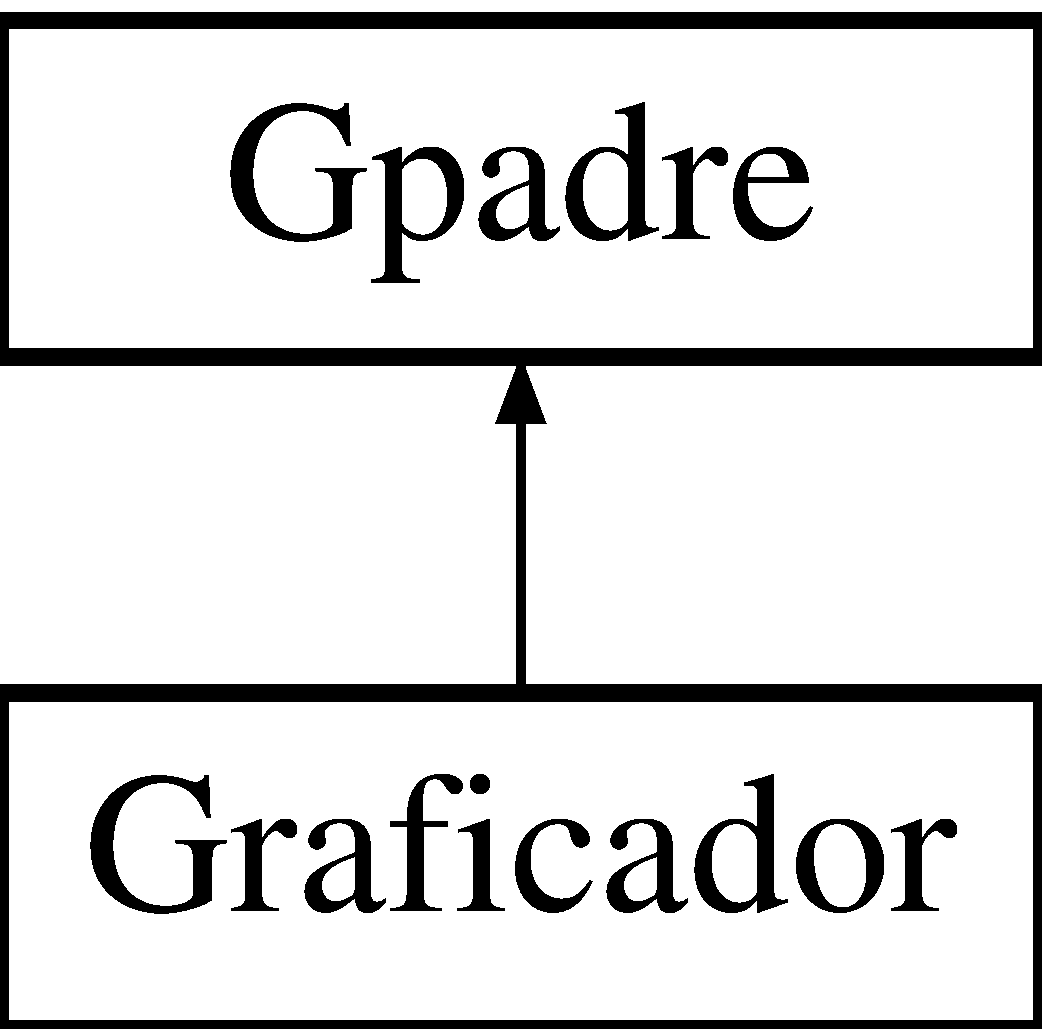
\includegraphics[height=2.000000cm]{class_gpadre}
\end{center}
\end{figure}
\subsection*{Métodos públicos}
\begin{DoxyCompactItemize}
\item 
\hyperlink{class_gpadre_a0f32f7f4711cac9c26f68e3facd4cfa6}{Gpadre} ()
\end{DoxyCompactItemize}
\subsection*{Atributos públicos}
\begin{DoxyCompactItemize}
\item 
vtk\+Smart\+Pointer$<$ vtk\+Renderer $>$ \hyperlink{class_gpadre_acb2bafea1132fdda5e023edc5067c673}{renderer} = vtk\+Smart\+Pointer$<$vtk\+Renderer$>$\+::New()
\end{DoxyCompactItemize}
\subsection*{Métodos protegidos}
\begin{DoxyCompactItemize}
\item 
void \hyperlink{class_gpadre_a7f14881edc7efd75801b1734dd919126}{next\+\_\+point} (std\+::vector$<$ double $>$, vtk\+Smart\+Pointer$<$ vtk\+Points $>$)
\item 
vtk\+Structured\+Grid $\ast$ \hyperlink{class_gpadre_a9dd73d0f23f1217b6ce4b48bb3fb1a16}{set\+\_\+points} (vtk\+Points $\ast$, int, int, int)
\item 
void \hyperlink{class_gpadre_a083d739f47fa034916366e714ddf6737}{print\+\_\+grid} (vtk\+Structured\+Grid $\ast$)
\item 
vtk\+Smart\+Pointer$<$ vtk\+Actor $>$ \hyperlink{class_gpadre_ae4adbdbc81a5121ba96d93c884c0196e}{filtro\+\_\+puntos} (vtk\+Structured\+Grid $\ast$)
\item 
vtk\+Smart\+Pointer$<$ vtk\+Actor $>$ \hyperlink{class_gpadre_ad22a3d28e46be883935b638c35c0a9dd}{filtro\+\_\+lineas} (vtk\+Structured\+Grid $\ast$)
\item 
vtk\+Smart\+Pointer$<$ vtk\+Actor $>$ \hyperlink{class_gpadre_af108d3defe91516b543dd08cfc1f4c5c}{mapear} (vtk\+Smart\+Pointer$<$ vtk\+Structured\+Grid $>$)
\item 
vtk\+Smart\+Pointer$<$ vtk\+Axes\+Actor $>$ \hyperlink{class_gpadre_a165bbe5dcd20c4d77b0c4277f41f3b0e}{axes} ()
\item 
void \hyperlink{class_gpadre_a33060a2381e76b38f3883619cbb7b73f}{render} (std\+::vector$<$ vtk\+Smart\+Pointer$<$ vtk\+Actor $>$ $>$, bool)
\end{DoxyCompactItemize}
\subsection*{Atributos protegidos}
\begin{DoxyCompactItemize}
\item 
vtk\+Smart\+Pointer$<$ vtk\+Render\+Window $>$ \hyperlink{class_gpadre_af512cc11dc03408872e033cec640d8ba}{render\+Window} = vtk\+Smart\+Pointer$<$vtk\+Render\+Window$>$\+::New()
\item 
vtk\+Smart\+Pointer$<$ vtk\+Render\+Window\+Interactor $>$ \hyperlink{class_gpadre_a31b647d46719088a5cb59688cdb2fe8a}{render\+Window\+Interactor} = vtk\+Smart\+Pointer$<$vtk\+Render\+Window\+Interactor$>$\+::New()
\end{DoxyCompactItemize}


\subsection{Documentación del constructor y destructor}
\index{Gpadre@{Gpadre}!Gpadre@{Gpadre}}
\index{Gpadre@{Gpadre}!Gpadre@{Gpadre}}
\subsubsection[{\texorpdfstring{Gpadre()}{Gpadre()}}]{\setlength{\rightskip}{0pt plus 5cm}Gpadre\+::\+Gpadre (
\begin{DoxyParamCaption}
{}
\end{DoxyParamCaption}
)}\hypertarget{class_gpadre_a0f32f7f4711cac9c26f68e3facd4cfa6}{}\label{class_gpadre_a0f32f7f4711cac9c26f68e3facd4cfa6}


\subsection{Documentación de las funciones miembro}
\index{Gpadre@{Gpadre}!axes@{axes}}
\index{axes@{axes}!Gpadre@{Gpadre}}
\subsubsection[{\texorpdfstring{axes()}{axes()}}]{\setlength{\rightskip}{0pt plus 5cm}vtk\+Smart\+Pointer$<$ vtk\+Axes\+Actor $>$ Gpadre\+::axes (
\begin{DoxyParamCaption}
{}
\end{DoxyParamCaption}
)\hspace{0.3cm}{\ttfamily [protected]}}\hypertarget{class_gpadre_a165bbe5dcd20c4d77b0c4277f41f3b0e}{}\label{class_gpadre_a165bbe5dcd20c4d77b0c4277f41f3b0e}
\index{Gpadre@{Gpadre}!filtro\+\_\+lineas@{filtro\+\_\+lineas}}
\index{filtro\+\_\+lineas@{filtro\+\_\+lineas}!Gpadre@{Gpadre}}
\subsubsection[{\texorpdfstring{filtro\+\_\+lineas(vtk\+Structured\+Grid $\ast$)}{filtro_lineas(vtkStructuredGrid *)}}]{\setlength{\rightskip}{0pt plus 5cm}vtk\+Smart\+Pointer$<$ vtk\+Actor $>$ Gpadre\+::filtro\+\_\+lineas (
\begin{DoxyParamCaption}
\item[{vtk\+Structured\+Grid $\ast$}]{structured\+Grid}
\end{DoxyParamCaption}
)\hspace{0.3cm}{\ttfamily [protected]}}\hypertarget{class_gpadre_ad22a3d28e46be883935b638c35c0a9dd}{}\label{class_gpadre_ad22a3d28e46be883935b638c35c0a9dd}
\index{Gpadre@{Gpadre}!filtro\+\_\+puntos@{filtro\+\_\+puntos}}
\index{filtro\+\_\+puntos@{filtro\+\_\+puntos}!Gpadre@{Gpadre}}
\subsubsection[{\texorpdfstring{filtro\+\_\+puntos(vtk\+Structured\+Grid $\ast$)}{filtro_puntos(vtkStructuredGrid *)}}]{\setlength{\rightskip}{0pt plus 5cm}vtk\+Smart\+Pointer$<$ vtk\+Actor $>$ Gpadre\+::filtro\+\_\+puntos (
\begin{DoxyParamCaption}
\item[{vtk\+Structured\+Grid $\ast$}]{structured\+Grid}
\end{DoxyParamCaption}
)\hspace{0.3cm}{\ttfamily [protected]}}\hypertarget{class_gpadre_ae4adbdbc81a5121ba96d93c884c0196e}{}\label{class_gpadre_ae4adbdbc81a5121ba96d93c884c0196e}
\index{Gpadre@{Gpadre}!mapear@{mapear}}
\index{mapear@{mapear}!Gpadre@{Gpadre}}
\subsubsection[{\texorpdfstring{mapear(vtk\+Smart\+Pointer$<$ vtk\+Structured\+Grid $>$)}{mapear(vtkSmartPointer< vtkStructuredGrid >)}}]{\setlength{\rightskip}{0pt plus 5cm}vtk\+Smart\+Pointer$<$ vtk\+Actor $>$ Gpadre\+::mapear (
\begin{DoxyParamCaption}
\item[{vtk\+Smart\+Pointer$<$ vtk\+Structured\+Grid $>$}]{grid}
\end{DoxyParamCaption}
)\hspace{0.3cm}{\ttfamily [protected]}}\hypertarget{class_gpadre_af108d3defe91516b543dd08cfc1f4c5c}{}\label{class_gpadre_af108d3defe91516b543dd08cfc1f4c5c}
\index{Gpadre@{Gpadre}!next\+\_\+point@{next\+\_\+point}}
\index{next\+\_\+point@{next\+\_\+point}!Gpadre@{Gpadre}}
\subsubsection[{\texorpdfstring{next\+\_\+point(std\+::vector$<$ double $>$, vtk\+Smart\+Pointer$<$ vtk\+Points $>$)}{next_point(std::vector< double >, vtkSmartPointer< vtkPoints >)}}]{\setlength{\rightskip}{0pt plus 5cm}void Gpadre\+::next\+\_\+point (
\begin{DoxyParamCaption}
\item[{std\+::vector$<$ double $>$}]{vec, }
\item[{vtk\+Smart\+Pointer$<$ vtk\+Points $>$}]{pointss}
\end{DoxyParamCaption}
)\hspace{0.3cm}{\ttfamily [protected]}}\hypertarget{class_gpadre_a7f14881edc7efd75801b1734dd919126}{}\label{class_gpadre_a7f14881edc7efd75801b1734dd919126}
\index{Gpadre@{Gpadre}!print\+\_\+grid@{print\+\_\+grid}}
\index{print\+\_\+grid@{print\+\_\+grid}!Gpadre@{Gpadre}}
\subsubsection[{\texorpdfstring{print\+\_\+grid(vtk\+Structured\+Grid $\ast$)}{print_grid(vtkStructuredGrid *)}}]{\setlength{\rightskip}{0pt plus 5cm}void Gpadre\+::print\+\_\+grid (
\begin{DoxyParamCaption}
\item[{vtk\+Structured\+Grid $\ast$}]{structured\+Grid}
\end{DoxyParamCaption}
)\hspace{0.3cm}{\ttfamily [protected]}}\hypertarget{class_gpadre_a083d739f47fa034916366e714ddf6737}{}\label{class_gpadre_a083d739f47fa034916366e714ddf6737}
\index{Gpadre@{Gpadre}!render@{render}}
\index{render@{render}!Gpadre@{Gpadre}}
\subsubsection[{\texorpdfstring{render(std\+::vector$<$ vtk\+Smart\+Pointer$<$ vtk\+Actor $>$ $>$, bool)}{render(std::vector< vtkSmartPointer< vtkActor > >, bool)}}]{\setlength{\rightskip}{0pt plus 5cm}void Gpadre\+::render (
\begin{DoxyParamCaption}
\item[{std\+::vector$<$ vtk\+Smart\+Pointer$<$ vtk\+Actor $>$ $>$}]{actors, }
\item[{bool}]{mostrar}
\end{DoxyParamCaption}
)\hspace{0.3cm}{\ttfamily [protected]}}\hypertarget{class_gpadre_a33060a2381e76b38f3883619cbb7b73f}{}\label{class_gpadre_a33060a2381e76b38f3883619cbb7b73f}
\index{Gpadre@{Gpadre}!set\+\_\+points@{set\+\_\+points}}
\index{set\+\_\+points@{set\+\_\+points}!Gpadre@{Gpadre}}
\subsubsection[{\texorpdfstring{set\+\_\+points(vtk\+Points $\ast$, int, int, int)}{set_points(vtkPoints *, int, int, int)}}]{\setlength{\rightskip}{0pt plus 5cm}vtk\+Structured\+Grid $\ast$ Gpadre\+::set\+\_\+points (
\begin{DoxyParamCaption}
\item[{vtk\+Points $\ast$}]{points, }
\item[{int}]{numi, }
\item[{int}]{numj, }
\item[{int}]{numk}
\end{DoxyParamCaption}
)\hspace{0.3cm}{\ttfamily [protected]}}\hypertarget{class_gpadre_a9dd73d0f23f1217b6ce4b48bb3fb1a16}{}\label{class_gpadre_a9dd73d0f23f1217b6ce4b48bb3fb1a16}


\subsection{Documentación de los datos miembro}
\index{Gpadre@{Gpadre}!renderer@{renderer}}
\index{renderer@{renderer}!Gpadre@{Gpadre}}
\subsubsection[{\texorpdfstring{renderer}{renderer}}]{\setlength{\rightskip}{0pt plus 5cm}vtk\+Smart\+Pointer$<$vtk\+Renderer$>$ Gpadre\+::renderer = vtk\+Smart\+Pointer$<$vtk\+Renderer$>$\+::New()}\hypertarget{class_gpadre_acb2bafea1132fdda5e023edc5067c673}{}\label{class_gpadre_acb2bafea1132fdda5e023edc5067c673}
\index{Gpadre@{Gpadre}!render\+Window@{render\+Window}}
\index{render\+Window@{render\+Window}!Gpadre@{Gpadre}}
\subsubsection[{\texorpdfstring{render\+Window}{renderWindow}}]{\setlength{\rightskip}{0pt plus 5cm}vtk\+Smart\+Pointer$<$vtk\+Render\+Window$>$ Gpadre\+::render\+Window = vtk\+Smart\+Pointer$<$vtk\+Render\+Window$>$\+::New()\hspace{0.3cm}{\ttfamily [protected]}}\hypertarget{class_gpadre_af512cc11dc03408872e033cec640d8ba}{}\label{class_gpadre_af512cc11dc03408872e033cec640d8ba}
\index{Gpadre@{Gpadre}!render\+Window\+Interactor@{render\+Window\+Interactor}}
\index{render\+Window\+Interactor@{render\+Window\+Interactor}!Gpadre@{Gpadre}}
\subsubsection[{\texorpdfstring{render\+Window\+Interactor}{renderWindowInteractor}}]{\setlength{\rightskip}{0pt plus 5cm}vtk\+Smart\+Pointer$<$vtk\+Render\+Window\+Interactor$>$ Gpadre\+::render\+Window\+Interactor = vtk\+Smart\+Pointer$<$vtk\+Render\+Window\+Interactor$>$\+::New()\hspace{0.3cm}{\ttfamily [protected]}}\hypertarget{class_gpadre_a31b647d46719088a5cb59688cdb2fe8a}{}\label{class_gpadre_a31b647d46719088a5cb59688cdb2fe8a}


La documentación para esta clase fue generada a partir de los siguientes ficheros\+:\begin{DoxyCompactItemize}
\item 
include/\hyperlink{gpadre_8h}{gpadre.\+h}\item 
src/\hyperlink{gpadre_8cpp}{gpadre.\+cpp}\end{DoxyCompactItemize}

\hypertarget{class_graficador}{}\section{Referencia de la Clase Graficador}
\label{class_graficador}\index{Graficador@{Graficador}}


{\ttfamily \#include $<$graficador.\+h$>$}

Diagrama de herencias de Graficador\begin{figure}[H]
\begin{center}
\leavevmode
\includegraphics[height=2.000000cm]{class_graficador}
\end{center}
\end{figure}
\subsection*{Métodos públicos}
\begin{DoxyCompactItemize}
\item 
\hyperlink{class_graficador_a62158abce60f946c3fd7893f2689e138}{Graficador} ()
\item 
void \hyperlink{class_graficador_a099289e888f91f94e377fd26d4cefaca}{crear} (std\+::vector$<$ std\+::vector$<$ double $>$$>$, int, int)
\item 
void \hyperlink{class_graficador_a799d3f27e186e07c2841aa8edbbf641f}{add\+\_\+filtros} ()
\item 
void \hyperlink{class_graficador_a47a1e61b68a8e1d346c2b0d21ff11d01}{add\+\_\+axes} ()
\item 
void \hyperlink{class_graficador_a74fa4bf9dff4b44b521a04a1cc0200a5}{renderizar} (bool mostrar=true)
\item 
void \hyperlink{class_graficador_a70f37ffd12170c31155c44f2aea11b93}{clean} ()
\end{DoxyCompactItemize}
\subsection*{Atributos públicos}
\begin{DoxyCompactItemize}
\item 
std\+::vector$<$ vtk\+Smart\+Pointer$<$ vtk\+Actor $>$ $>$ \hyperlink{class_graficador_af324352821c6e39961ed6977e50e9582}{actores}
\item 
vtk\+Smart\+Pointer$<$ vtk\+Structured\+Grid $>$ \hyperlink{class_graficador_aeb8321dafc848939f900bea4721142da}{structured\+Grid} = vtk\+Smart\+Pointer$<$vtk\+Structured\+Grid$>$\+::New()
\item 
vtk\+Smart\+Pointer$<$ vtk\+Camera $>$ \hyperlink{class_graficador_aeb158420087549f052e29a6739ea2f75}{camera} = vtk\+Smart\+Pointer$<$vtk\+Camera$>$\+::New()
\item 
vtk\+Smart\+Pointer$<$ vtk\+Unsigned\+Char\+Array $>$ \hyperlink{class_graficador_a48b78d03ae2e04e5032ed685f8fd8643}{colors} = vtk\+Smart\+Pointer$<$vtk\+Unsigned\+Char\+Array$>$\+::New()
\end{DoxyCompactItemize}
\subsection*{Otros miembros heredados}


\subsection{Documentación del constructor y destructor}
\index{Graficador@{Graficador}!Graficador@{Graficador}}
\index{Graficador@{Graficador}!Graficador@{Graficador}}
\subsubsection[{\texorpdfstring{Graficador()}{Graficador()}}]{\setlength{\rightskip}{0pt plus 5cm}Graficador\+::\+Graficador (
\begin{DoxyParamCaption}
{}
\end{DoxyParamCaption}
)}\hypertarget{class_graficador_a62158abce60f946c3fd7893f2689e138}{}\label{class_graficador_a62158abce60f946c3fd7893f2689e138}


\subsection{Documentación de las funciones miembro}
\index{Graficador@{Graficador}!add\+\_\+axes@{add\+\_\+axes}}
\index{add\+\_\+axes@{add\+\_\+axes}!Graficador@{Graficador}}
\subsubsection[{\texorpdfstring{add\+\_\+axes()}{add_axes()}}]{\setlength{\rightskip}{0pt plus 5cm}void Graficador\+::add\+\_\+axes (
\begin{DoxyParamCaption}
{}
\end{DoxyParamCaption}
)}\hypertarget{class_graficador_a47a1e61b68a8e1d346c2b0d21ff11d01}{}\label{class_graficador_a47a1e61b68a8e1d346c2b0d21ff11d01}
\index{Graficador@{Graficador}!add\+\_\+filtros@{add\+\_\+filtros}}
\index{add\+\_\+filtros@{add\+\_\+filtros}!Graficador@{Graficador}}
\subsubsection[{\texorpdfstring{add\+\_\+filtros()}{add_filtros()}}]{\setlength{\rightskip}{0pt plus 5cm}void Graficador\+::add\+\_\+filtros (
\begin{DoxyParamCaption}
{}
\end{DoxyParamCaption}
)}\hypertarget{class_graficador_a799d3f27e186e07c2841aa8edbbf641f}{}\label{class_graficador_a799d3f27e186e07c2841aa8edbbf641f}
\index{Graficador@{Graficador}!clean@{clean}}
\index{clean@{clean}!Graficador@{Graficador}}
\subsubsection[{\texorpdfstring{clean()}{clean()}}]{\setlength{\rightskip}{0pt plus 5cm}void Graficador\+::clean (
\begin{DoxyParamCaption}
{}
\end{DoxyParamCaption}
)}\hypertarget{class_graficador_a70f37ffd12170c31155c44f2aea11b93}{}\label{class_graficador_a70f37ffd12170c31155c44f2aea11b93}
\index{Graficador@{Graficador}!crear@{crear}}
\index{crear@{crear}!Graficador@{Graficador}}
\subsubsection[{\texorpdfstring{crear(std\+::vector$<$ std\+::vector$<$ double $>$$>$, int, int)}{crear(std::vector< std::vector< double >>, int, int)}}]{\setlength{\rightskip}{0pt plus 5cm}void Graficador\+::crear (
\begin{DoxyParamCaption}
\item[{std\+::vector$<$ std\+::vector$<$ double $>$$>$}]{vec, }
\item[{int}]{x, }
\item[{int}]{y}
\end{DoxyParamCaption}
)}\hypertarget{class_graficador_a099289e888f91f94e377fd26d4cefaca}{}\label{class_graficador_a099289e888f91f94e377fd26d4cefaca}
\index{Graficador@{Graficador}!renderizar@{renderizar}}
\index{renderizar@{renderizar}!Graficador@{Graficador}}
\subsubsection[{\texorpdfstring{renderizar(bool mostrar=true)}{renderizar(bool mostrar=true)}}]{\setlength{\rightskip}{0pt plus 5cm}void Graficador\+::renderizar (
\begin{DoxyParamCaption}
\item[{bool}]{mostrar = {\ttfamily true}}
\end{DoxyParamCaption}
)}\hypertarget{class_graficador_a74fa4bf9dff4b44b521a04a1cc0200a5}{}\label{class_graficador_a74fa4bf9dff4b44b521a04a1cc0200a5}


\subsection{Documentación de los datos miembro}
\index{Graficador@{Graficador}!actores@{actores}}
\index{actores@{actores}!Graficador@{Graficador}}
\subsubsection[{\texorpdfstring{actores}{actores}}]{\setlength{\rightskip}{0pt plus 5cm}std\+::vector$<$vtk\+Smart\+Pointer$<$vtk\+Actor$>$ $>$ Graficador\+::actores}\hypertarget{class_graficador_af324352821c6e39961ed6977e50e9582}{}\label{class_graficador_af324352821c6e39961ed6977e50e9582}
\index{Graficador@{Graficador}!camera@{camera}}
\index{camera@{camera}!Graficador@{Graficador}}
\subsubsection[{\texorpdfstring{camera}{camera}}]{\setlength{\rightskip}{0pt plus 5cm}vtk\+Smart\+Pointer$<$vtk\+Camera$>$ Graficador\+::camera = vtk\+Smart\+Pointer$<$vtk\+Camera$>$\+::New()}\hypertarget{class_graficador_aeb158420087549f052e29a6739ea2f75}{}\label{class_graficador_aeb158420087549f052e29a6739ea2f75}
\index{Graficador@{Graficador}!colors@{colors}}
\index{colors@{colors}!Graficador@{Graficador}}
\subsubsection[{\texorpdfstring{colors}{colors}}]{\setlength{\rightskip}{0pt plus 5cm}vtk\+Smart\+Pointer$<$vtk\+Unsigned\+Char\+Array$>$ Graficador\+::colors = vtk\+Smart\+Pointer$<$vtk\+Unsigned\+Char\+Array$>$\+::New()}\hypertarget{class_graficador_a48b78d03ae2e04e5032ed685f8fd8643}{}\label{class_graficador_a48b78d03ae2e04e5032ed685f8fd8643}
\index{Graficador@{Graficador}!structured\+Grid@{structured\+Grid}}
\index{structured\+Grid@{structured\+Grid}!Graficador@{Graficador}}
\subsubsection[{\texorpdfstring{structured\+Grid}{structuredGrid}}]{\setlength{\rightskip}{0pt plus 5cm}vtk\+Smart\+Pointer$<$vtk\+Structured\+Grid$>$ Graficador\+::structured\+Grid = vtk\+Smart\+Pointer$<$vtk\+Structured\+Grid$>$\+::New()}\hypertarget{class_graficador_aeb8321dafc848939f900bea4721142da}{}\label{class_graficador_aeb8321dafc848939f900bea4721142da}


La documentación para esta clase fue generada a partir de los siguientes ficheros\+:\begin{DoxyCompactItemize}
\item 
include/\hyperlink{graficador_8h}{graficador.\+h}\item 
src/\hyperlink{graficador_8cpp}{graficador.\+cpp}\end{DoxyCompactItemize}

\hypertarget{class_graficador1}{}\section{Referencia de la Clase Graficador1}
\label{class_graficador1}\index{Graficador1@{Graficador1}}


{\ttfamily \#include $<$graficador1.\+h$>$}

\subsection*{Métodos públicos}
\begin{DoxyCompactItemize}
\item 
\hyperlink{class_graficador1_aad669b9e0784dd67bf7aadf65a657608}{Graficador1} ()
\item 
void \hyperlink{class_graficador1_a5b79063a4630ab7d01cb6e4f9e7b7a1f}{puntos2d} ()
\item 
void \hyperlink{class_graficador1_aa2af594975f59373167af2de434ad665}{crearpolilinea} ()
\item 
void \hyperlink{class_graficador1_afa15e469dd3579558eae1b303180e7bd}{insertar\+\_\+punto} (double, double, double)
\item 
void \hyperlink{class_graficador1_a400a046298f47f30a350d9da3f60c541}{insertar\+\_\+polilinea} (int)
\item 
void \hyperlink{class_graficador1_ae8416d64e9889d4eef20a53bf0251831}{set\+\_\+polilinea} (int)
\item 
void \hyperlink{class_graficador1_a66e079687b749600be62080387a4049c}{clean} ()
\item 
double \hyperlink{class_graficador1_a61617b0f3755ffbb05c07d94515b6185}{cuadrado} (double)
\end{DoxyCompactItemize}
\subsection*{Atributos públicos}
\begin{DoxyCompactItemize}
\item 
vtk\+Smart\+Pointer$<$ vtk\+Actor $>$ \hyperlink{class_graficador1_a8ae74354def8d4b9cf9a5888a3d5f7f6}{actor} = vtk\+Smart\+Pointer$<$vtk\+Actor$>$\+::New()
\item 
vtk\+Smart\+Pointer$<$ vtk\+Renderer $>$ \hyperlink{class_graficador1_a37f34d5e7cc90e5ce119de4b3c5e99a5}{renderer} = vtk\+Smart\+Pointer$<$vtk\+Renderer$>$\+::New()
\item 
vtk\+Smart\+Pointer$<$ vtk\+Axes\+Actor $>$ \hyperlink{class_graficador1_a2e21aceca117ab118ac832fab7069222}{axes} = vtk\+Smart\+Pointer$<$vtk\+Axes\+Actor$>$\+::New()
\item 
vtk\+Smart\+Pointer$<$ vtk\+Cell\+Array $>$ \hyperlink{class_graficador1_a0cfb1ed1aa24256300eba63ec3961be8}{cells} = vtk\+Smart\+Pointer$<$vtk\+Cell\+Array$>$\+::New()
\item 
vtk\+Smart\+Pointer$<$ vtk\+Camera $>$ \hyperlink{class_graficador1_a84c019e93c84cebb467b96fe51f7e00f}{camera} = vtk\+Smart\+Pointer$<$vtk\+Camera$>$\+::New()
\item 
vtk\+Smart\+Pointer$<$ vtk\+Poly\+Data $>$ \hyperlink{class_graficador1_a4a2f54d79982b0df5f89bc8ccc94f2ac}{poly\+Data} = vtk\+Smart\+Pointer$<$vtk\+Poly\+Data$>$\+::New()
\item 
vtk\+Smart\+Pointer$<$ vtk\+Poly\+Line $>$ \hyperlink{class_graficador1_a8104c16db84a43865caad8ee2a3956b9}{poly\+Line} = vtk\+Smart\+Pointer$<$vtk\+Poly\+Line$>$\+::New()
\item 
vtk\+Smart\+Pointer$<$ vtk\+Poly\+Data\+Mapper $>$ \hyperlink{class_graficador1_a1cf22b3f22afd3b46c4e7c2e2d24c5e7}{mapper} = vtk\+Smart\+Pointer$<$vtk\+Poly\+Data\+Mapper$>$\+::New()
\item 
vtk\+Smart\+Pointer$<$ vtk\+Unsigned\+Char\+Array $>$ \hyperlink{class_graficador1_a13a6fb8216c7abf42e3e0ce8a39df1b8}{colors} = vtk\+Smart\+Pointer$<$vtk\+Unsigned\+Char\+Array$>$\+::New()
\item 
vtk\+Smart\+Pointer$<$ vtk\+Points $>$ \hyperlink{class_graficador1_a27673da414293c9c86dffc22f8d18b60}{points} = vtk\+Smart\+Pointer$<$vtk\+Points$>$\+::New()
\end{DoxyCompactItemize}


\subsection{Documentación del constructor y destructor}
\index{Graficador1@{Graficador1}!Graficador1@{Graficador1}}
\index{Graficador1@{Graficador1}!Graficador1@{Graficador1}}
\subsubsection[{\texorpdfstring{Graficador1()}{Graficador1()}}]{\setlength{\rightskip}{0pt plus 5cm}Graficador1\+::\+Graficador1 (
\begin{DoxyParamCaption}
{}
\end{DoxyParamCaption}
)}\hypertarget{class_graficador1_aad669b9e0784dd67bf7aadf65a657608}{}\label{class_graficador1_aad669b9e0784dd67bf7aadf65a657608}


\subsection{Documentación de las funciones miembro}
\index{Graficador1@{Graficador1}!clean@{clean}}
\index{clean@{clean}!Graficador1@{Graficador1}}
\subsubsection[{\texorpdfstring{clean()}{clean()}}]{\setlength{\rightskip}{0pt plus 5cm}void Graficador1\+::clean (
\begin{DoxyParamCaption}
{}
\end{DoxyParamCaption}
)}\hypertarget{class_graficador1_a66e079687b749600be62080387a4049c}{}\label{class_graficador1_a66e079687b749600be62080387a4049c}
\index{Graficador1@{Graficador1}!crearpolilinea@{crearpolilinea}}
\index{crearpolilinea@{crearpolilinea}!Graficador1@{Graficador1}}
\subsubsection[{\texorpdfstring{crearpolilinea()}{crearpolilinea()}}]{\setlength{\rightskip}{0pt plus 5cm}void Graficador1\+::crearpolilinea (
\begin{DoxyParamCaption}
{}
\end{DoxyParamCaption}
)}\hypertarget{class_graficador1_aa2af594975f59373167af2de434ad665}{}\label{class_graficador1_aa2af594975f59373167af2de434ad665}
\index{Graficador1@{Graficador1}!cuadrado@{cuadrado}}
\index{cuadrado@{cuadrado}!Graficador1@{Graficador1}}
\subsubsection[{\texorpdfstring{cuadrado(double)}{cuadrado(double)}}]{\setlength{\rightskip}{0pt plus 5cm}double Graficador1\+::cuadrado (
\begin{DoxyParamCaption}
\item[{double}]{}
\end{DoxyParamCaption}
)}\hypertarget{class_graficador1_a61617b0f3755ffbb05c07d94515b6185}{}\label{class_graficador1_a61617b0f3755ffbb05c07d94515b6185}
\index{Graficador1@{Graficador1}!insertar\+\_\+polilinea@{insertar\+\_\+polilinea}}
\index{insertar\+\_\+polilinea@{insertar\+\_\+polilinea}!Graficador1@{Graficador1}}
\subsubsection[{\texorpdfstring{insertar\+\_\+polilinea(int)}{insertar_polilinea(int)}}]{\setlength{\rightskip}{0pt plus 5cm}void Graficador1\+::insertar\+\_\+polilinea (
\begin{DoxyParamCaption}
\item[{int}]{}
\end{DoxyParamCaption}
)}\hypertarget{class_graficador1_a400a046298f47f30a350d9da3f60c541}{}\label{class_graficador1_a400a046298f47f30a350d9da3f60c541}
\index{Graficador1@{Graficador1}!insertar\+\_\+punto@{insertar\+\_\+punto}}
\index{insertar\+\_\+punto@{insertar\+\_\+punto}!Graficador1@{Graficador1}}
\subsubsection[{\texorpdfstring{insertar\+\_\+punto(double, double, double)}{insertar_punto(double, double, double)}}]{\setlength{\rightskip}{0pt plus 5cm}void Graficador1\+::insertar\+\_\+punto (
\begin{DoxyParamCaption}
\item[{double}]{, }
\item[{double}]{, }
\item[{double}]{}
\end{DoxyParamCaption}
)}\hypertarget{class_graficador1_afa15e469dd3579558eae1b303180e7bd}{}\label{class_graficador1_afa15e469dd3579558eae1b303180e7bd}
\index{Graficador1@{Graficador1}!puntos2d@{puntos2d}}
\index{puntos2d@{puntos2d}!Graficador1@{Graficador1}}
\subsubsection[{\texorpdfstring{puntos2d()}{puntos2d()}}]{\setlength{\rightskip}{0pt plus 5cm}void Graficador1\+::puntos2d (
\begin{DoxyParamCaption}
{}
\end{DoxyParamCaption}
)}\hypertarget{class_graficador1_a5b79063a4630ab7d01cb6e4f9e7b7a1f}{}\label{class_graficador1_a5b79063a4630ab7d01cb6e4f9e7b7a1f}
\index{Graficador1@{Graficador1}!set\+\_\+polilinea@{set\+\_\+polilinea}}
\index{set\+\_\+polilinea@{set\+\_\+polilinea}!Graficador1@{Graficador1}}
\subsubsection[{\texorpdfstring{set\+\_\+polilinea(int)}{set_polilinea(int)}}]{\setlength{\rightskip}{0pt plus 5cm}void Graficador1\+::set\+\_\+polilinea (
\begin{DoxyParamCaption}
\item[{int}]{}
\end{DoxyParamCaption}
)}\hypertarget{class_graficador1_ae8416d64e9889d4eef20a53bf0251831}{}\label{class_graficador1_ae8416d64e9889d4eef20a53bf0251831}


\subsection{Documentación de los datos miembro}
\index{Graficador1@{Graficador1}!actor@{actor}}
\index{actor@{actor}!Graficador1@{Graficador1}}
\subsubsection[{\texorpdfstring{actor}{actor}}]{\setlength{\rightskip}{0pt plus 5cm}vtk\+Smart\+Pointer$<$vtk\+Actor$>$ Graficador1\+::actor = vtk\+Smart\+Pointer$<$vtk\+Actor$>$\+::New()}\hypertarget{class_graficador1_a8ae74354def8d4b9cf9a5888a3d5f7f6}{}\label{class_graficador1_a8ae74354def8d4b9cf9a5888a3d5f7f6}
\index{Graficador1@{Graficador1}!axes@{axes}}
\index{axes@{axes}!Graficador1@{Graficador1}}
\subsubsection[{\texorpdfstring{axes}{axes}}]{\setlength{\rightskip}{0pt plus 5cm}vtk\+Smart\+Pointer$<$vtk\+Axes\+Actor$>$ Graficador1\+::axes = vtk\+Smart\+Pointer$<$vtk\+Axes\+Actor$>$\+::New()}\hypertarget{class_graficador1_a2e21aceca117ab118ac832fab7069222}{}\label{class_graficador1_a2e21aceca117ab118ac832fab7069222}
\index{Graficador1@{Graficador1}!camera@{camera}}
\index{camera@{camera}!Graficador1@{Graficador1}}
\subsubsection[{\texorpdfstring{camera}{camera}}]{\setlength{\rightskip}{0pt plus 5cm}vtk\+Smart\+Pointer$<$vtk\+Camera$>$ Graficador1\+::camera = vtk\+Smart\+Pointer$<$vtk\+Camera$>$\+::New()}\hypertarget{class_graficador1_a84c019e93c84cebb467b96fe51f7e00f}{}\label{class_graficador1_a84c019e93c84cebb467b96fe51f7e00f}
\index{Graficador1@{Graficador1}!cells@{cells}}
\index{cells@{cells}!Graficador1@{Graficador1}}
\subsubsection[{\texorpdfstring{cells}{cells}}]{\setlength{\rightskip}{0pt plus 5cm}vtk\+Smart\+Pointer$<$vtk\+Cell\+Array$>$ Graficador1\+::cells = vtk\+Smart\+Pointer$<$vtk\+Cell\+Array$>$\+::New()}\hypertarget{class_graficador1_a0cfb1ed1aa24256300eba63ec3961be8}{}\label{class_graficador1_a0cfb1ed1aa24256300eba63ec3961be8}
\index{Graficador1@{Graficador1}!colors@{colors}}
\index{colors@{colors}!Graficador1@{Graficador1}}
\subsubsection[{\texorpdfstring{colors}{colors}}]{\setlength{\rightskip}{0pt plus 5cm}vtk\+Smart\+Pointer$<$vtk\+Unsigned\+Char\+Array$>$ Graficador1\+::colors = vtk\+Smart\+Pointer$<$vtk\+Unsigned\+Char\+Array$>$\+::New()}\hypertarget{class_graficador1_a13a6fb8216c7abf42e3e0ce8a39df1b8}{}\label{class_graficador1_a13a6fb8216c7abf42e3e0ce8a39df1b8}
\index{Graficador1@{Graficador1}!mapper@{mapper}}
\index{mapper@{mapper}!Graficador1@{Graficador1}}
\subsubsection[{\texorpdfstring{mapper}{mapper}}]{\setlength{\rightskip}{0pt plus 5cm}vtk\+Smart\+Pointer$<$vtk\+Poly\+Data\+Mapper$>$ Graficador1\+::mapper = vtk\+Smart\+Pointer$<$vtk\+Poly\+Data\+Mapper$>$\+::New()}\hypertarget{class_graficador1_a1cf22b3f22afd3b46c4e7c2e2d24c5e7}{}\label{class_graficador1_a1cf22b3f22afd3b46c4e7c2e2d24c5e7}
\index{Graficador1@{Graficador1}!points@{points}}
\index{points@{points}!Graficador1@{Graficador1}}
\subsubsection[{\texorpdfstring{points}{points}}]{\setlength{\rightskip}{0pt plus 5cm}vtk\+Smart\+Pointer$<$vtk\+Points$>$ Graficador1\+::points = vtk\+Smart\+Pointer$<$vtk\+Points$>$\+::New()}\hypertarget{class_graficador1_a27673da414293c9c86dffc22f8d18b60}{}\label{class_graficador1_a27673da414293c9c86dffc22f8d18b60}
\index{Graficador1@{Graficador1}!poly\+Data@{poly\+Data}}
\index{poly\+Data@{poly\+Data}!Graficador1@{Graficador1}}
\subsubsection[{\texorpdfstring{poly\+Data}{polyData}}]{\setlength{\rightskip}{0pt plus 5cm}vtk\+Smart\+Pointer$<$vtk\+Poly\+Data$>$ Graficador1\+::poly\+Data = vtk\+Smart\+Pointer$<$vtk\+Poly\+Data$>$\+::New()}\hypertarget{class_graficador1_a4a2f54d79982b0df5f89bc8ccc94f2ac}{}\label{class_graficador1_a4a2f54d79982b0df5f89bc8ccc94f2ac}
\index{Graficador1@{Graficador1}!poly\+Line@{poly\+Line}}
\index{poly\+Line@{poly\+Line}!Graficador1@{Graficador1}}
\subsubsection[{\texorpdfstring{poly\+Line}{polyLine}}]{\setlength{\rightskip}{0pt plus 5cm}vtk\+Smart\+Pointer$<$vtk\+Poly\+Line$>$ Graficador1\+::poly\+Line = vtk\+Smart\+Pointer$<$vtk\+Poly\+Line$>$\+::New()}\hypertarget{class_graficador1_a8104c16db84a43865caad8ee2a3956b9}{}\label{class_graficador1_a8104c16db84a43865caad8ee2a3956b9}
\index{Graficador1@{Graficador1}!renderer@{renderer}}
\index{renderer@{renderer}!Graficador1@{Graficador1}}
\subsubsection[{\texorpdfstring{renderer}{renderer}}]{\setlength{\rightskip}{0pt plus 5cm}vtk\+Smart\+Pointer$<$vtk\+Renderer$>$ Graficador1\+::renderer = vtk\+Smart\+Pointer$<$vtk\+Renderer$>$\+::New()}\hypertarget{class_graficador1_a37f34d5e7cc90e5ce119de4b3c5e99a5}{}\label{class_graficador1_a37f34d5e7cc90e5ce119de4b3c5e99a5}


La documentación para esta clase fue generada a partir de los siguientes ficheros\+:\begin{DoxyCompactItemize}
\item 
include/\hyperlink{graficador1_8h}{graficador1.\+h}\item 
src/\hyperlink{graficador1_8cpp}{graficador1.\+cpp}\end{DoxyCompactItemize}

\hypertarget{class_interpretador}{}\section{Referencia de la Clase Interpretador}
\label{class_interpretador}\index{Interpretador@{Interpretador}}


{\ttfamily \#include $<$Interpretador.\+h$>$}

\subsection*{Métodos públicos}
\begin{DoxyCompactItemize}
\item 
\hyperlink{class_interpretador_a12d844a7ab8d634e96b57971c9aedd9e}{Interpretador} ()
\item 
virtual \hyperlink{class_interpretador_a7a3a27d4a51d961df2ad0dc5c9c67efd}{$\sim$\+Interpretador} ()
\item 
void \hyperlink{class_interpretador_a5fe0e48acd59f9e30f9a6d0b6fdc8fa2}{elim\+\_\+vacio} (std\+::vector$<$ string $>$ \&)
\item 
void \hyperlink{class_interpretador_a14fe65c1d966925c56248551d8e41d5d}{separar\+\_\+en\+\_\+dos} (std\+::vector$<$ string $>$ \&, string)
\item 
void \hyperlink{class_interpretador_ac3dba52e23ccd5f66e372562db17a0a6}{reverse\+\_\+string} (string \&)
\item 
bool \hyperlink{class_interpretador_a94fa9d2449766953dbb3806f9f8cff00}{buscar\+\_\+ope} (string, string, std\+::vector$<$ string $>$ \&)
\item 
void \hyperlink{class_interpretador_a5ad45a7156035ca33ed3cc30603c83e8}{transformar} (string text)
\item 
void \hyperlink{class_interpretador_ac096061ccb53d31d3e167994ff482992}{transformar} (string text, \hyperlink{class_nodo}{Nodo} $\ast$, bool)
\item 
double \hyperlink{class_interpretador_ac3b1cd0b89441d2f08ab721a5eb43143}{string\+\_\+to\+\_\+double} (string)
\item 
void \hyperlink{class_interpretador_a2d4e10b621a47802ba4e29eb0abd18c2}{elim\+\_\+parent} (string \&)
\item 
bool \hyperlink{class_interpretador_a70361935b6fd4bc539ed23e81b98dc4d}{esta\+\_\+en} (string text, string ope)
\item 
std\+::string \hyperlink{class_interpretador_ae91263671ef360654289dbf0e1e340ee}{verif\+\_\+sintaxis} (std\+::string)
\item 
void \hyperlink{class_interpretador_a50bdb39c90e92e8f92be71443339774c}{fix\+\_\+multi} (std\+::vector$<$ string $>$ \&)
\item 
std\+::vector$<$ string $>$ \hyperlink{class_interpretador_a131a8526e7eca0c2ebd36d5fd9f116df}{string\+\_\+to\+\_\+vector} (string)
\item 
void \hyperlink{class_interpretador_a56b129ed3210f94fafed102eeb68f633}{fix\+\_\+multiplicaciones} (std\+::vector$<$ string $>$ \&)
\item 
void \hyperlink{class_interpretador_aa89bcf45e7c07b712ca0d63e32ef098b}{fix\+\_\+negativos} (std\+::vector$<$ string $>$ \&)
\item 
void \hyperlink{class_interpretador_aa95dd4e2fe49213ff6d445f3fb69881d}{fix\+\_\+operaciones\+\_\+unarias} (std\+::vector$<$ string $>$ \&)
\item 
string \hyperlink{class_interpretador_a87e389afc6775a51deaea1c5730e9ecc}{get\+\_\+operador\+\_\+mayor\+\_\+prioridad} (std\+::vector$<$ string $>$)
\item 
int \hyperlink{class_interpretador_a2032902283b06008db2cad20050ecced}{get\+\_\+operador\+\_\+prioridad} (string)
\item 
bool \hyperlink{class_interpretador_a99c39d578dc93c193c7d5de164985e35}{es\+\_\+operador} (string)
\item 
bool \hyperlink{class_interpretador_a54276960e2c38150c3f337447414b2f0}{is\+\_\+number} (const std\+::string \&)
\item 
bool \hyperlink{class_interpretador_a7029c0ad73ed9ab55de3033073b169db}{is\+Alpha} (const string \&)
\item 
bool \hyperlink{class_interpretador_a2c47cecd7282c404a4fc858a303d9230}{es\+\_\+operador\+\_\+unario} (string)
\item 
bool \hyperlink{class_interpretador_aa376909fd2d36b41124af047055e5f34}{es\+\_\+operador\+\_\+binario} (string)
\item 
bool \hyperlink{class_interpretador_a256caa85f2333b3d5f98b50755fde5c8}{es\+\_\+expresion} (string)
\end{DoxyCompactItemize}
\subsection*{Atributos públicos}
\begin{DoxyCompactItemize}
\item 
map$<$ string, double($\ast$)(double)$>$ \hyperlink{class_interpretador_a69b4c0a967ebb3300bdd1a0d768be777}{funciones\+\_\+unarias}
\item 
map$<$ string, double($\ast$)(double, double)$>$ \hyperlink{class_interpretador_aae54d44f01e4c4b755ae133819b49d78}{funciones\+\_\+binarias}
\item 
map$<$ string, int $>$ \hyperlink{class_interpretador_a5ba0987e974f7eaba6376e0539466788}{prioridad\+\_\+funciones}
\item 
\hyperlink{classarbol__binario}{arbol\+\_\+binario} $\ast$ \hyperlink{class_interpretador_a95ae1c37ba98e88aeffec2807eb3f332}{tree}
\end{DoxyCompactItemize}


\subsection{Documentación del constructor y destructor}
\index{Interpretador@{Interpretador}!Interpretador@{Interpretador}}
\index{Interpretador@{Interpretador}!Interpretador@{Interpretador}}
\subsubsection[{\texorpdfstring{Interpretador()}{Interpretador()}}]{\setlength{\rightskip}{0pt plus 5cm}Interpretador\+::\+Interpretador (
\begin{DoxyParamCaption}
{}
\end{DoxyParamCaption}
)}\hypertarget{class_interpretador_a12d844a7ab8d634e96b57971c9aedd9e}{}\label{class_interpretador_a12d844a7ab8d634e96b57971c9aedd9e}
\index{Interpretador@{Interpretador}!````~Interpretador@{$\sim$\+Interpretador}}
\index{````~Interpretador@{$\sim$\+Interpretador}!Interpretador@{Interpretador}}
\subsubsection[{\texorpdfstring{$\sim$\+Interpretador()}{~Interpretador()}}]{\setlength{\rightskip}{0pt plus 5cm}Interpretador\+::$\sim$\+Interpretador (
\begin{DoxyParamCaption}
{}
\end{DoxyParamCaption}
)\hspace{0.3cm}{\ttfamily [virtual]}}\hypertarget{class_interpretador_a7a3a27d4a51d961df2ad0dc5c9c67efd}{}\label{class_interpretador_a7a3a27d4a51d961df2ad0dc5c9c67efd}


\subsection{Documentación de las funciones miembro}
\index{Interpretador@{Interpretador}!buscar\+\_\+ope@{buscar\+\_\+ope}}
\index{buscar\+\_\+ope@{buscar\+\_\+ope}!Interpretador@{Interpretador}}
\subsubsection[{\texorpdfstring{buscar\+\_\+ope(string, string, std\+::vector$<$ string $>$ \&)}{buscar_ope(string, string, std::vector< string > &)}}]{\setlength{\rightskip}{0pt plus 5cm}{\bf booleano} Interpretador\+::buscar\+\_\+ope (
\begin{DoxyParamCaption}
\item[{string}]{, }
\item[{string}]{, }
\item[{std\+::vector$<$ string $>$ \&}]{}
\end{DoxyParamCaption}
)}\hypertarget{class_interpretador_a94fa9d2449766953dbb3806f9f8cff00}{}\label{class_interpretador_a94fa9d2449766953dbb3806f9f8cff00}
\index{Interpretador@{Interpretador}!elim\+\_\+parent@{elim\+\_\+parent}}
\index{elim\+\_\+parent@{elim\+\_\+parent}!Interpretador@{Interpretador}}
\subsubsection[{\texorpdfstring{elim\+\_\+parent(string \&)}{elim_parent(string &)}}]{\setlength{\rightskip}{0pt plus 5cm}void Interpretador\+::elim\+\_\+parent (
\begin{DoxyParamCaption}
\item[{string \&}]{}
\end{DoxyParamCaption}
)}\hypertarget{class_interpretador_a2d4e10b621a47802ba4e29eb0abd18c2}{}\label{class_interpretador_a2d4e10b621a47802ba4e29eb0abd18c2}
\index{Interpretador@{Interpretador}!elim\+\_\+vacio@{elim\+\_\+vacio}}
\index{elim\+\_\+vacio@{elim\+\_\+vacio}!Interpretador@{Interpretador}}
\subsubsection[{\texorpdfstring{elim\+\_\+vacio(std\+::vector$<$ string $>$ \&)}{elim_vacio(std::vector< string > &)}}]{\setlength{\rightskip}{0pt plus 5cm}void Interpretador\+::elim\+\_\+vacio (
\begin{DoxyParamCaption}
\item[{std\+::vector$<$ string $>$ \&}]{v}
\end{DoxyParamCaption}
)}\hypertarget{class_interpretador_a5fe0e48acd59f9e30f9a6d0b6fdc8fa2}{}\label{class_interpretador_a5fe0e48acd59f9e30f9a6d0b6fdc8fa2}
\index{Interpretador@{Interpretador}!es\+\_\+expresion@{es\+\_\+expresion}}
\index{es\+\_\+expresion@{es\+\_\+expresion}!Interpretador@{Interpretador}}
\subsubsection[{\texorpdfstring{es\+\_\+expresion(string)}{es_expresion(string)}}]{\setlength{\rightskip}{0pt plus 5cm}bool Interpretador\+::es\+\_\+expresion (
\begin{DoxyParamCaption}
\item[{string}]{texto}
\end{DoxyParamCaption}
)}\hypertarget{class_interpretador_a256caa85f2333b3d5f98b50755fde5c8}{}\label{class_interpretador_a256caa85f2333b3d5f98b50755fde5c8}
\index{Interpretador@{Interpretador}!es\+\_\+operador@{es\+\_\+operador}}
\index{es\+\_\+operador@{es\+\_\+operador}!Interpretador@{Interpretador}}
\subsubsection[{\texorpdfstring{es\+\_\+operador(string)}{es_operador(string)}}]{\setlength{\rightskip}{0pt plus 5cm}bool Interpretador\+::es\+\_\+operador (
\begin{DoxyParamCaption}
\item[{string}]{oper}
\end{DoxyParamCaption}
)}\hypertarget{class_interpretador_a99c39d578dc93c193c7d5de164985e35}{}\label{class_interpretador_a99c39d578dc93c193c7d5de164985e35}
\index{Interpretador@{Interpretador}!es\+\_\+operador\+\_\+binario@{es\+\_\+operador\+\_\+binario}}
\index{es\+\_\+operador\+\_\+binario@{es\+\_\+operador\+\_\+binario}!Interpretador@{Interpretador}}
\subsubsection[{\texorpdfstring{es\+\_\+operador\+\_\+binario(string)}{es_operador_binario(string)}}]{\setlength{\rightskip}{0pt plus 5cm}bool Interpretador\+::es\+\_\+operador\+\_\+binario (
\begin{DoxyParamCaption}
\item[{string}]{oper}
\end{DoxyParamCaption}
)}\hypertarget{class_interpretador_aa376909fd2d36b41124af047055e5f34}{}\label{class_interpretador_aa376909fd2d36b41124af047055e5f34}
\index{Interpretador@{Interpretador}!es\+\_\+operador\+\_\+unario@{es\+\_\+operador\+\_\+unario}}
\index{es\+\_\+operador\+\_\+unario@{es\+\_\+operador\+\_\+unario}!Interpretador@{Interpretador}}
\subsubsection[{\texorpdfstring{es\+\_\+operador\+\_\+unario(string)}{es_operador_unario(string)}}]{\setlength{\rightskip}{0pt plus 5cm}bool Interpretador\+::es\+\_\+operador\+\_\+unario (
\begin{DoxyParamCaption}
\item[{string}]{oper}
\end{DoxyParamCaption}
)}\hypertarget{class_interpretador_a2c47cecd7282c404a4fc858a303d9230}{}\label{class_interpretador_a2c47cecd7282c404a4fc858a303d9230}
\index{Interpretador@{Interpretador}!esta\+\_\+en@{esta\+\_\+en}}
\index{esta\+\_\+en@{esta\+\_\+en}!Interpretador@{Interpretador}}
\subsubsection[{\texorpdfstring{esta\+\_\+en(string text, string ope)}{esta_en(string text, string ope)}}]{\setlength{\rightskip}{0pt plus 5cm}{\bf booleano} Interpretador\+::esta\+\_\+en (
\begin{DoxyParamCaption}
\item[{string}]{text, }
\item[{string}]{ope}
\end{DoxyParamCaption}
)}\hypertarget{class_interpretador_a70361935b6fd4bc539ed23e81b98dc4d}{}\label{class_interpretador_a70361935b6fd4bc539ed23e81b98dc4d}
\index{Interpretador@{Interpretador}!fix\+\_\+multi@{fix\+\_\+multi}}
\index{fix\+\_\+multi@{fix\+\_\+multi}!Interpretador@{Interpretador}}
\subsubsection[{\texorpdfstring{fix\+\_\+multi(std\+::vector$<$ string $>$ \&)}{fix_multi(std::vector< string > &)}}]{\setlength{\rightskip}{0pt plus 5cm}void Interpretador\+::fix\+\_\+multi (
\begin{DoxyParamCaption}
\item[{std\+::vector$<$ string $>$ \&}]{}
\end{DoxyParamCaption}
)}\hypertarget{class_interpretador_a50bdb39c90e92e8f92be71443339774c}{}\label{class_interpretador_a50bdb39c90e92e8f92be71443339774c}
\index{Interpretador@{Interpretador}!fix\+\_\+multiplicaciones@{fix\+\_\+multiplicaciones}}
\index{fix\+\_\+multiplicaciones@{fix\+\_\+multiplicaciones}!Interpretador@{Interpretador}}
\subsubsection[{\texorpdfstring{fix\+\_\+multiplicaciones(std\+::vector$<$ string $>$ \&)}{fix_multiplicaciones(std::vector< string > &)}}]{\setlength{\rightskip}{0pt plus 5cm}void Interpretador\+::fix\+\_\+multiplicaciones (
\begin{DoxyParamCaption}
\item[{std\+::vector$<$ string $>$ \&}]{v}
\end{DoxyParamCaption}
)}\hypertarget{class_interpretador_a56b129ed3210f94fafed102eeb68f633}{}\label{class_interpretador_a56b129ed3210f94fafed102eeb68f633}
\index{Interpretador@{Interpretador}!fix\+\_\+negativos@{fix\+\_\+negativos}}
\index{fix\+\_\+negativos@{fix\+\_\+negativos}!Interpretador@{Interpretador}}
\subsubsection[{\texorpdfstring{fix\+\_\+negativos(std\+::vector$<$ string $>$ \&)}{fix_negativos(std::vector< string > &)}}]{\setlength{\rightskip}{0pt plus 5cm}void Interpretador\+::fix\+\_\+negativos (
\begin{DoxyParamCaption}
\item[{std\+::vector$<$ string $>$ \&}]{v}
\end{DoxyParamCaption}
)}\hypertarget{class_interpretador_aa89bcf45e7c07b712ca0d63e32ef098b}{}\label{class_interpretador_aa89bcf45e7c07b712ca0d63e32ef098b}
\index{Interpretador@{Interpretador}!fix\+\_\+operaciones\+\_\+unarias@{fix\+\_\+operaciones\+\_\+unarias}}
\index{fix\+\_\+operaciones\+\_\+unarias@{fix\+\_\+operaciones\+\_\+unarias}!Interpretador@{Interpretador}}
\subsubsection[{\texorpdfstring{fix\+\_\+operaciones\+\_\+unarias(std\+::vector$<$ string $>$ \&)}{fix_operaciones_unarias(std::vector< string > &)}}]{\setlength{\rightskip}{0pt plus 5cm}void Interpretador\+::fix\+\_\+operaciones\+\_\+unarias (
\begin{DoxyParamCaption}
\item[{std\+::vector$<$ string $>$ \&}]{v}
\end{DoxyParamCaption}
)}\hypertarget{class_interpretador_aa95dd4e2fe49213ff6d445f3fb69881d}{}\label{class_interpretador_aa95dd4e2fe49213ff6d445f3fb69881d}
\index{Interpretador@{Interpretador}!get\+\_\+operador\+\_\+mayor\+\_\+prioridad@{get\+\_\+operador\+\_\+mayor\+\_\+prioridad}}
\index{get\+\_\+operador\+\_\+mayor\+\_\+prioridad@{get\+\_\+operador\+\_\+mayor\+\_\+prioridad}!Interpretador@{Interpretador}}
\subsubsection[{\texorpdfstring{get\+\_\+operador\+\_\+mayor\+\_\+prioridad(std\+::vector$<$ string $>$)}{get_operador_mayor_prioridad(std::vector< string >)}}]{\setlength{\rightskip}{0pt plus 5cm}string Interpretador\+::get\+\_\+operador\+\_\+mayor\+\_\+prioridad (
\begin{DoxyParamCaption}
\item[{std\+::vector$<$ string $>$}]{v}
\end{DoxyParamCaption}
)}\hypertarget{class_interpretador_a87e389afc6775a51deaea1c5730e9ecc}{}\label{class_interpretador_a87e389afc6775a51deaea1c5730e9ecc}
\index{Interpretador@{Interpretador}!get\+\_\+operador\+\_\+prioridad@{get\+\_\+operador\+\_\+prioridad}}
\index{get\+\_\+operador\+\_\+prioridad@{get\+\_\+operador\+\_\+prioridad}!Interpretador@{Interpretador}}
\subsubsection[{\texorpdfstring{get\+\_\+operador\+\_\+prioridad(string)}{get_operador_prioridad(string)}}]{\setlength{\rightskip}{0pt plus 5cm}int Interpretador\+::get\+\_\+operador\+\_\+prioridad (
\begin{DoxyParamCaption}
\item[{string}]{oper}
\end{DoxyParamCaption}
)}\hypertarget{class_interpretador_a2032902283b06008db2cad20050ecced}{}\label{class_interpretador_a2032902283b06008db2cad20050ecced}
\index{Interpretador@{Interpretador}!is\+\_\+number@{is\+\_\+number}}
\index{is\+\_\+number@{is\+\_\+number}!Interpretador@{Interpretador}}
\subsubsection[{\texorpdfstring{is\+\_\+number(const std\+::string \&)}{is_number(const std::string &)}}]{\setlength{\rightskip}{0pt plus 5cm}bool Interpretador\+::is\+\_\+number (
\begin{DoxyParamCaption}
\item[{const std\+::string \&}]{s}
\end{DoxyParamCaption}
)}\hypertarget{class_interpretador_a54276960e2c38150c3f337447414b2f0}{}\label{class_interpretador_a54276960e2c38150c3f337447414b2f0}
\index{Interpretador@{Interpretador}!is\+Alpha@{is\+Alpha}}
\index{is\+Alpha@{is\+Alpha}!Interpretador@{Interpretador}}
\subsubsection[{\texorpdfstring{is\+Alpha(const string \&)}{isAlpha(const string &)}}]{\setlength{\rightskip}{0pt plus 5cm}{\bf booleano} Interpretador\+::is\+Alpha (
\begin{DoxyParamCaption}
\item[{const string \&}]{}
\end{DoxyParamCaption}
)}\hypertarget{class_interpretador_a7029c0ad73ed9ab55de3033073b169db}{}\label{class_interpretador_a7029c0ad73ed9ab55de3033073b169db}
\index{Interpretador@{Interpretador}!reverse\+\_\+string@{reverse\+\_\+string}}
\index{reverse\+\_\+string@{reverse\+\_\+string}!Interpretador@{Interpretador}}
\subsubsection[{\texorpdfstring{reverse\+\_\+string(string \&)}{reverse_string(string &)}}]{\setlength{\rightskip}{0pt plus 5cm}void Interpretador\+::reverse\+\_\+string (
\begin{DoxyParamCaption}
\item[{string \&}]{x}
\end{DoxyParamCaption}
)}\hypertarget{class_interpretador_ac3dba52e23ccd5f66e372562db17a0a6}{}\label{class_interpretador_ac3dba52e23ccd5f66e372562db17a0a6}
\index{Interpretador@{Interpretador}!separar\+\_\+en\+\_\+dos@{separar\+\_\+en\+\_\+dos}}
\index{separar\+\_\+en\+\_\+dos@{separar\+\_\+en\+\_\+dos}!Interpretador@{Interpretador}}
\subsubsection[{\texorpdfstring{separar\+\_\+en\+\_\+dos(std\+::vector$<$ string $>$ \&, string)}{separar_en_dos(std::vector< string > &, string)}}]{\setlength{\rightskip}{0pt plus 5cm}void Interpretador\+::separar\+\_\+en\+\_\+dos (
\begin{DoxyParamCaption}
\item[{std\+::vector$<$ string $>$ \&}]{, }
\item[{string}]{}
\end{DoxyParamCaption}
)}\hypertarget{class_interpretador_a14fe65c1d966925c56248551d8e41d5d}{}\label{class_interpretador_a14fe65c1d966925c56248551d8e41d5d}
\index{Interpretador@{Interpretador}!string\+\_\+to\+\_\+double@{string\+\_\+to\+\_\+double}}
\index{string\+\_\+to\+\_\+double@{string\+\_\+to\+\_\+double}!Interpretador@{Interpretador}}
\subsubsection[{\texorpdfstring{string\+\_\+to\+\_\+double(string)}{string_to_double(string)}}]{\setlength{\rightskip}{0pt plus 5cm}{\bf T\+\_\+do} Interpretador\+::string\+\_\+to\+\_\+double (
\begin{DoxyParamCaption}
\item[{string}]{}
\end{DoxyParamCaption}
)}\hypertarget{class_interpretador_ac3b1cd0b89441d2f08ab721a5eb43143}{}\label{class_interpretador_ac3b1cd0b89441d2f08ab721a5eb43143}
\index{Interpretador@{Interpretador}!string\+\_\+to\+\_\+vector@{string\+\_\+to\+\_\+vector}}
\index{string\+\_\+to\+\_\+vector@{string\+\_\+to\+\_\+vector}!Interpretador@{Interpretador}}
\subsubsection[{\texorpdfstring{string\+\_\+to\+\_\+vector(string)}{string_to_vector(string)}}]{\setlength{\rightskip}{0pt plus 5cm}std\+::vector$<$ string $>$ Interpretador\+::string\+\_\+to\+\_\+vector (
\begin{DoxyParamCaption}
\item[{string}]{text}
\end{DoxyParamCaption}
)}\hypertarget{class_interpretador_a131a8526e7eca0c2ebd36d5fd9f116df}{}\label{class_interpretador_a131a8526e7eca0c2ebd36d5fd9f116df}
\index{Interpretador@{Interpretador}!transformar@{transformar}}
\index{transformar@{transformar}!Interpretador@{Interpretador}}
\subsubsection[{\texorpdfstring{transformar(string text)}{transformar(string text)}}]{\setlength{\rightskip}{0pt plus 5cm}void Interpretador\+::transformar (
\begin{DoxyParamCaption}
\item[{string}]{text}
\end{DoxyParamCaption}
)}\hypertarget{class_interpretador_a5ad45a7156035ca33ed3cc30603c83e8}{}\label{class_interpretador_a5ad45a7156035ca33ed3cc30603c83e8}
\index{Interpretador@{Interpretador}!transformar@{transformar}}
\index{transformar@{transformar}!Interpretador@{Interpretador}}
\subsubsection[{\texorpdfstring{transformar(string text, Nodo $\ast$, bool)}{transformar(string text, Nodo *, bool)}}]{\setlength{\rightskip}{0pt plus 5cm}void Interpretador\+::transformar (
\begin{DoxyParamCaption}
\item[{string}]{text, }
\item[{{\bf Nodo} $\ast$}]{, }
\item[{bool}]{}
\end{DoxyParamCaption}
)}\hypertarget{class_interpretador_ac096061ccb53d31d3e167994ff482992}{}\label{class_interpretador_ac096061ccb53d31d3e167994ff482992}
\index{Interpretador@{Interpretador}!verif\+\_\+sintaxis@{verif\+\_\+sintaxis}}
\index{verif\+\_\+sintaxis@{verif\+\_\+sintaxis}!Interpretador@{Interpretador}}
\subsubsection[{\texorpdfstring{verif\+\_\+sintaxis(std\+::string)}{verif_sintaxis(std::string)}}]{\setlength{\rightskip}{0pt plus 5cm}string Interpretador\+::verif\+\_\+sintaxis (
\begin{DoxyParamCaption}
\item[{std\+::string}]{text}
\end{DoxyParamCaption}
)}\hypertarget{class_interpretador_ae91263671ef360654289dbf0e1e340ee}{}\label{class_interpretador_ae91263671ef360654289dbf0e1e340ee}


\subsection{Documentación de los datos miembro}
\index{Interpretador@{Interpretador}!funciones\+\_\+binarias@{funciones\+\_\+binarias}}
\index{funciones\+\_\+binarias@{funciones\+\_\+binarias}!Interpretador@{Interpretador}}
\subsubsection[{\texorpdfstring{funciones\+\_\+binarias}{funciones_binarias}}]{\setlength{\rightskip}{0pt plus 5cm}map$<$string,double($\ast$)(double,double)$>$ Interpretador\+::funciones\+\_\+binarias}\hypertarget{class_interpretador_aae54d44f01e4c4b755ae133819b49d78}{}\label{class_interpretador_aae54d44f01e4c4b755ae133819b49d78}
\index{Interpretador@{Interpretador}!funciones\+\_\+unarias@{funciones\+\_\+unarias}}
\index{funciones\+\_\+unarias@{funciones\+\_\+unarias}!Interpretador@{Interpretador}}
\subsubsection[{\texorpdfstring{funciones\+\_\+unarias}{funciones_unarias}}]{\setlength{\rightskip}{0pt plus 5cm}map$<$string,double($\ast$)(double)$>$ Interpretador\+::funciones\+\_\+unarias}\hypertarget{class_interpretador_a69b4c0a967ebb3300bdd1a0d768be777}{}\label{class_interpretador_a69b4c0a967ebb3300bdd1a0d768be777}
\index{Interpretador@{Interpretador}!prioridad\+\_\+funciones@{prioridad\+\_\+funciones}}
\index{prioridad\+\_\+funciones@{prioridad\+\_\+funciones}!Interpretador@{Interpretador}}
\subsubsection[{\texorpdfstring{prioridad\+\_\+funciones}{prioridad_funciones}}]{\setlength{\rightskip}{0pt plus 5cm}map$<$string,int$>$ Interpretador\+::prioridad\+\_\+funciones}\hypertarget{class_interpretador_a5ba0987e974f7eaba6376e0539466788}{}\label{class_interpretador_a5ba0987e974f7eaba6376e0539466788}
\index{Interpretador@{Interpretador}!tree@{tree}}
\index{tree@{tree}!Interpretador@{Interpretador}}
\subsubsection[{\texorpdfstring{tree}{tree}}]{\setlength{\rightskip}{0pt plus 5cm}{\bf arbol\+\_\+binario}$\ast$ Interpretador\+::tree}\hypertarget{class_interpretador_a95ae1c37ba98e88aeffec2807eb3f332}{}\label{class_interpretador_a95ae1c37ba98e88aeffec2807eb3f332}


La documentación para esta clase fue generada a partir de los siguientes ficheros\+:\begin{DoxyCompactItemize}
\item 
Parser/include/\hyperlink{_interpretador_8h}{Interpretador.\+h}\item 
Parser/src/\hyperlink{_interpretador_8cpp}{Interpretador.\+cpp}\end{DoxyCompactItemize}

\hypertarget{classinterprete}{}\section{Referencia de la Clase interprete}
\label{classinterprete}\index{interprete@{interprete}}


{\ttfamily \#include $<$interprete.\+h$>$}

\subsection*{Métodos públicos}
\begin{DoxyCompactItemize}
\item 
\hyperlink{classinterprete_ad2550863832396241b4204a2e241b103}{interprete} ()
\item 
\hyperlink{classinterprete_abbbd7bd94d2767f7060ed549639ce8bc}{interprete} (string)
\item 
void \hyperlink{classinterprete_ab765b1c2d06041dce0f7504783ce5cf5}{set\+\_\+ecuacion} (string \hyperlink{classinterprete_ab268b0d71f72cd82f186376c17444543}{ecuacion})
\begin{DoxyCompactList}\small\item\em set\+\_\+ecuacion Establece la ecuación que usara el interpretador. \end{DoxyCompactList}\item 
void \hyperlink{classinterprete_a7e769b650b97490605a3773d0d26f2c5}{crear\+\_\+arbol} ()
\begin{DoxyCompactList}\small\item\em crear\+\_\+arbol Crea el arbol de expresiones \end{DoxyCompactList}\item 
void \hyperlink{classinterprete_ab88c3854e225bd308c2f00810072aba7}{set\+\_\+diferencial} (double dx)
\begin{DoxyCompactList}\small\item\em set\+\_\+diferencial Establece el diferencial \end{DoxyCompactList}\item 
void \hyperlink{classinterprete_af31ffc60b4d5d31f04eb846a4caa6697}{set\+\_\+limite\+\_\+izq\+\_\+var1} (double lim\+Iz\+Var1)
\begin{DoxyCompactList}\small\item\em set\+\_\+limite\+\_\+izq\+\_\+var1 establece el limite de x por la izquierda \end{DoxyCompactList}\item 
void \hyperlink{classinterprete_a3bb4261f5515b6c65910c2c674965019}{set\+\_\+limite\+\_\+der\+\_\+var1} (double lim\+Der\+Var1)
\begin{DoxyCompactList}\small\item\em establece el limite de x por la derecha \end{DoxyCompactList}\item 
void \hyperlink{classinterprete_ac32fc5f28fa505c5dcd90984cbd89a9f}{set\+\_\+limite\+\_\+izq\+\_\+var2} (double lim\+Iz\+Var2)
\begin{DoxyCompactList}\small\item\em establece el limite de y por la izquierda \end{DoxyCompactList}\item 
void \hyperlink{classinterprete_a0e0a9920dd96b8fdab67bf373978bec8}{set\+\_\+limite\+\_\+der\+\_\+var2} (double lim\+Der\+Var2)
\begin{DoxyCompactList}\small\item\em establece el limite de y por la derecha \end{DoxyCompactList}\item 
std\+::vector$<$ std\+::vector$<$ double $>$ $>$ \hyperlink{classinterprete_a7192cffb926a47a22526d0ba3a6d661c}{get\+\_\+coordenadas} ()
\begin{DoxyCompactList}\small\item\em Obtiene todas las coordenadas. \end{DoxyCompactList}\item 
string \hyperlink{classinterprete_a41c011e8adcc3f7cf0348b29f273d343}{del\+Unnecessary} (string \&str)
\item 
virtual \hyperlink{classinterprete_ad1a7e4167394a6e408742cf7336714f2}{$\sim$interprete} ()
\end{DoxyCompactItemize}
\subsection*{Atributos públicos}
\begin{DoxyCompactItemize}
\item 
string \hyperlink{classinterprete_ab268b0d71f72cd82f186376c17444543}{ecuacion}
\item 
int $\ast$ \hyperlink{classinterprete_a1a2c9c848bc7d438ada181325b9bd109}{cont\+\_\+x}
\item 
int $\ast$ \hyperlink{classinterprete_a034d92459f0a0466cc717c08faaab481}{cont\+\_\+y}
\end{DoxyCompactItemize}


\subsection{Descripción detallada}
Clase para Obtener las coordenadas graficas de una ecuación

\begin{DoxyAuthor}{Autor}
Alexis Mendoza 

Jair Huaman 

Luis Bernal 
\end{DoxyAuthor}


\subsection{Documentación del constructor y destructor}
\index{interprete@{interprete}!interprete@{interprete}}
\index{interprete@{interprete}!interprete@{interprete}}
\subsubsection[{\texorpdfstring{interprete()}{interprete()}}]{\setlength{\rightskip}{0pt plus 5cm}interprete\+::interprete (
\begin{DoxyParamCaption}
{}
\end{DoxyParamCaption}
)}\hypertarget{classinterprete_ad2550863832396241b4204a2e241b103}{}\label{classinterprete_ad2550863832396241b4204a2e241b103}
\index{interprete@{interprete}!interprete@{interprete}}
\index{interprete@{interprete}!interprete@{interprete}}
\subsubsection[{\texorpdfstring{interprete(string)}{interprete(string)}}]{\setlength{\rightskip}{0pt plus 5cm}interprete\+::interprete (
\begin{DoxyParamCaption}
\item[{string}]{text}
\end{DoxyParamCaption}
)}\hypertarget{classinterprete_abbbd7bd94d2767f7060ed549639ce8bc}{}\label{classinterprete_abbbd7bd94d2767f7060ed549639ce8bc}
El Constructor que inicializa con una ecuacion \index{interprete@{interprete}!````~interprete@{$\sim$interprete}}
\index{````~interprete@{$\sim$interprete}!interprete@{interprete}}
\subsubsection[{\texorpdfstring{$\sim$interprete()}{~interprete()}}]{\setlength{\rightskip}{0pt plus 5cm}interprete\+::$\sim$interprete (
\begin{DoxyParamCaption}
{}
\end{DoxyParamCaption}
)\hspace{0.3cm}{\ttfamily [virtual]}}\hypertarget{classinterprete_ad1a7e4167394a6e408742cf7336714f2}{}\label{classinterprete_ad1a7e4167394a6e408742cf7336714f2}


\subsection{Documentación de las funciones miembro}
\index{interprete@{interprete}!crear\+\_\+arbol@{crear\+\_\+arbol}}
\index{crear\+\_\+arbol@{crear\+\_\+arbol}!interprete@{interprete}}
\subsubsection[{\texorpdfstring{crear\+\_\+arbol()}{crear_arbol()}}]{\setlength{\rightskip}{0pt plus 5cm}void interprete\+::crear\+\_\+arbol (
\begin{DoxyParamCaption}
{}
\end{DoxyParamCaption}
)}\hypertarget{classinterprete_a7e769b650b97490605a3773d0d26f2c5}{}\label{classinterprete_a7e769b650b97490605a3773d0d26f2c5}


crear\+\_\+arbol Crea el arbol de expresiones 

\begin{DoxyReturn}{Devuelve}

\end{DoxyReturn}
\index{interprete@{interprete}!del\+Unnecessary@{del\+Unnecessary}}
\index{del\+Unnecessary@{del\+Unnecessary}!interprete@{interprete}}
\subsubsection[{\texorpdfstring{del\+Unnecessary(string \&str)}{delUnnecessary(string &str)}}]{\setlength{\rightskip}{0pt plus 5cm}string interprete\+::del\+Unnecessary (
\begin{DoxyParamCaption}
\item[{string \&}]{str}
\end{DoxyParamCaption}
)}\hypertarget{classinterprete_a41c011e8adcc3f7cf0348b29f273d343}{}\label{classinterprete_a41c011e8adcc3f7cf0348b29f273d343}
\index{interprete@{interprete}!get\+\_\+coordenadas@{get\+\_\+coordenadas}}
\index{get\+\_\+coordenadas@{get\+\_\+coordenadas}!interprete@{interprete}}
\subsubsection[{\texorpdfstring{get\+\_\+coordenadas()}{get_coordenadas()}}]{\setlength{\rightskip}{0pt plus 5cm}std\+::vector$<$ std\+::vector$<$ double $>$ $>$ interprete\+::get\+\_\+coordenadas (
\begin{DoxyParamCaption}
{}
\end{DoxyParamCaption}
)}\hypertarget{classinterprete_a7192cffb926a47a22526d0ba3a6d661c}{}\label{classinterprete_a7192cffb926a47a22526d0ba3a6d661c}


Obtiene todas las coordenadas. 

\begin{DoxyReturn}{Devuelve}
Un Vector bidimensional de tipo Double con todas las coordenadas 
\end{DoxyReturn}
\index{interprete@{interprete}!set\+\_\+diferencial@{set\+\_\+diferencial}}
\index{set\+\_\+diferencial@{set\+\_\+diferencial}!interprete@{interprete}}
\subsubsection[{\texorpdfstring{set\+\_\+diferencial(double dx)}{set_diferencial(double dx)}}]{\setlength{\rightskip}{0pt plus 5cm}void interprete\+::set\+\_\+diferencial (
\begin{DoxyParamCaption}
\item[{double}]{dx}
\end{DoxyParamCaption}
)}\hypertarget{classinterprete_ab88c3854e225bd308c2f00810072aba7}{}\label{classinterprete_ab88c3854e225bd308c2f00810072aba7}


set\+\_\+diferencial Establece el diferencial 


\begin{DoxyParams}{Parámetros}
{\em dx} & Indica el diferencial que usara el interpretador \\
\hline
\end{DoxyParams}
\begin{DoxyReturn}{Devuelve}

\end{DoxyReturn}
\index{interprete@{interprete}!set\+\_\+ecuacion@{set\+\_\+ecuacion}}
\index{set\+\_\+ecuacion@{set\+\_\+ecuacion}!interprete@{interprete}}
\subsubsection[{\texorpdfstring{set\+\_\+ecuacion(string ecuacion)}{set_ecuacion(string ecuacion)}}]{\setlength{\rightskip}{0pt plus 5cm}void interprete\+::set\+\_\+ecuacion (
\begin{DoxyParamCaption}
\item[{string}]{ecuacion}
\end{DoxyParamCaption}
)}\hypertarget{classinterprete_ab765b1c2d06041dce0f7504783ce5cf5}{}\label{classinterprete_ab765b1c2d06041dce0f7504783ce5cf5}


set\+\_\+ecuacion Establece la ecuación que usara el interpretador. 


\begin{DoxyParams}{Parámetros}
{\em ecuacion} & Cadena para establecer el valor de la ecuacion \\
\hline
\end{DoxyParams}
\begin{DoxyReturn}{Devuelve}

\end{DoxyReturn}
\index{interprete@{interprete}!set\+\_\+limite\+\_\+der\+\_\+var1@{set\+\_\+limite\+\_\+der\+\_\+var1}}
\index{set\+\_\+limite\+\_\+der\+\_\+var1@{set\+\_\+limite\+\_\+der\+\_\+var1}!interprete@{interprete}}
\subsubsection[{\texorpdfstring{set\+\_\+limite\+\_\+der\+\_\+var1(double lim\+Der\+Var1)}{set_limite_der_var1(double limDerVar1)}}]{\setlength{\rightskip}{0pt plus 5cm}void interprete\+::set\+\_\+limite\+\_\+der\+\_\+var1 (
\begin{DoxyParamCaption}
\item[{double}]{lim\+Der\+Var1}
\end{DoxyParamCaption}
)}\hypertarget{classinterprete_a3bb4261f5515b6c65910c2c674965019}{}\label{classinterprete_a3bb4261f5515b6c65910c2c674965019}


establece el limite de x por la derecha 


\begin{DoxyParams}{Parámetros}
{\em lim\+Der\+Var1} & Indica el limite por la derecha \\
\hline
\end{DoxyParams}
\begin{DoxyReturn}{Devuelve}

\end{DoxyReturn}
\index{interprete@{interprete}!set\+\_\+limite\+\_\+der\+\_\+var2@{set\+\_\+limite\+\_\+der\+\_\+var2}}
\index{set\+\_\+limite\+\_\+der\+\_\+var2@{set\+\_\+limite\+\_\+der\+\_\+var2}!interprete@{interprete}}
\subsubsection[{\texorpdfstring{set\+\_\+limite\+\_\+der\+\_\+var2(double lim\+Der\+Var2)}{set_limite_der_var2(double limDerVar2)}}]{\setlength{\rightskip}{0pt plus 5cm}void interprete\+::set\+\_\+limite\+\_\+der\+\_\+var2 (
\begin{DoxyParamCaption}
\item[{double}]{lim\+Der\+Var2}
\end{DoxyParamCaption}
)}\hypertarget{classinterprete_a0e0a9920dd96b8fdab67bf373978bec8}{}\label{classinterprete_a0e0a9920dd96b8fdab67bf373978bec8}


establece el limite de y por la derecha 


\begin{DoxyParams}{Parámetros}
{\em lim\+Der\+Var2} & Indica el limite por la derecha \\
\hline
\end{DoxyParams}
\begin{DoxyReturn}{Devuelve}

\end{DoxyReturn}
\index{interprete@{interprete}!set\+\_\+limite\+\_\+izq\+\_\+var1@{set\+\_\+limite\+\_\+izq\+\_\+var1}}
\index{set\+\_\+limite\+\_\+izq\+\_\+var1@{set\+\_\+limite\+\_\+izq\+\_\+var1}!interprete@{interprete}}
\subsubsection[{\texorpdfstring{set\+\_\+limite\+\_\+izq\+\_\+var1(double lim\+Iz\+Var1)}{set_limite_izq_var1(double limIzVar1)}}]{\setlength{\rightskip}{0pt plus 5cm}void interprete\+::set\+\_\+limite\+\_\+izq\+\_\+var1 (
\begin{DoxyParamCaption}
\item[{double}]{lim\+Iz\+Var1}
\end{DoxyParamCaption}
)}\hypertarget{classinterprete_af31ffc60b4d5d31f04eb846a4caa6697}{}\label{classinterprete_af31ffc60b4d5d31f04eb846a4caa6697}


set\+\_\+limite\+\_\+izq\+\_\+var1 establece el limite de x por la izquierda 


\begin{DoxyParams}{Parámetros}
{\em lim\+Iz\+Var1} & Indica el limite por la izquierda \\
\hline
\end{DoxyParams}
\begin{DoxyReturn}{Devuelve}

\end{DoxyReturn}
\index{interprete@{interprete}!set\+\_\+limite\+\_\+izq\+\_\+var2@{set\+\_\+limite\+\_\+izq\+\_\+var2}}
\index{set\+\_\+limite\+\_\+izq\+\_\+var2@{set\+\_\+limite\+\_\+izq\+\_\+var2}!interprete@{interprete}}
\subsubsection[{\texorpdfstring{set\+\_\+limite\+\_\+izq\+\_\+var2(double lim\+Iz\+Var2)}{set_limite_izq_var2(double limIzVar2)}}]{\setlength{\rightskip}{0pt plus 5cm}void interprete\+::set\+\_\+limite\+\_\+izq\+\_\+var2 (
\begin{DoxyParamCaption}
\item[{double}]{lim\+Iz\+Var2}
\end{DoxyParamCaption}
)}\hypertarget{classinterprete_ac32fc5f28fa505c5dcd90984cbd89a9f}{}\label{classinterprete_ac32fc5f28fa505c5dcd90984cbd89a9f}


establece el limite de y por la izquierda 


\begin{DoxyParams}{Parámetros}
{\em lim\+Iz\+Var2} & Indica el limite por la derecha \\
\hline
\end{DoxyParams}
\begin{DoxyReturn}{Devuelve}

\end{DoxyReturn}


\subsection{Documentación de los datos miembro}
\index{interprete@{interprete}!cont\+\_\+x@{cont\+\_\+x}}
\index{cont\+\_\+x@{cont\+\_\+x}!interprete@{interprete}}
\subsubsection[{\texorpdfstring{cont\+\_\+x}{cont_x}}]{\setlength{\rightskip}{0pt plus 5cm}int$\ast$ interprete\+::cont\+\_\+x}\hypertarget{classinterprete_a1a2c9c848bc7d438ada181325b9bd109}{}\label{classinterprete_a1a2c9c848bc7d438ada181325b9bd109}
\index{interprete@{interprete}!cont\+\_\+y@{cont\+\_\+y}}
\index{cont\+\_\+y@{cont\+\_\+y}!interprete@{interprete}}
\subsubsection[{\texorpdfstring{cont\+\_\+y}{cont_y}}]{\setlength{\rightskip}{0pt plus 5cm}int$\ast$ interprete\+::cont\+\_\+y}\hypertarget{classinterprete_a034d92459f0a0466cc717c08faaab481}{}\label{classinterprete_a034d92459f0a0466cc717c08faaab481}
\index{interprete@{interprete}!ecuacion@{ecuacion}}
\index{ecuacion@{ecuacion}!interprete@{interprete}}
\subsubsection[{\texorpdfstring{ecuacion}{ecuacion}}]{\setlength{\rightskip}{0pt plus 5cm}string interprete\+::ecuacion}\hypertarget{classinterprete_ab268b0d71f72cd82f186376c17444543}{}\label{classinterprete_ab268b0d71f72cd82f186376c17444543}


La documentación para esta clase fue generada a partir de los siguientes ficheros\+:\begin{DoxyCompactItemize}
\item 
Parser/include/\hyperlink{interprete_8h}{interprete.\+h}\item 
Parser/src/\hyperlink{interprete_8cpp}{interprete.\+cpp}\end{DoxyCompactItemize}

\hypertarget{class_main_window}{}\section{Referencia de la Clase Main\+Window}
\label{class_main_window}\index{Main\+Window@{Main\+Window}}


{\ttfamily \#include $<$mainwindow.\+h$>$}

Diagrama de herencias de Main\+Window\begin{figure}[H]
\begin{center}
\leavevmode
\includegraphics[height=2.000000cm]{class_main_window}
\end{center}
\end{figure}
\subsection*{Slots públicos}
\begin{DoxyCompactItemize}
\item 
void \hyperlink{class_main_window_a2c95455ef4718d2cae34b21dd6a2b0cc}{color2} ()
\item 
void \hyperlink{class_main_window_acdfade55a70d7cba0ba0dbea3d77d183}{reset\+Camera} ()
\item 
void \hyperlink{class_main_window_a07339477c41a83cdec45f3da5eae1f6f}{colorearfondo} ()
\end{DoxyCompactItemize}
\subsection*{Métodos públicos}
\begin{DoxyCompactItemize}
\item 
\hyperlink{class_main_window_a8b244be8b7b7db1b08de2a2acb9409db}{Main\+Window} (Q\+Widget $\ast$parent=0)
\item 
\hyperlink{class_main_window_ae98d00a93bc118200eeef9f9bba1dba7}{$\sim$\+Main\+Window} ()
\end{DoxyCompactItemize}
\subsection*{Atributos públicos}
\begin{DoxyCompactItemize}
\item 
\hyperlink{class_ui_1_1_main_window}{Ui\+::\+Main\+Window} $\ast$ \hyperlink{class_main_window_a35466a70ed47252a0191168126a352a5}{ui}
\item 
\hyperlink{class_graficador}{Graficador} $\ast$ \hyperlink{class_main_window_ac5e0f9167fb0ab43e2c23cfcc04af6c1}{g} = new \hyperlink{class_graficador}{Graficador}
\end{DoxyCompactItemize}


\subsection{Documentación del constructor y destructor}
\index{Main\+Window@{Main\+Window}!Main\+Window@{Main\+Window}}
\index{Main\+Window@{Main\+Window}!Main\+Window@{Main\+Window}}
\subsubsection[{\texorpdfstring{Main\+Window(\+Q\+Widget $\ast$parent=0)}{MainWindow(QWidget *parent=0)}}]{\setlength{\rightskip}{0pt plus 5cm}Main\+Window\+::\+Main\+Window (
\begin{DoxyParamCaption}
\item[{Q\+Widget $\ast$}]{parent = {\ttfamily 0}}
\end{DoxyParamCaption}
)\hspace{0.3cm}{\ttfamily [explicit]}}\hypertarget{class_main_window_a8b244be8b7b7db1b08de2a2acb9409db}{}\label{class_main_window_a8b244be8b7b7db1b08de2a2acb9409db}
\index{Main\+Window@{Main\+Window}!````~Main\+Window@{$\sim$\+Main\+Window}}
\index{````~Main\+Window@{$\sim$\+Main\+Window}!Main\+Window@{Main\+Window}}
\subsubsection[{\texorpdfstring{$\sim$\+Main\+Window()}{~MainWindow()}}]{\setlength{\rightskip}{0pt plus 5cm}Main\+Window\+::$\sim$\+Main\+Window (
\begin{DoxyParamCaption}
{}
\end{DoxyParamCaption}
)}\hypertarget{class_main_window_ae98d00a93bc118200eeef9f9bba1dba7}{}\label{class_main_window_ae98d00a93bc118200eeef9f9bba1dba7}


\subsection{Documentación de las funciones miembro}
\index{Main\+Window@{Main\+Window}!color2@{color2}}
\index{color2@{color2}!Main\+Window@{Main\+Window}}
\subsubsection[{\texorpdfstring{color2}{color2}}]{\setlength{\rightskip}{0pt plus 5cm}void Main\+Window\+::color2 (
\begin{DoxyParamCaption}
{}
\end{DoxyParamCaption}
)\hspace{0.3cm}{\ttfamily [slot]}}\hypertarget{class_main_window_a2c95455ef4718d2cae34b21dd6a2b0cc}{}\label{class_main_window_a2c95455ef4718d2cae34b21dd6a2b0cc}
\index{Main\+Window@{Main\+Window}!colorearfondo@{colorearfondo}}
\index{colorearfondo@{colorearfondo}!Main\+Window@{Main\+Window}}
\subsubsection[{\texorpdfstring{colorearfondo}{colorearfondo}}]{\setlength{\rightskip}{0pt plus 5cm}void Main\+Window\+::colorearfondo (
\begin{DoxyParamCaption}
{}
\end{DoxyParamCaption}
)\hspace{0.3cm}{\ttfamily [slot]}}\hypertarget{class_main_window_a07339477c41a83cdec45f3da5eae1f6f}{}\label{class_main_window_a07339477c41a83cdec45f3da5eae1f6f}
\index{Main\+Window@{Main\+Window}!reset\+Camera@{reset\+Camera}}
\index{reset\+Camera@{reset\+Camera}!Main\+Window@{Main\+Window}}
\subsubsection[{\texorpdfstring{reset\+Camera}{resetCamera}}]{\setlength{\rightskip}{0pt plus 5cm}void Main\+Window\+::reset\+Camera (
\begin{DoxyParamCaption}
{}
\end{DoxyParamCaption}
)\hspace{0.3cm}{\ttfamily [slot]}}\hypertarget{class_main_window_acdfade55a70d7cba0ba0dbea3d77d183}{}\label{class_main_window_acdfade55a70d7cba0ba0dbea3d77d183}


\subsection{Documentación de los datos miembro}
\index{Main\+Window@{Main\+Window}!g@{g}}
\index{g@{g}!Main\+Window@{Main\+Window}}
\subsubsection[{\texorpdfstring{g}{g}}]{\setlength{\rightskip}{0pt plus 5cm}{\bf Graficador}$\ast$ Main\+Window\+::g = new {\bf Graficador}}\hypertarget{class_main_window_ac5e0f9167fb0ab43e2c23cfcc04af6c1}{}\label{class_main_window_ac5e0f9167fb0ab43e2c23cfcc04af6c1}
\index{Main\+Window@{Main\+Window}!ui@{ui}}
\index{ui@{ui}!Main\+Window@{Main\+Window}}
\subsubsection[{\texorpdfstring{ui}{ui}}]{\setlength{\rightskip}{0pt plus 5cm}{\bf Ui\+::\+Main\+Window}$\ast$ Main\+Window\+::ui}\hypertarget{class_main_window_a35466a70ed47252a0191168126a352a5}{}\label{class_main_window_a35466a70ed47252a0191168126a352a5}


La documentación para esta clase fue generada a partir de los siguientes ficheros\+:\begin{DoxyCompactItemize}
\item 
include/\hyperlink{mainwindow_8h}{mainwindow.\+h}\item 
src/\hyperlink{mainwindow_8cpp}{mainwindow.\+cpp}\end{DoxyCompactItemize}

\hypertarget{class_ui_1_1_main_window}{}\section{Referencia de la Clase Ui\+:\+:Main\+Window}
\label{class_ui_1_1_main_window}\index{Ui\+::\+Main\+Window@{Ui\+::\+Main\+Window}}


{\ttfamily \#include $<$ui\+\_\+mainwindow.\+h$>$}

Diagrama de herencias de Ui\+:\+:Main\+Window\begin{figure}[H]
\begin{center}
\leavevmode
\includegraphics[height=2.000000cm]{class_ui_1_1_main_window}
\end{center}
\end{figure}
\subsection*{Otros miembros heredados}


La documentación para esta clase fue generada a partir del siguiente fichero\+:\begin{DoxyCompactItemize}
\item 
temp/\hyperlink{ui__mainwindow_8h}{ui\+\_\+mainwindow.\+h}\end{DoxyCompactItemize}

\hypertarget{structmu_1_1_math_impl}{}\section{Referencia de la plantilla de la Estructura mu\+:\+:Math\+Impl$<$ T $>$}
\label{structmu_1_1_math_impl}\index{mu\+::\+Math\+Impl$<$ T $>$@{mu\+::\+Math\+Impl$<$ T $>$}}


A template class for providing wrappers for essential math functions.  




{\ttfamily \#include $<$mu\+Parser\+Template\+Magic.\+h$>$}

\subsection*{Métodos públicos estáticos}
\begin{DoxyCompactItemize}
\item 
static T \hyperlink{structmu_1_1_math_impl_a99e3fc1b9619b53c3c544d430c5eaf57}{Sin} (T v)
\item 
static T \hyperlink{structmu_1_1_math_impl_a8bb2e5d6cc53bf29dff76539db2689ec}{Cos} (T v)
\item 
static T \hyperlink{structmu_1_1_math_impl_a1178975495a4ea5ce610f7f2db9d2c15}{Tan} (T v)
\item 
static T \hyperlink{structmu_1_1_math_impl_a661805db02d0613b6b9a41c9fe4e864f}{A\+Sin} (T v)
\item 
static T \hyperlink{structmu_1_1_math_impl_abc33fc3bf395acbf8dad36cd96b2e55a}{A\+Cos} (T v)
\item 
static T \hyperlink{structmu_1_1_math_impl_a41b701834e2e4fbee78739e0d27e786d}{A\+Tan} (T v)
\item 
static T \hyperlink{structmu_1_1_math_impl_aebc8ca92f9ecff0504ae2feb81aa7c52}{A\+Tan2} (T v1, T v2)
\item 
static T \hyperlink{structmu_1_1_math_impl_aae5ae2f9fb6c7c5eec87f06cb7d8e77f}{Sinh} (T v)
\item 
static T \hyperlink{structmu_1_1_math_impl_a8e7d4d97eb32cd68247a8edbe8859873}{Cosh} (T v)
\item 
static T \hyperlink{structmu_1_1_math_impl_aaad1a25bf8f1b6c4aac5685b04e9afb3}{Tanh} (T v)
\item 
static T \hyperlink{structmu_1_1_math_impl_a0bc5346ae5066e6cddca5deee1033595}{A\+Sinh} (T v)
\item 
static T \hyperlink{structmu_1_1_math_impl_a3e8b1907f6126ab31f0d0b72b84fc747}{A\+Cosh} (T v)
\item 
static T \hyperlink{structmu_1_1_math_impl_a3c07bdfdcb31027b4bee750504be94b7}{A\+Tanh} (T v)
\item 
static T \hyperlink{structmu_1_1_math_impl_aa5017afe7626eed91a04dd2ef8c352dd}{Log} (T v)
\item 
static T \hyperlink{structmu_1_1_math_impl_a51fae1af1e5ddcb9662fa1679bd200a2}{Log2} (T v)
\item 
static T \hyperlink{structmu_1_1_math_impl_aa90a67a91bde6f61905914db7c0c5f5b}{Log10} (T v)
\item 
static T \hyperlink{structmu_1_1_math_impl_a0ea44e0086e10c103c8ea29444f79ba7}{Exp} (T v)
\item 
static T \hyperlink{structmu_1_1_math_impl_a9c353404e8e47a546307397eca4555ab}{Abs} (T v)
\item 
static T \hyperlink{structmu_1_1_math_impl_aa352cccdfd42b462928dda69d1b0bd83}{Sqrt} (T v)
\item 
static T \hyperlink{structmu_1_1_math_impl_a0fe3c35ade419db4cc7a3dc02b7d2a89}{Rint} (T v)
\item 
static T \hyperlink{structmu_1_1_math_impl_a11aeb28ee6b9bd7c617da3fd4cdd25e7}{Sign} (T v)
\item 
static T \hyperlink{structmu_1_1_math_impl_a51336cadb47f16536a578eb11d2b015c}{Pow} (T v1, T v2)
\end{DoxyCompactItemize}


\subsection{Descripción detallada}
\subsubsection*{template$<$typename T$>$\\*
struct mu\+::\+Math\+Impl$<$ T $>$}

A template class for providing wrappers for essential math functions. 

This template is spezialized for several types in order to provide a unified interface for parser internal math function calls regardless of the data type. 

\subsection{Documentación de las funciones miembro}
\index{mu\+::\+Math\+Impl@{mu\+::\+Math\+Impl}!Abs@{Abs}}
\index{Abs@{Abs}!mu\+::\+Math\+Impl@{mu\+::\+Math\+Impl}}
\subsubsection[{\texorpdfstring{Abs(\+T v)}{Abs(T v)}}]{\setlength{\rightskip}{0pt plus 5cm}template$<$typename T $>$ static T {\bf mu\+::\+Math\+Impl}$<$ T $>$\+::Abs (
\begin{DoxyParamCaption}
\item[{T}]{v}
\end{DoxyParamCaption}
)\hspace{0.3cm}{\ttfamily [inline]}, {\ttfamily [static]}}\hypertarget{structmu_1_1_math_impl_a9c353404e8e47a546307397eca4555ab}{}\label{structmu_1_1_math_impl_a9c353404e8e47a546307397eca4555ab}
\index{mu\+::\+Math\+Impl@{mu\+::\+Math\+Impl}!A\+Cos@{A\+Cos}}
\index{A\+Cos@{A\+Cos}!mu\+::\+Math\+Impl@{mu\+::\+Math\+Impl}}
\subsubsection[{\texorpdfstring{A\+Cos(\+T v)}{ACos(T v)}}]{\setlength{\rightskip}{0pt plus 5cm}template$<$typename T $>$ static T {\bf mu\+::\+Math\+Impl}$<$ T $>$\+::A\+Cos (
\begin{DoxyParamCaption}
\item[{T}]{v}
\end{DoxyParamCaption}
)\hspace{0.3cm}{\ttfamily [inline]}, {\ttfamily [static]}}\hypertarget{structmu_1_1_math_impl_abc33fc3bf395acbf8dad36cd96b2e55a}{}\label{structmu_1_1_math_impl_abc33fc3bf395acbf8dad36cd96b2e55a}
\index{mu\+::\+Math\+Impl@{mu\+::\+Math\+Impl}!A\+Cosh@{A\+Cosh}}
\index{A\+Cosh@{A\+Cosh}!mu\+::\+Math\+Impl@{mu\+::\+Math\+Impl}}
\subsubsection[{\texorpdfstring{A\+Cosh(\+T v)}{ACosh(T v)}}]{\setlength{\rightskip}{0pt plus 5cm}template$<$typename T $>$ static T {\bf mu\+::\+Math\+Impl}$<$ T $>$\+::A\+Cosh (
\begin{DoxyParamCaption}
\item[{T}]{v}
\end{DoxyParamCaption}
)\hspace{0.3cm}{\ttfamily [inline]}, {\ttfamily [static]}}\hypertarget{structmu_1_1_math_impl_a3e8b1907f6126ab31f0d0b72b84fc747}{}\label{structmu_1_1_math_impl_a3e8b1907f6126ab31f0d0b72b84fc747}
\index{mu\+::\+Math\+Impl@{mu\+::\+Math\+Impl}!A\+Sin@{A\+Sin}}
\index{A\+Sin@{A\+Sin}!mu\+::\+Math\+Impl@{mu\+::\+Math\+Impl}}
\subsubsection[{\texorpdfstring{A\+Sin(\+T v)}{ASin(T v)}}]{\setlength{\rightskip}{0pt plus 5cm}template$<$typename T $>$ static T {\bf mu\+::\+Math\+Impl}$<$ T $>$\+::A\+Sin (
\begin{DoxyParamCaption}
\item[{T}]{v}
\end{DoxyParamCaption}
)\hspace{0.3cm}{\ttfamily [inline]}, {\ttfamily [static]}}\hypertarget{structmu_1_1_math_impl_a661805db02d0613b6b9a41c9fe4e864f}{}\label{structmu_1_1_math_impl_a661805db02d0613b6b9a41c9fe4e864f}
\index{mu\+::\+Math\+Impl@{mu\+::\+Math\+Impl}!A\+Sinh@{A\+Sinh}}
\index{A\+Sinh@{A\+Sinh}!mu\+::\+Math\+Impl@{mu\+::\+Math\+Impl}}
\subsubsection[{\texorpdfstring{A\+Sinh(\+T v)}{ASinh(T v)}}]{\setlength{\rightskip}{0pt plus 5cm}template$<$typename T $>$ static T {\bf mu\+::\+Math\+Impl}$<$ T $>$\+::A\+Sinh (
\begin{DoxyParamCaption}
\item[{T}]{v}
\end{DoxyParamCaption}
)\hspace{0.3cm}{\ttfamily [inline]}, {\ttfamily [static]}}\hypertarget{structmu_1_1_math_impl_a0bc5346ae5066e6cddca5deee1033595}{}\label{structmu_1_1_math_impl_a0bc5346ae5066e6cddca5deee1033595}
\index{mu\+::\+Math\+Impl@{mu\+::\+Math\+Impl}!A\+Tan@{A\+Tan}}
\index{A\+Tan@{A\+Tan}!mu\+::\+Math\+Impl@{mu\+::\+Math\+Impl}}
\subsubsection[{\texorpdfstring{A\+Tan(\+T v)}{ATan(T v)}}]{\setlength{\rightskip}{0pt plus 5cm}template$<$typename T $>$ static T {\bf mu\+::\+Math\+Impl}$<$ T $>$\+::A\+Tan (
\begin{DoxyParamCaption}
\item[{T}]{v}
\end{DoxyParamCaption}
)\hspace{0.3cm}{\ttfamily [inline]}, {\ttfamily [static]}}\hypertarget{structmu_1_1_math_impl_a41b701834e2e4fbee78739e0d27e786d}{}\label{structmu_1_1_math_impl_a41b701834e2e4fbee78739e0d27e786d}
\index{mu\+::\+Math\+Impl@{mu\+::\+Math\+Impl}!A\+Tan2@{A\+Tan2}}
\index{A\+Tan2@{A\+Tan2}!mu\+::\+Math\+Impl@{mu\+::\+Math\+Impl}}
\subsubsection[{\texorpdfstring{A\+Tan2(\+T v1, T v2)}{ATan2(T v1, T v2)}}]{\setlength{\rightskip}{0pt plus 5cm}template$<$typename T $>$ static T {\bf mu\+::\+Math\+Impl}$<$ T $>$\+::A\+Tan2 (
\begin{DoxyParamCaption}
\item[{T}]{v1, }
\item[{T}]{v2}
\end{DoxyParamCaption}
)\hspace{0.3cm}{\ttfamily [inline]}, {\ttfamily [static]}}\hypertarget{structmu_1_1_math_impl_aebc8ca92f9ecff0504ae2feb81aa7c52}{}\label{structmu_1_1_math_impl_aebc8ca92f9ecff0504ae2feb81aa7c52}
\index{mu\+::\+Math\+Impl@{mu\+::\+Math\+Impl}!A\+Tanh@{A\+Tanh}}
\index{A\+Tanh@{A\+Tanh}!mu\+::\+Math\+Impl@{mu\+::\+Math\+Impl}}
\subsubsection[{\texorpdfstring{A\+Tanh(\+T v)}{ATanh(T v)}}]{\setlength{\rightskip}{0pt plus 5cm}template$<$typename T $>$ static T {\bf mu\+::\+Math\+Impl}$<$ T $>$\+::A\+Tanh (
\begin{DoxyParamCaption}
\item[{T}]{v}
\end{DoxyParamCaption}
)\hspace{0.3cm}{\ttfamily [inline]}, {\ttfamily [static]}}\hypertarget{structmu_1_1_math_impl_a3c07bdfdcb31027b4bee750504be94b7}{}\label{structmu_1_1_math_impl_a3c07bdfdcb31027b4bee750504be94b7}
\index{mu\+::\+Math\+Impl@{mu\+::\+Math\+Impl}!Cos@{Cos}}
\index{Cos@{Cos}!mu\+::\+Math\+Impl@{mu\+::\+Math\+Impl}}
\subsubsection[{\texorpdfstring{Cos(\+T v)}{Cos(T v)}}]{\setlength{\rightskip}{0pt plus 5cm}template$<$typename T $>$ static T {\bf mu\+::\+Math\+Impl}$<$ T $>$\+::Cos (
\begin{DoxyParamCaption}
\item[{T}]{v}
\end{DoxyParamCaption}
)\hspace{0.3cm}{\ttfamily [inline]}, {\ttfamily [static]}}\hypertarget{structmu_1_1_math_impl_a8bb2e5d6cc53bf29dff76539db2689ec}{}\label{structmu_1_1_math_impl_a8bb2e5d6cc53bf29dff76539db2689ec}
\index{mu\+::\+Math\+Impl@{mu\+::\+Math\+Impl}!Cosh@{Cosh}}
\index{Cosh@{Cosh}!mu\+::\+Math\+Impl@{mu\+::\+Math\+Impl}}
\subsubsection[{\texorpdfstring{Cosh(\+T v)}{Cosh(T v)}}]{\setlength{\rightskip}{0pt plus 5cm}template$<$typename T $>$ static T {\bf mu\+::\+Math\+Impl}$<$ T $>$\+::Cosh (
\begin{DoxyParamCaption}
\item[{T}]{v}
\end{DoxyParamCaption}
)\hspace{0.3cm}{\ttfamily [inline]}, {\ttfamily [static]}}\hypertarget{structmu_1_1_math_impl_a8e7d4d97eb32cd68247a8edbe8859873}{}\label{structmu_1_1_math_impl_a8e7d4d97eb32cd68247a8edbe8859873}
\index{mu\+::\+Math\+Impl@{mu\+::\+Math\+Impl}!Exp@{Exp}}
\index{Exp@{Exp}!mu\+::\+Math\+Impl@{mu\+::\+Math\+Impl}}
\subsubsection[{\texorpdfstring{Exp(\+T v)}{Exp(T v)}}]{\setlength{\rightskip}{0pt plus 5cm}template$<$typename T $>$ static T {\bf mu\+::\+Math\+Impl}$<$ T $>$\+::Exp (
\begin{DoxyParamCaption}
\item[{T}]{v}
\end{DoxyParamCaption}
)\hspace{0.3cm}{\ttfamily [inline]}, {\ttfamily [static]}}\hypertarget{structmu_1_1_math_impl_a0ea44e0086e10c103c8ea29444f79ba7}{}\label{structmu_1_1_math_impl_a0ea44e0086e10c103c8ea29444f79ba7}
\index{mu\+::\+Math\+Impl@{mu\+::\+Math\+Impl}!Log@{Log}}
\index{Log@{Log}!mu\+::\+Math\+Impl@{mu\+::\+Math\+Impl}}
\subsubsection[{\texorpdfstring{Log(\+T v)}{Log(T v)}}]{\setlength{\rightskip}{0pt plus 5cm}template$<$typename T $>$ static T {\bf mu\+::\+Math\+Impl}$<$ T $>$\+::Log (
\begin{DoxyParamCaption}
\item[{T}]{v}
\end{DoxyParamCaption}
)\hspace{0.3cm}{\ttfamily [inline]}, {\ttfamily [static]}}\hypertarget{structmu_1_1_math_impl_aa5017afe7626eed91a04dd2ef8c352dd}{}\label{structmu_1_1_math_impl_aa5017afe7626eed91a04dd2ef8c352dd}
\index{mu\+::\+Math\+Impl@{mu\+::\+Math\+Impl}!Log10@{Log10}}
\index{Log10@{Log10}!mu\+::\+Math\+Impl@{mu\+::\+Math\+Impl}}
\subsubsection[{\texorpdfstring{Log10(\+T v)}{Log10(T v)}}]{\setlength{\rightskip}{0pt plus 5cm}template$<$typename T $>$ static T {\bf mu\+::\+Math\+Impl}$<$ T $>$\+::Log10 (
\begin{DoxyParamCaption}
\item[{T}]{v}
\end{DoxyParamCaption}
)\hspace{0.3cm}{\ttfamily [inline]}, {\ttfamily [static]}}\hypertarget{structmu_1_1_math_impl_aa90a67a91bde6f61905914db7c0c5f5b}{}\label{structmu_1_1_math_impl_aa90a67a91bde6f61905914db7c0c5f5b}
\index{mu\+::\+Math\+Impl@{mu\+::\+Math\+Impl}!Log2@{Log2}}
\index{Log2@{Log2}!mu\+::\+Math\+Impl@{mu\+::\+Math\+Impl}}
\subsubsection[{\texorpdfstring{Log2(\+T v)}{Log2(T v)}}]{\setlength{\rightskip}{0pt plus 5cm}template$<$typename T $>$ static T {\bf mu\+::\+Math\+Impl}$<$ T $>$\+::Log2 (
\begin{DoxyParamCaption}
\item[{T}]{v}
\end{DoxyParamCaption}
)\hspace{0.3cm}{\ttfamily [inline]}, {\ttfamily [static]}}\hypertarget{structmu_1_1_math_impl_a51fae1af1e5ddcb9662fa1679bd200a2}{}\label{structmu_1_1_math_impl_a51fae1af1e5ddcb9662fa1679bd200a2}
\index{mu\+::\+Math\+Impl@{mu\+::\+Math\+Impl}!Pow@{Pow}}
\index{Pow@{Pow}!mu\+::\+Math\+Impl@{mu\+::\+Math\+Impl}}
\subsubsection[{\texorpdfstring{Pow(\+T v1, T v2)}{Pow(T v1, T v2)}}]{\setlength{\rightskip}{0pt plus 5cm}template$<$typename T $>$ static T {\bf mu\+::\+Math\+Impl}$<$ T $>$\+::Pow (
\begin{DoxyParamCaption}
\item[{T}]{v1, }
\item[{T}]{v2}
\end{DoxyParamCaption}
)\hspace{0.3cm}{\ttfamily [inline]}, {\ttfamily [static]}}\hypertarget{structmu_1_1_math_impl_a51336cadb47f16536a578eb11d2b015c}{}\label{structmu_1_1_math_impl_a51336cadb47f16536a578eb11d2b015c}
\index{mu\+::\+Math\+Impl@{mu\+::\+Math\+Impl}!Rint@{Rint}}
\index{Rint@{Rint}!mu\+::\+Math\+Impl@{mu\+::\+Math\+Impl}}
\subsubsection[{\texorpdfstring{Rint(\+T v)}{Rint(T v)}}]{\setlength{\rightskip}{0pt plus 5cm}template$<$typename T $>$ static T {\bf mu\+::\+Math\+Impl}$<$ T $>$\+::Rint (
\begin{DoxyParamCaption}
\item[{T}]{v}
\end{DoxyParamCaption}
)\hspace{0.3cm}{\ttfamily [inline]}, {\ttfamily [static]}}\hypertarget{structmu_1_1_math_impl_a0fe3c35ade419db4cc7a3dc02b7d2a89}{}\label{structmu_1_1_math_impl_a0fe3c35ade419db4cc7a3dc02b7d2a89}
\index{mu\+::\+Math\+Impl@{mu\+::\+Math\+Impl}!Sign@{Sign}}
\index{Sign@{Sign}!mu\+::\+Math\+Impl@{mu\+::\+Math\+Impl}}
\subsubsection[{\texorpdfstring{Sign(\+T v)}{Sign(T v)}}]{\setlength{\rightskip}{0pt plus 5cm}template$<$typename T $>$ static T {\bf mu\+::\+Math\+Impl}$<$ T $>$\+::Sign (
\begin{DoxyParamCaption}
\item[{T}]{v}
\end{DoxyParamCaption}
)\hspace{0.3cm}{\ttfamily [inline]}, {\ttfamily [static]}}\hypertarget{structmu_1_1_math_impl_a11aeb28ee6b9bd7c617da3fd4cdd25e7}{}\label{structmu_1_1_math_impl_a11aeb28ee6b9bd7c617da3fd4cdd25e7}
\index{mu\+::\+Math\+Impl@{mu\+::\+Math\+Impl}!Sin@{Sin}}
\index{Sin@{Sin}!mu\+::\+Math\+Impl@{mu\+::\+Math\+Impl}}
\subsubsection[{\texorpdfstring{Sin(\+T v)}{Sin(T v)}}]{\setlength{\rightskip}{0pt plus 5cm}template$<$typename T $>$ static T {\bf mu\+::\+Math\+Impl}$<$ T $>$\+::Sin (
\begin{DoxyParamCaption}
\item[{T}]{v}
\end{DoxyParamCaption}
)\hspace{0.3cm}{\ttfamily [inline]}, {\ttfamily [static]}}\hypertarget{structmu_1_1_math_impl_a99e3fc1b9619b53c3c544d430c5eaf57}{}\label{structmu_1_1_math_impl_a99e3fc1b9619b53c3c544d430c5eaf57}
\index{mu\+::\+Math\+Impl@{mu\+::\+Math\+Impl}!Sinh@{Sinh}}
\index{Sinh@{Sinh}!mu\+::\+Math\+Impl@{mu\+::\+Math\+Impl}}
\subsubsection[{\texorpdfstring{Sinh(\+T v)}{Sinh(T v)}}]{\setlength{\rightskip}{0pt plus 5cm}template$<$typename T $>$ static T {\bf mu\+::\+Math\+Impl}$<$ T $>$\+::Sinh (
\begin{DoxyParamCaption}
\item[{T}]{v}
\end{DoxyParamCaption}
)\hspace{0.3cm}{\ttfamily [inline]}, {\ttfamily [static]}}\hypertarget{structmu_1_1_math_impl_aae5ae2f9fb6c7c5eec87f06cb7d8e77f}{}\label{structmu_1_1_math_impl_aae5ae2f9fb6c7c5eec87f06cb7d8e77f}
\index{mu\+::\+Math\+Impl@{mu\+::\+Math\+Impl}!Sqrt@{Sqrt}}
\index{Sqrt@{Sqrt}!mu\+::\+Math\+Impl@{mu\+::\+Math\+Impl}}
\subsubsection[{\texorpdfstring{Sqrt(\+T v)}{Sqrt(T v)}}]{\setlength{\rightskip}{0pt plus 5cm}template$<$typename T $>$ static T {\bf mu\+::\+Math\+Impl}$<$ T $>$\+::Sqrt (
\begin{DoxyParamCaption}
\item[{T}]{v}
\end{DoxyParamCaption}
)\hspace{0.3cm}{\ttfamily [inline]}, {\ttfamily [static]}}\hypertarget{structmu_1_1_math_impl_aa352cccdfd42b462928dda69d1b0bd83}{}\label{structmu_1_1_math_impl_aa352cccdfd42b462928dda69d1b0bd83}
\index{mu\+::\+Math\+Impl@{mu\+::\+Math\+Impl}!Tan@{Tan}}
\index{Tan@{Tan}!mu\+::\+Math\+Impl@{mu\+::\+Math\+Impl}}
\subsubsection[{\texorpdfstring{Tan(\+T v)}{Tan(T v)}}]{\setlength{\rightskip}{0pt plus 5cm}template$<$typename T $>$ static T {\bf mu\+::\+Math\+Impl}$<$ T $>$\+::Tan (
\begin{DoxyParamCaption}
\item[{T}]{v}
\end{DoxyParamCaption}
)\hspace{0.3cm}{\ttfamily [inline]}, {\ttfamily [static]}}\hypertarget{structmu_1_1_math_impl_a1178975495a4ea5ce610f7f2db9d2c15}{}\label{structmu_1_1_math_impl_a1178975495a4ea5ce610f7f2db9d2c15}
\index{mu\+::\+Math\+Impl@{mu\+::\+Math\+Impl}!Tanh@{Tanh}}
\index{Tanh@{Tanh}!mu\+::\+Math\+Impl@{mu\+::\+Math\+Impl}}
\subsubsection[{\texorpdfstring{Tanh(\+T v)}{Tanh(T v)}}]{\setlength{\rightskip}{0pt plus 5cm}template$<$typename T $>$ static T {\bf mu\+::\+Math\+Impl}$<$ T $>$\+::Tanh (
\begin{DoxyParamCaption}
\item[{T}]{v}
\end{DoxyParamCaption}
)\hspace{0.3cm}{\ttfamily [inline]}, {\ttfamily [static]}}\hypertarget{structmu_1_1_math_impl_aaad1a25bf8f1b6c4aac5685b04e9afb3}{}\label{structmu_1_1_math_impl_aaad1a25bf8f1b6c4aac5685b04e9afb3}


La documentación para esta estructura fue generada a partir del siguiente fichero\+:\begin{DoxyCompactItemize}
\item 
Parser/\+Test/include/\hyperlink{mu_parser_template_magic_8h}{mu\+Parser\+Template\+Magic.\+h}\end{DoxyCompactItemize}

\hypertarget{class_nodo}{}\section{Referencia de la Clase Nodo}
\label{class_nodo}\index{Nodo@{Nodo}}


{\ttfamily \#include $<$Nodo.\+h$>$}

Diagrama de herencias de Nodo\begin{figure}[H]
\begin{center}
\leavevmode
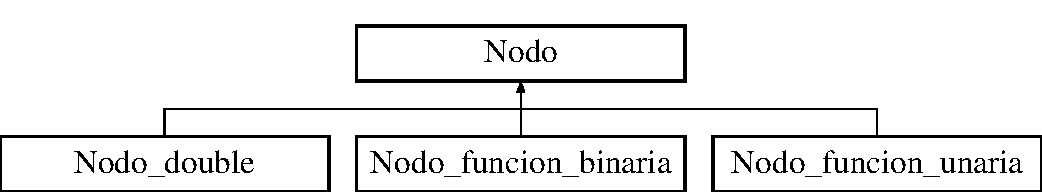
\includegraphics[height=2.000000cm]{class_nodo}
\end{center}
\end{figure}
\subsection*{Métodos públicos}
\begin{DoxyCompactItemize}
\item 
\hyperlink{class_nodo_ac30bd1bed827ef8784fd3cebd032e9a4}{Nodo} ()
\item 
virtual \hyperlink{class_nodo_a8a1dd01c95ff7bcb1182318498e834f9}{$\sim$\+Nodo} ()
\item 
virtual void \hyperlink{class_nodo_aaec6b546849827a198f8f9cfb785ddae}{set\+\_\+valor} ()
\item 
void \hyperlink{class_nodo_a1fdafb332912a0627e38f49e48c6c7a8}{agregar\+\_\+der} (\hyperlink{class_nodo}{Nodo} $\ast$)
\item 
void \hyperlink{class_nodo_ac40bf9aeb6268154ae64ba30808aead0}{agregar\+\_\+izq} (\hyperlink{class_nodo}{Nodo} $\ast$)
\item 
virtual void \hyperlink{class_nodo_af1d46c59678aad7bd2d772b0cea8d0b6}{get\+\_\+valor} (double $\ast$a)
\item 
virtual void \hyperlink{class_nodo_a391f7fb5f14e8c1ac8c0a54c158cf0db}{set\+\_\+valor} (double)
\item 
virtual void \hyperlink{class_nodo_a6b4c640c1cb52203a259321b4bb5ad17}{obtener\+\_\+variables} ()
\item 
virtual void \hyperlink{class_nodo_a0c4cf8fa55c25f9a4a9a68a0b07d9108}{get\+\_\+valor} (double($\ast$\&funcion)(double, double))
\item 
virtual void \hyperlink{class_nodo_af7b0ec4fc3a0a3ef46dc31eca99fdbd6}{set\+\_\+valor} (double($\ast$\&funcion)(double, double))
\item 
virtual void \hyperlink{class_nodo_a4bd234bb2194e7708e71f25d125b9934}{get\+\_\+valor} (double($\ast$\&funcion)(double))
\item 
virtual void \hyperlink{class_nodo_a134a6a0ca143bfa73bc6e8184bb9f69d}{set\+\_\+valor} (double($\ast$\&funcion)(double))
\item 
virtual double \hyperlink{class_nodo_a3f06904e422717bbc621acc054590755}{procesar} ()
\item 
void \hyperlink{class_nodo_aca274320e1051fe43ff5543140be2721}{verif\+\_\+variables} ()
\end{DoxyCompactItemize}
\subsection*{Atributos públicos}
\begin{DoxyCompactItemize}
\item 
\hyperlink{class_nodo}{Nodo} $\ast$ \hyperlink{class_nodo_a8e0d3bbd637491daad3716d8731881f7}{izq}
\item 
\hyperlink{class_nodo}{Nodo} $\ast$ \hyperlink{class_nodo_a9df44a5e283816852c24c43ebc1868dc}{der}
\item 
std\+::vector$<$ std\+::tuple$<$ std\+::string, double $\ast$ $>$ $>$ $\ast$ \hyperlink{class_nodo_afbf8312c82ff9a5b6194a6a252a1abae}{variables}
\end{DoxyCompactItemize}


\subsection{Documentación del constructor y destructor}
\index{Nodo@{Nodo}!Nodo@{Nodo}}
\index{Nodo@{Nodo}!Nodo@{Nodo}}
\subsubsection[{\texorpdfstring{Nodo()}{Nodo()}}]{\setlength{\rightskip}{0pt plus 5cm}Nodo\+::\+Nodo (
\begin{DoxyParamCaption}
{}
\end{DoxyParamCaption}
)}\hypertarget{class_nodo_ac30bd1bed827ef8784fd3cebd032e9a4}{}\label{class_nodo_ac30bd1bed827ef8784fd3cebd032e9a4}
\index{Nodo@{Nodo}!````~Nodo@{$\sim$\+Nodo}}
\index{````~Nodo@{$\sim$\+Nodo}!Nodo@{Nodo}}
\subsubsection[{\texorpdfstring{$\sim$\+Nodo()}{~Nodo()}}]{\setlength{\rightskip}{0pt plus 5cm}Nodo\+::$\sim$\+Nodo (
\begin{DoxyParamCaption}
{}
\end{DoxyParamCaption}
)\hspace{0.3cm}{\ttfamily [virtual]}}\hypertarget{class_nodo_a8a1dd01c95ff7bcb1182318498e834f9}{}\label{class_nodo_a8a1dd01c95ff7bcb1182318498e834f9}


\subsection{Documentación de las funciones miembro}
\index{Nodo@{Nodo}!agregar\+\_\+der@{agregar\+\_\+der}}
\index{agregar\+\_\+der@{agregar\+\_\+der}!Nodo@{Nodo}}
\subsubsection[{\texorpdfstring{agregar\+\_\+der(\+Nodo $\ast$)}{agregar_der(Nodo *)}}]{\setlength{\rightskip}{0pt plus 5cm}void Nodo\+::agregar\+\_\+der (
\begin{DoxyParamCaption}
\item[{{\bf Nodo} $\ast$}]{a}
\end{DoxyParamCaption}
)}\hypertarget{class_nodo_a1fdafb332912a0627e38f49e48c6c7a8}{}\label{class_nodo_a1fdafb332912a0627e38f49e48c6c7a8}
\index{Nodo@{Nodo}!agregar\+\_\+izq@{agregar\+\_\+izq}}
\index{agregar\+\_\+izq@{agregar\+\_\+izq}!Nodo@{Nodo}}
\subsubsection[{\texorpdfstring{agregar\+\_\+izq(\+Nodo $\ast$)}{agregar_izq(Nodo *)}}]{\setlength{\rightskip}{0pt plus 5cm}void Nodo\+::agregar\+\_\+izq (
\begin{DoxyParamCaption}
\item[{{\bf Nodo} $\ast$}]{a}
\end{DoxyParamCaption}
)}\hypertarget{class_nodo_ac40bf9aeb6268154ae64ba30808aead0}{}\label{class_nodo_ac40bf9aeb6268154ae64ba30808aead0}
\index{Nodo@{Nodo}!get\+\_\+valor@{get\+\_\+valor}}
\index{get\+\_\+valor@{get\+\_\+valor}!Nodo@{Nodo}}
\subsubsection[{\texorpdfstring{get\+\_\+valor(double $\ast$a)}{get_valor(double *a)}}]{\setlength{\rightskip}{0pt plus 5cm}virtual void Nodo\+::get\+\_\+valor (
\begin{DoxyParamCaption}
\item[{double $\ast$}]{a}
\end{DoxyParamCaption}
)\hspace{0.3cm}{\ttfamily [inline]}, {\ttfamily [virtual]}}\hypertarget{class_nodo_af1d46c59678aad7bd2d772b0cea8d0b6}{}\label{class_nodo_af1d46c59678aad7bd2d772b0cea8d0b6}


Reimplementado en \hyperlink{class_nodo__double_a4eb67c264f37c66d101d832ec981717b}{Nodo\+\_\+double}.

\index{Nodo@{Nodo}!get\+\_\+valor@{get\+\_\+valor}}
\index{get\+\_\+valor@{get\+\_\+valor}!Nodo@{Nodo}}
\subsubsection[{\texorpdfstring{get\+\_\+valor(double($\ast$\&funcion)(double, double))}{get_valor(double(*&funcion)(double, double))}}]{\setlength{\rightskip}{0pt plus 5cm}virtual void Nodo\+::get\+\_\+valor (
\begin{DoxyParamCaption}
\item[{double($\ast$\&)(double, double)}]{funcion}
\end{DoxyParamCaption}
)\hspace{0.3cm}{\ttfamily [inline]}, {\ttfamily [virtual]}}\hypertarget{class_nodo_a0c4cf8fa55c25f9a4a9a68a0b07d9108}{}\label{class_nodo_a0c4cf8fa55c25f9a4a9a68a0b07d9108}


Reimplementado en \hyperlink{class_nodo__funcion__binaria_ada34095260c6d6b9f8279edb6595db38}{Nodo\+\_\+funcion\+\_\+binaria}.

\index{Nodo@{Nodo}!get\+\_\+valor@{get\+\_\+valor}}
\index{get\+\_\+valor@{get\+\_\+valor}!Nodo@{Nodo}}
\subsubsection[{\texorpdfstring{get\+\_\+valor(double($\ast$\&funcion)(double))}{get_valor(double(*&funcion)(double))}}]{\setlength{\rightskip}{0pt plus 5cm}virtual void Nodo\+::get\+\_\+valor (
\begin{DoxyParamCaption}
\item[{double($\ast$\&)(double)}]{funcion}
\end{DoxyParamCaption}
)\hspace{0.3cm}{\ttfamily [inline]}, {\ttfamily [virtual]}}\hypertarget{class_nodo_a4bd234bb2194e7708e71f25d125b9934}{}\label{class_nodo_a4bd234bb2194e7708e71f25d125b9934}


Reimplementado en \hyperlink{class_nodo__funcion__unaria_ada80a2928510b76650aa2c336f9db8fa}{Nodo\+\_\+funcion\+\_\+unaria}.

\index{Nodo@{Nodo}!obtener\+\_\+variables@{obtener\+\_\+variables}}
\index{obtener\+\_\+variables@{obtener\+\_\+variables}!Nodo@{Nodo}}
\subsubsection[{\texorpdfstring{obtener\+\_\+variables()}{obtener_variables()}}]{\setlength{\rightskip}{0pt plus 5cm}virtual void Nodo\+::obtener\+\_\+variables (
\begin{DoxyParamCaption}
{}
\end{DoxyParamCaption}
)\hspace{0.3cm}{\ttfamily [inline]}, {\ttfamily [virtual]}}\hypertarget{class_nodo_a6b4c640c1cb52203a259321b4bb5ad17}{}\label{class_nodo_a6b4c640c1cb52203a259321b4bb5ad17}


Reimplementado en \hyperlink{class_nodo__double_a92a96c692af58eb4197ae64e085beb41}{Nodo\+\_\+double}, \hyperlink{class_nodo__funcion__binaria_a25ca9388d98b6ddbc950c2b9a2894645}{Nodo\+\_\+funcion\+\_\+binaria} y \hyperlink{class_nodo__funcion__unaria_a12bf4ec6430f11f4ffb4421a2f4af6f0}{Nodo\+\_\+funcion\+\_\+unaria}.

\index{Nodo@{Nodo}!procesar@{procesar}}
\index{procesar@{procesar}!Nodo@{Nodo}}
\subsubsection[{\texorpdfstring{procesar()}{procesar()}}]{\setlength{\rightskip}{0pt plus 5cm}virtual double Nodo\+::procesar (
\begin{DoxyParamCaption}
{}
\end{DoxyParamCaption}
)\hspace{0.3cm}{\ttfamily [inline]}, {\ttfamily [virtual]}}\hypertarget{class_nodo_a3f06904e422717bbc621acc054590755}{}\label{class_nodo_a3f06904e422717bbc621acc054590755}


Reimplementado en \hyperlink{class_nodo__funcion__binaria_a5637c538189912ddeb2b5f86a6855c0d}{Nodo\+\_\+funcion\+\_\+binaria}, \hyperlink{class_nodo__double_ac1062fd8a1c495f32b10be1a1e371748}{Nodo\+\_\+double} y \hyperlink{class_nodo__funcion__unaria_a1d6be00c52fad541beccf20bcf1a9122}{Nodo\+\_\+funcion\+\_\+unaria}.

\index{Nodo@{Nodo}!set\+\_\+valor@{set\+\_\+valor}}
\index{set\+\_\+valor@{set\+\_\+valor}!Nodo@{Nodo}}
\subsubsection[{\texorpdfstring{set\+\_\+valor()}{set_valor()}}]{\setlength{\rightskip}{0pt plus 5cm}virtual void Nodo\+::set\+\_\+valor (
\begin{DoxyParamCaption}
{}
\end{DoxyParamCaption}
)\hspace{0.3cm}{\ttfamily [inline]}, {\ttfamily [virtual]}}\hypertarget{class_nodo_aaec6b546849827a198f8f9cfb785ddae}{}\label{class_nodo_aaec6b546849827a198f8f9cfb785ddae}
\index{Nodo@{Nodo}!set\+\_\+valor@{set\+\_\+valor}}
\index{set\+\_\+valor@{set\+\_\+valor}!Nodo@{Nodo}}
\subsubsection[{\texorpdfstring{set\+\_\+valor(double)}{set_valor(double)}}]{\setlength{\rightskip}{0pt plus 5cm}virtual void Nodo\+::set\+\_\+valor (
\begin{DoxyParamCaption}
\item[{double}]{}
\end{DoxyParamCaption}
)\hspace{0.3cm}{\ttfamily [inline]}, {\ttfamily [virtual]}}\hypertarget{class_nodo_a391f7fb5f14e8c1ac8c0a54c158cf0db}{}\label{class_nodo_a391f7fb5f14e8c1ac8c0a54c158cf0db}


Reimplementado en \hyperlink{class_nodo__double_a46f39301fcb3971e1d452be7bdf6f35a}{Nodo\+\_\+double}.

\index{Nodo@{Nodo}!set\+\_\+valor@{set\+\_\+valor}}
\index{set\+\_\+valor@{set\+\_\+valor}!Nodo@{Nodo}}
\subsubsection[{\texorpdfstring{set\+\_\+valor(double($\ast$\&funcion)(double, double))}{set_valor(double(*&funcion)(double, double))}}]{\setlength{\rightskip}{0pt plus 5cm}virtual void Nodo\+::set\+\_\+valor (
\begin{DoxyParamCaption}
\item[{double($\ast$\&)(double, double)}]{funcion}
\end{DoxyParamCaption}
)\hspace{0.3cm}{\ttfamily [inline]}, {\ttfamily [virtual]}}\hypertarget{class_nodo_af7b0ec4fc3a0a3ef46dc31eca99fdbd6}{}\label{class_nodo_af7b0ec4fc3a0a3ef46dc31eca99fdbd6}


Reimplementado en \hyperlink{class_nodo__funcion__binaria_a07a097c0b959884106aed5b54d885c65}{Nodo\+\_\+funcion\+\_\+binaria}.

\index{Nodo@{Nodo}!set\+\_\+valor@{set\+\_\+valor}}
\index{set\+\_\+valor@{set\+\_\+valor}!Nodo@{Nodo}}
\subsubsection[{\texorpdfstring{set\+\_\+valor(double($\ast$\&funcion)(double))}{set_valor(double(*&funcion)(double))}}]{\setlength{\rightskip}{0pt plus 5cm}virtual void Nodo\+::set\+\_\+valor (
\begin{DoxyParamCaption}
\item[{double($\ast$\&)(double)}]{funcion}
\end{DoxyParamCaption}
)\hspace{0.3cm}{\ttfamily [inline]}, {\ttfamily [virtual]}}\hypertarget{class_nodo_a134a6a0ca143bfa73bc6e8184bb9f69d}{}\label{class_nodo_a134a6a0ca143bfa73bc6e8184bb9f69d}


Reimplementado en \hyperlink{class_nodo__funcion__unaria_a4634ffcf664c11c2cd5d4546c429476c}{Nodo\+\_\+funcion\+\_\+unaria}.

\index{Nodo@{Nodo}!verif\+\_\+variables@{verif\+\_\+variables}}
\index{verif\+\_\+variables@{verif\+\_\+variables}!Nodo@{Nodo}}
\subsubsection[{\texorpdfstring{verif\+\_\+variables()}{verif_variables()}}]{\setlength{\rightskip}{0pt plus 5cm}void Nodo\+::verif\+\_\+variables (
\begin{DoxyParamCaption}
{}
\end{DoxyParamCaption}
)}\hypertarget{class_nodo_aca274320e1051fe43ff5543140be2721}{}\label{class_nodo_aca274320e1051fe43ff5543140be2721}


\subsection{Documentación de los datos miembro}
\index{Nodo@{Nodo}!der@{der}}
\index{der@{der}!Nodo@{Nodo}}
\subsubsection[{\texorpdfstring{der}{der}}]{\setlength{\rightskip}{0pt plus 5cm}{\bf Nodo}$\ast$ Nodo\+::der}\hypertarget{class_nodo_a9df44a5e283816852c24c43ebc1868dc}{}\label{class_nodo_a9df44a5e283816852c24c43ebc1868dc}
\index{Nodo@{Nodo}!izq@{izq}}
\index{izq@{izq}!Nodo@{Nodo}}
\subsubsection[{\texorpdfstring{izq}{izq}}]{\setlength{\rightskip}{0pt plus 5cm}{\bf Nodo}$\ast$ Nodo\+::izq}\hypertarget{class_nodo_a8e0d3bbd637491daad3716d8731881f7}{}\label{class_nodo_a8e0d3bbd637491daad3716d8731881f7}
\index{Nodo@{Nodo}!variables@{variables}}
\index{variables@{variables}!Nodo@{Nodo}}
\subsubsection[{\texorpdfstring{variables}{variables}}]{\setlength{\rightskip}{0pt plus 5cm}std\+::vector$<$std\+::tuple$<$std\+::string,double$\ast$$>$ $>$$\ast$ Nodo\+::variables}\hypertarget{class_nodo_afbf8312c82ff9a5b6194a6a252a1abae}{}\label{class_nodo_afbf8312c82ff9a5b6194a6a252a1abae}


La documentación para esta clase fue generada a partir de los siguientes ficheros\+:\begin{DoxyCompactItemize}
\item 
Parser/include/\hyperlink{_nodo_8h}{Nodo.\+h}\item 
Parser/src/\hyperlink{_nodo_8cpp}{Nodo.\+cpp}\end{DoxyCompactItemize}

\hypertarget{class_nodo__double}{}\section{Referencia de la Clase Nodo\+\_\+double}
\label{class_nodo__double}\index{Nodo\+\_\+double@{Nodo\+\_\+double}}


{\ttfamily \#include $<$Nodo\+\_\+double.\+h$>$}

Diagrama de herencias de Nodo\+\_\+double\begin{figure}[H]
\begin{center}
\leavevmode
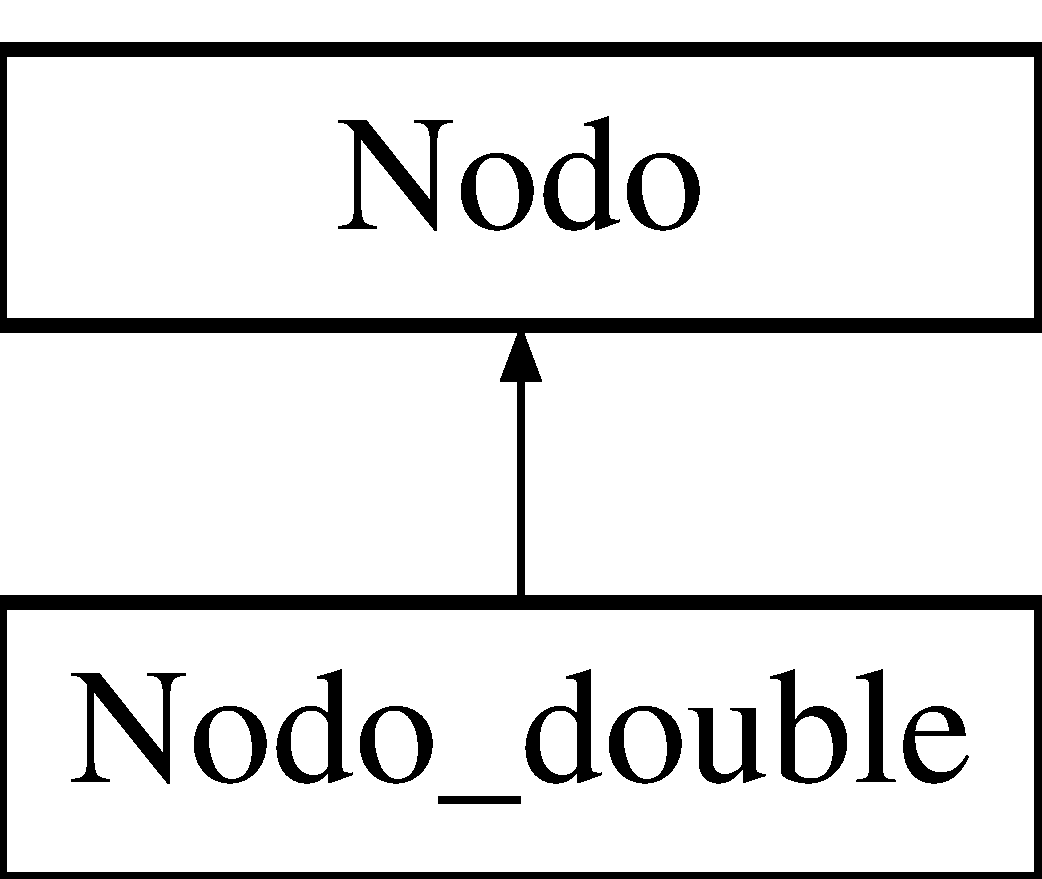
\includegraphics[height=2.000000cm]{class_nodo__double}
\end{center}
\end{figure}
\subsection*{Métodos públicos}
\begin{DoxyCompactItemize}
\item 
\hyperlink{class_nodo__double_a27c5b79400ab015339de2c5f898e81ce}{Nodo\+\_\+double} ()
\item 
\hyperlink{class_nodo__double_a165c997a53adf1f69e871da9e4bf8823}{Nodo\+\_\+double} (double a)
\item 
\hyperlink{class_nodo__double_af1e0ccdd5719def6ba57855bab6f1f81}{Nodo\+\_\+double} (std\+::string a)
\item 
virtual \hyperlink{class_nodo__double_a91facad1ce7ffef3ce80d5faff0016c5}{$\sim$\+Nodo\+\_\+double} ()
\item 
void \hyperlink{class_nodo__double_a4eb67c264f37c66d101d832ec981717b}{get\+\_\+valor} (double $\ast$)
\item 
void \hyperlink{class_nodo__double_a46f39301fcb3971e1d452be7bdf6f35a}{set\+\_\+valor} (double)
\item 
double \hyperlink{class_nodo__double_ac1062fd8a1c495f32b10be1a1e371748}{procesar} ()
\item 
void \hyperlink{class_nodo__double_a92a96c692af58eb4197ae64e085beb41}{obtener\+\_\+variables} ()
\end{DoxyCompactItemize}
\subsection*{Atributos públicos}
\begin{DoxyCompactItemize}
\item 
double $\ast$ \hyperlink{class_nodo__double_a8a9a0dc98d04e88ca67d517efb9764df}{valor}
\end{DoxyCompactItemize}


\subsection{Documentación del constructor y destructor}
\index{Nodo\+\_\+double@{Nodo\+\_\+double}!Nodo\+\_\+double@{Nodo\+\_\+double}}
\index{Nodo\+\_\+double@{Nodo\+\_\+double}!Nodo\+\_\+double@{Nodo\+\_\+double}}
\subsubsection[{\texorpdfstring{Nodo\+\_\+double()}{Nodo_double()}}]{\setlength{\rightskip}{0pt plus 5cm}Nodo\+\_\+double\+::\+Nodo\+\_\+double (
\begin{DoxyParamCaption}
{}
\end{DoxyParamCaption}
)}\hypertarget{class_nodo__double_a27c5b79400ab015339de2c5f898e81ce}{}\label{class_nodo__double_a27c5b79400ab015339de2c5f898e81ce}
\index{Nodo\+\_\+double@{Nodo\+\_\+double}!Nodo\+\_\+double@{Nodo\+\_\+double}}
\index{Nodo\+\_\+double@{Nodo\+\_\+double}!Nodo\+\_\+double@{Nodo\+\_\+double}}
\subsubsection[{\texorpdfstring{Nodo\+\_\+double(double a)}{Nodo_double(double a)}}]{\setlength{\rightskip}{0pt plus 5cm}Nodo\+\_\+double\+::\+Nodo\+\_\+double (
\begin{DoxyParamCaption}
\item[{double}]{a}
\end{DoxyParamCaption}
)\hspace{0.3cm}{\ttfamily [inline]}}\hypertarget{class_nodo__double_a165c997a53adf1f69e871da9e4bf8823}{}\label{class_nodo__double_a165c997a53adf1f69e871da9e4bf8823}
\index{Nodo\+\_\+double@{Nodo\+\_\+double}!Nodo\+\_\+double@{Nodo\+\_\+double}}
\index{Nodo\+\_\+double@{Nodo\+\_\+double}!Nodo\+\_\+double@{Nodo\+\_\+double}}
\subsubsection[{\texorpdfstring{Nodo\+\_\+double(std\+::string a)}{Nodo_double(std::string a)}}]{\setlength{\rightskip}{0pt plus 5cm}Nodo\+\_\+double\+::\+Nodo\+\_\+double (
\begin{DoxyParamCaption}
\item[{std\+::string}]{a}
\end{DoxyParamCaption}
)}\hypertarget{class_nodo__double_af1e0ccdd5719def6ba57855bab6f1f81}{}\label{class_nodo__double_af1e0ccdd5719def6ba57855bab6f1f81}
\index{Nodo\+\_\+double@{Nodo\+\_\+double}!````~Nodo\+\_\+double@{$\sim$\+Nodo\+\_\+double}}
\index{````~Nodo\+\_\+double@{$\sim$\+Nodo\+\_\+double}!Nodo\+\_\+double@{Nodo\+\_\+double}}
\subsubsection[{\texorpdfstring{$\sim$\+Nodo\+\_\+double()}{~Nodo_double()}}]{\setlength{\rightskip}{0pt plus 5cm}Nodo\+\_\+double\+::$\sim$\+Nodo\+\_\+double (
\begin{DoxyParamCaption}
{}
\end{DoxyParamCaption}
)\hspace{0.3cm}{\ttfamily [virtual]}}\hypertarget{class_nodo__double_a91facad1ce7ffef3ce80d5faff0016c5}{}\label{class_nodo__double_a91facad1ce7ffef3ce80d5faff0016c5}


\subsection{Documentación de las funciones miembro}
\index{Nodo\+\_\+double@{Nodo\+\_\+double}!get\+\_\+valor@{get\+\_\+valor}}
\index{get\+\_\+valor@{get\+\_\+valor}!Nodo\+\_\+double@{Nodo\+\_\+double}}
\subsubsection[{\texorpdfstring{get\+\_\+valor(double $\ast$)}{get_valor(double *)}}]{\setlength{\rightskip}{0pt plus 5cm}void Nodo\+\_\+double\+::get\+\_\+valor (
\begin{DoxyParamCaption}
\item[{double $\ast$}]{a}
\end{DoxyParamCaption}
)\hspace{0.3cm}{\ttfamily [virtual]}}\hypertarget{class_nodo__double_a4eb67c264f37c66d101d832ec981717b}{}\label{class_nodo__double_a4eb67c264f37c66d101d832ec981717b}


Reimplementado de \hyperlink{class_nodo_af1d46c59678aad7bd2d772b0cea8d0b6}{Nodo}.

\index{Nodo\+\_\+double@{Nodo\+\_\+double}!obtener\+\_\+variables@{obtener\+\_\+variables}}
\index{obtener\+\_\+variables@{obtener\+\_\+variables}!Nodo\+\_\+double@{Nodo\+\_\+double}}
\subsubsection[{\texorpdfstring{obtener\+\_\+variables()}{obtener_variables()}}]{\setlength{\rightskip}{0pt plus 5cm}void Nodo\+\_\+double\+::obtener\+\_\+variables (
\begin{DoxyParamCaption}
{}
\end{DoxyParamCaption}
)\hspace{0.3cm}{\ttfamily [virtual]}}\hypertarget{class_nodo__double_a92a96c692af58eb4197ae64e085beb41}{}\label{class_nodo__double_a92a96c692af58eb4197ae64e085beb41}


Reimplementado de \hyperlink{class_nodo_a6b4c640c1cb52203a259321b4bb5ad17}{Nodo}.

\index{Nodo\+\_\+double@{Nodo\+\_\+double}!procesar@{procesar}}
\index{procesar@{procesar}!Nodo\+\_\+double@{Nodo\+\_\+double}}
\subsubsection[{\texorpdfstring{procesar()}{procesar()}}]{\setlength{\rightskip}{0pt plus 5cm}double Nodo\+\_\+double\+::procesar (
\begin{DoxyParamCaption}
{}
\end{DoxyParamCaption}
)\hspace{0.3cm}{\ttfamily [virtual]}}\hypertarget{class_nodo__double_ac1062fd8a1c495f32b10be1a1e371748}{}\label{class_nodo__double_ac1062fd8a1c495f32b10be1a1e371748}


Reimplementado de \hyperlink{class_nodo_a3f06904e422717bbc621acc054590755}{Nodo}.

\index{Nodo\+\_\+double@{Nodo\+\_\+double}!set\+\_\+valor@{set\+\_\+valor}}
\index{set\+\_\+valor@{set\+\_\+valor}!Nodo\+\_\+double@{Nodo\+\_\+double}}
\subsubsection[{\texorpdfstring{set\+\_\+valor(double)}{set_valor(double)}}]{\setlength{\rightskip}{0pt plus 5cm}void Nodo\+\_\+double\+::set\+\_\+valor (
\begin{DoxyParamCaption}
\item[{double}]{a}
\end{DoxyParamCaption}
)\hspace{0.3cm}{\ttfamily [virtual]}}\hypertarget{class_nodo__double_a46f39301fcb3971e1d452be7bdf6f35a}{}\label{class_nodo__double_a46f39301fcb3971e1d452be7bdf6f35a}


Reimplementado de \hyperlink{class_nodo_a391f7fb5f14e8c1ac8c0a54c158cf0db}{Nodo}.



\subsection{Documentación de los datos miembro}
\index{Nodo\+\_\+double@{Nodo\+\_\+double}!valor@{valor}}
\index{valor@{valor}!Nodo\+\_\+double@{Nodo\+\_\+double}}
\subsubsection[{\texorpdfstring{valor}{valor}}]{\setlength{\rightskip}{0pt plus 5cm}double$\ast$ Nodo\+\_\+double\+::valor}\hypertarget{class_nodo__double_a8a9a0dc98d04e88ca67d517efb9764df}{}\label{class_nodo__double_a8a9a0dc98d04e88ca67d517efb9764df}


La documentación para esta clase fue generada a partir de los siguientes ficheros\+:\begin{DoxyCompactItemize}
\item 
Parser/include/\hyperlink{_nodo__double_8h}{Nodo\+\_\+double.\+h}\item 
Parser/src/\hyperlink{_nodo__double_8cpp}{Nodo\+\_\+double.\+cpp}\end{DoxyCompactItemize}

\hypertarget{class_nodo__funcion__binaria}{}\section{Referencia de la Clase Nodo\+\_\+funcion\+\_\+binaria}
\label{class_nodo__funcion__binaria}\index{Nodo\+\_\+funcion\+\_\+binaria@{Nodo\+\_\+funcion\+\_\+binaria}}


{\ttfamily \#include $<$Nodo\+\_\+funcion\+\_\+binaria.\+h$>$}

Diagrama de herencias de Nodo\+\_\+funcion\+\_\+binaria\begin{figure}[H]
\begin{center}
\leavevmode
\includegraphics[height=2.000000cm]{class_nodo__funcion__binaria}
\end{center}
\end{figure}
\subsection*{Métodos públicos}
\begin{DoxyCompactItemize}
\item 
\hyperlink{class_nodo__funcion__binaria_a2759485f81a0b5eecb4344e708a05e7f}{Nodo\+\_\+funcion\+\_\+binaria} ()
\item 
\hyperlink{class_nodo__funcion__binaria_a03cad31c73d5d42d60ba4252861ba56e}{Nodo\+\_\+funcion\+\_\+binaria} (double(\&funcion)(double, double))
\item 
void \hyperlink{class_nodo__funcion__binaria_ada34095260c6d6b9f8279edb6595db38}{get\+\_\+valor} (double($\ast$\&funcion)(double, double))
\item 
void \hyperlink{class_nodo__funcion__binaria_a07a097c0b959884106aed5b54d885c65}{set\+\_\+valor} (double($\ast$\&funcion)(double, double))
\item 
void \hyperlink{class_nodo__funcion__binaria_a25ca9388d98b6ddbc950c2b9a2894645}{obtener\+\_\+variables} ()
\item 
virtual \hyperlink{class_nodo__funcion__binaria_a88950c2b54d834ffd3a86f982e7bc3d7}{$\sim$\+Nodo\+\_\+funcion\+\_\+binaria} ()
\item 
double \hyperlink{class_nodo__funcion__binaria_a5637c538189912ddeb2b5f86a6855c0d}{procesar} ()
\end{DoxyCompactItemize}
\subsection*{Atributos públicos}
\begin{DoxyCompactItemize}
\item 
double($\ast$ \hyperlink{class_nodo__funcion__binaria_a1ec2b5d955b3c91bc1cc56447d9d9034}{valor} )(double, double)
\end{DoxyCompactItemize}


\subsection{Documentación del constructor y destructor}
\index{Nodo\+\_\+funcion\+\_\+binaria@{Nodo\+\_\+funcion\+\_\+binaria}!Nodo\+\_\+funcion\+\_\+binaria@{Nodo\+\_\+funcion\+\_\+binaria}}
\index{Nodo\+\_\+funcion\+\_\+binaria@{Nodo\+\_\+funcion\+\_\+binaria}!Nodo\+\_\+funcion\+\_\+binaria@{Nodo\+\_\+funcion\+\_\+binaria}}
\subsubsection[{\texorpdfstring{Nodo\+\_\+funcion\+\_\+binaria()}{Nodo_funcion_binaria()}}]{\setlength{\rightskip}{0pt plus 5cm}Nodo\+\_\+funcion\+\_\+binaria\+::\+Nodo\+\_\+funcion\+\_\+binaria (
\begin{DoxyParamCaption}
{}
\end{DoxyParamCaption}
)}\hypertarget{class_nodo__funcion__binaria_a2759485f81a0b5eecb4344e708a05e7f}{}\label{class_nodo__funcion__binaria_a2759485f81a0b5eecb4344e708a05e7f}
\index{Nodo\+\_\+funcion\+\_\+binaria@{Nodo\+\_\+funcion\+\_\+binaria}!Nodo\+\_\+funcion\+\_\+binaria@{Nodo\+\_\+funcion\+\_\+binaria}}
\index{Nodo\+\_\+funcion\+\_\+binaria@{Nodo\+\_\+funcion\+\_\+binaria}!Nodo\+\_\+funcion\+\_\+binaria@{Nodo\+\_\+funcion\+\_\+binaria}}
\subsubsection[{\texorpdfstring{Nodo\+\_\+funcion\+\_\+binaria(double(\&funcion)(double, double))}{Nodo_funcion_binaria(double(&funcion)(double, double))}}]{\setlength{\rightskip}{0pt plus 5cm}Nodo\+\_\+funcion\+\_\+binaria\+::\+Nodo\+\_\+funcion\+\_\+binaria (
\begin{DoxyParamCaption}
\item[{double(\&)(double, double)}]{funcion}
\end{DoxyParamCaption}
)\hspace{0.3cm}{\ttfamily [inline]}}\hypertarget{class_nodo__funcion__binaria_a03cad31c73d5d42d60ba4252861ba56e}{}\label{class_nodo__funcion__binaria_a03cad31c73d5d42d60ba4252861ba56e}
\index{Nodo\+\_\+funcion\+\_\+binaria@{Nodo\+\_\+funcion\+\_\+binaria}!````~Nodo\+\_\+funcion\+\_\+binaria@{$\sim$\+Nodo\+\_\+funcion\+\_\+binaria}}
\index{````~Nodo\+\_\+funcion\+\_\+binaria@{$\sim$\+Nodo\+\_\+funcion\+\_\+binaria}!Nodo\+\_\+funcion\+\_\+binaria@{Nodo\+\_\+funcion\+\_\+binaria}}
\subsubsection[{\texorpdfstring{$\sim$\+Nodo\+\_\+funcion\+\_\+binaria()}{~Nodo_funcion_binaria()}}]{\setlength{\rightskip}{0pt plus 5cm}Nodo\+\_\+funcion\+\_\+binaria\+::$\sim$\+Nodo\+\_\+funcion\+\_\+binaria (
\begin{DoxyParamCaption}
{}
\end{DoxyParamCaption}
)\hspace{0.3cm}{\ttfamily [virtual]}}\hypertarget{class_nodo__funcion__binaria_a88950c2b54d834ffd3a86f982e7bc3d7}{}\label{class_nodo__funcion__binaria_a88950c2b54d834ffd3a86f982e7bc3d7}


\subsection{Documentación de las funciones miembro}
\index{Nodo\+\_\+funcion\+\_\+binaria@{Nodo\+\_\+funcion\+\_\+binaria}!get\+\_\+valor@{get\+\_\+valor}}
\index{get\+\_\+valor@{get\+\_\+valor}!Nodo\+\_\+funcion\+\_\+binaria@{Nodo\+\_\+funcion\+\_\+binaria}}
\subsubsection[{\texorpdfstring{get\+\_\+valor(double($\ast$\&funcion)(double, double))}{get_valor(double(*&funcion)(double, double))}}]{\setlength{\rightskip}{0pt plus 5cm}void Nodo\+\_\+funcion\+\_\+binaria\+::get\+\_\+valor (
\begin{DoxyParamCaption}
\item[{double($\ast$\&)(double, double)}]{funcion}
\end{DoxyParamCaption}
)\hspace{0.3cm}{\ttfamily [virtual]}}\hypertarget{class_nodo__funcion__binaria_ada34095260c6d6b9f8279edb6595db38}{}\label{class_nodo__funcion__binaria_ada34095260c6d6b9f8279edb6595db38}


Reimplementado de \hyperlink{class_nodo_a0c4cf8fa55c25f9a4a9a68a0b07d9108}{Nodo}.

\index{Nodo\+\_\+funcion\+\_\+binaria@{Nodo\+\_\+funcion\+\_\+binaria}!obtener\+\_\+variables@{obtener\+\_\+variables}}
\index{obtener\+\_\+variables@{obtener\+\_\+variables}!Nodo\+\_\+funcion\+\_\+binaria@{Nodo\+\_\+funcion\+\_\+binaria}}
\subsubsection[{\texorpdfstring{obtener\+\_\+variables()}{obtener_variables()}}]{\setlength{\rightskip}{0pt plus 5cm}void Nodo\+\_\+funcion\+\_\+binaria\+::obtener\+\_\+variables (
\begin{DoxyParamCaption}
{}
\end{DoxyParamCaption}
)\hspace{0.3cm}{\ttfamily [virtual]}}\hypertarget{class_nodo__funcion__binaria_a25ca9388d98b6ddbc950c2b9a2894645}{}\label{class_nodo__funcion__binaria_a25ca9388d98b6ddbc950c2b9a2894645}


Reimplementado de \hyperlink{class_nodo_a6b4c640c1cb52203a259321b4bb5ad17}{Nodo}.

\index{Nodo\+\_\+funcion\+\_\+binaria@{Nodo\+\_\+funcion\+\_\+binaria}!procesar@{procesar}}
\index{procesar@{procesar}!Nodo\+\_\+funcion\+\_\+binaria@{Nodo\+\_\+funcion\+\_\+binaria}}
\subsubsection[{\texorpdfstring{procesar()}{procesar()}}]{\setlength{\rightskip}{0pt plus 5cm}double Nodo\+\_\+funcion\+\_\+binaria\+::procesar (
\begin{DoxyParamCaption}
{}
\end{DoxyParamCaption}
)\hspace{0.3cm}{\ttfamily [virtual]}}\hypertarget{class_nodo__funcion__binaria_a5637c538189912ddeb2b5f86a6855c0d}{}\label{class_nodo__funcion__binaria_a5637c538189912ddeb2b5f86a6855c0d}


Reimplementado de \hyperlink{class_nodo_a3f06904e422717bbc621acc054590755}{Nodo}.

\index{Nodo\+\_\+funcion\+\_\+binaria@{Nodo\+\_\+funcion\+\_\+binaria}!set\+\_\+valor@{set\+\_\+valor}}
\index{set\+\_\+valor@{set\+\_\+valor}!Nodo\+\_\+funcion\+\_\+binaria@{Nodo\+\_\+funcion\+\_\+binaria}}
\subsubsection[{\texorpdfstring{set\+\_\+valor(double($\ast$\&funcion)(double, double))}{set_valor(double(*&funcion)(double, double))}}]{\setlength{\rightskip}{0pt plus 5cm}void Nodo\+\_\+funcion\+\_\+binaria\+::set\+\_\+valor (
\begin{DoxyParamCaption}
\item[{double($\ast$\&)(double, double)}]{funcion}
\end{DoxyParamCaption}
)\hspace{0.3cm}{\ttfamily [virtual]}}\hypertarget{class_nodo__funcion__binaria_a07a097c0b959884106aed5b54d885c65}{}\label{class_nodo__funcion__binaria_a07a097c0b959884106aed5b54d885c65}


Reimplementado de \hyperlink{class_nodo_af7b0ec4fc3a0a3ef46dc31eca99fdbd6}{Nodo}.



\subsection{Documentación de los datos miembro}
\index{Nodo\+\_\+funcion\+\_\+binaria@{Nodo\+\_\+funcion\+\_\+binaria}!valor@{valor}}
\index{valor@{valor}!Nodo\+\_\+funcion\+\_\+binaria@{Nodo\+\_\+funcion\+\_\+binaria}}
\subsubsection[{\texorpdfstring{valor}{valor}}]{\setlength{\rightskip}{0pt plus 5cm}double($\ast$ Nodo\+\_\+funcion\+\_\+binaria\+::valor) (double, double)}\hypertarget{class_nodo__funcion__binaria_a1ec2b5d955b3c91bc1cc56447d9d9034}{}\label{class_nodo__funcion__binaria_a1ec2b5d955b3c91bc1cc56447d9d9034}


La documentación para esta clase fue generada a partir de los siguientes ficheros\+:\begin{DoxyCompactItemize}
\item 
Parser/include/\hyperlink{_nodo__funcion__binaria_8h}{Nodo\+\_\+funcion\+\_\+binaria.\+h}\item 
Parser/src/\hyperlink{_nodo__funcion__binaria_8cpp}{Nodo\+\_\+funcion\+\_\+binaria.\+cpp}\end{DoxyCompactItemize}

\hypertarget{class_nodo__funcion__unaria}{}\section{Referencia de la Clase Nodo\+\_\+funcion\+\_\+unaria}
\label{class_nodo__funcion__unaria}\index{Nodo\+\_\+funcion\+\_\+unaria@{Nodo\+\_\+funcion\+\_\+unaria}}


{\ttfamily \#include $<$Nodo\+\_\+funcion\+\_\+unaria.\+h$>$}

Diagrama de herencias de Nodo\+\_\+funcion\+\_\+unaria\begin{figure}[H]
\begin{center}
\leavevmode
\includegraphics[height=2.000000cm]{class_nodo__funcion__unaria}
\end{center}
\end{figure}
\subsection*{Métodos públicos}
\begin{DoxyCompactItemize}
\item 
\hyperlink{class_nodo__funcion__unaria_ad8b8270d7c2bcdefbd7fe8ec0a2ad660}{Nodo\+\_\+funcion\+\_\+unaria} ()
\item 
\hyperlink{class_nodo__funcion__unaria_aae3c3384f4214e8c21b992894228023e}{Nodo\+\_\+funcion\+\_\+unaria} (double(\&funcion)(double))
\item 
void \hyperlink{class_nodo__funcion__unaria_ada80a2928510b76650aa2c336f9db8fa}{get\+\_\+valor} (double($\ast$\&funcion)(double))
\item 
void \hyperlink{class_nodo__funcion__unaria_a4634ffcf664c11c2cd5d4546c429476c}{set\+\_\+valor} (double($\ast$\&funcion)(double))
\item 
double \hyperlink{class_nodo__funcion__unaria_a1d6be00c52fad541beccf20bcf1a9122}{procesar} ()
\item 
void \hyperlink{class_nodo__funcion__unaria_a12bf4ec6430f11f4ffb4421a2f4af6f0}{obtener\+\_\+variables} ()
\item 
virtual \hyperlink{class_nodo__funcion__unaria_abd0b606fe115658eded2e1b65c2a94b5}{$\sim$\+Nodo\+\_\+funcion\+\_\+unaria} ()
\end{DoxyCompactItemize}
\subsection*{Atributos públicos}
\begin{DoxyCompactItemize}
\item 
double($\ast$ \hyperlink{class_nodo__funcion__unaria_ab9407e53aabe85b4c725b82a1f4a25be}{valor} )(double)
\end{DoxyCompactItemize}


\subsection{Documentación del constructor y destructor}
\index{Nodo\+\_\+funcion\+\_\+unaria@{Nodo\+\_\+funcion\+\_\+unaria}!Nodo\+\_\+funcion\+\_\+unaria@{Nodo\+\_\+funcion\+\_\+unaria}}
\index{Nodo\+\_\+funcion\+\_\+unaria@{Nodo\+\_\+funcion\+\_\+unaria}!Nodo\+\_\+funcion\+\_\+unaria@{Nodo\+\_\+funcion\+\_\+unaria}}
\subsubsection[{\texorpdfstring{Nodo\+\_\+funcion\+\_\+unaria()}{Nodo_funcion_unaria()}}]{\setlength{\rightskip}{0pt plus 5cm}Nodo\+\_\+funcion\+\_\+unaria\+::\+Nodo\+\_\+funcion\+\_\+unaria (
\begin{DoxyParamCaption}
{}
\end{DoxyParamCaption}
)}\hypertarget{class_nodo__funcion__unaria_ad8b8270d7c2bcdefbd7fe8ec0a2ad660}{}\label{class_nodo__funcion__unaria_ad8b8270d7c2bcdefbd7fe8ec0a2ad660}
\index{Nodo\+\_\+funcion\+\_\+unaria@{Nodo\+\_\+funcion\+\_\+unaria}!Nodo\+\_\+funcion\+\_\+unaria@{Nodo\+\_\+funcion\+\_\+unaria}}
\index{Nodo\+\_\+funcion\+\_\+unaria@{Nodo\+\_\+funcion\+\_\+unaria}!Nodo\+\_\+funcion\+\_\+unaria@{Nodo\+\_\+funcion\+\_\+unaria}}
\subsubsection[{\texorpdfstring{Nodo\+\_\+funcion\+\_\+unaria(double(\&funcion)(double))}{Nodo_funcion_unaria(double(&funcion)(double))}}]{\setlength{\rightskip}{0pt plus 5cm}Nodo\+\_\+funcion\+\_\+unaria\+::\+Nodo\+\_\+funcion\+\_\+unaria (
\begin{DoxyParamCaption}
\item[{double(\&)(double)}]{funcion}
\end{DoxyParamCaption}
)\hspace{0.3cm}{\ttfamily [inline]}}\hypertarget{class_nodo__funcion__unaria_aae3c3384f4214e8c21b992894228023e}{}\label{class_nodo__funcion__unaria_aae3c3384f4214e8c21b992894228023e}
\index{Nodo\+\_\+funcion\+\_\+unaria@{Nodo\+\_\+funcion\+\_\+unaria}!````~Nodo\+\_\+funcion\+\_\+unaria@{$\sim$\+Nodo\+\_\+funcion\+\_\+unaria}}
\index{````~Nodo\+\_\+funcion\+\_\+unaria@{$\sim$\+Nodo\+\_\+funcion\+\_\+unaria}!Nodo\+\_\+funcion\+\_\+unaria@{Nodo\+\_\+funcion\+\_\+unaria}}
\subsubsection[{\texorpdfstring{$\sim$\+Nodo\+\_\+funcion\+\_\+unaria()}{~Nodo_funcion_unaria()}}]{\setlength{\rightskip}{0pt plus 5cm}Nodo\+\_\+funcion\+\_\+unaria\+::$\sim$\+Nodo\+\_\+funcion\+\_\+unaria (
\begin{DoxyParamCaption}
{}
\end{DoxyParamCaption}
)\hspace{0.3cm}{\ttfamily [virtual]}}\hypertarget{class_nodo__funcion__unaria_abd0b606fe115658eded2e1b65c2a94b5}{}\label{class_nodo__funcion__unaria_abd0b606fe115658eded2e1b65c2a94b5}


\subsection{Documentación de las funciones miembro}
\index{Nodo\+\_\+funcion\+\_\+unaria@{Nodo\+\_\+funcion\+\_\+unaria}!get\+\_\+valor@{get\+\_\+valor}}
\index{get\+\_\+valor@{get\+\_\+valor}!Nodo\+\_\+funcion\+\_\+unaria@{Nodo\+\_\+funcion\+\_\+unaria}}
\subsubsection[{\texorpdfstring{get\+\_\+valor(double($\ast$\&funcion)(double))}{get_valor(double(*&funcion)(double))}}]{\setlength{\rightskip}{0pt plus 5cm}void Nodo\+\_\+funcion\+\_\+unaria\+::get\+\_\+valor (
\begin{DoxyParamCaption}
\item[{double($\ast$\&)(double)}]{funcion}
\end{DoxyParamCaption}
)\hspace{0.3cm}{\ttfamily [virtual]}}\hypertarget{class_nodo__funcion__unaria_ada80a2928510b76650aa2c336f9db8fa}{}\label{class_nodo__funcion__unaria_ada80a2928510b76650aa2c336f9db8fa}


Reimplementado de \hyperlink{class_nodo_a4bd234bb2194e7708e71f25d125b9934}{Nodo}.

\index{Nodo\+\_\+funcion\+\_\+unaria@{Nodo\+\_\+funcion\+\_\+unaria}!obtener\+\_\+variables@{obtener\+\_\+variables}}
\index{obtener\+\_\+variables@{obtener\+\_\+variables}!Nodo\+\_\+funcion\+\_\+unaria@{Nodo\+\_\+funcion\+\_\+unaria}}
\subsubsection[{\texorpdfstring{obtener\+\_\+variables()}{obtener_variables()}}]{\setlength{\rightskip}{0pt plus 5cm}void Nodo\+\_\+funcion\+\_\+unaria\+::obtener\+\_\+variables (
\begin{DoxyParamCaption}
{}
\end{DoxyParamCaption}
)\hspace{0.3cm}{\ttfamily [virtual]}}\hypertarget{class_nodo__funcion__unaria_a12bf4ec6430f11f4ffb4421a2f4af6f0}{}\label{class_nodo__funcion__unaria_a12bf4ec6430f11f4ffb4421a2f4af6f0}


Reimplementado de \hyperlink{class_nodo_a6b4c640c1cb52203a259321b4bb5ad17}{Nodo}.

\index{Nodo\+\_\+funcion\+\_\+unaria@{Nodo\+\_\+funcion\+\_\+unaria}!procesar@{procesar}}
\index{procesar@{procesar}!Nodo\+\_\+funcion\+\_\+unaria@{Nodo\+\_\+funcion\+\_\+unaria}}
\subsubsection[{\texorpdfstring{procesar()}{procesar()}}]{\setlength{\rightskip}{0pt plus 5cm}double Nodo\+\_\+funcion\+\_\+unaria\+::procesar (
\begin{DoxyParamCaption}
{}
\end{DoxyParamCaption}
)\hspace{0.3cm}{\ttfamily [virtual]}}\hypertarget{class_nodo__funcion__unaria_a1d6be00c52fad541beccf20bcf1a9122}{}\label{class_nodo__funcion__unaria_a1d6be00c52fad541beccf20bcf1a9122}


Reimplementado de \hyperlink{class_nodo_a3f06904e422717bbc621acc054590755}{Nodo}.

\index{Nodo\+\_\+funcion\+\_\+unaria@{Nodo\+\_\+funcion\+\_\+unaria}!set\+\_\+valor@{set\+\_\+valor}}
\index{set\+\_\+valor@{set\+\_\+valor}!Nodo\+\_\+funcion\+\_\+unaria@{Nodo\+\_\+funcion\+\_\+unaria}}
\subsubsection[{\texorpdfstring{set\+\_\+valor(double($\ast$\&funcion)(double))}{set_valor(double(*&funcion)(double))}}]{\setlength{\rightskip}{0pt plus 5cm}void Nodo\+\_\+funcion\+\_\+unaria\+::set\+\_\+valor (
\begin{DoxyParamCaption}
\item[{double($\ast$\&)(double)}]{funcion}
\end{DoxyParamCaption}
)\hspace{0.3cm}{\ttfamily [virtual]}}\hypertarget{class_nodo__funcion__unaria_a4634ffcf664c11c2cd5d4546c429476c}{}\label{class_nodo__funcion__unaria_a4634ffcf664c11c2cd5d4546c429476c}


Reimplementado de \hyperlink{class_nodo_a134a6a0ca143bfa73bc6e8184bb9f69d}{Nodo}.



\subsection{Documentación de los datos miembro}
\index{Nodo\+\_\+funcion\+\_\+unaria@{Nodo\+\_\+funcion\+\_\+unaria}!valor@{valor}}
\index{valor@{valor}!Nodo\+\_\+funcion\+\_\+unaria@{Nodo\+\_\+funcion\+\_\+unaria}}
\subsubsection[{\texorpdfstring{valor}{valor}}]{\setlength{\rightskip}{0pt plus 5cm}double($\ast$ Nodo\+\_\+funcion\+\_\+unaria\+::valor) (double)}\hypertarget{class_nodo__funcion__unaria_ab9407e53aabe85b4c725b82a1f4a25be}{}\label{class_nodo__funcion__unaria_ab9407e53aabe85b4c725b82a1f4a25be}


La documentación para esta clase fue generada a partir de los siguientes ficheros\+:\begin{DoxyCompactItemize}
\item 
Parser/include/\hyperlink{_nodo__funcion__unaria_8h}{Nodo\+\_\+funcion\+\_\+unaria.\+h}\item 
Parser/src/\hyperlink{_nodo__funcion__unaria_8cpp}{Nodo\+\_\+funcion\+\_\+unaria.\+cpp}\end{DoxyCompactItemize}

\hypertarget{classmu_1_1_parser}{}\section{Referencia de la Clase mu\+:\+:Parser}
\label{classmu_1_1_parser}\index{mu\+::\+Parser@{mu\+::\+Parser}}


Mathematical expressions parser.  




{\ttfamily \#include $<$mu\+Parser.\+h$>$}

Diagrama de herencias de mu\+:\+:Parser\begin{figure}[H]
\begin{center}
\leavevmode
\includegraphics[height=2.000000cm]{classmu_1_1_parser}
\end{center}
\end{figure}
\subsection*{Métodos públicos}
\begin{DoxyCompactItemize}
\item 
\hyperlink{classmu_1_1_parser_a76747bbf8c232e488e15f846e1b4ed34}{Parser} ()
\begin{DoxyCompactList}\small\item\em Constructor. \end{DoxyCompactList}\item 
virtual void \hyperlink{classmu_1_1_parser_a3279e2cf701ba8c2f850f5826a147f75}{Init\+Char\+Sets} ()
\begin{DoxyCompactList}\small\item\em Define the character sets. \end{DoxyCompactList}\item 
virtual void \hyperlink{classmu_1_1_parser_a9da582fd5385acfd97ec99a8790f8c6d}{Init\+Fun} ()
\begin{DoxyCompactList}\small\item\em Initialize the default functions. \end{DoxyCompactList}\item 
virtual void \hyperlink{classmu_1_1_parser_aefd1da7ba62d20d7276b1e70c8cb6a02}{Init\+Const} ()
\begin{DoxyCompactList}\small\item\em Initialize constants. \end{DoxyCompactList}\item 
virtual void \hyperlink{classmu_1_1_parser_a4ed9bdd0565bd57325bc49c12cf73e06}{Init\+Oprt} ()
\begin{DoxyCompactList}\small\item\em Initialize operators. \end{DoxyCompactList}\item 
virtual void \hyperlink{classmu_1_1_parser_a8e5afdde87b9f8acabde693441d4798c}{On\+Detect\+Var} (\hyperlink{namespacemu_ae9f8b44d9a97dd397180891e8390c3e9}{string\+\_\+type} $\ast$p\+Expr, int \&n\+Start, int \&n\+End)
\item 
\hyperlink{namespacemu_a17d4f113a4b88b8d971cca8ddbbe8a47}{value\+\_\+type} \hyperlink{classmu_1_1_parser_a46d01c86c2abc8d38674dce036e882a4}{Diff} (\hyperlink{namespacemu_a17d4f113a4b88b8d971cca8ddbbe8a47}{value\+\_\+type} $\ast$a\+\_\+\+Var, \hyperlink{namespacemu_a17d4f113a4b88b8d971cca8ddbbe8a47}{value\+\_\+type} a\+\_\+f\+Pos, \hyperlink{namespacemu_a17d4f113a4b88b8d971cca8ddbbe8a47}{value\+\_\+type} a\+\_\+f\+Epsilon=0) const 
\begin{DoxyCompactList}\small\item\em Numerically differentiate with regard to a variable. \end{DoxyCompactList}\end{DoxyCompactItemize}
\subsection*{Métodos protegidos estáticos}
\begin{DoxyCompactItemize}
\item 
static \hyperlink{namespacemu_a17d4f113a4b88b8d971cca8ddbbe8a47}{value\+\_\+type} \hyperlink{classmu_1_1_parser_ae27b3c432464fb3a8ca29f5984b71736}{Sin} (\hyperlink{namespacemu_a17d4f113a4b88b8d971cca8ddbbe8a47}{value\+\_\+type})
\item 
static \hyperlink{namespacemu_a17d4f113a4b88b8d971cca8ddbbe8a47}{value\+\_\+type} \hyperlink{classmu_1_1_parser_a6d34c6c1abb14176ae968b193de0dca0}{Cos} (\hyperlink{namespacemu_a17d4f113a4b88b8d971cca8ddbbe8a47}{value\+\_\+type})
\item 
static \hyperlink{namespacemu_a17d4f113a4b88b8d971cca8ddbbe8a47}{value\+\_\+type} \hyperlink{classmu_1_1_parser_a71537707d5ed53a40197c845f279cec3}{Tan} (\hyperlink{namespacemu_a17d4f113a4b88b8d971cca8ddbbe8a47}{value\+\_\+type})
\item 
static \hyperlink{namespacemu_a17d4f113a4b88b8d971cca8ddbbe8a47}{value\+\_\+type} \hyperlink{classmu_1_1_parser_aa6dccc95755b7934893ff68444806909}{Tan2} (\hyperlink{namespacemu_a17d4f113a4b88b8d971cca8ddbbe8a47}{value\+\_\+type}, \hyperlink{namespacemu_a17d4f113a4b88b8d971cca8ddbbe8a47}{value\+\_\+type})
\item 
static \hyperlink{namespacemu_a17d4f113a4b88b8d971cca8ddbbe8a47}{value\+\_\+type} \hyperlink{classmu_1_1_parser_af8a0febff290dee8ace63011e00f9e87}{A\+Sin} (\hyperlink{namespacemu_a17d4f113a4b88b8d971cca8ddbbe8a47}{value\+\_\+type})
\item 
static \hyperlink{namespacemu_a17d4f113a4b88b8d971cca8ddbbe8a47}{value\+\_\+type} \hyperlink{classmu_1_1_parser_ab6e70ade9c1db89dc2777aa988d8a38b}{A\+Cos} (\hyperlink{namespacemu_a17d4f113a4b88b8d971cca8ddbbe8a47}{value\+\_\+type})
\item 
static \hyperlink{namespacemu_a17d4f113a4b88b8d971cca8ddbbe8a47}{value\+\_\+type} \hyperlink{classmu_1_1_parser_a5f1f4d3d847fce0f07bb0c1dad15dab8}{A\+Tan} (\hyperlink{namespacemu_a17d4f113a4b88b8d971cca8ddbbe8a47}{value\+\_\+type})
\item 
static \hyperlink{namespacemu_a17d4f113a4b88b8d971cca8ddbbe8a47}{value\+\_\+type} \hyperlink{classmu_1_1_parser_a3d918fadda6d0286960fdb4deb48e8ea}{A\+Tan2} (\hyperlink{namespacemu_a17d4f113a4b88b8d971cca8ddbbe8a47}{value\+\_\+type}, \hyperlink{namespacemu_a17d4f113a4b88b8d971cca8ddbbe8a47}{value\+\_\+type})
\item 
static \hyperlink{namespacemu_a17d4f113a4b88b8d971cca8ddbbe8a47}{value\+\_\+type} \hyperlink{classmu_1_1_parser_a9d639b1e388f3ebd4cb72091b1b7c2f7}{Sinh} (\hyperlink{namespacemu_a17d4f113a4b88b8d971cca8ddbbe8a47}{value\+\_\+type})
\item 
static \hyperlink{namespacemu_a17d4f113a4b88b8d971cca8ddbbe8a47}{value\+\_\+type} \hyperlink{classmu_1_1_parser_a704685ab4dc632b7de11818e34604cbf}{Cosh} (\hyperlink{namespacemu_a17d4f113a4b88b8d971cca8ddbbe8a47}{value\+\_\+type})
\item 
static \hyperlink{namespacemu_a17d4f113a4b88b8d971cca8ddbbe8a47}{value\+\_\+type} \hyperlink{classmu_1_1_parser_af5d01f61fd26b4b0be5f75458d53b638}{Tanh} (\hyperlink{namespacemu_a17d4f113a4b88b8d971cca8ddbbe8a47}{value\+\_\+type})
\item 
static \hyperlink{namespacemu_a17d4f113a4b88b8d971cca8ddbbe8a47}{value\+\_\+type} \hyperlink{classmu_1_1_parser_a9021e2d4ba8e3a9f5b22a2f6f4732aae}{A\+Sinh} (\hyperlink{namespacemu_a17d4f113a4b88b8d971cca8ddbbe8a47}{value\+\_\+type})
\item 
static \hyperlink{namespacemu_a17d4f113a4b88b8d971cca8ddbbe8a47}{value\+\_\+type} \hyperlink{classmu_1_1_parser_a476845b48bec245a7c4defdd6b12e370}{A\+Cosh} (\hyperlink{namespacemu_a17d4f113a4b88b8d971cca8ddbbe8a47}{value\+\_\+type})
\item 
static \hyperlink{namespacemu_a17d4f113a4b88b8d971cca8ddbbe8a47}{value\+\_\+type} \hyperlink{classmu_1_1_parser_a4ce1a58460631732b81598ba3a609a85}{A\+Tanh} (\hyperlink{namespacemu_a17d4f113a4b88b8d971cca8ddbbe8a47}{value\+\_\+type})
\item 
static \hyperlink{namespacemu_a17d4f113a4b88b8d971cca8ddbbe8a47}{value\+\_\+type} \hyperlink{classmu_1_1_parser_a2b05894f3ecec088da432fce91e8d1e2}{Log2} (\hyperlink{namespacemu_a17d4f113a4b88b8d971cca8ddbbe8a47}{value\+\_\+type})
\item 
static \hyperlink{namespacemu_a17d4f113a4b88b8d971cca8ddbbe8a47}{value\+\_\+type} \hyperlink{classmu_1_1_parser_adcc6ff400d5d3db54c9c8f7fa7fab662}{Log10} (\hyperlink{namespacemu_a17d4f113a4b88b8d971cca8ddbbe8a47}{value\+\_\+type})
\item 
static \hyperlink{namespacemu_a17d4f113a4b88b8d971cca8ddbbe8a47}{value\+\_\+type} \hyperlink{classmu_1_1_parser_af3ddf43c4e0a50661d2e5c7a08f6573e}{Ln} (\hyperlink{namespacemu_a17d4f113a4b88b8d971cca8ddbbe8a47}{value\+\_\+type})
\item 
static \hyperlink{namespacemu_a17d4f113a4b88b8d971cca8ddbbe8a47}{value\+\_\+type} \hyperlink{classmu_1_1_parser_a3b4233e7a37d9b9da0de02e5efb026f9}{Exp} (\hyperlink{namespacemu_a17d4f113a4b88b8d971cca8ddbbe8a47}{value\+\_\+type})
\item 
static \hyperlink{namespacemu_a17d4f113a4b88b8d971cca8ddbbe8a47}{value\+\_\+type} \hyperlink{classmu_1_1_parser_ad266fff14e9ef1c885b9d58707f63de3}{Abs} (\hyperlink{namespacemu_a17d4f113a4b88b8d971cca8ddbbe8a47}{value\+\_\+type})
\item 
static \hyperlink{namespacemu_a17d4f113a4b88b8d971cca8ddbbe8a47}{value\+\_\+type} \hyperlink{classmu_1_1_parser_a1c3274e9af9301c6cd2fcd2899cf8d0f}{Sqrt} (\hyperlink{namespacemu_a17d4f113a4b88b8d971cca8ddbbe8a47}{value\+\_\+type})
\item 
static \hyperlink{namespacemu_a17d4f113a4b88b8d971cca8ddbbe8a47}{value\+\_\+type} \hyperlink{classmu_1_1_parser_a51134e691339d1f0eba2ef1401af9627}{Rint} (\hyperlink{namespacemu_a17d4f113a4b88b8d971cca8ddbbe8a47}{value\+\_\+type})
\item 
static \hyperlink{namespacemu_a17d4f113a4b88b8d971cca8ddbbe8a47}{value\+\_\+type} \hyperlink{classmu_1_1_parser_a5e40197030815bec2ed18e2515e2c4b5}{Sign} (\hyperlink{namespacemu_a17d4f113a4b88b8d971cca8ddbbe8a47}{value\+\_\+type})
\item 
static \hyperlink{namespacemu_a17d4f113a4b88b8d971cca8ddbbe8a47}{value\+\_\+type} \hyperlink{classmu_1_1_parser_abead8f768bebfaf07b4f7dc240f6b3e8}{Unary\+Minus} (\hyperlink{namespacemu_a17d4f113a4b88b8d971cca8ddbbe8a47}{value\+\_\+type})
\begin{DoxyCompactList}\small\item\em Callback for the unary minus operator. \end{DoxyCompactList}\item 
static \hyperlink{namespacemu_a17d4f113a4b88b8d971cca8ddbbe8a47}{value\+\_\+type} \hyperlink{classmu_1_1_parser_a81a6e9b2085c3ccacb43f26f5c88931c}{Unary\+Plus} (\hyperlink{namespacemu_a17d4f113a4b88b8d971cca8ddbbe8a47}{value\+\_\+type})
\begin{DoxyCompactList}\small\item\em Callback for the unary minus operator. \end{DoxyCompactList}\item 
static \hyperlink{namespacemu_a17d4f113a4b88b8d971cca8ddbbe8a47}{value\+\_\+type} \hyperlink{classmu_1_1_parser_aee609940958bf761b4df615576e98d0a}{Sum} (const \hyperlink{namespacemu_a17d4f113a4b88b8d971cca8ddbbe8a47}{value\+\_\+type} $\ast$, int)
\begin{DoxyCompactList}\small\item\em Callback for adding multiple values. \end{DoxyCompactList}\item 
static \hyperlink{namespacemu_a17d4f113a4b88b8d971cca8ddbbe8a47}{value\+\_\+type} \hyperlink{classmu_1_1_parser_a77643bd7509ba6e1bc67357b89e90b4e}{Avg} (const \hyperlink{namespacemu_a17d4f113a4b88b8d971cca8ddbbe8a47}{value\+\_\+type} $\ast$, int)
\begin{DoxyCompactList}\small\item\em Callback for averaging multiple values. \end{DoxyCompactList}\item 
static \hyperlink{namespacemu_a17d4f113a4b88b8d971cca8ddbbe8a47}{value\+\_\+type} \hyperlink{classmu_1_1_parser_a806abd5be29fd98c6cf1e7bf1a88a606}{Min} (const \hyperlink{namespacemu_a17d4f113a4b88b8d971cca8ddbbe8a47}{value\+\_\+type} $\ast$, int)
\begin{DoxyCompactList}\small\item\em Callback for determining the minimum value out of a vector. \end{DoxyCompactList}\item 
static \hyperlink{namespacemu_a17d4f113a4b88b8d971cca8ddbbe8a47}{value\+\_\+type} \hyperlink{classmu_1_1_parser_ac396955a9fb9c60ef9c6d8276504f03a}{Max} (const \hyperlink{namespacemu_a17d4f113a4b88b8d971cca8ddbbe8a47}{value\+\_\+type} $\ast$, int)
\begin{DoxyCompactList}\small\item\em Callback for determining the maximum value out of a vector. \end{DoxyCompactList}\item 
static int \hyperlink{classmu_1_1_parser_aabcffb1cb1555f250e122ddaad2e458f}{Is\+Val} (const \hyperlink{namespacemu_a81cc89a81a8872430ab1799b5848c5ca}{char\+\_\+type} $\ast$\hyperlink{mu_parser_d_l_l_8h_a70627044ecb2b675fbd242e8bf1747b3}{a\+\_\+sz\+Expr}, int $\ast$a\+\_\+i\+Pos, \hyperlink{namespacemu_a17d4f113a4b88b8d971cca8ddbbe8a47}{value\+\_\+type} $\ast$\hyperlink{mu_parser_d_l_l_8h_a8ed6c2f8e84831a06620ad0546609ae6}{a\+\_\+f\+Val})
\begin{DoxyCompactList}\small\item\em Default value recognition callback. \end{DoxyCompactList}\end{DoxyCompactItemize}
\subsection*{Otros miembros heredados}


\subsection{Descripción detallada}
Mathematical expressions parser. 

Standard implementation of the mathematical expressions parser. Can be used as a reference implementation for subclassing the parser.


\footnotesize  (C) 2011 Ingo Berg~\newline
 muparser(at)beltoforion.\+de 
\normalsize  

\subsection{Documentación del constructor y destructor}
\index{mu\+::\+Parser@{mu\+::\+Parser}!Parser@{Parser}}
\index{Parser@{Parser}!mu\+::\+Parser@{mu\+::\+Parser}}
\subsubsection[{\texorpdfstring{Parser()}{Parser()}}]{\setlength{\rightskip}{0pt plus 5cm}mu\+::\+Parser\+::\+Parser (
\begin{DoxyParamCaption}
{}
\end{DoxyParamCaption}
)}\hypertarget{classmu_1_1_parser_a76747bbf8c232e488e15f846e1b4ed34}{}\label{classmu_1_1_parser_a76747bbf8c232e488e15f846e1b4ed34}


Constructor. 

Call \hyperlink{classmu_1_1_parser_base}{Parser\+Base} class constructor and trigger Function, Operator and Constant initialization. 

\subsection{Documentación de las funciones miembro}
\index{mu\+::\+Parser@{mu\+::\+Parser}!Abs@{Abs}}
\index{Abs@{Abs}!mu\+::\+Parser@{mu\+::\+Parser}}
\subsubsection[{\texorpdfstring{Abs(value\+\_\+type)}{Abs(value_type)}}]{\setlength{\rightskip}{0pt plus 5cm}{\bf value\+\_\+type} mu\+::\+Parser\+::\+Abs (
\begin{DoxyParamCaption}
\item[{{\bf value\+\_\+type}}]{v}
\end{DoxyParamCaption}
)\hspace{0.3cm}{\ttfamily [static]}, {\ttfamily [protected]}}\hypertarget{classmu_1_1_parser_ad266fff14e9ef1c885b9d58707f63de3}{}\label{classmu_1_1_parser_ad266fff14e9ef1c885b9d58707f63de3}
\index{mu\+::\+Parser@{mu\+::\+Parser}!A\+Cos@{A\+Cos}}
\index{A\+Cos@{A\+Cos}!mu\+::\+Parser@{mu\+::\+Parser}}
\subsubsection[{\texorpdfstring{A\+Cos(value\+\_\+type)}{ACos(value_type)}}]{\setlength{\rightskip}{0pt plus 5cm}{\bf value\+\_\+type} mu\+::\+Parser\+::\+A\+Cos (
\begin{DoxyParamCaption}
\item[{{\bf value\+\_\+type}}]{v}
\end{DoxyParamCaption}
)\hspace{0.3cm}{\ttfamily [static]}, {\ttfamily [protected]}}\hypertarget{classmu_1_1_parser_ab6e70ade9c1db89dc2777aa988d8a38b}{}\label{classmu_1_1_parser_ab6e70ade9c1db89dc2777aa988d8a38b}
\index{mu\+::\+Parser@{mu\+::\+Parser}!A\+Cosh@{A\+Cosh}}
\index{A\+Cosh@{A\+Cosh}!mu\+::\+Parser@{mu\+::\+Parser}}
\subsubsection[{\texorpdfstring{A\+Cosh(value\+\_\+type)}{ACosh(value_type)}}]{\setlength{\rightskip}{0pt plus 5cm}{\bf value\+\_\+type} mu\+::\+Parser\+::\+A\+Cosh (
\begin{DoxyParamCaption}
\item[{{\bf value\+\_\+type}}]{v}
\end{DoxyParamCaption}
)\hspace{0.3cm}{\ttfamily [static]}, {\ttfamily [protected]}}\hypertarget{classmu_1_1_parser_a476845b48bec245a7c4defdd6b12e370}{}\label{classmu_1_1_parser_a476845b48bec245a7c4defdd6b12e370}
\index{mu\+::\+Parser@{mu\+::\+Parser}!A\+Sin@{A\+Sin}}
\index{A\+Sin@{A\+Sin}!mu\+::\+Parser@{mu\+::\+Parser}}
\subsubsection[{\texorpdfstring{A\+Sin(value\+\_\+type)}{ASin(value_type)}}]{\setlength{\rightskip}{0pt plus 5cm}{\bf value\+\_\+type} mu\+::\+Parser\+::\+A\+Sin (
\begin{DoxyParamCaption}
\item[{{\bf value\+\_\+type}}]{v}
\end{DoxyParamCaption}
)\hspace{0.3cm}{\ttfamily [static]}, {\ttfamily [protected]}}\hypertarget{classmu_1_1_parser_af8a0febff290dee8ace63011e00f9e87}{}\label{classmu_1_1_parser_af8a0febff290dee8ace63011e00f9e87}
\index{mu\+::\+Parser@{mu\+::\+Parser}!A\+Sinh@{A\+Sinh}}
\index{A\+Sinh@{A\+Sinh}!mu\+::\+Parser@{mu\+::\+Parser}}
\subsubsection[{\texorpdfstring{A\+Sinh(value\+\_\+type)}{ASinh(value_type)}}]{\setlength{\rightskip}{0pt plus 5cm}{\bf value\+\_\+type} mu\+::\+Parser\+::\+A\+Sinh (
\begin{DoxyParamCaption}
\item[{{\bf value\+\_\+type}}]{v}
\end{DoxyParamCaption}
)\hspace{0.3cm}{\ttfamily [static]}, {\ttfamily [protected]}}\hypertarget{classmu_1_1_parser_a9021e2d4ba8e3a9f5b22a2f6f4732aae}{}\label{classmu_1_1_parser_a9021e2d4ba8e3a9f5b22a2f6f4732aae}
\index{mu\+::\+Parser@{mu\+::\+Parser}!A\+Tan@{A\+Tan}}
\index{A\+Tan@{A\+Tan}!mu\+::\+Parser@{mu\+::\+Parser}}
\subsubsection[{\texorpdfstring{A\+Tan(value\+\_\+type)}{ATan(value_type)}}]{\setlength{\rightskip}{0pt plus 5cm}{\bf value\+\_\+type} mu\+::\+Parser\+::\+A\+Tan (
\begin{DoxyParamCaption}
\item[{{\bf value\+\_\+type}}]{v}
\end{DoxyParamCaption}
)\hspace{0.3cm}{\ttfamily [static]}, {\ttfamily [protected]}}\hypertarget{classmu_1_1_parser_a5f1f4d3d847fce0f07bb0c1dad15dab8}{}\label{classmu_1_1_parser_a5f1f4d3d847fce0f07bb0c1dad15dab8}
\index{mu\+::\+Parser@{mu\+::\+Parser}!A\+Tan2@{A\+Tan2}}
\index{A\+Tan2@{A\+Tan2}!mu\+::\+Parser@{mu\+::\+Parser}}
\subsubsection[{\texorpdfstring{A\+Tan2(value\+\_\+type, value\+\_\+type)}{ATan2(value_type, value_type)}}]{\setlength{\rightskip}{0pt plus 5cm}{\bf value\+\_\+type} mu\+::\+Parser\+::\+A\+Tan2 (
\begin{DoxyParamCaption}
\item[{{\bf value\+\_\+type}}]{v1, }
\item[{{\bf value\+\_\+type}}]{v2}
\end{DoxyParamCaption}
)\hspace{0.3cm}{\ttfamily [static]}, {\ttfamily [protected]}}\hypertarget{classmu_1_1_parser_a3d918fadda6d0286960fdb4deb48e8ea}{}\label{classmu_1_1_parser_a3d918fadda6d0286960fdb4deb48e8ea}
\index{mu\+::\+Parser@{mu\+::\+Parser}!A\+Tanh@{A\+Tanh}}
\index{A\+Tanh@{A\+Tanh}!mu\+::\+Parser@{mu\+::\+Parser}}
\subsubsection[{\texorpdfstring{A\+Tanh(value\+\_\+type)}{ATanh(value_type)}}]{\setlength{\rightskip}{0pt plus 5cm}{\bf value\+\_\+type} mu\+::\+Parser\+::\+A\+Tanh (
\begin{DoxyParamCaption}
\item[{{\bf value\+\_\+type}}]{v}
\end{DoxyParamCaption}
)\hspace{0.3cm}{\ttfamily [static]}, {\ttfamily [protected]}}\hypertarget{classmu_1_1_parser_a4ce1a58460631732b81598ba3a609a85}{}\label{classmu_1_1_parser_a4ce1a58460631732b81598ba3a609a85}
\index{mu\+::\+Parser@{mu\+::\+Parser}!Avg@{Avg}}
\index{Avg@{Avg}!mu\+::\+Parser@{mu\+::\+Parser}}
\subsubsection[{\texorpdfstring{Avg(const value\+\_\+type $\ast$, int)}{Avg(const value_type *, int)}}]{\setlength{\rightskip}{0pt plus 5cm}{\bf value\+\_\+type} mu\+::\+Parser\+::\+Avg (
\begin{DoxyParamCaption}
\item[{const {\bf value\+\_\+type} $\ast$}]{a\+\_\+af\+Arg, }
\item[{int}]{a\+\_\+i\+Argc}
\end{DoxyParamCaption}
)\hspace{0.3cm}{\ttfamily [static]}, {\ttfamily [protected]}}\hypertarget{classmu_1_1_parser_a77643bd7509ba6e1bc67357b89e90b4e}{}\label{classmu_1_1_parser_a77643bd7509ba6e1bc67357b89e90b4e}


Callback for averaging multiple values. 


\begin{DoxyParams}[1]{Parámetros}
\mbox{\tt in}  & {\em a\+\_\+af\+Arg} & Vector with the function arguments \\
\hline
\mbox{\tt in}  & {\em a\+\_\+i\+Argc} & The size of a\+\_\+af\+Arg \\
\hline
\end{DoxyParams}
\index{mu\+::\+Parser@{mu\+::\+Parser}!Cos@{Cos}}
\index{Cos@{Cos}!mu\+::\+Parser@{mu\+::\+Parser}}
\subsubsection[{\texorpdfstring{Cos(value\+\_\+type)}{Cos(value_type)}}]{\setlength{\rightskip}{0pt plus 5cm}{\bf value\+\_\+type} mu\+::\+Parser\+::\+Cos (
\begin{DoxyParamCaption}
\item[{{\bf value\+\_\+type}}]{v}
\end{DoxyParamCaption}
)\hspace{0.3cm}{\ttfamily [static]}, {\ttfamily [protected]}}\hypertarget{classmu_1_1_parser_a6d34c6c1abb14176ae968b193de0dca0}{}\label{classmu_1_1_parser_a6d34c6c1abb14176ae968b193de0dca0}
\index{mu\+::\+Parser@{mu\+::\+Parser}!Cosh@{Cosh}}
\index{Cosh@{Cosh}!mu\+::\+Parser@{mu\+::\+Parser}}
\subsubsection[{\texorpdfstring{Cosh(value\+\_\+type)}{Cosh(value_type)}}]{\setlength{\rightskip}{0pt plus 5cm}{\bf value\+\_\+type} mu\+::\+Parser\+::\+Cosh (
\begin{DoxyParamCaption}
\item[{{\bf value\+\_\+type}}]{v}
\end{DoxyParamCaption}
)\hspace{0.3cm}{\ttfamily [static]}, {\ttfamily [protected]}}\hypertarget{classmu_1_1_parser_a704685ab4dc632b7de11818e34604cbf}{}\label{classmu_1_1_parser_a704685ab4dc632b7de11818e34604cbf}
\index{mu\+::\+Parser@{mu\+::\+Parser}!Diff@{Diff}}
\index{Diff@{Diff}!mu\+::\+Parser@{mu\+::\+Parser}}
\subsubsection[{\texorpdfstring{Diff(value\+\_\+type $\ast$a\+\_\+\+Var, value\+\_\+type a\+\_\+f\+Pos, value\+\_\+type a\+\_\+f\+Epsilon=0) const }{Diff(value_type *a_Var, value_type a_fPos, value_type a_fEpsilon=0) const }}]{\setlength{\rightskip}{0pt plus 5cm}{\bf value\+\_\+type} mu\+::\+Parser\+::\+Diff (
\begin{DoxyParamCaption}
\item[{{\bf value\+\_\+type} $\ast$}]{a\+\_\+\+Var, }
\item[{{\bf value\+\_\+type}}]{a\+\_\+f\+Pos, }
\item[{{\bf value\+\_\+type}}]{a\+\_\+f\+Epsilon = {\ttfamily 0}}
\end{DoxyParamCaption}
) const}\hypertarget{classmu_1_1_parser_a46d01c86c2abc8d38674dce036e882a4}{}\label{classmu_1_1_parser_a46d01c86c2abc8d38674dce036e882a4}


Numerically differentiate with regard to a variable. 


\begin{DoxyParams}[1]{Parámetros}
\mbox{\tt in}  & {\em a\+\_\+\+Var} & Pointer to the differentiation variable. \\
\hline
\mbox{\tt in}  & {\em a\+\_\+f\+Pos} & Position at which the differentiation should take place. \\
\hline
\mbox{\tt in}  & {\em a\+\_\+f\+Epsilon} & Epsilon used for the numerical differentiation.\\
\hline
\end{DoxyParams}
Numerical differentiation uses a 5 point operator yielding a 4th order formula. The default value for epsilon is 0.\+00074 which is numeric\+\_\+limits$<$double$>$\+::epsilon() $^\wedge$ (1/5) as suggested in the muparser forum\+:

\href{http://sourceforge.net/forum/forum.php?thread_id=1994611&forum_id=462843}{\tt http\+://sourceforge.\+net/forum/forum.\+php?thread\+\_\+id=1994611\&forum\+\_\+id=462843} \index{mu\+::\+Parser@{mu\+::\+Parser}!Exp@{Exp}}
\index{Exp@{Exp}!mu\+::\+Parser@{mu\+::\+Parser}}
\subsubsection[{\texorpdfstring{Exp(value\+\_\+type)}{Exp(value_type)}}]{\setlength{\rightskip}{0pt plus 5cm}{\bf value\+\_\+type} mu\+::\+Parser\+::\+Exp (
\begin{DoxyParamCaption}
\item[{{\bf value\+\_\+type}}]{v}
\end{DoxyParamCaption}
)\hspace{0.3cm}{\ttfamily [static]}, {\ttfamily [protected]}}\hypertarget{classmu_1_1_parser_a3b4233e7a37d9b9da0de02e5efb026f9}{}\label{classmu_1_1_parser_a3b4233e7a37d9b9da0de02e5efb026f9}
\index{mu\+::\+Parser@{mu\+::\+Parser}!Init\+Char\+Sets@{Init\+Char\+Sets}}
\index{Init\+Char\+Sets@{Init\+Char\+Sets}!mu\+::\+Parser@{mu\+::\+Parser}}
\subsubsection[{\texorpdfstring{Init\+Char\+Sets()}{InitCharSets()}}]{\setlength{\rightskip}{0pt plus 5cm}void mu\+::\+Parser\+::\+Init\+Char\+Sets (
\begin{DoxyParamCaption}
{}
\end{DoxyParamCaption}
)\hspace{0.3cm}{\ttfamily [virtual]}}\hypertarget{classmu_1_1_parser_a3279e2cf701ba8c2f850f5826a147f75}{}\label{classmu_1_1_parser_a3279e2cf701ba8c2f850f5826a147f75}


Define the character sets. 

\begin{DoxySeeAlso}{Ver también}
\hyperlink{classmu_1_1_parser_base_adf259477bbaa85e8dd7cb69ef4aa0a7a}{Define\+Name\+Chars}, \hyperlink{classmu_1_1_parser_base_aafd21c418397d5412a75e5b2c1d6db58}{Define\+Oprt\+Chars}, \hyperlink{classmu_1_1_parser_base_ac76d0ceb4ee58babc4f1d0a9ca1e4240}{Define\+Infix\+Oprt\+Chars}
\end{DoxySeeAlso}
This function is used for initializing the default character sets that define the characters to be useable in function and variable names and operators. 

Implementa \hyperlink{classmu_1_1_parser_base_a3f5c53ef3cba6ab939261677dc2d9709}{mu\+::\+Parser\+Base}.

\index{mu\+::\+Parser@{mu\+::\+Parser}!Init\+Const@{Init\+Const}}
\index{Init\+Const@{Init\+Const}!mu\+::\+Parser@{mu\+::\+Parser}}
\subsubsection[{\texorpdfstring{Init\+Const()}{InitConst()}}]{\setlength{\rightskip}{0pt plus 5cm}void mu\+::\+Parser\+::\+Init\+Const (
\begin{DoxyParamCaption}
{}
\end{DoxyParamCaption}
)\hspace{0.3cm}{\ttfamily [virtual]}}\hypertarget{classmu_1_1_parser_aefd1da7ba62d20d7276b1e70c8cb6a02}{}\label{classmu_1_1_parser_aefd1da7ba62d20d7276b1e70c8cb6a02}


Initialize constants. 

By default the parser recognizes two constants. Pi (\char`\"{}pi\char`\"{}) and the Eulerian number (\char`\"{}\+\_\+e\char`\"{}). 

Implementa \hyperlink{classmu_1_1_parser_base_aad904fb3df8f28659f36d7ce7db4a28c}{mu\+::\+Parser\+Base}.

\index{mu\+::\+Parser@{mu\+::\+Parser}!Init\+Fun@{Init\+Fun}}
\index{Init\+Fun@{Init\+Fun}!mu\+::\+Parser@{mu\+::\+Parser}}
\subsubsection[{\texorpdfstring{Init\+Fun()}{InitFun()}}]{\setlength{\rightskip}{0pt plus 5cm}void mu\+::\+Parser\+::\+Init\+Fun (
\begin{DoxyParamCaption}
{}
\end{DoxyParamCaption}
)\hspace{0.3cm}{\ttfamily [virtual]}}\hypertarget{classmu_1_1_parser_a9da582fd5385acfd97ec99a8790f8c6d}{}\label{classmu_1_1_parser_a9da582fd5385acfd97ec99a8790f8c6d}


Initialize the default functions. 



Implementa \hyperlink{classmu_1_1_parser_base_a1f94305e7b7e9abff6d41242dcf188ed}{mu\+::\+Parser\+Base}.

\index{mu\+::\+Parser@{mu\+::\+Parser}!Init\+Oprt@{Init\+Oprt}}
\index{Init\+Oprt@{Init\+Oprt}!mu\+::\+Parser@{mu\+::\+Parser}}
\subsubsection[{\texorpdfstring{Init\+Oprt()}{InitOprt()}}]{\setlength{\rightskip}{0pt plus 5cm}void mu\+::\+Parser\+::\+Init\+Oprt (
\begin{DoxyParamCaption}
{}
\end{DoxyParamCaption}
)\hspace{0.3cm}{\ttfamily [virtual]}}\hypertarget{classmu_1_1_parser_a4ed9bdd0565bd57325bc49c12cf73e06}{}\label{classmu_1_1_parser_a4ed9bdd0565bd57325bc49c12cf73e06}


Initialize operators. 

By default only the unary minus operator is added. 

Implementa \hyperlink{classmu_1_1_parser_base_a4df16813c9002ff08c96929ba8f0d32b}{mu\+::\+Parser\+Base}.

\index{mu\+::\+Parser@{mu\+::\+Parser}!Is\+Val@{Is\+Val}}
\index{Is\+Val@{Is\+Val}!mu\+::\+Parser@{mu\+::\+Parser}}
\subsubsection[{\texorpdfstring{Is\+Val(const char\+\_\+type $\ast$a\+\_\+sz\+Expr, int $\ast$a\+\_\+i\+Pos, value\+\_\+type $\ast$a\+\_\+f\+Val)}{IsVal(const char_type *a_szExpr, int *a_iPos, value_type *a_fVal)}}]{\setlength{\rightskip}{0pt plus 5cm}int mu\+::\+Parser\+::\+Is\+Val (
\begin{DoxyParamCaption}
\item[{const {\bf char\+\_\+type} $\ast$}]{a\+\_\+sz\+Expr, }
\item[{int $\ast$}]{a\+\_\+i\+Pos, }
\item[{{\bf value\+\_\+type} $\ast$}]{a\+\_\+f\+Val}
\end{DoxyParamCaption}
)\hspace{0.3cm}{\ttfamily [static]}, {\ttfamily [protected]}}\hypertarget{classmu_1_1_parser_aabcffb1cb1555f250e122ddaad2e458f}{}\label{classmu_1_1_parser_aabcffb1cb1555f250e122ddaad2e458f}


Default value recognition callback. 


\begin{DoxyParams}[1]{Parámetros}
\mbox{\tt in}  & {\em a\+\_\+sz\+Expr} & Pointer to the expression \\
\hline
\mbox{\tt in,out}  & {\em a\+\_\+i\+Pos} & Pointer to an index storing the current position within the expression \\
\hline
\mbox{\tt out}  & {\em a\+\_\+f\+Val} & Pointer where the value should be stored in case one is found. \\
\hline
\end{DoxyParams}
\begin{DoxyReturn}{Devuelve}
1 if a value was found 0 otherwise. 
\end{DoxyReturn}
\index{mu\+::\+Parser@{mu\+::\+Parser}!Ln@{Ln}}
\index{Ln@{Ln}!mu\+::\+Parser@{mu\+::\+Parser}}
\subsubsection[{\texorpdfstring{Ln(value\+\_\+type)}{Ln(value_type)}}]{\setlength{\rightskip}{0pt plus 5cm}{\bf value\+\_\+type} mu\+::\+Parser\+::\+Ln (
\begin{DoxyParamCaption}
\item[{{\bf value\+\_\+type}}]{v}
\end{DoxyParamCaption}
)\hspace{0.3cm}{\ttfamily [static]}, {\ttfamily [protected]}}\hypertarget{classmu_1_1_parser_af3ddf43c4e0a50661d2e5c7a08f6573e}{}\label{classmu_1_1_parser_af3ddf43c4e0a50661d2e5c7a08f6573e}
\index{mu\+::\+Parser@{mu\+::\+Parser}!Log10@{Log10}}
\index{Log10@{Log10}!mu\+::\+Parser@{mu\+::\+Parser}}
\subsubsection[{\texorpdfstring{Log10(value\+\_\+type)}{Log10(value_type)}}]{\setlength{\rightskip}{0pt plus 5cm}{\bf value\+\_\+type} mu\+::\+Parser\+::\+Log10 (
\begin{DoxyParamCaption}
\item[{{\bf value\+\_\+type}}]{v}
\end{DoxyParamCaption}
)\hspace{0.3cm}{\ttfamily [static]}, {\ttfamily [protected]}}\hypertarget{classmu_1_1_parser_adcc6ff400d5d3db54c9c8f7fa7fab662}{}\label{classmu_1_1_parser_adcc6ff400d5d3db54c9c8f7fa7fab662}
\index{mu\+::\+Parser@{mu\+::\+Parser}!Log2@{Log2}}
\index{Log2@{Log2}!mu\+::\+Parser@{mu\+::\+Parser}}
\subsubsection[{\texorpdfstring{Log2(value\+\_\+type)}{Log2(value_type)}}]{\setlength{\rightskip}{0pt plus 5cm}{\bf value\+\_\+type} mu\+::\+Parser\+::\+Log2 (
\begin{DoxyParamCaption}
\item[{{\bf value\+\_\+type}}]{v}
\end{DoxyParamCaption}
)\hspace{0.3cm}{\ttfamily [static]}, {\ttfamily [protected]}}\hypertarget{classmu_1_1_parser_a2b05894f3ecec088da432fce91e8d1e2}{}\label{classmu_1_1_parser_a2b05894f3ecec088da432fce91e8d1e2}
\index{mu\+::\+Parser@{mu\+::\+Parser}!Max@{Max}}
\index{Max@{Max}!mu\+::\+Parser@{mu\+::\+Parser}}
\subsubsection[{\texorpdfstring{Max(const value\+\_\+type $\ast$, int)}{Max(const value_type *, int)}}]{\setlength{\rightskip}{0pt plus 5cm}{\bf value\+\_\+type} mu\+::\+Parser\+::\+Max (
\begin{DoxyParamCaption}
\item[{const {\bf value\+\_\+type} $\ast$}]{a\+\_\+af\+Arg, }
\item[{int}]{a\+\_\+i\+Argc}
\end{DoxyParamCaption}
)\hspace{0.3cm}{\ttfamily [static]}, {\ttfamily [protected]}}\hypertarget{classmu_1_1_parser_ac396955a9fb9c60ef9c6d8276504f03a}{}\label{classmu_1_1_parser_ac396955a9fb9c60ef9c6d8276504f03a}


Callback for determining the maximum value out of a vector. 


\begin{DoxyParams}[1]{Parámetros}
\mbox{\tt in}  & {\em a\+\_\+af\+Arg} & Vector with the function arguments \\
\hline
\mbox{\tt in}  & {\em a\+\_\+i\+Argc} & The size of a\+\_\+af\+Arg \\
\hline
\end{DoxyParams}
\index{mu\+::\+Parser@{mu\+::\+Parser}!Min@{Min}}
\index{Min@{Min}!mu\+::\+Parser@{mu\+::\+Parser}}
\subsubsection[{\texorpdfstring{Min(const value\+\_\+type $\ast$, int)}{Min(const value_type *, int)}}]{\setlength{\rightskip}{0pt plus 5cm}{\bf value\+\_\+type} mu\+::\+Parser\+::\+Min (
\begin{DoxyParamCaption}
\item[{const {\bf value\+\_\+type} $\ast$}]{a\+\_\+af\+Arg, }
\item[{int}]{a\+\_\+i\+Argc}
\end{DoxyParamCaption}
)\hspace{0.3cm}{\ttfamily [static]}, {\ttfamily [protected]}}\hypertarget{classmu_1_1_parser_a806abd5be29fd98c6cf1e7bf1a88a606}{}\label{classmu_1_1_parser_a806abd5be29fd98c6cf1e7bf1a88a606}


Callback for determining the minimum value out of a vector. 


\begin{DoxyParams}[1]{Parámetros}
\mbox{\tt in}  & {\em a\+\_\+af\+Arg} & Vector with the function arguments \\
\hline
\mbox{\tt in}  & {\em a\+\_\+i\+Argc} & The size of a\+\_\+af\+Arg \\
\hline
\end{DoxyParams}
\index{mu\+::\+Parser@{mu\+::\+Parser}!On\+Detect\+Var@{On\+Detect\+Var}}
\index{On\+Detect\+Var@{On\+Detect\+Var}!mu\+::\+Parser@{mu\+::\+Parser}}
\subsubsection[{\texorpdfstring{On\+Detect\+Var(string\+\_\+type $\ast$p\+Expr, int \&n\+Start, int \&n\+End)}{OnDetectVar(string_type *pExpr, int &nStart, int &nEnd)}}]{\setlength{\rightskip}{0pt plus 5cm}void mu\+::\+Parser\+::\+On\+Detect\+Var (
\begin{DoxyParamCaption}
\item[{{\bf string\+\_\+type} $\ast$}]{p\+Expr, }
\item[{int \&}]{n\+Start, }
\item[{int \&}]{n\+End}
\end{DoxyParamCaption}
)\hspace{0.3cm}{\ttfamily [virtual]}}\hypertarget{classmu_1_1_parser_a8e5afdde87b9f8acabde693441d4798c}{}\label{classmu_1_1_parser_a8e5afdde87b9f8acabde693441d4798c}


Reimplementado de \hyperlink{classmu_1_1_parser_base_aa8ec96622bf6777c1f20aecb16a84528}{mu\+::\+Parser\+Base}.

\index{mu\+::\+Parser@{mu\+::\+Parser}!Rint@{Rint}}
\index{Rint@{Rint}!mu\+::\+Parser@{mu\+::\+Parser}}
\subsubsection[{\texorpdfstring{Rint(value\+\_\+type)}{Rint(value_type)}}]{\setlength{\rightskip}{0pt plus 5cm}{\bf value\+\_\+type} mu\+::\+Parser\+::\+Rint (
\begin{DoxyParamCaption}
\item[{{\bf value\+\_\+type}}]{v}
\end{DoxyParamCaption}
)\hspace{0.3cm}{\ttfamily [static]}, {\ttfamily [protected]}}\hypertarget{classmu_1_1_parser_a51134e691339d1f0eba2ef1401af9627}{}\label{classmu_1_1_parser_a51134e691339d1f0eba2ef1401af9627}
\index{mu\+::\+Parser@{mu\+::\+Parser}!Sign@{Sign}}
\index{Sign@{Sign}!mu\+::\+Parser@{mu\+::\+Parser}}
\subsubsection[{\texorpdfstring{Sign(value\+\_\+type)}{Sign(value_type)}}]{\setlength{\rightskip}{0pt plus 5cm}{\bf value\+\_\+type} mu\+::\+Parser\+::\+Sign (
\begin{DoxyParamCaption}
\item[{{\bf value\+\_\+type}}]{v}
\end{DoxyParamCaption}
)\hspace{0.3cm}{\ttfamily [static]}, {\ttfamily [protected]}}\hypertarget{classmu_1_1_parser_a5e40197030815bec2ed18e2515e2c4b5}{}\label{classmu_1_1_parser_a5e40197030815bec2ed18e2515e2c4b5}
\index{mu\+::\+Parser@{mu\+::\+Parser}!Sin@{Sin}}
\index{Sin@{Sin}!mu\+::\+Parser@{mu\+::\+Parser}}
\subsubsection[{\texorpdfstring{Sin(value\+\_\+type)}{Sin(value_type)}}]{\setlength{\rightskip}{0pt plus 5cm}{\bf value\+\_\+type} mu\+::\+Parser\+::\+Sin (
\begin{DoxyParamCaption}
\item[{{\bf value\+\_\+type}}]{v}
\end{DoxyParamCaption}
)\hspace{0.3cm}{\ttfamily [static]}, {\ttfamily [protected]}}\hypertarget{classmu_1_1_parser_ae27b3c432464fb3a8ca29f5984b71736}{}\label{classmu_1_1_parser_ae27b3c432464fb3a8ca29f5984b71736}
\index{mu\+::\+Parser@{mu\+::\+Parser}!Sinh@{Sinh}}
\index{Sinh@{Sinh}!mu\+::\+Parser@{mu\+::\+Parser}}
\subsubsection[{\texorpdfstring{Sinh(value\+\_\+type)}{Sinh(value_type)}}]{\setlength{\rightskip}{0pt plus 5cm}{\bf value\+\_\+type} mu\+::\+Parser\+::\+Sinh (
\begin{DoxyParamCaption}
\item[{{\bf value\+\_\+type}}]{v}
\end{DoxyParamCaption}
)\hspace{0.3cm}{\ttfamily [static]}, {\ttfamily [protected]}}\hypertarget{classmu_1_1_parser_a9d639b1e388f3ebd4cb72091b1b7c2f7}{}\label{classmu_1_1_parser_a9d639b1e388f3ebd4cb72091b1b7c2f7}
\index{mu\+::\+Parser@{mu\+::\+Parser}!Sqrt@{Sqrt}}
\index{Sqrt@{Sqrt}!mu\+::\+Parser@{mu\+::\+Parser}}
\subsubsection[{\texorpdfstring{Sqrt(value\+\_\+type)}{Sqrt(value_type)}}]{\setlength{\rightskip}{0pt plus 5cm}{\bf value\+\_\+type} mu\+::\+Parser\+::\+Sqrt (
\begin{DoxyParamCaption}
\item[{{\bf value\+\_\+type}}]{v}
\end{DoxyParamCaption}
)\hspace{0.3cm}{\ttfamily [static]}, {\ttfamily [protected]}}\hypertarget{classmu_1_1_parser_a1c3274e9af9301c6cd2fcd2899cf8d0f}{}\label{classmu_1_1_parser_a1c3274e9af9301c6cd2fcd2899cf8d0f}
\index{mu\+::\+Parser@{mu\+::\+Parser}!Sum@{Sum}}
\index{Sum@{Sum}!mu\+::\+Parser@{mu\+::\+Parser}}
\subsubsection[{\texorpdfstring{Sum(const value\+\_\+type $\ast$, int)}{Sum(const value_type *, int)}}]{\setlength{\rightskip}{0pt plus 5cm}{\bf value\+\_\+type} mu\+::\+Parser\+::\+Sum (
\begin{DoxyParamCaption}
\item[{const {\bf value\+\_\+type} $\ast$}]{a\+\_\+af\+Arg, }
\item[{int}]{a\+\_\+i\+Argc}
\end{DoxyParamCaption}
)\hspace{0.3cm}{\ttfamily [static]}, {\ttfamily [protected]}}\hypertarget{classmu_1_1_parser_aee609940958bf761b4df615576e98d0a}{}\label{classmu_1_1_parser_aee609940958bf761b4df615576e98d0a}


Callback for adding multiple values. 


\begin{DoxyParams}[1]{Parámetros}
\mbox{\tt in}  & {\em a\+\_\+af\+Arg} & Vector with the function arguments \\
\hline
\mbox{\tt in}  & {\em a\+\_\+i\+Argc} & The size of a\+\_\+af\+Arg \\
\hline
\end{DoxyParams}
\index{mu\+::\+Parser@{mu\+::\+Parser}!Tan@{Tan}}
\index{Tan@{Tan}!mu\+::\+Parser@{mu\+::\+Parser}}
\subsubsection[{\texorpdfstring{Tan(value\+\_\+type)}{Tan(value_type)}}]{\setlength{\rightskip}{0pt plus 5cm}{\bf value\+\_\+type} mu\+::\+Parser\+::\+Tan (
\begin{DoxyParamCaption}
\item[{{\bf value\+\_\+type}}]{v}
\end{DoxyParamCaption}
)\hspace{0.3cm}{\ttfamily [static]}, {\ttfamily [protected]}}\hypertarget{classmu_1_1_parser_a71537707d5ed53a40197c845f279cec3}{}\label{classmu_1_1_parser_a71537707d5ed53a40197c845f279cec3}
\index{mu\+::\+Parser@{mu\+::\+Parser}!Tan2@{Tan2}}
\index{Tan2@{Tan2}!mu\+::\+Parser@{mu\+::\+Parser}}
\subsubsection[{\texorpdfstring{Tan2(value\+\_\+type, value\+\_\+type)}{Tan2(value_type, value_type)}}]{\setlength{\rightskip}{0pt plus 5cm}static {\bf value\+\_\+type} mu\+::\+Parser\+::\+Tan2 (
\begin{DoxyParamCaption}
\item[{{\bf value\+\_\+type}}]{, }
\item[{{\bf value\+\_\+type}}]{}
\end{DoxyParamCaption}
)\hspace{0.3cm}{\ttfamily [static]}, {\ttfamily [protected]}}\hypertarget{classmu_1_1_parser_aa6dccc95755b7934893ff68444806909}{}\label{classmu_1_1_parser_aa6dccc95755b7934893ff68444806909}
\index{mu\+::\+Parser@{mu\+::\+Parser}!Tanh@{Tanh}}
\index{Tanh@{Tanh}!mu\+::\+Parser@{mu\+::\+Parser}}
\subsubsection[{\texorpdfstring{Tanh(value\+\_\+type)}{Tanh(value_type)}}]{\setlength{\rightskip}{0pt plus 5cm}{\bf value\+\_\+type} mu\+::\+Parser\+::\+Tanh (
\begin{DoxyParamCaption}
\item[{{\bf value\+\_\+type}}]{v}
\end{DoxyParamCaption}
)\hspace{0.3cm}{\ttfamily [static]}, {\ttfamily [protected]}}\hypertarget{classmu_1_1_parser_af5d01f61fd26b4b0be5f75458d53b638}{}\label{classmu_1_1_parser_af5d01f61fd26b4b0be5f75458d53b638}
\index{mu\+::\+Parser@{mu\+::\+Parser}!Unary\+Minus@{Unary\+Minus}}
\index{Unary\+Minus@{Unary\+Minus}!mu\+::\+Parser@{mu\+::\+Parser}}
\subsubsection[{\texorpdfstring{Unary\+Minus(value\+\_\+type)}{UnaryMinus(value_type)}}]{\setlength{\rightskip}{0pt plus 5cm}{\bf value\+\_\+type} mu\+::\+Parser\+::\+Unary\+Minus (
\begin{DoxyParamCaption}
\item[{{\bf value\+\_\+type}}]{v}
\end{DoxyParamCaption}
)\hspace{0.3cm}{\ttfamily [static]}, {\ttfamily [protected]}}\hypertarget{classmu_1_1_parser_abead8f768bebfaf07b4f7dc240f6b3e8}{}\label{classmu_1_1_parser_abead8f768bebfaf07b4f7dc240f6b3e8}


Callback for the unary minus operator. 


\begin{DoxyParams}{Parámetros}
{\em v} & The value to negate \\
\hline
\end{DoxyParams}
\begin{DoxyReturn}{Devuelve}
-\/v 
\end{DoxyReturn}
\index{mu\+::\+Parser@{mu\+::\+Parser}!Unary\+Plus@{Unary\+Plus}}
\index{Unary\+Plus@{Unary\+Plus}!mu\+::\+Parser@{mu\+::\+Parser}}
\subsubsection[{\texorpdfstring{Unary\+Plus(value\+\_\+type)}{UnaryPlus(value_type)}}]{\setlength{\rightskip}{0pt plus 5cm}{\bf value\+\_\+type} mu\+::\+Parser\+::\+Unary\+Plus (
\begin{DoxyParamCaption}
\item[{{\bf value\+\_\+type}}]{v}
\end{DoxyParamCaption}
)\hspace{0.3cm}{\ttfamily [static]}, {\ttfamily [protected]}}\hypertarget{classmu_1_1_parser_a81a6e9b2085c3ccacb43f26f5c88931c}{}\label{classmu_1_1_parser_a81a6e9b2085c3ccacb43f26f5c88931c}


Callback for the unary minus operator. 


\begin{DoxyParams}{Parámetros}
{\em v} & The value to negate \\
\hline
\end{DoxyParams}
\begin{DoxyReturn}{Devuelve}
-\/v 
\end{DoxyReturn}


La documentación para esta clase fue generada a partir de los siguientes ficheros\+:\begin{DoxyCompactItemize}
\item 
Parser/\+Test/include/\hyperlink{mu_parser_8h}{mu\+Parser.\+h}\item 
Parser/\+Test/src/\hyperlink{mu_parser_8cpp}{mu\+Parser.\+cpp}\end{DoxyCompactItemize}

\hypertarget{classmu_1_1_parser_base}{}\section{Referencia de la Clase mu\+:\+:Parser\+Base}
\label{classmu_1_1_parser_base}\index{mu\+::\+Parser\+Base@{mu\+::\+Parser\+Base}}


Mathematical expressions parser (base parser engine).  




{\ttfamily \#include $<$mu\+Parser\+Base.\+h$>$}

Diagrama de herencias de mu\+:\+:Parser\+Base\begin{figure}[H]
\begin{center}
\leavevmode
\includegraphics[height=2.000000cm]{classmu_1_1_parser_base}
\end{center}
\end{figure}
\subsection*{Clases}
\begin{DoxyCompactItemize}
\item 
class \hyperlink{classmu_1_1_parser_base_1_1change__dec__sep}{change\+\_\+dec\+\_\+sep}
\begin{DoxyCompactList}\small\item\em A facet class used to change decimal and thousands separator. \end{DoxyCompactList}\end{DoxyCompactItemize}
\subsection*{Tipos públicos}
\begin{DoxyCompactItemize}
\item 
typedef \hyperlink{classmu_1_1_parser_error}{Parser\+Error} \hyperlink{classmu_1_1_parser_base_ab385f37be00cee7d8a68c3c41f6a5b64}{exception\+\_\+type}
\begin{DoxyCompactList}\small\item\em Type of the error class. \end{DoxyCompactList}\end{DoxyCompactItemize}
\subsection*{Métodos públicos}
\begin{DoxyCompactItemize}
\item 
\hyperlink{classmu_1_1_parser_base_a41d13be909945b892777ee6773fa1f69}{Parser\+Base} ()
\begin{DoxyCompactList}\small\item\em Constructor. \end{DoxyCompactList}\item 
\hyperlink{classmu_1_1_parser_base_a88d9367e1a71bc07fe587633060223a0}{Parser\+Base} (const \hyperlink{classmu_1_1_parser_base}{Parser\+Base} \&a\+\_\+\+Parser)
\begin{DoxyCompactList}\small\item\em Copy constructor. \end{DoxyCompactList}\item 
\hyperlink{classmu_1_1_parser_base}{Parser\+Base} \& \hyperlink{classmu_1_1_parser_base_aca7cf1ea7f82dfb3066ada8427295a4c}{operator=} (const \hyperlink{classmu_1_1_parser_base}{Parser\+Base} \&a\+\_\+\+Parser)
\begin{DoxyCompactList}\small\item\em Assignment operator. \end{DoxyCompactList}\item 
virtual \hyperlink{classmu_1_1_parser_base_a94ec173a26a5ffc96325287830a44caa}{$\sim$\+Parser\+Base} ()
\item 
\hyperlink{namespacemu_a17d4f113a4b88b8d971cca8ddbbe8a47}{value\+\_\+type} \hyperlink{classmu_1_1_parser_base_a9f91f5d3c0acd2e30225eb97867dc651}{Eval} () const 
\begin{DoxyCompactList}\small\item\em Calculate the result. \end{DoxyCompactList}\item 
\hyperlink{namespacemu_a17d4f113a4b88b8d971cca8ddbbe8a47}{value\+\_\+type} $\ast$ \hyperlink{classmu_1_1_parser_base_a7d594b0e4c7b2540948357f0b2e31d98}{Eval} (int \&n\+Stack\+Size) const 
\begin{DoxyCompactList}\small\item\em Evaluate an expression containing comma separated subexpressions. \end{DoxyCompactList}\item 
void \hyperlink{classmu_1_1_parser_base_a70748ac6fc87f2821b356e79ec4a81eb}{Eval} (\hyperlink{namespacemu_a17d4f113a4b88b8d971cca8ddbbe8a47}{value\+\_\+type} $\ast$results, int n\+Bulk\+Size)
\item 
int \hyperlink{classmu_1_1_parser_base_abcb1a6813b474d936b37dfef3e041e9d}{Get\+Num\+Results} () const 
\begin{DoxyCompactList}\small\item\em Return the number of results on the calculation stack. \end{DoxyCompactList}\item 
void \hyperlink{classmu_1_1_parser_base_aed9d02dd04f8e163102f9a8e082c4b26}{Set\+Expr} (const \hyperlink{namespacemu_ae9f8b44d9a97dd397180891e8390c3e9}{string\+\_\+type} \&a\+\_\+s\+Expr)
\begin{DoxyCompactList}\small\item\em Set the formula. \end{DoxyCompactList}\item 
void \hyperlink{classmu_1_1_parser_base_a713d8ddf5371c346942d22fdac5adda7}{Set\+Var\+Factory} (\hyperlink{namespacemu_a97af5f5c39391d262dda72084788b83e}{facfun\+\_\+type} \hyperlink{mu_parser_d_l_l_8h_af7bdd6658661ca9fa9e157a21f70d550}{a\+\_\+p\+Factory}, void $\ast$\hyperlink{mu_parser_d_l_l_8h_af2fe0b3322818bbb3e6f8b0457f1b802}{p\+User\+Data}=N\+U\+LL)
\begin{DoxyCompactList}\small\item\em Set a function that can create variable pointer for unknown expression variables. \end{DoxyCompactList}\item 
void \hyperlink{classmu_1_1_parser_base_a1699841ae7a78b23f521f937f09fae21}{Set\+Dec\+Sep} (\hyperlink{namespacemu_a81cc89a81a8872430ab1799b5848c5ca}{char\+\_\+type} c\+Dec\+Sep)
\begin{DoxyCompactList}\small\item\em Set the decimal separator. \end{DoxyCompactList}\item 
void \hyperlink{classmu_1_1_parser_base_ab539db832b9af0e5940a0481201077e9}{Set\+Thousands\+Sep} (\hyperlink{namespacemu_a81cc89a81a8872430ab1799b5848c5ca}{char\+\_\+type} c\+Thousands\+Sep=0)
\begin{DoxyCompactList}\small\item\em Sets the thousands operator. \end{DoxyCompactList}\item 
void \hyperlink{classmu_1_1_parser_base_a389a2502aa52212975f4a959fad59a47}{Reset\+Locale} ()
\begin{DoxyCompactList}\small\item\em Resets the locale. \end{DoxyCompactList}\item 
void \hyperlink{classmu_1_1_parser_base_a43221e10afd17efe8d32898707763cb4}{Enable\+Optimizer} (bool a\+\_\+b\+Is\+On=true)
\begin{DoxyCompactList}\small\item\em Enable or disable the formula optimization feature. \end{DoxyCompactList}\item 
void \hyperlink{classmu_1_1_parser_base_adf5cb2ffd21f51fac2633a4976fe1e2d}{Enable\+Built\+In\+Oprt} (bool a\+\_\+b\+Is\+On=true)
\begin{DoxyCompactList}\small\item\em Enable or disable the built in binary operators. \end{DoxyCompactList}\item 
bool \hyperlink{classmu_1_1_parser_base_ab1f44f5270153cefe9595f06581ffd29}{Has\+Built\+In\+Oprt} () const 
\begin{DoxyCompactList}\small\item\em Query status of built in variables. \end{DoxyCompactList}\item 
void \hyperlink{classmu_1_1_parser_base_a0b49dbe051415f9d2a9d5564c38609e3}{Add\+Val\+Ident} (\hyperlink{namespacemu_a0e40974644c0e6488d76229ca0f4ce23}{identfun\+\_\+type} a\+\_\+p\+Callback)
\begin{DoxyCompactList}\small\item\em Add a value parsing function. \end{DoxyCompactList}\item 
{\footnotesize template$<$typename T $>$ }\\void \hyperlink{classmu_1_1_parser_base_a19bff73a29e12bb1af90793ceb258059}{Define\+Fun} (const \hyperlink{namespacemu_ae9f8b44d9a97dd397180891e8390c3e9}{string\+\_\+type} \&a\+\_\+str\+Name, T \hyperlink{mu_parser_d_l_l_8h_ab3a3ed85edf393f2b8ad69081fe538e8}{a\+\_\+p\+Fun}, bool a\+\_\+b\+Allow\+Opt=true)
\begin{DoxyCompactList}\small\item\em Define a parser function without arguments. \end{DoxyCompactList}\item 
void \hyperlink{classmu_1_1_parser_base_a70483983b78f13d37e4f28962d86af34}{Define\+Oprt} (const \hyperlink{namespacemu_ae9f8b44d9a97dd397180891e8390c3e9}{string\+\_\+type} \&a\+\_\+str\+Name, \hyperlink{namespacemu_abd9aed5816d33116d687f5becd85b38f}{fun\+\_\+type2} \hyperlink{mu_parser_d_l_l_8h_ab3a3ed85edf393f2b8ad69081fe538e8}{a\+\_\+p\+Fun}, unsigned a\+\_\+i\+Pri=0, \hyperlink{namespacemu_aff435b0c277f66041374f93a3803e1f1}{E\+Oprt\+Associativity} a\+\_\+e\+Associativity=\hyperlink{namespacemu_aff435b0c277f66041374f93a3803e1f1a4b1875076b2c85879e9596a7a98af7a6}{oa\+L\+E\+FT}, bool a\+\_\+b\+Allow\+Opt=false)
\begin{DoxyCompactList}\small\item\em Define a binary operator. \end{DoxyCompactList}\item 
void \hyperlink{classmu_1_1_parser_base_a8cbb0a5e193daeea647d80dc89f34c65}{Define\+Const} (const \hyperlink{namespacemu_ae9f8b44d9a97dd397180891e8390c3e9}{string\+\_\+type} \&a\+\_\+s\+Name, \hyperlink{namespacemu_a17d4f113a4b88b8d971cca8ddbbe8a47}{value\+\_\+type} \hyperlink{mu_parser_d_l_l_8h_a8ed6c2f8e84831a06620ad0546609ae6}{a\+\_\+f\+Val})
\begin{DoxyCompactList}\small\item\em Add a user defined constant. \end{DoxyCompactList}\item 
void \hyperlink{classmu_1_1_parser_base_a64bc1de3b6db42140fe6f4860c30e40a}{Define\+Str\+Const} (const \hyperlink{namespacemu_ae9f8b44d9a97dd397180891e8390c3e9}{string\+\_\+type} \&a\+\_\+s\+Name, const \hyperlink{namespacemu_ae9f8b44d9a97dd397180891e8390c3e9}{string\+\_\+type} \&a\+\_\+str\+Val)
\begin{DoxyCompactList}\small\item\em Define a new string constant. \end{DoxyCompactList}\item 
void \hyperlink{classmu_1_1_parser_base_a8350970819c77352af8d79ce3110393e}{Define\+Var} (const \hyperlink{namespacemu_ae9f8b44d9a97dd397180891e8390c3e9}{string\+\_\+type} \&a\+\_\+s\+Name, \hyperlink{namespacemu_a17d4f113a4b88b8d971cca8ddbbe8a47}{value\+\_\+type} $\ast$\hyperlink{mu_parser_d_l_l_8h_a0b10cccae0b2da3678c7a7f0cd7fbc73}{a\+\_\+f\+Var})
\begin{DoxyCompactList}\small\item\em Add a user defined variable. \end{DoxyCompactList}\item 
void \hyperlink{classmu_1_1_parser_base_ae9fb4d2348213a0e42dc07a4589ac654}{Define\+Postfix\+Oprt} (const \hyperlink{namespacemu_ae9f8b44d9a97dd397180891e8390c3e9}{string\+\_\+type} \&a\+\_\+str\+Fun, \hyperlink{namespacemu_affeaec09801b502b9955d7248b7e2706}{fun\+\_\+type1} \hyperlink{mu_parser_d_l_l_8h_ae106b6975be89f5cf1d116ebca53cccc}{a\+\_\+p\+Oprt}, bool a\+\_\+b\+Allow\+Opt=true)
\begin{DoxyCompactList}\small\item\em Add a user defined operator. \end{DoxyCompactList}\item 
void \hyperlink{classmu_1_1_parser_base_a5e26f06efc7564a85a5f5ab682ba5a23}{Define\+Infix\+Oprt} (const \hyperlink{namespacemu_ae9f8b44d9a97dd397180891e8390c3e9}{string\+\_\+type} \&a\+\_\+str\+Name, \hyperlink{namespacemu_affeaec09801b502b9955d7248b7e2706}{fun\+\_\+type1} \hyperlink{mu_parser_d_l_l_8h_ae106b6975be89f5cf1d116ebca53cccc}{a\+\_\+p\+Oprt}, int a\+\_\+i\+Prec=\hyperlink{namespacemu_af05119698ed9c62239c0b31ac9861d3da50b576d79c0d155f703d409967ad3727}{pr\+I\+N\+F\+IX}, bool a\+\_\+b\+Allow\+Opt=true)
\begin{DoxyCompactList}\small\item\em Add a user defined operator. \end{DoxyCompactList}\item 
void \hyperlink{classmu_1_1_parser_base_add23e405d36de71de6b386bc0eb4b57c}{Clear\+Var} ()
\begin{DoxyCompactList}\small\item\em Clear all user defined variables. \end{DoxyCompactList}\item 
void \hyperlink{classmu_1_1_parser_base_abc296c44f8a9522b2cf12a9ad36071b2}{Clear\+Fun} ()
\begin{DoxyCompactList}\small\item\em Clear all functions. \end{DoxyCompactList}\item 
void \hyperlink{classmu_1_1_parser_base_adbc445632a056820ff722ca18c1331e9}{Clear\+Const} ()
\begin{DoxyCompactList}\small\item\em Clear all user defined constants. \end{DoxyCompactList}\item 
void \hyperlink{classmu_1_1_parser_base_a7485eccf3281c879dad059966e3cbe22}{Clear\+Infix\+Oprt} ()
\begin{DoxyCompactList}\small\item\em Clear the user defined Prefix operators. \end{DoxyCompactList}\item 
void \hyperlink{classmu_1_1_parser_base_ab8a8356532f0047d8a33a46bc77f4bc5}{Clear\+Postfix\+Oprt} ()
\begin{DoxyCompactList}\small\item\em Clear all user defined postfix operators. \end{DoxyCompactList}\item 
void \hyperlink{classmu_1_1_parser_base_aa5fd05a7bb2b8bc9f9745c5377c0ebf3}{Clear\+Oprt} ()
\begin{DoxyCompactList}\small\item\em Clear all user defined binary operators. \end{DoxyCompactList}\item 
void \hyperlink{classmu_1_1_parser_base_a8e5a54620200dfbd42ec084c29249d94}{Remove\+Var} (const \hyperlink{namespacemu_ae9f8b44d9a97dd397180891e8390c3e9}{string\+\_\+type} \&a\+\_\+str\+Var\+Name)
\begin{DoxyCompactList}\small\item\em Remove a variable from internal storage. \end{DoxyCompactList}\item 
const \hyperlink{namespacemu_ab57755354e948a664ad94d38546dbb10}{varmap\+\_\+type} \& \hyperlink{classmu_1_1_parser_base_a42cd9be355fea027e5c11acaf1c40767}{Get\+Used\+Var} () const 
\begin{DoxyCompactList}\small\item\em Return a map containing the used variables only. \end{DoxyCompactList}\item 
const \hyperlink{namespacemu_ab57755354e948a664ad94d38546dbb10}{varmap\+\_\+type} \& \hyperlink{classmu_1_1_parser_base_aaad6f7b4889b843111f18510f4f5253b}{Get\+Var} () const 
\begin{DoxyCompactList}\small\item\em Return a map containing the used variables only. \end{DoxyCompactList}\item 
const \hyperlink{namespacemu_a5940d281286a01342cf773f74481843c}{valmap\+\_\+type} \& \hyperlink{classmu_1_1_parser_base_a0175999f0834125322a615f0b2926be6}{Get\+Const} () const 
\begin{DoxyCompactList}\small\item\em Return a map containing all parser constants. \end{DoxyCompactList}\item 
const \hyperlink{namespacemu_ae9f8b44d9a97dd397180891e8390c3e9}{string\+\_\+type} \& \hyperlink{classmu_1_1_parser_base_ac7fda9e26aaf03d06d5342a10e03d18c}{Get\+Expr} () const 
\begin{DoxyCompactList}\small\item\em Retrieve the formula. \end{DoxyCompactList}\item 
const \hyperlink{namespacemu_aa38fb627ca71e44a49de0f2fe4d9031d}{funmap\+\_\+type} \& \hyperlink{classmu_1_1_parser_base_a326eaefb5a2c9c14aa8d34213690a22f}{Get\+Fun\+Def} () const 
\begin{DoxyCompactList}\small\item\em Return prototypes of all parser functions. \end{DoxyCompactList}\item 
\hyperlink{namespacemu_ae9f8b44d9a97dd397180891e8390c3e9}{string\+\_\+type} \hyperlink{classmu_1_1_parser_base_a4b3eac1be699dad4425910eb1428c47b}{Get\+Version} (\hyperlink{namespacemu_abc734ff078c5336d2a379d87537a5789}{E\+Parser\+Version\+Info} e\+Info=\hyperlink{namespacemu_abc734ff078c5336d2a379d87537a5789a15f2fdade93277c8923e2384f184e1af}{pvi\+F\+U\+LL}) const 
\begin{DoxyCompactList}\small\item\em Returns the version of muparser. \end{DoxyCompactList}\item 
const \hyperlink{namespacemu_a81cc89a81a8872430ab1799b5848c5ca}{char\+\_\+type} $\ast$$\ast$ \hyperlink{classmu_1_1_parser_base_a5d1973c228e5b51bb700fbe145cd678c}{Get\+Oprt\+Def} () const 
\begin{DoxyCompactList}\small\item\em Get the default symbols used for the built in operators. \end{DoxyCompactList}\item 
void \hyperlink{classmu_1_1_parser_base_adf259477bbaa85e8dd7cb69ef4aa0a7a}{Define\+Name\+Chars} (const \hyperlink{namespacemu_a81cc89a81a8872430ab1799b5848c5ca}{char\+\_\+type} $\ast$\hyperlink{mu_parser_d_l_l_8h_af2a0f2aed8dce1692e103c958ae233d3}{a\+\_\+sz\+Charset})
\begin{DoxyCompactList}\small\item\em Define the set of valid characters to be used in names of functions, variables, constants. \end{DoxyCompactList}\item 
void \hyperlink{classmu_1_1_parser_base_aafd21c418397d5412a75e5b2c1d6db58}{Define\+Oprt\+Chars} (const \hyperlink{namespacemu_a81cc89a81a8872430ab1799b5848c5ca}{char\+\_\+type} $\ast$\hyperlink{mu_parser_d_l_l_8h_af2a0f2aed8dce1692e103c958ae233d3}{a\+\_\+sz\+Charset})
\begin{DoxyCompactList}\small\item\em Define the set of valid characters to be used in names of binary operators and postfix operators. \end{DoxyCompactList}\item 
void \hyperlink{classmu_1_1_parser_base_ac76d0ceb4ee58babc4f1d0a9ca1e4240}{Define\+Infix\+Oprt\+Chars} (const \hyperlink{namespacemu_a81cc89a81a8872430ab1799b5848c5ca}{char\+\_\+type} $\ast$\hyperlink{mu_parser_d_l_l_8h_af2a0f2aed8dce1692e103c958ae233d3}{a\+\_\+sz\+Charset})
\begin{DoxyCompactList}\small\item\em Define the set of valid characters to be used in names of infix operators. \end{DoxyCompactList}\item 
const \hyperlink{namespacemu_a81cc89a81a8872430ab1799b5848c5ca}{char\+\_\+type} $\ast$ \hyperlink{classmu_1_1_parser_base_a0a6b593d97cb020ac2bd9c6a1a65d818}{Valid\+Name\+Chars} () const 
\begin{DoxyCompactList}\small\item\em Virtual function that defines the characters allowed in name identifiers. \end{DoxyCompactList}\item 
const \hyperlink{namespacemu_a81cc89a81a8872430ab1799b5848c5ca}{char\+\_\+type} $\ast$ \hyperlink{classmu_1_1_parser_base_a633d799bd4434079eef4de486dde21bc}{Valid\+Oprt\+Chars} () const 
\begin{DoxyCompactList}\small\item\em Virtual function that defines the characters allowed in operator definitions. \end{DoxyCompactList}\item 
const \hyperlink{namespacemu_a81cc89a81a8872430ab1799b5848c5ca}{char\+\_\+type} $\ast$ \hyperlink{classmu_1_1_parser_base_a0e8e9cca6ad084a1c55e38fcdd574d5c}{Valid\+Infix\+Oprt\+Chars} () const 
\begin{DoxyCompactList}\small\item\em Virtual function that defines the characters allowed in infix operator definitions. \end{DoxyCompactList}\item 
void \hyperlink{classmu_1_1_parser_base_ade4090449c9fd55759fffb933e0f92e3}{Set\+Arg\+Sep} (\hyperlink{namespacemu_a81cc89a81a8872430ab1799b5848c5ca}{char\+\_\+type} \hyperlink{mu_parser_d_l_l_8h_a76c4c148d54d5b7e5728ec911432a1c3}{c\+Arg\+Sep})
\begin{DoxyCompactList}\small\item\em Set argument separator. \end{DoxyCompactList}\item 
\hyperlink{namespacemu_a81cc89a81a8872430ab1799b5848c5ca}{char\+\_\+type} \hyperlink{classmu_1_1_parser_base_aa007f27faff0a254e9628d197dc98492}{Get\+Arg\+Sep} () const 
\begin{DoxyCompactList}\small\item\em Get the argument separator character. \end{DoxyCompactList}\item 
void \hyperlink{classmu_1_1_parser_base_a43bf7541771e918d32a1992e566394dc}{Error} (\hyperlink{namespacemu_acf304a3ef5c4625d0eac5953aa1b688a}{E\+Error\+Codes} a\+\_\+i\+Errc, int a\+\_\+i\+Pos=(int) mu\+::string\+\_\+type\+::npos, const \hyperlink{namespacemu_ae9f8b44d9a97dd397180891e8390c3e9}{string\+\_\+type} \&a\+\_\+str\+Tok=\hyperlink{namespacemu_ae9f8b44d9a97dd397180891e8390c3e9}{string\+\_\+type}()) const 
\begin{DoxyCompactList}\small\item\em Create an error containing the parse error position. \end{DoxyCompactList}\end{DoxyCompactItemize}
\subsection*{Métodos públicos estáticos}
\begin{DoxyCompactItemize}
\item 
static void \hyperlink{classmu_1_1_parser_base_ae639f85175c67f67d461514f0c47fb73}{Enable\+Debug\+Dump} (bool b\+Dump\+Cmd, bool b\+Dump\+Stack)
\begin{DoxyCompactList}\small\item\em Enable the dumping of bytecode and stack content on the console. \end{DoxyCompactList}\end{DoxyCompactItemize}
\subsection*{Métodos protegidos}
\begin{DoxyCompactItemize}
\item 
void \hyperlink{classmu_1_1_parser_base_a2741c5cc27b9de19af04ab5627abed5f}{Init} ()
\begin{DoxyCompactList}\small\item\em Initialize user defined functions. \end{DoxyCompactList}\item 
virtual void \hyperlink{classmu_1_1_parser_base_a3f5c53ef3cba6ab939261677dc2d9709}{Init\+Char\+Sets} ()=0
\item 
virtual void \hyperlink{classmu_1_1_parser_base_a1f94305e7b7e9abff6d41242dcf188ed}{Init\+Fun} ()=0
\item 
virtual void \hyperlink{classmu_1_1_parser_base_aad904fb3df8f28659f36d7ce7db4a28c}{Init\+Const} ()=0
\item 
virtual void \hyperlink{classmu_1_1_parser_base_a4df16813c9002ff08c96929ba8f0d32b}{Init\+Oprt} ()=0
\item 
virtual void \hyperlink{classmu_1_1_parser_base_aa8ec96622bf6777c1f20aecb16a84528}{On\+Detect\+Var} (\hyperlink{namespacemu_ae9f8b44d9a97dd397180891e8390c3e9}{string\+\_\+type} $\ast$p\+Expr, int \&n\+Start, int \&n\+End)
\end{DoxyCompactItemize}
\subsection*{Atributos protegidos estáticos}
\begin{DoxyCompactItemize}
\item 
static const \hyperlink{namespacemu_a81cc89a81a8872430ab1799b5848c5ca}{char\+\_\+type} $\ast$ \hyperlink{classmu_1_1_parser_base_a0cb4d456e6a82da96786ec73044470ea}{c\+\_\+\+Default\+Oprt} \mbox{[}$\,$\mbox{]}
\begin{DoxyCompactList}\small\item\em Identifiers for built in binary operators. \end{DoxyCompactList}\item 
static std\+::locale \hyperlink{classmu_1_1_parser_base_ad594b199c33edf6962ba0e21010bc86e}{s\+\_\+locale} = std\+::locale(std\+::locale\+::classic(), new \hyperlink{classmu_1_1_parser_base_1_1change__dec__sep}{change\+\_\+dec\+\_\+sep}$<$\hyperlink{namespacemu_a81cc89a81a8872430ab1799b5848c5ca}{char\+\_\+type}$>$(\textquotesingle{}.\textquotesingle{}))
\begin{DoxyCompactList}\small\item\em The locale used by the parser. \end{DoxyCompactList}\item 
static bool \hyperlink{classmu_1_1_parser_base_abe673a44e0ea620656422657cb3f6518}{g\+\_\+\+Dbg\+Dump\+Cmd\+Code} = false
\item 
static bool \hyperlink{classmu_1_1_parser_base_a35349445f839ab8bc2cfb54488c45267}{g\+\_\+\+Dbg\+Dump\+Stack} = false
\end{DoxyCompactItemize}
\subsection*{Amigas}
\begin{DoxyCompactItemize}
\item 
class \hyperlink{classmu_1_1_parser_base_a4a4908a2dc2cc3723b45602a3e722f79}{Parser\+Token\+Reader}
\end{DoxyCompactItemize}


\subsection{Descripción detallada}
Mathematical expressions parser (base parser engine). 

\begin{DoxyAuthor}{Autor}
(C) 2013 Ingo Berg
\end{DoxyAuthor}
This is the implementation of a bytecode based mathematical expressions parser. The formula will be parsed from string and converted into a bytecode. Future calculations will be done with the bytecode instead the formula string resulting in a significant performance increase. Complementary to a set of internally implemented functions the parser is able to handle user defined functions and variables. 

\subsection{Documentación de los \textquotesingle{}Typedef\textquotesingle{} miembros de la clase}
\index{mu\+::\+Parser\+Base@{mu\+::\+Parser\+Base}!exception\+\_\+type@{exception\+\_\+type}}
\index{exception\+\_\+type@{exception\+\_\+type}!mu\+::\+Parser\+Base@{mu\+::\+Parser\+Base}}
\subsubsection[{\texorpdfstring{exception\+\_\+type}{exception_type}}]{\setlength{\rightskip}{0pt plus 5cm}typedef {\bf Parser\+Error} {\bf mu\+::\+Parser\+Base\+::exception\+\_\+type}}\hypertarget{classmu_1_1_parser_base_ab385f37be00cee7d8a68c3c41f6a5b64}{}\label{classmu_1_1_parser_base_ab385f37be00cee7d8a68c3c41f6a5b64}


Type of the error class. 

Included for backwards compatibility. 

\subsection{Documentación del constructor y destructor}
\index{mu\+::\+Parser\+Base@{mu\+::\+Parser\+Base}!Parser\+Base@{Parser\+Base}}
\index{Parser\+Base@{Parser\+Base}!mu\+::\+Parser\+Base@{mu\+::\+Parser\+Base}}
\subsubsection[{\texorpdfstring{Parser\+Base()}{ParserBase()}}]{\setlength{\rightskip}{0pt plus 5cm}mu\+::\+Parser\+Base\+::\+Parser\+Base (
\begin{DoxyParamCaption}
{}
\end{DoxyParamCaption}
)}\hypertarget{classmu_1_1_parser_base_a41d13be909945b892777ee6773fa1f69}{}\label{classmu_1_1_parser_base_a41d13be909945b892777ee6773fa1f69}


Constructor. 


\begin{DoxyParams}{Parámetros}
{\em a\+\_\+sz\+Formula} & the formula to interpret. \\
\hline
\end{DoxyParams}

\begin{DoxyExceptions}{Excepciones}
{\em Parser\+Exception} & if a\+\_\+sz\+Formula is null. \\
\hline
\end{DoxyExceptions}
\index{mu\+::\+Parser\+Base@{mu\+::\+Parser\+Base}!Parser\+Base@{Parser\+Base}}
\index{Parser\+Base@{Parser\+Base}!mu\+::\+Parser\+Base@{mu\+::\+Parser\+Base}}
\subsubsection[{\texorpdfstring{Parser\+Base(const Parser\+Base \&a\+\_\+\+Parser)}{ParserBase(const ParserBase &a_Parser)}}]{\setlength{\rightskip}{0pt plus 5cm}mu\+::\+Parser\+Base\+::\+Parser\+Base (
\begin{DoxyParamCaption}
\item[{const {\bf Parser\+Base} \&}]{a\+\_\+\+Parser}
\end{DoxyParamCaption}
)}\hypertarget{classmu_1_1_parser_base_a88d9367e1a71bc07fe587633060223a0}{}\label{classmu_1_1_parser_base_a88d9367e1a71bc07fe587633060223a0}


Copy constructor. 

The parser can be safely copy constructed but the bytecode is reset during copy construction. \index{mu\+::\+Parser\+Base@{mu\+::\+Parser\+Base}!````~Parser\+Base@{$\sim$\+Parser\+Base}}
\index{````~Parser\+Base@{$\sim$\+Parser\+Base}!mu\+::\+Parser\+Base@{mu\+::\+Parser\+Base}}
\subsubsection[{\texorpdfstring{$\sim$\+Parser\+Base()}{~ParserBase()}}]{\setlength{\rightskip}{0pt plus 5cm}mu\+::\+Parser\+Base\+::$\sim$\+Parser\+Base (
\begin{DoxyParamCaption}
{}
\end{DoxyParamCaption}
)\hspace{0.3cm}{\ttfamily [virtual]}}\hypertarget{classmu_1_1_parser_base_a94ec173a26a5ffc96325287830a44caa}{}\label{classmu_1_1_parser_base_a94ec173a26a5ffc96325287830a44caa}


\subsection{Documentación de las funciones miembro}
\index{mu\+::\+Parser\+Base@{mu\+::\+Parser\+Base}!Add\+Val\+Ident@{Add\+Val\+Ident}}
\index{Add\+Val\+Ident@{Add\+Val\+Ident}!mu\+::\+Parser\+Base@{mu\+::\+Parser\+Base}}
\subsubsection[{\texorpdfstring{Add\+Val\+Ident(identfun\+\_\+type a\+\_\+p\+Callback)}{AddValIdent(identfun_type a_pCallback)}}]{\setlength{\rightskip}{0pt plus 5cm}void mu\+::\+Parser\+Base\+::\+Add\+Val\+Ident (
\begin{DoxyParamCaption}
\item[{{\bf identfun\+\_\+type}}]{a\+\_\+p\+Callback}
\end{DoxyParamCaption}
)}\hypertarget{classmu_1_1_parser_base_a0b49dbe051415f9d2a9d5564c38609e3}{}\label{classmu_1_1_parser_base_a0b49dbe051415f9d2a9d5564c38609e3}


Add a value parsing function. 

When parsing an expression mu\+Parser tries to detect values in the expression string using different valident callbacks. Thus it\textquotesingle{}s possible to parse for hex values, binary values and floating point values. \index{mu\+::\+Parser\+Base@{mu\+::\+Parser\+Base}!Clear\+Const@{Clear\+Const}}
\index{Clear\+Const@{Clear\+Const}!mu\+::\+Parser\+Base@{mu\+::\+Parser\+Base}}
\subsubsection[{\texorpdfstring{Clear\+Const()}{ClearConst()}}]{\setlength{\rightskip}{0pt plus 5cm}void mu\+::\+Parser\+Base\+::\+Clear\+Const (
\begin{DoxyParamCaption}
{}
\end{DoxyParamCaption}
)}\hypertarget{classmu_1_1_parser_base_adbc445632a056820ff722ca18c1331e9}{}\label{classmu_1_1_parser_base_adbc445632a056820ff722ca18c1331e9}


Clear all user defined constants. 

Both numeric and string constants will be removed from the internal storage. \begin{DoxyPostcond}{Postcondición}
Resets the parser to string parsing mode. 
\end{DoxyPostcond}

\begin{DoxyExceptions}{Excepciones}
{\em nothrow} & \\
\hline
\end{DoxyExceptions}
\index{mu\+::\+Parser\+Base@{mu\+::\+Parser\+Base}!Clear\+Fun@{Clear\+Fun}}
\index{Clear\+Fun@{Clear\+Fun}!mu\+::\+Parser\+Base@{mu\+::\+Parser\+Base}}
\subsubsection[{\texorpdfstring{Clear\+Fun()}{ClearFun()}}]{\setlength{\rightskip}{0pt plus 5cm}void mu\+::\+Parser\+Base\+::\+Clear\+Fun (
\begin{DoxyParamCaption}
{}
\end{DoxyParamCaption}
)}\hypertarget{classmu_1_1_parser_base_abc296c44f8a9522b2cf12a9ad36071b2}{}\label{classmu_1_1_parser_base_abc296c44f8a9522b2cf12a9ad36071b2}


Clear all functions. 

\begin{DoxyPostcond}{Postcondición}
Resets the parser to string parsing mode. 
\end{DoxyPostcond}

\begin{DoxyExceptions}{Excepciones}
{\em nothrow} & \\
\hline
\end{DoxyExceptions}
\index{mu\+::\+Parser\+Base@{mu\+::\+Parser\+Base}!Clear\+Infix\+Oprt@{Clear\+Infix\+Oprt}}
\index{Clear\+Infix\+Oprt@{Clear\+Infix\+Oprt}!mu\+::\+Parser\+Base@{mu\+::\+Parser\+Base}}
\subsubsection[{\texorpdfstring{Clear\+Infix\+Oprt()}{ClearInfixOprt()}}]{\setlength{\rightskip}{0pt plus 5cm}void mu\+::\+Parser\+Base\+::\+Clear\+Infix\+Oprt (
\begin{DoxyParamCaption}
{}
\end{DoxyParamCaption}
)}\hypertarget{classmu_1_1_parser_base_a7485eccf3281c879dad059966e3cbe22}{}\label{classmu_1_1_parser_base_a7485eccf3281c879dad059966e3cbe22}


Clear the user defined Prefix operators. 

\begin{DoxyPostcond}{Postcondición}
Resets the parser to string parser mode. 
\end{DoxyPostcond}

\begin{DoxyExceptions}{Excepciones}
{\em nothrow} & \\
\hline
\end{DoxyExceptions}
\index{mu\+::\+Parser\+Base@{mu\+::\+Parser\+Base}!Clear\+Oprt@{Clear\+Oprt}}
\index{Clear\+Oprt@{Clear\+Oprt}!mu\+::\+Parser\+Base@{mu\+::\+Parser\+Base}}
\subsubsection[{\texorpdfstring{Clear\+Oprt()}{ClearOprt()}}]{\setlength{\rightskip}{0pt plus 5cm}void mu\+::\+Parser\+Base\+::\+Clear\+Oprt (
\begin{DoxyParamCaption}
{}
\end{DoxyParamCaption}
)}\hypertarget{classmu_1_1_parser_base_aa5fd05a7bb2b8bc9f9745c5377c0ebf3}{}\label{classmu_1_1_parser_base_aa5fd05a7bb2b8bc9f9745c5377c0ebf3}


Clear all user defined binary operators. 

\begin{DoxyPostcond}{Postcondición}
Resets the parser to string parsing mode. 
\end{DoxyPostcond}

\begin{DoxyExceptions}{Excepciones}
{\em nothrow} & \\
\hline
\end{DoxyExceptions}
\index{mu\+::\+Parser\+Base@{mu\+::\+Parser\+Base}!Clear\+Postfix\+Oprt@{Clear\+Postfix\+Oprt}}
\index{Clear\+Postfix\+Oprt@{Clear\+Postfix\+Oprt}!mu\+::\+Parser\+Base@{mu\+::\+Parser\+Base}}
\subsubsection[{\texorpdfstring{Clear\+Postfix\+Oprt()}{ClearPostfixOprt()}}]{\setlength{\rightskip}{0pt plus 5cm}void mu\+::\+Parser\+Base\+::\+Clear\+Postfix\+Oprt (
\begin{DoxyParamCaption}
{}
\end{DoxyParamCaption}
)}\hypertarget{classmu_1_1_parser_base_ab8a8356532f0047d8a33a46bc77f4bc5}{}\label{classmu_1_1_parser_base_ab8a8356532f0047d8a33a46bc77f4bc5}


Clear all user defined postfix operators. 

\begin{DoxyPostcond}{Postcondición}
Resets the parser to string parsing mode. 
\end{DoxyPostcond}

\begin{DoxyExceptions}{Excepciones}
{\em nothrow} & \\
\hline
\end{DoxyExceptions}
\index{mu\+::\+Parser\+Base@{mu\+::\+Parser\+Base}!Clear\+Var@{Clear\+Var}}
\index{Clear\+Var@{Clear\+Var}!mu\+::\+Parser\+Base@{mu\+::\+Parser\+Base}}
\subsubsection[{\texorpdfstring{Clear\+Var()}{ClearVar()}}]{\setlength{\rightskip}{0pt plus 5cm}void mu\+::\+Parser\+Base\+::\+Clear\+Var (
\begin{DoxyParamCaption}
{}
\end{DoxyParamCaption}
)}\hypertarget{classmu_1_1_parser_base_add23e405d36de71de6b386bc0eb4b57c}{}\label{classmu_1_1_parser_base_add23e405d36de71de6b386bc0eb4b57c}


Clear all user defined variables. 


\begin{DoxyExceptions}{Excepciones}
{\em nothrow} & Resets the parser to string parsing mode by calling \#\+Re\+Init. \\
\hline
\end{DoxyExceptions}
\index{mu\+::\+Parser\+Base@{mu\+::\+Parser\+Base}!Define\+Const@{Define\+Const}}
\index{Define\+Const@{Define\+Const}!mu\+::\+Parser\+Base@{mu\+::\+Parser\+Base}}
\subsubsection[{\texorpdfstring{Define\+Const(const string\+\_\+type \&a\+\_\+s\+Name, value\+\_\+type a\+\_\+f\+Val)}{DefineConst(const string_type &a_sName, value_type a_fVal)}}]{\setlength{\rightskip}{0pt plus 5cm}void mu\+::\+Parser\+Base\+::\+Define\+Const (
\begin{DoxyParamCaption}
\item[{const {\bf string\+\_\+type} \&}]{a\+\_\+s\+Name, }
\item[{{\bf value\+\_\+type}}]{a\+\_\+f\+Val}
\end{DoxyParamCaption}
)}\hypertarget{classmu_1_1_parser_base_a8cbb0a5e193daeea647d80dc89f34c65}{}\label{classmu_1_1_parser_base_a8cbb0a5e193daeea647d80dc89f34c65}


Add a user defined constant. 


\begin{DoxyParams}[1]{Parámetros}
\mbox{\tt in}  & {\em a\+\_\+s\+Name} & The name of the constant. \\
\hline
\mbox{\tt in}  & {\em a\+\_\+f\+Val} & the value of the constant. \\
\hline
\end{DoxyParams}
\begin{DoxyPostcond}{Postcondición}
Will reset the \hyperlink{classmu_1_1_parser}{Parser} to string parsing mode. 
\end{DoxyPostcond}

\begin{DoxyExceptions}{Excepciones}
{\em Parser\+Exception} & in case the name contains invalid signs. \\
\hline
\end{DoxyExceptions}
\index{mu\+::\+Parser\+Base@{mu\+::\+Parser\+Base}!Define\+Fun@{Define\+Fun}}
\index{Define\+Fun@{Define\+Fun}!mu\+::\+Parser\+Base@{mu\+::\+Parser\+Base}}
\subsubsection[{\texorpdfstring{Define\+Fun(const string\+\_\+type \&a\+\_\+str\+Name, T a\+\_\+p\+Fun, bool a\+\_\+b\+Allow\+Opt=true)}{DefineFun(const string_type &a_strName, T a_pFun, bool a_bAllowOpt=true)}}]{\setlength{\rightskip}{0pt plus 5cm}template$<$typename T $>$ void mu\+::\+Parser\+Base\+::\+Define\+Fun (
\begin{DoxyParamCaption}
\item[{const {\bf string\+\_\+type} \&}]{a\+\_\+str\+Name, }
\item[{T}]{a\+\_\+p\+Fun, }
\item[{bool}]{a\+\_\+b\+Allow\+Opt = {\ttfamily true}}
\end{DoxyParamCaption}
)\hspace{0.3cm}{\ttfamily [inline]}}\hypertarget{classmu_1_1_parser_base_a19bff73a29e12bb1af90793ceb258059}{}\label{classmu_1_1_parser_base_a19bff73a29e12bb1af90793ceb258059}


Define a parser function without arguments. 


\begin{DoxyParams}{Parámetros}
{\em a\+\_\+str\+Name} & Name of the function \\
\hline
{\em a\+\_\+p\+Fun} & Pointer to the callback function \\
\hline
{\em a\+\_\+b\+Allow\+Opt} & A flag indicating this function may be optimized \\
\hline
\end{DoxyParams}
\index{mu\+::\+Parser\+Base@{mu\+::\+Parser\+Base}!Define\+Infix\+Oprt@{Define\+Infix\+Oprt}}
\index{Define\+Infix\+Oprt@{Define\+Infix\+Oprt}!mu\+::\+Parser\+Base@{mu\+::\+Parser\+Base}}
\subsubsection[{\texorpdfstring{Define\+Infix\+Oprt(const string\+\_\+type \&a\+\_\+str\+Name, fun\+\_\+type1 a\+\_\+p\+Oprt, int a\+\_\+i\+Prec=pr\+I\+N\+F\+I\+X, bool a\+\_\+b\+Allow\+Opt=true)}{DefineInfixOprt(const string_type &a_strName, fun_type1 a_pOprt, int a_iPrec=prINFIX, bool a_bAllowOpt=true)}}]{\setlength{\rightskip}{0pt plus 5cm}void mu\+::\+Parser\+Base\+::\+Define\+Infix\+Oprt (
\begin{DoxyParamCaption}
\item[{const {\bf string\+\_\+type} \&}]{a\+\_\+s\+Name, }
\item[{{\bf fun\+\_\+type1}}]{a\+\_\+p\+Fun, }
\item[{int}]{a\+\_\+i\+Prec = {\ttfamily {\bf pr\+I\+N\+F\+IX}}, }
\item[{bool}]{a\+\_\+b\+Allow\+Opt = {\ttfamily true}}
\end{DoxyParamCaption}
)}\hypertarget{classmu_1_1_parser_base_a5e26f06efc7564a85a5f5ab682ba5a23}{}\label{classmu_1_1_parser_base_a5e26f06efc7564a85a5f5ab682ba5a23}


Add a user defined operator. 

\begin{DoxyPostcond}{Postcondición}
Will reset the \hyperlink{classmu_1_1_parser}{Parser} to string parsing mode. 
\end{DoxyPostcond}

\begin{DoxyParams}[1]{Parámetros}
\mbox{\tt in}  & {\em a\+\_\+s\+Name} & operator Identifier \\
\hline
\mbox{\tt in}  & {\em a\+\_\+p\+Fun} & Operator callback function \\
\hline
\mbox{\tt in}  & {\em a\+\_\+i\+Prec} & Operator Precedence (default=pr\+S\+I\+GN) \\
\hline
\mbox{\tt in}  & {\em a\+\_\+b\+Allow\+Opt} & True if operator is volatile (default=false) \\
\hline
\end{DoxyParams}
\begin{DoxySeeAlso}{Ver también}
E\+Prec 
\end{DoxySeeAlso}
\index{mu\+::\+Parser\+Base@{mu\+::\+Parser\+Base}!Define\+Infix\+Oprt\+Chars@{Define\+Infix\+Oprt\+Chars}}
\index{Define\+Infix\+Oprt\+Chars@{Define\+Infix\+Oprt\+Chars}!mu\+::\+Parser\+Base@{mu\+::\+Parser\+Base}}
\subsubsection[{\texorpdfstring{Define\+Infix\+Oprt\+Chars(const char\+\_\+type $\ast$a\+\_\+sz\+Charset)}{DefineInfixOprtChars(const char_type *a_szCharset)}}]{\setlength{\rightskip}{0pt plus 5cm}void mu\+::\+Parser\+Base\+::\+Define\+Infix\+Oprt\+Chars (
\begin{DoxyParamCaption}
\item[{const {\bf char\+\_\+type} $\ast$}]{a\+\_\+sz\+Charset}
\end{DoxyParamCaption}
)}\hypertarget{classmu_1_1_parser_base_ac76d0ceb4ee58babc4f1d0a9ca1e4240}{}\label{classmu_1_1_parser_base_ac76d0ceb4ee58babc4f1d0a9ca1e4240}


Define the set of valid characters to be used in names of infix operators. 

\index{mu\+::\+Parser\+Base@{mu\+::\+Parser\+Base}!Define\+Name\+Chars@{Define\+Name\+Chars}}
\index{Define\+Name\+Chars@{Define\+Name\+Chars}!mu\+::\+Parser\+Base@{mu\+::\+Parser\+Base}}
\subsubsection[{\texorpdfstring{Define\+Name\+Chars(const char\+\_\+type $\ast$a\+\_\+sz\+Charset)}{DefineNameChars(const char_type *a_szCharset)}}]{\setlength{\rightskip}{0pt plus 5cm}void mu\+::\+Parser\+Base\+::\+Define\+Name\+Chars (
\begin{DoxyParamCaption}
\item[{const {\bf char\+\_\+type} $\ast$}]{a\+\_\+sz\+Charset}
\end{DoxyParamCaption}
)}\hypertarget{classmu_1_1_parser_base_adf259477bbaa85e8dd7cb69ef4aa0a7a}{}\label{classmu_1_1_parser_base_adf259477bbaa85e8dd7cb69ef4aa0a7a}


Define the set of valid characters to be used in names of functions, variables, constants. 

\index{mu\+::\+Parser\+Base@{mu\+::\+Parser\+Base}!Define\+Oprt@{Define\+Oprt}}
\index{Define\+Oprt@{Define\+Oprt}!mu\+::\+Parser\+Base@{mu\+::\+Parser\+Base}}
\subsubsection[{\texorpdfstring{Define\+Oprt(const string\+\_\+type \&a\+\_\+str\+Name, fun\+\_\+type2 a\+\_\+p\+Fun, unsigned a\+\_\+i\+Pri=0, E\+Oprt\+Associativity a\+\_\+e\+Associativity=oa\+L\+E\+F\+T, bool a\+\_\+b\+Allow\+Opt=false)}{DefineOprt(const string_type &a_strName, fun_type2 a_pFun, unsigned a_iPri=0, EOprtAssociativity a_eAssociativity=oaLEFT, bool a_bAllowOpt=false)}}]{\setlength{\rightskip}{0pt plus 5cm}void mu\+::\+Parser\+Base\+::\+Define\+Oprt (
\begin{DoxyParamCaption}
\item[{const {\bf string\+\_\+type} \&}]{a\+\_\+s\+Name, }
\item[{{\bf fun\+\_\+type2}}]{a\+\_\+p\+Fun, }
\item[{unsigned}]{a\+\_\+i\+Prec = {\ttfamily 0}, }
\item[{{\bf E\+Oprt\+Associativity}}]{a\+\_\+e\+Associativity = {\ttfamily {\bf oa\+L\+E\+FT}}, }
\item[{bool}]{a\+\_\+b\+Allow\+Opt = {\ttfamily false}}
\end{DoxyParamCaption}
)}\hypertarget{classmu_1_1_parser_base_a70483983b78f13d37e4f28962d86af34}{}\label{classmu_1_1_parser_base_a70483983b78f13d37e4f28962d86af34}


Define a binary operator. 


\begin{DoxyParams}[1]{Parámetros}
\mbox{\tt in}  & {\em a\+\_\+s\+Name} & The identifier of the operator. \\
\hline
\mbox{\tt in}  & {\em a\+\_\+p\+Fun} & Pointer to the callback function. \\
\hline
\mbox{\tt in}  & {\em a\+\_\+i\+Prec} & Precedence of the operator. \\
\hline
\mbox{\tt in}  & {\em a\+\_\+e\+Associativity} & The associativity of the operator. \\
\hline
\mbox{\tt in}  & {\em a\+\_\+b\+Allow\+Opt} & If this is true the operator may be optimized away.\\
\hline
\end{DoxyParams}
Adds a new Binary operator the the parser instance. \index{mu\+::\+Parser\+Base@{mu\+::\+Parser\+Base}!Define\+Oprt\+Chars@{Define\+Oprt\+Chars}}
\index{Define\+Oprt\+Chars@{Define\+Oprt\+Chars}!mu\+::\+Parser\+Base@{mu\+::\+Parser\+Base}}
\subsubsection[{\texorpdfstring{Define\+Oprt\+Chars(const char\+\_\+type $\ast$a\+\_\+sz\+Charset)}{DefineOprtChars(const char_type *a_szCharset)}}]{\setlength{\rightskip}{0pt plus 5cm}void mu\+::\+Parser\+Base\+::\+Define\+Oprt\+Chars (
\begin{DoxyParamCaption}
\item[{const {\bf char\+\_\+type} $\ast$}]{a\+\_\+sz\+Charset}
\end{DoxyParamCaption}
)}\hypertarget{classmu_1_1_parser_base_aafd21c418397d5412a75e5b2c1d6db58}{}\label{classmu_1_1_parser_base_aafd21c418397d5412a75e5b2c1d6db58}


Define the set of valid characters to be used in names of binary operators and postfix operators. 

\index{mu\+::\+Parser\+Base@{mu\+::\+Parser\+Base}!Define\+Postfix\+Oprt@{Define\+Postfix\+Oprt}}
\index{Define\+Postfix\+Oprt@{Define\+Postfix\+Oprt}!mu\+::\+Parser\+Base@{mu\+::\+Parser\+Base}}
\subsubsection[{\texorpdfstring{Define\+Postfix\+Oprt(const string\+\_\+type \&a\+\_\+str\+Fun, fun\+\_\+type1 a\+\_\+p\+Oprt, bool a\+\_\+b\+Allow\+Opt=true)}{DefinePostfixOprt(const string_type &a_strFun, fun_type1 a_pOprt, bool a_bAllowOpt=true)}}]{\setlength{\rightskip}{0pt plus 5cm}void mu\+::\+Parser\+Base\+::\+Define\+Postfix\+Oprt (
\begin{DoxyParamCaption}
\item[{const {\bf string\+\_\+type} \&}]{a\+\_\+s\+Name, }
\item[{{\bf fun\+\_\+type1}}]{a\+\_\+p\+Fun, }
\item[{bool}]{a\+\_\+b\+Allow\+Opt = {\ttfamily true}}
\end{DoxyParamCaption}
)}\hypertarget{classmu_1_1_parser_base_ae9fb4d2348213a0e42dc07a4589ac654}{}\label{classmu_1_1_parser_base_ae9fb4d2348213a0e42dc07a4589ac654}


Add a user defined operator. 

\begin{DoxyPostcond}{Postcondición}
Will reset the \hyperlink{classmu_1_1_parser}{Parser} to string parsing mode. 
\end{DoxyPostcond}
\index{mu\+::\+Parser\+Base@{mu\+::\+Parser\+Base}!Define\+Str\+Const@{Define\+Str\+Const}}
\index{Define\+Str\+Const@{Define\+Str\+Const}!mu\+::\+Parser\+Base@{mu\+::\+Parser\+Base}}
\subsubsection[{\texorpdfstring{Define\+Str\+Const(const string\+\_\+type \&a\+\_\+s\+Name, const string\+\_\+type \&a\+\_\+str\+Val)}{DefineStrConst(const string_type &a_sName, const string_type &a_strVal)}}]{\setlength{\rightskip}{0pt plus 5cm}void mu\+::\+Parser\+Base\+::\+Define\+Str\+Const (
\begin{DoxyParamCaption}
\item[{const {\bf string\+\_\+type} \&}]{a\+\_\+str\+Name, }
\item[{const {\bf string\+\_\+type} \&}]{a\+\_\+str\+Val}
\end{DoxyParamCaption}
)}\hypertarget{classmu_1_1_parser_base_a64bc1de3b6db42140fe6f4860c30e40a}{}\label{classmu_1_1_parser_base_a64bc1de3b6db42140fe6f4860c30e40a}


Define a new string constant. 


\begin{DoxyParams}[1]{Parámetros}
\mbox{\tt in}  & {\em a\+\_\+str\+Name} & The name of the constant. \\
\hline
\mbox{\tt in}  & {\em a\+\_\+str\+Val} & the value of the constant. \\
\hline
\end{DoxyParams}
\index{mu\+::\+Parser\+Base@{mu\+::\+Parser\+Base}!Define\+Var@{Define\+Var}}
\index{Define\+Var@{Define\+Var}!mu\+::\+Parser\+Base@{mu\+::\+Parser\+Base}}
\subsubsection[{\texorpdfstring{Define\+Var(const string\+\_\+type \&a\+\_\+s\+Name, value\+\_\+type $\ast$a\+\_\+f\+Var)}{DefineVar(const string_type &a_sName, value_type *a_fVar)}}]{\setlength{\rightskip}{0pt plus 5cm}void mu\+::\+Parser\+Base\+::\+Define\+Var (
\begin{DoxyParamCaption}
\item[{const {\bf string\+\_\+type} \&}]{a\+\_\+s\+Name, }
\item[{{\bf value\+\_\+type} $\ast$}]{a\+\_\+p\+Var}
\end{DoxyParamCaption}
)}\hypertarget{classmu_1_1_parser_base_a8350970819c77352af8d79ce3110393e}{}\label{classmu_1_1_parser_base_a8350970819c77352af8d79ce3110393e}


Add a user defined variable. 


\begin{DoxyParams}[1]{Parámetros}
\mbox{\tt in}  & {\em a\+\_\+s\+Name} & the variable name \\
\hline
\mbox{\tt in}  & {\em a\+\_\+p\+Var} & A pointer to the variable value. \\
\hline
\end{DoxyParams}
\begin{DoxyPostcond}{Postcondición}
Will reset the \hyperlink{classmu_1_1_parser}{Parser} to string parsing mode. 
\end{DoxyPostcond}

\begin{DoxyExceptions}{Excepciones}
{\em Parser\+Exception} & in case the name contains invalid signs or a\+\_\+p\+Var is N\+U\+LL. \\
\hline
\end{DoxyExceptions}
\index{mu\+::\+Parser\+Base@{mu\+::\+Parser\+Base}!Enable\+Built\+In\+Oprt@{Enable\+Built\+In\+Oprt}}
\index{Enable\+Built\+In\+Oprt@{Enable\+Built\+In\+Oprt}!mu\+::\+Parser\+Base@{mu\+::\+Parser\+Base}}
\subsubsection[{\texorpdfstring{Enable\+Built\+In\+Oprt(bool a\+\_\+b\+Is\+On=true)}{EnableBuiltInOprt(bool a_bIsOn=true)}}]{\setlength{\rightskip}{0pt plus 5cm}void mu\+::\+Parser\+Base\+::\+Enable\+Built\+In\+Oprt (
\begin{DoxyParamCaption}
\item[{bool}]{a\+\_\+b\+Is\+On = {\ttfamily true}}
\end{DoxyParamCaption}
)}\hypertarget{classmu_1_1_parser_base_adf5cb2ffd21f51fac2633a4976fe1e2d}{}\label{classmu_1_1_parser_base_adf5cb2ffd21f51fac2633a4976fe1e2d}


Enable or disable the built in binary operators. 


\begin{DoxyExceptions}{Excepciones}
{\em nothrow} & \\
\hline
\end{DoxyExceptions}
\begin{DoxySeeAlso}{Ver también}
m\+\_\+b\+Built\+In\+Op, Re\+Init()
\end{DoxySeeAlso}
If you disable the built in binary operators there will be no binary operators defined. Thus you must add them manually one by one. It is not possible to disable built in operators selectively. This function will Reinitialize the parser by calling Re\+Init(). \index{mu\+::\+Parser\+Base@{mu\+::\+Parser\+Base}!Enable\+Debug\+Dump@{Enable\+Debug\+Dump}}
\index{Enable\+Debug\+Dump@{Enable\+Debug\+Dump}!mu\+::\+Parser\+Base@{mu\+::\+Parser\+Base}}
\subsubsection[{\texorpdfstring{Enable\+Debug\+Dump(bool b\+Dump\+Cmd, bool b\+Dump\+Stack)}{EnableDebugDump(bool bDumpCmd, bool bDumpStack)}}]{\setlength{\rightskip}{0pt plus 5cm}void mu\+::\+Parser\+Base\+::\+Enable\+Debug\+Dump (
\begin{DoxyParamCaption}
\item[{bool}]{b\+Dump\+Cmd, }
\item[{bool}]{b\+Dump\+Stack}
\end{DoxyParamCaption}
)\hspace{0.3cm}{\ttfamily [static]}}\hypertarget{classmu_1_1_parser_base_ae639f85175c67f67d461514f0c47fb73}{}\label{classmu_1_1_parser_base_ae639f85175c67f67d461514f0c47fb73}


Enable the dumping of bytecode and stack content on the console. 


\begin{DoxyParams}{Parámetros}
{\em b\+Dump\+Cmd} & Flag to enable dumping of the current bytecode to the console. \\
\hline
{\em b\+Dump\+Stack} & Flag to enable dumping of the stack content is written to the console.\\
\hline
\end{DoxyParams}
This function is for debug purposes only! \index{mu\+::\+Parser\+Base@{mu\+::\+Parser\+Base}!Enable\+Optimizer@{Enable\+Optimizer}}
\index{Enable\+Optimizer@{Enable\+Optimizer}!mu\+::\+Parser\+Base@{mu\+::\+Parser\+Base}}
\subsubsection[{\texorpdfstring{Enable\+Optimizer(bool a\+\_\+b\+Is\+On=true)}{EnableOptimizer(bool a_bIsOn=true)}}]{\setlength{\rightskip}{0pt plus 5cm}void mu\+::\+Parser\+Base\+::\+Enable\+Optimizer (
\begin{DoxyParamCaption}
\item[{bool}]{a\+\_\+b\+Is\+On = {\ttfamily true}}
\end{DoxyParamCaption}
)}\hypertarget{classmu_1_1_parser_base_a43221e10afd17efe8d32898707763cb4}{}\label{classmu_1_1_parser_base_a43221e10afd17efe8d32898707763cb4}


Enable or disable the formula optimization feature. 

\begin{DoxyPostcond}{Postcondición}
Resets the parser to string parser mode. 
\end{DoxyPostcond}

\begin{DoxyExceptions}{Excepciones}
{\em nothrow} & \\
\hline
\end{DoxyExceptions}
\index{mu\+::\+Parser\+Base@{mu\+::\+Parser\+Base}!Error@{Error}}
\index{Error@{Error}!mu\+::\+Parser\+Base@{mu\+::\+Parser\+Base}}
\subsubsection[{\texorpdfstring{Error(\+E\+Error\+Codes a\+\_\+i\+Errc, int a\+\_\+i\+Pos=(int) mu\+::string\+\_\+type\+::npos, const string\+\_\+type \&a\+\_\+str\+Tok=string\+\_\+type()) const }{Error(EErrorCodes a_iErrc, int a_iPos=(int) mu::string_type::npos, const string_type &a_strTok=string_type()) const }}]{\setlength{\rightskip}{0pt plus 5cm}void mu\+::\+Parser\+Base\+::\+Error (
\begin{DoxyParamCaption}
\item[{{\bf E\+Error\+Codes}}]{a\+\_\+i\+Errc, }
\item[{int}]{a\+\_\+i\+Pos = {\ttfamily (int)mu\+:\+:string\+\_\+type\+:\+:npos}, }
\item[{const {\bf string\+\_\+type} \&}]{a\+\_\+s\+Tok = {\ttfamily {\bf string\+\_\+type}()}}
\end{DoxyParamCaption}
) const}\hypertarget{classmu_1_1_parser_base_a43bf7541771e918d32a1992e566394dc}{}\label{classmu_1_1_parser_base_a43bf7541771e918d32a1992e566394dc}


Create an error containing the parse error position. 

This function will create an \hyperlink{classmu_1_1_parser}{Parser} Exception object containing the error text and its position.


\begin{DoxyParams}{Parámetros}
{\em a\+\_\+i\+Errc} & \mbox{[}in\mbox{]} The error code of type \hyperlink{namespacemu_acf304a3ef5c4625d0eac5953aa1b688a}{E\+Error\+Codes}. \\
\hline
{\em a\+\_\+i\+Pos} & \mbox{[}in\mbox{]} The position where the error was detected. \\
\hline
{\em a\+\_\+str\+Tok} & \mbox{[}in\mbox{]} The token string representation associated with the error. \\
\hline
\end{DoxyParams}

\begin{DoxyExceptions}{Excepciones}
{\em Parser\+Exception} & always throws thats the only purpose of this function. \\
\hline
\end{DoxyExceptions}
\index{mu\+::\+Parser\+Base@{mu\+::\+Parser\+Base}!Eval@{Eval}}
\index{Eval@{Eval}!mu\+::\+Parser\+Base@{mu\+::\+Parser\+Base}}
\subsubsection[{\texorpdfstring{Eval() const }{Eval() const }}]{\setlength{\rightskip}{0pt plus 5cm}{\bf value\+\_\+type} mu\+::\+Parser\+Base\+::\+Eval (
\begin{DoxyParamCaption}
{}
\end{DoxyParamCaption}
) const}\hypertarget{classmu_1_1_parser_base_a9f91f5d3c0acd2e30225eb97867dc651}{}\label{classmu_1_1_parser_base_a9f91f5d3c0acd2e30225eb97867dc651}


Calculate the result. 

A note on const correctness\+: I consider it important that Calc is a const function. Due to caching operations Calc changes only the state of internal variables with one exception m\+\_\+\+Used\+Var this is reset during string parsing and accessible from the outside. Instead of making Calc non const Get\+Used\+Var is non const because it explicitly calls \hyperlink{classmu_1_1_parser_base_a9f91f5d3c0acd2e30225eb97867dc651}{Eval()} forcing this update.

\begin{DoxyPrecond}{Precondición}
A formula must be set. 

Variables must have been set (if needed)
\end{DoxyPrecond}
\begin{DoxySeeAlso}{Ver también}
\#m\+\_\+p\+Parse\+Formula 
\end{DoxySeeAlso}
\begin{DoxyReturn}{Devuelve}
The evaluation result 
\end{DoxyReturn}

\begin{DoxyExceptions}{Excepciones}
{\em Parse\+Exception} & if no Formula is set or in case of any other error related to the formula. \\
\hline
\end{DoxyExceptions}
\index{mu\+::\+Parser\+Base@{mu\+::\+Parser\+Base}!Eval@{Eval}}
\index{Eval@{Eval}!mu\+::\+Parser\+Base@{mu\+::\+Parser\+Base}}
\subsubsection[{\texorpdfstring{Eval(int \&n\+Stack\+Size) const }{Eval(int &nStackSize) const }}]{\setlength{\rightskip}{0pt plus 5cm}{\bf value\+\_\+type} $\ast$ mu\+::\+Parser\+Base\+::\+Eval (
\begin{DoxyParamCaption}
\item[{int \&}]{n\+Stack\+Size}
\end{DoxyParamCaption}
) const}\hypertarget{classmu_1_1_parser_base_a7d594b0e4c7b2540948357f0b2e31d98}{}\label{classmu_1_1_parser_base_a7d594b0e4c7b2540948357f0b2e31d98}


Evaluate an expression containing comma separated subexpressions. 


\begin{DoxyParams}[1]{Parámetros}
\mbox{\tt out}  & {\em n\+Stack\+Size} & The total number of results available \\
\hline
\end{DoxyParams}
\begin{DoxyReturn}{Devuelve}
Pointer to the array containing all expression results
\end{DoxyReturn}
This member function can be used to retrieve all results of an expression made up of multiple comma separated subexpressions (i.\+e. \char`\"{}x+y,sin(x),cos(y)\char`\"{}) \index{mu\+::\+Parser\+Base@{mu\+::\+Parser\+Base}!Eval@{Eval}}
\index{Eval@{Eval}!mu\+::\+Parser\+Base@{mu\+::\+Parser\+Base}}
\subsubsection[{\texorpdfstring{Eval(value\+\_\+type $\ast$results, int n\+Bulk\+Size)}{Eval(value_type *results, int nBulkSize)}}]{\setlength{\rightskip}{0pt plus 5cm}void mu\+::\+Parser\+Base\+::\+Eval (
\begin{DoxyParamCaption}
\item[{{\bf value\+\_\+type} $\ast$}]{results, }
\item[{int}]{n\+Bulk\+Size}
\end{DoxyParamCaption}
)}\hypertarget{classmu_1_1_parser_base_a70748ac6fc87f2821b356e79ec4a81eb}{}\label{classmu_1_1_parser_base_a70748ac6fc87f2821b356e79ec4a81eb}
\index{mu\+::\+Parser\+Base@{mu\+::\+Parser\+Base}!Get\+Arg\+Sep@{Get\+Arg\+Sep}}
\index{Get\+Arg\+Sep@{Get\+Arg\+Sep}!mu\+::\+Parser\+Base@{mu\+::\+Parser\+Base}}
\subsubsection[{\texorpdfstring{Get\+Arg\+Sep() const }{GetArgSep() const }}]{\setlength{\rightskip}{0pt plus 5cm}{\bf char\+\_\+type} mu\+::\+Parser\+Base\+::\+Get\+Arg\+Sep (
\begin{DoxyParamCaption}
{}
\end{DoxyParamCaption}
) const}\hypertarget{classmu_1_1_parser_base_aa007f27faff0a254e9628d197dc98492}{}\label{classmu_1_1_parser_base_aa007f27faff0a254e9628d197dc98492}


Get the argument separator character. 

\index{mu\+::\+Parser\+Base@{mu\+::\+Parser\+Base}!Get\+Const@{Get\+Const}}
\index{Get\+Const@{Get\+Const}!mu\+::\+Parser\+Base@{mu\+::\+Parser\+Base}}
\subsubsection[{\texorpdfstring{Get\+Const() const }{GetConst() const }}]{\setlength{\rightskip}{0pt plus 5cm}const {\bf valmap\+\_\+type} \& mu\+::\+Parser\+Base\+::\+Get\+Const (
\begin{DoxyParamCaption}
{}
\end{DoxyParamCaption}
) const}\hypertarget{classmu_1_1_parser_base_a0175999f0834125322a615f0b2926be6}{}\label{classmu_1_1_parser_base_a0175999f0834125322a615f0b2926be6}


Return a map containing all parser constants. 

\index{mu\+::\+Parser\+Base@{mu\+::\+Parser\+Base}!Get\+Expr@{Get\+Expr}}
\index{Get\+Expr@{Get\+Expr}!mu\+::\+Parser\+Base@{mu\+::\+Parser\+Base}}
\subsubsection[{\texorpdfstring{Get\+Expr() const }{GetExpr() const }}]{\setlength{\rightskip}{0pt plus 5cm}const {\bf string\+\_\+type} \& mu\+::\+Parser\+Base\+::\+Get\+Expr (
\begin{DoxyParamCaption}
{}
\end{DoxyParamCaption}
) const}\hypertarget{classmu_1_1_parser_base_ac7fda9e26aaf03d06d5342a10e03d18c}{}\label{classmu_1_1_parser_base_ac7fda9e26aaf03d06d5342a10e03d18c}


Retrieve the formula. 

\index{mu\+::\+Parser\+Base@{mu\+::\+Parser\+Base}!Get\+Fun\+Def@{Get\+Fun\+Def}}
\index{Get\+Fun\+Def@{Get\+Fun\+Def}!mu\+::\+Parser\+Base@{mu\+::\+Parser\+Base}}
\subsubsection[{\texorpdfstring{Get\+Fun\+Def() const }{GetFunDef() const }}]{\setlength{\rightskip}{0pt plus 5cm}const {\bf funmap\+\_\+type} \& mu\+::\+Parser\+Base\+::\+Get\+Fun\+Def (
\begin{DoxyParamCaption}
{}
\end{DoxyParamCaption}
) const}\hypertarget{classmu_1_1_parser_base_a326eaefb5a2c9c14aa8d34213690a22f}{}\label{classmu_1_1_parser_base_a326eaefb5a2c9c14aa8d34213690a22f}


Return prototypes of all parser functions. 

\begin{DoxyReturn}{Devuelve}
\#m\+\_\+\+Fun\+Def 
\end{DoxyReturn}
\begin{DoxySeeAlso}{Ver también}
Fun\+Prot 
\end{DoxySeeAlso}

\begin{DoxyExceptions}{Excepciones}
{\em nothrow} & The return type is a map of the public type \hyperlink{namespacemu_aa38fb627ca71e44a49de0f2fe4d9031d}{funmap\+\_\+type} containing the prototype definitions for all numerical parser functions. String functions are not part of this map. The Prototype definition is encapsulated in objects of the class Fun\+Prot one per parser function each associated with function names via a map construct. \\
\hline
\end{DoxyExceptions}
\index{mu\+::\+Parser\+Base@{mu\+::\+Parser\+Base}!Get\+Num\+Results@{Get\+Num\+Results}}
\index{Get\+Num\+Results@{Get\+Num\+Results}!mu\+::\+Parser\+Base@{mu\+::\+Parser\+Base}}
\subsubsection[{\texorpdfstring{Get\+Num\+Results() const }{GetNumResults() const }}]{\setlength{\rightskip}{0pt plus 5cm}int mu\+::\+Parser\+Base\+::\+Get\+Num\+Results (
\begin{DoxyParamCaption}
{}
\end{DoxyParamCaption}
) const}\hypertarget{classmu_1_1_parser_base_abcb1a6813b474d936b37dfef3e041e9d}{}\label{classmu_1_1_parser_base_abcb1a6813b474d936b37dfef3e041e9d}


Return the number of results on the calculation stack. 

If the expression contains comma separated subexpressions (i.\+e. \char`\"{}sin(y), x+y\char`\"{}). There may be more than one return value. This function returns the number of available results. \index{mu\+::\+Parser\+Base@{mu\+::\+Parser\+Base}!Get\+Oprt\+Def@{Get\+Oprt\+Def}}
\index{Get\+Oprt\+Def@{Get\+Oprt\+Def}!mu\+::\+Parser\+Base@{mu\+::\+Parser\+Base}}
\subsubsection[{\texorpdfstring{Get\+Oprt\+Def() const }{GetOprtDef() const }}]{\setlength{\rightskip}{0pt plus 5cm}const {\bf char\+\_\+type} $\ast$$\ast$ mu\+::\+Parser\+Base\+::\+Get\+Oprt\+Def (
\begin{DoxyParamCaption}
{}
\end{DoxyParamCaption}
) const}\hypertarget{classmu_1_1_parser_base_a5d1973c228e5b51bb700fbe145cd678c}{}\label{classmu_1_1_parser_base_a5d1973c228e5b51bb700fbe145cd678c}


Get the default symbols used for the built in operators. 

\begin{DoxySeeAlso}{Ver también}
\hyperlink{classmu_1_1_parser_base_a0cb4d456e6a82da96786ec73044470ea}{c\+\_\+\+Default\+Oprt} 
\end{DoxySeeAlso}
\index{mu\+::\+Parser\+Base@{mu\+::\+Parser\+Base}!Get\+Used\+Var@{Get\+Used\+Var}}
\index{Get\+Used\+Var@{Get\+Used\+Var}!mu\+::\+Parser\+Base@{mu\+::\+Parser\+Base}}
\subsubsection[{\texorpdfstring{Get\+Used\+Var() const }{GetUsedVar() const }}]{\setlength{\rightskip}{0pt plus 5cm}const {\bf varmap\+\_\+type} \& mu\+::\+Parser\+Base\+::\+Get\+Used\+Var (
\begin{DoxyParamCaption}
{}
\end{DoxyParamCaption}
) const}\hypertarget{classmu_1_1_parser_base_a42cd9be355fea027e5c11acaf1c40767}{}\label{classmu_1_1_parser_base_a42cd9be355fea027e5c11acaf1c40767}


Return a map containing the used variables only. 

\index{mu\+::\+Parser\+Base@{mu\+::\+Parser\+Base}!Get\+Var@{Get\+Var}}
\index{Get\+Var@{Get\+Var}!mu\+::\+Parser\+Base@{mu\+::\+Parser\+Base}}
\subsubsection[{\texorpdfstring{Get\+Var() const }{GetVar() const }}]{\setlength{\rightskip}{0pt plus 5cm}const {\bf varmap\+\_\+type} \& mu\+::\+Parser\+Base\+::\+Get\+Var (
\begin{DoxyParamCaption}
{}
\end{DoxyParamCaption}
) const}\hypertarget{classmu_1_1_parser_base_aaad6f7b4889b843111f18510f4f5253b}{}\label{classmu_1_1_parser_base_aaad6f7b4889b843111f18510f4f5253b}


Return a map containing the used variables only. 

\index{mu\+::\+Parser\+Base@{mu\+::\+Parser\+Base}!Get\+Version@{Get\+Version}}
\index{Get\+Version@{Get\+Version}!mu\+::\+Parser\+Base@{mu\+::\+Parser\+Base}}
\subsubsection[{\texorpdfstring{Get\+Version(\+E\+Parser\+Version\+Info e\+Info=pvi\+F\+U\+L\+L) const }{GetVersion(EParserVersionInfo eInfo=pviFULL) const }}]{\setlength{\rightskip}{0pt plus 5cm}{\bf string\+\_\+type} mu\+::\+Parser\+Base\+::\+Get\+Version (
\begin{DoxyParamCaption}
\item[{{\bf E\+Parser\+Version\+Info}}]{e\+Info = {\ttfamily {\bf pvi\+F\+U\+LL}}}
\end{DoxyParamCaption}
) const}\hypertarget{classmu_1_1_parser_base_a4b3eac1be699dad4425910eb1428c47b}{}\label{classmu_1_1_parser_base_a4b3eac1be699dad4425910eb1428c47b}


Returns the version of muparser. 


\begin{DoxyParams}{Parámetros}
{\em e\+Info} & A flag indicating whether the full version info should be returned or not.\\
\hline
\end{DoxyParams}
Format is as follows\+: \char`\"{}\+M\+A\+J\+O\+R.\+M\+I\+N\+O\+R (\+C\+O\+M\+P\+I\+L\+E\+R\+\_\+\+F\+L\+A\+G\+S)\char`\"{} The C\+O\+M\+P\+I\+L\+E\+R\+\_\+\+F\+L\+A\+GS are returned only if e\+Info==pvi\+F\+U\+LL. \index{mu\+::\+Parser\+Base@{mu\+::\+Parser\+Base}!Has\+Built\+In\+Oprt@{Has\+Built\+In\+Oprt}}
\index{Has\+Built\+In\+Oprt@{Has\+Built\+In\+Oprt}!mu\+::\+Parser\+Base@{mu\+::\+Parser\+Base}}
\subsubsection[{\texorpdfstring{Has\+Built\+In\+Oprt() const }{HasBuiltInOprt() const }}]{\setlength{\rightskip}{0pt plus 5cm}bool mu\+::\+Parser\+Base\+::\+Has\+Built\+In\+Oprt (
\begin{DoxyParamCaption}
{}
\end{DoxyParamCaption}
) const}\hypertarget{classmu_1_1_parser_base_ab1f44f5270153cefe9595f06581ffd29}{}\label{classmu_1_1_parser_base_ab1f44f5270153cefe9595f06581ffd29}


Query status of built in variables. 

\begin{DoxyReturn}{Devuelve}
\#m\+\_\+b\+Built\+In\+Op; true if built in operators are enabled. 
\end{DoxyReturn}

\begin{DoxyExceptions}{Excepciones}
{\em nothrow} & \\
\hline
\end{DoxyExceptions}
\index{mu\+::\+Parser\+Base@{mu\+::\+Parser\+Base}!Init@{Init}}
\index{Init@{Init}!mu\+::\+Parser\+Base@{mu\+::\+Parser\+Base}}
\subsubsection[{\texorpdfstring{Init()}{Init()}}]{\setlength{\rightskip}{0pt plus 5cm}void mu\+::\+Parser\+Base\+::\+Init (
\begin{DoxyParamCaption}
{}
\end{DoxyParamCaption}
)\hspace{0.3cm}{\ttfamily [protected]}}\hypertarget{classmu_1_1_parser_base_a2741c5cc27b9de19af04ab5627abed5f}{}\label{classmu_1_1_parser_base_a2741c5cc27b9de19af04ab5627abed5f}


Initialize user defined functions. 

Calls the virtual functions \hyperlink{classmu_1_1_parser_base_a1f94305e7b7e9abff6d41242dcf188ed}{Init\+Fun()}, \hyperlink{classmu_1_1_parser_base_aad904fb3df8f28659f36d7ce7db4a28c}{Init\+Const()} and \hyperlink{classmu_1_1_parser_base_a4df16813c9002ff08c96929ba8f0d32b}{Init\+Oprt()}. \index{mu\+::\+Parser\+Base@{mu\+::\+Parser\+Base}!Init\+Char\+Sets@{Init\+Char\+Sets}}
\index{Init\+Char\+Sets@{Init\+Char\+Sets}!mu\+::\+Parser\+Base@{mu\+::\+Parser\+Base}}
\subsubsection[{\texorpdfstring{Init\+Char\+Sets()=0}{InitCharSets()=0}}]{\setlength{\rightskip}{0pt plus 5cm}virtual void mu\+::\+Parser\+Base\+::\+Init\+Char\+Sets (
\begin{DoxyParamCaption}
{}
\end{DoxyParamCaption}
)\hspace{0.3cm}{\ttfamily [protected]}, {\ttfamily [pure virtual]}}\hypertarget{classmu_1_1_parser_base_a3f5c53ef3cba6ab939261677dc2d9709}{}\label{classmu_1_1_parser_base_a3f5c53ef3cba6ab939261677dc2d9709}


Implementado en \hyperlink{classmu_1_1_parser_int_aa9589acaa68c3341490ae51bca9b0e78}{mu\+::\+Parser\+Int} y \hyperlink{classmu_1_1_parser_a3279e2cf701ba8c2f850f5826a147f75}{mu\+::\+Parser}.

\index{mu\+::\+Parser\+Base@{mu\+::\+Parser\+Base}!Init\+Const@{Init\+Const}}
\index{Init\+Const@{Init\+Const}!mu\+::\+Parser\+Base@{mu\+::\+Parser\+Base}}
\subsubsection[{\texorpdfstring{Init\+Const()=0}{InitConst()=0}}]{\setlength{\rightskip}{0pt plus 5cm}virtual void mu\+::\+Parser\+Base\+::\+Init\+Const (
\begin{DoxyParamCaption}
{}
\end{DoxyParamCaption}
)\hspace{0.3cm}{\ttfamily [protected]}, {\ttfamily [pure virtual]}}\hypertarget{classmu_1_1_parser_base_aad904fb3df8f28659f36d7ce7db4a28c}{}\label{classmu_1_1_parser_base_aad904fb3df8f28659f36d7ce7db4a28c}


Implementado en \hyperlink{classmu_1_1_parser_int_a4c59df078eecbe6ac79749271463b400}{mu\+::\+Parser\+Int} y \hyperlink{classmu_1_1_parser_aefd1da7ba62d20d7276b1e70c8cb6a02}{mu\+::\+Parser}.

\index{mu\+::\+Parser\+Base@{mu\+::\+Parser\+Base}!Init\+Fun@{Init\+Fun}}
\index{Init\+Fun@{Init\+Fun}!mu\+::\+Parser\+Base@{mu\+::\+Parser\+Base}}
\subsubsection[{\texorpdfstring{Init\+Fun()=0}{InitFun()=0}}]{\setlength{\rightskip}{0pt plus 5cm}virtual void mu\+::\+Parser\+Base\+::\+Init\+Fun (
\begin{DoxyParamCaption}
{}
\end{DoxyParamCaption}
)\hspace{0.3cm}{\ttfamily [protected]}, {\ttfamily [pure virtual]}}\hypertarget{classmu_1_1_parser_base_a1f94305e7b7e9abff6d41242dcf188ed}{}\label{classmu_1_1_parser_base_a1f94305e7b7e9abff6d41242dcf188ed}


Implementado en \hyperlink{classmu_1_1_parser_int_af7aa0bcbee6abf01676a3615206f14de}{mu\+::\+Parser\+Int} y \hyperlink{classmu_1_1_parser_a9da582fd5385acfd97ec99a8790f8c6d}{mu\+::\+Parser}.

\index{mu\+::\+Parser\+Base@{mu\+::\+Parser\+Base}!Init\+Oprt@{Init\+Oprt}}
\index{Init\+Oprt@{Init\+Oprt}!mu\+::\+Parser\+Base@{mu\+::\+Parser\+Base}}
\subsubsection[{\texorpdfstring{Init\+Oprt()=0}{InitOprt()=0}}]{\setlength{\rightskip}{0pt plus 5cm}virtual void mu\+::\+Parser\+Base\+::\+Init\+Oprt (
\begin{DoxyParamCaption}
{}
\end{DoxyParamCaption}
)\hspace{0.3cm}{\ttfamily [protected]}, {\ttfamily [pure virtual]}}\hypertarget{classmu_1_1_parser_base_a4df16813c9002ff08c96929ba8f0d32b}{}\label{classmu_1_1_parser_base_a4df16813c9002ff08c96929ba8f0d32b}


Implementado en \hyperlink{classmu_1_1_parser_int_a9bc5fc5f5be541a2329952138ad933e9}{mu\+::\+Parser\+Int} y \hyperlink{classmu_1_1_parser_a4ed9bdd0565bd57325bc49c12cf73e06}{mu\+::\+Parser}.

\index{mu\+::\+Parser\+Base@{mu\+::\+Parser\+Base}!On\+Detect\+Var@{On\+Detect\+Var}}
\index{On\+Detect\+Var@{On\+Detect\+Var}!mu\+::\+Parser\+Base@{mu\+::\+Parser\+Base}}
\subsubsection[{\texorpdfstring{On\+Detect\+Var(string\+\_\+type $\ast$p\+Expr, int \&n\+Start, int \&n\+End)}{OnDetectVar(string_type *pExpr, int &nStart, int &nEnd)}}]{\setlength{\rightskip}{0pt plus 5cm}void mu\+::\+Parser\+Base\+::\+On\+Detect\+Var (
\begin{DoxyParamCaption}
\item[{{\bf string\+\_\+type} $\ast$}]{p\+Expr, }
\item[{int \&}]{n\+Start, }
\item[{int \&}]{n\+End}
\end{DoxyParamCaption}
)\hspace{0.3cm}{\ttfamily [protected]}, {\ttfamily [virtual]}}\hypertarget{classmu_1_1_parser_base_aa8ec96622bf6777c1f20aecb16a84528}{}\label{classmu_1_1_parser_base_aa8ec96622bf6777c1f20aecb16a84528}


Reimplementado en \hyperlink{classmu_1_1_parser_a8e5afdde87b9f8acabde693441d4798c}{mu\+::\+Parser}.

\index{mu\+::\+Parser\+Base@{mu\+::\+Parser\+Base}!operator=@{operator=}}
\index{operator=@{operator=}!mu\+::\+Parser\+Base@{mu\+::\+Parser\+Base}}
\subsubsection[{\texorpdfstring{operator=(const Parser\+Base \&a\+\_\+\+Parser)}{operator=(const ParserBase &a_Parser)}}]{\setlength{\rightskip}{0pt plus 5cm}{\bf Parser\+Base} \& mu\+::\+Parser\+Base\+::operator= (
\begin{DoxyParamCaption}
\item[{const {\bf Parser\+Base} \&}]{a\+\_\+\+Parser}
\end{DoxyParamCaption}
)}\hypertarget{classmu_1_1_parser_base_aca7cf1ea7f82dfb3066ada8427295a4c}{}\label{classmu_1_1_parser_base_aca7cf1ea7f82dfb3066ada8427295a4c}


Assignment operator. 

Implemented by calling Assign(a\+\_\+\+Parser). Self assignment is suppressed. 
\begin{DoxyParams}{Parámetros}
{\em a\+\_\+\+Parser} & Object to copy to this. \\
\hline
\end{DoxyParams}
\begin{DoxyReturn}{Devuelve}
$\ast$this 
\end{DoxyReturn}

\begin{DoxyExceptions}{Excepciones}
{\em nothrow} & \\
\hline
\end{DoxyExceptions}
\index{mu\+::\+Parser\+Base@{mu\+::\+Parser\+Base}!Remove\+Var@{Remove\+Var}}
\index{Remove\+Var@{Remove\+Var}!mu\+::\+Parser\+Base@{mu\+::\+Parser\+Base}}
\subsubsection[{\texorpdfstring{Remove\+Var(const string\+\_\+type \&a\+\_\+str\+Var\+Name)}{RemoveVar(const string_type &a_strVarName)}}]{\setlength{\rightskip}{0pt plus 5cm}void mu\+::\+Parser\+Base\+::\+Remove\+Var (
\begin{DoxyParamCaption}
\item[{const {\bf string\+\_\+type} \&}]{a\+\_\+str\+Var\+Name}
\end{DoxyParamCaption}
)}\hypertarget{classmu_1_1_parser_base_a8e5a54620200dfbd42ec084c29249d94}{}\label{classmu_1_1_parser_base_a8e5a54620200dfbd42ec084c29249d94}


Remove a variable from internal storage. 


\begin{DoxyExceptions}{Excepciones}
{\em nothrow} & Removes a variable if it exists. If the Variable does not exist nothing will be done. \\
\hline
\end{DoxyExceptions}
\index{mu\+::\+Parser\+Base@{mu\+::\+Parser\+Base}!Reset\+Locale@{Reset\+Locale}}
\index{Reset\+Locale@{Reset\+Locale}!mu\+::\+Parser\+Base@{mu\+::\+Parser\+Base}}
\subsubsection[{\texorpdfstring{Reset\+Locale()}{ResetLocale()}}]{\setlength{\rightskip}{0pt plus 5cm}void mu\+::\+Parser\+Base\+::\+Reset\+Locale (
\begin{DoxyParamCaption}
{}
\end{DoxyParamCaption}
)}\hypertarget{classmu_1_1_parser_base_a389a2502aa52212975f4a959fad59a47}{}\label{classmu_1_1_parser_base_a389a2502aa52212975f4a959fad59a47}


Resets the locale. 

The default locale used \char`\"{}.\char`\"{} as decimal separator, no thousands separator and \char`\"{},\char`\"{} as function argument separator. \index{mu\+::\+Parser\+Base@{mu\+::\+Parser\+Base}!Set\+Arg\+Sep@{Set\+Arg\+Sep}}
\index{Set\+Arg\+Sep@{Set\+Arg\+Sep}!mu\+::\+Parser\+Base@{mu\+::\+Parser\+Base}}
\subsubsection[{\texorpdfstring{Set\+Arg\+Sep(char\+\_\+type c\+Arg\+Sep)}{SetArgSep(char_type cArgSep)}}]{\setlength{\rightskip}{0pt plus 5cm}void mu\+::\+Parser\+Base\+::\+Set\+Arg\+Sep (
\begin{DoxyParamCaption}
\item[{{\bf char\+\_\+type}}]{c\+Arg\+Sep}
\end{DoxyParamCaption}
)}\hypertarget{classmu_1_1_parser_base_ade4090449c9fd55759fffb933e0f92e3}{}\label{classmu_1_1_parser_base_ade4090449c9fd55759fffb933e0f92e3}


Set argument separator. 


\begin{DoxyParams}{Parámetros}
{\em c\+Arg\+Sep} & the argument separator character. \\
\hline
\end{DoxyParams}
\index{mu\+::\+Parser\+Base@{mu\+::\+Parser\+Base}!Set\+Dec\+Sep@{Set\+Dec\+Sep}}
\index{Set\+Dec\+Sep@{Set\+Dec\+Sep}!mu\+::\+Parser\+Base@{mu\+::\+Parser\+Base}}
\subsubsection[{\texorpdfstring{Set\+Dec\+Sep(char\+\_\+type c\+Dec\+Sep)}{SetDecSep(char_type cDecSep)}}]{\setlength{\rightskip}{0pt plus 5cm}void mu\+::\+Parser\+Base\+::\+Set\+Dec\+Sep (
\begin{DoxyParamCaption}
\item[{{\bf char\+\_\+type}}]{c\+Dec\+Sep}
\end{DoxyParamCaption}
)}\hypertarget{classmu_1_1_parser_base_a1699841ae7a78b23f521f937f09fae21}{}\label{classmu_1_1_parser_base_a1699841ae7a78b23f521f937f09fae21}


Set the decimal separator. 


\begin{DoxyParams}{Parámetros}
{\em c\+Dec\+Sep} & Decimal separator as a character value. \\
\hline
\end{DoxyParams}
\begin{DoxySeeAlso}{Ver también}
\hyperlink{classmu_1_1_parser_base_ab539db832b9af0e5940a0481201077e9}{Set\+Thousands\+Sep}
\end{DoxySeeAlso}
By default muparser uses the \char`\"{}\+C\char`\"{} locale. The decimal separator of this locale is overwritten by the one provided here. \index{mu\+::\+Parser\+Base@{mu\+::\+Parser\+Base}!Set\+Expr@{Set\+Expr}}
\index{Set\+Expr@{Set\+Expr}!mu\+::\+Parser\+Base@{mu\+::\+Parser\+Base}}
\subsubsection[{\texorpdfstring{Set\+Expr(const string\+\_\+type \&a\+\_\+s\+Expr)}{SetExpr(const string_type &a_sExpr)}}]{\setlength{\rightskip}{0pt plus 5cm}void mu\+::\+Parser\+Base\+::\+Set\+Expr (
\begin{DoxyParamCaption}
\item[{const {\bf string\+\_\+type} \&}]{a\+\_\+s\+Expr}
\end{DoxyParamCaption}
)}\hypertarget{classmu_1_1_parser_base_aed9d02dd04f8e163102f9a8e082c4b26}{}\label{classmu_1_1_parser_base_aed9d02dd04f8e163102f9a8e082c4b26}


Set the formula. 


\begin{DoxyParams}{Parámetros}
{\em a\+\_\+str\+Formula} & Formula as string\+\_\+type \\
\hline
\end{DoxyParams}

\begin{DoxyExceptions}{Excepciones}
{\em Parser\+Exception} & in case of syntax errors.\\
\hline
\end{DoxyExceptions}
Triggers first time calculation thus the creation of the bytecode and scanning of used variables. \index{mu\+::\+Parser\+Base@{mu\+::\+Parser\+Base}!Set\+Thousands\+Sep@{Set\+Thousands\+Sep}}
\index{Set\+Thousands\+Sep@{Set\+Thousands\+Sep}!mu\+::\+Parser\+Base@{mu\+::\+Parser\+Base}}
\subsubsection[{\texorpdfstring{Set\+Thousands\+Sep(char\+\_\+type c\+Thousands\+Sep=0)}{SetThousandsSep(char_type cThousandsSep=0)}}]{\setlength{\rightskip}{0pt plus 5cm}void mu\+::\+Parser\+Base\+::\+Set\+Thousands\+Sep (
\begin{DoxyParamCaption}
\item[{{\bf char\+\_\+type}}]{c\+Thousands\+Sep = {\ttfamily 0}}
\end{DoxyParamCaption}
)}\hypertarget{classmu_1_1_parser_base_ab539db832b9af0e5940a0481201077e9}{}\label{classmu_1_1_parser_base_ab539db832b9af0e5940a0481201077e9}


Sets the thousands operator. 


\begin{DoxyParams}{Parámetros}
{\em c\+Thousands\+Sep} & The thousands separator as a character \\
\hline
\end{DoxyParams}
\begin{DoxySeeAlso}{Ver también}
\hyperlink{classmu_1_1_parser_base_a1699841ae7a78b23f521f937f09fae21}{Set\+Dec\+Sep}
\end{DoxySeeAlso}
By default muparser uses the \char`\"{}\+C\char`\"{} locale. The thousands separator of this locale is overwritten by the one provided here. \index{mu\+::\+Parser\+Base@{mu\+::\+Parser\+Base}!Set\+Var\+Factory@{Set\+Var\+Factory}}
\index{Set\+Var\+Factory@{Set\+Var\+Factory}!mu\+::\+Parser\+Base@{mu\+::\+Parser\+Base}}
\subsubsection[{\texorpdfstring{Set\+Var\+Factory(facfun\+\_\+type a\+\_\+p\+Factory, void $\ast$p\+User\+Data=\+N\+U\+L\+L)}{SetVarFactory(facfun_type a_pFactory, void *pUserData=NULL)}}]{\setlength{\rightskip}{0pt plus 5cm}void mu\+::\+Parser\+Base\+::\+Set\+Var\+Factory (
\begin{DoxyParamCaption}
\item[{{\bf facfun\+\_\+type}}]{a\+\_\+p\+Factory, }
\item[{void $\ast$}]{p\+User\+Data = {\ttfamily NULL}}
\end{DoxyParamCaption}
)}\hypertarget{classmu_1_1_parser_base_a713d8ddf5371c346942d22fdac5adda7}{}\label{classmu_1_1_parser_base_a713d8ddf5371c346942d22fdac5adda7}


Set a function that can create variable pointer for unknown expression variables. 


\begin{DoxyParams}{Parámetros}
{\em a\+\_\+p\+Factory} & A pointer to the variable factory. \\
\hline
{\em p\+User\+Data} & A user defined context pointer. \\
\hline
\end{DoxyParams}
\index{mu\+::\+Parser\+Base@{mu\+::\+Parser\+Base}!Valid\+Infix\+Oprt\+Chars@{Valid\+Infix\+Oprt\+Chars}}
\index{Valid\+Infix\+Oprt\+Chars@{Valid\+Infix\+Oprt\+Chars}!mu\+::\+Parser\+Base@{mu\+::\+Parser\+Base}}
\subsubsection[{\texorpdfstring{Valid\+Infix\+Oprt\+Chars() const }{ValidInfixOprtChars() const }}]{\setlength{\rightskip}{0pt plus 5cm}const {\bf char\+\_\+type} $\ast$ mu\+::\+Parser\+Base\+::\+Valid\+Infix\+Oprt\+Chars (
\begin{DoxyParamCaption}
{}
\end{DoxyParamCaption}
) const}\hypertarget{classmu_1_1_parser_base_a0e8e9cca6ad084a1c55e38fcdd574d5c}{}\label{classmu_1_1_parser_base_a0e8e9cca6ad084a1c55e38fcdd574d5c}


Virtual function that defines the characters allowed in infix operator definitions. 

\begin{DoxySeeAlso}{Ver también}
\hyperlink{classmu_1_1_parser_base_a0a6b593d97cb020ac2bd9c6a1a65d818}{Valid\+Name\+Chars}, \hyperlink{classmu_1_1_parser_base_a633d799bd4434079eef4de486dde21bc}{Valid\+Oprt\+Chars} 
\end{DoxySeeAlso}
\index{mu\+::\+Parser\+Base@{mu\+::\+Parser\+Base}!Valid\+Name\+Chars@{Valid\+Name\+Chars}}
\index{Valid\+Name\+Chars@{Valid\+Name\+Chars}!mu\+::\+Parser\+Base@{mu\+::\+Parser\+Base}}
\subsubsection[{\texorpdfstring{Valid\+Name\+Chars() const }{ValidNameChars() const }}]{\setlength{\rightskip}{0pt plus 5cm}const {\bf char\+\_\+type} $\ast$ mu\+::\+Parser\+Base\+::\+Valid\+Name\+Chars (
\begin{DoxyParamCaption}
{}
\end{DoxyParamCaption}
) const}\hypertarget{classmu_1_1_parser_base_a0a6b593d97cb020ac2bd9c6a1a65d818}{}\label{classmu_1_1_parser_base_a0a6b593d97cb020ac2bd9c6a1a65d818}


Virtual function that defines the characters allowed in name identifiers. 

\begin{DoxySeeAlso}{Ver también}
\hyperlink{classmu_1_1_parser_base_a633d799bd4434079eef4de486dde21bc}{Valid\+Oprt\+Chars}, \#\+Valid\+Prefix\+Oprt\+Chars 
\end{DoxySeeAlso}
\index{mu\+::\+Parser\+Base@{mu\+::\+Parser\+Base}!Valid\+Oprt\+Chars@{Valid\+Oprt\+Chars}}
\index{Valid\+Oprt\+Chars@{Valid\+Oprt\+Chars}!mu\+::\+Parser\+Base@{mu\+::\+Parser\+Base}}
\subsubsection[{\texorpdfstring{Valid\+Oprt\+Chars() const }{ValidOprtChars() const }}]{\setlength{\rightskip}{0pt plus 5cm}const {\bf char\+\_\+type} $\ast$ mu\+::\+Parser\+Base\+::\+Valid\+Oprt\+Chars (
\begin{DoxyParamCaption}
{}
\end{DoxyParamCaption}
) const}\hypertarget{classmu_1_1_parser_base_a633d799bd4434079eef4de486dde21bc}{}\label{classmu_1_1_parser_base_a633d799bd4434079eef4de486dde21bc}


Virtual function that defines the characters allowed in operator definitions. 

\begin{DoxySeeAlso}{Ver también}
\hyperlink{classmu_1_1_parser_base_a0a6b593d97cb020ac2bd9c6a1a65d818}{Valid\+Name\+Chars}, \#\+Valid\+Prefix\+Oprt\+Chars 
\end{DoxySeeAlso}


\subsection{Documentación de las funciones relacionadas y clases amigas}
\index{mu\+::\+Parser\+Base@{mu\+::\+Parser\+Base}!Parser\+Token\+Reader@{Parser\+Token\+Reader}}
\index{Parser\+Token\+Reader@{Parser\+Token\+Reader}!mu\+::\+Parser\+Base@{mu\+::\+Parser\+Base}}
\subsubsection[{\texorpdfstring{Parser\+Token\+Reader}{ParserTokenReader}}]{\setlength{\rightskip}{0pt plus 5cm}friend class {\bf Parser\+Token\+Reader}\hspace{0.3cm}{\ttfamily [friend]}}\hypertarget{classmu_1_1_parser_base_a4a4908a2dc2cc3723b45602a3e722f79}{}\label{classmu_1_1_parser_base_a4a4908a2dc2cc3723b45602a3e722f79}


\subsection{Documentación de los datos miembro}
\index{mu\+::\+Parser\+Base@{mu\+::\+Parser\+Base}!c\+\_\+\+Default\+Oprt@{c\+\_\+\+Default\+Oprt}}
\index{c\+\_\+\+Default\+Oprt@{c\+\_\+\+Default\+Oprt}!mu\+::\+Parser\+Base@{mu\+::\+Parser\+Base}}
\subsubsection[{\texorpdfstring{c\+\_\+\+Default\+Oprt}{c_DefaultOprt}}]{\setlength{\rightskip}{0pt plus 5cm}const {\bf char\+\_\+type} $\ast$ mu\+::\+Parser\+Base\+::c\+\_\+\+Default\+Oprt\hspace{0.3cm}{\ttfamily [static]}, {\ttfamily [protected]}}\hypertarget{classmu_1_1_parser_base_a0cb4d456e6a82da96786ec73044470ea}{}\label{classmu_1_1_parser_base_a0cb4d456e6a82da96786ec73044470ea}
{\bfseries Valor inicial\+:}
\begin{DoxyCode}
= 
  \{ 
    \hyperlink{mu_parser_def_8h_ae936e4c15227768f7da4e0951def89c8}{\_T}(\textcolor{stringliteral}{"<="}), \hyperlink{mu_parser_def_8h_ae936e4c15227768f7da4e0951def89c8}{\_T}(\textcolor{stringliteral}{">="}),  \hyperlink{mu_parser_def_8h_ae936e4c15227768f7da4e0951def89c8}{\_T}(\textcolor{stringliteral}{"!="}), 
    \hyperlink{mu_parser_def_8h_ae936e4c15227768f7da4e0951def89c8}{\_T}(\textcolor{stringliteral}{"=="}), \hyperlink{mu_parser_def_8h_ae936e4c15227768f7da4e0951def89c8}{\_T}(\textcolor{stringliteral}{"<"}),   \hyperlink{mu_parser_def_8h_ae936e4c15227768f7da4e0951def89c8}{\_T}(\textcolor{stringliteral}{">"}), 
    \hyperlink{mu_parser_def_8h_ae936e4c15227768f7da4e0951def89c8}{\_T}(\textcolor{stringliteral}{"+"}),  \hyperlink{mu_parser_def_8h_ae936e4c15227768f7da4e0951def89c8}{\_T}(\textcolor{stringliteral}{"-"}),   \hyperlink{mu_parser_def_8h_ae936e4c15227768f7da4e0951def89c8}{\_T}(\textcolor{stringliteral}{"*"}), 
    \hyperlink{mu_parser_def_8h_ae936e4c15227768f7da4e0951def89c8}{\_T}(\textcolor{stringliteral}{"/"}),  \hyperlink{mu_parser_def_8h_ae936e4c15227768f7da4e0951def89c8}{\_T}(\textcolor{stringliteral}{"^"}),   \hyperlink{mu_parser_def_8h_ae936e4c15227768f7da4e0951def89c8}{\_T}(\textcolor{stringliteral}{"&&"}), 
    \hyperlink{mu_parser_def_8h_ae936e4c15227768f7da4e0951def89c8}{\_T}(\textcolor{stringliteral}{"||"}), \hyperlink{mu_parser_def_8h_ae936e4c15227768f7da4e0951def89c8}{\_T}(\textcolor{stringliteral}{"="}),   \hyperlink{mu_parser_def_8h_ae936e4c15227768f7da4e0951def89c8}{\_T}(\textcolor{stringliteral}{"("}),  
    \hyperlink{mu_parser_def_8h_ae936e4c15227768f7da4e0951def89c8}{\_T}(\textcolor{stringliteral}{")"}),   \hyperlink{mu_parser_def_8h_ae936e4c15227768f7da4e0951def89c8}{\_T}(\textcolor{stringliteral}{"?"}),  \hyperlink{mu_parser_def_8h_ae936e4c15227768f7da4e0951def89c8}{\_T}(\textcolor{stringliteral}{":"}), 0 
  \}
\end{DoxyCode}


Identifiers for built in binary operators. 

When defining custom binary operators with \#\+Add\+Oprt(...) make sure not to choose names conflicting with these definitions. \index{mu\+::\+Parser\+Base@{mu\+::\+Parser\+Base}!g\+\_\+\+Dbg\+Dump\+Cmd\+Code@{g\+\_\+\+Dbg\+Dump\+Cmd\+Code}}
\index{g\+\_\+\+Dbg\+Dump\+Cmd\+Code@{g\+\_\+\+Dbg\+Dump\+Cmd\+Code}!mu\+::\+Parser\+Base@{mu\+::\+Parser\+Base}}
\subsubsection[{\texorpdfstring{g\+\_\+\+Dbg\+Dump\+Cmd\+Code}{g_DbgDumpCmdCode}}]{\setlength{\rightskip}{0pt plus 5cm}bool mu\+::\+Parser\+Base\+::g\+\_\+\+Dbg\+Dump\+Cmd\+Code = false\hspace{0.3cm}{\ttfamily [static]}, {\ttfamily [protected]}}\hypertarget{classmu_1_1_parser_base_abe673a44e0ea620656422657cb3f6518}{}\label{classmu_1_1_parser_base_abe673a44e0ea620656422657cb3f6518}
\index{mu\+::\+Parser\+Base@{mu\+::\+Parser\+Base}!g\+\_\+\+Dbg\+Dump\+Stack@{g\+\_\+\+Dbg\+Dump\+Stack}}
\index{g\+\_\+\+Dbg\+Dump\+Stack@{g\+\_\+\+Dbg\+Dump\+Stack}!mu\+::\+Parser\+Base@{mu\+::\+Parser\+Base}}
\subsubsection[{\texorpdfstring{g\+\_\+\+Dbg\+Dump\+Stack}{g_DbgDumpStack}}]{\setlength{\rightskip}{0pt plus 5cm}bool mu\+::\+Parser\+Base\+::g\+\_\+\+Dbg\+Dump\+Stack = false\hspace{0.3cm}{\ttfamily [static]}, {\ttfamily [protected]}}\hypertarget{classmu_1_1_parser_base_a35349445f839ab8bc2cfb54488c45267}{}\label{classmu_1_1_parser_base_a35349445f839ab8bc2cfb54488c45267}
\index{mu\+::\+Parser\+Base@{mu\+::\+Parser\+Base}!s\+\_\+locale@{s\+\_\+locale}}
\index{s\+\_\+locale@{s\+\_\+locale}!mu\+::\+Parser\+Base@{mu\+::\+Parser\+Base}}
\subsubsection[{\texorpdfstring{s\+\_\+locale}{s_locale}}]{\setlength{\rightskip}{0pt plus 5cm}std\+::locale mu\+::\+Parser\+Base\+::s\+\_\+locale = std\+::locale(std\+::locale\+::classic(), new {\bf change\+\_\+dec\+\_\+sep}$<${\bf char\+\_\+type}$>$(\textquotesingle{}.\textquotesingle{}))\hspace{0.3cm}{\ttfamily [static]}, {\ttfamily [protected]}}\hypertarget{classmu_1_1_parser_base_ad594b199c33edf6962ba0e21010bc86e}{}\label{classmu_1_1_parser_base_ad594b199c33edf6962ba0e21010bc86e}


The locale used by the parser. 



La documentación para esta clase fue generada a partir de los siguientes ficheros\+:\begin{DoxyCompactItemize}
\item 
Parser/\+Test/include/\hyperlink{mu_parser_base_8h}{mu\+Parser\+Base.\+h}\item 
Parser/\+Test/src/\hyperlink{mu_parser_base_8cpp}{mu\+Parser\+Base.\+cpp}\end{DoxyCompactItemize}

\hypertarget{classmu_1_1_parser_byte_code}{}\section{Referencia de la Clase mu\+:\+:Parser\+Byte\+Code}
\label{classmu_1_1_parser_byte_code}\index{mu\+::\+Parser\+Byte\+Code@{mu\+::\+Parser\+Byte\+Code}}


Bytecode implementation of the Math \hyperlink{classmu_1_1_parser}{Parser}.  




{\ttfamily \#include $<$mu\+Parser\+Bytecode.\+h$>$}

\subsection*{Métodos públicos}
\begin{DoxyCompactItemize}
\item 
\hyperlink{classmu_1_1_parser_byte_code_a9b03ff607c429dcad0a4d01eb155cb55}{Parser\+Byte\+Code} ()
\begin{DoxyCompactList}\small\item\em Bytecode default constructor. \end{DoxyCompactList}\item 
\hyperlink{classmu_1_1_parser_byte_code_ac95bc49b5a31cfe2647f2bfc8b05b4c9}{Parser\+Byte\+Code} (const \hyperlink{classmu_1_1_parser_byte_code}{Parser\+Byte\+Code} \&a\+\_\+\+Byte\+Code)
\begin{DoxyCompactList}\small\item\em Copy constructor. \end{DoxyCompactList}\item 
\hyperlink{classmu_1_1_parser_byte_code}{Parser\+Byte\+Code} \& \hyperlink{classmu_1_1_parser_byte_code_a10f20b14b190f65fbf854761308fabae}{operator=} (const \hyperlink{classmu_1_1_parser_byte_code}{Parser\+Byte\+Code} \&a\+\_\+\+Byte\+Code)
\begin{DoxyCompactList}\small\item\em Assignment operator. \end{DoxyCompactList}\item 
void \hyperlink{classmu_1_1_parser_byte_code_a8331da2289733a302233439e48e59bc7}{Assign} (const \hyperlink{classmu_1_1_parser_byte_code}{Parser\+Byte\+Code} \&a\+\_\+\+Byte\+Code)
\begin{DoxyCompactList}\small\item\em Copy state of another object to this. \end{DoxyCompactList}\item 
void \hyperlink{classmu_1_1_parser_byte_code_aca82e62831e3f62b1b0086b64622938b}{Add\+Var} (\hyperlink{namespacemu_a17d4f113a4b88b8d971cca8ddbbe8a47}{value\+\_\+type} $\ast$\hyperlink{mu_parser_d_l_l_8h_a3712e893ac2c28322464f6eebc1a0862}{a\+\_\+p\+Var})
\begin{DoxyCompactList}\small\item\em Add a Variable pointer to bytecode. \end{DoxyCompactList}\item 
void \hyperlink{classmu_1_1_parser_byte_code_a8d24daef40331ddb1b69d3fe631181b0}{Add\+Val} (\hyperlink{namespacemu_a17d4f113a4b88b8d971cca8ddbbe8a47}{value\+\_\+type} \hyperlink{mu_parser_d_l_l_8h_a8ed6c2f8e84831a06620ad0546609ae6}{a\+\_\+f\+Val})
\begin{DoxyCompactList}\small\item\em Add a Variable pointer to bytecode. \end{DoxyCompactList}\item 
void \hyperlink{classmu_1_1_parser_byte_code_a28c5a8c3be833f6fbb5e8036b1504ad6}{Add\+Op} (\hyperlink{namespacemu_ab77181e591bebd278bf9c7a2e30ad40e}{E\+Cmd\+Code} a\+\_\+\+Oprt)
\begin{DoxyCompactList}\small\item\em Add an operator identifier to bytecode. \end{DoxyCompactList}\item 
void \hyperlink{classmu_1_1_parser_byte_code_afb9d010d603e0300737a50e1148049d8}{Add\+If\+Else} (\hyperlink{namespacemu_ab77181e591bebd278bf9c7a2e30ad40e}{E\+Cmd\+Code} a\+\_\+\+Oprt)
\item 
void \hyperlink{classmu_1_1_parser_byte_code_af9e447fca3942ee5b145415dae78a821}{Add\+Assign\+Op} (\hyperlink{namespacemu_a17d4f113a4b88b8d971cca8ddbbe8a47}{value\+\_\+type} $\ast$\hyperlink{mu_parser_d_l_l_8h_a3712e893ac2c28322464f6eebc1a0862}{a\+\_\+p\+Var})
\begin{DoxyCompactList}\small\item\em Add an assignment operator. \end{DoxyCompactList}\item 
void \hyperlink{classmu_1_1_parser_byte_code_a57c6b293b779228f389dcedeff6262f6}{Add\+Fun} (\hyperlink{namespacemu_ae289766395042975b51dda382cccc907}{generic\+\_\+fun\+\_\+type} \hyperlink{mu_parser_d_l_l_8h_ab3a3ed85edf393f2b8ad69081fe538e8}{a\+\_\+p\+Fun}, int a\+\_\+i\+Argc)
\begin{DoxyCompactList}\small\item\em Add function to bytecode. \end{DoxyCompactList}\item 
void \hyperlink{classmu_1_1_parser_byte_code_a91e2de996576ca0b75cca98e3c383a24}{Add\+Bulk\+Fun} (\hyperlink{namespacemu_ae289766395042975b51dda382cccc907}{generic\+\_\+fun\+\_\+type} \hyperlink{mu_parser_d_l_l_8h_ab3a3ed85edf393f2b8ad69081fe538e8}{a\+\_\+p\+Fun}, int a\+\_\+i\+Argc)
\begin{DoxyCompactList}\small\item\em Add a bulk function to bytecode. \end{DoxyCompactList}\item 
void \hyperlink{classmu_1_1_parser_byte_code_a0118e777231376e8db0af4b001c8830c}{Add\+Str\+Fun} (\hyperlink{namespacemu_ae289766395042975b51dda382cccc907}{generic\+\_\+fun\+\_\+type} \hyperlink{mu_parser_d_l_l_8h_ab3a3ed85edf393f2b8ad69081fe538e8}{a\+\_\+p\+Fun}, int a\+\_\+i\+Argc, int a\+\_\+i\+Idx)
\begin{DoxyCompactList}\small\item\em Add Strung function entry to the parser bytecode. \end{DoxyCompactList}\item 
void \hyperlink{classmu_1_1_parser_byte_code_a1f852b418b0bdd0296bdcf2304d3c795}{Enable\+Optimizer} (bool b\+Stat)
\item 
void \hyperlink{classmu_1_1_parser_byte_code_af68af4cb08ebaf3b12559574319dbb1c}{Finalize} ()
\begin{DoxyCompactList}\small\item\em Add end marker to bytecode. \end{DoxyCompactList}\item 
void \hyperlink{classmu_1_1_parser_byte_code_a9cec7c19c5ebbc1eac31d3b93edae1e4}{clear} ()
\begin{DoxyCompactList}\small\item\em Delete the bytecode. \end{DoxyCompactList}\item 
std\+::size\+\_\+t \hyperlink{classmu_1_1_parser_byte_code_a13d074c938245523f57acf07c94e7774}{Get\+Max\+Stack\+Size} () const 
\item 
std\+::size\+\_\+t \hyperlink{classmu_1_1_parser_byte_code_a7e0a3381b52926cad69793310bd00634}{Get\+Size} () const 
\begin{DoxyCompactList}\small\item\em Returns the number of entries in the bytecode. \end{DoxyCompactList}\item 
const \hyperlink{structmu_1_1_s_token}{S\+Token} $\ast$ \hyperlink{classmu_1_1_parser_byte_code_a22f29a79ec97317c61a3be78420cdb70}{Get\+Base} () const 
\item 
void \hyperlink{classmu_1_1_parser_byte_code_abe87dce6ba88f5ed87cfff70dfd6d035}{Ascii\+Dump} ()
\begin{DoxyCompactList}\small\item\em Dump bytecode (for debugging only!). \end{DoxyCompactList}\end{DoxyCompactItemize}


\subsection{Descripción detallada}
Bytecode implementation of the Math \hyperlink{classmu_1_1_parser}{Parser}. 

The bytecode contains the formula converted to revers polish notation stored in a continious memory area. Associated with this data are operator codes, variable pointers, constant values and function pointers. Those are necessary in order to calculate the result. All those data items will be casted to the underlying datatype of the bytecode.

\begin{DoxyAuthor}{Autor}
(C) 2004-\/2013 Ingo Berg 
\end{DoxyAuthor}


\subsection{Documentación del constructor y destructor}
\index{mu\+::\+Parser\+Byte\+Code@{mu\+::\+Parser\+Byte\+Code}!Parser\+Byte\+Code@{Parser\+Byte\+Code}}
\index{Parser\+Byte\+Code@{Parser\+Byte\+Code}!mu\+::\+Parser\+Byte\+Code@{mu\+::\+Parser\+Byte\+Code}}
\subsubsection[{\texorpdfstring{Parser\+Byte\+Code()}{ParserByteCode()}}]{\setlength{\rightskip}{0pt plus 5cm}mu\+::\+Parser\+Byte\+Code\+::\+Parser\+Byte\+Code (
\begin{DoxyParamCaption}
{}
\end{DoxyParamCaption}
)}\hypertarget{classmu_1_1_parser_byte_code_a9b03ff607c429dcad0a4d01eb155cb55}{}\label{classmu_1_1_parser_byte_code_a9b03ff607c429dcad0a4d01eb155cb55}


Bytecode default constructor. 

\index{mu\+::\+Parser\+Byte\+Code@{mu\+::\+Parser\+Byte\+Code}!Parser\+Byte\+Code@{Parser\+Byte\+Code}}
\index{Parser\+Byte\+Code@{Parser\+Byte\+Code}!mu\+::\+Parser\+Byte\+Code@{mu\+::\+Parser\+Byte\+Code}}
\subsubsection[{\texorpdfstring{Parser\+Byte\+Code(const Parser\+Byte\+Code \&a\+\_\+\+Byte\+Code)}{ParserByteCode(const ParserByteCode &a_ByteCode)}}]{\setlength{\rightskip}{0pt plus 5cm}mu\+::\+Parser\+Byte\+Code\+::\+Parser\+Byte\+Code (
\begin{DoxyParamCaption}
\item[{const {\bf Parser\+Byte\+Code} \&}]{a\+\_\+\+Byte\+Code}
\end{DoxyParamCaption}
)}\hypertarget{classmu_1_1_parser_byte_code_ac95bc49b5a31cfe2647f2bfc8b05b4c9}{}\label{classmu_1_1_parser_byte_code_ac95bc49b5a31cfe2647f2bfc8b05b4c9}


Copy constructor. 

Implemented in Terms of \hyperlink{classmu_1_1_parser_byte_code_a8331da2289733a302233439e48e59bc7}{Assign(const Parser\+Byte\+Code \&a\+\_\+\+Byte\+Code)} 

\subsection{Documentación de las funciones miembro}
\index{mu\+::\+Parser\+Byte\+Code@{mu\+::\+Parser\+Byte\+Code}!Add\+Assign\+Op@{Add\+Assign\+Op}}
\index{Add\+Assign\+Op@{Add\+Assign\+Op}!mu\+::\+Parser\+Byte\+Code@{mu\+::\+Parser\+Byte\+Code}}
\subsubsection[{\texorpdfstring{Add\+Assign\+Op(value\+\_\+type $\ast$a\+\_\+p\+Var)}{AddAssignOp(value_type *a_pVar)}}]{\setlength{\rightskip}{0pt plus 5cm}void mu\+::\+Parser\+Byte\+Code\+::\+Add\+Assign\+Op (
\begin{DoxyParamCaption}
\item[{{\bf value\+\_\+type} $\ast$}]{a\+\_\+p\+Var}
\end{DoxyParamCaption}
)}\hypertarget{classmu_1_1_parser_byte_code_af9e447fca3942ee5b145415dae78a821}{}\label{classmu_1_1_parser_byte_code_af9e447fca3942ee5b145415dae78a821}


Add an assignment operator. 

Operator entries in byte code consist of\+: 
\begin{DoxyItemize}
\item cm\+A\+S\+S\+I\+GN code 
\item the pointer of the destination variable 
\end{DoxyItemize}

\begin{DoxySeeAlso}{Ver también}
Parser\+Token\+::\+E\+Cmd\+Code 
\end{DoxySeeAlso}
\index{mu\+::\+Parser\+Byte\+Code@{mu\+::\+Parser\+Byte\+Code}!Add\+Bulk\+Fun@{Add\+Bulk\+Fun}}
\index{Add\+Bulk\+Fun@{Add\+Bulk\+Fun}!mu\+::\+Parser\+Byte\+Code@{mu\+::\+Parser\+Byte\+Code}}
\subsubsection[{\texorpdfstring{Add\+Bulk\+Fun(generic\+\_\+fun\+\_\+type a\+\_\+p\+Fun, int a\+\_\+i\+Argc)}{AddBulkFun(generic_fun_type a_pFun, int a_iArgc)}}]{\setlength{\rightskip}{0pt plus 5cm}void mu\+::\+Parser\+Byte\+Code\+::\+Add\+Bulk\+Fun (
\begin{DoxyParamCaption}
\item[{{\bf generic\+\_\+fun\+\_\+type}}]{a\+\_\+p\+Fun, }
\item[{int}]{a\+\_\+i\+Argc}
\end{DoxyParamCaption}
)}\hypertarget{classmu_1_1_parser_byte_code_a91e2de996576ca0b75cca98e3c383a24}{}\label{classmu_1_1_parser_byte_code_a91e2de996576ca0b75cca98e3c383a24}


Add a bulk function to bytecode. 


\begin{DoxyParams}{Parámetros}
{\em a\+\_\+i\+Argc} & Number of arguments, negative numbers indicate multiarg functions. \\
\hline
{\em a\+\_\+p\+Fun} & Pointer to function callback. \\
\hline
\end{DoxyParams}
\index{mu\+::\+Parser\+Byte\+Code@{mu\+::\+Parser\+Byte\+Code}!Add\+Fun@{Add\+Fun}}
\index{Add\+Fun@{Add\+Fun}!mu\+::\+Parser\+Byte\+Code@{mu\+::\+Parser\+Byte\+Code}}
\subsubsection[{\texorpdfstring{Add\+Fun(generic\+\_\+fun\+\_\+type a\+\_\+p\+Fun, int a\+\_\+i\+Argc)}{AddFun(generic_fun_type a_pFun, int a_iArgc)}}]{\setlength{\rightskip}{0pt plus 5cm}void mu\+::\+Parser\+Byte\+Code\+::\+Add\+Fun (
\begin{DoxyParamCaption}
\item[{{\bf generic\+\_\+fun\+\_\+type}}]{a\+\_\+p\+Fun, }
\item[{int}]{a\+\_\+i\+Argc}
\end{DoxyParamCaption}
)}\hypertarget{classmu_1_1_parser_byte_code_a57c6b293b779228f389dcedeff6262f6}{}\label{classmu_1_1_parser_byte_code_a57c6b293b779228f389dcedeff6262f6}


Add function to bytecode. 


\begin{DoxyParams}{Parámetros}
{\em a\+\_\+i\+Argc} & Number of arguments, negative numbers indicate multiarg functions. \\
\hline
{\em a\+\_\+p\+Fun} & Pointer to function callback. \\
\hline
\end{DoxyParams}
\index{mu\+::\+Parser\+Byte\+Code@{mu\+::\+Parser\+Byte\+Code}!Add\+If\+Else@{Add\+If\+Else}}
\index{Add\+If\+Else@{Add\+If\+Else}!mu\+::\+Parser\+Byte\+Code@{mu\+::\+Parser\+Byte\+Code}}
\subsubsection[{\texorpdfstring{Add\+If\+Else(\+E\+Cmd\+Code a\+\_\+\+Oprt)}{AddIfElse(ECmdCode a_Oprt)}}]{\setlength{\rightskip}{0pt plus 5cm}void mu\+::\+Parser\+Byte\+Code\+::\+Add\+If\+Else (
\begin{DoxyParamCaption}
\item[{{\bf E\+Cmd\+Code}}]{a\+\_\+\+Oprt}
\end{DoxyParamCaption}
)}\hypertarget{classmu_1_1_parser_byte_code_afb9d010d603e0300737a50e1148049d8}{}\label{classmu_1_1_parser_byte_code_afb9d010d603e0300737a50e1148049d8}
\index{mu\+::\+Parser\+Byte\+Code@{mu\+::\+Parser\+Byte\+Code}!Add\+Op@{Add\+Op}}
\index{Add\+Op@{Add\+Op}!mu\+::\+Parser\+Byte\+Code@{mu\+::\+Parser\+Byte\+Code}}
\subsubsection[{\texorpdfstring{Add\+Op(\+E\+Cmd\+Code a\+\_\+\+Oprt)}{AddOp(ECmdCode a_Oprt)}}]{\setlength{\rightskip}{0pt plus 5cm}void mu\+::\+Parser\+Byte\+Code\+::\+Add\+Op (
\begin{DoxyParamCaption}
\item[{{\bf E\+Cmd\+Code}}]{a\+\_\+\+Oprt}
\end{DoxyParamCaption}
)}\hypertarget{classmu_1_1_parser_byte_code_a28c5a8c3be833f6fbb5e8036b1504ad6}{}\label{classmu_1_1_parser_byte_code_a28c5a8c3be833f6fbb5e8036b1504ad6}


Add an operator identifier to bytecode. 

Operator entries in byte code consist of\+: 
\begin{DoxyItemize}
\item value array position of the result 
\item the operator code according to Parser\+Token\+::\+E\+Cmd\+Code 
\end{DoxyItemize}

\begin{DoxySeeAlso}{Ver también}
Parser\+Token\+::\+E\+Cmd\+Code 
\end{DoxySeeAlso}
\index{mu\+::\+Parser\+Byte\+Code@{mu\+::\+Parser\+Byte\+Code}!Add\+Str\+Fun@{Add\+Str\+Fun}}
\index{Add\+Str\+Fun@{Add\+Str\+Fun}!mu\+::\+Parser\+Byte\+Code@{mu\+::\+Parser\+Byte\+Code}}
\subsubsection[{\texorpdfstring{Add\+Str\+Fun(generic\+\_\+fun\+\_\+type a\+\_\+p\+Fun, int a\+\_\+i\+Argc, int a\+\_\+i\+Idx)}{AddStrFun(generic_fun_type a_pFun, int a_iArgc, int a_iIdx)}}]{\setlength{\rightskip}{0pt plus 5cm}void mu\+::\+Parser\+Byte\+Code\+::\+Add\+Str\+Fun (
\begin{DoxyParamCaption}
\item[{{\bf generic\+\_\+fun\+\_\+type}}]{a\+\_\+p\+Fun, }
\item[{int}]{a\+\_\+i\+Argc, }
\item[{int}]{a\+\_\+i\+Idx}
\end{DoxyParamCaption}
)}\hypertarget{classmu_1_1_parser_byte_code_a0118e777231376e8db0af4b001c8830c}{}\label{classmu_1_1_parser_byte_code_a0118e777231376e8db0af4b001c8830c}


Add Strung function entry to the parser bytecode. 


\begin{DoxyExceptions}{Excepciones}
{\em nothrow} & A string function entry consists of the stack position of the return value, followed by a cm\+S\+T\+R\+F\+U\+NC code, the function pointer and an index into the string buffer maintained by the parser. \\
\hline
\end{DoxyExceptions}
\index{mu\+::\+Parser\+Byte\+Code@{mu\+::\+Parser\+Byte\+Code}!Add\+Val@{Add\+Val}}
\index{Add\+Val@{Add\+Val}!mu\+::\+Parser\+Byte\+Code@{mu\+::\+Parser\+Byte\+Code}}
\subsubsection[{\texorpdfstring{Add\+Val(value\+\_\+type a\+\_\+f\+Val)}{AddVal(value_type a_fVal)}}]{\setlength{\rightskip}{0pt plus 5cm}void mu\+::\+Parser\+Byte\+Code\+::\+Add\+Val (
\begin{DoxyParamCaption}
\item[{{\bf value\+\_\+type}}]{a\+\_\+f\+Val}
\end{DoxyParamCaption}
)}\hypertarget{classmu_1_1_parser_byte_code_a8d24daef40331ddb1b69d3fe631181b0}{}\label{classmu_1_1_parser_byte_code_a8d24daef40331ddb1b69d3fe631181b0}


Add a Variable pointer to bytecode. 

Value entries in byte code consist of\+: 
\begin{DoxyItemize}
\item value array position of the value 
\item the operator code according to Parser\+Token\+::cm\+V\+AL 
\item the value stored in \#mc\+\_\+i\+Size\+Val number of bytecode entries. 
\end{DoxyItemize}


\begin{DoxyParams}{Parámetros}
{\em a\+\_\+p\+Val} & Value to be added. \\
\hline
\end{DoxyParams}

\begin{DoxyExceptions}{Excepciones}
{\em nothrow} & \\
\hline
\end{DoxyExceptions}
\index{mu\+::\+Parser\+Byte\+Code@{mu\+::\+Parser\+Byte\+Code}!Add\+Var@{Add\+Var}}
\index{Add\+Var@{Add\+Var}!mu\+::\+Parser\+Byte\+Code@{mu\+::\+Parser\+Byte\+Code}}
\subsubsection[{\texorpdfstring{Add\+Var(value\+\_\+type $\ast$a\+\_\+p\+Var)}{AddVar(value_type *a_pVar)}}]{\setlength{\rightskip}{0pt plus 5cm}void mu\+::\+Parser\+Byte\+Code\+::\+Add\+Var (
\begin{DoxyParamCaption}
\item[{{\bf value\+\_\+type} $\ast$}]{a\+\_\+p\+Var}
\end{DoxyParamCaption}
)}\hypertarget{classmu_1_1_parser_byte_code_aca82e62831e3f62b1b0086b64622938b}{}\label{classmu_1_1_parser_byte_code_aca82e62831e3f62b1b0086b64622938b}


Add a Variable pointer to bytecode. 


\begin{DoxyParams}{Parámetros}
{\em a\+\_\+p\+Var} & Pointer to be added. \\
\hline
\end{DoxyParams}

\begin{DoxyExceptions}{Excepciones}
{\em nothrow} & \\
\hline
\end{DoxyExceptions}
\index{mu\+::\+Parser\+Byte\+Code@{mu\+::\+Parser\+Byte\+Code}!Ascii\+Dump@{Ascii\+Dump}}
\index{Ascii\+Dump@{Ascii\+Dump}!mu\+::\+Parser\+Byte\+Code@{mu\+::\+Parser\+Byte\+Code}}
\subsubsection[{\texorpdfstring{Ascii\+Dump()}{AsciiDump()}}]{\setlength{\rightskip}{0pt plus 5cm}void mu\+::\+Parser\+Byte\+Code\+::\+Ascii\+Dump (
\begin{DoxyParamCaption}
{}
\end{DoxyParamCaption}
)}\hypertarget{classmu_1_1_parser_byte_code_abe87dce6ba88f5ed87cfff70dfd6d035}{}\label{classmu_1_1_parser_byte_code_abe87dce6ba88f5ed87cfff70dfd6d035}


Dump bytecode (for debugging only!). 

\index{mu\+::\+Parser\+Byte\+Code@{mu\+::\+Parser\+Byte\+Code}!Assign@{Assign}}
\index{Assign@{Assign}!mu\+::\+Parser\+Byte\+Code@{mu\+::\+Parser\+Byte\+Code}}
\subsubsection[{\texorpdfstring{Assign(const Parser\+Byte\+Code \&a\+\_\+\+Byte\+Code)}{Assign(const ParserByteCode &a_ByteCode)}}]{\setlength{\rightskip}{0pt plus 5cm}void mu\+::\+Parser\+Byte\+Code\+::\+Assign (
\begin{DoxyParamCaption}
\item[{const {\bf Parser\+Byte\+Code} \&}]{a\+\_\+\+Byte\+Code}
\end{DoxyParamCaption}
)}\hypertarget{classmu_1_1_parser_byte_code_a8331da2289733a302233439e48e59bc7}{}\label{classmu_1_1_parser_byte_code_a8331da2289733a302233439e48e59bc7}


Copy state of another object to this. 


\begin{DoxyExceptions}{Excepciones}
{\em nowthrow} & \\
\hline
\end{DoxyExceptions}
\index{mu\+::\+Parser\+Byte\+Code@{mu\+::\+Parser\+Byte\+Code}!clear@{clear}}
\index{clear@{clear}!mu\+::\+Parser\+Byte\+Code@{mu\+::\+Parser\+Byte\+Code}}
\subsubsection[{\texorpdfstring{clear()}{clear()}}]{\setlength{\rightskip}{0pt plus 5cm}void mu\+::\+Parser\+Byte\+Code\+::clear (
\begin{DoxyParamCaption}
{}
\end{DoxyParamCaption}
)}\hypertarget{classmu_1_1_parser_byte_code_a9cec7c19c5ebbc1eac31d3b93edae1e4}{}\label{classmu_1_1_parser_byte_code_a9cec7c19c5ebbc1eac31d3b93edae1e4}


Delete the bytecode. 


\begin{DoxyExceptions}{Excepciones}
{\em nothrow} & The name of this function is a violation of my own coding guidelines but this way it\textquotesingle{}s more in line with the S\+TL functions thus more intuitive. \\
\hline
\end{DoxyExceptions}
\index{mu\+::\+Parser\+Byte\+Code@{mu\+::\+Parser\+Byte\+Code}!Enable\+Optimizer@{Enable\+Optimizer}}
\index{Enable\+Optimizer@{Enable\+Optimizer}!mu\+::\+Parser\+Byte\+Code@{mu\+::\+Parser\+Byte\+Code}}
\subsubsection[{\texorpdfstring{Enable\+Optimizer(bool b\+Stat)}{EnableOptimizer(bool bStat)}}]{\setlength{\rightskip}{0pt plus 5cm}void mu\+::\+Parser\+Byte\+Code\+::\+Enable\+Optimizer (
\begin{DoxyParamCaption}
\item[{bool}]{b\+Stat}
\end{DoxyParamCaption}
)}\hypertarget{classmu_1_1_parser_byte_code_a1f852b418b0bdd0296bdcf2304d3c795}{}\label{classmu_1_1_parser_byte_code_a1f852b418b0bdd0296bdcf2304d3c795}
\index{mu\+::\+Parser\+Byte\+Code@{mu\+::\+Parser\+Byte\+Code}!Finalize@{Finalize}}
\index{Finalize@{Finalize}!mu\+::\+Parser\+Byte\+Code@{mu\+::\+Parser\+Byte\+Code}}
\subsubsection[{\texorpdfstring{Finalize()}{Finalize()}}]{\setlength{\rightskip}{0pt plus 5cm}void mu\+::\+Parser\+Byte\+Code\+::\+Finalize (
\begin{DoxyParamCaption}
{}
\end{DoxyParamCaption}
)}\hypertarget{classmu_1_1_parser_byte_code_af68af4cb08ebaf3b12559574319dbb1c}{}\label{classmu_1_1_parser_byte_code_af68af4cb08ebaf3b12559574319dbb1c}


Add end marker to bytecode. 


\begin{DoxyExceptions}{Excepciones}
{\em nothrow} & \\
\hline
\end{DoxyExceptions}
\index{mu\+::\+Parser\+Byte\+Code@{mu\+::\+Parser\+Byte\+Code}!Get\+Base@{Get\+Base}}
\index{Get\+Base@{Get\+Base}!mu\+::\+Parser\+Byte\+Code@{mu\+::\+Parser\+Byte\+Code}}
\subsubsection[{\texorpdfstring{Get\+Base() const }{GetBase() const }}]{\setlength{\rightskip}{0pt plus 5cm}const {\bf S\+Token} $\ast$ mu\+::\+Parser\+Byte\+Code\+::\+Get\+Base (
\begin{DoxyParamCaption}
{}
\end{DoxyParamCaption}
) const}\hypertarget{classmu_1_1_parser_byte_code_a22f29a79ec97317c61a3be78420cdb70}{}\label{classmu_1_1_parser_byte_code_a22f29a79ec97317c61a3be78420cdb70}
\index{mu\+::\+Parser\+Byte\+Code@{mu\+::\+Parser\+Byte\+Code}!Get\+Max\+Stack\+Size@{Get\+Max\+Stack\+Size}}
\index{Get\+Max\+Stack\+Size@{Get\+Max\+Stack\+Size}!mu\+::\+Parser\+Byte\+Code@{mu\+::\+Parser\+Byte\+Code}}
\subsubsection[{\texorpdfstring{Get\+Max\+Stack\+Size() const }{GetMaxStackSize() const }}]{\setlength{\rightskip}{0pt plus 5cm}std\+::size\+\_\+t mu\+::\+Parser\+Byte\+Code\+::\+Get\+Max\+Stack\+Size (
\begin{DoxyParamCaption}
{}
\end{DoxyParamCaption}
) const}\hypertarget{classmu_1_1_parser_byte_code_a13d074c938245523f57acf07c94e7774}{}\label{classmu_1_1_parser_byte_code_a13d074c938245523f57acf07c94e7774}
\index{mu\+::\+Parser\+Byte\+Code@{mu\+::\+Parser\+Byte\+Code}!Get\+Size@{Get\+Size}}
\index{Get\+Size@{Get\+Size}!mu\+::\+Parser\+Byte\+Code@{mu\+::\+Parser\+Byte\+Code}}
\subsubsection[{\texorpdfstring{Get\+Size() const }{GetSize() const }}]{\setlength{\rightskip}{0pt plus 5cm}std\+::size\+\_\+t mu\+::\+Parser\+Byte\+Code\+::\+Get\+Size (
\begin{DoxyParamCaption}
{}
\end{DoxyParamCaption}
) const}\hypertarget{classmu_1_1_parser_byte_code_a7e0a3381b52926cad69793310bd00634}{}\label{classmu_1_1_parser_byte_code_a7e0a3381b52926cad69793310bd00634}


Returns the number of entries in the bytecode. 

\index{mu\+::\+Parser\+Byte\+Code@{mu\+::\+Parser\+Byte\+Code}!operator=@{operator=}}
\index{operator=@{operator=}!mu\+::\+Parser\+Byte\+Code@{mu\+::\+Parser\+Byte\+Code}}
\subsubsection[{\texorpdfstring{operator=(const Parser\+Byte\+Code \&a\+\_\+\+Byte\+Code)}{operator=(const ParserByteCode &a_ByteCode)}}]{\setlength{\rightskip}{0pt plus 5cm}{\bf Parser\+Byte\+Code} \& mu\+::\+Parser\+Byte\+Code\+::operator= (
\begin{DoxyParamCaption}
\item[{const {\bf Parser\+Byte\+Code} \&}]{a\+\_\+\+Byte\+Code}
\end{DoxyParamCaption}
)}\hypertarget{classmu_1_1_parser_byte_code_a10f20b14b190f65fbf854761308fabae}{}\label{classmu_1_1_parser_byte_code_a10f20b14b190f65fbf854761308fabae}


Assignment operator. 

Implemented in Terms of \hyperlink{classmu_1_1_parser_byte_code_a8331da2289733a302233439e48e59bc7}{Assign(const Parser\+Byte\+Code \&a\+\_\+\+Byte\+Code)} 

La documentación para esta clase fue generada a partir de los siguientes ficheros\+:\begin{DoxyCompactItemize}
\item 
Parser/\+Test/include/\hyperlink{mu_parser_bytecode_8h}{mu\+Parser\+Bytecode.\+h}\item 
Parser/\+Test/src/\hyperlink{mu_parser_bytecode_8cpp}{mu\+Parser\+Bytecode.\+cpp}\end{DoxyCompactItemize}

\hypertarget{classmu_1_1_parser_callback}{}\section{Referencia de la Clase mu\+:\+:Parser\+Callback}
\label{classmu_1_1_parser_callback}\index{mu\+::\+Parser\+Callback@{mu\+::\+Parser\+Callback}}


Encapsulation of prototypes for a numerical parser function.  




{\ttfamily \#include $<$mu\+Parser\+Callback.\+h$>$}

\subsection*{Métodos públicos}
\begin{DoxyCompactItemize}
\item 
\hyperlink{classmu_1_1_parser_callback_a3f203039da4fe6deaabd7ea289a82386}{Parser\+Callback} (\hyperlink{namespacemu_af74b1b05cca11b94eb7a478c6c1f8200}{fun\+\_\+type0} \hyperlink{mu_parser_d_l_l_8h_ab3a3ed85edf393f2b8ad69081fe538e8}{a\+\_\+p\+Fun}, bool a\+\_\+b\+Allow\+Opti)
\item 
\hyperlink{classmu_1_1_parser_callback_a4efbbc71ad2b29987e569afa1451bbd1}{Parser\+Callback} (\hyperlink{namespacemu_affeaec09801b502b9955d7248b7e2706}{fun\+\_\+type1} \hyperlink{mu_parser_d_l_l_8h_ab3a3ed85edf393f2b8ad69081fe538e8}{a\+\_\+p\+Fun}, bool a\+\_\+b\+Allow\+Opti, int a\+\_\+i\+Prec=-\/1, \hyperlink{namespacemu_ab77181e591bebd278bf9c7a2e30ad40e}{E\+Cmd\+Code} a\+\_\+i\+Code=\hyperlink{namespacemu_ab77181e591bebd278bf9c7a2e30ad40eaeacb1b1bb9859e8bc6147887a787feca}{cm\+F\+U\+NC})
\item 
\hyperlink{classmu_1_1_parser_callback_a22e961968ba20b101d85cb923e77dd3a}{Parser\+Callback} (\hyperlink{namespacemu_abd9aed5816d33116d687f5becd85b38f}{fun\+\_\+type2} \hyperlink{mu_parser_d_l_l_8h_ab3a3ed85edf393f2b8ad69081fe538e8}{a\+\_\+p\+Fun}, bool a\+\_\+b\+Allow\+Opti, int a\+\_\+i\+Prec, \hyperlink{namespacemu_aff435b0c277f66041374f93a3803e1f1}{E\+Oprt\+Associativity} a\+\_\+e\+Associativity)
\begin{DoxyCompactList}\small\item\em Constructor for constructing binary operator callbacks. \end{DoxyCompactList}\item 
\hyperlink{classmu_1_1_parser_callback_ab82fdaefcaa0bda28122768fa1eae317}{Parser\+Callback} (\hyperlink{namespacemu_abd9aed5816d33116d687f5becd85b38f}{fun\+\_\+type2} \hyperlink{mu_parser_d_l_l_8h_ab3a3ed85edf393f2b8ad69081fe538e8}{a\+\_\+p\+Fun}, bool a\+\_\+b\+Allow\+Opti)
\begin{DoxyCompactList}\small\item\em Constructor for constructing function callbacks taking two arguments. \end{DoxyCompactList}\item 
\hyperlink{classmu_1_1_parser_callback_a9d151844c0da252efe528b39f5f2c401}{Parser\+Callback} (\hyperlink{namespacemu_ac89cbeb049bfe0ac38464d9420bf3201}{fun\+\_\+type3} \hyperlink{mu_parser_d_l_l_8h_ab3a3ed85edf393f2b8ad69081fe538e8}{a\+\_\+p\+Fun}, bool a\+\_\+b\+Allow\+Opti)
\item 
\hyperlink{classmu_1_1_parser_callback_a349b0be9ad797a629fa1bff1141fc03e}{Parser\+Callback} (\hyperlink{namespacemu_ada318070796bde216079092cfdcf6fe1}{fun\+\_\+type4} \hyperlink{mu_parser_d_l_l_8h_ab3a3ed85edf393f2b8ad69081fe538e8}{a\+\_\+p\+Fun}, bool a\+\_\+b\+Allow\+Opti)
\item 
\hyperlink{classmu_1_1_parser_callback_aeba7f6318f9efcadd2adc9a0aa9a6b90}{Parser\+Callback} (\hyperlink{namespacemu_a7a01724f9caaf71f99e46b49e75b3bc3}{fun\+\_\+type5} \hyperlink{mu_parser_d_l_l_8h_ab3a3ed85edf393f2b8ad69081fe538e8}{a\+\_\+p\+Fun}, bool a\+\_\+b\+Allow\+Opti)
\item 
\hyperlink{classmu_1_1_parser_callback_a7aedd247c4cb3356a9273158e0705678}{Parser\+Callback} (\hyperlink{namespacemu_a575003f957a2a77d757e24fd04139001}{fun\+\_\+type6} \hyperlink{mu_parser_d_l_l_8h_ab3a3ed85edf393f2b8ad69081fe538e8}{a\+\_\+p\+Fun}, bool a\+\_\+b\+Allow\+Opti)
\item 
\hyperlink{classmu_1_1_parser_callback_a83af2994034ca224034492ceed5a6e09}{Parser\+Callback} (\hyperlink{namespacemu_aa03550a6f05b1270e1e27214a63301ee}{fun\+\_\+type7} \hyperlink{mu_parser_d_l_l_8h_ab3a3ed85edf393f2b8ad69081fe538e8}{a\+\_\+p\+Fun}, bool a\+\_\+b\+Allow\+Opti)
\item 
\hyperlink{classmu_1_1_parser_callback_ad7cb85d33f18dc907f65ffd570cf3b5b}{Parser\+Callback} (\hyperlink{namespacemu_a17cfcdc39e8d1d95c1418e117eb923b8}{fun\+\_\+type8} \hyperlink{mu_parser_d_l_l_8h_ab3a3ed85edf393f2b8ad69081fe538e8}{a\+\_\+p\+Fun}, bool a\+\_\+b\+Allow\+Opti)
\item 
\hyperlink{classmu_1_1_parser_callback_a19bf0a37fcf8cf8e5cfd72cc31551d2c}{Parser\+Callback} (\hyperlink{namespacemu_a04c92810aa2e6098af69f47474388d71}{fun\+\_\+type9} \hyperlink{mu_parser_d_l_l_8h_ab3a3ed85edf393f2b8ad69081fe538e8}{a\+\_\+p\+Fun}, bool a\+\_\+b\+Allow\+Opti)
\item 
\hyperlink{classmu_1_1_parser_callback_a407a1c4350e27aafd690b748b2b1b6cd}{Parser\+Callback} (\hyperlink{namespacemu_a9d79a17c5171e8928f8c91964979e56c}{fun\+\_\+type10} \hyperlink{mu_parser_d_l_l_8h_ab3a3ed85edf393f2b8ad69081fe538e8}{a\+\_\+p\+Fun}, bool a\+\_\+b\+Allow\+Opti)
\item 
\hyperlink{classmu_1_1_parser_callback_a635bce0e512570b3fc58a0c518c0a670}{Parser\+Callback} (\hyperlink{namespacemu_aff9adf757e90a2398326a3cb10585cf1}{bulkfun\+\_\+type0} \hyperlink{mu_parser_d_l_l_8h_ab3a3ed85edf393f2b8ad69081fe538e8}{a\+\_\+p\+Fun}, bool a\+\_\+b\+Allow\+Opti)
\item 
\hyperlink{classmu_1_1_parser_callback_ae5e973a9b5b89d6cae23b43a0c3b3d34}{Parser\+Callback} (\hyperlink{namespacemu_a2bd588710432e6e34eae3e2af4ba3862}{bulkfun\+\_\+type1} \hyperlink{mu_parser_d_l_l_8h_ab3a3ed85edf393f2b8ad69081fe538e8}{a\+\_\+p\+Fun}, bool a\+\_\+b\+Allow\+Opti)
\item 
\hyperlink{classmu_1_1_parser_callback_a442aafc38e0ea41313c1113aadaccbed}{Parser\+Callback} (\hyperlink{namespacemu_a9faa755ea34c6e8de3895013e649a713}{bulkfun\+\_\+type2} \hyperlink{mu_parser_d_l_l_8h_ab3a3ed85edf393f2b8ad69081fe538e8}{a\+\_\+p\+Fun}, bool a\+\_\+b\+Allow\+Opti)
\begin{DoxyCompactList}\small\item\em Constructor for constructing function callbacks taking two arguments. \end{DoxyCompactList}\item 
\hyperlink{classmu_1_1_parser_callback_a69e08a2bb6d9511159c753e79e5b796f}{Parser\+Callback} (\hyperlink{namespacemu_a441194d09cb0e9331dbfdaf74f59efd3}{bulkfun\+\_\+type3} \hyperlink{mu_parser_d_l_l_8h_ab3a3ed85edf393f2b8ad69081fe538e8}{a\+\_\+p\+Fun}, bool a\+\_\+b\+Allow\+Opti)
\item 
\hyperlink{classmu_1_1_parser_callback_a78d4499313404d45abbafc99045b9e41}{Parser\+Callback} (\hyperlink{namespacemu_a6b7ce6e1f888b02222d2765d1f521507}{bulkfun\+\_\+type4} \hyperlink{mu_parser_d_l_l_8h_ab3a3ed85edf393f2b8ad69081fe538e8}{a\+\_\+p\+Fun}, bool a\+\_\+b\+Allow\+Opti)
\item 
\hyperlink{classmu_1_1_parser_callback_aa9f74c808df33651275e8e10f6065fb8}{Parser\+Callback} (\hyperlink{namespacemu_a9343ce135e0a53897a67c6098d07a7b3}{bulkfun\+\_\+type5} \hyperlink{mu_parser_d_l_l_8h_ab3a3ed85edf393f2b8ad69081fe538e8}{a\+\_\+p\+Fun}, bool a\+\_\+b\+Allow\+Opti)
\item 
\hyperlink{classmu_1_1_parser_callback_a800f5b589bcef69cc990e039ecdb335b}{Parser\+Callback} (\hyperlink{namespacemu_a1259e71ee6f8b9e3985ef0cda16dd433}{bulkfun\+\_\+type6} \hyperlink{mu_parser_d_l_l_8h_ab3a3ed85edf393f2b8ad69081fe538e8}{a\+\_\+p\+Fun}, bool a\+\_\+b\+Allow\+Opti)
\item 
\hyperlink{classmu_1_1_parser_callback_a5483b3ae6eb6329fd742799e0c0cfcd7}{Parser\+Callback} (\hyperlink{namespacemu_a9726be97f12bc3b336884d462623ca8c}{bulkfun\+\_\+type7} \hyperlink{mu_parser_d_l_l_8h_ab3a3ed85edf393f2b8ad69081fe538e8}{a\+\_\+p\+Fun}, bool a\+\_\+b\+Allow\+Opti)
\item 
\hyperlink{classmu_1_1_parser_callback_ad42ddac0efd2cce6e79715e156fa31b1}{Parser\+Callback} (\hyperlink{namespacemu_aa4e562060c2c2377266ec1cf274856fe}{bulkfun\+\_\+type8} \hyperlink{mu_parser_d_l_l_8h_ab3a3ed85edf393f2b8ad69081fe538e8}{a\+\_\+p\+Fun}, bool a\+\_\+b\+Allow\+Opti)
\item 
\hyperlink{classmu_1_1_parser_callback_a6fadf69565c3f7e295bc375eef298d89}{Parser\+Callback} (\hyperlink{namespacemu_a51c71d5698d29b40688feaa8e968efc9}{bulkfun\+\_\+type9} \hyperlink{mu_parser_d_l_l_8h_ab3a3ed85edf393f2b8ad69081fe538e8}{a\+\_\+p\+Fun}, bool a\+\_\+b\+Allow\+Opti)
\item 
\hyperlink{classmu_1_1_parser_callback_a07bc6bb899842448beffde1c9b18cd7b}{Parser\+Callback} (\hyperlink{namespacemu_aebd99bafbd17761a9e13b8a7366ae1ce}{bulkfun\+\_\+type10} \hyperlink{mu_parser_d_l_l_8h_ab3a3ed85edf393f2b8ad69081fe538e8}{a\+\_\+p\+Fun}, bool a\+\_\+b\+Allow\+Opti)
\item 
\hyperlink{classmu_1_1_parser_callback_afd7a7863138953853ad08c49cb781ca9}{Parser\+Callback} (\hyperlink{namespacemu_a004a9a10d015a8e2e17604cb632cd6c1}{multfun\+\_\+type} \hyperlink{mu_parser_d_l_l_8h_ab3a3ed85edf393f2b8ad69081fe538e8}{a\+\_\+p\+Fun}, bool a\+\_\+b\+Allow\+Opti)
\item 
\hyperlink{classmu_1_1_parser_callback_a027d02e29d93c0cfccc0a3780b59b9fb}{Parser\+Callback} (\hyperlink{namespacemu_a578b844842f577e78da3f520f9ee2f9a}{strfun\+\_\+type1} \hyperlink{mu_parser_d_l_l_8h_ab3a3ed85edf393f2b8ad69081fe538e8}{a\+\_\+p\+Fun}, bool a\+\_\+b\+Allow\+Opti)
\item 
\hyperlink{classmu_1_1_parser_callback_ae875518b280a457291178a204e538bcf}{Parser\+Callback} (\hyperlink{namespacemu_a14b9af8ec1e328b685221ca23fc9f765}{strfun\+\_\+type2} \hyperlink{mu_parser_d_l_l_8h_ab3a3ed85edf393f2b8ad69081fe538e8}{a\+\_\+p\+Fun}, bool a\+\_\+b\+Allow\+Opti)
\item 
\hyperlink{classmu_1_1_parser_callback_a5fcbcd39382aaa95b4bfd39c83f03be6}{Parser\+Callback} (\hyperlink{namespacemu_a1ce7a16b2a2b87f662819b7ee1d87bc0}{strfun\+\_\+type3} \hyperlink{mu_parser_d_l_l_8h_ab3a3ed85edf393f2b8ad69081fe538e8}{a\+\_\+p\+Fun}, bool a\+\_\+b\+Allow\+Opti)
\item 
\hyperlink{classmu_1_1_parser_callback_a2c460fd6954bfcb8416275cf660e5160}{Parser\+Callback} ()
\begin{DoxyCompactList}\small\item\em Default constructor. \end{DoxyCompactList}\item 
\hyperlink{classmu_1_1_parser_callback_a689eab6da426078ed50e2794865f8cf9}{Parser\+Callback} (const \hyperlink{classmu_1_1_parser_callback}{Parser\+Callback} \&a\+\_\+\+Fun)
\begin{DoxyCompactList}\small\item\em Copy constructor. \end{DoxyCompactList}\item 
\hyperlink{classmu_1_1_parser_callback}{Parser\+Callback} $\ast$ \hyperlink{classmu_1_1_parser_callback_aa78005daec4187a7843871911585629e}{Clone} () const 
\begin{DoxyCompactList}\small\item\em Clone this instance and return a pointer to the new instance. \end{DoxyCompactList}\item 
bool \hyperlink{classmu_1_1_parser_callback_ab899146ccc02b1a7a7245694821ba618}{Is\+Optimizable} () const 
\begin{DoxyCompactList}\small\item\em Return tru if the function is conservative. \end{DoxyCompactList}\item 
void $\ast$ \hyperlink{classmu_1_1_parser_callback_a509c3106a4adea192e3f8044898e18a7}{Get\+Addr} () const 
\begin{DoxyCompactList}\small\item\em Get the callback address for the parser function. \end{DoxyCompactList}\item 
\hyperlink{namespacemu_ab77181e591bebd278bf9c7a2e30ad40e}{E\+Cmd\+Code} \hyperlink{classmu_1_1_parser_callback_a8aba600cfcc29227674ec367f6dca6dd}{Get\+Code} () const 
\begin{DoxyCompactList}\small\item\em Return the callback code. \end{DoxyCompactList}\item 
\hyperlink{namespacemu_ac3ccf6a749baacffd48fe97b9c2af302}{E\+Type\+Code} \hyperlink{classmu_1_1_parser_callback_a6744d48241d12c0643141764184bb373}{Get\+Type} () const 
\item 
int \hyperlink{classmu_1_1_parser_callback_a09b1100b5b0f69b6258a0412ad0f108e}{Get\+Pri} () const 
\begin{DoxyCompactList}\small\item\em Return the operator precedence. \end{DoxyCompactList}\item 
\hyperlink{namespacemu_aff435b0c277f66041374f93a3803e1f1}{E\+Oprt\+Associativity} \hyperlink{classmu_1_1_parser_callback_a74394ed35e8e763b3bda286179cbeb9e}{Get\+Associativity} () const 
\begin{DoxyCompactList}\small\item\em Return the operators associativity. \end{DoxyCompactList}\item 
int \hyperlink{classmu_1_1_parser_callback_aa37c90de1b1110639484ac9d139210a2}{Get\+Argc} () const 
\begin{DoxyCompactList}\small\item\em Returns the number of function Arguments. \end{DoxyCompactList}\end{DoxyCompactItemize}


\subsection{Descripción detallada}
Encapsulation of prototypes for a numerical parser function. 

Encapsulates the prototyp for numerical parser functions. The class stores the number of arguments for parser functions as well as additional flags indication the function is non optimizeable. The pointer to the callback function pointer is stored as void$\ast$ and needs to be casted according to the argument count. Negative argument counts indicate a parser function with a variable number of arguments.

\begin{DoxyAuthor}{Autor}
(C) 2004-\/2011 Ingo Berg 
\end{DoxyAuthor}


\subsection{Documentación del constructor y destructor}
\index{mu\+::\+Parser\+Callback@{mu\+::\+Parser\+Callback}!Parser\+Callback@{Parser\+Callback}}
\index{Parser\+Callback@{Parser\+Callback}!mu\+::\+Parser\+Callback@{mu\+::\+Parser\+Callback}}
\subsubsection[{\texorpdfstring{Parser\+Callback(fun\+\_\+type0 a\+\_\+p\+Fun, bool a\+\_\+b\+Allow\+Opti)}{ParserCallback(fun_type0 a_pFun, bool a_bAllowOpti)}}]{\setlength{\rightskip}{0pt plus 5cm}mu\+::\+Parser\+Callback\+::\+Parser\+Callback (
\begin{DoxyParamCaption}
\item[{{\bf fun\+\_\+type0}}]{a\+\_\+p\+Fun, }
\item[{bool}]{a\+\_\+b\+Allow\+Opti}
\end{DoxyParamCaption}
)}\hypertarget{classmu_1_1_parser_callback_a3f203039da4fe6deaabd7ea289a82386}{}\label{classmu_1_1_parser_callback_a3f203039da4fe6deaabd7ea289a82386}
\index{mu\+::\+Parser\+Callback@{mu\+::\+Parser\+Callback}!Parser\+Callback@{Parser\+Callback}}
\index{Parser\+Callback@{Parser\+Callback}!mu\+::\+Parser\+Callback@{mu\+::\+Parser\+Callback}}
\subsubsection[{\texorpdfstring{Parser\+Callback(fun\+\_\+type1 a\+\_\+p\+Fun, bool a\+\_\+b\+Allow\+Opti, int a\+\_\+i\+Prec=-\/1, E\+Cmd\+Code a\+\_\+i\+Code=cm\+F\+U\+N\+C)}{ParserCallback(fun_type1 a_pFun, bool a_bAllowOpti, int a_iPrec=-1, ECmdCode a_iCode=cmFUNC)}}]{\setlength{\rightskip}{0pt plus 5cm}mu\+::\+Parser\+Callback\+::\+Parser\+Callback (
\begin{DoxyParamCaption}
\item[{{\bf fun\+\_\+type1}}]{a\+\_\+p\+Fun, }
\item[{bool}]{a\+\_\+b\+Allow\+Opti, }
\item[{int}]{a\+\_\+i\+Prec = {\ttfamily -\/1}, }
\item[{{\bf E\+Cmd\+Code}}]{a\+\_\+i\+Code = {\ttfamily {\bf cm\+F\+U\+NC}}}
\end{DoxyParamCaption}
)}\hypertarget{classmu_1_1_parser_callback_a4efbbc71ad2b29987e569afa1451bbd1}{}\label{classmu_1_1_parser_callback_a4efbbc71ad2b29987e569afa1451bbd1}
\index{mu\+::\+Parser\+Callback@{mu\+::\+Parser\+Callback}!Parser\+Callback@{Parser\+Callback}}
\index{Parser\+Callback@{Parser\+Callback}!mu\+::\+Parser\+Callback@{mu\+::\+Parser\+Callback}}
\subsubsection[{\texorpdfstring{Parser\+Callback(fun\+\_\+type2 a\+\_\+p\+Fun, bool a\+\_\+b\+Allow\+Opti, int a\+\_\+i\+Prec, E\+Oprt\+Associativity a\+\_\+e\+Associativity)}{ParserCallback(fun_type2 a_pFun, bool a_bAllowOpti, int a_iPrec, EOprtAssociativity a_eAssociativity)}}]{\setlength{\rightskip}{0pt plus 5cm}mu\+::\+Parser\+Callback\+::\+Parser\+Callback (
\begin{DoxyParamCaption}
\item[{{\bf fun\+\_\+type2}}]{a\+\_\+p\+Fun, }
\item[{bool}]{a\+\_\+b\+Allow\+Opti, }
\item[{int}]{a\+\_\+i\+Prec, }
\item[{{\bf E\+Oprt\+Associativity}}]{a\+\_\+e\+Oprt\+Asct}
\end{DoxyParamCaption}
)}\hypertarget{classmu_1_1_parser_callback_a22e961968ba20b101d85cb923e77dd3a}{}\label{classmu_1_1_parser_callback_a22e961968ba20b101d85cb923e77dd3a}


Constructor for constructing binary operator callbacks. 


\begin{DoxyParams}{Parámetros}
{\em a\+\_\+p\+Fun} & Pointer to a static function taking two arguments \\
\hline
{\em a\+\_\+b\+Allow\+Opti} & A flag indicating this function can be optimized \\
\hline
{\em a\+\_\+i\+Prec} & The operator precedence \\
\hline
{\em a\+\_\+e\+Oprt\+Asct} & The operators associativity \\
\hline
\end{DoxyParams}

\begin{DoxyExceptions}{Excepciones}
{\em nothrow} & \\
\hline
\end{DoxyExceptions}
\index{mu\+::\+Parser\+Callback@{mu\+::\+Parser\+Callback}!Parser\+Callback@{Parser\+Callback}}
\index{Parser\+Callback@{Parser\+Callback}!mu\+::\+Parser\+Callback@{mu\+::\+Parser\+Callback}}
\subsubsection[{\texorpdfstring{Parser\+Callback(fun\+\_\+type2 a\+\_\+p\+Fun, bool a\+\_\+b\+Allow\+Opti)}{ParserCallback(fun_type2 a_pFun, bool a_bAllowOpti)}}]{\setlength{\rightskip}{0pt plus 5cm}mu\+::\+Parser\+Callback\+::\+Parser\+Callback (
\begin{DoxyParamCaption}
\item[{{\bf fun\+\_\+type2}}]{a\+\_\+p\+Fun, }
\item[{bool}]{a\+\_\+b\+Allow\+Opti}
\end{DoxyParamCaption}
)}\hypertarget{classmu_1_1_parser_callback_ab82fdaefcaa0bda28122768fa1eae317}{}\label{classmu_1_1_parser_callback_ab82fdaefcaa0bda28122768fa1eae317}


Constructor for constructing function callbacks taking two arguments. 


\begin{DoxyExceptions}{Excepciones}
{\em nothrow} & \\
\hline
\end{DoxyExceptions}
\index{mu\+::\+Parser\+Callback@{mu\+::\+Parser\+Callback}!Parser\+Callback@{Parser\+Callback}}
\index{Parser\+Callback@{Parser\+Callback}!mu\+::\+Parser\+Callback@{mu\+::\+Parser\+Callback}}
\subsubsection[{\texorpdfstring{Parser\+Callback(fun\+\_\+type3 a\+\_\+p\+Fun, bool a\+\_\+b\+Allow\+Opti)}{ParserCallback(fun_type3 a_pFun, bool a_bAllowOpti)}}]{\setlength{\rightskip}{0pt plus 5cm}mu\+::\+Parser\+Callback\+::\+Parser\+Callback (
\begin{DoxyParamCaption}
\item[{{\bf fun\+\_\+type3}}]{a\+\_\+p\+Fun, }
\item[{bool}]{a\+\_\+b\+Allow\+Opti}
\end{DoxyParamCaption}
)}\hypertarget{classmu_1_1_parser_callback_a9d151844c0da252efe528b39f5f2c401}{}\label{classmu_1_1_parser_callback_a9d151844c0da252efe528b39f5f2c401}
\index{mu\+::\+Parser\+Callback@{mu\+::\+Parser\+Callback}!Parser\+Callback@{Parser\+Callback}}
\index{Parser\+Callback@{Parser\+Callback}!mu\+::\+Parser\+Callback@{mu\+::\+Parser\+Callback}}
\subsubsection[{\texorpdfstring{Parser\+Callback(fun\+\_\+type4 a\+\_\+p\+Fun, bool a\+\_\+b\+Allow\+Opti)}{ParserCallback(fun_type4 a_pFun, bool a_bAllowOpti)}}]{\setlength{\rightskip}{0pt plus 5cm}mu\+::\+Parser\+Callback\+::\+Parser\+Callback (
\begin{DoxyParamCaption}
\item[{{\bf fun\+\_\+type4}}]{a\+\_\+p\+Fun, }
\item[{bool}]{a\+\_\+b\+Allow\+Opti}
\end{DoxyParamCaption}
)}\hypertarget{classmu_1_1_parser_callback_a349b0be9ad797a629fa1bff1141fc03e}{}\label{classmu_1_1_parser_callback_a349b0be9ad797a629fa1bff1141fc03e}
\index{mu\+::\+Parser\+Callback@{mu\+::\+Parser\+Callback}!Parser\+Callback@{Parser\+Callback}}
\index{Parser\+Callback@{Parser\+Callback}!mu\+::\+Parser\+Callback@{mu\+::\+Parser\+Callback}}
\subsubsection[{\texorpdfstring{Parser\+Callback(fun\+\_\+type5 a\+\_\+p\+Fun, bool a\+\_\+b\+Allow\+Opti)}{ParserCallback(fun_type5 a_pFun, bool a_bAllowOpti)}}]{\setlength{\rightskip}{0pt plus 5cm}mu\+::\+Parser\+Callback\+::\+Parser\+Callback (
\begin{DoxyParamCaption}
\item[{{\bf fun\+\_\+type5}}]{a\+\_\+p\+Fun, }
\item[{bool}]{a\+\_\+b\+Allow\+Opti}
\end{DoxyParamCaption}
)}\hypertarget{classmu_1_1_parser_callback_aeba7f6318f9efcadd2adc9a0aa9a6b90}{}\label{classmu_1_1_parser_callback_aeba7f6318f9efcadd2adc9a0aa9a6b90}
\index{mu\+::\+Parser\+Callback@{mu\+::\+Parser\+Callback}!Parser\+Callback@{Parser\+Callback}}
\index{Parser\+Callback@{Parser\+Callback}!mu\+::\+Parser\+Callback@{mu\+::\+Parser\+Callback}}
\subsubsection[{\texorpdfstring{Parser\+Callback(fun\+\_\+type6 a\+\_\+p\+Fun, bool a\+\_\+b\+Allow\+Opti)}{ParserCallback(fun_type6 a_pFun, bool a_bAllowOpti)}}]{\setlength{\rightskip}{0pt plus 5cm}mu\+::\+Parser\+Callback\+::\+Parser\+Callback (
\begin{DoxyParamCaption}
\item[{{\bf fun\+\_\+type6}}]{a\+\_\+p\+Fun, }
\item[{bool}]{a\+\_\+b\+Allow\+Opti}
\end{DoxyParamCaption}
)}\hypertarget{classmu_1_1_parser_callback_a7aedd247c4cb3356a9273158e0705678}{}\label{classmu_1_1_parser_callback_a7aedd247c4cb3356a9273158e0705678}
\index{mu\+::\+Parser\+Callback@{mu\+::\+Parser\+Callback}!Parser\+Callback@{Parser\+Callback}}
\index{Parser\+Callback@{Parser\+Callback}!mu\+::\+Parser\+Callback@{mu\+::\+Parser\+Callback}}
\subsubsection[{\texorpdfstring{Parser\+Callback(fun\+\_\+type7 a\+\_\+p\+Fun, bool a\+\_\+b\+Allow\+Opti)}{ParserCallback(fun_type7 a_pFun, bool a_bAllowOpti)}}]{\setlength{\rightskip}{0pt plus 5cm}mu\+::\+Parser\+Callback\+::\+Parser\+Callback (
\begin{DoxyParamCaption}
\item[{{\bf fun\+\_\+type7}}]{a\+\_\+p\+Fun, }
\item[{bool}]{a\+\_\+b\+Allow\+Opti}
\end{DoxyParamCaption}
)}\hypertarget{classmu_1_1_parser_callback_a83af2994034ca224034492ceed5a6e09}{}\label{classmu_1_1_parser_callback_a83af2994034ca224034492ceed5a6e09}
\index{mu\+::\+Parser\+Callback@{mu\+::\+Parser\+Callback}!Parser\+Callback@{Parser\+Callback}}
\index{Parser\+Callback@{Parser\+Callback}!mu\+::\+Parser\+Callback@{mu\+::\+Parser\+Callback}}
\subsubsection[{\texorpdfstring{Parser\+Callback(fun\+\_\+type8 a\+\_\+p\+Fun, bool a\+\_\+b\+Allow\+Opti)}{ParserCallback(fun_type8 a_pFun, bool a_bAllowOpti)}}]{\setlength{\rightskip}{0pt plus 5cm}mu\+::\+Parser\+Callback\+::\+Parser\+Callback (
\begin{DoxyParamCaption}
\item[{{\bf fun\+\_\+type8}}]{a\+\_\+p\+Fun, }
\item[{bool}]{a\+\_\+b\+Allow\+Opti}
\end{DoxyParamCaption}
)}\hypertarget{classmu_1_1_parser_callback_ad7cb85d33f18dc907f65ffd570cf3b5b}{}\label{classmu_1_1_parser_callback_ad7cb85d33f18dc907f65ffd570cf3b5b}
\index{mu\+::\+Parser\+Callback@{mu\+::\+Parser\+Callback}!Parser\+Callback@{Parser\+Callback}}
\index{Parser\+Callback@{Parser\+Callback}!mu\+::\+Parser\+Callback@{mu\+::\+Parser\+Callback}}
\subsubsection[{\texorpdfstring{Parser\+Callback(fun\+\_\+type9 a\+\_\+p\+Fun, bool a\+\_\+b\+Allow\+Opti)}{ParserCallback(fun_type9 a_pFun, bool a_bAllowOpti)}}]{\setlength{\rightskip}{0pt plus 5cm}mu\+::\+Parser\+Callback\+::\+Parser\+Callback (
\begin{DoxyParamCaption}
\item[{{\bf fun\+\_\+type9}}]{a\+\_\+p\+Fun, }
\item[{bool}]{a\+\_\+b\+Allow\+Opti}
\end{DoxyParamCaption}
)}\hypertarget{classmu_1_1_parser_callback_a19bf0a37fcf8cf8e5cfd72cc31551d2c}{}\label{classmu_1_1_parser_callback_a19bf0a37fcf8cf8e5cfd72cc31551d2c}
\index{mu\+::\+Parser\+Callback@{mu\+::\+Parser\+Callback}!Parser\+Callback@{Parser\+Callback}}
\index{Parser\+Callback@{Parser\+Callback}!mu\+::\+Parser\+Callback@{mu\+::\+Parser\+Callback}}
\subsubsection[{\texorpdfstring{Parser\+Callback(fun\+\_\+type10 a\+\_\+p\+Fun, bool a\+\_\+b\+Allow\+Opti)}{ParserCallback(fun_type10 a_pFun, bool a_bAllowOpti)}}]{\setlength{\rightskip}{0pt plus 5cm}mu\+::\+Parser\+Callback\+::\+Parser\+Callback (
\begin{DoxyParamCaption}
\item[{{\bf fun\+\_\+type10}}]{a\+\_\+p\+Fun, }
\item[{bool}]{a\+\_\+b\+Allow\+Opti}
\end{DoxyParamCaption}
)}\hypertarget{classmu_1_1_parser_callback_a407a1c4350e27aafd690b748b2b1b6cd}{}\label{classmu_1_1_parser_callback_a407a1c4350e27aafd690b748b2b1b6cd}
\index{mu\+::\+Parser\+Callback@{mu\+::\+Parser\+Callback}!Parser\+Callback@{Parser\+Callback}}
\index{Parser\+Callback@{Parser\+Callback}!mu\+::\+Parser\+Callback@{mu\+::\+Parser\+Callback}}
\subsubsection[{\texorpdfstring{Parser\+Callback(bulkfun\+\_\+type0 a\+\_\+p\+Fun, bool a\+\_\+b\+Allow\+Opti)}{ParserCallback(bulkfun_type0 a_pFun, bool a_bAllowOpti)}}]{\setlength{\rightskip}{0pt plus 5cm}mu\+::\+Parser\+Callback\+::\+Parser\+Callback (
\begin{DoxyParamCaption}
\item[{{\bf bulkfun\+\_\+type0}}]{a\+\_\+p\+Fun, }
\item[{bool}]{a\+\_\+b\+Allow\+Opti}
\end{DoxyParamCaption}
)}\hypertarget{classmu_1_1_parser_callback_a635bce0e512570b3fc58a0c518c0a670}{}\label{classmu_1_1_parser_callback_a635bce0e512570b3fc58a0c518c0a670}
\index{mu\+::\+Parser\+Callback@{mu\+::\+Parser\+Callback}!Parser\+Callback@{Parser\+Callback}}
\index{Parser\+Callback@{Parser\+Callback}!mu\+::\+Parser\+Callback@{mu\+::\+Parser\+Callback}}
\subsubsection[{\texorpdfstring{Parser\+Callback(bulkfun\+\_\+type1 a\+\_\+p\+Fun, bool a\+\_\+b\+Allow\+Opti)}{ParserCallback(bulkfun_type1 a_pFun, bool a_bAllowOpti)}}]{\setlength{\rightskip}{0pt plus 5cm}mu\+::\+Parser\+Callback\+::\+Parser\+Callback (
\begin{DoxyParamCaption}
\item[{{\bf bulkfun\+\_\+type1}}]{a\+\_\+p\+Fun, }
\item[{bool}]{a\+\_\+b\+Allow\+Opti}
\end{DoxyParamCaption}
)}\hypertarget{classmu_1_1_parser_callback_ae5e973a9b5b89d6cae23b43a0c3b3d34}{}\label{classmu_1_1_parser_callback_ae5e973a9b5b89d6cae23b43a0c3b3d34}
\index{mu\+::\+Parser\+Callback@{mu\+::\+Parser\+Callback}!Parser\+Callback@{Parser\+Callback}}
\index{Parser\+Callback@{Parser\+Callback}!mu\+::\+Parser\+Callback@{mu\+::\+Parser\+Callback}}
\subsubsection[{\texorpdfstring{Parser\+Callback(bulkfun\+\_\+type2 a\+\_\+p\+Fun, bool a\+\_\+b\+Allow\+Opti)}{ParserCallback(bulkfun_type2 a_pFun, bool a_bAllowOpti)}}]{\setlength{\rightskip}{0pt plus 5cm}mu\+::\+Parser\+Callback\+::\+Parser\+Callback (
\begin{DoxyParamCaption}
\item[{{\bf bulkfun\+\_\+type2}}]{a\+\_\+p\+Fun, }
\item[{bool}]{a\+\_\+b\+Allow\+Opti}
\end{DoxyParamCaption}
)}\hypertarget{classmu_1_1_parser_callback_a442aafc38e0ea41313c1113aadaccbed}{}\label{classmu_1_1_parser_callback_a442aafc38e0ea41313c1113aadaccbed}


Constructor for constructing function callbacks taking two arguments. 


\begin{DoxyExceptions}{Excepciones}
{\em nothrow} & \\
\hline
\end{DoxyExceptions}
\index{mu\+::\+Parser\+Callback@{mu\+::\+Parser\+Callback}!Parser\+Callback@{Parser\+Callback}}
\index{Parser\+Callback@{Parser\+Callback}!mu\+::\+Parser\+Callback@{mu\+::\+Parser\+Callback}}
\subsubsection[{\texorpdfstring{Parser\+Callback(bulkfun\+\_\+type3 a\+\_\+p\+Fun, bool a\+\_\+b\+Allow\+Opti)}{ParserCallback(bulkfun_type3 a_pFun, bool a_bAllowOpti)}}]{\setlength{\rightskip}{0pt plus 5cm}mu\+::\+Parser\+Callback\+::\+Parser\+Callback (
\begin{DoxyParamCaption}
\item[{{\bf bulkfun\+\_\+type3}}]{a\+\_\+p\+Fun, }
\item[{bool}]{a\+\_\+b\+Allow\+Opti}
\end{DoxyParamCaption}
)}\hypertarget{classmu_1_1_parser_callback_a69e08a2bb6d9511159c753e79e5b796f}{}\label{classmu_1_1_parser_callback_a69e08a2bb6d9511159c753e79e5b796f}
\index{mu\+::\+Parser\+Callback@{mu\+::\+Parser\+Callback}!Parser\+Callback@{Parser\+Callback}}
\index{Parser\+Callback@{Parser\+Callback}!mu\+::\+Parser\+Callback@{mu\+::\+Parser\+Callback}}
\subsubsection[{\texorpdfstring{Parser\+Callback(bulkfun\+\_\+type4 a\+\_\+p\+Fun, bool a\+\_\+b\+Allow\+Opti)}{ParserCallback(bulkfun_type4 a_pFun, bool a_bAllowOpti)}}]{\setlength{\rightskip}{0pt plus 5cm}mu\+::\+Parser\+Callback\+::\+Parser\+Callback (
\begin{DoxyParamCaption}
\item[{{\bf bulkfun\+\_\+type4}}]{a\+\_\+p\+Fun, }
\item[{bool}]{a\+\_\+b\+Allow\+Opti}
\end{DoxyParamCaption}
)}\hypertarget{classmu_1_1_parser_callback_a78d4499313404d45abbafc99045b9e41}{}\label{classmu_1_1_parser_callback_a78d4499313404d45abbafc99045b9e41}
\index{mu\+::\+Parser\+Callback@{mu\+::\+Parser\+Callback}!Parser\+Callback@{Parser\+Callback}}
\index{Parser\+Callback@{Parser\+Callback}!mu\+::\+Parser\+Callback@{mu\+::\+Parser\+Callback}}
\subsubsection[{\texorpdfstring{Parser\+Callback(bulkfun\+\_\+type5 a\+\_\+p\+Fun, bool a\+\_\+b\+Allow\+Opti)}{ParserCallback(bulkfun_type5 a_pFun, bool a_bAllowOpti)}}]{\setlength{\rightskip}{0pt plus 5cm}mu\+::\+Parser\+Callback\+::\+Parser\+Callback (
\begin{DoxyParamCaption}
\item[{{\bf bulkfun\+\_\+type5}}]{a\+\_\+p\+Fun, }
\item[{bool}]{a\+\_\+b\+Allow\+Opti}
\end{DoxyParamCaption}
)}\hypertarget{classmu_1_1_parser_callback_aa9f74c808df33651275e8e10f6065fb8}{}\label{classmu_1_1_parser_callback_aa9f74c808df33651275e8e10f6065fb8}
\index{mu\+::\+Parser\+Callback@{mu\+::\+Parser\+Callback}!Parser\+Callback@{Parser\+Callback}}
\index{Parser\+Callback@{Parser\+Callback}!mu\+::\+Parser\+Callback@{mu\+::\+Parser\+Callback}}
\subsubsection[{\texorpdfstring{Parser\+Callback(bulkfun\+\_\+type6 a\+\_\+p\+Fun, bool a\+\_\+b\+Allow\+Opti)}{ParserCallback(bulkfun_type6 a_pFun, bool a_bAllowOpti)}}]{\setlength{\rightskip}{0pt plus 5cm}mu\+::\+Parser\+Callback\+::\+Parser\+Callback (
\begin{DoxyParamCaption}
\item[{{\bf bulkfun\+\_\+type6}}]{a\+\_\+p\+Fun, }
\item[{bool}]{a\+\_\+b\+Allow\+Opti}
\end{DoxyParamCaption}
)}\hypertarget{classmu_1_1_parser_callback_a800f5b589bcef69cc990e039ecdb335b}{}\label{classmu_1_1_parser_callback_a800f5b589bcef69cc990e039ecdb335b}
\index{mu\+::\+Parser\+Callback@{mu\+::\+Parser\+Callback}!Parser\+Callback@{Parser\+Callback}}
\index{Parser\+Callback@{Parser\+Callback}!mu\+::\+Parser\+Callback@{mu\+::\+Parser\+Callback}}
\subsubsection[{\texorpdfstring{Parser\+Callback(bulkfun\+\_\+type7 a\+\_\+p\+Fun, bool a\+\_\+b\+Allow\+Opti)}{ParserCallback(bulkfun_type7 a_pFun, bool a_bAllowOpti)}}]{\setlength{\rightskip}{0pt plus 5cm}mu\+::\+Parser\+Callback\+::\+Parser\+Callback (
\begin{DoxyParamCaption}
\item[{{\bf bulkfun\+\_\+type7}}]{a\+\_\+p\+Fun, }
\item[{bool}]{a\+\_\+b\+Allow\+Opti}
\end{DoxyParamCaption}
)}\hypertarget{classmu_1_1_parser_callback_a5483b3ae6eb6329fd742799e0c0cfcd7}{}\label{classmu_1_1_parser_callback_a5483b3ae6eb6329fd742799e0c0cfcd7}
\index{mu\+::\+Parser\+Callback@{mu\+::\+Parser\+Callback}!Parser\+Callback@{Parser\+Callback}}
\index{Parser\+Callback@{Parser\+Callback}!mu\+::\+Parser\+Callback@{mu\+::\+Parser\+Callback}}
\subsubsection[{\texorpdfstring{Parser\+Callback(bulkfun\+\_\+type8 a\+\_\+p\+Fun, bool a\+\_\+b\+Allow\+Opti)}{ParserCallback(bulkfun_type8 a_pFun, bool a_bAllowOpti)}}]{\setlength{\rightskip}{0pt plus 5cm}mu\+::\+Parser\+Callback\+::\+Parser\+Callback (
\begin{DoxyParamCaption}
\item[{{\bf bulkfun\+\_\+type8}}]{a\+\_\+p\+Fun, }
\item[{bool}]{a\+\_\+b\+Allow\+Opti}
\end{DoxyParamCaption}
)}\hypertarget{classmu_1_1_parser_callback_ad42ddac0efd2cce6e79715e156fa31b1}{}\label{classmu_1_1_parser_callback_ad42ddac0efd2cce6e79715e156fa31b1}
\index{mu\+::\+Parser\+Callback@{mu\+::\+Parser\+Callback}!Parser\+Callback@{Parser\+Callback}}
\index{Parser\+Callback@{Parser\+Callback}!mu\+::\+Parser\+Callback@{mu\+::\+Parser\+Callback}}
\subsubsection[{\texorpdfstring{Parser\+Callback(bulkfun\+\_\+type9 a\+\_\+p\+Fun, bool a\+\_\+b\+Allow\+Opti)}{ParserCallback(bulkfun_type9 a_pFun, bool a_bAllowOpti)}}]{\setlength{\rightskip}{0pt plus 5cm}mu\+::\+Parser\+Callback\+::\+Parser\+Callback (
\begin{DoxyParamCaption}
\item[{{\bf bulkfun\+\_\+type9}}]{a\+\_\+p\+Fun, }
\item[{bool}]{a\+\_\+b\+Allow\+Opti}
\end{DoxyParamCaption}
)}\hypertarget{classmu_1_1_parser_callback_a6fadf69565c3f7e295bc375eef298d89}{}\label{classmu_1_1_parser_callback_a6fadf69565c3f7e295bc375eef298d89}
\index{mu\+::\+Parser\+Callback@{mu\+::\+Parser\+Callback}!Parser\+Callback@{Parser\+Callback}}
\index{Parser\+Callback@{Parser\+Callback}!mu\+::\+Parser\+Callback@{mu\+::\+Parser\+Callback}}
\subsubsection[{\texorpdfstring{Parser\+Callback(bulkfun\+\_\+type10 a\+\_\+p\+Fun, bool a\+\_\+b\+Allow\+Opti)}{ParserCallback(bulkfun_type10 a_pFun, bool a_bAllowOpti)}}]{\setlength{\rightskip}{0pt plus 5cm}mu\+::\+Parser\+Callback\+::\+Parser\+Callback (
\begin{DoxyParamCaption}
\item[{{\bf bulkfun\+\_\+type10}}]{a\+\_\+p\+Fun, }
\item[{bool}]{a\+\_\+b\+Allow\+Opti}
\end{DoxyParamCaption}
)}\hypertarget{classmu_1_1_parser_callback_a07bc6bb899842448beffde1c9b18cd7b}{}\label{classmu_1_1_parser_callback_a07bc6bb899842448beffde1c9b18cd7b}
\index{mu\+::\+Parser\+Callback@{mu\+::\+Parser\+Callback}!Parser\+Callback@{Parser\+Callback}}
\index{Parser\+Callback@{Parser\+Callback}!mu\+::\+Parser\+Callback@{mu\+::\+Parser\+Callback}}
\subsubsection[{\texorpdfstring{Parser\+Callback(multfun\+\_\+type a\+\_\+p\+Fun, bool a\+\_\+b\+Allow\+Opti)}{ParserCallback(multfun_type a_pFun, bool a_bAllowOpti)}}]{\setlength{\rightskip}{0pt plus 5cm}mu\+::\+Parser\+Callback\+::\+Parser\+Callback (
\begin{DoxyParamCaption}
\item[{{\bf multfun\+\_\+type}}]{a\+\_\+p\+Fun, }
\item[{bool}]{a\+\_\+b\+Allow\+Opti}
\end{DoxyParamCaption}
)}\hypertarget{classmu_1_1_parser_callback_afd7a7863138953853ad08c49cb781ca9}{}\label{classmu_1_1_parser_callback_afd7a7863138953853ad08c49cb781ca9}
\index{mu\+::\+Parser\+Callback@{mu\+::\+Parser\+Callback}!Parser\+Callback@{Parser\+Callback}}
\index{Parser\+Callback@{Parser\+Callback}!mu\+::\+Parser\+Callback@{mu\+::\+Parser\+Callback}}
\subsubsection[{\texorpdfstring{Parser\+Callback(strfun\+\_\+type1 a\+\_\+p\+Fun, bool a\+\_\+b\+Allow\+Opti)}{ParserCallback(strfun_type1 a_pFun, bool a_bAllowOpti)}}]{\setlength{\rightskip}{0pt plus 5cm}mu\+::\+Parser\+Callback\+::\+Parser\+Callback (
\begin{DoxyParamCaption}
\item[{{\bf strfun\+\_\+type1}}]{a\+\_\+p\+Fun, }
\item[{bool}]{a\+\_\+b\+Allow\+Opti}
\end{DoxyParamCaption}
)}\hypertarget{classmu_1_1_parser_callback_a027d02e29d93c0cfccc0a3780b59b9fb}{}\label{classmu_1_1_parser_callback_a027d02e29d93c0cfccc0a3780b59b9fb}
\index{mu\+::\+Parser\+Callback@{mu\+::\+Parser\+Callback}!Parser\+Callback@{Parser\+Callback}}
\index{Parser\+Callback@{Parser\+Callback}!mu\+::\+Parser\+Callback@{mu\+::\+Parser\+Callback}}
\subsubsection[{\texorpdfstring{Parser\+Callback(strfun\+\_\+type2 a\+\_\+p\+Fun, bool a\+\_\+b\+Allow\+Opti)}{ParserCallback(strfun_type2 a_pFun, bool a_bAllowOpti)}}]{\setlength{\rightskip}{0pt plus 5cm}mu\+::\+Parser\+Callback\+::\+Parser\+Callback (
\begin{DoxyParamCaption}
\item[{{\bf strfun\+\_\+type2}}]{a\+\_\+p\+Fun, }
\item[{bool}]{a\+\_\+b\+Allow\+Opti}
\end{DoxyParamCaption}
)}\hypertarget{classmu_1_1_parser_callback_ae875518b280a457291178a204e538bcf}{}\label{classmu_1_1_parser_callback_ae875518b280a457291178a204e538bcf}
\index{mu\+::\+Parser\+Callback@{mu\+::\+Parser\+Callback}!Parser\+Callback@{Parser\+Callback}}
\index{Parser\+Callback@{Parser\+Callback}!mu\+::\+Parser\+Callback@{mu\+::\+Parser\+Callback}}
\subsubsection[{\texorpdfstring{Parser\+Callback(strfun\+\_\+type3 a\+\_\+p\+Fun, bool a\+\_\+b\+Allow\+Opti)}{ParserCallback(strfun_type3 a_pFun, bool a_bAllowOpti)}}]{\setlength{\rightskip}{0pt plus 5cm}mu\+::\+Parser\+Callback\+::\+Parser\+Callback (
\begin{DoxyParamCaption}
\item[{{\bf strfun\+\_\+type3}}]{a\+\_\+p\+Fun, }
\item[{bool}]{a\+\_\+b\+Allow\+Opti}
\end{DoxyParamCaption}
)}\hypertarget{classmu_1_1_parser_callback_a5fcbcd39382aaa95b4bfd39c83f03be6}{}\label{classmu_1_1_parser_callback_a5fcbcd39382aaa95b4bfd39c83f03be6}
\index{mu\+::\+Parser\+Callback@{mu\+::\+Parser\+Callback}!Parser\+Callback@{Parser\+Callback}}
\index{Parser\+Callback@{Parser\+Callback}!mu\+::\+Parser\+Callback@{mu\+::\+Parser\+Callback}}
\subsubsection[{\texorpdfstring{Parser\+Callback()}{ParserCallback()}}]{\setlength{\rightskip}{0pt plus 5cm}mu\+::\+Parser\+Callback\+::\+Parser\+Callback (
\begin{DoxyParamCaption}
{}
\end{DoxyParamCaption}
)}\hypertarget{classmu_1_1_parser_callback_a2c460fd6954bfcb8416275cf660e5160}{}\label{classmu_1_1_parser_callback_a2c460fd6954bfcb8416275cf660e5160}


Default constructor. 


\begin{DoxyExceptions}{Excepciones}
{\em nothrow} & \\
\hline
\end{DoxyExceptions}
\index{mu\+::\+Parser\+Callback@{mu\+::\+Parser\+Callback}!Parser\+Callback@{Parser\+Callback}}
\index{Parser\+Callback@{Parser\+Callback}!mu\+::\+Parser\+Callback@{mu\+::\+Parser\+Callback}}
\subsubsection[{\texorpdfstring{Parser\+Callback(const Parser\+Callback \&a\+\_\+\+Fun)}{ParserCallback(const ParserCallback &a_Fun)}}]{\setlength{\rightskip}{0pt plus 5cm}mu\+::\+Parser\+Callback\+::\+Parser\+Callback (
\begin{DoxyParamCaption}
\item[{const {\bf Parser\+Callback} \&}]{ref}
\end{DoxyParamCaption}
)}\hypertarget{classmu_1_1_parser_callback_a689eab6da426078ed50e2794865f8cf9}{}\label{classmu_1_1_parser_callback_a689eab6da426078ed50e2794865f8cf9}


Copy constructor. 


\begin{DoxyExceptions}{Excepciones}
{\em nothrow} & \\
\hline
\end{DoxyExceptions}


\subsection{Documentación de las funciones miembro}
\index{mu\+::\+Parser\+Callback@{mu\+::\+Parser\+Callback}!Clone@{Clone}}
\index{Clone@{Clone}!mu\+::\+Parser\+Callback@{mu\+::\+Parser\+Callback}}
\subsubsection[{\texorpdfstring{Clone() const }{Clone() const }}]{\setlength{\rightskip}{0pt plus 5cm}{\bf Parser\+Callback} $\ast$ mu\+::\+Parser\+Callback\+::\+Clone (
\begin{DoxyParamCaption}
{}
\end{DoxyParamCaption}
) const}\hypertarget{classmu_1_1_parser_callback_aa78005daec4187a7843871911585629e}{}\label{classmu_1_1_parser_callback_aa78005daec4187a7843871911585629e}


Clone this instance and return a pointer to the new instance. 

\index{mu\+::\+Parser\+Callback@{mu\+::\+Parser\+Callback}!Get\+Addr@{Get\+Addr}}
\index{Get\+Addr@{Get\+Addr}!mu\+::\+Parser\+Callback@{mu\+::\+Parser\+Callback}}
\subsubsection[{\texorpdfstring{Get\+Addr() const }{GetAddr() const }}]{\setlength{\rightskip}{0pt plus 5cm}void $\ast$ mu\+::\+Parser\+Callback\+::\+Get\+Addr (
\begin{DoxyParamCaption}
{}
\end{DoxyParamCaption}
) const}\hypertarget{classmu_1_1_parser_callback_a509c3106a4adea192e3f8044898e18a7}{}\label{classmu_1_1_parser_callback_a509c3106a4adea192e3f8044898e18a7}


Get the callback address for the parser function. 

The type of the address is void. It needs to be recasted according to the argument number to the right type.


\begin{DoxyExceptions}{Excepciones}
{\em nothrow} & \\
\hline
\end{DoxyExceptions}
\begin{DoxyReturn}{Devuelve}
\#p\+Fun 
\end{DoxyReturn}
\index{mu\+::\+Parser\+Callback@{mu\+::\+Parser\+Callback}!Get\+Argc@{Get\+Argc}}
\index{Get\+Argc@{Get\+Argc}!mu\+::\+Parser\+Callback@{mu\+::\+Parser\+Callback}}
\subsubsection[{\texorpdfstring{Get\+Argc() const }{GetArgc() const }}]{\setlength{\rightskip}{0pt plus 5cm}int mu\+::\+Parser\+Callback\+::\+Get\+Argc (
\begin{DoxyParamCaption}
{}
\end{DoxyParamCaption}
) const}\hypertarget{classmu_1_1_parser_callback_aa37c90de1b1110639484ac9d139210a2}{}\label{classmu_1_1_parser_callback_aa37c90de1b1110639484ac9d139210a2}


Returns the number of function Arguments. 

\index{mu\+::\+Parser\+Callback@{mu\+::\+Parser\+Callback}!Get\+Associativity@{Get\+Associativity}}
\index{Get\+Associativity@{Get\+Associativity}!mu\+::\+Parser\+Callback@{mu\+::\+Parser\+Callback}}
\subsubsection[{\texorpdfstring{Get\+Associativity() const }{GetAssociativity() const }}]{\setlength{\rightskip}{0pt plus 5cm}{\bf E\+Oprt\+Associativity} mu\+::\+Parser\+Callback\+::\+Get\+Associativity (
\begin{DoxyParamCaption}
{}
\end{DoxyParamCaption}
) const}\hypertarget{classmu_1_1_parser_callback_a74394ed35e8e763b3bda286179cbeb9e}{}\label{classmu_1_1_parser_callback_a74394ed35e8e763b3bda286179cbeb9e}


Return the operators associativity. 


\begin{DoxyExceptions}{Excepciones}
{\em nothrown} & Only valid if the callback token is a binary operator token. \\
\hline
\end{DoxyExceptions}
\index{mu\+::\+Parser\+Callback@{mu\+::\+Parser\+Callback}!Get\+Code@{Get\+Code}}
\index{Get\+Code@{Get\+Code}!mu\+::\+Parser\+Callback@{mu\+::\+Parser\+Callback}}
\subsubsection[{\texorpdfstring{Get\+Code() const }{GetCode() const }}]{\setlength{\rightskip}{0pt plus 5cm}{\bf E\+Cmd\+Code} mu\+::\+Parser\+Callback\+::\+Get\+Code (
\begin{DoxyParamCaption}
{}
\end{DoxyParamCaption}
) const}\hypertarget{classmu_1_1_parser_callback_a8aba600cfcc29227674ec367f6dca6dd}{}\label{classmu_1_1_parser_callback_a8aba600cfcc29227674ec367f6dca6dd}


Return the callback code. 

\index{mu\+::\+Parser\+Callback@{mu\+::\+Parser\+Callback}!Get\+Pri@{Get\+Pri}}
\index{Get\+Pri@{Get\+Pri}!mu\+::\+Parser\+Callback@{mu\+::\+Parser\+Callback}}
\subsubsection[{\texorpdfstring{Get\+Pri() const }{GetPri() const }}]{\setlength{\rightskip}{0pt plus 5cm}int mu\+::\+Parser\+Callback\+::\+Get\+Pri (
\begin{DoxyParamCaption}
{}
\end{DoxyParamCaption}
) const}\hypertarget{classmu_1_1_parser_callback_a09b1100b5b0f69b6258a0412ad0f108e}{}\label{classmu_1_1_parser_callback_a09b1100b5b0f69b6258a0412ad0f108e}


Return the operator precedence. 


\begin{DoxyExceptions}{Excepciones}
{\em nothrown} & Only valid if the callback token is an operator token (binary or infix). \\
\hline
\end{DoxyExceptions}
\index{mu\+::\+Parser\+Callback@{mu\+::\+Parser\+Callback}!Get\+Type@{Get\+Type}}
\index{Get\+Type@{Get\+Type}!mu\+::\+Parser\+Callback@{mu\+::\+Parser\+Callback}}
\subsubsection[{\texorpdfstring{Get\+Type() const }{GetType() const }}]{\setlength{\rightskip}{0pt plus 5cm}{\bf E\+Type\+Code} mu\+::\+Parser\+Callback\+::\+Get\+Type (
\begin{DoxyParamCaption}
{}
\end{DoxyParamCaption}
) const}\hypertarget{classmu_1_1_parser_callback_a6744d48241d12c0643141764184bb373}{}\label{classmu_1_1_parser_callback_a6744d48241d12c0643141764184bb373}
\index{mu\+::\+Parser\+Callback@{mu\+::\+Parser\+Callback}!Is\+Optimizable@{Is\+Optimizable}}
\index{Is\+Optimizable@{Is\+Optimizable}!mu\+::\+Parser\+Callback@{mu\+::\+Parser\+Callback}}
\subsubsection[{\texorpdfstring{Is\+Optimizable() const }{IsOptimizable() const }}]{\setlength{\rightskip}{0pt plus 5cm}bool mu\+::\+Parser\+Callback\+::\+Is\+Optimizable (
\begin{DoxyParamCaption}
{}
\end{DoxyParamCaption}
) const}\hypertarget{classmu_1_1_parser_callback_ab899146ccc02b1a7a7245694821ba618}{}\label{classmu_1_1_parser_callback_ab899146ccc02b1a7a7245694821ba618}


Return tru if the function is conservative. 

Conservative functions return always the same result for the same argument. 
\begin{DoxyExceptions}{Excepciones}
{\em nothrow} & \\
\hline
\end{DoxyExceptions}


La documentación para esta clase fue generada a partir de los siguientes ficheros\+:\begin{DoxyCompactItemize}
\item 
Parser/\+Test/include/\hyperlink{mu_parser_callback_8h}{mu\+Parser\+Callback.\+h}\item 
Parser/\+Test/src/\hyperlink{mu_parser_callback_8cpp}{mu\+Parser\+Callback.\+cpp}\end{DoxyCompactItemize}

\hypertarget{classmu_1_1_parser_error}{}\section{Referencia de la Clase mu\+:\+:Parser\+Error}
\label{classmu_1_1_parser_error}\index{mu\+::\+Parser\+Error@{mu\+::\+Parser\+Error}}


Error class of the parser.  




{\ttfamily \#include $<$mu\+Parser\+Error.\+h$>$}

\subsection*{Métodos públicos}
\begin{DoxyCompactItemize}
\item 
\hyperlink{classmu_1_1_parser_error_ad7f1fb7501d606308cf41c3eeab49348}{Parser\+Error} ()
\begin{DoxyCompactList}\small\item\em Default constructor. \end{DoxyCompactList}\item 
\hyperlink{classmu_1_1_parser_error_a3f37c865f1c609337114f19525f4e625}{Parser\+Error} (\hyperlink{namespacemu_acf304a3ef5c4625d0eac5953aa1b688a}{E\+Error\+Codes} a\+\_\+i\+Errc)
\begin{DoxyCompactList}\small\item\em This Constructor is used for internal exceptions only. \end{DoxyCompactList}\item 
\hyperlink{classmu_1_1_parser_error_a67297c47b34173e5a331b3ff964d1bfc}{Parser\+Error} (const \hyperlink{namespacemu_ae9f8b44d9a97dd397180891e8390c3e9}{string\+\_\+type} \&s\+Msg)
\begin{DoxyCompactList}\small\item\em Construct an error from a message text. \end{DoxyCompactList}\item 
\hyperlink{classmu_1_1_parser_error_a3edd0b1277dcb33238b55d0aead6a764}{Parser\+Error} (\hyperlink{namespacemu_acf304a3ef5c4625d0eac5953aa1b688a}{E\+Error\+Codes} a\+\_\+i\+Errc, const \hyperlink{namespacemu_ae9f8b44d9a97dd397180891e8390c3e9}{string\+\_\+type} \&s\+Tok, const \hyperlink{namespacemu_ae9f8b44d9a97dd397180891e8390c3e9}{string\+\_\+type} \&s\+Formula=\hyperlink{namespacemu_ae9f8b44d9a97dd397180891e8390c3e9}{string\+\_\+type}(), int a\+\_\+i\+Pos=-\/1)
\begin{DoxyCompactList}\small\item\em Construct an error object. \end{DoxyCompactList}\item 
\hyperlink{classmu_1_1_parser_error_ab21ddceddd5ae816abc1060873a245b0}{Parser\+Error} (\hyperlink{namespacemu_acf304a3ef5c4625d0eac5953aa1b688a}{E\+Error\+Codes} a\+\_\+i\+Errc, int a\+\_\+i\+Pos, const \hyperlink{namespacemu_ae9f8b44d9a97dd397180891e8390c3e9}{string\+\_\+type} \&s\+Tok)
\begin{DoxyCompactList}\small\item\em Construct an error object. \end{DoxyCompactList}\item 
\hyperlink{classmu_1_1_parser_error_ac4f83d23ad5875683d4100a85f0fbdfc}{Parser\+Error} (const \hyperlink{namespacemu_a81cc89a81a8872430ab1799b5848c5ca}{char\+\_\+type} $\ast$a\+\_\+sz\+Msg, int a\+\_\+i\+Pos=-\/1, const \hyperlink{namespacemu_ae9f8b44d9a97dd397180891e8390c3e9}{string\+\_\+type} \&s\+Tok=\hyperlink{namespacemu_ae9f8b44d9a97dd397180891e8390c3e9}{string\+\_\+type}())
\begin{DoxyCompactList}\small\item\em Construct an error object. \end{DoxyCompactList}\item 
\hyperlink{classmu_1_1_parser_error_a0820d687ae9ed8eed5bad962b40d006c}{Parser\+Error} (const \hyperlink{classmu_1_1_parser_error}{Parser\+Error} \&a\+\_\+\+Obj)
\begin{DoxyCompactList}\small\item\em Copy constructor. \end{DoxyCompactList}\item 
\hyperlink{classmu_1_1_parser_error}{Parser\+Error} \& \hyperlink{classmu_1_1_parser_error_ae2c28377fa08e425a5f3df2cfa221b33}{operator=} (const \hyperlink{classmu_1_1_parser_error}{Parser\+Error} \&a\+\_\+\+Obj)
\begin{DoxyCompactList}\small\item\em Assignment operator. \end{DoxyCompactList}\item 
\hyperlink{classmu_1_1_parser_error_aee52babeeffcf663365b551c3ea61e1f}{$\sim$\+Parser\+Error} ()
\item 
void \hyperlink{classmu_1_1_parser_error_a1b7b4b511525f13f728c9c2942983b19}{Set\+Formula} (const \hyperlink{namespacemu_ae9f8b44d9a97dd397180891e8390c3e9}{string\+\_\+type} \&a\+\_\+str\+Formula)
\begin{DoxyCompactList}\small\item\em Set the expression related to this error. \end{DoxyCompactList}\item 
const \hyperlink{namespacemu_ae9f8b44d9a97dd397180891e8390c3e9}{string\+\_\+type} \& \hyperlink{classmu_1_1_parser_error_a845ae0a3276f1f0326c6b9f4d946bcbf}{Get\+Expr} () const 
\begin{DoxyCompactList}\small\item\em gets the expression related tp this error. \end{DoxyCompactList}\item 
const \hyperlink{namespacemu_ae9f8b44d9a97dd397180891e8390c3e9}{string\+\_\+type} \& \hyperlink{classmu_1_1_parser_error_af03a4eb049e106be1dbc957ab4c90ee8}{Get\+Msg} () const 
\begin{DoxyCompactList}\small\item\em Returns the message string for this error. \end{DoxyCompactList}\item 
int \hyperlink{classmu_1_1_parser_error_a377d53b65214c5d9f7a1789cbf05512b}{Get\+Pos} () const 
\begin{DoxyCompactList}\small\item\em Return the formula position related to the error. \end{DoxyCompactList}\item 
const \hyperlink{namespacemu_ae9f8b44d9a97dd397180891e8390c3e9}{string\+\_\+type} \& \hyperlink{classmu_1_1_parser_error_a3ddb4de710a8b0485e1b4060ccc7f08f}{Get\+Token} () const 
\begin{DoxyCompactList}\small\item\em Return string related with this token (if available). \end{DoxyCompactList}\item 
\hyperlink{namespacemu_acf304a3ef5c4625d0eac5953aa1b688a}{E\+Error\+Codes} \hyperlink{classmu_1_1_parser_error_aad82b1aeb00b5e64a56956490febd2ec}{Get\+Code} () const 
\begin{DoxyCompactList}\small\item\em Return the error code. \end{DoxyCompactList}\end{DoxyCompactItemize}


\subsection{Descripción detallada}
Error class of the parser. 

\begin{DoxyAuthor}{Autor}
Ingo Berg
\end{DoxyAuthor}
Part of the math parser package. 

\subsection{Documentación del constructor y destructor}
\index{mu\+::\+Parser\+Error@{mu\+::\+Parser\+Error}!Parser\+Error@{Parser\+Error}}
\index{Parser\+Error@{Parser\+Error}!mu\+::\+Parser\+Error@{mu\+::\+Parser\+Error}}
\subsubsection[{\texorpdfstring{Parser\+Error()}{ParserError()}}]{\setlength{\rightskip}{0pt plus 5cm}mu\+::\+Parser\+Error\+::\+Parser\+Error (
\begin{DoxyParamCaption}
{}
\end{DoxyParamCaption}
)}\hypertarget{classmu_1_1_parser_error_ad7f1fb7501d606308cf41c3eeab49348}{}\label{classmu_1_1_parser_error_ad7f1fb7501d606308cf41c3eeab49348}


Default constructor. 

\index{mu\+::\+Parser\+Error@{mu\+::\+Parser\+Error}!Parser\+Error@{Parser\+Error}}
\index{Parser\+Error@{Parser\+Error}!mu\+::\+Parser\+Error@{mu\+::\+Parser\+Error}}
\subsubsection[{\texorpdfstring{Parser\+Error(\+E\+Error\+Codes a\+\_\+i\+Errc)}{ParserError(EErrorCodes a_iErrc)}}]{\setlength{\rightskip}{0pt plus 5cm}mu\+::\+Parser\+Error\+::\+Parser\+Error (
\begin{DoxyParamCaption}
\item[{{\bf E\+Error\+Codes}}]{a\+\_\+i\+Errc}
\end{DoxyParamCaption}
)\hspace{0.3cm}{\ttfamily [explicit]}}\hypertarget{classmu_1_1_parser_error_a3f37c865f1c609337114f19525f4e625}{}\label{classmu_1_1_parser_error_a3f37c865f1c609337114f19525f4e625}


This Constructor is used for internal exceptions only. 

It does not contain any information but the error code. \index{mu\+::\+Parser\+Error@{mu\+::\+Parser\+Error}!Parser\+Error@{Parser\+Error}}
\index{Parser\+Error@{Parser\+Error}!mu\+::\+Parser\+Error@{mu\+::\+Parser\+Error}}
\subsubsection[{\texorpdfstring{Parser\+Error(const string\+\_\+type \&s\+Msg)}{ParserError(const string_type &sMsg)}}]{\setlength{\rightskip}{0pt plus 5cm}mu\+::\+Parser\+Error\+::\+Parser\+Error (
\begin{DoxyParamCaption}
\item[{const {\bf string\+\_\+type} \&}]{s\+Msg}
\end{DoxyParamCaption}
)\hspace{0.3cm}{\ttfamily [explicit]}}\hypertarget{classmu_1_1_parser_error_a67297c47b34173e5a331b3ff964d1bfc}{}\label{classmu_1_1_parser_error_a67297c47b34173e5a331b3ff964d1bfc}


Construct an error from a message text. 

\index{mu\+::\+Parser\+Error@{mu\+::\+Parser\+Error}!Parser\+Error@{Parser\+Error}}
\index{Parser\+Error@{Parser\+Error}!mu\+::\+Parser\+Error@{mu\+::\+Parser\+Error}}
\subsubsection[{\texorpdfstring{Parser\+Error(\+E\+Error\+Codes a\+\_\+i\+Errc, const string\+\_\+type \&s\+Tok, const string\+\_\+type \&s\+Formula=string\+\_\+type(), int a\+\_\+i\+Pos=-\/1)}{ParserError(EErrorCodes a_iErrc, const string_type &sTok, const string_type &sFormula=string_type(), int a_iPos=-1)}}]{\setlength{\rightskip}{0pt plus 5cm}mu\+::\+Parser\+Error\+::\+Parser\+Error (
\begin{DoxyParamCaption}
\item[{{\bf E\+Error\+Codes}}]{i\+Errc, }
\item[{const {\bf string\+\_\+type} \&}]{s\+Tok, }
\item[{const {\bf string\+\_\+type} \&}]{s\+Expr = {\ttfamily {\bf string\+\_\+type}()}, }
\item[{int}]{i\+Pos = {\ttfamily -\/1}}
\end{DoxyParamCaption}
)}\hypertarget{classmu_1_1_parser_error_a3edd0b1277dcb33238b55d0aead6a764}{}\label{classmu_1_1_parser_error_a3edd0b1277dcb33238b55d0aead6a764}


Construct an error object. 


\begin{DoxyParams}[1]{Parámetros}
\mbox{\tt in}  & {\em a\+\_\+i\+Errc} & the error code. \\
\hline
\mbox{\tt in}  & {\em s\+Tok} & The token string related to this error. \\
\hline
\mbox{\tt in}  & {\em s\+Expr} & The expression related to the error. \\
\hline
\mbox{\tt in}  & {\em a\+\_\+i\+Pos} & the position in the expression where the error occurred. \\
\hline
\end{DoxyParams}
\index{mu\+::\+Parser\+Error@{mu\+::\+Parser\+Error}!Parser\+Error@{Parser\+Error}}
\index{Parser\+Error@{Parser\+Error}!mu\+::\+Parser\+Error@{mu\+::\+Parser\+Error}}
\subsubsection[{\texorpdfstring{Parser\+Error(\+E\+Error\+Codes a\+\_\+i\+Errc, int a\+\_\+i\+Pos, const string\+\_\+type \&s\+Tok)}{ParserError(EErrorCodes a_iErrc, int a_iPos, const string_type &sTok)}}]{\setlength{\rightskip}{0pt plus 5cm}mu\+::\+Parser\+Error\+::\+Parser\+Error (
\begin{DoxyParamCaption}
\item[{{\bf E\+Error\+Codes}}]{i\+Errc, }
\item[{int}]{i\+Pos, }
\item[{const {\bf string\+\_\+type} \&}]{s\+Tok}
\end{DoxyParamCaption}
)}\hypertarget{classmu_1_1_parser_error_ab21ddceddd5ae816abc1060873a245b0}{}\label{classmu_1_1_parser_error_ab21ddceddd5ae816abc1060873a245b0}


Construct an error object. 


\begin{DoxyParams}[1]{Parámetros}
\mbox{\tt in}  & {\em i\+Errc} & the error code. \\
\hline
\mbox{\tt in}  & {\em i\+Pos} & the position in the expression where the error occurred. \\
\hline
\mbox{\tt in}  & {\em s\+Tok} & The token string related to this error. \\
\hline
\end{DoxyParams}
\index{mu\+::\+Parser\+Error@{mu\+::\+Parser\+Error}!Parser\+Error@{Parser\+Error}}
\index{Parser\+Error@{Parser\+Error}!mu\+::\+Parser\+Error@{mu\+::\+Parser\+Error}}
\subsubsection[{\texorpdfstring{Parser\+Error(const char\+\_\+type $\ast$a\+\_\+sz\+Msg, int a\+\_\+i\+Pos=-\/1, const string\+\_\+type \&s\+Tok=string\+\_\+type())}{ParserError(const char_type *a_szMsg, int a_iPos=-1, const string_type &sTok=string_type())}}]{\setlength{\rightskip}{0pt plus 5cm}mu\+::\+Parser\+Error\+::\+Parser\+Error (
\begin{DoxyParamCaption}
\item[{const {\bf char\+\_\+type} $\ast$}]{sz\+Msg, }
\item[{int}]{i\+Pos = {\ttfamily -\/1}, }
\item[{const {\bf string\+\_\+type} \&}]{s\+Tok = {\ttfamily {\bf string\+\_\+type}()}}
\end{DoxyParamCaption}
)}\hypertarget{classmu_1_1_parser_error_ac4f83d23ad5875683d4100a85f0fbdfc}{}\label{classmu_1_1_parser_error_ac4f83d23ad5875683d4100a85f0fbdfc}


Construct an error object. 


\begin{DoxyParams}[1]{Parámetros}
\mbox{\tt in}  & {\em sz\+Msg} & The error message text. \\
\hline
\mbox{\tt in}  & {\em i\+Pos} & the position related to the error. \\
\hline
\mbox{\tt in}  & {\em s\+Tok} & The token string related to this error. \\
\hline
\end{DoxyParams}
\index{mu\+::\+Parser\+Error@{mu\+::\+Parser\+Error}!Parser\+Error@{Parser\+Error}}
\index{Parser\+Error@{Parser\+Error}!mu\+::\+Parser\+Error@{mu\+::\+Parser\+Error}}
\subsubsection[{\texorpdfstring{Parser\+Error(const Parser\+Error \&a\+\_\+\+Obj)}{ParserError(const ParserError &a_Obj)}}]{\setlength{\rightskip}{0pt plus 5cm}mu\+::\+Parser\+Error\+::\+Parser\+Error (
\begin{DoxyParamCaption}
\item[{const {\bf Parser\+Error} \&}]{a\+\_\+\+Obj}
\end{DoxyParamCaption}
)}\hypertarget{classmu_1_1_parser_error_a0820d687ae9ed8eed5bad962b40d006c}{}\label{classmu_1_1_parser_error_a0820d687ae9ed8eed5bad962b40d006c}


Copy constructor. 

\index{mu\+::\+Parser\+Error@{mu\+::\+Parser\+Error}!````~Parser\+Error@{$\sim$\+Parser\+Error}}
\index{````~Parser\+Error@{$\sim$\+Parser\+Error}!mu\+::\+Parser\+Error@{mu\+::\+Parser\+Error}}
\subsubsection[{\texorpdfstring{$\sim$\+Parser\+Error()}{~ParserError()}}]{\setlength{\rightskip}{0pt plus 5cm}mu\+::\+Parser\+Error\+::$\sim$\+Parser\+Error (
\begin{DoxyParamCaption}
{}
\end{DoxyParamCaption}
)}\hypertarget{classmu_1_1_parser_error_aee52babeeffcf663365b551c3ea61e1f}{}\label{classmu_1_1_parser_error_aee52babeeffcf663365b551c3ea61e1f}


\subsection{Documentación de las funciones miembro}
\index{mu\+::\+Parser\+Error@{mu\+::\+Parser\+Error}!Get\+Code@{Get\+Code}}
\index{Get\+Code@{Get\+Code}!mu\+::\+Parser\+Error@{mu\+::\+Parser\+Error}}
\subsubsection[{\texorpdfstring{Get\+Code() const }{GetCode() const }}]{\setlength{\rightskip}{0pt plus 5cm}{\bf E\+Error\+Codes} mu\+::\+Parser\+Error\+::\+Get\+Code (
\begin{DoxyParamCaption}
{}
\end{DoxyParamCaption}
) const}\hypertarget{classmu_1_1_parser_error_aad82b1aeb00b5e64a56956490febd2ec}{}\label{classmu_1_1_parser_error_aad82b1aeb00b5e64a56956490febd2ec}


Return the error code. 

\index{mu\+::\+Parser\+Error@{mu\+::\+Parser\+Error}!Get\+Expr@{Get\+Expr}}
\index{Get\+Expr@{Get\+Expr}!mu\+::\+Parser\+Error@{mu\+::\+Parser\+Error}}
\subsubsection[{\texorpdfstring{Get\+Expr() const }{GetExpr() const }}]{\setlength{\rightskip}{0pt plus 5cm}const {\bf string\+\_\+type} \& mu\+::\+Parser\+Error\+::\+Get\+Expr (
\begin{DoxyParamCaption}
{}
\end{DoxyParamCaption}
) const}\hypertarget{classmu_1_1_parser_error_a845ae0a3276f1f0326c6b9f4d946bcbf}{}\label{classmu_1_1_parser_error_a845ae0a3276f1f0326c6b9f4d946bcbf}


gets the expression related tp this error. 

\index{mu\+::\+Parser\+Error@{mu\+::\+Parser\+Error}!Get\+Msg@{Get\+Msg}}
\index{Get\+Msg@{Get\+Msg}!mu\+::\+Parser\+Error@{mu\+::\+Parser\+Error}}
\subsubsection[{\texorpdfstring{Get\+Msg() const }{GetMsg() const }}]{\setlength{\rightskip}{0pt plus 5cm}const {\bf string\+\_\+type} \& mu\+::\+Parser\+Error\+::\+Get\+Msg (
\begin{DoxyParamCaption}
{}
\end{DoxyParamCaption}
) const}\hypertarget{classmu_1_1_parser_error_af03a4eb049e106be1dbc957ab4c90ee8}{}\label{classmu_1_1_parser_error_af03a4eb049e106be1dbc957ab4c90ee8}


Returns the message string for this error. 

\index{mu\+::\+Parser\+Error@{mu\+::\+Parser\+Error}!Get\+Pos@{Get\+Pos}}
\index{Get\+Pos@{Get\+Pos}!mu\+::\+Parser\+Error@{mu\+::\+Parser\+Error}}
\subsubsection[{\texorpdfstring{Get\+Pos() const }{GetPos() const }}]{\setlength{\rightskip}{0pt plus 5cm}int mu\+::\+Parser\+Error\+::\+Get\+Pos (
\begin{DoxyParamCaption}
{}
\end{DoxyParamCaption}
) const}\hypertarget{classmu_1_1_parser_error_a377d53b65214c5d9f7a1789cbf05512b}{}\label{classmu_1_1_parser_error_a377d53b65214c5d9f7a1789cbf05512b}


Return the formula position related to the error. 

If the error is not related to a distinct position this will return -\/1 \index{mu\+::\+Parser\+Error@{mu\+::\+Parser\+Error}!Get\+Token@{Get\+Token}}
\index{Get\+Token@{Get\+Token}!mu\+::\+Parser\+Error@{mu\+::\+Parser\+Error}}
\subsubsection[{\texorpdfstring{Get\+Token() const }{GetToken() const }}]{\setlength{\rightskip}{0pt plus 5cm}const {\bf string\+\_\+type} \& mu\+::\+Parser\+Error\+::\+Get\+Token (
\begin{DoxyParamCaption}
{}
\end{DoxyParamCaption}
) const}\hypertarget{classmu_1_1_parser_error_a3ddb4de710a8b0485e1b4060ccc7f08f}{}\label{classmu_1_1_parser_error_a3ddb4de710a8b0485e1b4060ccc7f08f}


Return string related with this token (if available). 

\index{mu\+::\+Parser\+Error@{mu\+::\+Parser\+Error}!operator=@{operator=}}
\index{operator=@{operator=}!mu\+::\+Parser\+Error@{mu\+::\+Parser\+Error}}
\subsubsection[{\texorpdfstring{operator=(const Parser\+Error \&a\+\_\+\+Obj)}{operator=(const ParserError &a_Obj)}}]{\setlength{\rightskip}{0pt plus 5cm}{\bf Parser\+Error} \& mu\+::\+Parser\+Error\+::operator= (
\begin{DoxyParamCaption}
\item[{const {\bf Parser\+Error} \&}]{a\+\_\+\+Obj}
\end{DoxyParamCaption}
)}\hypertarget{classmu_1_1_parser_error_ae2c28377fa08e425a5f3df2cfa221b33}{}\label{classmu_1_1_parser_error_ae2c28377fa08e425a5f3df2cfa221b33}


Assignment operator. 

\index{mu\+::\+Parser\+Error@{mu\+::\+Parser\+Error}!Set\+Formula@{Set\+Formula}}
\index{Set\+Formula@{Set\+Formula}!mu\+::\+Parser\+Error@{mu\+::\+Parser\+Error}}
\subsubsection[{\texorpdfstring{Set\+Formula(const string\+\_\+type \&a\+\_\+str\+Formula)}{SetFormula(const string_type &a_strFormula)}}]{\setlength{\rightskip}{0pt plus 5cm}void mu\+::\+Parser\+Error\+::\+Set\+Formula (
\begin{DoxyParamCaption}
\item[{const {\bf string\+\_\+type} \&}]{a\+\_\+str\+Formula}
\end{DoxyParamCaption}
)}\hypertarget{classmu_1_1_parser_error_a1b7b4b511525f13f728c9c2942983b19}{}\label{classmu_1_1_parser_error_a1b7b4b511525f13f728c9c2942983b19}


Set the expression related to this error. 



La documentación para esta clase fue generada a partir de los siguientes ficheros\+:\begin{DoxyCompactItemize}
\item 
Parser/\+Test/include/\hyperlink{mu_parser_error_8h}{mu\+Parser\+Error.\+h}\item 
Parser/\+Test/src/\hyperlink{mu_parser_error_8cpp}{mu\+Parser\+Error.\+cpp}\end{DoxyCompactItemize}

\hypertarget{classmu_1_1_parser_error_msg}{}\section{Referencia de la Clase mu\+:\+:Parser\+Error\+Msg}
\label{classmu_1_1_parser_error_msg}\index{mu\+::\+Parser\+Error\+Msg@{mu\+::\+Parser\+Error\+Msg}}


A class that handles the error messages.  




{\ttfamily \#include $<$mu\+Parser\+Error.\+h$>$}

\subsection*{Tipos públicos}
\begin{DoxyCompactItemize}
\item 
typedef \hyperlink{classmu_1_1_parser_error_msg}{Parser\+Error\+Msg} \hyperlink{classmu_1_1_parser_error_msg_a021c69b193a67c3f907d94648a2c23ef}{self\+\_\+type}
\end{DoxyCompactItemize}
\subsection*{Métodos públicos}
\begin{DoxyCompactItemize}
\item 
\hyperlink{classmu_1_1_parser_error_msg}{Parser\+Error\+Msg} \& \hyperlink{classmu_1_1_parser_error_msg_a032500259ac54ce82fb08f696f07f2d7}{operator=} (const \hyperlink{classmu_1_1_parser_error_msg}{Parser\+Error\+Msg} \&)
\begin{DoxyCompactList}\small\item\em Assignement operator is deactivated. \end{DoxyCompactList}\item 
\hyperlink{classmu_1_1_parser_error_msg_a3582c28dc06a0c08f6ddcba2c423491e}{Parser\+Error\+Msg} (const \hyperlink{classmu_1_1_parser_error_msg}{Parser\+Error\+Msg} \&)
\item 
\hyperlink{classmu_1_1_parser_error_msg_aac3208ea3586efee10cd75ee6f42ee25}{Parser\+Error\+Msg} ()
\item 
\hyperlink{classmu_1_1_parser_error_msg_a3d00e0f669c764e8d75509e8d6152d7b}{$\sim$\+Parser\+Error\+Msg} ()
\item 
\hyperlink{namespacemu_ae9f8b44d9a97dd397180891e8390c3e9}{string\+\_\+type} \hyperlink{classmu_1_1_parser_error_msg_a50b72ec4614d582045fa97c273b2e4ff}{operator\mbox{[}$\,$\mbox{]}} (unsigned a\+\_\+i\+Idx) const 
\end{DoxyCompactItemize}
\subsection*{Métodos públicos estáticos}
\begin{DoxyCompactItemize}
\item 
static const \hyperlink{classmu_1_1_parser_error_msg}{Parser\+Error\+Msg} \& \hyperlink{classmu_1_1_parser_error_msg_a3ffa52ec8676870b4af280ccd62ec329}{Instance} ()
\end{DoxyCompactItemize}


\subsection{Descripción detallada}
A class that handles the error messages. 

\subsection{Documentación de los \textquotesingle{}Typedef\textquotesingle{} miembros de la clase}
\index{mu\+::\+Parser\+Error\+Msg@{mu\+::\+Parser\+Error\+Msg}!self\+\_\+type@{self\+\_\+type}}
\index{self\+\_\+type@{self\+\_\+type}!mu\+::\+Parser\+Error\+Msg@{mu\+::\+Parser\+Error\+Msg}}
\subsubsection[{\texorpdfstring{self\+\_\+type}{self_type}}]{\setlength{\rightskip}{0pt plus 5cm}typedef {\bf Parser\+Error\+Msg} {\bf mu\+::\+Parser\+Error\+Msg\+::self\+\_\+type}}\hypertarget{classmu_1_1_parser_error_msg_a021c69b193a67c3f907d94648a2c23ef}{}\label{classmu_1_1_parser_error_msg_a021c69b193a67c3f907d94648a2c23ef}


\subsection{Documentación del constructor y destructor}
\index{mu\+::\+Parser\+Error\+Msg@{mu\+::\+Parser\+Error\+Msg}!Parser\+Error\+Msg@{Parser\+Error\+Msg}}
\index{Parser\+Error\+Msg@{Parser\+Error\+Msg}!mu\+::\+Parser\+Error\+Msg@{mu\+::\+Parser\+Error\+Msg}}
\subsubsection[{\texorpdfstring{Parser\+Error\+Msg(const Parser\+Error\+Msg \&)}{ParserErrorMsg(const ParserErrorMsg &)}}]{\setlength{\rightskip}{0pt plus 5cm}mu\+::\+Parser\+Error\+Msg\+::\+Parser\+Error\+Msg (
\begin{DoxyParamCaption}
\item[{const {\bf Parser\+Error\+Msg} \&}]{}
\end{DoxyParamCaption}
)}\hypertarget{classmu_1_1_parser_error_msg_a3582c28dc06a0c08f6ddcba2c423491e}{}\label{classmu_1_1_parser_error_msg_a3582c28dc06a0c08f6ddcba2c423491e}
\index{mu\+::\+Parser\+Error\+Msg@{mu\+::\+Parser\+Error\+Msg}!Parser\+Error\+Msg@{Parser\+Error\+Msg}}
\index{Parser\+Error\+Msg@{Parser\+Error\+Msg}!mu\+::\+Parser\+Error\+Msg@{mu\+::\+Parser\+Error\+Msg}}
\subsubsection[{\texorpdfstring{Parser\+Error\+Msg()}{ParserErrorMsg()}}]{\setlength{\rightskip}{0pt plus 5cm}mu\+::\+Parser\+Error\+Msg\+::\+Parser\+Error\+Msg (
\begin{DoxyParamCaption}
{}
\end{DoxyParamCaption}
)}\hypertarget{classmu_1_1_parser_error_msg_aac3208ea3586efee10cd75ee6f42ee25}{}\label{classmu_1_1_parser_error_msg_aac3208ea3586efee10cd75ee6f42ee25}
\index{mu\+::\+Parser\+Error\+Msg@{mu\+::\+Parser\+Error\+Msg}!````~Parser\+Error\+Msg@{$\sim$\+Parser\+Error\+Msg}}
\index{````~Parser\+Error\+Msg@{$\sim$\+Parser\+Error\+Msg}!mu\+::\+Parser\+Error\+Msg@{mu\+::\+Parser\+Error\+Msg}}
\subsubsection[{\texorpdfstring{$\sim$\+Parser\+Error\+Msg()}{~ParserErrorMsg()}}]{\setlength{\rightskip}{0pt plus 5cm}mu\+::\+Parser\+Error\+Msg\+::$\sim$\+Parser\+Error\+Msg (
\begin{DoxyParamCaption}
{}
\end{DoxyParamCaption}
)}\hypertarget{classmu_1_1_parser_error_msg_a3d00e0f669c764e8d75509e8d6152d7b}{}\label{classmu_1_1_parser_error_msg_a3d00e0f669c764e8d75509e8d6152d7b}


\subsection{Documentación de las funciones miembro}
\index{mu\+::\+Parser\+Error\+Msg@{mu\+::\+Parser\+Error\+Msg}!Instance@{Instance}}
\index{Instance@{Instance}!mu\+::\+Parser\+Error\+Msg@{mu\+::\+Parser\+Error\+Msg}}
\subsubsection[{\texorpdfstring{Instance()}{Instance()}}]{\setlength{\rightskip}{0pt plus 5cm}const {\bf Parser\+Error\+Msg} \& mu\+::\+Parser\+Error\+Msg\+::\+Instance (
\begin{DoxyParamCaption}
{}
\end{DoxyParamCaption}
)\hspace{0.3cm}{\ttfamily [static]}}\hypertarget{classmu_1_1_parser_error_msg_a3ffa52ec8676870b4af280ccd62ec329}{}\label{classmu_1_1_parser_error_msg_a3ffa52ec8676870b4af280ccd62ec329}
\index{mu\+::\+Parser\+Error\+Msg@{mu\+::\+Parser\+Error\+Msg}!operator=@{operator=}}
\index{operator=@{operator=}!mu\+::\+Parser\+Error\+Msg@{mu\+::\+Parser\+Error\+Msg}}
\subsubsection[{\texorpdfstring{operator=(const Parser\+Error\+Msg \&)}{operator=(const ParserErrorMsg &)}}]{\setlength{\rightskip}{0pt plus 5cm}{\bf Parser\+Error\+Msg} \& mu\+::\+Parser\+Error\+Msg\+::operator= (
\begin{DoxyParamCaption}
\item[{const {\bf Parser\+Error\+Msg} \&}]{}
\end{DoxyParamCaption}
)}\hypertarget{classmu_1_1_parser_error_msg_a032500259ac54ce82fb08f696f07f2d7}{}\label{classmu_1_1_parser_error_msg_a032500259ac54ce82fb08f696f07f2d7}


Assignement operator is deactivated. 

\index{mu\+::\+Parser\+Error\+Msg@{mu\+::\+Parser\+Error\+Msg}!operator\mbox{[}$\,$\mbox{]}@{operator[]}}
\index{operator\mbox{[}$\,$\mbox{]}@{operator[]}!mu\+::\+Parser\+Error\+Msg@{mu\+::\+Parser\+Error\+Msg}}
\subsubsection[{\texorpdfstring{operator[](unsigned a\+\_\+i\+Idx) const }{operator[](unsigned a_iIdx) const }}]{\setlength{\rightskip}{0pt plus 5cm}{\bf string\+\_\+type} mu\+::\+Parser\+Error\+Msg\+::operator\mbox{[}$\,$\mbox{]} (
\begin{DoxyParamCaption}
\item[{unsigned}]{a\+\_\+i\+Idx}
\end{DoxyParamCaption}
) const}\hypertarget{classmu_1_1_parser_error_msg_a50b72ec4614d582045fa97c273b2e4ff}{}\label{classmu_1_1_parser_error_msg_a50b72ec4614d582045fa97c273b2e4ff}


La documentación para esta clase fue generada a partir de los siguientes ficheros\+:\begin{DoxyCompactItemize}
\item 
Parser/\+Test/include/\hyperlink{mu_parser_error_8h}{mu\+Parser\+Error.\+h}\item 
Parser/\+Test/src/\hyperlink{mu_parser_error_8cpp}{mu\+Parser\+Error.\+cpp}\end{DoxyCompactItemize}

\hypertarget{classmu_1_1_parser_int}{}\section{Referencia de la Clase mu\+:\+:Parser\+Int}
\label{classmu_1_1_parser_int}\index{mu\+::\+Parser\+Int@{mu\+::\+Parser\+Int}}


Mathematical expressions parser.  




{\ttfamily \#include $<$mu\+Parser\+Int.\+h$>$}

Diagrama de herencias de mu\+:\+:Parser\+Int\begin{figure}[H]
\begin{center}
\leavevmode
\includegraphics[height=2.000000cm]{classmu_1_1_parser_int}
\end{center}
\end{figure}
\subsection*{Métodos públicos}
\begin{DoxyCompactItemize}
\item 
\hyperlink{classmu_1_1_parser_int_a2e2776f16a30d3f1aa698437f7c4cb5f}{Parser\+Int} ()
\begin{DoxyCompactList}\small\item\em Constructor. \end{DoxyCompactList}\item 
virtual void \hyperlink{classmu_1_1_parser_int_af7aa0bcbee6abf01676a3615206f14de}{Init\+Fun} ()
\begin{DoxyCompactList}\small\item\em Initialize the default functions. \end{DoxyCompactList}\item 
virtual void \hyperlink{classmu_1_1_parser_int_a9bc5fc5f5be541a2329952138ad933e9}{Init\+Oprt} ()
\begin{DoxyCompactList}\small\item\em Initialize operators. \end{DoxyCompactList}\item 
virtual void \hyperlink{classmu_1_1_parser_int_a4c59df078eecbe6ac79749271463b400}{Init\+Const} ()
\item 
virtual void \hyperlink{classmu_1_1_parser_int_aa9589acaa68c3341490ae51bca9b0e78}{Init\+Char\+Sets} ()
\end{DoxyCompactItemize}
\subsection*{Otros miembros heredados}


\subsection{Descripción detallada}
Mathematical expressions parser. 

This version of the parser handles only integer numbers. It disables the built in operators thus it is slower than mu\+Parser. Integer values are stored in the double value\+\_\+type and converted if needed. 

\subsection{Documentación del constructor y destructor}
\index{mu\+::\+Parser\+Int@{mu\+::\+Parser\+Int}!Parser\+Int@{Parser\+Int}}
\index{Parser\+Int@{Parser\+Int}!mu\+::\+Parser\+Int@{mu\+::\+Parser\+Int}}
\subsubsection[{\texorpdfstring{Parser\+Int()}{ParserInt()}}]{\setlength{\rightskip}{0pt plus 5cm}mu\+::\+Parser\+Int\+::\+Parser\+Int (
\begin{DoxyParamCaption}
{}
\end{DoxyParamCaption}
)}\hypertarget{classmu_1_1_parser_int_a2e2776f16a30d3f1aa698437f7c4cb5f}{}\label{classmu_1_1_parser_int_a2e2776f16a30d3f1aa698437f7c4cb5f}


Constructor. 

Call \hyperlink{classmu_1_1_parser_base}{Parser\+Base} class constructor and trigger Function, Operator and Constant initialization. 

\subsection{Documentación de las funciones miembro}
\index{mu\+::\+Parser\+Int@{mu\+::\+Parser\+Int}!Init\+Char\+Sets@{Init\+Char\+Sets}}
\index{Init\+Char\+Sets@{Init\+Char\+Sets}!mu\+::\+Parser\+Int@{mu\+::\+Parser\+Int}}
\subsubsection[{\texorpdfstring{Init\+Char\+Sets()}{InitCharSets()}}]{\setlength{\rightskip}{0pt plus 5cm}void mu\+::\+Parser\+Int\+::\+Init\+Char\+Sets (
\begin{DoxyParamCaption}
{}
\end{DoxyParamCaption}
)\hspace{0.3cm}{\ttfamily [virtual]}}\hypertarget{classmu_1_1_parser_int_aa9589acaa68c3341490ae51bca9b0e78}{}\label{classmu_1_1_parser_int_aa9589acaa68c3341490ae51bca9b0e78}


Implementa \hyperlink{classmu_1_1_parser_base_a3f5c53ef3cba6ab939261677dc2d9709}{mu\+::\+Parser\+Base}.

\index{mu\+::\+Parser\+Int@{mu\+::\+Parser\+Int}!Init\+Const@{Init\+Const}}
\index{Init\+Const@{Init\+Const}!mu\+::\+Parser\+Int@{mu\+::\+Parser\+Int}}
\subsubsection[{\texorpdfstring{Init\+Const()}{InitConst()}}]{\setlength{\rightskip}{0pt plus 5cm}void mu\+::\+Parser\+Int\+::\+Init\+Const (
\begin{DoxyParamCaption}
{}
\end{DoxyParamCaption}
)\hspace{0.3cm}{\ttfamily [virtual]}}\hypertarget{classmu_1_1_parser_int_a4c59df078eecbe6ac79749271463b400}{}\label{classmu_1_1_parser_int_a4c59df078eecbe6ac79749271463b400}


Implementa \hyperlink{classmu_1_1_parser_base_aad904fb3df8f28659f36d7ce7db4a28c}{mu\+::\+Parser\+Base}.

\index{mu\+::\+Parser\+Int@{mu\+::\+Parser\+Int}!Init\+Fun@{Init\+Fun}}
\index{Init\+Fun@{Init\+Fun}!mu\+::\+Parser\+Int@{mu\+::\+Parser\+Int}}
\subsubsection[{\texorpdfstring{Init\+Fun()}{InitFun()}}]{\setlength{\rightskip}{0pt plus 5cm}void mu\+::\+Parser\+Int\+::\+Init\+Fun (
\begin{DoxyParamCaption}
{}
\end{DoxyParamCaption}
)\hspace{0.3cm}{\ttfamily [virtual]}}\hypertarget{classmu_1_1_parser_int_af7aa0bcbee6abf01676a3615206f14de}{}\label{classmu_1_1_parser_int_af7aa0bcbee6abf01676a3615206f14de}


Initialize the default functions. 



Implementa \hyperlink{classmu_1_1_parser_base_a1f94305e7b7e9abff6d41242dcf188ed}{mu\+::\+Parser\+Base}.

\index{mu\+::\+Parser\+Int@{mu\+::\+Parser\+Int}!Init\+Oprt@{Init\+Oprt}}
\index{Init\+Oprt@{Init\+Oprt}!mu\+::\+Parser\+Int@{mu\+::\+Parser\+Int}}
\subsubsection[{\texorpdfstring{Init\+Oprt()}{InitOprt()}}]{\setlength{\rightskip}{0pt plus 5cm}void mu\+::\+Parser\+Int\+::\+Init\+Oprt (
\begin{DoxyParamCaption}
{}
\end{DoxyParamCaption}
)\hspace{0.3cm}{\ttfamily [virtual]}}\hypertarget{classmu_1_1_parser_int_a9bc5fc5f5be541a2329952138ad933e9}{}\label{classmu_1_1_parser_int_a9bc5fc5f5be541a2329952138ad933e9}


Initialize operators. 



Implementa \hyperlink{classmu_1_1_parser_base_a4df16813c9002ff08c96929ba8f0d32b}{mu\+::\+Parser\+Base}.



La documentación para esta clase fue generada a partir de los siguientes ficheros\+:\begin{DoxyCompactItemize}
\item 
Parser/\+Test/include/\hyperlink{mu_parser_int_8h}{mu\+Parser\+Int.\+h}\item 
Parser/\+Test/src/\hyperlink{mu_parser_int_8cpp}{mu\+Parser\+Int.\+cpp}\end{DoxyCompactItemize}

\hypertarget{classmu_1_1_parser_stack}{}\section{Referencia de la plantilla de la Clase mu\+:\+:Parser\+Stack$<$ T\+Value\+Type $>$}
\label{classmu_1_1_parser_stack}\index{mu\+::\+Parser\+Stack$<$ T\+Value\+Type $>$@{mu\+::\+Parser\+Stack$<$ T\+Value\+Type $>$}}


\hyperlink{classmu_1_1_parser}{Parser} stack implementation.  




{\ttfamily \#include $<$mu\+Parser\+Stack.\+h$>$}

\subsection*{Métodos públicos}
\begin{DoxyCompactItemize}
\item 
\hyperlink{classmu_1_1_parser_stack_a570cdffe52bdaf5c549446509f06ea96}{Parser\+Stack} ()
\item 
virtual \hyperlink{classmu_1_1_parser_stack_a7ac063affb6991bc6a06e111082a5cfb}{$\sim$\+Parser\+Stack} ()
\item 
T\+Value\+Type \hyperlink{classmu_1_1_parser_stack_ad00f833ee3f30d901fa18e714105c381}{pop} ()
\begin{DoxyCompactList}\small\item\em Pop a value from the stack. \end{DoxyCompactList}\item 
void \hyperlink{classmu_1_1_parser_stack_a38ae431c967a6607aace9dfd4ae4cc5f}{push} (const T\+Value\+Type \&a\+\_\+\+Val)
\begin{DoxyCompactList}\small\item\em Push an object into the stack. \end{DoxyCompactList}\item 
unsigned \hyperlink{classmu_1_1_parser_stack_a62c1e65a4e0d15f01a031fb245528166}{size} () const 
\begin{DoxyCompactList}\small\item\em Return the number of stored elements. \end{DoxyCompactList}\item 
bool \hyperlink{classmu_1_1_parser_stack_a43464a5bd94c2566b87cabe7d8e83fbb}{empty} () const 
\begin{DoxyCompactList}\small\item\em Returns true if stack is empty false otherwise. \end{DoxyCompactList}\item 
T\+Value\+Type \& \hyperlink{classmu_1_1_parser_stack_aba3a499ebaae388c27bfb81883cba7fd}{top} ()
\begin{DoxyCompactList}\small\item\em Return reference to the top object in the stack. \end{DoxyCompactList}\end{DoxyCompactItemize}


\subsection{Descripción detallada}
\subsubsection*{template$<$typename T\+Value\+Type$>$\\*
class mu\+::\+Parser\+Stack$<$ T\+Value\+Type $>$}

\hyperlink{classmu_1_1_parser}{Parser} stack implementation. 

Stack implementation based on a std\+::stack. The behaviour of \hyperlink{classmu_1_1_parser_stack_ad00f833ee3f30d901fa18e714105c381}{pop()} had been slightly changed in order to get an error code if the stack is empty. The stack is used within the \hyperlink{classmu_1_1_parser}{Parser} both as a value stack and as an operator stack.

\begin{DoxyAuthor}{Autor}
(C) 2004-\/2011 Ingo Berg 
\end{DoxyAuthor}


\subsection{Documentación del constructor y destructor}
\index{mu\+::\+Parser\+Stack@{mu\+::\+Parser\+Stack}!Parser\+Stack@{Parser\+Stack}}
\index{Parser\+Stack@{Parser\+Stack}!mu\+::\+Parser\+Stack@{mu\+::\+Parser\+Stack}}
\subsubsection[{\texorpdfstring{Parser\+Stack()}{ParserStack()}}]{\setlength{\rightskip}{0pt plus 5cm}template$<$typename T\+Value\+Type$>$ {\bf mu\+::\+Parser\+Stack}$<$ T\+Value\+Type $>$\+::{\bf Parser\+Stack} (
\begin{DoxyParamCaption}
{}
\end{DoxyParamCaption}
)\hspace{0.3cm}{\ttfamily [inline]}}\hypertarget{classmu_1_1_parser_stack_a570cdffe52bdaf5c549446509f06ea96}{}\label{classmu_1_1_parser_stack_a570cdffe52bdaf5c549446509f06ea96}
\index{mu\+::\+Parser\+Stack@{mu\+::\+Parser\+Stack}!````~Parser\+Stack@{$\sim$\+Parser\+Stack}}
\index{````~Parser\+Stack@{$\sim$\+Parser\+Stack}!mu\+::\+Parser\+Stack@{mu\+::\+Parser\+Stack}}
\subsubsection[{\texorpdfstring{$\sim$\+Parser\+Stack()}{~ParserStack()}}]{\setlength{\rightskip}{0pt plus 5cm}template$<$typename T\+Value\+Type$>$ virtual {\bf mu\+::\+Parser\+Stack}$<$ T\+Value\+Type $>$\+::$\sim${\bf Parser\+Stack} (
\begin{DoxyParamCaption}
{}
\end{DoxyParamCaption}
)\hspace{0.3cm}{\ttfamily [inline]}, {\ttfamily [virtual]}}\hypertarget{classmu_1_1_parser_stack_a7ac063affb6991bc6a06e111082a5cfb}{}\label{classmu_1_1_parser_stack_a7ac063affb6991bc6a06e111082a5cfb}


\subsection{Documentación de las funciones miembro}
\index{mu\+::\+Parser\+Stack@{mu\+::\+Parser\+Stack}!empty@{empty}}
\index{empty@{empty}!mu\+::\+Parser\+Stack@{mu\+::\+Parser\+Stack}}
\subsubsection[{\texorpdfstring{empty() const }{empty() const }}]{\setlength{\rightskip}{0pt plus 5cm}template$<$typename T\+Value\+Type$>$ bool {\bf mu\+::\+Parser\+Stack}$<$ T\+Value\+Type $>$\+::empty (
\begin{DoxyParamCaption}
{}
\end{DoxyParamCaption}
) const\hspace{0.3cm}{\ttfamily [inline]}}\hypertarget{classmu_1_1_parser_stack_a43464a5bd94c2566b87cabe7d8e83fbb}{}\label{classmu_1_1_parser_stack_a43464a5bd94c2566b87cabe7d8e83fbb}


Returns true if stack is empty false otherwise. 

\index{mu\+::\+Parser\+Stack@{mu\+::\+Parser\+Stack}!pop@{pop}}
\index{pop@{pop}!mu\+::\+Parser\+Stack@{mu\+::\+Parser\+Stack}}
\subsubsection[{\texorpdfstring{pop()}{pop()}}]{\setlength{\rightskip}{0pt plus 5cm}template$<$typename T\+Value\+Type$>$ T\+Value\+Type {\bf mu\+::\+Parser\+Stack}$<$ T\+Value\+Type $>$\+::pop (
\begin{DoxyParamCaption}
{}
\end{DoxyParamCaption}
)\hspace{0.3cm}{\ttfamily [inline]}}\hypertarget{classmu_1_1_parser_stack_ad00f833ee3f30d901fa18e714105c381}{}\label{classmu_1_1_parser_stack_ad00f833ee3f30d901fa18e714105c381}


Pop a value from the stack. 

Unlike the standard implementation this function will return the value that is going to be taken from the stack.


\begin{DoxyExceptions}{Excepciones}
{\em Parser\+Exception} & in case the stack is empty. \\
\hline
\end{DoxyExceptions}
\begin{DoxySeeAlso}{Ver también}
pop(int \&a\+\_\+i\+Errc) 
\end{DoxySeeAlso}
\index{mu\+::\+Parser\+Stack@{mu\+::\+Parser\+Stack}!push@{push}}
\index{push@{push}!mu\+::\+Parser\+Stack@{mu\+::\+Parser\+Stack}}
\subsubsection[{\texorpdfstring{push(const T\+Value\+Type \&a\+\_\+\+Val)}{push(const TValueType &a_Val)}}]{\setlength{\rightskip}{0pt plus 5cm}template$<$typename T\+Value\+Type$>$ void {\bf mu\+::\+Parser\+Stack}$<$ T\+Value\+Type $>$\+::push (
\begin{DoxyParamCaption}
\item[{const T\+Value\+Type \&}]{a\+\_\+\+Val}
\end{DoxyParamCaption}
)\hspace{0.3cm}{\ttfamily [inline]}}\hypertarget{classmu_1_1_parser_stack_a38ae431c967a6607aace9dfd4ae4cc5f}{}\label{classmu_1_1_parser_stack_a38ae431c967a6607aace9dfd4ae4cc5f}


Push an object into the stack. 


\begin{DoxyParams}{Parámetros}
{\em a\+\_\+\+Val} & object to push into the stack. \\
\hline
\end{DoxyParams}

\begin{DoxyExceptions}{Excepciones}
{\em nothrow} & \\
\hline
\end{DoxyExceptions}
\index{mu\+::\+Parser\+Stack@{mu\+::\+Parser\+Stack}!size@{size}}
\index{size@{size}!mu\+::\+Parser\+Stack@{mu\+::\+Parser\+Stack}}
\subsubsection[{\texorpdfstring{size() const }{size() const }}]{\setlength{\rightskip}{0pt plus 5cm}template$<$typename T\+Value\+Type$>$ unsigned {\bf mu\+::\+Parser\+Stack}$<$ T\+Value\+Type $>$\+::size (
\begin{DoxyParamCaption}
{}
\end{DoxyParamCaption}
) const\hspace{0.3cm}{\ttfamily [inline]}}\hypertarget{classmu_1_1_parser_stack_a62c1e65a4e0d15f01a031fb245528166}{}\label{classmu_1_1_parser_stack_a62c1e65a4e0d15f01a031fb245528166}


Return the number of stored elements. 

\index{mu\+::\+Parser\+Stack@{mu\+::\+Parser\+Stack}!top@{top}}
\index{top@{top}!mu\+::\+Parser\+Stack@{mu\+::\+Parser\+Stack}}
\subsubsection[{\texorpdfstring{top()}{top()}}]{\setlength{\rightskip}{0pt plus 5cm}template$<$typename T\+Value\+Type$>$ T\+Value\+Type\& {\bf mu\+::\+Parser\+Stack}$<$ T\+Value\+Type $>$\+::top (
\begin{DoxyParamCaption}
{}
\end{DoxyParamCaption}
)\hspace{0.3cm}{\ttfamily [inline]}}\hypertarget{classmu_1_1_parser_stack_aba3a499ebaae388c27bfb81883cba7fd}{}\label{classmu_1_1_parser_stack_aba3a499ebaae388c27bfb81883cba7fd}


Return reference to the top object in the stack. 

The top object is the one pushed most recently. 

La documentación para esta clase fue generada a partir del siguiente fichero\+:\begin{DoxyCompactItemize}
\item 
Parser/\+Test/include/\hyperlink{mu_parser_stack_8h}{mu\+Parser\+Stack.\+h}\end{DoxyCompactItemize}

\hypertarget{classmu_1_1_test_1_1_parser_tester}{}\section{Referencia de la Clase mu\+:\+:Test\+:\+:Parser\+Tester}
\label{classmu_1_1_test_1_1_parser_tester}\index{mu\+::\+Test\+::\+Parser\+Tester@{mu\+::\+Test\+::\+Parser\+Tester}}


\hyperlink{namespacemu_1_1_test}{Test} cases for unit testing.  




{\ttfamily \#include $<$mu\+Parser\+Test.\+h$>$}

\subsection*{Tipos públicos}
\begin{DoxyCompactItemize}
\item 
typedef int(Parser\+Tester\+::$\ast$ \hyperlink{classmu_1_1_test_1_1_parser_tester_a57273757098109977ee5f151caef66a8}{testfun\+\_\+type}) ()
\end{DoxyCompactItemize}
\subsection*{Métodos públicos}
\begin{DoxyCompactItemize}
\item 
\hyperlink{classmu_1_1_test_1_1_parser_tester_a88a0af846d537fc5c35af7301ca9f322}{Parser\+Tester} ()
\item 
void \hyperlink{classmu_1_1_test_1_1_parser_tester_ab7ae6d2c1f0a42c1efb851017653d310}{Run} ()
\end{DoxyCompactItemize}


\subsection{Descripción detallada}
\hyperlink{namespacemu_1_1_test}{Test} cases for unit testing. 

(C) 2004-\/2011 Ingo Berg 

\subsection{Documentación de los \textquotesingle{}Typedef\textquotesingle{} miembros de la clase}
\index{mu\+::\+Test\+::\+Parser\+Tester@{mu\+::\+Test\+::\+Parser\+Tester}!testfun\+\_\+type@{testfun\+\_\+type}}
\index{testfun\+\_\+type@{testfun\+\_\+type}!mu\+::\+Test\+::\+Parser\+Tester@{mu\+::\+Test\+::\+Parser\+Tester}}
\subsubsection[{\texorpdfstring{testfun\+\_\+type}{testfun_type}}]{\setlength{\rightskip}{0pt plus 5cm}typedef int(Parser\+Tester\+::$\ast$ mu\+::\+Test\+::\+Parser\+Tester\+::testfun\+\_\+type) ()}\hypertarget{classmu_1_1_test_1_1_parser_tester_a57273757098109977ee5f151caef66a8}{}\label{classmu_1_1_test_1_1_parser_tester_a57273757098109977ee5f151caef66a8}


\subsection{Documentación del constructor y destructor}
\index{mu\+::\+Test\+::\+Parser\+Tester@{mu\+::\+Test\+::\+Parser\+Tester}!Parser\+Tester@{Parser\+Tester}}
\index{Parser\+Tester@{Parser\+Tester}!mu\+::\+Test\+::\+Parser\+Tester@{mu\+::\+Test\+::\+Parser\+Tester}}
\subsubsection[{\texorpdfstring{Parser\+Tester()}{ParserTester()}}]{\setlength{\rightskip}{0pt plus 5cm}mu\+::\+Test\+::\+Parser\+Tester\+::\+Parser\+Tester (
\begin{DoxyParamCaption}
{}
\end{DoxyParamCaption}
)}\hypertarget{classmu_1_1_test_1_1_parser_tester_a88a0af846d537fc5c35af7301ca9f322}{}\label{classmu_1_1_test_1_1_parser_tester_a88a0af846d537fc5c35af7301ca9f322}


\subsection{Documentación de las funciones miembro}
\index{mu\+::\+Test\+::\+Parser\+Tester@{mu\+::\+Test\+::\+Parser\+Tester}!Run@{Run}}
\index{Run@{Run}!mu\+::\+Test\+::\+Parser\+Tester@{mu\+::\+Test\+::\+Parser\+Tester}}
\subsubsection[{\texorpdfstring{Run()}{Run()}}]{\setlength{\rightskip}{0pt plus 5cm}void mu\+::\+Test\+::\+Parser\+Tester\+::\+Run (
\begin{DoxyParamCaption}
{}
\end{DoxyParamCaption}
)}\hypertarget{classmu_1_1_test_1_1_parser_tester_ab7ae6d2c1f0a42c1efb851017653d310}{}\label{classmu_1_1_test_1_1_parser_tester_ab7ae6d2c1f0a42c1efb851017653d310}


La documentación para esta clase fue generada a partir de los siguientes ficheros\+:\begin{DoxyCompactItemize}
\item 
Parser/\+Test/include/\hyperlink{mu_parser_test_8h}{mu\+Parser\+Test.\+h}\item 
Parser/\+Test/src/\hyperlink{mu_parser_test_8cpp}{mu\+Parser\+Test.\+cpp}\end{DoxyCompactItemize}

\hypertarget{classmu_1_1_parser_token}{}\section{Referencia de la plantilla de la Clase mu\+:\+:Parser\+Token$<$ T\+Base, T\+String $>$}
\label{classmu_1_1_parser_token}\index{mu\+::\+Parser\+Token$<$ T\+Base, T\+String $>$@{mu\+::\+Parser\+Token$<$ T\+Base, T\+String $>$}}


Encapsulation of the data for a single formula token.  




{\ttfamily \#include $<$mu\+Parser\+Token.\+h$>$}

\subsection*{Métodos públicos}
\begin{DoxyCompactItemize}
\item 
\hyperlink{classmu_1_1_parser_token_a0ce34ca6a1833441e8fd9840b3cde140}{Parser\+Token} ()
\begin{DoxyCompactList}\small\item\em Constructor (default). \end{DoxyCompactList}\item 
\hyperlink{classmu_1_1_parser_token_a17dfc71fe5750f61e9cdd5c2a3355ac0}{Parser\+Token} (const \hyperlink{classmu_1_1_parser_token}{Parser\+Token} \&a\+\_\+\+Tok)
\begin{DoxyCompactList}\small\item\em Create token from another one. \end{DoxyCompactList}\item 
\hyperlink{classmu_1_1_parser_token}{Parser\+Token} \& \hyperlink{classmu_1_1_parser_token_af9abe46bd0a5f2b4cbcc59beba68ca0e}{operator=} (const \hyperlink{classmu_1_1_parser_token}{Parser\+Token} \&a\+\_\+\+Tok)
\begin{DoxyCompactList}\small\item\em Assignement operator. \end{DoxyCompactList}\item 
void \hyperlink{classmu_1_1_parser_token_a40b7e717927c58d03a6665184ff5cc52}{Assign} (const \hyperlink{classmu_1_1_parser_token}{Parser\+Token} \&a\+\_\+\+Tok)
\begin{DoxyCompactList}\small\item\em Copy token information from argument. \end{DoxyCompactList}\item 
\hyperlink{classmu_1_1_parser_token}{Parser\+Token} \& \hyperlink{classmu_1_1_parser_token_ac4588ba38ccc660686956f7998ba74dc}{Set} (\hyperlink{namespacemu_ab77181e591bebd278bf9c7a2e30ad40e}{E\+Cmd\+Code} a\+\_\+i\+Type, const T\+String \&a\+\_\+str\+Tok=T\+String())
\begin{DoxyCompactList}\small\item\em Assign a token type. \end{DoxyCompactList}\item 
\hyperlink{classmu_1_1_parser_token}{Parser\+Token} \& \hyperlink{classmu_1_1_parser_token_aa7c0c0e307b2064f1ab12cbf922c7e40}{Set} (const \hyperlink{classmu_1_1_parser_callback}{Parser\+Callback} \&a\+\_\+p\+Callback, const T\+String \&a\+\_\+s\+Tok)
\begin{DoxyCompactList}\small\item\em Set Callback type. \end{DoxyCompactList}\item 
\hyperlink{classmu_1_1_parser_token}{Parser\+Token} \& \hyperlink{classmu_1_1_parser_token_a68d4974b234ee9f109ef466cd04e1501}{Set\+Val} (T\+Base \hyperlink{mu_parser_d_l_l_8h_a8ed6c2f8e84831a06620ad0546609ae6}{a\+\_\+f\+Val}, const T\+String \&a\+\_\+str\+Tok=T\+String())
\begin{DoxyCompactList}\small\item\em Make this token a value token. \end{DoxyCompactList}\item 
\hyperlink{classmu_1_1_parser_token}{Parser\+Token} \& \hyperlink{classmu_1_1_parser_token_a86de84eb76900ca677c3ab93681ec7c5}{Set\+Var} (T\+Base $\ast$\hyperlink{mu_parser_d_l_l_8h_a3712e893ac2c28322464f6eebc1a0862}{a\+\_\+p\+Var}, const T\+String \&a\+\_\+str\+Tok)
\begin{DoxyCompactList}\small\item\em make this token a variable token. \end{DoxyCompactList}\item 
\hyperlink{classmu_1_1_parser_token}{Parser\+Token} \& \hyperlink{classmu_1_1_parser_token_ada40ff914f9c59f6891f6809991b3542}{Set\+String} (const T\+String \&a\+\_\+str\+Tok, std\+::size\+\_\+t a\+\_\+i\+Size)
\begin{DoxyCompactList}\small\item\em Make this token a variable token. \end{DoxyCompactList}\item 
void \hyperlink{classmu_1_1_parser_token_ac2e70ba039bc033722ea946342649881}{Set\+Idx} (int a\+\_\+i\+Idx)
\begin{DoxyCompactList}\small\item\em Set an index associated with the token related data. \end{DoxyCompactList}\item 
int \hyperlink{classmu_1_1_parser_token_a394d2f4c77548e20d6ea1d69ab583426}{Get\+Idx} () const 
\begin{DoxyCompactList}\small\item\em Return Index associated with the token related data. \end{DoxyCompactList}\item 
\hyperlink{namespacemu_ab77181e591bebd278bf9c7a2e30ad40e}{E\+Cmd\+Code} \hyperlink{classmu_1_1_parser_token_a2aed855c2686a1a4f7696f373e79d2ba}{Get\+Code} () const 
\begin{DoxyCompactList}\small\item\em Return the token type. \end{DoxyCompactList}\item 
\hyperlink{namespacemu_ac3ccf6a749baacffd48fe97b9c2af302}{E\+Type\+Code} \hyperlink{classmu_1_1_parser_token_a8b53010c2405da2908ad3b889798f92a}{Get\+Type} () const 
\item 
int \hyperlink{classmu_1_1_parser_token_a5b032bb1b4b3f4bfc4908e96a33733bc}{Get\+Pri} () const 
\item 
\hyperlink{namespacemu_aff435b0c277f66041374f93a3803e1f1}{E\+Oprt\+Associativity} \hyperlink{classmu_1_1_parser_token_a9d782f32f8c553271627e55300dbc07a}{Get\+Associativity} () const 
\item 
\hyperlink{namespacemu_ae289766395042975b51dda382cccc907}{generic\+\_\+fun\+\_\+type} \hyperlink{classmu_1_1_parser_token_acd1dc5d9680562db1fcd5ca2bf6add85}{Get\+Func\+Addr} () const 
\begin{DoxyCompactList}\small\item\em Return the address of the callback function assoziated with function and operator tokens. \end{DoxyCompactList}\item 
T\+Base \hyperlink{classmu_1_1_parser_token_a92bdbe69e20244358ff7b8348cee4162}{Get\+Val} () const 
\item 
T\+Base $\ast$ \hyperlink{classmu_1_1_parser_token_ae3125d176cc8c5238ec2d650386f449c}{Get\+Var} () const 
\begin{DoxyCompactList}\small\item\em Get address of a variable token. \end{DoxyCompactList}\item 
int \hyperlink{classmu_1_1_parser_token_a0286c6356dbddebca69da1e5ebb5a888}{Get\+Arg\+Count} () const 
\begin{DoxyCompactList}\small\item\em Return the number of function arguments. \end{DoxyCompactList}\item 
const T\+String \& \hyperlink{classmu_1_1_parser_token_a667a6b2a30e58bc3332ef2358412c2eb}{Get\+As\+String} () const 
\begin{DoxyCompactList}\small\item\em Return the token identifier. \end{DoxyCompactList}\end{DoxyCompactItemize}


\subsection{Descripción detallada}
\subsubsection*{template$<$typename T\+Base, typename T\+String$>$\\*
class mu\+::\+Parser\+Token$<$ T\+Base, T\+String $>$}

Encapsulation of the data for a single formula token. 

Formula token implementation. Part of the Math \hyperlink{classmu_1_1_parser}{Parser} Package. Formula tokens can be either one of the following\+: 
\begin{DoxyItemize}
\item value 
\item variable 
\item function with numerical arguments 
\item functions with a string as argument 
\item prefix operators 
\item infix operators 
\item binary operator 
\end{DoxyItemize}

\begin{DoxyAuthor}{Autor}
(C) 2004-\/2013 Ingo Berg 
\end{DoxyAuthor}


\subsection{Documentación del constructor y destructor}
\index{mu\+::\+Parser\+Token@{mu\+::\+Parser\+Token}!Parser\+Token@{Parser\+Token}}
\index{Parser\+Token@{Parser\+Token}!mu\+::\+Parser\+Token@{mu\+::\+Parser\+Token}}
\subsubsection[{\texorpdfstring{Parser\+Token()}{ParserToken()}}]{\setlength{\rightskip}{0pt plus 5cm}template$<$typename T\+Base, typename T\+String$>$ {\bf mu\+::\+Parser\+Token}$<$ T\+Base, T\+String $>$\+::{\bf Parser\+Token} (
\begin{DoxyParamCaption}
{}
\end{DoxyParamCaption}
)\hspace{0.3cm}{\ttfamily [inline]}}\hypertarget{classmu_1_1_parser_token_a0ce34ca6a1833441e8fd9840b3cde140}{}\label{classmu_1_1_parser_token_a0ce34ca6a1833441e8fd9840b3cde140}


Constructor (default). 

Sets token to an neutral state of type cm\+U\+N\+K\+N\+O\+WN. 
\begin{DoxyExceptions}{Excepciones}
{\em nothrow} & \\
\hline
\end{DoxyExceptions}
\begin{DoxySeeAlso}{Ver también}
\hyperlink{namespacemu_ab77181e591bebd278bf9c7a2e30ad40e}{E\+Cmd\+Code} 
\end{DoxySeeAlso}
\index{mu\+::\+Parser\+Token@{mu\+::\+Parser\+Token}!Parser\+Token@{Parser\+Token}}
\index{Parser\+Token@{Parser\+Token}!mu\+::\+Parser\+Token@{mu\+::\+Parser\+Token}}
\subsubsection[{\texorpdfstring{Parser\+Token(const Parser\+Token \&a\+\_\+\+Tok)}{ParserToken(const ParserToken &a_Tok)}}]{\setlength{\rightskip}{0pt plus 5cm}template$<$typename T\+Base, typename T\+String$>$ {\bf mu\+::\+Parser\+Token}$<$ T\+Base, T\+String $>$\+::{\bf Parser\+Token} (
\begin{DoxyParamCaption}
\item[{const {\bf Parser\+Token}$<$ T\+Base, T\+String $>$ \&}]{a\+\_\+\+Tok}
\end{DoxyParamCaption}
)\hspace{0.3cm}{\ttfamily [inline]}}\hypertarget{classmu_1_1_parser_token_a17dfc71fe5750f61e9cdd5c2a3355ac0}{}\label{classmu_1_1_parser_token_a17dfc71fe5750f61e9cdd5c2a3355ac0}


Create token from another one. 

Implemented by calling Assign(...) 
\begin{DoxyExceptions}{Excepciones}
{\em nothrow} & \\
\hline
\end{DoxyExceptions}
\begin{DoxyPostcond}{Postcondición}
m\+\_\+i\+Type==cm\+U\+N\+K\+N\+O\+WN 
\end{DoxyPostcond}
\begin{DoxySeeAlso}{Ver también}
\hyperlink{classmu_1_1_parser_token_a40b7e717927c58d03a6665184ff5cc52}{Assign} 
\end{DoxySeeAlso}


\subsection{Documentación de las funciones miembro}
\index{mu\+::\+Parser\+Token@{mu\+::\+Parser\+Token}!Assign@{Assign}}
\index{Assign@{Assign}!mu\+::\+Parser\+Token@{mu\+::\+Parser\+Token}}
\subsubsection[{\texorpdfstring{Assign(const Parser\+Token \&a\+\_\+\+Tok)}{Assign(const ParserToken &a_Tok)}}]{\setlength{\rightskip}{0pt plus 5cm}template$<$typename T\+Base, typename T\+String$>$ void {\bf mu\+::\+Parser\+Token}$<$ T\+Base, T\+String $>$\+::Assign (
\begin{DoxyParamCaption}
\item[{const {\bf Parser\+Token}$<$ T\+Base, T\+String $>$ \&}]{a\+\_\+\+Tok}
\end{DoxyParamCaption}
)\hspace{0.3cm}{\ttfamily [inline]}}\hypertarget{classmu_1_1_parser_token_a40b7e717927c58d03a6665184ff5cc52}{}\label{classmu_1_1_parser_token_a40b7e717927c58d03a6665184ff5cc52}


Copy token information from argument. 


\begin{DoxyExceptions}{Excepciones}
{\em nothrow} & \\
\hline
\end{DoxyExceptions}
\index{mu\+::\+Parser\+Token@{mu\+::\+Parser\+Token}!Get\+Arg\+Count@{Get\+Arg\+Count}}
\index{Get\+Arg\+Count@{Get\+Arg\+Count}!mu\+::\+Parser\+Token@{mu\+::\+Parser\+Token}}
\subsubsection[{\texorpdfstring{Get\+Arg\+Count() const }{GetArgCount() const }}]{\setlength{\rightskip}{0pt plus 5cm}template$<$typename T\+Base, typename T\+String$>$ int {\bf mu\+::\+Parser\+Token}$<$ T\+Base, T\+String $>$\+::Get\+Arg\+Count (
\begin{DoxyParamCaption}
{}
\end{DoxyParamCaption}
) const\hspace{0.3cm}{\ttfamily [inline]}}\hypertarget{classmu_1_1_parser_token_a0286c6356dbddebca69da1e5ebb5a888}{}\label{classmu_1_1_parser_token_a0286c6356dbddebca69da1e5ebb5a888}


Return the number of function arguments. 

Valid only if m\+\_\+i\+Type==Cmd\+F\+U\+NC. \index{mu\+::\+Parser\+Token@{mu\+::\+Parser\+Token}!Get\+Associativity@{Get\+Associativity}}
\index{Get\+Associativity@{Get\+Associativity}!mu\+::\+Parser\+Token@{mu\+::\+Parser\+Token}}
\subsubsection[{\texorpdfstring{Get\+Associativity() const }{GetAssociativity() const }}]{\setlength{\rightskip}{0pt plus 5cm}template$<$typename T\+Base, typename T\+String$>$ {\bf E\+Oprt\+Associativity} {\bf mu\+::\+Parser\+Token}$<$ T\+Base, T\+String $>$\+::Get\+Associativity (
\begin{DoxyParamCaption}
{}
\end{DoxyParamCaption}
) const\hspace{0.3cm}{\ttfamily [inline]}}\hypertarget{classmu_1_1_parser_token_a9d782f32f8c553271627e55300dbc07a}{}\label{classmu_1_1_parser_token_a9d782f32f8c553271627e55300dbc07a}
\index{mu\+::\+Parser\+Token@{mu\+::\+Parser\+Token}!Get\+As\+String@{Get\+As\+String}}
\index{Get\+As\+String@{Get\+As\+String}!mu\+::\+Parser\+Token@{mu\+::\+Parser\+Token}}
\subsubsection[{\texorpdfstring{Get\+As\+String() const }{GetAsString() const }}]{\setlength{\rightskip}{0pt plus 5cm}template$<$typename T\+Base, typename T\+String$>$ const T\+String\& {\bf mu\+::\+Parser\+Token}$<$ T\+Base, T\+String $>$\+::Get\+As\+String (
\begin{DoxyParamCaption}
{}
\end{DoxyParamCaption}
) const\hspace{0.3cm}{\ttfamily [inline]}}\hypertarget{classmu_1_1_parser_token_a667a6b2a30e58bc3332ef2358412c2eb}{}\label{classmu_1_1_parser_token_a667a6b2a30e58bc3332ef2358412c2eb}


Return the token identifier. 

If \#m\+\_\+i\+Type is cm\+S\+T\+R\+I\+NG the token identifier is the value of the string argument for a string function. \begin{DoxyReturn}{Devuelve}
\#m\+\_\+str\+Tok 
\end{DoxyReturn}

\begin{DoxyExceptions}{Excepciones}
{\em nothrow} & \\
\hline
\end{DoxyExceptions}
\begin{DoxySeeAlso}{Ver también}
m\+\_\+str\+Tok 
\end{DoxySeeAlso}
\index{mu\+::\+Parser\+Token@{mu\+::\+Parser\+Token}!Get\+Code@{Get\+Code}}
\index{Get\+Code@{Get\+Code}!mu\+::\+Parser\+Token@{mu\+::\+Parser\+Token}}
\subsubsection[{\texorpdfstring{Get\+Code() const }{GetCode() const }}]{\setlength{\rightskip}{0pt plus 5cm}template$<$typename T\+Base, typename T\+String$>$ {\bf E\+Cmd\+Code} {\bf mu\+::\+Parser\+Token}$<$ T\+Base, T\+String $>$\+::Get\+Code (
\begin{DoxyParamCaption}
{}
\end{DoxyParamCaption}
) const\hspace{0.3cm}{\ttfamily [inline]}}\hypertarget{classmu_1_1_parser_token_a2aed855c2686a1a4f7696f373e79d2ba}{}\label{classmu_1_1_parser_token_a2aed855c2686a1a4f7696f373e79d2ba}


Return the token type. 

\begin{DoxyReturn}{Devuelve}
\#m\+\_\+i\+Type 
\end{DoxyReturn}

\begin{DoxyExceptions}{Excepciones}
{\em nothrow} & \\
\hline
\end{DoxyExceptions}
\index{mu\+::\+Parser\+Token@{mu\+::\+Parser\+Token}!Get\+Func\+Addr@{Get\+Func\+Addr}}
\index{Get\+Func\+Addr@{Get\+Func\+Addr}!mu\+::\+Parser\+Token@{mu\+::\+Parser\+Token}}
\subsubsection[{\texorpdfstring{Get\+Func\+Addr() const }{GetFuncAddr() const }}]{\setlength{\rightskip}{0pt plus 5cm}template$<$typename T\+Base, typename T\+String$>$ {\bf generic\+\_\+fun\+\_\+type} {\bf mu\+::\+Parser\+Token}$<$ T\+Base, T\+String $>$\+::Get\+Func\+Addr (
\begin{DoxyParamCaption}
{}
\end{DoxyParamCaption}
) const\hspace{0.3cm}{\ttfamily [inline]}}\hypertarget{classmu_1_1_parser_token_acd1dc5d9680562db1fcd5ca2bf6add85}{}\label{classmu_1_1_parser_token_acd1dc5d9680562db1fcd5ca2bf6add85}


Return the address of the callback function assoziated with function and operator tokens. 

\begin{DoxyReturn}{Devuelve}
The pointer stored in \#m\+\_\+p\+Tok. 
\end{DoxyReturn}

\begin{DoxyExceptions}{Excepciones}
{\em exception\+\_\+type} & if token type is non of\+: 
\begin{DoxyItemize}
\item cm\+F\+U\+NC 
\item cm\+S\+T\+R\+F\+U\+NC 
\item cm\+P\+O\+S\+T\+OP 
\item cm\+I\+N\+F\+I\+X\+OP 
\item cm\+O\+P\+R\+T\+\_\+\+B\+IN 
\end{DoxyItemize}\\
\hline
\end{DoxyExceptions}
\begin{DoxySeeAlso}{Ver también}
\hyperlink{namespacemu_ab77181e591bebd278bf9c7a2e30ad40e}{E\+Cmd\+Code} 
\end{DoxySeeAlso}
\index{mu\+::\+Parser\+Token@{mu\+::\+Parser\+Token}!Get\+Idx@{Get\+Idx}}
\index{Get\+Idx@{Get\+Idx}!mu\+::\+Parser\+Token@{mu\+::\+Parser\+Token}}
\subsubsection[{\texorpdfstring{Get\+Idx() const }{GetIdx() const }}]{\setlength{\rightskip}{0pt plus 5cm}template$<$typename T\+Base, typename T\+String$>$ int {\bf mu\+::\+Parser\+Token}$<$ T\+Base, T\+String $>$\+::Get\+Idx (
\begin{DoxyParamCaption}
{}
\end{DoxyParamCaption}
) const\hspace{0.3cm}{\ttfamily [inline]}}\hypertarget{classmu_1_1_parser_token_a394d2f4c77548e20d6ea1d69ab583426}{}\label{classmu_1_1_parser_token_a394d2f4c77548e20d6ea1d69ab583426}


Return Index associated with the token related data. 

In cm\+S\+T\+R\+F\+U\+NC -\/ This is the index to a string table in the main parser.


\begin{DoxyExceptions}{Excepciones}
{\em exception\+\_\+type} & if \#m\+\_\+i\+Idx$<$0 or \#m\+\_\+i\+Type!=cm\+S\+T\+R\+I\+NG \\
\hline
\end{DoxyExceptions}
\begin{DoxyReturn}{Devuelve}
The index the result will take in the Bytecode calculatin array (\#m\+\_\+i\+Idx). 
\end{DoxyReturn}
\index{mu\+::\+Parser\+Token@{mu\+::\+Parser\+Token}!Get\+Pri@{Get\+Pri}}
\index{Get\+Pri@{Get\+Pri}!mu\+::\+Parser\+Token@{mu\+::\+Parser\+Token}}
\subsubsection[{\texorpdfstring{Get\+Pri() const }{GetPri() const }}]{\setlength{\rightskip}{0pt plus 5cm}template$<$typename T\+Base, typename T\+String$>$ int {\bf mu\+::\+Parser\+Token}$<$ T\+Base, T\+String $>$\+::Get\+Pri (
\begin{DoxyParamCaption}
{}
\end{DoxyParamCaption}
) const\hspace{0.3cm}{\ttfamily [inline]}}\hypertarget{classmu_1_1_parser_token_a5b032bb1b4b3f4bfc4908e96a33733bc}{}\label{classmu_1_1_parser_token_a5b032bb1b4b3f4bfc4908e96a33733bc}
\index{mu\+::\+Parser\+Token@{mu\+::\+Parser\+Token}!Get\+Type@{Get\+Type}}
\index{Get\+Type@{Get\+Type}!mu\+::\+Parser\+Token@{mu\+::\+Parser\+Token}}
\subsubsection[{\texorpdfstring{Get\+Type() const }{GetType() const }}]{\setlength{\rightskip}{0pt plus 5cm}template$<$typename T\+Base, typename T\+String$>$ {\bf E\+Type\+Code} {\bf mu\+::\+Parser\+Token}$<$ T\+Base, T\+String $>$\+::Get\+Type (
\begin{DoxyParamCaption}
{}
\end{DoxyParamCaption}
) const\hspace{0.3cm}{\ttfamily [inline]}}\hypertarget{classmu_1_1_parser_token_a8b53010c2405da2908ad3b889798f92a}{}\label{classmu_1_1_parser_token_a8b53010c2405da2908ad3b889798f92a}
\index{mu\+::\+Parser\+Token@{mu\+::\+Parser\+Token}!Get\+Val@{Get\+Val}}
\index{Get\+Val@{Get\+Val}!mu\+::\+Parser\+Token@{mu\+::\+Parser\+Token}}
\subsubsection[{\texorpdfstring{Get\+Val() const }{GetVal() const }}]{\setlength{\rightskip}{0pt plus 5cm}template$<$typename T\+Base, typename T\+String$>$ T\+Base {\bf mu\+::\+Parser\+Token}$<$ T\+Base, T\+String $>$\+::Get\+Val (
\begin{DoxyParamCaption}
{}
\end{DoxyParamCaption}
) const\hspace{0.3cm}{\ttfamily [inline]}}\hypertarget{classmu_1_1_parser_token_a92bdbe69e20244358ff7b8348cee4162}{}\label{classmu_1_1_parser_token_a92bdbe69e20244358ff7b8348cee4162}
Get value of the token.

Only applicable to variable and value tokens. 
\begin{DoxyExceptions}{Excepciones}
{\em exception\+\_\+type} & if token is no value/variable token. \\
\hline
\end{DoxyExceptions}
\index{mu\+::\+Parser\+Token@{mu\+::\+Parser\+Token}!Get\+Var@{Get\+Var}}
\index{Get\+Var@{Get\+Var}!mu\+::\+Parser\+Token@{mu\+::\+Parser\+Token}}
\subsubsection[{\texorpdfstring{Get\+Var() const }{GetVar() const }}]{\setlength{\rightskip}{0pt plus 5cm}template$<$typename T\+Base, typename T\+String$>$ T\+Base$\ast$ {\bf mu\+::\+Parser\+Token}$<$ T\+Base, T\+String $>$\+::Get\+Var (
\begin{DoxyParamCaption}
{}
\end{DoxyParamCaption}
) const\hspace{0.3cm}{\ttfamily [inline]}}\hypertarget{classmu_1_1_parser_token_ae3125d176cc8c5238ec2d650386f449c}{}\label{classmu_1_1_parser_token_ae3125d176cc8c5238ec2d650386f449c}


Get address of a variable token. 

Valid only if m\+\_\+i\+Type==Cmd\+Var. 
\begin{DoxyExceptions}{Excepciones}
{\em exception\+\_\+type} & if token is no variable token. \\
\hline
\end{DoxyExceptions}
\index{mu\+::\+Parser\+Token@{mu\+::\+Parser\+Token}!operator=@{operator=}}
\index{operator=@{operator=}!mu\+::\+Parser\+Token@{mu\+::\+Parser\+Token}}
\subsubsection[{\texorpdfstring{operator=(const Parser\+Token \&a\+\_\+\+Tok)}{operator=(const ParserToken &a_Tok)}}]{\setlength{\rightskip}{0pt plus 5cm}template$<$typename T\+Base, typename T\+String$>$ {\bf Parser\+Token}\& {\bf mu\+::\+Parser\+Token}$<$ T\+Base, T\+String $>$\+::operator= (
\begin{DoxyParamCaption}
\item[{const {\bf Parser\+Token}$<$ T\+Base, T\+String $>$ \&}]{a\+\_\+\+Tok}
\end{DoxyParamCaption}
)\hspace{0.3cm}{\ttfamily [inline]}}\hypertarget{classmu_1_1_parser_token_af9abe46bd0a5f2b4cbcc59beba68ca0e}{}\label{classmu_1_1_parser_token_af9abe46bd0a5f2b4cbcc59beba68ca0e}


Assignement operator. 

Copy token state from another token and return this. Implemented by calling Assign(...). 
\begin{DoxyExceptions}{Excepciones}
{\em nothrow} & \\
\hline
\end{DoxyExceptions}
\index{mu\+::\+Parser\+Token@{mu\+::\+Parser\+Token}!Set@{Set}}
\index{Set@{Set}!mu\+::\+Parser\+Token@{mu\+::\+Parser\+Token}}
\subsubsection[{\texorpdfstring{Set(\+E\+Cmd\+Code a\+\_\+i\+Type, const T\+String \&a\+\_\+str\+Tok=\+T\+String())}{Set(ECmdCode a_iType, const TString &a_strTok=TString())}}]{\setlength{\rightskip}{0pt plus 5cm}template$<$typename T\+Base, typename T\+String$>$ {\bf Parser\+Token}\& {\bf mu\+::\+Parser\+Token}$<$ T\+Base, T\+String $>$\+::Set (
\begin{DoxyParamCaption}
\item[{{\bf E\+Cmd\+Code}}]{a\+\_\+i\+Type, }
\item[{const T\+String \&}]{a\+\_\+str\+Tok = {\ttfamily TString()}}
\end{DoxyParamCaption}
)\hspace{0.3cm}{\ttfamily [inline]}}\hypertarget{classmu_1_1_parser_token_ac4588ba38ccc660686956f7998ba74dc}{}\label{classmu_1_1_parser_token_ac4588ba38ccc660686956f7998ba74dc}


Assign a token type. 

Token may not be of type value, variable or function. Those have seperate set functions.

\begin{DoxyPrecond}{Precondición}
\mbox{[}assert\mbox{]} a\+\_\+i\+Type!=cm\+V\+AR 

\mbox{[}assert\mbox{]} a\+\_\+i\+Type!=cm\+V\+AL 

\mbox{[}assert\mbox{]} a\+\_\+i\+Type!=cm\+F\+U\+NC 
\end{DoxyPrecond}
\begin{DoxyPostcond}{Postcondición}
m\+\_\+f\+Val = 0 

m\+\_\+p\+Tok = 0 
\end{DoxyPostcond}
\index{mu\+::\+Parser\+Token@{mu\+::\+Parser\+Token}!Set@{Set}}
\index{Set@{Set}!mu\+::\+Parser\+Token@{mu\+::\+Parser\+Token}}
\subsubsection[{\texorpdfstring{Set(const Parser\+Callback \&a\+\_\+p\+Callback, const T\+String \&a\+\_\+s\+Tok)}{Set(const ParserCallback &a_pCallback, const TString &a_sTok)}}]{\setlength{\rightskip}{0pt plus 5cm}template$<$typename T\+Base, typename T\+String$>$ {\bf Parser\+Token}\& {\bf mu\+::\+Parser\+Token}$<$ T\+Base, T\+String $>$\+::Set (
\begin{DoxyParamCaption}
\item[{const {\bf Parser\+Callback} \&}]{a\+\_\+p\+Callback, }
\item[{const T\+String \&}]{a\+\_\+s\+Tok}
\end{DoxyParamCaption}
)\hspace{0.3cm}{\ttfamily [inline]}}\hypertarget{classmu_1_1_parser_token_aa7c0c0e307b2064f1ab12cbf922c7e40}{}\label{classmu_1_1_parser_token_aa7c0c0e307b2064f1ab12cbf922c7e40}


Set Callback type. 

\index{mu\+::\+Parser\+Token@{mu\+::\+Parser\+Token}!Set\+Idx@{Set\+Idx}}
\index{Set\+Idx@{Set\+Idx}!mu\+::\+Parser\+Token@{mu\+::\+Parser\+Token}}
\subsubsection[{\texorpdfstring{Set\+Idx(int a\+\_\+i\+Idx)}{SetIdx(int a_iIdx)}}]{\setlength{\rightskip}{0pt plus 5cm}template$<$typename T\+Base, typename T\+String$>$ void {\bf mu\+::\+Parser\+Token}$<$ T\+Base, T\+String $>$\+::Set\+Idx (
\begin{DoxyParamCaption}
\item[{int}]{a\+\_\+i\+Idx}
\end{DoxyParamCaption}
)\hspace{0.3cm}{\ttfamily [inline]}}\hypertarget{classmu_1_1_parser_token_ac2e70ba039bc033722ea946342649881}{}\label{classmu_1_1_parser_token_ac2e70ba039bc033722ea946342649881}


Set an index associated with the token related data. 

In cm\+S\+T\+R\+F\+U\+NC -\/ This is the index to a string table in the main parser. 
\begin{DoxyParams}{Parámetros}
{\em a\+\_\+i\+Idx} & The index the string function result will take in the bytecode parser. \\
\hline
\end{DoxyParams}

\begin{DoxyExceptions}{Excepciones}
{\em exception\+\_\+type} & if \#a\+\_\+i\+Idx$<$0 or \#m\+\_\+i\+Type!=cm\+S\+T\+R\+I\+NG \\
\hline
\end{DoxyExceptions}
\index{mu\+::\+Parser\+Token@{mu\+::\+Parser\+Token}!Set\+String@{Set\+String}}
\index{Set\+String@{Set\+String}!mu\+::\+Parser\+Token@{mu\+::\+Parser\+Token}}
\subsubsection[{\texorpdfstring{Set\+String(const T\+String \&a\+\_\+str\+Tok, std\+::size\+\_\+t a\+\_\+i\+Size)}{SetString(const TString &a_strTok, std::size_t a_iSize)}}]{\setlength{\rightskip}{0pt plus 5cm}template$<$typename T\+Base, typename T\+String$>$ {\bf Parser\+Token}\& {\bf mu\+::\+Parser\+Token}$<$ T\+Base, T\+String $>$\+::Set\+String (
\begin{DoxyParamCaption}
\item[{const T\+String \&}]{a\+\_\+str\+Tok, }
\item[{std\+::size\+\_\+t}]{a\+\_\+i\+Size}
\end{DoxyParamCaption}
)\hspace{0.3cm}{\ttfamily [inline]}}\hypertarget{classmu_1_1_parser_token_ada40ff914f9c59f6891f6809991b3542}{}\label{classmu_1_1_parser_token_ada40ff914f9c59f6891f6809991b3542}


Make this token a variable token. 

Member variables not necessary for variable tokens will be invalidated. 
\begin{DoxyExceptions}{Excepciones}
{\em nothrow} & \\
\hline
\end{DoxyExceptions}
\index{mu\+::\+Parser\+Token@{mu\+::\+Parser\+Token}!Set\+Val@{Set\+Val}}
\index{Set\+Val@{Set\+Val}!mu\+::\+Parser\+Token@{mu\+::\+Parser\+Token}}
\subsubsection[{\texorpdfstring{Set\+Val(\+T\+Base a\+\_\+f\+Val, const T\+String \&a\+\_\+str\+Tok=\+T\+String())}{SetVal(TBase a_fVal, const TString &a_strTok=TString())}}]{\setlength{\rightskip}{0pt plus 5cm}template$<$typename T\+Base, typename T\+String$>$ {\bf Parser\+Token}\& {\bf mu\+::\+Parser\+Token}$<$ T\+Base, T\+String $>$\+::Set\+Val (
\begin{DoxyParamCaption}
\item[{T\+Base}]{a\+\_\+f\+Val, }
\item[{const T\+String \&}]{a\+\_\+str\+Tok = {\ttfamily TString()}}
\end{DoxyParamCaption}
)\hspace{0.3cm}{\ttfamily [inline]}}\hypertarget{classmu_1_1_parser_token_a68d4974b234ee9f109ef466cd04e1501}{}\label{classmu_1_1_parser_token_a68d4974b234ee9f109ef466cd04e1501}


Make this token a value token. 

Member variables not necessary for value tokens will be invalidated. 
\begin{DoxyExceptions}{Excepciones}
{\em nothrow} & \\
\hline
\end{DoxyExceptions}
\index{mu\+::\+Parser\+Token@{mu\+::\+Parser\+Token}!Set\+Var@{Set\+Var}}
\index{Set\+Var@{Set\+Var}!mu\+::\+Parser\+Token@{mu\+::\+Parser\+Token}}
\subsubsection[{\texorpdfstring{Set\+Var(\+T\+Base $\ast$a\+\_\+p\+Var, const T\+String \&a\+\_\+str\+Tok)}{SetVar(TBase *a_pVar, const TString &a_strTok)}}]{\setlength{\rightskip}{0pt plus 5cm}template$<$typename T\+Base, typename T\+String$>$ {\bf Parser\+Token}\& {\bf mu\+::\+Parser\+Token}$<$ T\+Base, T\+String $>$\+::Set\+Var (
\begin{DoxyParamCaption}
\item[{T\+Base $\ast$}]{a\+\_\+p\+Var, }
\item[{const T\+String \&}]{a\+\_\+str\+Tok}
\end{DoxyParamCaption}
)\hspace{0.3cm}{\ttfamily [inline]}}\hypertarget{classmu_1_1_parser_token_a86de84eb76900ca677c3ab93681ec7c5}{}\label{classmu_1_1_parser_token_a86de84eb76900ca677c3ab93681ec7c5}


make this token a variable token. 

Member variables not necessary for variable tokens will be invalidated. 
\begin{DoxyExceptions}{Excepciones}
{\em nothrow} & \\
\hline
\end{DoxyExceptions}


La documentación para esta clase fue generada a partir del siguiente fichero\+:\begin{DoxyCompactItemize}
\item 
Parser/\+Test/include/\hyperlink{mu_parser_token_8h}{mu\+Parser\+Token.\+h}\end{DoxyCompactItemize}

\hypertarget{classmu_1_1_parser_token_reader}{}\section{Referencia de la Clase mu\+:\+:Parser\+Token\+Reader}
\label{classmu_1_1_parser_token_reader}\index{mu\+::\+Parser\+Token\+Reader@{mu\+::\+Parser\+Token\+Reader}}


Token reader for the \hyperlink{classmu_1_1_parser_base}{Parser\+Base} class.  




{\ttfamily \#include $<$mu\+Parser\+Token\+Reader.\+h$>$}

\subsection*{Métodos públicos}
\begin{DoxyCompactItemize}
\item 
\hyperlink{classmu_1_1_parser_token_reader_a1e72a60fc0bfccf885a066ed0578922d}{Parser\+Token\+Reader} (\hyperlink{classmu_1_1_parser_base}{Parser\+Base} $\ast$a\+\_\+p\+Parent)
\begin{DoxyCompactList}\small\item\em Constructor. \end{DoxyCompactList}\item 
\hyperlink{classmu_1_1_parser_token_reader}{Parser\+Token\+Reader} $\ast$ \hyperlink{classmu_1_1_parser_token_reader_ac5ed05f986cfd6ab28f802e22937f0b5}{Clone} (\hyperlink{classmu_1_1_parser_base}{Parser\+Base} $\ast$a\+\_\+p\+Parent) const 
\begin{DoxyCompactList}\small\item\em Create instance of a \hyperlink{classmu_1_1_parser_token_reader}{Parser\+Token\+Reader} identical with this and return its pointer. \end{DoxyCompactList}\item 
void \hyperlink{classmu_1_1_parser_token_reader_ae7c87757b4244e20b2c32c4173cc8284}{Add\+Val\+Ident} (\hyperlink{namespacemu_a0e40974644c0e6488d76229ca0f4ce23}{identfun\+\_\+type} a\+\_\+p\+Callback)
\item 
void \hyperlink{classmu_1_1_parser_token_reader_a6275551cf90f88ee6e0b992cc8027fb2}{Set\+Var\+Creator} (\hyperlink{namespacemu_a97af5f5c39391d262dda72084788b83e}{facfun\+\_\+type} \hyperlink{mu_parser_d_l_l_8h_af7bdd6658661ca9fa9e157a21f70d550}{a\+\_\+p\+Factory}, void $\ast$\hyperlink{mu_parser_d_l_l_8h_af2fe0b3322818bbb3e6f8b0457f1b802}{p\+User\+Data})
\item 
void \hyperlink{classmu_1_1_parser_token_reader_a73c2f7d995520961afe22c9f3f4113d7}{Set\+Formula} (const \hyperlink{namespacemu_ae9f8b44d9a97dd397180891e8390c3e9}{string\+\_\+type} \&a\+\_\+str\+Formula)
\begin{DoxyCompactList}\small\item\em Initialize the token Reader. \end{DoxyCompactList}\item 
void \hyperlink{classmu_1_1_parser_token_reader_a5c6df951c19e7cbbe381312a15ab3ddc}{Set\+Arg\+Sep} (\hyperlink{namespacemu_a81cc89a81a8872430ab1799b5848c5ca}{char\+\_\+type} \hyperlink{mu_parser_d_l_l_8h_a76c4c148d54d5b7e5728ec911432a1c3}{c\+Arg\+Sep})
\item 
int \hyperlink{classmu_1_1_parser_token_reader_ac539d94917cbcb9ac1b0a9f62128ddba}{Get\+Pos} () const 
\begin{DoxyCompactList}\small\item\em Return the current position of the token reader in the formula string. \end{DoxyCompactList}\item 
const \hyperlink{namespacemu_ae9f8b44d9a97dd397180891e8390c3e9}{string\+\_\+type} \& \hyperlink{classmu_1_1_parser_token_reader_ad3bdb9f3912d8b044945a054951157fe}{Get\+Expr} () const 
\begin{DoxyCompactList}\small\item\em Return a reference to the formula. \end{DoxyCompactList}\item 
\hyperlink{namespacemu_ab57755354e948a664ad94d38546dbb10}{varmap\+\_\+type} \& \hyperlink{classmu_1_1_parser_token_reader_ae7076f6bda1d7ea11a89e9bc11b92aa4}{Get\+Used\+Var} ()
\begin{DoxyCompactList}\small\item\em Return a map containing the used variables only. \end{DoxyCompactList}\item 
\hyperlink{namespacemu_a81cc89a81a8872430ab1799b5848c5ca}{char\+\_\+type} \hyperlink{classmu_1_1_parser_token_reader_afb492575894ccf474723397b56a80129}{Get\+Arg\+Sep} () const 
\item 
void \hyperlink{classmu_1_1_parser_token_reader_a62cd2361502098231dcb9893a09e9de0}{Ignore\+Undef\+Var} (bool b\+Ignore)
\begin{DoxyCompactList}\small\item\em Set Flag that controls behaviour in case of undefined variables being found. \end{DoxyCompactList}\item 
void \hyperlink{classmu_1_1_parser_token_reader_ac991cffd605b837020a732a026b009bc}{Re\+Init} ()
\begin{DoxyCompactList}\small\item\em Reset the token reader to the start of the formula. \end{DoxyCompactList}\item 
\hyperlink{classmu_1_1_parser_token}{token\+\_\+type} \hyperlink{classmu_1_1_parser_token_reader_a36861d4d08fc658b210c1a18e80052e5}{Read\+Next\+Token} ()
\begin{DoxyCompactList}\small\item\em Read the next token from the string. \end{DoxyCompactList}\end{DoxyCompactItemize}


\subsection{Descripción detallada}
Token reader for the \hyperlink{classmu_1_1_parser_base}{Parser\+Base} class. 



\subsection{Documentación del constructor y destructor}
\index{mu\+::\+Parser\+Token\+Reader@{mu\+::\+Parser\+Token\+Reader}!Parser\+Token\+Reader@{Parser\+Token\+Reader}}
\index{Parser\+Token\+Reader@{Parser\+Token\+Reader}!mu\+::\+Parser\+Token\+Reader@{mu\+::\+Parser\+Token\+Reader}}
\subsubsection[{\texorpdfstring{Parser\+Token\+Reader(\+Parser\+Base $\ast$a\+\_\+p\+Parent)}{ParserTokenReader(ParserBase *a_pParent)}}]{\setlength{\rightskip}{0pt plus 5cm}mu\+::\+Parser\+Token\+Reader\+::\+Parser\+Token\+Reader (
\begin{DoxyParamCaption}
\item[{{\bf Parser\+Base} $\ast$}]{a\+\_\+p\+Parent}
\end{DoxyParamCaption}
)}\hypertarget{classmu_1_1_parser_token_reader_a1e72a60fc0bfccf885a066ed0578922d}{}\label{classmu_1_1_parser_token_reader_a1e72a60fc0bfccf885a066ed0578922d}


Constructor. 

Create a Token reader and bind it to a parser object.

\begin{DoxyPrecond}{Precondición}
\mbox{[}assert\mbox{]} a\+\_\+p\+Parser may not be N\+U\+LL 
\end{DoxyPrecond}
\begin{DoxyPostcond}{Postcondición}
\#m\+\_\+p\+Parser==a\+\_\+p\+Parser 
\end{DoxyPostcond}

\begin{DoxyParams}{Parámetros}
{\em a\+\_\+p\+Parent} & Parent parser object of the token reader. \\
\hline
\end{DoxyParams}


\subsection{Documentación de las funciones miembro}
\index{mu\+::\+Parser\+Token\+Reader@{mu\+::\+Parser\+Token\+Reader}!Add\+Val\+Ident@{Add\+Val\+Ident}}
\index{Add\+Val\+Ident@{Add\+Val\+Ident}!mu\+::\+Parser\+Token\+Reader@{mu\+::\+Parser\+Token\+Reader}}
\subsubsection[{\texorpdfstring{Add\+Val\+Ident(identfun\+\_\+type a\+\_\+p\+Callback)}{AddValIdent(identfun_type a_pCallback)}}]{\setlength{\rightskip}{0pt plus 5cm}void mu\+::\+Parser\+Token\+Reader\+::\+Add\+Val\+Ident (
\begin{DoxyParamCaption}
\item[{{\bf identfun\+\_\+type}}]{a\+\_\+p\+Callback}
\end{DoxyParamCaption}
)}\hypertarget{classmu_1_1_parser_token_reader_ae7c87757b4244e20b2c32c4173cc8284}{}\label{classmu_1_1_parser_token_reader_ae7c87757b4244e20b2c32c4173cc8284}
\index{mu\+::\+Parser\+Token\+Reader@{mu\+::\+Parser\+Token\+Reader}!Clone@{Clone}}
\index{Clone@{Clone}!mu\+::\+Parser\+Token\+Reader@{mu\+::\+Parser\+Token\+Reader}}
\subsubsection[{\texorpdfstring{Clone(\+Parser\+Base $\ast$a\+\_\+p\+Parent) const }{Clone(ParserBase *a_pParent) const }}]{\setlength{\rightskip}{0pt plus 5cm}{\bf Parser\+Token\+Reader} $\ast$ mu\+::\+Parser\+Token\+Reader\+::\+Clone (
\begin{DoxyParamCaption}
\item[{{\bf Parser\+Base} $\ast$}]{a\+\_\+p\+Parent}
\end{DoxyParamCaption}
) const}\hypertarget{classmu_1_1_parser_token_reader_ac5ed05f986cfd6ab28f802e22937f0b5}{}\label{classmu_1_1_parser_token_reader_ac5ed05f986cfd6ab28f802e22937f0b5}


Create instance of a \hyperlink{classmu_1_1_parser_token_reader}{Parser\+Token\+Reader} identical with this and return its pointer. 

This is a factory method the calling function must take care of the object destruction.

\begin{DoxyReturn}{Devuelve}
A new \hyperlink{classmu_1_1_parser_token_reader}{Parser\+Token\+Reader} object. 
\end{DoxyReturn}

\begin{DoxyExceptions}{Excepciones}
{\em nothrow} & \\
\hline
\end{DoxyExceptions}
\index{mu\+::\+Parser\+Token\+Reader@{mu\+::\+Parser\+Token\+Reader}!Get\+Arg\+Sep@{Get\+Arg\+Sep}}
\index{Get\+Arg\+Sep@{Get\+Arg\+Sep}!mu\+::\+Parser\+Token\+Reader@{mu\+::\+Parser\+Token\+Reader}}
\subsubsection[{\texorpdfstring{Get\+Arg\+Sep() const }{GetArgSep() const }}]{\setlength{\rightskip}{0pt plus 5cm}{\bf char\+\_\+type} mu\+::\+Parser\+Token\+Reader\+::\+Get\+Arg\+Sep (
\begin{DoxyParamCaption}
{}
\end{DoxyParamCaption}
) const}\hypertarget{classmu_1_1_parser_token_reader_afb492575894ccf474723397b56a80129}{}\label{classmu_1_1_parser_token_reader_afb492575894ccf474723397b56a80129}
\index{mu\+::\+Parser\+Token\+Reader@{mu\+::\+Parser\+Token\+Reader}!Get\+Expr@{Get\+Expr}}
\index{Get\+Expr@{Get\+Expr}!mu\+::\+Parser\+Token\+Reader@{mu\+::\+Parser\+Token\+Reader}}
\subsubsection[{\texorpdfstring{Get\+Expr() const }{GetExpr() const }}]{\setlength{\rightskip}{0pt plus 5cm}const {\bf string\+\_\+type} \& mu\+::\+Parser\+Token\+Reader\+::\+Get\+Expr (
\begin{DoxyParamCaption}
{}
\end{DoxyParamCaption}
) const}\hypertarget{classmu_1_1_parser_token_reader_ad3bdb9f3912d8b044945a054951157fe}{}\label{classmu_1_1_parser_token_reader_ad3bdb9f3912d8b044945a054951157fe}


Return a reference to the formula. 

\begin{DoxyReturn}{Devuelve}
\#m\+\_\+str\+Formula 
\end{DoxyReturn}

\begin{DoxyExceptions}{Excepciones}
{\em nothrow} & \\
\hline
\end{DoxyExceptions}
\index{mu\+::\+Parser\+Token\+Reader@{mu\+::\+Parser\+Token\+Reader}!Get\+Pos@{Get\+Pos}}
\index{Get\+Pos@{Get\+Pos}!mu\+::\+Parser\+Token\+Reader@{mu\+::\+Parser\+Token\+Reader}}
\subsubsection[{\texorpdfstring{Get\+Pos() const }{GetPos() const }}]{\setlength{\rightskip}{0pt plus 5cm}int mu\+::\+Parser\+Token\+Reader\+::\+Get\+Pos (
\begin{DoxyParamCaption}
{}
\end{DoxyParamCaption}
) const}\hypertarget{classmu_1_1_parser_token_reader_ac539d94917cbcb9ac1b0a9f62128ddba}{}\label{classmu_1_1_parser_token_reader_ac539d94917cbcb9ac1b0a9f62128ddba}


Return the current position of the token reader in the formula string. 

\begin{DoxyReturn}{Devuelve}
\#m\+\_\+i\+Pos 
\end{DoxyReturn}

\begin{DoxyExceptions}{Excepciones}
{\em nothrow} & \\
\hline
\end{DoxyExceptions}
\index{mu\+::\+Parser\+Token\+Reader@{mu\+::\+Parser\+Token\+Reader}!Get\+Used\+Var@{Get\+Used\+Var}}
\index{Get\+Used\+Var@{Get\+Used\+Var}!mu\+::\+Parser\+Token\+Reader@{mu\+::\+Parser\+Token\+Reader}}
\subsubsection[{\texorpdfstring{Get\+Used\+Var()}{GetUsedVar()}}]{\setlength{\rightskip}{0pt plus 5cm}{\bf varmap\+\_\+type} \& mu\+::\+Parser\+Token\+Reader\+::\+Get\+Used\+Var (
\begin{DoxyParamCaption}
{}
\end{DoxyParamCaption}
)}\hypertarget{classmu_1_1_parser_token_reader_ae7076f6bda1d7ea11a89e9bc11b92aa4}{}\label{classmu_1_1_parser_token_reader_ae7076f6bda1d7ea11a89e9bc11b92aa4}


Return a map containing the used variables only. 

\index{mu\+::\+Parser\+Token\+Reader@{mu\+::\+Parser\+Token\+Reader}!Ignore\+Undef\+Var@{Ignore\+Undef\+Var}}
\index{Ignore\+Undef\+Var@{Ignore\+Undef\+Var}!mu\+::\+Parser\+Token\+Reader@{mu\+::\+Parser\+Token\+Reader}}
\subsubsection[{\texorpdfstring{Ignore\+Undef\+Var(bool b\+Ignore)}{IgnoreUndefVar(bool bIgnore)}}]{\setlength{\rightskip}{0pt plus 5cm}void mu\+::\+Parser\+Token\+Reader\+::\+Ignore\+Undef\+Var (
\begin{DoxyParamCaption}
\item[{bool}]{b\+Ignore}
\end{DoxyParamCaption}
)}\hypertarget{classmu_1_1_parser_token_reader_a62cd2361502098231dcb9893a09e9de0}{}\label{classmu_1_1_parser_token_reader_a62cd2361502098231dcb9893a09e9de0}


Set Flag that controls behaviour in case of undefined variables being found. 

If true, the parser does not throw an exception if an undefined variable is found. otherwise it does. This variable is used internally only! It suppresses a \char`\"{}undefined variable\char`\"{} exception in \hyperlink{classmu_1_1_parser_token_reader_ae7076f6bda1d7ea11a89e9bc11b92aa4}{Get\+Used\+Var()}. Those function should return a complete list of variables including those the are not defined by the time of it\textquotesingle{}s call. \index{mu\+::\+Parser\+Token\+Reader@{mu\+::\+Parser\+Token\+Reader}!Read\+Next\+Token@{Read\+Next\+Token}}
\index{Read\+Next\+Token@{Read\+Next\+Token}!mu\+::\+Parser\+Token\+Reader@{mu\+::\+Parser\+Token\+Reader}}
\subsubsection[{\texorpdfstring{Read\+Next\+Token()}{ReadNextToken()}}]{\setlength{\rightskip}{0pt plus 5cm}{\bf Parser\+Token\+Reader\+::token\+\_\+type} mu\+::\+Parser\+Token\+Reader\+::\+Read\+Next\+Token (
\begin{DoxyParamCaption}
{}
\end{DoxyParamCaption}
)}\hypertarget{classmu_1_1_parser_token_reader_a36861d4d08fc658b210c1a18e80052e5}{}\label{classmu_1_1_parser_token_reader_a36861d4d08fc658b210c1a18e80052e5}


Read the next token from the string. 

\index{mu\+::\+Parser\+Token\+Reader@{mu\+::\+Parser\+Token\+Reader}!Re\+Init@{Re\+Init}}
\index{Re\+Init@{Re\+Init}!mu\+::\+Parser\+Token\+Reader@{mu\+::\+Parser\+Token\+Reader}}
\subsubsection[{\texorpdfstring{Re\+Init()}{ReInit()}}]{\setlength{\rightskip}{0pt plus 5cm}void mu\+::\+Parser\+Token\+Reader\+::\+Re\+Init (
\begin{DoxyParamCaption}
{}
\end{DoxyParamCaption}
)}\hypertarget{classmu_1_1_parser_token_reader_ac991cffd605b837020a732a026b009bc}{}\label{classmu_1_1_parser_token_reader_ac991cffd605b837020a732a026b009bc}


Reset the token reader to the start of the formula. 

The syntax flags will be reset to a value appropriate for the start of a formula. \begin{DoxyPostcond}{Postcondición}
\#m\+\_\+i\+Pos==0, \#m\+\_\+i\+Syn\+Flags = no\+O\+PT $\vert$ no\+BC $\vert$ no\+P\+O\+S\+T\+OP $\vert$ no\+S\+TR 
\end{DoxyPostcond}

\begin{DoxyExceptions}{Excepciones}
{\em nothrow} & \\
\hline
\end{DoxyExceptions}
\begin{DoxySeeAlso}{Ver también}
E\+Syn\+Codes 
\end{DoxySeeAlso}
\index{mu\+::\+Parser\+Token\+Reader@{mu\+::\+Parser\+Token\+Reader}!Set\+Arg\+Sep@{Set\+Arg\+Sep}}
\index{Set\+Arg\+Sep@{Set\+Arg\+Sep}!mu\+::\+Parser\+Token\+Reader@{mu\+::\+Parser\+Token\+Reader}}
\subsubsection[{\texorpdfstring{Set\+Arg\+Sep(char\+\_\+type c\+Arg\+Sep)}{SetArgSep(char_type cArgSep)}}]{\setlength{\rightskip}{0pt plus 5cm}void mu\+::\+Parser\+Token\+Reader\+::\+Set\+Arg\+Sep (
\begin{DoxyParamCaption}
\item[{{\bf char\+\_\+type}}]{c\+Arg\+Sep}
\end{DoxyParamCaption}
)}\hypertarget{classmu_1_1_parser_token_reader_a5c6df951c19e7cbbe381312a15ab3ddc}{}\label{classmu_1_1_parser_token_reader_a5c6df951c19e7cbbe381312a15ab3ddc}
\index{mu\+::\+Parser\+Token\+Reader@{mu\+::\+Parser\+Token\+Reader}!Set\+Formula@{Set\+Formula}}
\index{Set\+Formula@{Set\+Formula}!mu\+::\+Parser\+Token\+Reader@{mu\+::\+Parser\+Token\+Reader}}
\subsubsection[{\texorpdfstring{Set\+Formula(const string\+\_\+type \&a\+\_\+str\+Formula)}{SetFormula(const string_type &a_strFormula)}}]{\setlength{\rightskip}{0pt plus 5cm}void mu\+::\+Parser\+Token\+Reader\+::\+Set\+Formula (
\begin{DoxyParamCaption}
\item[{const {\bf string\+\_\+type} \&}]{a\+\_\+str\+Formula}
\end{DoxyParamCaption}
)}\hypertarget{classmu_1_1_parser_token_reader_a73c2f7d995520961afe22c9f3f4113d7}{}\label{classmu_1_1_parser_token_reader_a73c2f7d995520961afe22c9f3f4113d7}


Initialize the token Reader. 

Sets the formula position index to zero and set Syntax flags to default for initial formula parsing. \begin{DoxyPrecond}{Precondición}
\mbox{[}assert\mbox{]} triggered if a\+\_\+sz\+Formula==0 
\end{DoxyPrecond}
\index{mu\+::\+Parser\+Token\+Reader@{mu\+::\+Parser\+Token\+Reader}!Set\+Var\+Creator@{Set\+Var\+Creator}}
\index{Set\+Var\+Creator@{Set\+Var\+Creator}!mu\+::\+Parser\+Token\+Reader@{mu\+::\+Parser\+Token\+Reader}}
\subsubsection[{\texorpdfstring{Set\+Var\+Creator(facfun\+\_\+type a\+\_\+p\+Factory, void $\ast$p\+User\+Data)}{SetVarCreator(facfun_type a_pFactory, void *pUserData)}}]{\setlength{\rightskip}{0pt plus 5cm}void mu\+::\+Parser\+Token\+Reader\+::\+Set\+Var\+Creator (
\begin{DoxyParamCaption}
\item[{{\bf facfun\+\_\+type}}]{a\+\_\+p\+Factory, }
\item[{void $\ast$}]{p\+User\+Data}
\end{DoxyParamCaption}
)}\hypertarget{classmu_1_1_parser_token_reader_a6275551cf90f88ee6e0b992cc8027fb2}{}\label{classmu_1_1_parser_token_reader_a6275551cf90f88ee6e0b992cc8027fb2}


La documentación para esta clase fue generada a partir de los siguientes ficheros\+:\begin{DoxyCompactItemize}
\item 
Parser/\+Test/include/\hyperlink{mu_parser_token_reader_8h}{mu\+Parser\+Token\+Reader.\+h}\item 
Parser/\+Test/src/\hyperlink{mu_parser_token_reader_8cpp}{mu\+Parser\+Token\+Reader.\+cpp}\end{DoxyCompactItemize}

\hypertarget{classprocesador__de__arbol}{}\section{Referencia de la Clase procesador\+\_\+de\+\_\+arbol}
\label{classprocesador__de__arbol}\index{procesador\+\_\+de\+\_\+arbol@{procesador\+\_\+de\+\_\+arbol}}


{\ttfamily \#include $<$procesador\+\_\+de\+\_\+arbol.\+h$>$}

\subsection*{Métodos públicos}
\begin{DoxyCompactItemize}
\item 
\hyperlink{classprocesador__de__arbol_a53d1353f7f45c1c8f598b06ffe926013}{procesador\+\_\+de\+\_\+arbol} ()
\item 
\hyperlink{classprocesador__de__arbol_aa2855bf172b1905953151f30831ccc57}{procesador\+\_\+de\+\_\+arbol} (\hyperlink{classarbol__binario}{arbol\+\_\+binario} $\ast$a)
\item 
void \hyperlink{classprocesador__de__arbol_a10c6f07e756ec8f24ea6c03e5667f678}{set\+\_\+limite\+\_\+var} (double, double, std\+::string)
\item 
void \hyperlink{classprocesador__de__arbol_a9fc7381f5154945680282f5254ec3bb5}{set\+\_\+limite\+\_\+izq\+\_\+var1} (double)
\item 
void \hyperlink{classprocesador__de__arbol_a9d7373da915494df493a3d680202ddab}{set\+\_\+limite\+\_\+der\+\_\+var1} (double)
\item 
void \hyperlink{classprocesador__de__arbol_a2856554c0f176f573191f058e0d986e6}{set\+\_\+limite\+\_\+izq\+\_\+var2} (double)
\item 
void \hyperlink{classprocesador__de__arbol_a40dafe014152055b9feef034e2b219d9}{set\+\_\+limite\+\_\+der\+\_\+var2} (double)
\item 
void \hyperlink{classprocesador__de__arbol_a935fc64d0623a3a4730f2403a4e63513}{set\+\_\+dx} (double)
\item 
std\+::vector$<$ std\+::vector$<$ double $>$ $>$ \hyperlink{classprocesador__de__arbol_acba5d0493f3870d08809457021b76b39}{get\+\_\+coordenadas} ()
\item 
virtual \hyperlink{classprocesador__de__arbol_af3693ac1fe14c40a38bc2faef6c21ec2}{$\sim$procesador\+\_\+de\+\_\+arbol} ()
\end{DoxyCompactItemize}
\subsection*{Amigas}
\begin{DoxyCompactItemize}
\item 
class \hyperlink{classprocesador__de__arbol_a23e1c0df69f77fadf06bdb6be2b6355b}{interprete}
\end{DoxyCompactItemize}


\subsection{Documentación del constructor y destructor}
\index{procesador\+\_\+de\+\_\+arbol@{procesador\+\_\+de\+\_\+arbol}!procesador\+\_\+de\+\_\+arbol@{procesador\+\_\+de\+\_\+arbol}}
\index{procesador\+\_\+de\+\_\+arbol@{procesador\+\_\+de\+\_\+arbol}!procesador\+\_\+de\+\_\+arbol@{procesador\+\_\+de\+\_\+arbol}}
\subsubsection[{\texorpdfstring{procesador\+\_\+de\+\_\+arbol()}{procesador_de_arbol()}}]{\setlength{\rightskip}{0pt plus 5cm}procesador\+\_\+de\+\_\+arbol\+::procesador\+\_\+de\+\_\+arbol (
\begin{DoxyParamCaption}
{}
\end{DoxyParamCaption}
)}\hypertarget{classprocesador__de__arbol_a53d1353f7f45c1c8f598b06ffe926013}{}\label{classprocesador__de__arbol_a53d1353f7f45c1c8f598b06ffe926013}
\index{procesador\+\_\+de\+\_\+arbol@{procesador\+\_\+de\+\_\+arbol}!procesador\+\_\+de\+\_\+arbol@{procesador\+\_\+de\+\_\+arbol}}
\index{procesador\+\_\+de\+\_\+arbol@{procesador\+\_\+de\+\_\+arbol}!procesador\+\_\+de\+\_\+arbol@{procesador\+\_\+de\+\_\+arbol}}
\subsubsection[{\texorpdfstring{procesador\+\_\+de\+\_\+arbol(arbol\+\_\+binario $\ast$a)}{procesador_de_arbol(arbol_binario *a)}}]{\setlength{\rightskip}{0pt plus 5cm}procesador\+\_\+de\+\_\+arbol\+::procesador\+\_\+de\+\_\+arbol (
\begin{DoxyParamCaption}
\item[{{\bf arbol\+\_\+binario} $\ast$}]{a}
\end{DoxyParamCaption}
)\hspace{0.3cm}{\ttfamily [inline]}}\hypertarget{classprocesador__de__arbol_aa2855bf172b1905953151f30831ccc57}{}\label{classprocesador__de__arbol_aa2855bf172b1905953151f30831ccc57}
\index{procesador\+\_\+de\+\_\+arbol@{procesador\+\_\+de\+\_\+arbol}!````~procesador\+\_\+de\+\_\+arbol@{$\sim$procesador\+\_\+de\+\_\+arbol}}
\index{````~procesador\+\_\+de\+\_\+arbol@{$\sim$procesador\+\_\+de\+\_\+arbol}!procesador\+\_\+de\+\_\+arbol@{procesador\+\_\+de\+\_\+arbol}}
\subsubsection[{\texorpdfstring{$\sim$procesador\+\_\+de\+\_\+arbol()}{~procesador_de_arbol()}}]{\setlength{\rightskip}{0pt plus 5cm}procesador\+\_\+de\+\_\+arbol\+::$\sim$procesador\+\_\+de\+\_\+arbol (
\begin{DoxyParamCaption}
{}
\end{DoxyParamCaption}
)\hspace{0.3cm}{\ttfamily [virtual]}}\hypertarget{classprocesador__de__arbol_af3693ac1fe14c40a38bc2faef6c21ec2}{}\label{classprocesador__de__arbol_af3693ac1fe14c40a38bc2faef6c21ec2}


\subsection{Documentación de las funciones miembro}
\index{procesador\+\_\+de\+\_\+arbol@{procesador\+\_\+de\+\_\+arbol}!get\+\_\+coordenadas@{get\+\_\+coordenadas}}
\index{get\+\_\+coordenadas@{get\+\_\+coordenadas}!procesador\+\_\+de\+\_\+arbol@{procesador\+\_\+de\+\_\+arbol}}
\subsubsection[{\texorpdfstring{get\+\_\+coordenadas()}{get_coordenadas()}}]{\setlength{\rightskip}{0pt plus 5cm}std\+::vector$<$ std\+::vector$<$ double $>$ $>$ procesador\+\_\+de\+\_\+arbol\+::get\+\_\+coordenadas (
\begin{DoxyParamCaption}
{}
\end{DoxyParamCaption}
)}\hypertarget{classprocesador__de__arbol_acba5d0493f3870d08809457021b76b39}{}\label{classprocesador__de__arbol_acba5d0493f3870d08809457021b76b39}
\index{procesador\+\_\+de\+\_\+arbol@{procesador\+\_\+de\+\_\+arbol}!set\+\_\+dx@{set\+\_\+dx}}
\index{set\+\_\+dx@{set\+\_\+dx}!procesador\+\_\+de\+\_\+arbol@{procesador\+\_\+de\+\_\+arbol}}
\subsubsection[{\texorpdfstring{set\+\_\+dx(double)}{set_dx(double)}}]{\setlength{\rightskip}{0pt plus 5cm}void procesador\+\_\+de\+\_\+arbol\+::set\+\_\+dx (
\begin{DoxyParamCaption}
\item[{double}]{a}
\end{DoxyParamCaption}
)}\hypertarget{classprocesador__de__arbol_a935fc64d0623a3a4730f2403a4e63513}{}\label{classprocesador__de__arbol_a935fc64d0623a3a4730f2403a4e63513}
\index{procesador\+\_\+de\+\_\+arbol@{procesador\+\_\+de\+\_\+arbol}!set\+\_\+limite\+\_\+der\+\_\+var1@{set\+\_\+limite\+\_\+der\+\_\+var1}}
\index{set\+\_\+limite\+\_\+der\+\_\+var1@{set\+\_\+limite\+\_\+der\+\_\+var1}!procesador\+\_\+de\+\_\+arbol@{procesador\+\_\+de\+\_\+arbol}}
\subsubsection[{\texorpdfstring{set\+\_\+limite\+\_\+der\+\_\+var1(double)}{set_limite_der_var1(double)}}]{\setlength{\rightskip}{0pt plus 5cm}void procesador\+\_\+de\+\_\+arbol\+::set\+\_\+limite\+\_\+der\+\_\+var1 (
\begin{DoxyParamCaption}
\item[{double}]{a}
\end{DoxyParamCaption}
)}\hypertarget{classprocesador__de__arbol_a9d7373da915494df493a3d680202ddab}{}\label{classprocesador__de__arbol_a9d7373da915494df493a3d680202ddab}
\index{procesador\+\_\+de\+\_\+arbol@{procesador\+\_\+de\+\_\+arbol}!set\+\_\+limite\+\_\+der\+\_\+var2@{set\+\_\+limite\+\_\+der\+\_\+var2}}
\index{set\+\_\+limite\+\_\+der\+\_\+var2@{set\+\_\+limite\+\_\+der\+\_\+var2}!procesador\+\_\+de\+\_\+arbol@{procesador\+\_\+de\+\_\+arbol}}
\subsubsection[{\texorpdfstring{set\+\_\+limite\+\_\+der\+\_\+var2(double)}{set_limite_der_var2(double)}}]{\setlength{\rightskip}{0pt plus 5cm}void procesador\+\_\+de\+\_\+arbol\+::set\+\_\+limite\+\_\+der\+\_\+var2 (
\begin{DoxyParamCaption}
\item[{double}]{a}
\end{DoxyParamCaption}
)}\hypertarget{classprocesador__de__arbol_a40dafe014152055b9feef034e2b219d9}{}\label{classprocesador__de__arbol_a40dafe014152055b9feef034e2b219d9}
\index{procesador\+\_\+de\+\_\+arbol@{procesador\+\_\+de\+\_\+arbol}!set\+\_\+limite\+\_\+izq\+\_\+var1@{set\+\_\+limite\+\_\+izq\+\_\+var1}}
\index{set\+\_\+limite\+\_\+izq\+\_\+var1@{set\+\_\+limite\+\_\+izq\+\_\+var1}!procesador\+\_\+de\+\_\+arbol@{procesador\+\_\+de\+\_\+arbol}}
\subsubsection[{\texorpdfstring{set\+\_\+limite\+\_\+izq\+\_\+var1(double)}{set_limite_izq_var1(double)}}]{\setlength{\rightskip}{0pt plus 5cm}void procesador\+\_\+de\+\_\+arbol\+::set\+\_\+limite\+\_\+izq\+\_\+var1 (
\begin{DoxyParamCaption}
\item[{double}]{a}
\end{DoxyParamCaption}
)}\hypertarget{classprocesador__de__arbol_a9fc7381f5154945680282f5254ec3bb5}{}\label{classprocesador__de__arbol_a9fc7381f5154945680282f5254ec3bb5}
\index{procesador\+\_\+de\+\_\+arbol@{procesador\+\_\+de\+\_\+arbol}!set\+\_\+limite\+\_\+izq\+\_\+var2@{set\+\_\+limite\+\_\+izq\+\_\+var2}}
\index{set\+\_\+limite\+\_\+izq\+\_\+var2@{set\+\_\+limite\+\_\+izq\+\_\+var2}!procesador\+\_\+de\+\_\+arbol@{procesador\+\_\+de\+\_\+arbol}}
\subsubsection[{\texorpdfstring{set\+\_\+limite\+\_\+izq\+\_\+var2(double)}{set_limite_izq_var2(double)}}]{\setlength{\rightskip}{0pt plus 5cm}void procesador\+\_\+de\+\_\+arbol\+::set\+\_\+limite\+\_\+izq\+\_\+var2 (
\begin{DoxyParamCaption}
\item[{double}]{a}
\end{DoxyParamCaption}
)}\hypertarget{classprocesador__de__arbol_a2856554c0f176f573191f058e0d986e6}{}\label{classprocesador__de__arbol_a2856554c0f176f573191f058e0d986e6}
\index{procesador\+\_\+de\+\_\+arbol@{procesador\+\_\+de\+\_\+arbol}!set\+\_\+limite\+\_\+var@{set\+\_\+limite\+\_\+var}}
\index{set\+\_\+limite\+\_\+var@{set\+\_\+limite\+\_\+var}!procesador\+\_\+de\+\_\+arbol@{procesador\+\_\+de\+\_\+arbol}}
\subsubsection[{\texorpdfstring{set\+\_\+limite\+\_\+var(double, double, std\+::string)}{set_limite_var(double, double, std::string)}}]{\setlength{\rightskip}{0pt plus 5cm}void procesador\+\_\+de\+\_\+arbol\+::set\+\_\+limite\+\_\+var (
\begin{DoxyParamCaption}
\item[{double}]{lim\+\_\+izq, }
\item[{double}]{lim\+\_\+der, }
\item[{std\+::string}]{nom\+\_\+var}
\end{DoxyParamCaption}
)}\hypertarget{classprocesador__de__arbol_a10c6f07e756ec8f24ea6c03e5667f678}{}\label{classprocesador__de__arbol_a10c6f07e756ec8f24ea6c03e5667f678}


\subsection{Documentación de las funciones relacionadas y clases amigas}
\index{procesador\+\_\+de\+\_\+arbol@{procesador\+\_\+de\+\_\+arbol}!interprete@{interprete}}
\index{interprete@{interprete}!procesador\+\_\+de\+\_\+arbol@{procesador\+\_\+de\+\_\+arbol}}
\subsubsection[{\texorpdfstring{interprete}{interprete}}]{\setlength{\rightskip}{0pt plus 5cm}friend class {\bf interprete}\hspace{0.3cm}{\ttfamily [friend]}}\hypertarget{classprocesador__de__arbol_a23e1c0df69f77fadf06bdb6be2b6355b}{}\label{classprocesador__de__arbol_a23e1c0df69f77fadf06bdb6be2b6355b}


La documentación para esta clase fue generada a partir de los siguientes ficheros\+:\begin{DoxyCompactItemize}
\item 
Parser/include/\hyperlink{procesador__de__arbol_8h}{procesador\+\_\+de\+\_\+arbol.\+h}\item 
Parser/src/\hyperlink{procesador__de__arbol_8cpp}{procesador\+\_\+de\+\_\+arbol.\+cpp}\end{DoxyCompactItemize}

\hypertarget{structqt__meta__stringdata___controller_____count_controller__t}{}\section{Referencia de la Estructura qt\+\_\+meta\+\_\+stringdata\+\_\+\+Controller\+\_\+\+\_\+\+Count\+Controller\+\_\+t}
\label{structqt__meta__stringdata___controller_____count_controller__t}\index{qt\+\_\+meta\+\_\+stringdata\+\_\+\+Controller\+\_\+\+\_\+\+Count\+Controller\+\_\+t@{qt\+\_\+meta\+\_\+stringdata\+\_\+\+Controller\+\_\+\+\_\+\+Count\+Controller\+\_\+t}}
\subsection*{Atributos públicos}
\begin{DoxyCompactItemize}
\item 
Q\+Byte\+Array\+Data \hyperlink{structqt__meta__stringdata___controller_____count_controller__t_a2da01753302d68e99d96f41437e6952b}{data} \mbox{[}7\mbox{]}
\item 
char \hyperlink{structqt__meta__stringdata___controller_____count_controller__t_a5e9c416306462c2021b89c7efe00db12}{stringdata0} \mbox{[}74\mbox{]}
\end{DoxyCompactItemize}


\subsection{Documentación de los datos miembro}
\index{qt\+\_\+meta\+\_\+stringdata\+\_\+\+Controller\+\_\+\+\_\+\+Count\+Controller\+\_\+t@{qt\+\_\+meta\+\_\+stringdata\+\_\+\+Controller\+\_\+\+\_\+\+Count\+Controller\+\_\+t}!data@{data}}
\index{data@{data}!qt\+\_\+meta\+\_\+stringdata\+\_\+\+Controller\+\_\+\+\_\+\+Count\+Controller\+\_\+t@{qt\+\_\+meta\+\_\+stringdata\+\_\+\+Controller\+\_\+\+\_\+\+Count\+Controller\+\_\+t}}
\subsubsection[{\texorpdfstring{data}{data}}]{\setlength{\rightskip}{0pt plus 5cm}Q\+Byte\+Array\+Data qt\+\_\+meta\+\_\+stringdata\+\_\+\+Controller\+\_\+\+\_\+\+Count\+Controller\+\_\+t\+::data\mbox{[}7\mbox{]}}\hypertarget{structqt__meta__stringdata___controller_____count_controller__t_a2da01753302d68e99d96f41437e6952b}{}\label{structqt__meta__stringdata___controller_____count_controller__t_a2da01753302d68e99d96f41437e6952b}
\index{qt\+\_\+meta\+\_\+stringdata\+\_\+\+Controller\+\_\+\+\_\+\+Count\+Controller\+\_\+t@{qt\+\_\+meta\+\_\+stringdata\+\_\+\+Controller\+\_\+\+\_\+\+Count\+Controller\+\_\+t}!stringdata0@{stringdata0}}
\index{stringdata0@{stringdata0}!qt\+\_\+meta\+\_\+stringdata\+\_\+\+Controller\+\_\+\+\_\+\+Count\+Controller\+\_\+t@{qt\+\_\+meta\+\_\+stringdata\+\_\+\+Controller\+\_\+\+\_\+\+Count\+Controller\+\_\+t}}
\subsubsection[{\texorpdfstring{stringdata0}{stringdata0}}]{\setlength{\rightskip}{0pt plus 5cm}char qt\+\_\+meta\+\_\+stringdata\+\_\+\+Controller\+\_\+\+\_\+\+Count\+Controller\+\_\+t\+::stringdata0\mbox{[}74\mbox{]}}\hypertarget{structqt__meta__stringdata___controller_____count_controller__t_a5e9c416306462c2021b89c7efe00db12}{}\label{structqt__meta__stringdata___controller_____count_controller__t_a5e9c416306462c2021b89c7efe00db12}


La documentación para esta estructura fue generada a partir del siguiente fichero\+:\begin{DoxyCompactItemize}
\item 
temp/\hyperlink{moc__countcontroller_8cpp}{moc\+\_\+countcontroller.\+cpp}\end{DoxyCompactItemize}

\hypertarget{structqt__meta__stringdata___main_window__t}{}\section{Referencia de la Estructura qt\+\_\+meta\+\_\+stringdata\+\_\+\+Main\+Window\+\_\+t}
\label{structqt__meta__stringdata___main_window__t}\index{qt\+\_\+meta\+\_\+stringdata\+\_\+\+Main\+Window\+\_\+t@{qt\+\_\+meta\+\_\+stringdata\+\_\+\+Main\+Window\+\_\+t}}
\subsection*{Atributos públicos}
\begin{DoxyCompactItemize}
\item 
Q\+Byte\+Array\+Data \hyperlink{structqt__meta__stringdata___main_window__t_a332d7fa058028f7613b5ba68abb5a7fe}{data} \mbox{[}4\mbox{]}
\item 
char \hyperlink{structqt__meta__stringdata___main_window__t_a29e469f83de40376316408ec9bde67ca}{stringdata0} \mbox{[}61\mbox{]}
\end{DoxyCompactItemize}


\subsection{Documentación de los datos miembro}
\index{qt\+\_\+meta\+\_\+stringdata\+\_\+\+Main\+Window\+\_\+t@{qt\+\_\+meta\+\_\+stringdata\+\_\+\+Main\+Window\+\_\+t}!data@{data}}
\index{data@{data}!qt\+\_\+meta\+\_\+stringdata\+\_\+\+Main\+Window\+\_\+t@{qt\+\_\+meta\+\_\+stringdata\+\_\+\+Main\+Window\+\_\+t}}
\subsubsection[{\texorpdfstring{data}{data}}]{\setlength{\rightskip}{0pt plus 5cm}Q\+Byte\+Array\+Data qt\+\_\+meta\+\_\+stringdata\+\_\+\+Main\+Window\+\_\+t\+::data\mbox{[}4\mbox{]}}\hypertarget{structqt__meta__stringdata___main_window__t_a332d7fa058028f7613b5ba68abb5a7fe}{}\label{structqt__meta__stringdata___main_window__t_a332d7fa058028f7613b5ba68abb5a7fe}
\index{qt\+\_\+meta\+\_\+stringdata\+\_\+\+Main\+Window\+\_\+t@{qt\+\_\+meta\+\_\+stringdata\+\_\+\+Main\+Window\+\_\+t}!stringdata0@{stringdata0}}
\index{stringdata0@{stringdata0}!qt\+\_\+meta\+\_\+stringdata\+\_\+\+Main\+Window\+\_\+t@{qt\+\_\+meta\+\_\+stringdata\+\_\+\+Main\+Window\+\_\+t}}
\subsubsection[{\texorpdfstring{stringdata0}{stringdata0}}]{\setlength{\rightskip}{0pt plus 5cm}char qt\+\_\+meta\+\_\+stringdata\+\_\+\+Main\+Window\+\_\+t\+::stringdata0\mbox{[}61\mbox{]}}\hypertarget{structqt__meta__stringdata___main_window__t_a29e469f83de40376316408ec9bde67ca}{}\label{structqt__meta__stringdata___main_window__t_a29e469f83de40376316408ec9bde67ca}


La documentación para esta estructura fue generada a partir del siguiente fichero\+:\begin{DoxyCompactItemize}
\item 
temp/\hyperlink{moc__mainwindow_8cpp}{moc\+\_\+mainwindow.\+cpp}\end{DoxyCompactItemize}

\hypertarget{structqt__meta__stringdata___myopengl2__t}{}\section{Referencia de la Estructura qt\+\_\+meta\+\_\+stringdata\+\_\+\+Myopengl2\+\_\+t}
\label{structqt__meta__stringdata___myopengl2__t}\index{qt\+\_\+meta\+\_\+stringdata\+\_\+\+Myopengl2\+\_\+t@{qt\+\_\+meta\+\_\+stringdata\+\_\+\+Myopengl2\+\_\+t}}
\subsection*{Atributos públicos}
\begin{DoxyCompactItemize}
\item 
Q\+Byte\+Array\+Data \hyperlink{structqt__meta__stringdata___myopengl2__t_a9282dc2fc27b06340425780c9c7f7760}{data} \mbox{[}1\mbox{]}
\item 
char \hyperlink{structqt__meta__stringdata___myopengl2__t_a62a6867d5eda2ca164c20378294ce0ce}{stringdata0} \mbox{[}10\mbox{]}
\end{DoxyCompactItemize}


\subsection{Documentación de los datos miembro}
\index{qt\+\_\+meta\+\_\+stringdata\+\_\+\+Myopengl2\+\_\+t@{qt\+\_\+meta\+\_\+stringdata\+\_\+\+Myopengl2\+\_\+t}!data@{data}}
\index{data@{data}!qt\+\_\+meta\+\_\+stringdata\+\_\+\+Myopengl2\+\_\+t@{qt\+\_\+meta\+\_\+stringdata\+\_\+\+Myopengl2\+\_\+t}}
\subsubsection[{\texorpdfstring{data}{data}}]{\setlength{\rightskip}{0pt plus 5cm}Q\+Byte\+Array\+Data qt\+\_\+meta\+\_\+stringdata\+\_\+\+Myopengl2\+\_\+t\+::data\mbox{[}1\mbox{]}}\hypertarget{structqt__meta__stringdata___myopengl2__t_a9282dc2fc27b06340425780c9c7f7760}{}\label{structqt__meta__stringdata___myopengl2__t_a9282dc2fc27b06340425780c9c7f7760}
\index{qt\+\_\+meta\+\_\+stringdata\+\_\+\+Myopengl2\+\_\+t@{qt\+\_\+meta\+\_\+stringdata\+\_\+\+Myopengl2\+\_\+t}!stringdata0@{stringdata0}}
\index{stringdata0@{stringdata0}!qt\+\_\+meta\+\_\+stringdata\+\_\+\+Myopengl2\+\_\+t@{qt\+\_\+meta\+\_\+stringdata\+\_\+\+Myopengl2\+\_\+t}}
\subsubsection[{\texorpdfstring{stringdata0}{stringdata0}}]{\setlength{\rightskip}{0pt plus 5cm}char qt\+\_\+meta\+\_\+stringdata\+\_\+\+Myopengl2\+\_\+t\+::stringdata0\mbox{[}10\mbox{]}}\hypertarget{structqt__meta__stringdata___myopengl2__t_a62a6867d5eda2ca164c20378294ce0ce}{}\label{structqt__meta__stringdata___myopengl2__t_a62a6867d5eda2ca164c20378294ce0ce}


La documentación para esta estructura fue generada a partir del siguiente fichero\+:\begin{DoxyCompactItemize}
\item 
temp/\hyperlink{moc__myopengl2_8cpp}{moc\+\_\+myopengl2.\+cpp}\end{DoxyCompactItemize}

\hypertarget{structqt__meta__stringdata___myopengl__t}{}\section{Referencia de la Estructura qt\+\_\+meta\+\_\+stringdata\+\_\+\+Myopengl\+\_\+t}
\label{structqt__meta__stringdata___myopengl__t}\index{qt\+\_\+meta\+\_\+stringdata\+\_\+\+Myopengl\+\_\+t@{qt\+\_\+meta\+\_\+stringdata\+\_\+\+Myopengl\+\_\+t}}
\subsection*{Atributos públicos}
\begin{DoxyCompactItemize}
\item 
Q\+Byte\+Array\+Data \hyperlink{structqt__meta__stringdata___myopengl__t_a1ae20694dffa1356fb71f06654cabb1e}{data} \mbox{[}1\mbox{]}
\item 
char \hyperlink{structqt__meta__stringdata___myopengl__t_af6dd80cdfcbe53bd8e65f535a330a8fc}{stringdata0} \mbox{[}9\mbox{]}
\end{DoxyCompactItemize}


\subsection{Documentación de los datos miembro}
\index{qt\+\_\+meta\+\_\+stringdata\+\_\+\+Myopengl\+\_\+t@{qt\+\_\+meta\+\_\+stringdata\+\_\+\+Myopengl\+\_\+t}!data@{data}}
\index{data@{data}!qt\+\_\+meta\+\_\+stringdata\+\_\+\+Myopengl\+\_\+t@{qt\+\_\+meta\+\_\+stringdata\+\_\+\+Myopengl\+\_\+t}}
\subsubsection[{\texorpdfstring{data}{data}}]{\setlength{\rightskip}{0pt plus 5cm}Q\+Byte\+Array\+Data qt\+\_\+meta\+\_\+stringdata\+\_\+\+Myopengl\+\_\+t\+::data\mbox{[}1\mbox{]}}\hypertarget{structqt__meta__stringdata___myopengl__t_a1ae20694dffa1356fb71f06654cabb1e}{}\label{structqt__meta__stringdata___myopengl__t_a1ae20694dffa1356fb71f06654cabb1e}
\index{qt\+\_\+meta\+\_\+stringdata\+\_\+\+Myopengl\+\_\+t@{qt\+\_\+meta\+\_\+stringdata\+\_\+\+Myopengl\+\_\+t}!stringdata0@{stringdata0}}
\index{stringdata0@{stringdata0}!qt\+\_\+meta\+\_\+stringdata\+\_\+\+Myopengl\+\_\+t@{qt\+\_\+meta\+\_\+stringdata\+\_\+\+Myopengl\+\_\+t}}
\subsubsection[{\texorpdfstring{stringdata0}{stringdata0}}]{\setlength{\rightskip}{0pt plus 5cm}char qt\+\_\+meta\+\_\+stringdata\+\_\+\+Myopengl\+\_\+t\+::stringdata0\mbox{[}9\mbox{]}}\hypertarget{structqt__meta__stringdata___myopengl__t_af6dd80cdfcbe53bd8e65f535a330a8fc}{}\label{structqt__meta__stringdata___myopengl__t_af6dd80cdfcbe53bd8e65f535a330a8fc}


La documentación para esta estructura fue generada a partir del siguiente fichero\+:\begin{DoxyCompactItemize}
\item 
temp/\hyperlink{moc__myopengl_8cpp}{moc\+\_\+myopengl.\+cpp}\end{DoxyCompactItemize}

\hypertarget{structqt__meta__stringdata___settings_dialog__t}{}\section{Referencia de la Estructura qt\+\_\+meta\+\_\+stringdata\+\_\+\+Settings\+Dialog\+\_\+t}
\label{structqt__meta__stringdata___settings_dialog__t}\index{qt\+\_\+meta\+\_\+stringdata\+\_\+\+Settings\+Dialog\+\_\+t@{qt\+\_\+meta\+\_\+stringdata\+\_\+\+Settings\+Dialog\+\_\+t}}
\subsection*{Atributos públicos}
\begin{DoxyCompactItemize}
\item 
Q\+Byte\+Array\+Data \hyperlink{structqt__meta__stringdata___settings_dialog__t_acd19f421b45861ccbd792760ab6da612}{data} \mbox{[}1\mbox{]}
\item 
char \hyperlink{structqt__meta__stringdata___settings_dialog__t_ae8af4902fefe5a4bfd6e82a2d58d6f45}{stringdata0} \mbox{[}15\mbox{]}
\end{DoxyCompactItemize}


\subsection{Documentación de los datos miembro}
\index{qt\+\_\+meta\+\_\+stringdata\+\_\+\+Settings\+Dialog\+\_\+t@{qt\+\_\+meta\+\_\+stringdata\+\_\+\+Settings\+Dialog\+\_\+t}!data@{data}}
\index{data@{data}!qt\+\_\+meta\+\_\+stringdata\+\_\+\+Settings\+Dialog\+\_\+t@{qt\+\_\+meta\+\_\+stringdata\+\_\+\+Settings\+Dialog\+\_\+t}}
\subsubsection[{\texorpdfstring{data}{data}}]{\setlength{\rightskip}{0pt plus 5cm}Q\+Byte\+Array\+Data qt\+\_\+meta\+\_\+stringdata\+\_\+\+Settings\+Dialog\+\_\+t\+::data\mbox{[}1\mbox{]}}\hypertarget{structqt__meta__stringdata___settings_dialog__t_acd19f421b45861ccbd792760ab6da612}{}\label{structqt__meta__stringdata___settings_dialog__t_acd19f421b45861ccbd792760ab6da612}
\index{qt\+\_\+meta\+\_\+stringdata\+\_\+\+Settings\+Dialog\+\_\+t@{qt\+\_\+meta\+\_\+stringdata\+\_\+\+Settings\+Dialog\+\_\+t}!stringdata0@{stringdata0}}
\index{stringdata0@{stringdata0}!qt\+\_\+meta\+\_\+stringdata\+\_\+\+Settings\+Dialog\+\_\+t@{qt\+\_\+meta\+\_\+stringdata\+\_\+\+Settings\+Dialog\+\_\+t}}
\subsubsection[{\texorpdfstring{stringdata0}{stringdata0}}]{\setlength{\rightskip}{0pt plus 5cm}char qt\+\_\+meta\+\_\+stringdata\+\_\+\+Settings\+Dialog\+\_\+t\+::stringdata0\mbox{[}15\mbox{]}}\hypertarget{structqt__meta__stringdata___settings_dialog__t_ae8af4902fefe5a4bfd6e82a2d58d6f45}{}\label{structqt__meta__stringdata___settings_dialog__t_ae8af4902fefe5a4bfd6e82a2d58d6f45}


La documentación para esta estructura fue generada a partir del siguiente fichero\+:\begin{DoxyCompactItemize}
\item 
temp/\hyperlink{moc__settingsdialog_8cpp}{moc\+\_\+settingsdialog.\+cpp}\end{DoxyCompactItemize}

\hypertarget{class_ui_1_1_settings_dialog}{}\section{Referencia de la Clase Ui\+:\+:Settings\+Dialog}
\label{class_ui_1_1_settings_dialog}\index{Ui\+::\+Settings\+Dialog@{Ui\+::\+Settings\+Dialog}}


{\ttfamily \#include $<$ui\+\_\+settingsdialog.\+h$>$}

Diagrama de herencias de Ui\+:\+:Settings\+Dialog\begin{figure}[H]
\begin{center}
\leavevmode
\includegraphics[height=2.000000cm]{class_ui_1_1_settings_dialog}
\end{center}
\end{figure}
\subsection*{Otros miembros heredados}


La documentación para esta clase fue generada a partir del siguiente fichero\+:\begin{DoxyCompactItemize}
\item 
temp/\hyperlink{ui__settingsdialog_8h}{ui\+\_\+settingsdialog.\+h}\end{DoxyCompactItemize}

\hypertarget{structmu_1_1_s_token}{}\section{Referencia de la Estructura mu\+:\+:S\+Token}
\label{structmu_1_1_s_token}\index{mu\+::\+S\+Token@{mu\+::\+S\+Token}}


{\ttfamily \#include $<$mu\+Parser\+Bytecode.\+h$>$}

\subsection*{Atributos públicos}
\begin{DoxyCompactItemize}
\item 
\hyperlink{namespacemu_ab77181e591bebd278bf9c7a2e30ad40e}{E\+Cmd\+Code} \hyperlink{structmu_1_1_s_token_ae65874515716fe53e71fcae813b8fc5f}{Cmd}
\item 
int \hyperlink{structmu_1_1_s_token_af371dc5e396be91862e1cd4b0a908512}{Stack\+Pos}
\item 
\begin{tabbing}
xx\=xx\=xx\=xx\=xx\=xx\=xx\=xx\=xx\=\kill
union \{\\
\>struct \{\\
\>\>\hyperlink{namespacemu_a17d4f113a4b88b8d971cca8ddbbe8a47}{value\_type} $\ast$ \hyperlink{structmu_1_1_s_token_a0e49777c76e20ba5856ed7d6a499691f}{ptr}\\
\>\>\hyperlink{namespacemu_a17d4f113a4b88b8d971cca8ddbbe8a47}{value\_type} \hyperlink{structmu_1_1_s_token_ac8a30600d0f3721e676d2fe706f4520b}{data}\\
\>\>\hyperlink{namespacemu_a17d4f113a4b88b8d971cca8ddbbe8a47}{value\_type} \hyperlink{structmu_1_1_s_token_aac6f7c4c29647a815a3ecdcf66f5ac06}{data2}\\
\>\} \hyperlink{structmu_1_1_s_token_a6596797ebf4cedf041fc99316db70f59}{Val}\\
\>struct \{\\
\>\>\hyperlink{namespacemu_ae289766395042975b51dda382cccc907}{generic\_fun\_type} \hyperlink{structmu_1_1_s_token_a50235e1e981005a894fdf288657f8949}{ptr}\\
\>\>int \hyperlink{structmu_1_1_s_token_a88e90c6610efb6d7b7a7a8c3461bbc00}{argc}\\
\>\>int \hyperlink{structmu_1_1_s_token_a4bc527db03b2689a19cba6b5d679b2e4}{idx}\\
\>\} \hyperlink{structmu_1_1_s_token_a055128947fc2cf50c812e19d989388c0}{Fun}\\
\>struct \{\\
\>\>\hyperlink{namespacemu_a17d4f113a4b88b8d971cca8ddbbe8a47}{value\_type} $\ast$ \hyperlink{structmu_1_1_s_token_a0e49777c76e20ba5856ed7d6a499691f}{ptr}\\
\>\>int \hyperlink{structmu_1_1_s_token_a404867cb6511e90c552a0be2ff011119}{offset}\\
\>\} \hyperlink{structmu_1_1_s_token_a0bb06334fb4b3f6d7f0b9bb2e9aec09c}{Oprt}\\
\}; \\

\end{tabbing}\end{DoxyCompactItemize}


\subsection{Documentación de los datos miembro}
\subsubsection[{\texorpdfstring{"@1}{@1}}]{\setlength{\rightskip}{0pt plus 5cm}union \{ ... \} }\hypertarget{structmu_1_1_s_token_a34231de7580ebb30fa11f93bef135ea8}{}\label{structmu_1_1_s_token_a34231de7580ebb30fa11f93bef135ea8}
\index{mu\+::\+S\+Token@{mu\+::\+S\+Token}!argc@{argc}}
\index{argc@{argc}!mu\+::\+S\+Token@{mu\+::\+S\+Token}}
\subsubsection[{\texorpdfstring{argc}{argc}}]{\setlength{\rightskip}{0pt plus 5cm}int mu\+::\+S\+Token\+::argc}\hypertarget{structmu_1_1_s_token_a88e90c6610efb6d7b7a7a8c3461bbc00}{}\label{structmu_1_1_s_token_a88e90c6610efb6d7b7a7a8c3461bbc00}
\index{mu\+::\+S\+Token@{mu\+::\+S\+Token}!Cmd@{Cmd}}
\index{Cmd@{Cmd}!mu\+::\+S\+Token@{mu\+::\+S\+Token}}
\subsubsection[{\texorpdfstring{Cmd}{Cmd}}]{\setlength{\rightskip}{0pt plus 5cm}{\bf E\+Cmd\+Code} mu\+::\+S\+Token\+::\+Cmd}\hypertarget{structmu_1_1_s_token_ae65874515716fe53e71fcae813b8fc5f}{}\label{structmu_1_1_s_token_ae65874515716fe53e71fcae813b8fc5f}
\index{mu\+::\+S\+Token@{mu\+::\+S\+Token}!data@{data}}
\index{data@{data}!mu\+::\+S\+Token@{mu\+::\+S\+Token}}
\subsubsection[{\texorpdfstring{data}{data}}]{\setlength{\rightskip}{0pt plus 5cm}{\bf value\+\_\+type} mu\+::\+S\+Token\+::data}\hypertarget{structmu_1_1_s_token_ac8a30600d0f3721e676d2fe706f4520b}{}\label{structmu_1_1_s_token_ac8a30600d0f3721e676d2fe706f4520b}
\index{mu\+::\+S\+Token@{mu\+::\+S\+Token}!data2@{data2}}
\index{data2@{data2}!mu\+::\+S\+Token@{mu\+::\+S\+Token}}
\subsubsection[{\texorpdfstring{data2}{data2}}]{\setlength{\rightskip}{0pt plus 5cm}{\bf value\+\_\+type} mu\+::\+S\+Token\+::data2}\hypertarget{structmu_1_1_s_token_aac6f7c4c29647a815a3ecdcf66f5ac06}{}\label{structmu_1_1_s_token_aac6f7c4c29647a815a3ecdcf66f5ac06}
\index{mu\+::\+S\+Token@{mu\+::\+S\+Token}!Fun@{Fun}}
\index{Fun@{Fun}!mu\+::\+S\+Token@{mu\+::\+S\+Token}}
\subsubsection[{\texorpdfstring{Fun}{Fun}}]{\setlength{\rightskip}{0pt plus 5cm}struct \{ ... \}   mu\+::\+S\+Token\+::\+Fun}\hypertarget{structmu_1_1_s_token_a055128947fc2cf50c812e19d989388c0}{}\label{structmu_1_1_s_token_a055128947fc2cf50c812e19d989388c0}
\index{mu\+::\+S\+Token@{mu\+::\+S\+Token}!idx@{idx}}
\index{idx@{idx}!mu\+::\+S\+Token@{mu\+::\+S\+Token}}
\subsubsection[{\texorpdfstring{idx}{idx}}]{\setlength{\rightskip}{0pt plus 5cm}int mu\+::\+S\+Token\+::idx}\hypertarget{structmu_1_1_s_token_a4bc527db03b2689a19cba6b5d679b2e4}{}\label{structmu_1_1_s_token_a4bc527db03b2689a19cba6b5d679b2e4}
\index{mu\+::\+S\+Token@{mu\+::\+S\+Token}!offset@{offset}}
\index{offset@{offset}!mu\+::\+S\+Token@{mu\+::\+S\+Token}}
\subsubsection[{\texorpdfstring{offset}{offset}}]{\setlength{\rightskip}{0pt plus 5cm}int mu\+::\+S\+Token\+::offset}\hypertarget{structmu_1_1_s_token_a404867cb6511e90c552a0be2ff011119}{}\label{structmu_1_1_s_token_a404867cb6511e90c552a0be2ff011119}
\index{mu\+::\+S\+Token@{mu\+::\+S\+Token}!Oprt@{Oprt}}
\index{Oprt@{Oprt}!mu\+::\+S\+Token@{mu\+::\+S\+Token}}
\subsubsection[{\texorpdfstring{Oprt}{Oprt}}]{\setlength{\rightskip}{0pt plus 5cm}struct \{ ... \}   mu\+::\+S\+Token\+::\+Oprt}\hypertarget{structmu_1_1_s_token_a0bb06334fb4b3f6d7f0b9bb2e9aec09c}{}\label{structmu_1_1_s_token_a0bb06334fb4b3f6d7f0b9bb2e9aec09c}
\index{mu\+::\+S\+Token@{mu\+::\+S\+Token}!ptr@{ptr}}
\index{ptr@{ptr}!mu\+::\+S\+Token@{mu\+::\+S\+Token}}
\subsubsection[{\texorpdfstring{ptr}{ptr}}]{\setlength{\rightskip}{0pt plus 5cm}{\bf value\+\_\+type}$\ast$ mu\+::\+S\+Token\+::ptr}\hypertarget{structmu_1_1_s_token_a0e49777c76e20ba5856ed7d6a499691f}{}\label{structmu_1_1_s_token_a0e49777c76e20ba5856ed7d6a499691f}
\index{mu\+::\+S\+Token@{mu\+::\+S\+Token}!ptr@{ptr}}
\index{ptr@{ptr}!mu\+::\+S\+Token@{mu\+::\+S\+Token}}
\subsubsection[{\texorpdfstring{ptr}{ptr}}]{\setlength{\rightskip}{0pt plus 5cm}{\bf generic\+\_\+fun\+\_\+type} mu\+::\+S\+Token\+::ptr}\hypertarget{structmu_1_1_s_token_a50235e1e981005a894fdf288657f8949}{}\label{structmu_1_1_s_token_a50235e1e981005a894fdf288657f8949}
\index{mu\+::\+S\+Token@{mu\+::\+S\+Token}!Stack\+Pos@{Stack\+Pos}}
\index{Stack\+Pos@{Stack\+Pos}!mu\+::\+S\+Token@{mu\+::\+S\+Token}}
\subsubsection[{\texorpdfstring{Stack\+Pos}{StackPos}}]{\setlength{\rightskip}{0pt plus 5cm}int mu\+::\+S\+Token\+::\+Stack\+Pos}\hypertarget{structmu_1_1_s_token_af371dc5e396be91862e1cd4b0a908512}{}\label{structmu_1_1_s_token_af371dc5e396be91862e1cd4b0a908512}
\index{mu\+::\+S\+Token@{mu\+::\+S\+Token}!Val@{Val}}
\index{Val@{Val}!mu\+::\+S\+Token@{mu\+::\+S\+Token}}
\subsubsection[{\texorpdfstring{Val}{Val}}]{\setlength{\rightskip}{0pt plus 5cm}struct \{ ... \}   mu\+::\+S\+Token\+::\+Val}\hypertarget{structmu_1_1_s_token_a6596797ebf4cedf041fc99316db70f59}{}\label{structmu_1_1_s_token_a6596797ebf4cedf041fc99316db70f59}


La documentación para esta estructura fue generada a partir del siguiente fichero\+:\begin{DoxyCompactItemize}
\item 
Parser/\+Test/include/\hyperlink{mu_parser_bytecode_8h}{mu\+Parser\+Bytecode.\+h}\end{DoxyCompactItemize}

\hypertarget{structmu_1_1_type_info}{}\section{Referencia de la plantilla de la Estructura mu\+:\+:Type\+Info$<$ T $>$}
\label{structmu_1_1_type_info}\index{mu\+::\+Type\+Info$<$ T $>$@{mu\+::\+Type\+Info$<$ T $>$}}


A class singling out integer types at compile time using template meta programming.  




{\ttfamily \#include $<$mu\+Parser\+Template\+Magic.\+h$>$}

\subsection*{Métodos públicos estáticos}
\begin{DoxyCompactItemize}
\item 
static bool \hyperlink{structmu_1_1_type_info_a1f612ad3ff6b926ea74c39a9e841180d}{Is\+Integer} ()
\end{DoxyCompactItemize}


\subsection{Descripción detallada}
\subsubsection*{template$<$typename T$>$\\*
struct mu\+::\+Type\+Info$<$ T $>$}

A class singling out integer types at compile time using template meta programming. 

\subsection{Documentación de las funciones miembro}
\index{mu\+::\+Type\+Info@{mu\+::\+Type\+Info}!Is\+Integer@{Is\+Integer}}
\index{Is\+Integer@{Is\+Integer}!mu\+::\+Type\+Info@{mu\+::\+Type\+Info}}
\subsubsection[{\texorpdfstring{Is\+Integer()}{IsInteger()}}]{\setlength{\rightskip}{0pt plus 5cm}template$<$typename T $>$ static bool {\bf mu\+::\+Type\+Info}$<$ T $>$\+::Is\+Integer (
\begin{DoxyParamCaption}
{}
\end{DoxyParamCaption}
)\hspace{0.3cm}{\ttfamily [inline]}, {\ttfamily [static]}}\hypertarget{structmu_1_1_type_info_a1f612ad3ff6b926ea74c39a9e841180d}{}\label{structmu_1_1_type_info_a1f612ad3ff6b926ea74c39a9e841180d}


La documentación para esta estructura fue generada a partir del siguiente fichero\+:\begin{DoxyCompactItemize}
\item 
Parser/\+Test/include/\hyperlink{mu_parser_template_magic_8h}{mu\+Parser\+Template\+Magic.\+h}\end{DoxyCompactItemize}

\hypertarget{structmu_1_1_type_info_3_01char_01_4}{}\section{Referencia de la plantilla de la Estructura mu\+:\+:Type\+Info$<$ char $>$}
\label{structmu_1_1_type_info_3_01char_01_4}\index{mu\+::\+Type\+Info$<$ char $>$@{mu\+::\+Type\+Info$<$ char $>$}}


{\ttfamily \#include $<$mu\+Parser\+Template\+Magic.\+h$>$}

\subsection*{Métodos públicos estáticos}
\begin{DoxyCompactItemize}
\item 
static bool \hyperlink{structmu_1_1_type_info_3_01char_01_4_ae175a34a59c5ee0940f0a010a6526d7f}{Is\+Integer} ()
\end{DoxyCompactItemize}


\subsection{Documentación de las funciones miembro}
\index{mu\+::\+Type\+Info$<$ char $>$@{mu\+::\+Type\+Info$<$ char $>$}!Is\+Integer@{Is\+Integer}}
\index{Is\+Integer@{Is\+Integer}!mu\+::\+Type\+Info$<$ char $>$@{mu\+::\+Type\+Info$<$ char $>$}}
\subsubsection[{\texorpdfstring{Is\+Integer()}{IsInteger()}}]{\setlength{\rightskip}{0pt plus 5cm}static bool {\bf mu\+::\+Type\+Info}$<$ char $>$\+::Is\+Integer (
\begin{DoxyParamCaption}
{}
\end{DoxyParamCaption}
)\hspace{0.3cm}{\ttfamily [inline]}, {\ttfamily [static]}}\hypertarget{structmu_1_1_type_info_3_01char_01_4_ae175a34a59c5ee0940f0a010a6526d7f}{}\label{structmu_1_1_type_info_3_01char_01_4_ae175a34a59c5ee0940f0a010a6526d7f}


La documentación para esta estructura fue generada a partir del siguiente fichero\+:\begin{DoxyCompactItemize}
\item 
Parser/\+Test/include/\hyperlink{mu_parser_template_magic_8h}{mu\+Parser\+Template\+Magic.\+h}\end{DoxyCompactItemize}

\hypertarget{structmu_1_1_type_info_3_01int_01_4}{}\section{Referencia de la plantilla de la Estructura mu\+:\+:Type\+Info$<$ int $>$}
\label{structmu_1_1_type_info_3_01int_01_4}\index{mu\+::\+Type\+Info$<$ int $>$@{mu\+::\+Type\+Info$<$ int $>$}}


{\ttfamily \#include $<$mu\+Parser\+Template\+Magic.\+h$>$}

\subsection*{Métodos públicos estáticos}
\begin{DoxyCompactItemize}
\item 
static bool \hyperlink{structmu_1_1_type_info_3_01int_01_4_aeb77c61f537f0eaea816237dd5e4f3c3}{Is\+Integer} ()
\end{DoxyCompactItemize}


\subsection{Documentación de las funciones miembro}
\index{mu\+::\+Type\+Info$<$ int $>$@{mu\+::\+Type\+Info$<$ int $>$}!Is\+Integer@{Is\+Integer}}
\index{Is\+Integer@{Is\+Integer}!mu\+::\+Type\+Info$<$ int $>$@{mu\+::\+Type\+Info$<$ int $>$}}
\subsubsection[{\texorpdfstring{Is\+Integer()}{IsInteger()}}]{\setlength{\rightskip}{0pt plus 5cm}static bool {\bf mu\+::\+Type\+Info}$<$ int $>$\+::Is\+Integer (
\begin{DoxyParamCaption}
{}
\end{DoxyParamCaption}
)\hspace{0.3cm}{\ttfamily [inline]}, {\ttfamily [static]}}\hypertarget{structmu_1_1_type_info_3_01int_01_4_aeb77c61f537f0eaea816237dd5e4f3c3}{}\label{structmu_1_1_type_info_3_01int_01_4_aeb77c61f537f0eaea816237dd5e4f3c3}


La documentación para esta estructura fue generada a partir del siguiente fichero\+:\begin{DoxyCompactItemize}
\item 
Parser/\+Test/include/\hyperlink{mu_parser_template_magic_8h}{mu\+Parser\+Template\+Magic.\+h}\end{DoxyCompactItemize}

\hypertarget{structmu_1_1_type_info_3_01long_01_4}{}\section{Referencia de la plantilla de la Estructura mu\+:\+:Type\+Info$<$ long $>$}
\label{structmu_1_1_type_info_3_01long_01_4}\index{mu\+::\+Type\+Info$<$ long $>$@{mu\+::\+Type\+Info$<$ long $>$}}


{\ttfamily \#include $<$mu\+Parser\+Template\+Magic.\+h$>$}

\subsection*{Métodos públicos estáticos}
\begin{DoxyCompactItemize}
\item 
static bool \hyperlink{structmu_1_1_type_info_3_01long_01_4_aba149a925b7929c5a123b61925654c6f}{Is\+Integer} ()
\end{DoxyCompactItemize}


\subsection{Documentación de las funciones miembro}
\index{mu\+::\+Type\+Info$<$ long $>$@{mu\+::\+Type\+Info$<$ long $>$}!Is\+Integer@{Is\+Integer}}
\index{Is\+Integer@{Is\+Integer}!mu\+::\+Type\+Info$<$ long $>$@{mu\+::\+Type\+Info$<$ long $>$}}
\subsubsection[{\texorpdfstring{Is\+Integer()}{IsInteger()}}]{\setlength{\rightskip}{0pt plus 5cm}static bool {\bf mu\+::\+Type\+Info}$<$ long $>$\+::Is\+Integer (
\begin{DoxyParamCaption}
{}
\end{DoxyParamCaption}
)\hspace{0.3cm}{\ttfamily [inline]}, {\ttfamily [static]}}\hypertarget{structmu_1_1_type_info_3_01long_01_4_aba149a925b7929c5a123b61925654c6f}{}\label{structmu_1_1_type_info_3_01long_01_4_aba149a925b7929c5a123b61925654c6f}


La documentación para esta estructura fue generada a partir del siguiente fichero\+:\begin{DoxyCompactItemize}
\item 
Parser/\+Test/include/\hyperlink{mu_parser_template_magic_8h}{mu\+Parser\+Template\+Magic.\+h}\end{DoxyCompactItemize}

\hypertarget{structmu_1_1_type_info_3_01short_01_4}{}\section{Referencia de la plantilla de la Estructura mu\+:\+:Type\+Info$<$ short $>$}
\label{structmu_1_1_type_info_3_01short_01_4}\index{mu\+::\+Type\+Info$<$ short $>$@{mu\+::\+Type\+Info$<$ short $>$}}


{\ttfamily \#include $<$mu\+Parser\+Template\+Magic.\+h$>$}

\subsection*{Métodos públicos estáticos}
\begin{DoxyCompactItemize}
\item 
static bool \hyperlink{structmu_1_1_type_info_3_01short_01_4_a4af1c3ca279fdb8c956b0b5eaf5a4062}{Is\+Integer} ()
\end{DoxyCompactItemize}


\subsection{Documentación de las funciones miembro}
\index{mu\+::\+Type\+Info$<$ short $>$@{mu\+::\+Type\+Info$<$ short $>$}!Is\+Integer@{Is\+Integer}}
\index{Is\+Integer@{Is\+Integer}!mu\+::\+Type\+Info$<$ short $>$@{mu\+::\+Type\+Info$<$ short $>$}}
\subsubsection[{\texorpdfstring{Is\+Integer()}{IsInteger()}}]{\setlength{\rightskip}{0pt plus 5cm}static bool {\bf mu\+::\+Type\+Info}$<$ short $>$\+::Is\+Integer (
\begin{DoxyParamCaption}
{}
\end{DoxyParamCaption}
)\hspace{0.3cm}{\ttfamily [inline]}, {\ttfamily [static]}}\hypertarget{structmu_1_1_type_info_3_01short_01_4_a4af1c3ca279fdb8c956b0b5eaf5a4062}{}\label{structmu_1_1_type_info_3_01short_01_4_a4af1c3ca279fdb8c956b0b5eaf5a4062}


La documentación para esta estructura fue generada a partir del siguiente fichero\+:\begin{DoxyCompactItemize}
\item 
Parser/\+Test/include/\hyperlink{mu_parser_template_magic_8h}{mu\+Parser\+Template\+Magic.\+h}\end{DoxyCompactItemize}

\hypertarget{structmu_1_1_type_info_3_01unsigned_01char_01_4}{}\section{Referencia de la plantilla de la Estructura mu\+:\+:Type\+Info$<$ unsigned char $>$}
\label{structmu_1_1_type_info_3_01unsigned_01char_01_4}\index{mu\+::\+Type\+Info$<$ unsigned char $>$@{mu\+::\+Type\+Info$<$ unsigned char $>$}}


{\ttfamily \#include $<$mu\+Parser\+Template\+Magic.\+h$>$}

\subsection*{Métodos públicos estáticos}
\begin{DoxyCompactItemize}
\item 
static bool \hyperlink{structmu_1_1_type_info_3_01unsigned_01char_01_4_af6c1cdce206442b51404fa1b3a54837e}{Is\+Integer} ()
\end{DoxyCompactItemize}


\subsection{Documentación de las funciones miembro}
\index{mu\+::\+Type\+Info$<$ unsigned char $>$@{mu\+::\+Type\+Info$<$ unsigned char $>$}!Is\+Integer@{Is\+Integer}}
\index{Is\+Integer@{Is\+Integer}!mu\+::\+Type\+Info$<$ unsigned char $>$@{mu\+::\+Type\+Info$<$ unsigned char $>$}}
\subsubsection[{\texorpdfstring{Is\+Integer()}{IsInteger()}}]{\setlength{\rightskip}{0pt plus 5cm}static bool {\bf mu\+::\+Type\+Info}$<$ unsigned char $>$\+::Is\+Integer (
\begin{DoxyParamCaption}
{}
\end{DoxyParamCaption}
)\hspace{0.3cm}{\ttfamily [inline]}, {\ttfamily [static]}}\hypertarget{structmu_1_1_type_info_3_01unsigned_01char_01_4_af6c1cdce206442b51404fa1b3a54837e}{}\label{structmu_1_1_type_info_3_01unsigned_01char_01_4_af6c1cdce206442b51404fa1b3a54837e}


La documentación para esta estructura fue generada a partir del siguiente fichero\+:\begin{DoxyCompactItemize}
\item 
Parser/\+Test/include/\hyperlink{mu_parser_template_magic_8h}{mu\+Parser\+Template\+Magic.\+h}\end{DoxyCompactItemize}

\input{structmu_1_1_type_info_3_01unsigned_01int_01_4}
\hypertarget{structmu_1_1_type_info_3_01unsigned_01long_01_4}{}\section{Referencia de la plantilla de la Estructura mu\+:\+:Type\+Info$<$ unsigned long $>$}
\label{structmu_1_1_type_info_3_01unsigned_01long_01_4}\index{mu\+::\+Type\+Info$<$ unsigned long $>$@{mu\+::\+Type\+Info$<$ unsigned long $>$}}


{\ttfamily \#include $<$mu\+Parser\+Template\+Magic.\+h$>$}

\subsection*{Métodos públicos estáticos}
\begin{DoxyCompactItemize}
\item 
static bool \hyperlink{structmu_1_1_type_info_3_01unsigned_01long_01_4_a359d018b4a6cea3bf9f79317349d6e83}{Is\+Integer} ()
\end{DoxyCompactItemize}


\subsection{Documentación de las funciones miembro}
\index{mu\+::\+Type\+Info$<$ unsigned long $>$@{mu\+::\+Type\+Info$<$ unsigned long $>$}!Is\+Integer@{Is\+Integer}}
\index{Is\+Integer@{Is\+Integer}!mu\+::\+Type\+Info$<$ unsigned long $>$@{mu\+::\+Type\+Info$<$ unsigned long $>$}}
\subsubsection[{\texorpdfstring{Is\+Integer()}{IsInteger()}}]{\setlength{\rightskip}{0pt plus 5cm}static bool {\bf mu\+::\+Type\+Info}$<$ unsigned long $>$\+::Is\+Integer (
\begin{DoxyParamCaption}
{}
\end{DoxyParamCaption}
)\hspace{0.3cm}{\ttfamily [inline]}, {\ttfamily [static]}}\hypertarget{structmu_1_1_type_info_3_01unsigned_01long_01_4_a359d018b4a6cea3bf9f79317349d6e83}{}\label{structmu_1_1_type_info_3_01unsigned_01long_01_4_a359d018b4a6cea3bf9f79317349d6e83}


La documentación para esta estructura fue generada a partir del siguiente fichero\+:\begin{DoxyCompactItemize}
\item 
Parser/\+Test/include/\hyperlink{mu_parser_template_magic_8h}{mu\+Parser\+Template\+Magic.\+h}\end{DoxyCompactItemize}

\hypertarget{structmu_1_1_type_info_3_01unsigned_01short_01_4}{}\section{Referencia de la plantilla de la Estructura mu\+:\+:Type\+Info$<$ unsigned short $>$}
\label{structmu_1_1_type_info_3_01unsigned_01short_01_4}\index{mu\+::\+Type\+Info$<$ unsigned short $>$@{mu\+::\+Type\+Info$<$ unsigned short $>$}}


{\ttfamily \#include $<$mu\+Parser\+Template\+Magic.\+h$>$}

\subsection*{Métodos públicos estáticos}
\begin{DoxyCompactItemize}
\item 
static bool \hyperlink{structmu_1_1_type_info_3_01unsigned_01short_01_4_a60d8e09eff06f4673012e97d0bccd142}{Is\+Integer} ()
\end{DoxyCompactItemize}


\subsection{Documentación de las funciones miembro}
\index{mu\+::\+Type\+Info$<$ unsigned short $>$@{mu\+::\+Type\+Info$<$ unsigned short $>$}!Is\+Integer@{Is\+Integer}}
\index{Is\+Integer@{Is\+Integer}!mu\+::\+Type\+Info$<$ unsigned short $>$@{mu\+::\+Type\+Info$<$ unsigned short $>$}}
\subsubsection[{\texorpdfstring{Is\+Integer()}{IsInteger()}}]{\setlength{\rightskip}{0pt plus 5cm}static bool {\bf mu\+::\+Type\+Info}$<$ unsigned short $>$\+::Is\+Integer (
\begin{DoxyParamCaption}
{}
\end{DoxyParamCaption}
)\hspace{0.3cm}{\ttfamily [inline]}, {\ttfamily [static]}}\hypertarget{structmu_1_1_type_info_3_01unsigned_01short_01_4_a60d8e09eff06f4673012e97d0bccd142}{}\label{structmu_1_1_type_info_3_01unsigned_01short_01_4_a60d8e09eff06f4673012e97d0bccd142}


La documentación para esta estructura fue generada a partir del siguiente fichero\+:\begin{DoxyCompactItemize}
\item 
Parser/\+Test/include/\hyperlink{mu_parser_template_magic_8h}{mu\+Parser\+Template\+Magic.\+h}\end{DoxyCompactItemize}

\hypertarget{class_ui___main_window}{}\section{Referencia de la Clase Ui\+\_\+\+Main\+Window}
\label{class_ui___main_window}\index{Ui\+\_\+\+Main\+Window@{Ui\+\_\+\+Main\+Window}}


{\ttfamily \#include $<$ui\+\_\+mainwindow.\+h$>$}

Diagrama de herencias de Ui\+\_\+\+Main\+Window\begin{figure}[H]
\begin{center}
\leavevmode
\includegraphics[height=2.000000cm]{class_ui___main_window}
\end{center}
\end{figure}
\subsection*{Métodos públicos}
\begin{DoxyCompactItemize}
\item 
void \hyperlink{class_ui___main_window_acf4a0872c4c77d8f43a2ec66ed849b58}{setup\+Ui} (Q\+Main\+Window $\ast$\hyperlink{class_main_window}{Main\+Window})
\item 
void \hyperlink{class_ui___main_window_a097dd160c3534a204904cb374412c618}{retranslate\+Ui} (Q\+Main\+Window $\ast$\hyperlink{class_main_window}{Main\+Window})
\end{DoxyCompactItemize}
\subsection*{Atributos públicos}
\begin{DoxyCompactItemize}
\item 
Q\+Action $\ast$ \hyperlink{class_ui___main_window_a1155285b72b929e39f9f1e97da764681}{action\+Nuevo}
\item 
Q\+Action $\ast$ \hyperlink{class_ui___main_window_a74bb839484dbb0332a73731079b0441c}{action\+Abrir}
\item 
Q\+Action $\ast$ \hyperlink{class_ui___main_window_a79fcb713d759cd62a9bd7b7ce59d0144}{action\+Guardar}
\item 
Q\+Action $\ast$ \hyperlink{class_ui___main_window_ae55672d2aed40288e40d98af42c58bed}{action\+Save\+As}
\item 
Q\+Action $\ast$ \hyperlink{class_ui___main_window_ab8e04f98f8789e2c9ac0d47c0434ba66}{action\+Acerca\+\_\+de}
\item 
Q\+Action $\ast$ \hyperlink{class_ui___main_window_ac8416e6c3fb248cd0bde631f5a4a9d08}{action\+Tutorial}
\item 
Q\+Action $\ast$ \hyperlink{class_ui___main_window_a5a001d7528d56750f8da698d0d3f0d60}{action\+Exportar\+\_\+como\+\_\+imagen}
\item 
Q\+Action $\ast$ \hyperlink{class_ui___main_window_acbfc4da13027c1f1b5f0bfb74b2f24a4}{action\+Imprimir\+\_\+como\+\_\+imagen}
\item 
Q\+Action $\ast$ \hyperlink{class_ui___main_window_aa6bf8b15f3c451eb9203cb68a6bddaf4}{action\+Salir}
\item 
Q\+Action $\ast$ \hyperlink{class_ui___main_window_a67535570df46cdf0fec9995e900f4772}{action\+Insertar\+\_\+\+Ecuaci\+\_\+n}
\item 
Q\+Action $\ast$ \hyperlink{class_ui___main_window_a6cedb682d91d2914b28c8ee0567ec115}{action\+Remover\+\_\+ecuaci\+\_\+n}
\item 
Q\+Action $\ast$ \hyperlink{class_ui___main_window_a7e970ccebbd96429befec54e47be00b0}{action\+Reiniciar\+\_\+\+Configuraciones}
\item 
Q\+Action $\ast$ \hyperlink{class_ui___main_window_a594ba592f40b551a56ab090f14322501}{action\+Cortar}
\item 
Q\+Action $\ast$ \hyperlink{class_ui___main_window_aff9f9de2ce754b5a6e985fc04674e280}{action\+Copiar}
\item 
Q\+Action $\ast$ \hyperlink{class_ui___main_window_a2fe417a5ecfda27bde2d9ff1bab225f1}{action\+Pegar}
\item 
Q\+Action $\ast$ \hyperlink{class_ui___main_window_a123e09a5ba13221377a479d15a1a1e80}{action\+Teclado}
\item 
Q\+Action $\ast$ \hyperlink{class_ui___main_window_a5ff8bf08d3f42741082f7fc38269b300}{action\+Configuraci\+\_\+n\+\_\+de\+\_\+ejes}
\item 
Q\+Action $\ast$ \hyperlink{class_ui___main_window_a46a973ddf470ce8d2a7ccf1a83490ea4}{action\+Atributos\+\_\+del\+\_\+\+Grafico}
\item 
Q\+Action $\ast$ \hyperlink{class_ui___main_window_a326a597fc3e106d2131932e74faf684e}{action\+Configuraciones}
\item 
Q\+Action $\ast$ \hyperlink{class_ui___main_window_ae232a0f9612ec1aa28f1ade5e93a0a42}{action\+\_\+\+Que\+\_\+hay\+\_\+de\+\_\+nuevo}
\item 
Q\+Action $\ast$ \hyperlink{class_ui___main_window_a6b51e3a903b45f4f2ccc6e976a3b725e}{action\+Contactanos}
\item 
Q\+Action $\ast$ \hyperlink{class_ui___main_window_a8918bcd55de6f08cb49f1958a9cc0017}{action\+More}
\item 
Q\+Action $\ast$ \hyperlink{class_ui___main_window_a0818795f78e33bc8895f0f2d0acc42b5}{action\+Less}
\item 
Q\+Action $\ast$ \hyperlink{class_ui___main_window_ad5baa5b64ba995e1406c6c3b68373aae}{action\+Check\+Uncheck}
\item 
Q\+Action $\ast$ \hyperlink{class_ui___main_window_a8d48ae207a55343c5a23204a5e9d20cf}{action\+Example}
\item 
Q\+Action $\ast$ \hyperlink{class_ui___main_window_a8b335389f4537275f228a97a4d08d326}{action\+Table}
\item 
Q\+Action $\ast$ \hyperlink{class_ui___main_window_a4e4723a0231eec3c02b71f5616209f84}{action\+Zoom\+All}
\item 
Q\+Action $\ast$ \hyperlink{class_ui___main_window_a6dbbb34c7b1c9876b68a56c121b2d59d}{action\+Zoom\+More}
\item 
Q\+Action $\ast$ \hyperlink{class_ui___main_window_ab6dcb6ed45626cbf56afb91826067fe7}{action\+Zoom\+Less}
\item 
Q\+Action $\ast$ \hyperlink{class_ui___main_window_a3ad4a9428070ed55580696e0f9b64147}{action\+Save\+Graph}
\item 
Q\+Action $\ast$ \hyperlink{class_ui___main_window_a3c668b98bc893e81c6c8a56176eeccb4}{action\+Share\+Facebook}
\item 
Q\+Action $\ast$ \hyperlink{class_ui___main_window_a0350e8bf05e4dbbc399cc4945d95dc64}{action\+Copy\+To\+Clipboard}
\item 
Q\+Widget $\ast$ \hyperlink{class_ui___main_window_a30075506c2116c3ed4ff25e07ae75f81}{central\+Widget}
\item 
Q\+V\+Box\+Layout $\ast$ \hyperlink{class_ui___main_window_aecd96a04789fcfec3f98d80390ad8184}{vertical\+Layout}
\item 
Q\+Frame $\ast$ \hyperlink{class_ui___main_window_a16e802a7ebd4beb9d8aba858565e51b3}{line}
\item 
Q\+Splitter $\ast$ \hyperlink{class_ui___main_window_a716482d3bfd71944406dbb1e7bd942d8}{splitter\+Equations\+\_\+\+Table\+\_\+\+Graphs}
\item 
Q\+Widget $\ast$ \hyperlink{class_ui___main_window_ab96ab0f0578098521fa69a75aa5cdde8}{layout\+Widget}
\item 
Q\+H\+Box\+Layout $\ast$ \hyperlink{class_ui___main_window_a1a99a490b592912951f4cbc5b3b49120}{horizontal\+Equations}
\item 
Q\+V\+Box\+Layout $\ast$ \hyperlink{class_ui___main_window_a6726aa72a4b420b44c48acdf85c7317d}{vertical\+Layout\+Equations}
\item 
Q\+Group\+Box $\ast$ \hyperlink{class_ui___main_window_a4a2099213c384618b9e77540365ed85b}{grp\+Equations}
\item 
Q\+V\+Box\+Layout $\ast$ \hyperlink{class_ui___main_window_a93c190b085c63a667c535ba0bbcfec7c}{vertical\+Layout\+\_\+6}
\item 
Q\+V\+Box\+Layout $\ast$ \hyperlink{class_ui___main_window_a0c01bad60d9f422a1258e710635a2f65}{vertical\+Layout\+\_\+2}
\item 
Q\+H\+Box\+Layout $\ast$ \hyperlink{class_ui___main_window_acd6fdc9ebacc4b25b834162380d75ce8}{horizontal\+Layout}
\item 
Q\+Check\+Box $\ast$ \hyperlink{class_ui___main_window_ae8154204ed56489a091cf3a81af1f996}{check\+Box}
\item 
Q\+Graphics\+View $\ast$ \hyperlink{class_ui___main_window_a713d8e541d9de8389ad4292131dc931a}{graphics\+View}
\item 
Q\+Combo\+Box $\ast$ \hyperlink{class_ui___main_window_af4df84479fcdbcc4c6d2d3e39046317a}{combo\+Box}
\item 
Q\+Line\+Edit $\ast$ \hyperlink{class_ui___main_window_a7a5b9a4633d64f502ce81da3202d828c}{line\+Edit}
\item 
Q\+V\+Box\+Layout $\ast$ \hyperlink{class_ui___main_window_a38b8a4b887f3b58e2a49e7905ae6f1f0}{vertical\+Layout\+\_\+3}
\item 
Q\+Label $\ast$ \hyperlink{class_ui___main_window_a2626e69616ad31fd2f0a64360bdaba84}{lbl\+Status}
\item 
Q\+Text\+Edit $\ast$ \hyperlink{class_ui___main_window_a88d2111e9a8c361d0cf15eedd9183f68}{txt\+Status}
\item 
Q\+Push\+Button $\ast$ \hyperlink{class_ui___main_window_a11e3b88f851cc38c95e233d684684ae8}{btn\+Redraw}
\item 
Q\+Tab\+Widget $\ast$ \hyperlink{class_ui___main_window_abad0690efa1c9be5f384e20a19762187}{tab\+Widget\+\_\+2}
\item 
Q\+Widget $\ast$ \hyperlink{class_ui___main_window_a83495b23cbc6810f81978dc0d584b810}{tab\+\_\+2}
\item 
Q\+Widget $\ast$ \hyperlink{class_ui___main_window_a41c7e77dd12b9445e13dbe8fb5ae1488}{tab\+\_\+3}
\item 
Q\+Frame $\ast$ \hyperlink{class_ui___main_window_a17207206e55a605ecc14a3534b7e575f}{line\+\_\+2}
\item 
Q\+Splitter $\ast$ \hyperlink{class_ui___main_window_a54e02315be330fceffebd449ffec70a9}{splitter\+\_\+\+Table\+\_\+\+Graph}
\item 
Q\+Widget $\ast$ \hyperlink{class_ui___main_window_aab31b3dec8d767525dea6f163e029e48}{layout\+Widget1}
\item 
Q\+H\+Box\+Layout $\ast$ \hyperlink{class_ui___main_window_a51e95f49de53075c1e7f7421f39e6e2f}{horizontal\+Layout\+Table}
\item 
Q\+Table\+Widget $\ast$ \hyperlink{class_ui___main_window_a337a21c052f1a3f0f0071d282e818744}{table\+Widget}
\item 
Q\+Frame $\ast$ \hyperlink{class_ui___main_window_a27e0b134c3c12643afbf0b50dd175453}{line\+\_\+3}
\item 
Q\+Widget $\ast$ \hyperlink{class_ui___main_window_a6cda85bb4cf776930c0f4d4dcf906751}{layout\+Widget2}
\item 
Q\+V\+Box\+Layout $\ast$ \hyperlink{class_ui___main_window_a5fd4b18ed282c1cda8a8e488a4068aea}{vertical\+Layout\+Graph}
\item 
Q\+V\+Box\+Layout $\ast$ \hyperlink{class_ui___main_window_a6f40fc110b15410c00837a446d57bdbe}{vertical\+Layout\+\_\+4}
\item 
Q\+Check\+Box $\ast$ \hyperlink{class_ui___main_window_a2f8801787622973f29e51e8cf731b86a}{chk\+Grid}
\item 
Q\+Slider $\ast$ \hyperlink{class_ui___main_window_ae0d25af9b3ed9386441e76f06d3f3ddb}{horizontal\+Slider}
\item 
Q\+H\+Box\+Layout $\ast$ \hyperlink{class_ui___main_window_a14c9d4842c3e97e16e7873ef0aecdb1e}{horizontal\+Layout\+\_\+5}
\item 
Q\+Slider $\ast$ \hyperlink{class_ui___main_window_acc5d089772e8cdc8c53b20e42b7d80bc}{vertical\+Slider}
\item 
Q\+Tab\+Widget $\ast$ \hyperlink{class_ui___main_window_a1de3e72e2bc12e2eed6310aa029edb81}{tab\+Graphics}
\item 
Q\+Widget $\ast$ \hyperlink{class_ui___main_window_a899f4e2d7389496decf986fd28b33592}{tab2D}
\item 
Q\+V\+Box\+Layout $\ast$ \hyperlink{class_ui___main_window_a7b66d5d6ab55f3977317359d09a42345}{vertical\+Layout\+\_\+7}
\item 
Myopengl $\ast$ \hyperlink{class_ui___main_window_a3d00510ae8482f745dd08b1dbea610ea}{myopenglw}
\item 
Q\+Widget $\ast$ \hyperlink{class_ui___main_window_a6fd265de04ef1e23e57f5bf03ed0af07}{tab3D}
\item 
Q\+V\+Box\+Layout $\ast$ \hyperlink{class_ui___main_window_aaa8cc393d5a44562d629a9f646d2c6dd}{vertical\+Layout\+\_\+8}
\item 
Myopengl2 $\ast$ \hyperlink{class_ui___main_window_aaadd279932a15eab4a741ed917b8006b}{open\+G\+L\+Widget3D}
\item 
Q\+Menu\+Bar $\ast$ \hyperlink{class_ui___main_window_a2be1c24ec9adfca18e1dcc951931457f}{menu\+Bar}
\item 
Q\+Menu $\ast$ \hyperlink{class_ui___main_window_aeba4f6b68139c1d14ec1bc0402e19de6}{menu\+Easy\+Graph\+\_\+using\+\_\+\+M\+VC}
\item 
Q\+Menu $\ast$ \hyperlink{class_ui___main_window_afeada2d4fa7acbb4d7cedc3ac8989bc3}{menu\+Jair}
\item 
Q\+Menu $\ast$ \hyperlink{class_ui___main_window_a10219f124c2dbd88467bd6f049a056cc}{menu\+Ayuda}
\item 
Q\+Menu $\ast$ \hyperlink{class_ui___main_window_ac1b869bd0185526c8830ec2de49917b1}{menu\+Ver}
\item 
Q\+Tool\+Bar $\ast$ \hyperlink{class_ui___main_window_a5172877001c8c7b4e0f6de50421867d1}{main\+Tool\+Bar}
\item 
Q\+Status\+Bar $\ast$ \hyperlink{class_ui___main_window_a50fa481337604bcc8bf68de18ab16ecd}{status\+Bar}
\end{DoxyCompactItemize}


\subsection{Documentación de las funciones miembro}
\index{Ui\+\_\+\+Main\+Window@{Ui\+\_\+\+Main\+Window}!retranslate\+Ui@{retranslate\+Ui}}
\index{retranslate\+Ui@{retranslate\+Ui}!Ui\+\_\+\+Main\+Window@{Ui\+\_\+\+Main\+Window}}
\subsubsection[{\texorpdfstring{retranslate\+Ui(\+Q\+Main\+Window $\ast$\+Main\+Window)}{retranslateUi(QMainWindow *MainWindow)}}]{\setlength{\rightskip}{0pt plus 5cm}void Ui\+\_\+\+Main\+Window\+::retranslate\+Ui (
\begin{DoxyParamCaption}
\item[{Q\+Main\+Window $\ast$}]{Main\+Window}
\end{DoxyParamCaption}
)\hspace{0.3cm}{\ttfamily [inline]}}\hypertarget{class_ui___main_window_a097dd160c3534a204904cb374412c618}{}\label{class_ui___main_window_a097dd160c3534a204904cb374412c618}
\index{Ui\+\_\+\+Main\+Window@{Ui\+\_\+\+Main\+Window}!setup\+Ui@{setup\+Ui}}
\index{setup\+Ui@{setup\+Ui}!Ui\+\_\+\+Main\+Window@{Ui\+\_\+\+Main\+Window}}
\subsubsection[{\texorpdfstring{setup\+Ui(\+Q\+Main\+Window $\ast$\+Main\+Window)}{setupUi(QMainWindow *MainWindow)}}]{\setlength{\rightskip}{0pt plus 5cm}void Ui\+\_\+\+Main\+Window\+::setup\+Ui (
\begin{DoxyParamCaption}
\item[{Q\+Main\+Window $\ast$}]{Main\+Window}
\end{DoxyParamCaption}
)\hspace{0.3cm}{\ttfamily [inline]}}\hypertarget{class_ui___main_window_acf4a0872c4c77d8f43a2ec66ed849b58}{}\label{class_ui___main_window_acf4a0872c4c77d8f43a2ec66ed849b58}


\subsection{Documentación de los datos miembro}
\index{Ui\+\_\+\+Main\+Window@{Ui\+\_\+\+Main\+Window}!action\+\_\+\+Que\+\_\+hay\+\_\+de\+\_\+nuevo@{action\+\_\+\+Que\+\_\+hay\+\_\+de\+\_\+nuevo}}
\index{action\+\_\+\+Que\+\_\+hay\+\_\+de\+\_\+nuevo@{action\+\_\+\+Que\+\_\+hay\+\_\+de\+\_\+nuevo}!Ui\+\_\+\+Main\+Window@{Ui\+\_\+\+Main\+Window}}
\subsubsection[{\texorpdfstring{action\+\_\+\+Que\+\_\+hay\+\_\+de\+\_\+nuevo}{action_Que_hay_de_nuevo}}]{\setlength{\rightskip}{0pt plus 5cm}Q\+Action$\ast$ Ui\+\_\+\+Main\+Window\+::action\+\_\+\+Que\+\_\+hay\+\_\+de\+\_\+nuevo}\hypertarget{class_ui___main_window_ae232a0f9612ec1aa28f1ade5e93a0a42}{}\label{class_ui___main_window_ae232a0f9612ec1aa28f1ade5e93a0a42}
\index{Ui\+\_\+\+Main\+Window@{Ui\+\_\+\+Main\+Window}!action\+Abrir@{action\+Abrir}}
\index{action\+Abrir@{action\+Abrir}!Ui\+\_\+\+Main\+Window@{Ui\+\_\+\+Main\+Window}}
\subsubsection[{\texorpdfstring{action\+Abrir}{actionAbrir}}]{\setlength{\rightskip}{0pt plus 5cm}Q\+Action$\ast$ Ui\+\_\+\+Main\+Window\+::action\+Abrir}\hypertarget{class_ui___main_window_a74bb839484dbb0332a73731079b0441c}{}\label{class_ui___main_window_a74bb839484dbb0332a73731079b0441c}
\index{Ui\+\_\+\+Main\+Window@{Ui\+\_\+\+Main\+Window}!action\+Acerca\+\_\+de@{action\+Acerca\+\_\+de}}
\index{action\+Acerca\+\_\+de@{action\+Acerca\+\_\+de}!Ui\+\_\+\+Main\+Window@{Ui\+\_\+\+Main\+Window}}
\subsubsection[{\texorpdfstring{action\+Acerca\+\_\+de}{actionAcerca_de}}]{\setlength{\rightskip}{0pt plus 5cm}Q\+Action$\ast$ Ui\+\_\+\+Main\+Window\+::action\+Acerca\+\_\+de}\hypertarget{class_ui___main_window_ab8e04f98f8789e2c9ac0d47c0434ba66}{}\label{class_ui___main_window_ab8e04f98f8789e2c9ac0d47c0434ba66}
\index{Ui\+\_\+\+Main\+Window@{Ui\+\_\+\+Main\+Window}!action\+Atributos\+\_\+del\+\_\+\+Grafico@{action\+Atributos\+\_\+del\+\_\+\+Grafico}}
\index{action\+Atributos\+\_\+del\+\_\+\+Grafico@{action\+Atributos\+\_\+del\+\_\+\+Grafico}!Ui\+\_\+\+Main\+Window@{Ui\+\_\+\+Main\+Window}}
\subsubsection[{\texorpdfstring{action\+Atributos\+\_\+del\+\_\+\+Grafico}{actionAtributos_del_Grafico}}]{\setlength{\rightskip}{0pt plus 5cm}Q\+Action$\ast$ Ui\+\_\+\+Main\+Window\+::action\+Atributos\+\_\+del\+\_\+\+Grafico}\hypertarget{class_ui___main_window_a46a973ddf470ce8d2a7ccf1a83490ea4}{}\label{class_ui___main_window_a46a973ddf470ce8d2a7ccf1a83490ea4}
\index{Ui\+\_\+\+Main\+Window@{Ui\+\_\+\+Main\+Window}!action\+Check\+Uncheck@{action\+Check\+Uncheck}}
\index{action\+Check\+Uncheck@{action\+Check\+Uncheck}!Ui\+\_\+\+Main\+Window@{Ui\+\_\+\+Main\+Window}}
\subsubsection[{\texorpdfstring{action\+Check\+Uncheck}{actionCheckUncheck}}]{\setlength{\rightskip}{0pt plus 5cm}Q\+Action$\ast$ Ui\+\_\+\+Main\+Window\+::action\+Check\+Uncheck}\hypertarget{class_ui___main_window_ad5baa5b64ba995e1406c6c3b68373aae}{}\label{class_ui___main_window_ad5baa5b64ba995e1406c6c3b68373aae}
\index{Ui\+\_\+\+Main\+Window@{Ui\+\_\+\+Main\+Window}!action\+Configuraci\+\_\+n\+\_\+de\+\_\+ejes@{action\+Configuraci\+\_\+n\+\_\+de\+\_\+ejes}}
\index{action\+Configuraci\+\_\+n\+\_\+de\+\_\+ejes@{action\+Configuraci\+\_\+n\+\_\+de\+\_\+ejes}!Ui\+\_\+\+Main\+Window@{Ui\+\_\+\+Main\+Window}}
\subsubsection[{\texorpdfstring{action\+Configuraci\+\_\+n\+\_\+de\+\_\+ejes}{actionConfiguraci_n_de_ejes}}]{\setlength{\rightskip}{0pt plus 5cm}Q\+Action$\ast$ Ui\+\_\+\+Main\+Window\+::action\+Configuraci\+\_\+n\+\_\+de\+\_\+ejes}\hypertarget{class_ui___main_window_a5ff8bf08d3f42741082f7fc38269b300}{}\label{class_ui___main_window_a5ff8bf08d3f42741082f7fc38269b300}
\index{Ui\+\_\+\+Main\+Window@{Ui\+\_\+\+Main\+Window}!action\+Configuraciones@{action\+Configuraciones}}
\index{action\+Configuraciones@{action\+Configuraciones}!Ui\+\_\+\+Main\+Window@{Ui\+\_\+\+Main\+Window}}
\subsubsection[{\texorpdfstring{action\+Configuraciones}{actionConfiguraciones}}]{\setlength{\rightskip}{0pt plus 5cm}Q\+Action$\ast$ Ui\+\_\+\+Main\+Window\+::action\+Configuraciones}\hypertarget{class_ui___main_window_a326a597fc3e106d2131932e74faf684e}{}\label{class_ui___main_window_a326a597fc3e106d2131932e74faf684e}
\index{Ui\+\_\+\+Main\+Window@{Ui\+\_\+\+Main\+Window}!action\+Contactanos@{action\+Contactanos}}
\index{action\+Contactanos@{action\+Contactanos}!Ui\+\_\+\+Main\+Window@{Ui\+\_\+\+Main\+Window}}
\subsubsection[{\texorpdfstring{action\+Contactanos}{actionContactanos}}]{\setlength{\rightskip}{0pt plus 5cm}Q\+Action$\ast$ Ui\+\_\+\+Main\+Window\+::action\+Contactanos}\hypertarget{class_ui___main_window_a6b51e3a903b45f4f2ccc6e976a3b725e}{}\label{class_ui___main_window_a6b51e3a903b45f4f2ccc6e976a3b725e}
\index{Ui\+\_\+\+Main\+Window@{Ui\+\_\+\+Main\+Window}!action\+Copiar@{action\+Copiar}}
\index{action\+Copiar@{action\+Copiar}!Ui\+\_\+\+Main\+Window@{Ui\+\_\+\+Main\+Window}}
\subsubsection[{\texorpdfstring{action\+Copiar}{actionCopiar}}]{\setlength{\rightskip}{0pt plus 5cm}Q\+Action$\ast$ Ui\+\_\+\+Main\+Window\+::action\+Copiar}\hypertarget{class_ui___main_window_aff9f9de2ce754b5a6e985fc04674e280}{}\label{class_ui___main_window_aff9f9de2ce754b5a6e985fc04674e280}
\index{Ui\+\_\+\+Main\+Window@{Ui\+\_\+\+Main\+Window}!action\+Copy\+To\+Clipboard@{action\+Copy\+To\+Clipboard}}
\index{action\+Copy\+To\+Clipboard@{action\+Copy\+To\+Clipboard}!Ui\+\_\+\+Main\+Window@{Ui\+\_\+\+Main\+Window}}
\subsubsection[{\texorpdfstring{action\+Copy\+To\+Clipboard}{actionCopyToClipboard}}]{\setlength{\rightskip}{0pt plus 5cm}Q\+Action$\ast$ Ui\+\_\+\+Main\+Window\+::action\+Copy\+To\+Clipboard}\hypertarget{class_ui___main_window_a0350e8bf05e4dbbc399cc4945d95dc64}{}\label{class_ui___main_window_a0350e8bf05e4dbbc399cc4945d95dc64}
\index{Ui\+\_\+\+Main\+Window@{Ui\+\_\+\+Main\+Window}!action\+Cortar@{action\+Cortar}}
\index{action\+Cortar@{action\+Cortar}!Ui\+\_\+\+Main\+Window@{Ui\+\_\+\+Main\+Window}}
\subsubsection[{\texorpdfstring{action\+Cortar}{actionCortar}}]{\setlength{\rightskip}{0pt plus 5cm}Q\+Action$\ast$ Ui\+\_\+\+Main\+Window\+::action\+Cortar}\hypertarget{class_ui___main_window_a594ba592f40b551a56ab090f14322501}{}\label{class_ui___main_window_a594ba592f40b551a56ab090f14322501}
\index{Ui\+\_\+\+Main\+Window@{Ui\+\_\+\+Main\+Window}!action\+Example@{action\+Example}}
\index{action\+Example@{action\+Example}!Ui\+\_\+\+Main\+Window@{Ui\+\_\+\+Main\+Window}}
\subsubsection[{\texorpdfstring{action\+Example}{actionExample}}]{\setlength{\rightskip}{0pt plus 5cm}Q\+Action$\ast$ Ui\+\_\+\+Main\+Window\+::action\+Example}\hypertarget{class_ui___main_window_a8d48ae207a55343c5a23204a5e9d20cf}{}\label{class_ui___main_window_a8d48ae207a55343c5a23204a5e9d20cf}
\index{Ui\+\_\+\+Main\+Window@{Ui\+\_\+\+Main\+Window}!action\+Exportar\+\_\+como\+\_\+imagen@{action\+Exportar\+\_\+como\+\_\+imagen}}
\index{action\+Exportar\+\_\+como\+\_\+imagen@{action\+Exportar\+\_\+como\+\_\+imagen}!Ui\+\_\+\+Main\+Window@{Ui\+\_\+\+Main\+Window}}
\subsubsection[{\texorpdfstring{action\+Exportar\+\_\+como\+\_\+imagen}{actionExportar_como_imagen}}]{\setlength{\rightskip}{0pt plus 5cm}Q\+Action$\ast$ Ui\+\_\+\+Main\+Window\+::action\+Exportar\+\_\+como\+\_\+imagen}\hypertarget{class_ui___main_window_a5a001d7528d56750f8da698d0d3f0d60}{}\label{class_ui___main_window_a5a001d7528d56750f8da698d0d3f0d60}
\index{Ui\+\_\+\+Main\+Window@{Ui\+\_\+\+Main\+Window}!action\+Guardar@{action\+Guardar}}
\index{action\+Guardar@{action\+Guardar}!Ui\+\_\+\+Main\+Window@{Ui\+\_\+\+Main\+Window}}
\subsubsection[{\texorpdfstring{action\+Guardar}{actionGuardar}}]{\setlength{\rightskip}{0pt plus 5cm}Q\+Action$\ast$ Ui\+\_\+\+Main\+Window\+::action\+Guardar}\hypertarget{class_ui___main_window_a79fcb713d759cd62a9bd7b7ce59d0144}{}\label{class_ui___main_window_a79fcb713d759cd62a9bd7b7ce59d0144}
\index{Ui\+\_\+\+Main\+Window@{Ui\+\_\+\+Main\+Window}!action\+Imprimir\+\_\+como\+\_\+imagen@{action\+Imprimir\+\_\+como\+\_\+imagen}}
\index{action\+Imprimir\+\_\+como\+\_\+imagen@{action\+Imprimir\+\_\+como\+\_\+imagen}!Ui\+\_\+\+Main\+Window@{Ui\+\_\+\+Main\+Window}}
\subsubsection[{\texorpdfstring{action\+Imprimir\+\_\+como\+\_\+imagen}{actionImprimir_como_imagen}}]{\setlength{\rightskip}{0pt plus 5cm}Q\+Action$\ast$ Ui\+\_\+\+Main\+Window\+::action\+Imprimir\+\_\+como\+\_\+imagen}\hypertarget{class_ui___main_window_acbfc4da13027c1f1b5f0bfb74b2f24a4}{}\label{class_ui___main_window_acbfc4da13027c1f1b5f0bfb74b2f24a4}
\index{Ui\+\_\+\+Main\+Window@{Ui\+\_\+\+Main\+Window}!action\+Insertar\+\_\+\+Ecuaci\+\_\+n@{action\+Insertar\+\_\+\+Ecuaci\+\_\+n}}
\index{action\+Insertar\+\_\+\+Ecuaci\+\_\+n@{action\+Insertar\+\_\+\+Ecuaci\+\_\+n}!Ui\+\_\+\+Main\+Window@{Ui\+\_\+\+Main\+Window}}
\subsubsection[{\texorpdfstring{action\+Insertar\+\_\+\+Ecuaci\+\_\+n}{actionInsertar_Ecuaci_n}}]{\setlength{\rightskip}{0pt plus 5cm}Q\+Action$\ast$ Ui\+\_\+\+Main\+Window\+::action\+Insertar\+\_\+\+Ecuaci\+\_\+n}\hypertarget{class_ui___main_window_a67535570df46cdf0fec9995e900f4772}{}\label{class_ui___main_window_a67535570df46cdf0fec9995e900f4772}
\index{Ui\+\_\+\+Main\+Window@{Ui\+\_\+\+Main\+Window}!action\+Less@{action\+Less}}
\index{action\+Less@{action\+Less}!Ui\+\_\+\+Main\+Window@{Ui\+\_\+\+Main\+Window}}
\subsubsection[{\texorpdfstring{action\+Less}{actionLess}}]{\setlength{\rightskip}{0pt plus 5cm}Q\+Action$\ast$ Ui\+\_\+\+Main\+Window\+::action\+Less}\hypertarget{class_ui___main_window_a0818795f78e33bc8895f0f2d0acc42b5}{}\label{class_ui___main_window_a0818795f78e33bc8895f0f2d0acc42b5}
\index{Ui\+\_\+\+Main\+Window@{Ui\+\_\+\+Main\+Window}!action\+More@{action\+More}}
\index{action\+More@{action\+More}!Ui\+\_\+\+Main\+Window@{Ui\+\_\+\+Main\+Window}}
\subsubsection[{\texorpdfstring{action\+More}{actionMore}}]{\setlength{\rightskip}{0pt plus 5cm}Q\+Action$\ast$ Ui\+\_\+\+Main\+Window\+::action\+More}\hypertarget{class_ui___main_window_a8918bcd55de6f08cb49f1958a9cc0017}{}\label{class_ui___main_window_a8918bcd55de6f08cb49f1958a9cc0017}
\index{Ui\+\_\+\+Main\+Window@{Ui\+\_\+\+Main\+Window}!action\+Nuevo@{action\+Nuevo}}
\index{action\+Nuevo@{action\+Nuevo}!Ui\+\_\+\+Main\+Window@{Ui\+\_\+\+Main\+Window}}
\subsubsection[{\texorpdfstring{action\+Nuevo}{actionNuevo}}]{\setlength{\rightskip}{0pt plus 5cm}Q\+Action$\ast$ Ui\+\_\+\+Main\+Window\+::action\+Nuevo}\hypertarget{class_ui___main_window_a1155285b72b929e39f9f1e97da764681}{}\label{class_ui___main_window_a1155285b72b929e39f9f1e97da764681}
\index{Ui\+\_\+\+Main\+Window@{Ui\+\_\+\+Main\+Window}!action\+Pegar@{action\+Pegar}}
\index{action\+Pegar@{action\+Pegar}!Ui\+\_\+\+Main\+Window@{Ui\+\_\+\+Main\+Window}}
\subsubsection[{\texorpdfstring{action\+Pegar}{actionPegar}}]{\setlength{\rightskip}{0pt plus 5cm}Q\+Action$\ast$ Ui\+\_\+\+Main\+Window\+::action\+Pegar}\hypertarget{class_ui___main_window_a2fe417a5ecfda27bde2d9ff1bab225f1}{}\label{class_ui___main_window_a2fe417a5ecfda27bde2d9ff1bab225f1}
\index{Ui\+\_\+\+Main\+Window@{Ui\+\_\+\+Main\+Window}!action\+Reiniciar\+\_\+\+Configuraciones@{action\+Reiniciar\+\_\+\+Configuraciones}}
\index{action\+Reiniciar\+\_\+\+Configuraciones@{action\+Reiniciar\+\_\+\+Configuraciones}!Ui\+\_\+\+Main\+Window@{Ui\+\_\+\+Main\+Window}}
\subsubsection[{\texorpdfstring{action\+Reiniciar\+\_\+\+Configuraciones}{actionReiniciar_Configuraciones}}]{\setlength{\rightskip}{0pt plus 5cm}Q\+Action$\ast$ Ui\+\_\+\+Main\+Window\+::action\+Reiniciar\+\_\+\+Configuraciones}\hypertarget{class_ui___main_window_a7e970ccebbd96429befec54e47be00b0}{}\label{class_ui___main_window_a7e970ccebbd96429befec54e47be00b0}
\index{Ui\+\_\+\+Main\+Window@{Ui\+\_\+\+Main\+Window}!action\+Remover\+\_\+ecuaci\+\_\+n@{action\+Remover\+\_\+ecuaci\+\_\+n}}
\index{action\+Remover\+\_\+ecuaci\+\_\+n@{action\+Remover\+\_\+ecuaci\+\_\+n}!Ui\+\_\+\+Main\+Window@{Ui\+\_\+\+Main\+Window}}
\subsubsection[{\texorpdfstring{action\+Remover\+\_\+ecuaci\+\_\+n}{actionRemover_ecuaci_n}}]{\setlength{\rightskip}{0pt plus 5cm}Q\+Action$\ast$ Ui\+\_\+\+Main\+Window\+::action\+Remover\+\_\+ecuaci\+\_\+n}\hypertarget{class_ui___main_window_a6cedb682d91d2914b28c8ee0567ec115}{}\label{class_ui___main_window_a6cedb682d91d2914b28c8ee0567ec115}
\index{Ui\+\_\+\+Main\+Window@{Ui\+\_\+\+Main\+Window}!action\+Salir@{action\+Salir}}
\index{action\+Salir@{action\+Salir}!Ui\+\_\+\+Main\+Window@{Ui\+\_\+\+Main\+Window}}
\subsubsection[{\texorpdfstring{action\+Salir}{actionSalir}}]{\setlength{\rightskip}{0pt plus 5cm}Q\+Action$\ast$ Ui\+\_\+\+Main\+Window\+::action\+Salir}\hypertarget{class_ui___main_window_aa6bf8b15f3c451eb9203cb68a6bddaf4}{}\label{class_ui___main_window_aa6bf8b15f3c451eb9203cb68a6bddaf4}
\index{Ui\+\_\+\+Main\+Window@{Ui\+\_\+\+Main\+Window}!action\+Save\+As@{action\+Save\+As}}
\index{action\+Save\+As@{action\+Save\+As}!Ui\+\_\+\+Main\+Window@{Ui\+\_\+\+Main\+Window}}
\subsubsection[{\texorpdfstring{action\+Save\+As}{actionSaveAs}}]{\setlength{\rightskip}{0pt plus 5cm}Q\+Action$\ast$ Ui\+\_\+\+Main\+Window\+::action\+Save\+As}\hypertarget{class_ui___main_window_ae55672d2aed40288e40d98af42c58bed}{}\label{class_ui___main_window_ae55672d2aed40288e40d98af42c58bed}
\index{Ui\+\_\+\+Main\+Window@{Ui\+\_\+\+Main\+Window}!action\+Save\+Graph@{action\+Save\+Graph}}
\index{action\+Save\+Graph@{action\+Save\+Graph}!Ui\+\_\+\+Main\+Window@{Ui\+\_\+\+Main\+Window}}
\subsubsection[{\texorpdfstring{action\+Save\+Graph}{actionSaveGraph}}]{\setlength{\rightskip}{0pt plus 5cm}Q\+Action$\ast$ Ui\+\_\+\+Main\+Window\+::action\+Save\+Graph}\hypertarget{class_ui___main_window_a3ad4a9428070ed55580696e0f9b64147}{}\label{class_ui___main_window_a3ad4a9428070ed55580696e0f9b64147}
\index{Ui\+\_\+\+Main\+Window@{Ui\+\_\+\+Main\+Window}!action\+Share\+Facebook@{action\+Share\+Facebook}}
\index{action\+Share\+Facebook@{action\+Share\+Facebook}!Ui\+\_\+\+Main\+Window@{Ui\+\_\+\+Main\+Window}}
\subsubsection[{\texorpdfstring{action\+Share\+Facebook}{actionShareFacebook}}]{\setlength{\rightskip}{0pt plus 5cm}Q\+Action$\ast$ Ui\+\_\+\+Main\+Window\+::action\+Share\+Facebook}\hypertarget{class_ui___main_window_a3c668b98bc893e81c6c8a56176eeccb4}{}\label{class_ui___main_window_a3c668b98bc893e81c6c8a56176eeccb4}
\index{Ui\+\_\+\+Main\+Window@{Ui\+\_\+\+Main\+Window}!action\+Table@{action\+Table}}
\index{action\+Table@{action\+Table}!Ui\+\_\+\+Main\+Window@{Ui\+\_\+\+Main\+Window}}
\subsubsection[{\texorpdfstring{action\+Table}{actionTable}}]{\setlength{\rightskip}{0pt plus 5cm}Q\+Action$\ast$ Ui\+\_\+\+Main\+Window\+::action\+Table}\hypertarget{class_ui___main_window_a8b335389f4537275f228a97a4d08d326}{}\label{class_ui___main_window_a8b335389f4537275f228a97a4d08d326}
\index{Ui\+\_\+\+Main\+Window@{Ui\+\_\+\+Main\+Window}!action\+Teclado@{action\+Teclado}}
\index{action\+Teclado@{action\+Teclado}!Ui\+\_\+\+Main\+Window@{Ui\+\_\+\+Main\+Window}}
\subsubsection[{\texorpdfstring{action\+Teclado}{actionTeclado}}]{\setlength{\rightskip}{0pt plus 5cm}Q\+Action$\ast$ Ui\+\_\+\+Main\+Window\+::action\+Teclado}\hypertarget{class_ui___main_window_a123e09a5ba13221377a479d15a1a1e80}{}\label{class_ui___main_window_a123e09a5ba13221377a479d15a1a1e80}
\index{Ui\+\_\+\+Main\+Window@{Ui\+\_\+\+Main\+Window}!action\+Tutorial@{action\+Tutorial}}
\index{action\+Tutorial@{action\+Tutorial}!Ui\+\_\+\+Main\+Window@{Ui\+\_\+\+Main\+Window}}
\subsubsection[{\texorpdfstring{action\+Tutorial}{actionTutorial}}]{\setlength{\rightskip}{0pt plus 5cm}Q\+Action$\ast$ Ui\+\_\+\+Main\+Window\+::action\+Tutorial}\hypertarget{class_ui___main_window_ac8416e6c3fb248cd0bde631f5a4a9d08}{}\label{class_ui___main_window_ac8416e6c3fb248cd0bde631f5a4a9d08}
\index{Ui\+\_\+\+Main\+Window@{Ui\+\_\+\+Main\+Window}!action\+Zoom\+All@{action\+Zoom\+All}}
\index{action\+Zoom\+All@{action\+Zoom\+All}!Ui\+\_\+\+Main\+Window@{Ui\+\_\+\+Main\+Window}}
\subsubsection[{\texorpdfstring{action\+Zoom\+All}{actionZoomAll}}]{\setlength{\rightskip}{0pt plus 5cm}Q\+Action$\ast$ Ui\+\_\+\+Main\+Window\+::action\+Zoom\+All}\hypertarget{class_ui___main_window_a4e4723a0231eec3c02b71f5616209f84}{}\label{class_ui___main_window_a4e4723a0231eec3c02b71f5616209f84}
\index{Ui\+\_\+\+Main\+Window@{Ui\+\_\+\+Main\+Window}!action\+Zoom\+Less@{action\+Zoom\+Less}}
\index{action\+Zoom\+Less@{action\+Zoom\+Less}!Ui\+\_\+\+Main\+Window@{Ui\+\_\+\+Main\+Window}}
\subsubsection[{\texorpdfstring{action\+Zoom\+Less}{actionZoomLess}}]{\setlength{\rightskip}{0pt plus 5cm}Q\+Action$\ast$ Ui\+\_\+\+Main\+Window\+::action\+Zoom\+Less}\hypertarget{class_ui___main_window_ab6dcb6ed45626cbf56afb91826067fe7}{}\label{class_ui___main_window_ab6dcb6ed45626cbf56afb91826067fe7}
\index{Ui\+\_\+\+Main\+Window@{Ui\+\_\+\+Main\+Window}!action\+Zoom\+More@{action\+Zoom\+More}}
\index{action\+Zoom\+More@{action\+Zoom\+More}!Ui\+\_\+\+Main\+Window@{Ui\+\_\+\+Main\+Window}}
\subsubsection[{\texorpdfstring{action\+Zoom\+More}{actionZoomMore}}]{\setlength{\rightskip}{0pt plus 5cm}Q\+Action$\ast$ Ui\+\_\+\+Main\+Window\+::action\+Zoom\+More}\hypertarget{class_ui___main_window_a6dbbb34c7b1c9876b68a56c121b2d59d}{}\label{class_ui___main_window_a6dbbb34c7b1c9876b68a56c121b2d59d}
\index{Ui\+\_\+\+Main\+Window@{Ui\+\_\+\+Main\+Window}!btn\+Redraw@{btn\+Redraw}}
\index{btn\+Redraw@{btn\+Redraw}!Ui\+\_\+\+Main\+Window@{Ui\+\_\+\+Main\+Window}}
\subsubsection[{\texorpdfstring{btn\+Redraw}{btnRedraw}}]{\setlength{\rightskip}{0pt plus 5cm}Q\+Push\+Button$\ast$ Ui\+\_\+\+Main\+Window\+::btn\+Redraw}\hypertarget{class_ui___main_window_a11e3b88f851cc38c95e233d684684ae8}{}\label{class_ui___main_window_a11e3b88f851cc38c95e233d684684ae8}
\index{Ui\+\_\+\+Main\+Window@{Ui\+\_\+\+Main\+Window}!central\+Widget@{central\+Widget}}
\index{central\+Widget@{central\+Widget}!Ui\+\_\+\+Main\+Window@{Ui\+\_\+\+Main\+Window}}
\subsubsection[{\texorpdfstring{central\+Widget}{centralWidget}}]{\setlength{\rightskip}{0pt plus 5cm}Q\+Widget$\ast$ Ui\+\_\+\+Main\+Window\+::central\+Widget}\hypertarget{class_ui___main_window_a30075506c2116c3ed4ff25e07ae75f81}{}\label{class_ui___main_window_a30075506c2116c3ed4ff25e07ae75f81}
\index{Ui\+\_\+\+Main\+Window@{Ui\+\_\+\+Main\+Window}!check\+Box@{check\+Box}}
\index{check\+Box@{check\+Box}!Ui\+\_\+\+Main\+Window@{Ui\+\_\+\+Main\+Window}}
\subsubsection[{\texorpdfstring{check\+Box}{checkBox}}]{\setlength{\rightskip}{0pt plus 5cm}Q\+Check\+Box$\ast$ Ui\+\_\+\+Main\+Window\+::check\+Box}\hypertarget{class_ui___main_window_ae8154204ed56489a091cf3a81af1f996}{}\label{class_ui___main_window_ae8154204ed56489a091cf3a81af1f996}
\index{Ui\+\_\+\+Main\+Window@{Ui\+\_\+\+Main\+Window}!chk\+Grid@{chk\+Grid}}
\index{chk\+Grid@{chk\+Grid}!Ui\+\_\+\+Main\+Window@{Ui\+\_\+\+Main\+Window}}
\subsubsection[{\texorpdfstring{chk\+Grid}{chkGrid}}]{\setlength{\rightskip}{0pt plus 5cm}Q\+Check\+Box$\ast$ Ui\+\_\+\+Main\+Window\+::chk\+Grid}\hypertarget{class_ui___main_window_a2f8801787622973f29e51e8cf731b86a}{}\label{class_ui___main_window_a2f8801787622973f29e51e8cf731b86a}
\index{Ui\+\_\+\+Main\+Window@{Ui\+\_\+\+Main\+Window}!combo\+Box@{combo\+Box}}
\index{combo\+Box@{combo\+Box}!Ui\+\_\+\+Main\+Window@{Ui\+\_\+\+Main\+Window}}
\subsubsection[{\texorpdfstring{combo\+Box}{comboBox}}]{\setlength{\rightskip}{0pt plus 5cm}Q\+Combo\+Box$\ast$ Ui\+\_\+\+Main\+Window\+::combo\+Box}\hypertarget{class_ui___main_window_af4df84479fcdbcc4c6d2d3e39046317a}{}\label{class_ui___main_window_af4df84479fcdbcc4c6d2d3e39046317a}
\index{Ui\+\_\+\+Main\+Window@{Ui\+\_\+\+Main\+Window}!graphics\+View@{graphics\+View}}
\index{graphics\+View@{graphics\+View}!Ui\+\_\+\+Main\+Window@{Ui\+\_\+\+Main\+Window}}
\subsubsection[{\texorpdfstring{graphics\+View}{graphicsView}}]{\setlength{\rightskip}{0pt plus 5cm}Q\+Graphics\+View$\ast$ Ui\+\_\+\+Main\+Window\+::graphics\+View}\hypertarget{class_ui___main_window_a713d8e541d9de8389ad4292131dc931a}{}\label{class_ui___main_window_a713d8e541d9de8389ad4292131dc931a}
\index{Ui\+\_\+\+Main\+Window@{Ui\+\_\+\+Main\+Window}!grp\+Equations@{grp\+Equations}}
\index{grp\+Equations@{grp\+Equations}!Ui\+\_\+\+Main\+Window@{Ui\+\_\+\+Main\+Window}}
\subsubsection[{\texorpdfstring{grp\+Equations}{grpEquations}}]{\setlength{\rightskip}{0pt plus 5cm}Q\+Group\+Box$\ast$ Ui\+\_\+\+Main\+Window\+::grp\+Equations}\hypertarget{class_ui___main_window_a4a2099213c384618b9e77540365ed85b}{}\label{class_ui___main_window_a4a2099213c384618b9e77540365ed85b}
\index{Ui\+\_\+\+Main\+Window@{Ui\+\_\+\+Main\+Window}!horizontal\+Equations@{horizontal\+Equations}}
\index{horizontal\+Equations@{horizontal\+Equations}!Ui\+\_\+\+Main\+Window@{Ui\+\_\+\+Main\+Window}}
\subsubsection[{\texorpdfstring{horizontal\+Equations}{horizontalEquations}}]{\setlength{\rightskip}{0pt plus 5cm}Q\+H\+Box\+Layout$\ast$ Ui\+\_\+\+Main\+Window\+::horizontal\+Equations}\hypertarget{class_ui___main_window_a1a99a490b592912951f4cbc5b3b49120}{}\label{class_ui___main_window_a1a99a490b592912951f4cbc5b3b49120}
\index{Ui\+\_\+\+Main\+Window@{Ui\+\_\+\+Main\+Window}!horizontal\+Layout@{horizontal\+Layout}}
\index{horizontal\+Layout@{horizontal\+Layout}!Ui\+\_\+\+Main\+Window@{Ui\+\_\+\+Main\+Window}}
\subsubsection[{\texorpdfstring{horizontal\+Layout}{horizontalLayout}}]{\setlength{\rightskip}{0pt plus 5cm}Q\+H\+Box\+Layout$\ast$ Ui\+\_\+\+Main\+Window\+::horizontal\+Layout}\hypertarget{class_ui___main_window_acd6fdc9ebacc4b25b834162380d75ce8}{}\label{class_ui___main_window_acd6fdc9ebacc4b25b834162380d75ce8}
\index{Ui\+\_\+\+Main\+Window@{Ui\+\_\+\+Main\+Window}!horizontal\+Layout\+\_\+5@{horizontal\+Layout\+\_\+5}}
\index{horizontal\+Layout\+\_\+5@{horizontal\+Layout\+\_\+5}!Ui\+\_\+\+Main\+Window@{Ui\+\_\+\+Main\+Window}}
\subsubsection[{\texorpdfstring{horizontal\+Layout\+\_\+5}{horizontalLayout_5}}]{\setlength{\rightskip}{0pt plus 5cm}Q\+H\+Box\+Layout$\ast$ Ui\+\_\+\+Main\+Window\+::horizontal\+Layout\+\_\+5}\hypertarget{class_ui___main_window_a14c9d4842c3e97e16e7873ef0aecdb1e}{}\label{class_ui___main_window_a14c9d4842c3e97e16e7873ef0aecdb1e}
\index{Ui\+\_\+\+Main\+Window@{Ui\+\_\+\+Main\+Window}!horizontal\+Layout\+Table@{horizontal\+Layout\+Table}}
\index{horizontal\+Layout\+Table@{horizontal\+Layout\+Table}!Ui\+\_\+\+Main\+Window@{Ui\+\_\+\+Main\+Window}}
\subsubsection[{\texorpdfstring{horizontal\+Layout\+Table}{horizontalLayoutTable}}]{\setlength{\rightskip}{0pt plus 5cm}Q\+H\+Box\+Layout$\ast$ Ui\+\_\+\+Main\+Window\+::horizontal\+Layout\+Table}\hypertarget{class_ui___main_window_a51e95f49de53075c1e7f7421f39e6e2f}{}\label{class_ui___main_window_a51e95f49de53075c1e7f7421f39e6e2f}
\index{Ui\+\_\+\+Main\+Window@{Ui\+\_\+\+Main\+Window}!horizontal\+Slider@{horizontal\+Slider}}
\index{horizontal\+Slider@{horizontal\+Slider}!Ui\+\_\+\+Main\+Window@{Ui\+\_\+\+Main\+Window}}
\subsubsection[{\texorpdfstring{horizontal\+Slider}{horizontalSlider}}]{\setlength{\rightskip}{0pt plus 5cm}Q\+Slider$\ast$ Ui\+\_\+\+Main\+Window\+::horizontal\+Slider}\hypertarget{class_ui___main_window_ae0d25af9b3ed9386441e76f06d3f3ddb}{}\label{class_ui___main_window_ae0d25af9b3ed9386441e76f06d3f3ddb}
\index{Ui\+\_\+\+Main\+Window@{Ui\+\_\+\+Main\+Window}!layout\+Widget@{layout\+Widget}}
\index{layout\+Widget@{layout\+Widget}!Ui\+\_\+\+Main\+Window@{Ui\+\_\+\+Main\+Window}}
\subsubsection[{\texorpdfstring{layout\+Widget}{layoutWidget}}]{\setlength{\rightskip}{0pt plus 5cm}Q\+Widget$\ast$ Ui\+\_\+\+Main\+Window\+::layout\+Widget}\hypertarget{class_ui___main_window_ab96ab0f0578098521fa69a75aa5cdde8}{}\label{class_ui___main_window_ab96ab0f0578098521fa69a75aa5cdde8}
\index{Ui\+\_\+\+Main\+Window@{Ui\+\_\+\+Main\+Window}!layout\+Widget1@{layout\+Widget1}}
\index{layout\+Widget1@{layout\+Widget1}!Ui\+\_\+\+Main\+Window@{Ui\+\_\+\+Main\+Window}}
\subsubsection[{\texorpdfstring{layout\+Widget1}{layoutWidget1}}]{\setlength{\rightskip}{0pt plus 5cm}Q\+Widget$\ast$ Ui\+\_\+\+Main\+Window\+::layout\+Widget1}\hypertarget{class_ui___main_window_aab31b3dec8d767525dea6f163e029e48}{}\label{class_ui___main_window_aab31b3dec8d767525dea6f163e029e48}
\index{Ui\+\_\+\+Main\+Window@{Ui\+\_\+\+Main\+Window}!layout\+Widget2@{layout\+Widget2}}
\index{layout\+Widget2@{layout\+Widget2}!Ui\+\_\+\+Main\+Window@{Ui\+\_\+\+Main\+Window}}
\subsubsection[{\texorpdfstring{layout\+Widget2}{layoutWidget2}}]{\setlength{\rightskip}{0pt plus 5cm}Q\+Widget$\ast$ Ui\+\_\+\+Main\+Window\+::layout\+Widget2}\hypertarget{class_ui___main_window_a6cda85bb4cf776930c0f4d4dcf906751}{}\label{class_ui___main_window_a6cda85bb4cf776930c0f4d4dcf906751}
\index{Ui\+\_\+\+Main\+Window@{Ui\+\_\+\+Main\+Window}!lbl\+Status@{lbl\+Status}}
\index{lbl\+Status@{lbl\+Status}!Ui\+\_\+\+Main\+Window@{Ui\+\_\+\+Main\+Window}}
\subsubsection[{\texorpdfstring{lbl\+Status}{lblStatus}}]{\setlength{\rightskip}{0pt plus 5cm}Q\+Label$\ast$ Ui\+\_\+\+Main\+Window\+::lbl\+Status}\hypertarget{class_ui___main_window_a2626e69616ad31fd2f0a64360bdaba84}{}\label{class_ui___main_window_a2626e69616ad31fd2f0a64360bdaba84}
\index{Ui\+\_\+\+Main\+Window@{Ui\+\_\+\+Main\+Window}!line@{line}}
\index{line@{line}!Ui\+\_\+\+Main\+Window@{Ui\+\_\+\+Main\+Window}}
\subsubsection[{\texorpdfstring{line}{line}}]{\setlength{\rightskip}{0pt plus 5cm}Q\+Frame$\ast$ Ui\+\_\+\+Main\+Window\+::line}\hypertarget{class_ui___main_window_a16e802a7ebd4beb9d8aba858565e51b3}{}\label{class_ui___main_window_a16e802a7ebd4beb9d8aba858565e51b3}
\index{Ui\+\_\+\+Main\+Window@{Ui\+\_\+\+Main\+Window}!line\+\_\+2@{line\+\_\+2}}
\index{line\+\_\+2@{line\+\_\+2}!Ui\+\_\+\+Main\+Window@{Ui\+\_\+\+Main\+Window}}
\subsubsection[{\texorpdfstring{line\+\_\+2}{line_2}}]{\setlength{\rightskip}{0pt plus 5cm}Q\+Frame$\ast$ Ui\+\_\+\+Main\+Window\+::line\+\_\+2}\hypertarget{class_ui___main_window_a17207206e55a605ecc14a3534b7e575f}{}\label{class_ui___main_window_a17207206e55a605ecc14a3534b7e575f}
\index{Ui\+\_\+\+Main\+Window@{Ui\+\_\+\+Main\+Window}!line\+\_\+3@{line\+\_\+3}}
\index{line\+\_\+3@{line\+\_\+3}!Ui\+\_\+\+Main\+Window@{Ui\+\_\+\+Main\+Window}}
\subsubsection[{\texorpdfstring{line\+\_\+3}{line_3}}]{\setlength{\rightskip}{0pt plus 5cm}Q\+Frame$\ast$ Ui\+\_\+\+Main\+Window\+::line\+\_\+3}\hypertarget{class_ui___main_window_a27e0b134c3c12643afbf0b50dd175453}{}\label{class_ui___main_window_a27e0b134c3c12643afbf0b50dd175453}
\index{Ui\+\_\+\+Main\+Window@{Ui\+\_\+\+Main\+Window}!line\+Edit@{line\+Edit}}
\index{line\+Edit@{line\+Edit}!Ui\+\_\+\+Main\+Window@{Ui\+\_\+\+Main\+Window}}
\subsubsection[{\texorpdfstring{line\+Edit}{lineEdit}}]{\setlength{\rightskip}{0pt plus 5cm}Q\+Line\+Edit$\ast$ Ui\+\_\+\+Main\+Window\+::line\+Edit}\hypertarget{class_ui___main_window_a7a5b9a4633d64f502ce81da3202d828c}{}\label{class_ui___main_window_a7a5b9a4633d64f502ce81da3202d828c}
\index{Ui\+\_\+\+Main\+Window@{Ui\+\_\+\+Main\+Window}!main\+Tool\+Bar@{main\+Tool\+Bar}}
\index{main\+Tool\+Bar@{main\+Tool\+Bar}!Ui\+\_\+\+Main\+Window@{Ui\+\_\+\+Main\+Window}}
\subsubsection[{\texorpdfstring{main\+Tool\+Bar}{mainToolBar}}]{\setlength{\rightskip}{0pt plus 5cm}Q\+Tool\+Bar$\ast$ Ui\+\_\+\+Main\+Window\+::main\+Tool\+Bar}\hypertarget{class_ui___main_window_a5172877001c8c7b4e0f6de50421867d1}{}\label{class_ui___main_window_a5172877001c8c7b4e0f6de50421867d1}
\index{Ui\+\_\+\+Main\+Window@{Ui\+\_\+\+Main\+Window}!menu\+Ayuda@{menu\+Ayuda}}
\index{menu\+Ayuda@{menu\+Ayuda}!Ui\+\_\+\+Main\+Window@{Ui\+\_\+\+Main\+Window}}
\subsubsection[{\texorpdfstring{menu\+Ayuda}{menuAyuda}}]{\setlength{\rightskip}{0pt plus 5cm}Q\+Menu$\ast$ Ui\+\_\+\+Main\+Window\+::menu\+Ayuda}\hypertarget{class_ui___main_window_a10219f124c2dbd88467bd6f049a056cc}{}\label{class_ui___main_window_a10219f124c2dbd88467bd6f049a056cc}
\index{Ui\+\_\+\+Main\+Window@{Ui\+\_\+\+Main\+Window}!menu\+Bar@{menu\+Bar}}
\index{menu\+Bar@{menu\+Bar}!Ui\+\_\+\+Main\+Window@{Ui\+\_\+\+Main\+Window}}
\subsubsection[{\texorpdfstring{menu\+Bar}{menuBar}}]{\setlength{\rightskip}{0pt plus 5cm}Q\+Menu\+Bar$\ast$ Ui\+\_\+\+Main\+Window\+::menu\+Bar}\hypertarget{class_ui___main_window_a2be1c24ec9adfca18e1dcc951931457f}{}\label{class_ui___main_window_a2be1c24ec9adfca18e1dcc951931457f}
\index{Ui\+\_\+\+Main\+Window@{Ui\+\_\+\+Main\+Window}!menu\+Easy\+Graph\+\_\+using\+\_\+\+M\+VC@{menu\+Easy\+Graph\+\_\+using\+\_\+\+M\+VC}}
\index{menu\+Easy\+Graph\+\_\+using\+\_\+\+M\+VC@{menu\+Easy\+Graph\+\_\+using\+\_\+\+M\+VC}!Ui\+\_\+\+Main\+Window@{Ui\+\_\+\+Main\+Window}}
\subsubsection[{\texorpdfstring{menu\+Easy\+Graph\+\_\+using\+\_\+\+M\+VC}{menuEasyGraph_using_MVC}}]{\setlength{\rightskip}{0pt plus 5cm}Q\+Menu$\ast$ Ui\+\_\+\+Main\+Window\+::menu\+Easy\+Graph\+\_\+using\+\_\+\+M\+VC}\hypertarget{class_ui___main_window_aeba4f6b68139c1d14ec1bc0402e19de6}{}\label{class_ui___main_window_aeba4f6b68139c1d14ec1bc0402e19de6}
\index{Ui\+\_\+\+Main\+Window@{Ui\+\_\+\+Main\+Window}!menu\+Jair@{menu\+Jair}}
\index{menu\+Jair@{menu\+Jair}!Ui\+\_\+\+Main\+Window@{Ui\+\_\+\+Main\+Window}}
\subsubsection[{\texorpdfstring{menu\+Jair}{menuJair}}]{\setlength{\rightskip}{0pt plus 5cm}Q\+Menu$\ast$ Ui\+\_\+\+Main\+Window\+::menu\+Jair}\hypertarget{class_ui___main_window_afeada2d4fa7acbb4d7cedc3ac8989bc3}{}\label{class_ui___main_window_afeada2d4fa7acbb4d7cedc3ac8989bc3}
\index{Ui\+\_\+\+Main\+Window@{Ui\+\_\+\+Main\+Window}!menu\+Ver@{menu\+Ver}}
\index{menu\+Ver@{menu\+Ver}!Ui\+\_\+\+Main\+Window@{Ui\+\_\+\+Main\+Window}}
\subsubsection[{\texorpdfstring{menu\+Ver}{menuVer}}]{\setlength{\rightskip}{0pt plus 5cm}Q\+Menu$\ast$ Ui\+\_\+\+Main\+Window\+::menu\+Ver}\hypertarget{class_ui___main_window_ac1b869bd0185526c8830ec2de49917b1}{}\label{class_ui___main_window_ac1b869bd0185526c8830ec2de49917b1}
\index{Ui\+\_\+\+Main\+Window@{Ui\+\_\+\+Main\+Window}!myopenglw@{myopenglw}}
\index{myopenglw@{myopenglw}!Ui\+\_\+\+Main\+Window@{Ui\+\_\+\+Main\+Window}}
\subsubsection[{\texorpdfstring{myopenglw}{myopenglw}}]{\setlength{\rightskip}{0pt plus 5cm}Myopengl$\ast$ Ui\+\_\+\+Main\+Window\+::myopenglw}\hypertarget{class_ui___main_window_a3d00510ae8482f745dd08b1dbea610ea}{}\label{class_ui___main_window_a3d00510ae8482f745dd08b1dbea610ea}
\index{Ui\+\_\+\+Main\+Window@{Ui\+\_\+\+Main\+Window}!open\+G\+L\+Widget3D@{open\+G\+L\+Widget3D}}
\index{open\+G\+L\+Widget3D@{open\+G\+L\+Widget3D}!Ui\+\_\+\+Main\+Window@{Ui\+\_\+\+Main\+Window}}
\subsubsection[{\texorpdfstring{open\+G\+L\+Widget3D}{openGLWidget3D}}]{\setlength{\rightskip}{0pt plus 5cm}Myopengl2$\ast$ Ui\+\_\+\+Main\+Window\+::open\+G\+L\+Widget3D}\hypertarget{class_ui___main_window_aaadd279932a15eab4a741ed917b8006b}{}\label{class_ui___main_window_aaadd279932a15eab4a741ed917b8006b}
\index{Ui\+\_\+\+Main\+Window@{Ui\+\_\+\+Main\+Window}!splitter\+\_\+\+Table\+\_\+\+Graph@{splitter\+\_\+\+Table\+\_\+\+Graph}}
\index{splitter\+\_\+\+Table\+\_\+\+Graph@{splitter\+\_\+\+Table\+\_\+\+Graph}!Ui\+\_\+\+Main\+Window@{Ui\+\_\+\+Main\+Window}}
\subsubsection[{\texorpdfstring{splitter\+\_\+\+Table\+\_\+\+Graph}{splitter_Table_Graph}}]{\setlength{\rightskip}{0pt plus 5cm}Q\+Splitter$\ast$ Ui\+\_\+\+Main\+Window\+::splitter\+\_\+\+Table\+\_\+\+Graph}\hypertarget{class_ui___main_window_a54e02315be330fceffebd449ffec70a9}{}\label{class_ui___main_window_a54e02315be330fceffebd449ffec70a9}
\index{Ui\+\_\+\+Main\+Window@{Ui\+\_\+\+Main\+Window}!splitter\+Equations\+\_\+\+Table\+\_\+\+Graphs@{splitter\+Equations\+\_\+\+Table\+\_\+\+Graphs}}
\index{splitter\+Equations\+\_\+\+Table\+\_\+\+Graphs@{splitter\+Equations\+\_\+\+Table\+\_\+\+Graphs}!Ui\+\_\+\+Main\+Window@{Ui\+\_\+\+Main\+Window}}
\subsubsection[{\texorpdfstring{splitter\+Equations\+\_\+\+Table\+\_\+\+Graphs}{splitterEquations_Table_Graphs}}]{\setlength{\rightskip}{0pt plus 5cm}Q\+Splitter$\ast$ Ui\+\_\+\+Main\+Window\+::splitter\+Equations\+\_\+\+Table\+\_\+\+Graphs}\hypertarget{class_ui___main_window_a716482d3bfd71944406dbb1e7bd942d8}{}\label{class_ui___main_window_a716482d3bfd71944406dbb1e7bd942d8}
\index{Ui\+\_\+\+Main\+Window@{Ui\+\_\+\+Main\+Window}!status\+Bar@{status\+Bar}}
\index{status\+Bar@{status\+Bar}!Ui\+\_\+\+Main\+Window@{Ui\+\_\+\+Main\+Window}}
\subsubsection[{\texorpdfstring{status\+Bar}{statusBar}}]{\setlength{\rightskip}{0pt plus 5cm}Q\+Status\+Bar$\ast$ Ui\+\_\+\+Main\+Window\+::status\+Bar}\hypertarget{class_ui___main_window_a50fa481337604bcc8bf68de18ab16ecd}{}\label{class_ui___main_window_a50fa481337604bcc8bf68de18ab16ecd}
\index{Ui\+\_\+\+Main\+Window@{Ui\+\_\+\+Main\+Window}!tab2D@{tab2D}}
\index{tab2D@{tab2D}!Ui\+\_\+\+Main\+Window@{Ui\+\_\+\+Main\+Window}}
\subsubsection[{\texorpdfstring{tab2D}{tab2D}}]{\setlength{\rightskip}{0pt plus 5cm}Q\+Widget$\ast$ Ui\+\_\+\+Main\+Window\+::tab2D}\hypertarget{class_ui___main_window_a899f4e2d7389496decf986fd28b33592}{}\label{class_ui___main_window_a899f4e2d7389496decf986fd28b33592}
\index{Ui\+\_\+\+Main\+Window@{Ui\+\_\+\+Main\+Window}!tab3D@{tab3D}}
\index{tab3D@{tab3D}!Ui\+\_\+\+Main\+Window@{Ui\+\_\+\+Main\+Window}}
\subsubsection[{\texorpdfstring{tab3D}{tab3D}}]{\setlength{\rightskip}{0pt plus 5cm}Q\+Widget$\ast$ Ui\+\_\+\+Main\+Window\+::tab3D}\hypertarget{class_ui___main_window_a6fd265de04ef1e23e57f5bf03ed0af07}{}\label{class_ui___main_window_a6fd265de04ef1e23e57f5bf03ed0af07}
\index{Ui\+\_\+\+Main\+Window@{Ui\+\_\+\+Main\+Window}!tab\+\_\+2@{tab\+\_\+2}}
\index{tab\+\_\+2@{tab\+\_\+2}!Ui\+\_\+\+Main\+Window@{Ui\+\_\+\+Main\+Window}}
\subsubsection[{\texorpdfstring{tab\+\_\+2}{tab_2}}]{\setlength{\rightskip}{0pt plus 5cm}Q\+Widget$\ast$ Ui\+\_\+\+Main\+Window\+::tab\+\_\+2}\hypertarget{class_ui___main_window_a83495b23cbc6810f81978dc0d584b810}{}\label{class_ui___main_window_a83495b23cbc6810f81978dc0d584b810}
\index{Ui\+\_\+\+Main\+Window@{Ui\+\_\+\+Main\+Window}!tab\+\_\+3@{tab\+\_\+3}}
\index{tab\+\_\+3@{tab\+\_\+3}!Ui\+\_\+\+Main\+Window@{Ui\+\_\+\+Main\+Window}}
\subsubsection[{\texorpdfstring{tab\+\_\+3}{tab_3}}]{\setlength{\rightskip}{0pt plus 5cm}Q\+Widget$\ast$ Ui\+\_\+\+Main\+Window\+::tab\+\_\+3}\hypertarget{class_ui___main_window_a41c7e77dd12b9445e13dbe8fb5ae1488}{}\label{class_ui___main_window_a41c7e77dd12b9445e13dbe8fb5ae1488}
\index{Ui\+\_\+\+Main\+Window@{Ui\+\_\+\+Main\+Window}!tab\+Graphics@{tab\+Graphics}}
\index{tab\+Graphics@{tab\+Graphics}!Ui\+\_\+\+Main\+Window@{Ui\+\_\+\+Main\+Window}}
\subsubsection[{\texorpdfstring{tab\+Graphics}{tabGraphics}}]{\setlength{\rightskip}{0pt plus 5cm}Q\+Tab\+Widget$\ast$ Ui\+\_\+\+Main\+Window\+::tab\+Graphics}\hypertarget{class_ui___main_window_a1de3e72e2bc12e2eed6310aa029edb81}{}\label{class_ui___main_window_a1de3e72e2bc12e2eed6310aa029edb81}
\index{Ui\+\_\+\+Main\+Window@{Ui\+\_\+\+Main\+Window}!table\+Widget@{table\+Widget}}
\index{table\+Widget@{table\+Widget}!Ui\+\_\+\+Main\+Window@{Ui\+\_\+\+Main\+Window}}
\subsubsection[{\texorpdfstring{table\+Widget}{tableWidget}}]{\setlength{\rightskip}{0pt plus 5cm}Q\+Table\+Widget$\ast$ Ui\+\_\+\+Main\+Window\+::table\+Widget}\hypertarget{class_ui___main_window_a337a21c052f1a3f0f0071d282e818744}{}\label{class_ui___main_window_a337a21c052f1a3f0f0071d282e818744}
\index{Ui\+\_\+\+Main\+Window@{Ui\+\_\+\+Main\+Window}!tab\+Widget\+\_\+2@{tab\+Widget\+\_\+2}}
\index{tab\+Widget\+\_\+2@{tab\+Widget\+\_\+2}!Ui\+\_\+\+Main\+Window@{Ui\+\_\+\+Main\+Window}}
\subsubsection[{\texorpdfstring{tab\+Widget\+\_\+2}{tabWidget_2}}]{\setlength{\rightskip}{0pt plus 5cm}Q\+Tab\+Widget$\ast$ Ui\+\_\+\+Main\+Window\+::tab\+Widget\+\_\+2}\hypertarget{class_ui___main_window_abad0690efa1c9be5f384e20a19762187}{}\label{class_ui___main_window_abad0690efa1c9be5f384e20a19762187}
\index{Ui\+\_\+\+Main\+Window@{Ui\+\_\+\+Main\+Window}!txt\+Status@{txt\+Status}}
\index{txt\+Status@{txt\+Status}!Ui\+\_\+\+Main\+Window@{Ui\+\_\+\+Main\+Window}}
\subsubsection[{\texorpdfstring{txt\+Status}{txtStatus}}]{\setlength{\rightskip}{0pt plus 5cm}Q\+Text\+Edit$\ast$ Ui\+\_\+\+Main\+Window\+::txt\+Status}\hypertarget{class_ui___main_window_a88d2111e9a8c361d0cf15eedd9183f68}{}\label{class_ui___main_window_a88d2111e9a8c361d0cf15eedd9183f68}
\index{Ui\+\_\+\+Main\+Window@{Ui\+\_\+\+Main\+Window}!vertical\+Layout@{vertical\+Layout}}
\index{vertical\+Layout@{vertical\+Layout}!Ui\+\_\+\+Main\+Window@{Ui\+\_\+\+Main\+Window}}
\subsubsection[{\texorpdfstring{vertical\+Layout}{verticalLayout}}]{\setlength{\rightskip}{0pt plus 5cm}Q\+V\+Box\+Layout$\ast$ Ui\+\_\+\+Main\+Window\+::vertical\+Layout}\hypertarget{class_ui___main_window_aecd96a04789fcfec3f98d80390ad8184}{}\label{class_ui___main_window_aecd96a04789fcfec3f98d80390ad8184}
\index{Ui\+\_\+\+Main\+Window@{Ui\+\_\+\+Main\+Window}!vertical\+Layout\+\_\+2@{vertical\+Layout\+\_\+2}}
\index{vertical\+Layout\+\_\+2@{vertical\+Layout\+\_\+2}!Ui\+\_\+\+Main\+Window@{Ui\+\_\+\+Main\+Window}}
\subsubsection[{\texorpdfstring{vertical\+Layout\+\_\+2}{verticalLayout_2}}]{\setlength{\rightskip}{0pt plus 5cm}Q\+V\+Box\+Layout$\ast$ Ui\+\_\+\+Main\+Window\+::vertical\+Layout\+\_\+2}\hypertarget{class_ui___main_window_a0c01bad60d9f422a1258e710635a2f65}{}\label{class_ui___main_window_a0c01bad60d9f422a1258e710635a2f65}
\index{Ui\+\_\+\+Main\+Window@{Ui\+\_\+\+Main\+Window}!vertical\+Layout\+\_\+3@{vertical\+Layout\+\_\+3}}
\index{vertical\+Layout\+\_\+3@{vertical\+Layout\+\_\+3}!Ui\+\_\+\+Main\+Window@{Ui\+\_\+\+Main\+Window}}
\subsubsection[{\texorpdfstring{vertical\+Layout\+\_\+3}{verticalLayout_3}}]{\setlength{\rightskip}{0pt plus 5cm}Q\+V\+Box\+Layout$\ast$ Ui\+\_\+\+Main\+Window\+::vertical\+Layout\+\_\+3}\hypertarget{class_ui___main_window_a38b8a4b887f3b58e2a49e7905ae6f1f0}{}\label{class_ui___main_window_a38b8a4b887f3b58e2a49e7905ae6f1f0}
\index{Ui\+\_\+\+Main\+Window@{Ui\+\_\+\+Main\+Window}!vertical\+Layout\+\_\+4@{vertical\+Layout\+\_\+4}}
\index{vertical\+Layout\+\_\+4@{vertical\+Layout\+\_\+4}!Ui\+\_\+\+Main\+Window@{Ui\+\_\+\+Main\+Window}}
\subsubsection[{\texorpdfstring{vertical\+Layout\+\_\+4}{verticalLayout_4}}]{\setlength{\rightskip}{0pt plus 5cm}Q\+V\+Box\+Layout$\ast$ Ui\+\_\+\+Main\+Window\+::vertical\+Layout\+\_\+4}\hypertarget{class_ui___main_window_a6f40fc110b15410c00837a446d57bdbe}{}\label{class_ui___main_window_a6f40fc110b15410c00837a446d57bdbe}
\index{Ui\+\_\+\+Main\+Window@{Ui\+\_\+\+Main\+Window}!vertical\+Layout\+\_\+6@{vertical\+Layout\+\_\+6}}
\index{vertical\+Layout\+\_\+6@{vertical\+Layout\+\_\+6}!Ui\+\_\+\+Main\+Window@{Ui\+\_\+\+Main\+Window}}
\subsubsection[{\texorpdfstring{vertical\+Layout\+\_\+6}{verticalLayout_6}}]{\setlength{\rightskip}{0pt plus 5cm}Q\+V\+Box\+Layout$\ast$ Ui\+\_\+\+Main\+Window\+::vertical\+Layout\+\_\+6}\hypertarget{class_ui___main_window_a93c190b085c63a667c535ba0bbcfec7c}{}\label{class_ui___main_window_a93c190b085c63a667c535ba0bbcfec7c}
\index{Ui\+\_\+\+Main\+Window@{Ui\+\_\+\+Main\+Window}!vertical\+Layout\+\_\+7@{vertical\+Layout\+\_\+7}}
\index{vertical\+Layout\+\_\+7@{vertical\+Layout\+\_\+7}!Ui\+\_\+\+Main\+Window@{Ui\+\_\+\+Main\+Window}}
\subsubsection[{\texorpdfstring{vertical\+Layout\+\_\+7}{verticalLayout_7}}]{\setlength{\rightskip}{0pt plus 5cm}Q\+V\+Box\+Layout$\ast$ Ui\+\_\+\+Main\+Window\+::vertical\+Layout\+\_\+7}\hypertarget{class_ui___main_window_a7b66d5d6ab55f3977317359d09a42345}{}\label{class_ui___main_window_a7b66d5d6ab55f3977317359d09a42345}
\index{Ui\+\_\+\+Main\+Window@{Ui\+\_\+\+Main\+Window}!vertical\+Layout\+\_\+8@{vertical\+Layout\+\_\+8}}
\index{vertical\+Layout\+\_\+8@{vertical\+Layout\+\_\+8}!Ui\+\_\+\+Main\+Window@{Ui\+\_\+\+Main\+Window}}
\subsubsection[{\texorpdfstring{vertical\+Layout\+\_\+8}{verticalLayout_8}}]{\setlength{\rightskip}{0pt plus 5cm}Q\+V\+Box\+Layout$\ast$ Ui\+\_\+\+Main\+Window\+::vertical\+Layout\+\_\+8}\hypertarget{class_ui___main_window_aaa8cc393d5a44562d629a9f646d2c6dd}{}\label{class_ui___main_window_aaa8cc393d5a44562d629a9f646d2c6dd}
\index{Ui\+\_\+\+Main\+Window@{Ui\+\_\+\+Main\+Window}!vertical\+Layout\+Equations@{vertical\+Layout\+Equations}}
\index{vertical\+Layout\+Equations@{vertical\+Layout\+Equations}!Ui\+\_\+\+Main\+Window@{Ui\+\_\+\+Main\+Window}}
\subsubsection[{\texorpdfstring{vertical\+Layout\+Equations}{verticalLayoutEquations}}]{\setlength{\rightskip}{0pt plus 5cm}Q\+V\+Box\+Layout$\ast$ Ui\+\_\+\+Main\+Window\+::vertical\+Layout\+Equations}\hypertarget{class_ui___main_window_a6726aa72a4b420b44c48acdf85c7317d}{}\label{class_ui___main_window_a6726aa72a4b420b44c48acdf85c7317d}
\index{Ui\+\_\+\+Main\+Window@{Ui\+\_\+\+Main\+Window}!vertical\+Layout\+Graph@{vertical\+Layout\+Graph}}
\index{vertical\+Layout\+Graph@{vertical\+Layout\+Graph}!Ui\+\_\+\+Main\+Window@{Ui\+\_\+\+Main\+Window}}
\subsubsection[{\texorpdfstring{vertical\+Layout\+Graph}{verticalLayoutGraph}}]{\setlength{\rightskip}{0pt plus 5cm}Q\+V\+Box\+Layout$\ast$ Ui\+\_\+\+Main\+Window\+::vertical\+Layout\+Graph}\hypertarget{class_ui___main_window_a5fd4b18ed282c1cda8a8e488a4068aea}{}\label{class_ui___main_window_a5fd4b18ed282c1cda8a8e488a4068aea}
\index{Ui\+\_\+\+Main\+Window@{Ui\+\_\+\+Main\+Window}!vertical\+Slider@{vertical\+Slider}}
\index{vertical\+Slider@{vertical\+Slider}!Ui\+\_\+\+Main\+Window@{Ui\+\_\+\+Main\+Window}}
\subsubsection[{\texorpdfstring{vertical\+Slider}{verticalSlider}}]{\setlength{\rightskip}{0pt plus 5cm}Q\+Slider$\ast$ Ui\+\_\+\+Main\+Window\+::vertical\+Slider}\hypertarget{class_ui___main_window_acc5d089772e8cdc8c53b20e42b7d80bc}{}\label{class_ui___main_window_acc5d089772e8cdc8c53b20e42b7d80bc}


La documentación para esta clase fue generada a partir del siguiente fichero\+:\begin{DoxyCompactItemize}
\item 
temp/\hyperlink{ui__mainwindow_8h}{ui\+\_\+mainwindow.\+h}\end{DoxyCompactItemize}

\hypertarget{class_ui___settings_dialog}{}\section{Referencia de la Clase Ui\+\_\+\+Settings\+Dialog}
\label{class_ui___settings_dialog}\index{Ui\+\_\+\+Settings\+Dialog@{Ui\+\_\+\+Settings\+Dialog}}


{\ttfamily \#include $<$ui\+\_\+settingsdialog.\+h$>$}

Diagrama de herencias de Ui\+\_\+\+Settings\+Dialog\begin{figure}[H]
\begin{center}
\leavevmode
\includegraphics[height=2.000000cm]{class_ui___settings_dialog}
\end{center}
\end{figure}
\subsection*{Métodos públicos}
\begin{DoxyCompactItemize}
\item 
void \hyperlink{class_ui___settings_dialog_a4666ab89748eeb11cdb95d857bd02c6e}{setup\+Ui} (Q\+Dialog $\ast$Settings\+Dialog)
\item 
void \hyperlink{class_ui___settings_dialog_a7a0adf32eef516ceffcc0633a90c3b34}{retranslate\+Ui} (Q\+Dialog $\ast$Settings\+Dialog)
\end{DoxyCompactItemize}
\subsection*{Atributos públicos}
\begin{DoxyCompactItemize}
\item 
Q\+Push\+Button $\ast$ \hyperlink{class_ui___settings_dialog_a8ab206d31af69502c419725b55addf97}{push\+Button}
\end{DoxyCompactItemize}


\subsection{Documentación de las funciones miembro}
\index{Ui\+\_\+\+Settings\+Dialog@{Ui\+\_\+\+Settings\+Dialog}!retranslate\+Ui@{retranslate\+Ui}}
\index{retranslate\+Ui@{retranslate\+Ui}!Ui\+\_\+\+Settings\+Dialog@{Ui\+\_\+\+Settings\+Dialog}}
\subsubsection[{\texorpdfstring{retranslate\+Ui(\+Q\+Dialog $\ast$\+Settings\+Dialog)}{retranslateUi(QDialog *SettingsDialog)}}]{\setlength{\rightskip}{0pt plus 5cm}void Ui\+\_\+\+Settings\+Dialog\+::retranslate\+Ui (
\begin{DoxyParamCaption}
\item[{Q\+Dialog $\ast$}]{Settings\+Dialog}
\end{DoxyParamCaption}
)\hspace{0.3cm}{\ttfamily [inline]}}\hypertarget{class_ui___settings_dialog_a7a0adf32eef516ceffcc0633a90c3b34}{}\label{class_ui___settings_dialog_a7a0adf32eef516ceffcc0633a90c3b34}
\index{Ui\+\_\+\+Settings\+Dialog@{Ui\+\_\+\+Settings\+Dialog}!setup\+Ui@{setup\+Ui}}
\index{setup\+Ui@{setup\+Ui}!Ui\+\_\+\+Settings\+Dialog@{Ui\+\_\+\+Settings\+Dialog}}
\subsubsection[{\texorpdfstring{setup\+Ui(\+Q\+Dialog $\ast$\+Settings\+Dialog)}{setupUi(QDialog *SettingsDialog)}}]{\setlength{\rightskip}{0pt plus 5cm}void Ui\+\_\+\+Settings\+Dialog\+::setup\+Ui (
\begin{DoxyParamCaption}
\item[{Q\+Dialog $\ast$}]{Settings\+Dialog}
\end{DoxyParamCaption}
)\hspace{0.3cm}{\ttfamily [inline]}}\hypertarget{class_ui___settings_dialog_a4666ab89748eeb11cdb95d857bd02c6e}{}\label{class_ui___settings_dialog_a4666ab89748eeb11cdb95d857bd02c6e}


\subsection{Documentación de los datos miembro}
\index{Ui\+\_\+\+Settings\+Dialog@{Ui\+\_\+\+Settings\+Dialog}!push\+Button@{push\+Button}}
\index{push\+Button@{push\+Button}!Ui\+\_\+\+Settings\+Dialog@{Ui\+\_\+\+Settings\+Dialog}}
\subsubsection[{\texorpdfstring{push\+Button}{pushButton}}]{\setlength{\rightskip}{0pt plus 5cm}Q\+Push\+Button$\ast$ Ui\+\_\+\+Settings\+Dialog\+::push\+Button}\hypertarget{class_ui___settings_dialog_a8ab206d31af69502c419725b55addf97}{}\label{class_ui___settings_dialog_a8ab206d31af69502c419725b55addf97}


La documentación para esta clase fue generada a partir del siguiente fichero\+:\begin{DoxyCompactItemize}
\item 
temp/\hyperlink{ui__settingsdialog_8h}{ui\+\_\+settingsdialog.\+h}\end{DoxyCompactItemize}

\chapter{Documentación de archivos}
\hypertarget{_c_o_n_t_r_i_b_u_t_i_n_g_8md}{}\section{Referencia del Archivo C\+O\+N\+T\+R\+I\+B\+U\+T\+I\+N\+G.\+md}
\label{_c_o_n_t_r_i_b_u_t_i_n_g_8md}\index{C\+O\+N\+T\+R\+I\+B\+U\+T\+I\+N\+G.\+md@{C\+O\+N\+T\+R\+I\+B\+U\+T\+I\+N\+G.\+md}}

\hypertarget{gpadre_8h}{}\section{Referencia del Archivo include/gpadre.h}
\label{gpadre_8h}\index{include/gpadre.\+h@{include/gpadre.\+h}}
{\ttfamily \#include $<$vtk\+Smart\+Pointer.\+h$>$}\\*
{\ttfamily \#include $<$vtk\+Structured\+Grid.\+h$>$}\\*
{\ttfamily \#include $<$vtk\+Data\+Set\+Mapper.\+h$>$}\\*
{\ttfamily \#include $<$vtk\+Poly\+Data\+Mapper.\+h$>$}\\*
{\ttfamily \#include $<$vtk\+Actor.\+h$>$}\\*
{\ttfamily \#include $<$vtk\+Render\+Window.\+h$>$}\\*
{\ttfamily \#include $<$vtk\+Renderer.\+h$>$}\\*
{\ttfamily \#include $<$vtk\+Render\+Window\+Interactor.\+h$>$}\\*
{\ttfamily \#include $<$vtk\+Structured\+Grid\+Outline\+Filter.\+h$>$}\\*
{\ttfamily \#include $<$vtk\+Structured\+Grid\+Geometry\+Filter.\+h$>$}\\*
{\ttfamily \#include $<$vtk\+Property.\+h$>$}\\*
{\ttfamily \#include $<$vtk\+Axes\+Actor.\+h$>$}\\*
{\ttfamily \#include $<$vtk\+Transform.\+h$>$}\\*
{\ttfamily \#include $<$iostream$>$}\\*
{\ttfamily \#include $<$vector$>$}\\*
\subsection*{Clases}
\begin{DoxyCompactItemize}
\item 
class \hyperlink{class_gpadre}{Gpadre}
\end{DoxyCompactItemize}

\hypertarget{graficador_8h}{}\section{Referencia del Archivo include/graficador.h}
\label{graficador_8h}\index{include/graficador.\+h@{include/graficador.\+h}}
{\ttfamily \#include \char`\"{}gpadre.\+h\char`\"{}}\\*
{\ttfamily \#include $<$vtk\+Camera.\+h$>$}\\*
{\ttfamily \#include $<$vtk\+Cube\+Axes\+Actor.\+h$>$}\\*
{\ttfamily \#include $<$vtk\+Text\+Property.\+h$>$}\\*
\subsection*{Clases}
\begin{DoxyCompactItemize}
\item 
class \hyperlink{class_graficador}{Graficador}
\end{DoxyCompactItemize}

\hypertarget{graficador1_8h}{}\section{Referencia del Archivo include/graficador1.h}
\label{graficador1_8h}\index{include/graficador1.\+h@{include/graficador1.\+h}}
{\ttfamily \#include $<$vtk\+Smart\+Pointer.\+h$>$}\\*
{\ttfamily \#include $<$vtk\+Cell\+Array.\+h$>$}\\*
{\ttfamily \#include $<$vtk\+Cell\+Data.\+h$>$}\\*
{\ttfamily \#include $<$vtk\+Double\+Array.\+h$>$}\\*
{\ttfamily \#include $<$vtk\+Points.\+h$>$}\\*
{\ttfamily \#include $<$vtk\+Poly\+Line.\+h$>$}\\*
{\ttfamily \#include $<$vtk\+Poly\+Data.\+h$>$}\\*
{\ttfamily \#include $<$vtk\+Poly\+Data\+Mapper.\+h$>$}\\*
{\ttfamily \#include $<$vtk\+Actor.\+h$>$}\\*
{\ttfamily \#include $<$vtk\+Render\+Window.\+h$>$}\\*
{\ttfamily \#include $<$vtk\+Renderer.\+h$>$}\\*
{\ttfamily \#include $<$vtk\+Render\+Window\+Interactor.\+h$>$}\\*
{\ttfamily \#include $<$vtk\+Axes\+Actor.\+h$>$}\\*
{\ttfamily \#include $<$vtk\+Transform.\+h$>$}\\*
{\ttfamily \#include $<$vtk\+Camera.\+h$>$}\\*
\subsection*{Clases}
\begin{DoxyCompactItemize}
\item 
class \hyperlink{class_graficador1}{Graficador1}
\end{DoxyCompactItemize}

\hypertarget{mainwindow_8h}{}\section{Referencia del Archivo include/mainwindow.h}
\label{mainwindow_8h}\index{include/mainwindow.\+h@{include/mainwindow.\+h}}
{\ttfamily \#include $<$Q\+Main\+Window$>$}\\*
{\ttfamily \#include $<$Q\+Standard\+Item\+Model$>$}\\*
{\ttfamily \#include $<$Q\+String$>$}\\*
{\ttfamily \#include \char`\"{}graficador.\+h\char`\"{}}\\*
{\ttfamily \#include \char`\"{}interprete.\+h\char`\"{}}\\*
{\ttfamily \#include $<$thread$>$}\\*
\subsection*{Clases}
\begin{DoxyCompactItemize}
\item 
class \hyperlink{class_main_window}{Main\+Window}
\end{DoxyCompactItemize}
\subsection*{Namespaces}
\begin{DoxyCompactItemize}
\item 
 \hyperlink{namespace_ui}{Ui}
\end{DoxyCompactItemize}

\hypertarget{include_2tipos_01de_01datos_8h}{}\section{Referencia del Archivo include/tipos de datos.\+h}
\label{include_2tipos_01de_01datos_8h}\index{include/tipos de datos.\+h@{include/tipos de datos.\+h}}
\subsection*{\textquotesingle{}typedefs\textquotesingle{}}
\begin{DoxyCompactItemize}
\item 
typedef double \hyperlink{include_2tipos_01de_01datos_8h_a894c9a67993e82760a2354050b50dd80}{tree\+\_\+\+T1}
\item 
typedef int \hyperlink{include_2tipos_01de_01datos_8h_a513a1e49a6de2785bc614a1ae2f64f39}{T\+\_\+int}
\item 
typedef int \hyperlink{include_2tipos_01de_01datos_8h_a29fcd459691122ce5c49cce0aae4f1b5}{T2\+\_\+int}
\item 
typedef double \hyperlink{include_2tipos_01de_01datos_8h_aa196aa13cc3a0b08ae7320b31deed569}{T\+\_\+do}
\item 
typedef double \hyperlink{include_2tipos_01de_01datos_8h_a1284ad9541931c533ac8cef790d51b71}{T2\+\_\+do}
\item 
typedef string \hyperlink{include_2tipos_01de_01datos_8h_a6c5ee1d67d7bc17d5ff1718ef772dc12}{T\+\_\+str}
\end{DoxyCompactItemize}


\subsection{Documentación de los \textquotesingle{}typedefs\textquotesingle{}}
\index{include/tipos de datos.\+h@{include/tipos de datos.\+h}!T2\+\_\+do@{T2\+\_\+do}}
\index{T2\+\_\+do@{T2\+\_\+do}!include/tipos de datos.\+h@{include/tipos de datos.\+h}}
\subsubsection[{\texorpdfstring{T2\+\_\+do}{T2_do}}]{\setlength{\rightskip}{0pt plus 5cm}typedef double {\bf T2\+\_\+do}}\hypertarget{include_2tipos_01de_01datos_8h_a1284ad9541931c533ac8cef790d51b71}{}\label{include_2tipos_01de_01datos_8h_a1284ad9541931c533ac8cef790d51b71}
\index{include/tipos de datos.\+h@{include/tipos de datos.\+h}!T2\+\_\+int@{T2\+\_\+int}}
\index{T2\+\_\+int@{T2\+\_\+int}!include/tipos de datos.\+h@{include/tipos de datos.\+h}}
\subsubsection[{\texorpdfstring{T2\+\_\+int}{T2_int}}]{\setlength{\rightskip}{0pt plus 5cm}typedef int {\bf T2\+\_\+int}}\hypertarget{include_2tipos_01de_01datos_8h_a29fcd459691122ce5c49cce0aae4f1b5}{}\label{include_2tipos_01de_01datos_8h_a29fcd459691122ce5c49cce0aae4f1b5}
\index{include/tipos de datos.\+h@{include/tipos de datos.\+h}!T\+\_\+do@{T\+\_\+do}}
\index{T\+\_\+do@{T\+\_\+do}!include/tipos de datos.\+h@{include/tipos de datos.\+h}}
\subsubsection[{\texorpdfstring{T\+\_\+do}{T_do}}]{\setlength{\rightskip}{0pt plus 5cm}typedef double {\bf T\+\_\+do}}\hypertarget{include_2tipos_01de_01datos_8h_aa196aa13cc3a0b08ae7320b31deed569}{}\label{include_2tipos_01de_01datos_8h_aa196aa13cc3a0b08ae7320b31deed569}
\index{include/tipos de datos.\+h@{include/tipos de datos.\+h}!T\+\_\+int@{T\+\_\+int}}
\index{T\+\_\+int@{T\+\_\+int}!include/tipos de datos.\+h@{include/tipos de datos.\+h}}
\subsubsection[{\texorpdfstring{T\+\_\+int}{T_int}}]{\setlength{\rightskip}{0pt plus 5cm}typedef int {\bf T\+\_\+int}}\hypertarget{include_2tipos_01de_01datos_8h_a513a1e49a6de2785bc614a1ae2f64f39}{}\label{include_2tipos_01de_01datos_8h_a513a1e49a6de2785bc614a1ae2f64f39}
\index{include/tipos de datos.\+h@{include/tipos de datos.\+h}!T\+\_\+str@{T\+\_\+str}}
\index{T\+\_\+str@{T\+\_\+str}!include/tipos de datos.\+h@{include/tipos de datos.\+h}}
\subsubsection[{\texorpdfstring{T\+\_\+str}{T_str}}]{\setlength{\rightskip}{0pt plus 5cm}typedef string {\bf T\+\_\+str}}\hypertarget{include_2tipos_01de_01datos_8h_a6c5ee1d67d7bc17d5ff1718ef772dc12}{}\label{include_2tipos_01de_01datos_8h_a6c5ee1d67d7bc17d5ff1718ef772dc12}
\index{include/tipos de datos.\+h@{include/tipos de datos.\+h}!tree\+\_\+\+T1@{tree\+\_\+\+T1}}
\index{tree\+\_\+\+T1@{tree\+\_\+\+T1}!include/tipos de datos.\+h@{include/tipos de datos.\+h}}
\subsubsection[{\texorpdfstring{tree\+\_\+\+T1}{tree_T1}}]{\setlength{\rightskip}{0pt plus 5cm}typedef double {\bf tree\+\_\+\+T1}}\hypertarget{include_2tipos_01de_01datos_8h_a894c9a67993e82760a2354050b50dd80}{}\label{include_2tipos_01de_01datos_8h_a894c9a67993e82760a2354050b50dd80}

\hypertarget{_parser_2include_2tipos_01de_01datos_8h}{}\section{Referencia del Archivo Parser/include/tipos de datos.\+h}
\label{_parser_2include_2tipos_01de_01datos_8h}\index{Parser/include/tipos de datos.\+h@{Parser/include/tipos de datos.\+h}}
{\ttfamily \#include $<$iostream$>$}\\*
\subsection*{\textquotesingle{}typedefs\textquotesingle{}}
\begin{DoxyCompactItemize}
\item 
typedef int \hyperlink{_parser_2include_2tipos_01de_01datos_8h_aac71e75f5b78872d962b546b267d81a6}{int\+\_\+c}
\item 
typedef double \hyperlink{_parser_2include_2tipos_01de_01datos_8h_a72f427d8bc7c78823312a23e5aa62300}{tree\+\_\+num1}
\item 
typedef std\+::string \hyperlink{_parser_2include_2tipos_01de_01datos_8h_ae6e24fe268ea0c02baed872bc264160c}{tree\+\_\+str}
\item 
typedef double \hyperlink{_parser_2include_2tipos_01de_01datos_8h_a3807728a6af9ffcdfdefa84460e4e255}{num\+\_\+proc}
\item 
typedef std\+::string \hyperlink{_parser_2include_2tipos_01de_01datos_8h_aa7ff8e8b2c5eb9d72eda7833011fafa4}{str\+\_\+proc}
\item 
typedef double \hyperlink{_parser_2include_2tipos_01de_01datos_8h_ab4628a9497c5ebc013914a6a83ed543c}{num\+\_\+interp}
\item 
typedef std\+::string \hyperlink{_parser_2include_2tipos_01de_01datos_8h_ad63c0102900e4bc558f2136aacc75a12}{str\+\_\+interp}
\item 
typedef int \hyperlink{_parser_2include_2tipos_01de_01datos_8h_a513a1e49a6de2785bc614a1ae2f64f39}{T\+\_\+int}
\item 
typedef int \hyperlink{_parser_2include_2tipos_01de_01datos_8h_a29fcd459691122ce5c49cce0aae4f1b5}{T2\+\_\+int}
\item 
typedef double \hyperlink{_parser_2include_2tipos_01de_01datos_8h_aa196aa13cc3a0b08ae7320b31deed569}{T\+\_\+do}
\item 
typedef double \hyperlink{_parser_2include_2tipos_01de_01datos_8h_a1284ad9541931c533ac8cef790d51b71}{T2\+\_\+do}
\item 
typedef std\+::string \hyperlink{_parser_2include_2tipos_01de_01datos_8h_ae1f6bf7b1f3064905e40afc1fadd9799}{T\+\_\+str}
\item 
typedef std\+::string \hyperlink{_parser_2include_2tipos_01de_01datos_8h_a44f9d692de3e5ae180088dd1105420fb}{T2\+\_\+str}
\item 
typedef bool \hyperlink{_parser_2include_2tipos_01de_01datos_8h_a49bc928212aebe46c57759ed709fe114}{booleano}
\end{DoxyCompactItemize}


\subsection{Documentación de los \textquotesingle{}typedefs\textquotesingle{}}
\index{Parser/include/tipos de datos.\+h@{Parser/include/tipos de datos.\+h}!booleano@{booleano}}
\index{booleano@{booleano}!Parser/include/tipos de datos.\+h@{Parser/include/tipos de datos.\+h}}
\subsubsection[{\texorpdfstring{booleano}{booleano}}]{\setlength{\rightskip}{0pt plus 5cm}typedef bool {\bf booleano}}\hypertarget{_parser_2include_2tipos_01de_01datos_8h_a49bc928212aebe46c57759ed709fe114}{}\label{_parser_2include_2tipos_01de_01datos_8h_a49bc928212aebe46c57759ed709fe114}
\index{Parser/include/tipos de datos.\+h@{Parser/include/tipos de datos.\+h}!int\+\_\+c@{int\+\_\+c}}
\index{int\+\_\+c@{int\+\_\+c}!Parser/include/tipos de datos.\+h@{Parser/include/tipos de datos.\+h}}
\subsubsection[{\texorpdfstring{int\+\_\+c}{int_c}}]{\setlength{\rightskip}{0pt plus 5cm}typedef int {\bf int\+\_\+c}}\hypertarget{_parser_2include_2tipos_01de_01datos_8h_aac71e75f5b78872d962b546b267d81a6}{}\label{_parser_2include_2tipos_01de_01datos_8h_aac71e75f5b78872d962b546b267d81a6}
\index{Parser/include/tipos de datos.\+h@{Parser/include/tipos de datos.\+h}!num\+\_\+interp@{num\+\_\+interp}}
\index{num\+\_\+interp@{num\+\_\+interp}!Parser/include/tipos de datos.\+h@{Parser/include/tipos de datos.\+h}}
\subsubsection[{\texorpdfstring{num\+\_\+interp}{num_interp}}]{\setlength{\rightskip}{0pt plus 5cm}typedef double {\bf num\+\_\+interp}}\hypertarget{_parser_2include_2tipos_01de_01datos_8h_ab4628a9497c5ebc013914a6a83ed543c}{}\label{_parser_2include_2tipos_01de_01datos_8h_ab4628a9497c5ebc013914a6a83ed543c}
\index{Parser/include/tipos de datos.\+h@{Parser/include/tipos de datos.\+h}!num\+\_\+proc@{num\+\_\+proc}}
\index{num\+\_\+proc@{num\+\_\+proc}!Parser/include/tipos de datos.\+h@{Parser/include/tipos de datos.\+h}}
\subsubsection[{\texorpdfstring{num\+\_\+proc}{num_proc}}]{\setlength{\rightskip}{0pt plus 5cm}typedef double {\bf num\+\_\+proc}}\hypertarget{_parser_2include_2tipos_01de_01datos_8h_a3807728a6af9ffcdfdefa84460e4e255}{}\label{_parser_2include_2tipos_01de_01datos_8h_a3807728a6af9ffcdfdefa84460e4e255}
\index{Parser/include/tipos de datos.\+h@{Parser/include/tipos de datos.\+h}!str\+\_\+interp@{str\+\_\+interp}}
\index{str\+\_\+interp@{str\+\_\+interp}!Parser/include/tipos de datos.\+h@{Parser/include/tipos de datos.\+h}}
\subsubsection[{\texorpdfstring{str\+\_\+interp}{str_interp}}]{\setlength{\rightskip}{0pt plus 5cm}typedef std\+::string {\bf str\+\_\+interp}}\hypertarget{_parser_2include_2tipos_01de_01datos_8h_ad63c0102900e4bc558f2136aacc75a12}{}\label{_parser_2include_2tipos_01de_01datos_8h_ad63c0102900e4bc558f2136aacc75a12}
\index{Parser/include/tipos de datos.\+h@{Parser/include/tipos de datos.\+h}!str\+\_\+proc@{str\+\_\+proc}}
\index{str\+\_\+proc@{str\+\_\+proc}!Parser/include/tipos de datos.\+h@{Parser/include/tipos de datos.\+h}}
\subsubsection[{\texorpdfstring{str\+\_\+proc}{str_proc}}]{\setlength{\rightskip}{0pt plus 5cm}typedef std\+::string {\bf str\+\_\+proc}}\hypertarget{_parser_2include_2tipos_01de_01datos_8h_aa7ff8e8b2c5eb9d72eda7833011fafa4}{}\label{_parser_2include_2tipos_01de_01datos_8h_aa7ff8e8b2c5eb9d72eda7833011fafa4}
\index{Parser/include/tipos de datos.\+h@{Parser/include/tipos de datos.\+h}!T2\+\_\+do@{T2\+\_\+do}}
\index{T2\+\_\+do@{T2\+\_\+do}!Parser/include/tipos de datos.\+h@{Parser/include/tipos de datos.\+h}}
\subsubsection[{\texorpdfstring{T2\+\_\+do}{T2_do}}]{\setlength{\rightskip}{0pt plus 5cm}typedef double {\bf T2\+\_\+do}}\hypertarget{_parser_2include_2tipos_01de_01datos_8h_a1284ad9541931c533ac8cef790d51b71}{}\label{_parser_2include_2tipos_01de_01datos_8h_a1284ad9541931c533ac8cef790d51b71}
\index{Parser/include/tipos de datos.\+h@{Parser/include/tipos de datos.\+h}!T2\+\_\+int@{T2\+\_\+int}}
\index{T2\+\_\+int@{T2\+\_\+int}!Parser/include/tipos de datos.\+h@{Parser/include/tipos de datos.\+h}}
\subsubsection[{\texorpdfstring{T2\+\_\+int}{T2_int}}]{\setlength{\rightskip}{0pt plus 5cm}typedef int {\bf T2\+\_\+int}}\hypertarget{_parser_2include_2tipos_01de_01datos_8h_a29fcd459691122ce5c49cce0aae4f1b5}{}\label{_parser_2include_2tipos_01de_01datos_8h_a29fcd459691122ce5c49cce0aae4f1b5}
\index{Parser/include/tipos de datos.\+h@{Parser/include/tipos de datos.\+h}!T2\+\_\+str@{T2\+\_\+str}}
\index{T2\+\_\+str@{T2\+\_\+str}!Parser/include/tipos de datos.\+h@{Parser/include/tipos de datos.\+h}}
\subsubsection[{\texorpdfstring{T2\+\_\+str}{T2_str}}]{\setlength{\rightskip}{0pt plus 5cm}typedef std\+::string {\bf T2\+\_\+str}}\hypertarget{_parser_2include_2tipos_01de_01datos_8h_a44f9d692de3e5ae180088dd1105420fb}{}\label{_parser_2include_2tipos_01de_01datos_8h_a44f9d692de3e5ae180088dd1105420fb}
\index{Parser/include/tipos de datos.\+h@{Parser/include/tipos de datos.\+h}!T\+\_\+do@{T\+\_\+do}}
\index{T\+\_\+do@{T\+\_\+do}!Parser/include/tipos de datos.\+h@{Parser/include/tipos de datos.\+h}}
\subsubsection[{\texorpdfstring{T\+\_\+do}{T_do}}]{\setlength{\rightskip}{0pt plus 5cm}typedef double {\bf T\+\_\+do}}\hypertarget{_parser_2include_2tipos_01de_01datos_8h_aa196aa13cc3a0b08ae7320b31deed569}{}\label{_parser_2include_2tipos_01de_01datos_8h_aa196aa13cc3a0b08ae7320b31deed569}
\index{Parser/include/tipos de datos.\+h@{Parser/include/tipos de datos.\+h}!T\+\_\+int@{T\+\_\+int}}
\index{T\+\_\+int@{T\+\_\+int}!Parser/include/tipos de datos.\+h@{Parser/include/tipos de datos.\+h}}
\subsubsection[{\texorpdfstring{T\+\_\+int}{T_int}}]{\setlength{\rightskip}{0pt plus 5cm}typedef int {\bf T\+\_\+int}}\hypertarget{_parser_2include_2tipos_01de_01datos_8h_a513a1e49a6de2785bc614a1ae2f64f39}{}\label{_parser_2include_2tipos_01de_01datos_8h_a513a1e49a6de2785bc614a1ae2f64f39}
\index{Parser/include/tipos de datos.\+h@{Parser/include/tipos de datos.\+h}!T\+\_\+str@{T\+\_\+str}}
\index{T\+\_\+str@{T\+\_\+str}!Parser/include/tipos de datos.\+h@{Parser/include/tipos de datos.\+h}}
\subsubsection[{\texorpdfstring{T\+\_\+str}{T_str}}]{\setlength{\rightskip}{0pt plus 5cm}typedef std\+::string {\bf T\+\_\+str}}\hypertarget{_parser_2include_2tipos_01de_01datos_8h_ae1f6bf7b1f3064905e40afc1fadd9799}{}\label{_parser_2include_2tipos_01de_01datos_8h_ae1f6bf7b1f3064905e40afc1fadd9799}
\index{Parser/include/tipos de datos.\+h@{Parser/include/tipos de datos.\+h}!tree\+\_\+num1@{tree\+\_\+num1}}
\index{tree\+\_\+num1@{tree\+\_\+num1}!Parser/include/tipos de datos.\+h@{Parser/include/tipos de datos.\+h}}
\subsubsection[{\texorpdfstring{tree\+\_\+num1}{tree_num1}}]{\setlength{\rightskip}{0pt plus 5cm}typedef double {\bf tree\+\_\+num1}}\hypertarget{_parser_2include_2tipos_01de_01datos_8h_a72f427d8bc7c78823312a23e5aa62300}{}\label{_parser_2include_2tipos_01de_01datos_8h_a72f427d8bc7c78823312a23e5aa62300}
\index{Parser/include/tipos de datos.\+h@{Parser/include/tipos de datos.\+h}!tree\+\_\+str@{tree\+\_\+str}}
\index{tree\+\_\+str@{tree\+\_\+str}!Parser/include/tipos de datos.\+h@{Parser/include/tipos de datos.\+h}}
\subsubsection[{\texorpdfstring{tree\+\_\+str}{tree_str}}]{\setlength{\rightskip}{0pt plus 5cm}typedef std\+::string {\bf tree\+\_\+str}}\hypertarget{_parser_2include_2tipos_01de_01datos_8h_ae6e24fe268ea0c02baed872bc264160c}{}\label{_parser_2include_2tipos_01de_01datos_8h_ae6e24fe268ea0c02baed872bc264160c}

\hypertarget{main_8cpp}{}\section{Referencia del Archivo main.\+cpp}
\label{main_8cpp}\index{main.\+cpp@{main.\+cpp}}
{\ttfamily \#include \char`\"{}mainwindow.\+h\char`\"{}}\\*
{\ttfamily \#include $<$Q\+Application$>$}\\*
{\ttfamily \#include \char`\"{}interprete.\+h\char`\"{}}\\*
\subsection*{Funciones}
\begin{DoxyCompactItemize}
\item 
int \hyperlink{main_8cpp_a0ddf1224851353fc92bfbff6f499fa97}{main} (int argc, char $\ast$argv\mbox{[}$\,$\mbox{]})
\end{DoxyCompactItemize}


\subsection{Documentación de las funciones}
\index{main.\+cpp@{main.\+cpp}!main@{main}}
\index{main@{main}!main.\+cpp@{main.\+cpp}}
\subsubsection[{\texorpdfstring{main(int argc, char $\ast$argv[])}{main(int argc, char *argv[])}}]{\setlength{\rightskip}{0pt plus 5cm}int main (
\begin{DoxyParamCaption}
\item[{int}]{argc, }
\item[{char $\ast$}]{argv\mbox{[}$\,$\mbox{]}}
\end{DoxyParamCaption}
)}\hypertarget{main_8cpp_a0ddf1224851353fc92bfbff6f499fa97}{}\label{main_8cpp_a0ddf1224851353fc92bfbff6f499fa97}

\hypertarget{_parser_2main_8cpp}{}\section{Referencia del Archivo Parser/main.cpp}
\label{_parser_2main_8cpp}\index{Parser/main.\+cpp@{Parser/main.\+cpp}}
{\ttfamily \#include \char`\"{}include/interprete.\+h\char`\"{}}\\*
{\ttfamily \#include \char`\"{}include/\+Interpretador.\+h\char`\"{}}\\*
\subsection*{Funciones}
\begin{DoxyCompactItemize}
\item 
int \hyperlink{_parser_2main_8cpp_ae66f6b31b5ad750f1fe042a706a4e3d4}{main} ()
\end{DoxyCompactItemize}


\subsection{Documentación de las funciones}
\index{Parser/main.\+cpp@{Parser/main.\+cpp}!main@{main}}
\index{main@{main}!Parser/main.\+cpp@{Parser/main.\+cpp}}
\subsubsection[{\texorpdfstring{main()}{main()}}]{\setlength{\rightskip}{0pt plus 5cm}int main (
\begin{DoxyParamCaption}
{}
\end{DoxyParamCaption}
)}\hypertarget{_parser_2main_8cpp_ae66f6b31b5ad750f1fe042a706a4e3d4}{}\label{_parser_2main_8cpp_ae66f6b31b5ad750f1fe042a706a4e3d4}
Main principal del Parser \begin{DoxyAuthor}{Autor}
Alexis Mendoza 
\end{DoxyAuthor}

\hypertarget{arbol__binario_8h}{}\section{Referencia del Archivo Parser/include/arbol\+\_\+binario.h}
\label{arbol__binario_8h}\index{Parser/include/arbol\+\_\+binario.\+h@{Parser/include/arbol\+\_\+binario.\+h}}
{\ttfamily \#include \char`\"{}Nodo.\+h\char`\"{}}\\*
{\ttfamily \#include \char`\"{}Nodo\+\_\+double.\+h\char`\"{}}\\*
{\ttfamily \#include \char`\"{}Nodo\+\_\+funcion\+\_\+binaria.\+h\char`\"{}}\\*
{\ttfamily \#include \char`\"{}Nodo\+\_\+funcion\+\_\+unaria.\+h\char`\"{}}\\*
{\ttfamily \#include $<$algorithm$>$}\\*
\subsection*{Clases}
\begin{DoxyCompactItemize}
\item 
class \hyperlink{classarbol__binario}{arbol\+\_\+binario}
\end{DoxyCompactItemize}

\hypertarget{funciones_8h}{}\section{Referencia del Archivo Parser/include/funciones.h}
\label{funciones_8h}\index{Parser/include/funciones.\+h@{Parser/include/funciones.\+h}}
{\ttfamily \#include $<$ostream$>$}\\*
{\ttfamily \#include $<$math.\+h$>$}\\*
\subsection*{\textquotesingle{}defines\textquotesingle{}}
\begin{DoxyCompactItemize}
\item 
\#define \hyperlink{funciones_8h_a598a3330b3c21701223ee0ca14316eca}{PI}~3.\+14159265
\end{DoxyCompactItemize}
\subsection*{Funciones}
\begin{DoxyCompactItemize}
\item 
double \hyperlink{funciones_8h_ad2c3b9c30973b5ec05f578098308ddc2}{suma} (double x, double y)
\item 
double \hyperlink{funciones_8h_a6fc5c4b45068a6afb71ad149ab4fdac2}{resta} (double x, double y)
\item 
double \hyperlink{funciones_8h_a5b9a67e445df8e5703e8532694ba3a5f}{division} (double x, double y)
\item 
double \hyperlink{funciones_8h_a162582c0b2e2fe504e332224d4a4a42e}{multiplicacion} (double x, double y)
\item 
double \hyperlink{funciones_8h_a9ed88e41f6e2cfe2e355874acab98c85}{modulo} (double x, double y)
\item 
double \hyperlink{funciones_8h_a39c99bd671563db1949850c16d6c1e02}{potencia} (double x, double y)
\item 
double \hyperlink{funciones_8h_a84952fa40197d2a8b4b50c57ec21b521}{cuadrado} (double x)
\item 
double \hyperlink{funciones_8h_ac079d89a7b35564162ab749d1207f81e}{cubo} (double x)
\item 
double \hyperlink{funciones_8h_ab6d0761f5438952d09a511326a663128}{v\+\_\+absoluto} (double x)
\item 
double \hyperlink{funciones_8h_adb302c9aafbaa5e180d9f60ee954bb82}{log} (double x)
\item 
double \hyperlink{funciones_8h_a2cfd8e5a0a8ecdcaf74286708e34b9e3}{seno} (double x)
\item 
double \hyperlink{funciones_8h_aa56d1aa994f63a3a4fddd59736064106}{coseno} (double x)
\item 
double \hyperlink{funciones_8h_af9d943eb0ae1a8eb972aaeb441a2d8a5}{cotangente} (double x)
\item 
double \hyperlink{funciones_8h_ac64fc5776b14a775613648cc00f85cdb}{secante} (double x)
\item 
double \hyperlink{funciones_8h_a05c0380093908dfd13ceb0284ef6bbbb}{cosecante} (double x)
\item 
double \hyperlink{funciones_8h_a758e4007bbeff7feab1db1286fbee4b3}{tangente} (double x)
\item 
double \hyperlink{funciones_8h_a2f27a972035ff8022bc4cb2eed36a86f}{arco\+\_\+seno} (double x)
\item 
double \hyperlink{funciones_8h_ae0b421aed34f201b87f04b3415297d4c}{arco\+\_\+coseno} (double x)
\item 
double \hyperlink{funciones_8h_a89618ff3267eff493b2c4261d10c02f5}{arco\+\_\+tangente} (double x)
\item 
double \hyperlink{funciones_8h_aa5d12dd015c740eaf15aa26ec45e316a}{arco\+\_\+secante} (double x)
\item 
double \hyperlink{funciones_8h_aa2466807736ea20b6e67f799603d9fd8}{arco\+\_\+cosecante} (double x)
\item 
double \hyperlink{funciones_8h_a92e47ca98f2c9805ef6513befd67e125}{arco\+\_\+cotangente} (double x)
\item 
double \hyperlink{funciones_8h_adf4db71be9721bf053db5177b414abe4}{coseno\+\_\+hiperbolico} (double x)
\item 
double \hyperlink{funciones_8h_af5694368bd479f674f9447b6b3414f98}{seno\+\_\+hiperbolico} (double x)
\item 
double \hyperlink{funciones_8h_aa29a7178ab461b3d8a4a8c1d3dbcf35d}{tangente\+\_\+hiperbolico} (double x)
\item 
double \hyperlink{funciones_8h_a416ad2e663ba587586becb8aebeb91f7}{cosecante\+\_\+hiperbolico} (double x)
\item 
double \hyperlink{funciones_8h_a7b1bd482bcedd442719ae37bd5517d45}{secante\+\_\+hiperbolico} (double x)
\item 
double \hyperlink{funciones_8h_acddfab94572897d9ddf8a7e06f63e5e7}{cotangente\+\_\+hiperbolico} (double x)
\item 
double \hyperlink{funciones_8h_a2a8261a320195e68d21a71a91ff1d255}{arco\+\_\+coseno\+\_\+hiperbolico} (double x)
\item 
double \hyperlink{funciones_8h_a1015997cd7384bbe2d7a9ee6a4642138}{arco\+\_\+seno\+\_\+hiperbolico} (double x)
\item 
double \hyperlink{funciones_8h_ad5807860b8ac205e247e5be0ec3585f2}{arco\+\_\+tangente\+\_\+hiperbolico} (double x)
\item 
double \hyperlink{funciones_8h_a873eaa074c57359d73d0a0843c2e8318}{arco\+\_\+cosecante\+\_\+hiperbolico} (double x)
\item 
double \hyperlink{funciones_8h_ae95f73de84f0db28667b06a9129e2546}{arco\+\_\+secante\+\_\+hiperbolico} (double x)
\item 
double \hyperlink{funciones_8h_a421eb1f7da0a863a392c7e5ae7497b15}{arco\+\_\+cotangente\+\_\+hiperbolico} (double x)
\end{DoxyCompactItemize}


\subsection{Documentación de los \textquotesingle{}defines\textquotesingle{}}
\index{funciones.\+h@{funciones.\+h}!PI@{PI}}
\index{PI@{PI}!funciones.\+h@{funciones.\+h}}
\subsubsection[{\texorpdfstring{PI}{PI}}]{\setlength{\rightskip}{0pt plus 5cm}\#define PI~3.\+14159265}\hypertarget{funciones_8h_a598a3330b3c21701223ee0ca14316eca}{}\label{funciones_8h_a598a3330b3c21701223ee0ca14316eca}


\subsection{Documentación de las funciones}
\index{funciones.\+h@{funciones.\+h}!arco\+\_\+cosecante@{arco\+\_\+cosecante}}
\index{arco\+\_\+cosecante@{arco\+\_\+cosecante}!funciones.\+h@{funciones.\+h}}
\subsubsection[{\texorpdfstring{arco\+\_\+cosecante(double x)}{arco_cosecante(double x)}}]{\setlength{\rightskip}{0pt plus 5cm}double arco\+\_\+cosecante (
\begin{DoxyParamCaption}
\item[{double}]{x}
\end{DoxyParamCaption}
)}\hypertarget{funciones_8h_aa2466807736ea20b6e67f799603d9fd8}{}\label{funciones_8h_aa2466807736ea20b6e67f799603d9fd8}
\index{funciones.\+h@{funciones.\+h}!arco\+\_\+cosecante\+\_\+hiperbolico@{arco\+\_\+cosecante\+\_\+hiperbolico}}
\index{arco\+\_\+cosecante\+\_\+hiperbolico@{arco\+\_\+cosecante\+\_\+hiperbolico}!funciones.\+h@{funciones.\+h}}
\subsubsection[{\texorpdfstring{arco\+\_\+cosecante\+\_\+hiperbolico(double x)}{arco_cosecante_hiperbolico(double x)}}]{\setlength{\rightskip}{0pt plus 5cm}double arco\+\_\+cosecante\+\_\+hiperbolico (
\begin{DoxyParamCaption}
\item[{double}]{x}
\end{DoxyParamCaption}
)}\hypertarget{funciones_8h_a873eaa074c57359d73d0a0843c2e8318}{}\label{funciones_8h_a873eaa074c57359d73d0a0843c2e8318}
\index{funciones.\+h@{funciones.\+h}!arco\+\_\+coseno@{arco\+\_\+coseno}}
\index{arco\+\_\+coseno@{arco\+\_\+coseno}!funciones.\+h@{funciones.\+h}}
\subsubsection[{\texorpdfstring{arco\+\_\+coseno(double x)}{arco_coseno(double x)}}]{\setlength{\rightskip}{0pt plus 5cm}double arco\+\_\+coseno (
\begin{DoxyParamCaption}
\item[{double}]{x}
\end{DoxyParamCaption}
)}\hypertarget{funciones_8h_ae0b421aed34f201b87f04b3415297d4c}{}\label{funciones_8h_ae0b421aed34f201b87f04b3415297d4c}
\index{funciones.\+h@{funciones.\+h}!arco\+\_\+coseno\+\_\+hiperbolico@{arco\+\_\+coseno\+\_\+hiperbolico}}
\index{arco\+\_\+coseno\+\_\+hiperbolico@{arco\+\_\+coseno\+\_\+hiperbolico}!funciones.\+h@{funciones.\+h}}
\subsubsection[{\texorpdfstring{arco\+\_\+coseno\+\_\+hiperbolico(double x)}{arco_coseno_hiperbolico(double x)}}]{\setlength{\rightskip}{0pt plus 5cm}double arco\+\_\+coseno\+\_\+hiperbolico (
\begin{DoxyParamCaption}
\item[{double}]{x}
\end{DoxyParamCaption}
)}\hypertarget{funciones_8h_a2a8261a320195e68d21a71a91ff1d255}{}\label{funciones_8h_a2a8261a320195e68d21a71a91ff1d255}
\index{funciones.\+h@{funciones.\+h}!arco\+\_\+cotangente@{arco\+\_\+cotangente}}
\index{arco\+\_\+cotangente@{arco\+\_\+cotangente}!funciones.\+h@{funciones.\+h}}
\subsubsection[{\texorpdfstring{arco\+\_\+cotangente(double x)}{arco_cotangente(double x)}}]{\setlength{\rightskip}{0pt plus 5cm}double arco\+\_\+cotangente (
\begin{DoxyParamCaption}
\item[{double}]{x}
\end{DoxyParamCaption}
)}\hypertarget{funciones_8h_a92e47ca98f2c9805ef6513befd67e125}{}\label{funciones_8h_a92e47ca98f2c9805ef6513befd67e125}
\index{funciones.\+h@{funciones.\+h}!arco\+\_\+cotangente\+\_\+hiperbolico@{arco\+\_\+cotangente\+\_\+hiperbolico}}
\index{arco\+\_\+cotangente\+\_\+hiperbolico@{arco\+\_\+cotangente\+\_\+hiperbolico}!funciones.\+h@{funciones.\+h}}
\subsubsection[{\texorpdfstring{arco\+\_\+cotangente\+\_\+hiperbolico(double x)}{arco_cotangente_hiperbolico(double x)}}]{\setlength{\rightskip}{0pt plus 5cm}double arco\+\_\+cotangente\+\_\+hiperbolico (
\begin{DoxyParamCaption}
\item[{double}]{x}
\end{DoxyParamCaption}
)}\hypertarget{funciones_8h_a421eb1f7da0a863a392c7e5ae7497b15}{}\label{funciones_8h_a421eb1f7da0a863a392c7e5ae7497b15}
\index{funciones.\+h@{funciones.\+h}!arco\+\_\+secante@{arco\+\_\+secante}}
\index{arco\+\_\+secante@{arco\+\_\+secante}!funciones.\+h@{funciones.\+h}}
\subsubsection[{\texorpdfstring{arco\+\_\+secante(double x)}{arco_secante(double x)}}]{\setlength{\rightskip}{0pt plus 5cm}double arco\+\_\+secante (
\begin{DoxyParamCaption}
\item[{double}]{x}
\end{DoxyParamCaption}
)}\hypertarget{funciones_8h_aa5d12dd015c740eaf15aa26ec45e316a}{}\label{funciones_8h_aa5d12dd015c740eaf15aa26ec45e316a}
\index{funciones.\+h@{funciones.\+h}!arco\+\_\+secante\+\_\+hiperbolico@{arco\+\_\+secante\+\_\+hiperbolico}}
\index{arco\+\_\+secante\+\_\+hiperbolico@{arco\+\_\+secante\+\_\+hiperbolico}!funciones.\+h@{funciones.\+h}}
\subsubsection[{\texorpdfstring{arco\+\_\+secante\+\_\+hiperbolico(double x)}{arco_secante_hiperbolico(double x)}}]{\setlength{\rightskip}{0pt plus 5cm}double arco\+\_\+secante\+\_\+hiperbolico (
\begin{DoxyParamCaption}
\item[{double}]{x}
\end{DoxyParamCaption}
)}\hypertarget{funciones_8h_ae95f73de84f0db28667b06a9129e2546}{}\label{funciones_8h_ae95f73de84f0db28667b06a9129e2546}
\index{funciones.\+h@{funciones.\+h}!arco\+\_\+seno@{arco\+\_\+seno}}
\index{arco\+\_\+seno@{arco\+\_\+seno}!funciones.\+h@{funciones.\+h}}
\subsubsection[{\texorpdfstring{arco\+\_\+seno(double x)}{arco_seno(double x)}}]{\setlength{\rightskip}{0pt plus 5cm}double arco\+\_\+seno (
\begin{DoxyParamCaption}
\item[{double}]{x}
\end{DoxyParamCaption}
)}\hypertarget{funciones_8h_a2f27a972035ff8022bc4cb2eed36a86f}{}\label{funciones_8h_a2f27a972035ff8022bc4cb2eed36a86f}
\index{funciones.\+h@{funciones.\+h}!arco\+\_\+seno\+\_\+hiperbolico@{arco\+\_\+seno\+\_\+hiperbolico}}
\index{arco\+\_\+seno\+\_\+hiperbolico@{arco\+\_\+seno\+\_\+hiperbolico}!funciones.\+h@{funciones.\+h}}
\subsubsection[{\texorpdfstring{arco\+\_\+seno\+\_\+hiperbolico(double x)}{arco_seno_hiperbolico(double x)}}]{\setlength{\rightskip}{0pt plus 5cm}double arco\+\_\+seno\+\_\+hiperbolico (
\begin{DoxyParamCaption}
\item[{double}]{x}
\end{DoxyParamCaption}
)}\hypertarget{funciones_8h_a1015997cd7384bbe2d7a9ee6a4642138}{}\label{funciones_8h_a1015997cd7384bbe2d7a9ee6a4642138}
\index{funciones.\+h@{funciones.\+h}!arco\+\_\+tangente@{arco\+\_\+tangente}}
\index{arco\+\_\+tangente@{arco\+\_\+tangente}!funciones.\+h@{funciones.\+h}}
\subsubsection[{\texorpdfstring{arco\+\_\+tangente(double x)}{arco_tangente(double x)}}]{\setlength{\rightskip}{0pt plus 5cm}double arco\+\_\+tangente (
\begin{DoxyParamCaption}
\item[{double}]{x}
\end{DoxyParamCaption}
)}\hypertarget{funciones_8h_a89618ff3267eff493b2c4261d10c02f5}{}\label{funciones_8h_a89618ff3267eff493b2c4261d10c02f5}
\index{funciones.\+h@{funciones.\+h}!arco\+\_\+tangente\+\_\+hiperbolico@{arco\+\_\+tangente\+\_\+hiperbolico}}
\index{arco\+\_\+tangente\+\_\+hiperbolico@{arco\+\_\+tangente\+\_\+hiperbolico}!funciones.\+h@{funciones.\+h}}
\subsubsection[{\texorpdfstring{arco\+\_\+tangente\+\_\+hiperbolico(double x)}{arco_tangente_hiperbolico(double x)}}]{\setlength{\rightskip}{0pt plus 5cm}double arco\+\_\+tangente\+\_\+hiperbolico (
\begin{DoxyParamCaption}
\item[{double}]{x}
\end{DoxyParamCaption}
)}\hypertarget{funciones_8h_ad5807860b8ac205e247e5be0ec3585f2}{}\label{funciones_8h_ad5807860b8ac205e247e5be0ec3585f2}
\index{funciones.\+h@{funciones.\+h}!cosecante@{cosecante}}
\index{cosecante@{cosecante}!funciones.\+h@{funciones.\+h}}
\subsubsection[{\texorpdfstring{cosecante(double x)}{cosecante(double x)}}]{\setlength{\rightskip}{0pt plus 5cm}double cosecante (
\begin{DoxyParamCaption}
\item[{double}]{x}
\end{DoxyParamCaption}
)}\hypertarget{funciones_8h_a05c0380093908dfd13ceb0284ef6bbbb}{}\label{funciones_8h_a05c0380093908dfd13ceb0284ef6bbbb}
\index{funciones.\+h@{funciones.\+h}!cosecante\+\_\+hiperbolico@{cosecante\+\_\+hiperbolico}}
\index{cosecante\+\_\+hiperbolico@{cosecante\+\_\+hiperbolico}!funciones.\+h@{funciones.\+h}}
\subsubsection[{\texorpdfstring{cosecante\+\_\+hiperbolico(double x)}{cosecante_hiperbolico(double x)}}]{\setlength{\rightskip}{0pt plus 5cm}double cosecante\+\_\+hiperbolico (
\begin{DoxyParamCaption}
\item[{double}]{x}
\end{DoxyParamCaption}
)}\hypertarget{funciones_8h_a416ad2e663ba587586becb8aebeb91f7}{}\label{funciones_8h_a416ad2e663ba587586becb8aebeb91f7}
\index{funciones.\+h@{funciones.\+h}!coseno@{coseno}}
\index{coseno@{coseno}!funciones.\+h@{funciones.\+h}}
\subsubsection[{\texorpdfstring{coseno(double x)}{coseno(double x)}}]{\setlength{\rightskip}{0pt plus 5cm}double coseno (
\begin{DoxyParamCaption}
\item[{double}]{x}
\end{DoxyParamCaption}
)}\hypertarget{funciones_8h_aa56d1aa994f63a3a4fddd59736064106}{}\label{funciones_8h_aa56d1aa994f63a3a4fddd59736064106}
\index{funciones.\+h@{funciones.\+h}!coseno\+\_\+hiperbolico@{coseno\+\_\+hiperbolico}}
\index{coseno\+\_\+hiperbolico@{coseno\+\_\+hiperbolico}!funciones.\+h@{funciones.\+h}}
\subsubsection[{\texorpdfstring{coseno\+\_\+hiperbolico(double x)}{coseno_hiperbolico(double x)}}]{\setlength{\rightskip}{0pt plus 5cm}double coseno\+\_\+hiperbolico (
\begin{DoxyParamCaption}
\item[{double}]{x}
\end{DoxyParamCaption}
)}\hypertarget{funciones_8h_adf4db71be9721bf053db5177b414abe4}{}\label{funciones_8h_adf4db71be9721bf053db5177b414abe4}
\index{funciones.\+h@{funciones.\+h}!cotangente@{cotangente}}
\index{cotangente@{cotangente}!funciones.\+h@{funciones.\+h}}
\subsubsection[{\texorpdfstring{cotangente(double x)}{cotangente(double x)}}]{\setlength{\rightskip}{0pt plus 5cm}double cotangente (
\begin{DoxyParamCaption}
\item[{double}]{x}
\end{DoxyParamCaption}
)}\hypertarget{funciones_8h_af9d943eb0ae1a8eb972aaeb441a2d8a5}{}\label{funciones_8h_af9d943eb0ae1a8eb972aaeb441a2d8a5}
\index{funciones.\+h@{funciones.\+h}!cotangente\+\_\+hiperbolico@{cotangente\+\_\+hiperbolico}}
\index{cotangente\+\_\+hiperbolico@{cotangente\+\_\+hiperbolico}!funciones.\+h@{funciones.\+h}}
\subsubsection[{\texorpdfstring{cotangente\+\_\+hiperbolico(double x)}{cotangente_hiperbolico(double x)}}]{\setlength{\rightskip}{0pt plus 5cm}double cotangente\+\_\+hiperbolico (
\begin{DoxyParamCaption}
\item[{double}]{x}
\end{DoxyParamCaption}
)}\hypertarget{funciones_8h_acddfab94572897d9ddf8a7e06f63e5e7}{}\label{funciones_8h_acddfab94572897d9ddf8a7e06f63e5e7}
\index{funciones.\+h@{funciones.\+h}!cuadrado@{cuadrado}}
\index{cuadrado@{cuadrado}!funciones.\+h@{funciones.\+h}}
\subsubsection[{\texorpdfstring{cuadrado(double x)}{cuadrado(double x)}}]{\setlength{\rightskip}{0pt plus 5cm}double cuadrado (
\begin{DoxyParamCaption}
\item[{double}]{x}
\end{DoxyParamCaption}
)}\hypertarget{funciones_8h_a84952fa40197d2a8b4b50c57ec21b521}{}\label{funciones_8h_a84952fa40197d2a8b4b50c57ec21b521}
\index{funciones.\+h@{funciones.\+h}!cubo@{cubo}}
\index{cubo@{cubo}!funciones.\+h@{funciones.\+h}}
\subsubsection[{\texorpdfstring{cubo(double x)}{cubo(double x)}}]{\setlength{\rightskip}{0pt plus 5cm}double cubo (
\begin{DoxyParamCaption}
\item[{double}]{x}
\end{DoxyParamCaption}
)}\hypertarget{funciones_8h_ac079d89a7b35564162ab749d1207f81e}{}\label{funciones_8h_ac079d89a7b35564162ab749d1207f81e}
\index{funciones.\+h@{funciones.\+h}!division@{division}}
\index{division@{division}!funciones.\+h@{funciones.\+h}}
\subsubsection[{\texorpdfstring{division(double x, double y)}{division(double x, double y)}}]{\setlength{\rightskip}{0pt plus 5cm}double division (
\begin{DoxyParamCaption}
\item[{double}]{x, }
\item[{double}]{y}
\end{DoxyParamCaption}
)}\hypertarget{funciones_8h_a5b9a67e445df8e5703e8532694ba3a5f}{}\label{funciones_8h_a5b9a67e445df8e5703e8532694ba3a5f}
\index{funciones.\+h@{funciones.\+h}!log@{log}}
\index{log@{log}!funciones.\+h@{funciones.\+h}}
\subsubsection[{\texorpdfstring{log(double x)}{log(double x)}}]{\setlength{\rightskip}{0pt plus 5cm}double log (
\begin{DoxyParamCaption}
\item[{double}]{x}
\end{DoxyParamCaption}
)}\hypertarget{funciones_8h_adb302c9aafbaa5e180d9f60ee954bb82}{}\label{funciones_8h_adb302c9aafbaa5e180d9f60ee954bb82}
\index{funciones.\+h@{funciones.\+h}!modulo@{modulo}}
\index{modulo@{modulo}!funciones.\+h@{funciones.\+h}}
\subsubsection[{\texorpdfstring{modulo(double x, double y)}{modulo(double x, double y)}}]{\setlength{\rightskip}{0pt plus 5cm}double modulo (
\begin{DoxyParamCaption}
\item[{double}]{x, }
\item[{double}]{y}
\end{DoxyParamCaption}
)}\hypertarget{funciones_8h_a9ed88e41f6e2cfe2e355874acab98c85}{}\label{funciones_8h_a9ed88e41f6e2cfe2e355874acab98c85}
\index{funciones.\+h@{funciones.\+h}!multiplicacion@{multiplicacion}}
\index{multiplicacion@{multiplicacion}!funciones.\+h@{funciones.\+h}}
\subsubsection[{\texorpdfstring{multiplicacion(double x, double y)}{multiplicacion(double x, double y)}}]{\setlength{\rightskip}{0pt plus 5cm}double multiplicacion (
\begin{DoxyParamCaption}
\item[{double}]{x, }
\item[{double}]{y}
\end{DoxyParamCaption}
)}\hypertarget{funciones_8h_a162582c0b2e2fe504e332224d4a4a42e}{}\label{funciones_8h_a162582c0b2e2fe504e332224d4a4a42e}
\index{funciones.\+h@{funciones.\+h}!potencia@{potencia}}
\index{potencia@{potencia}!funciones.\+h@{funciones.\+h}}
\subsubsection[{\texorpdfstring{potencia(double x, double y)}{potencia(double x, double y)}}]{\setlength{\rightskip}{0pt plus 5cm}double potencia (
\begin{DoxyParamCaption}
\item[{double}]{x, }
\item[{double}]{y}
\end{DoxyParamCaption}
)}\hypertarget{funciones_8h_a39c99bd671563db1949850c16d6c1e02}{}\label{funciones_8h_a39c99bd671563db1949850c16d6c1e02}
\index{funciones.\+h@{funciones.\+h}!resta@{resta}}
\index{resta@{resta}!funciones.\+h@{funciones.\+h}}
\subsubsection[{\texorpdfstring{resta(double x, double y)}{resta(double x, double y)}}]{\setlength{\rightskip}{0pt plus 5cm}double resta (
\begin{DoxyParamCaption}
\item[{double}]{x, }
\item[{double}]{y}
\end{DoxyParamCaption}
)}\hypertarget{funciones_8h_a6fc5c4b45068a6afb71ad149ab4fdac2}{}\label{funciones_8h_a6fc5c4b45068a6afb71ad149ab4fdac2}
\index{funciones.\+h@{funciones.\+h}!secante@{secante}}
\index{secante@{secante}!funciones.\+h@{funciones.\+h}}
\subsubsection[{\texorpdfstring{secante(double x)}{secante(double x)}}]{\setlength{\rightskip}{0pt plus 5cm}double secante (
\begin{DoxyParamCaption}
\item[{double}]{x}
\end{DoxyParamCaption}
)}\hypertarget{funciones_8h_ac64fc5776b14a775613648cc00f85cdb}{}\label{funciones_8h_ac64fc5776b14a775613648cc00f85cdb}
\index{funciones.\+h@{funciones.\+h}!secante\+\_\+hiperbolico@{secante\+\_\+hiperbolico}}
\index{secante\+\_\+hiperbolico@{secante\+\_\+hiperbolico}!funciones.\+h@{funciones.\+h}}
\subsubsection[{\texorpdfstring{secante\+\_\+hiperbolico(double x)}{secante_hiperbolico(double x)}}]{\setlength{\rightskip}{0pt plus 5cm}double secante\+\_\+hiperbolico (
\begin{DoxyParamCaption}
\item[{double}]{x}
\end{DoxyParamCaption}
)}\hypertarget{funciones_8h_a7b1bd482bcedd442719ae37bd5517d45}{}\label{funciones_8h_a7b1bd482bcedd442719ae37bd5517d45}
\index{funciones.\+h@{funciones.\+h}!seno@{seno}}
\index{seno@{seno}!funciones.\+h@{funciones.\+h}}
\subsubsection[{\texorpdfstring{seno(double x)}{seno(double x)}}]{\setlength{\rightskip}{0pt plus 5cm}double seno (
\begin{DoxyParamCaption}
\item[{double}]{x}
\end{DoxyParamCaption}
)}\hypertarget{funciones_8h_a2cfd8e5a0a8ecdcaf74286708e34b9e3}{}\label{funciones_8h_a2cfd8e5a0a8ecdcaf74286708e34b9e3}
\index{funciones.\+h@{funciones.\+h}!seno\+\_\+hiperbolico@{seno\+\_\+hiperbolico}}
\index{seno\+\_\+hiperbolico@{seno\+\_\+hiperbolico}!funciones.\+h@{funciones.\+h}}
\subsubsection[{\texorpdfstring{seno\+\_\+hiperbolico(double x)}{seno_hiperbolico(double x)}}]{\setlength{\rightskip}{0pt plus 5cm}double seno\+\_\+hiperbolico (
\begin{DoxyParamCaption}
\item[{double}]{x}
\end{DoxyParamCaption}
)}\hypertarget{funciones_8h_af5694368bd479f674f9447b6b3414f98}{}\label{funciones_8h_af5694368bd479f674f9447b6b3414f98}
\index{funciones.\+h@{funciones.\+h}!suma@{suma}}
\index{suma@{suma}!funciones.\+h@{funciones.\+h}}
\subsubsection[{\texorpdfstring{suma(double x, double y)}{suma(double x, double y)}}]{\setlength{\rightskip}{0pt plus 5cm}double suma (
\begin{DoxyParamCaption}
\item[{double}]{x, }
\item[{double}]{y}
\end{DoxyParamCaption}
)}\hypertarget{funciones_8h_ad2c3b9c30973b5ec05f578098308ddc2}{}\label{funciones_8h_ad2c3b9c30973b5ec05f578098308ddc2}
\index{funciones.\+h@{funciones.\+h}!tangente@{tangente}}
\index{tangente@{tangente}!funciones.\+h@{funciones.\+h}}
\subsubsection[{\texorpdfstring{tangente(double x)}{tangente(double x)}}]{\setlength{\rightskip}{0pt plus 5cm}double tangente (
\begin{DoxyParamCaption}
\item[{double}]{x}
\end{DoxyParamCaption}
)}\hypertarget{funciones_8h_a758e4007bbeff7feab1db1286fbee4b3}{}\label{funciones_8h_a758e4007bbeff7feab1db1286fbee4b3}
\index{funciones.\+h@{funciones.\+h}!tangente\+\_\+hiperbolico@{tangente\+\_\+hiperbolico}}
\index{tangente\+\_\+hiperbolico@{tangente\+\_\+hiperbolico}!funciones.\+h@{funciones.\+h}}
\subsubsection[{\texorpdfstring{tangente\+\_\+hiperbolico(double x)}{tangente_hiperbolico(double x)}}]{\setlength{\rightskip}{0pt plus 5cm}double tangente\+\_\+hiperbolico (
\begin{DoxyParamCaption}
\item[{double}]{x}
\end{DoxyParamCaption}
)}\hypertarget{funciones_8h_aa29a7178ab461b3d8a4a8c1d3dbcf35d}{}\label{funciones_8h_aa29a7178ab461b3d8a4a8c1d3dbcf35d}
\index{funciones.\+h@{funciones.\+h}!v\+\_\+absoluto@{v\+\_\+absoluto}}
\index{v\+\_\+absoluto@{v\+\_\+absoluto}!funciones.\+h@{funciones.\+h}}
\subsubsection[{\texorpdfstring{v\+\_\+absoluto(double x)}{v_absoluto(double x)}}]{\setlength{\rightskip}{0pt plus 5cm}double v\+\_\+absoluto (
\begin{DoxyParamCaption}
\item[{double}]{x}
\end{DoxyParamCaption}
)}\hypertarget{funciones_8h_ab6d0761f5438952d09a511326a663128}{}\label{funciones_8h_ab6d0761f5438952d09a511326a663128}

\hypertarget{_interpretador_8h}{}\section{Referencia del Archivo Parser/include/\+Interpretador.h}
\label{_interpretador_8h}\index{Parser/include/\+Interpretador.\+h@{Parser/include/\+Interpretador.\+h}}
{\ttfamily \#include $<$map$>$}\\*
{\ttfamily \#include $<$iostream$>$}\\*
{\ttfamily \#include $<$vector$>$}\\*
{\ttfamily \#include $<$string$>$}\\*
{\ttfamily \#include $<$sstream$>$}\\*
{\ttfamily \#include $<$algorithm$>$}\\*
{\ttfamily \#include $<$ctype.\+h$>$}\\*
{\ttfamily \#include \char`\"{}arbol\+\_\+binario.\+h\char`\"{}}\\*
\subsection*{Clases}
\begin{DoxyCompactItemize}
\item 
class \hyperlink{class_interpretador}{Interpretador}
\end{DoxyCompactItemize}

\hypertarget{interprete_8h}{}\section{Referencia del Archivo Parser/include/interprete.h}
\label{interprete_8h}\index{Parser/include/interprete.\+h@{Parser/include/interprete.\+h}}


Clase para obtener coordenadas de una ecuación.  


{\ttfamily \#include \char`\"{}Interpretador.\+h\char`\"{}}\\*
{\ttfamily \#include \char`\"{}procesador\+\_\+de\+\_\+arbol.\+h\char`\"{}}\\*
\subsection*{Clases}
\begin{DoxyCompactItemize}
\item 
class \hyperlink{classinterprete}{interprete}
\end{DoxyCompactItemize}


\subsection{Descripción detallada}
Clase para obtener coordenadas de una ecuación. 

\begin{DoxyVersion}{Versión}
1.\+0 
\end{DoxyVersion}
\begin{DoxyDate}{Fecha}
14/07/2016 
\end{DoxyDate}
\begin{DoxyAuthor}{Autor}
Alexis Mendoza 

Jair Huaman 

Luis Bernal  Clase Interprete 
\begin{DoxyCode}
\textcolor{keywordtype}{int} \hyperlink{main_8cpp_a0ddf1224851353fc92bfbff6f499fa97}{main} ()\{
    \textcolor{keywordtype}{string} ecuacion = \textcolor{stringliteral}{"((x+2*y)/sin(y)-12)"};
    \hyperlink{classinterprete}{interprete} * interp = \textcolor{keyword}{new} \hyperlink{classinterprete}{interprete}();
    interp -> set\_ecuacion(ecuacion);
    interp -> crear\_arbol();
    interp->\hyperlink{classinterprete_ab88c3854e225bd308c2f00810072aba7}{set\_diferencial}(1);
    interp->\hyperlink{classinterprete_af31ffc60b4d5d31f04eb846a4caa6697}{set\_limite\_izq\_var1}(-100);
    interp->\hyperlink{classinterprete_a3bb4261f5515b6c65910c2c674965019}{set\_limite\_der\_var1}(100);
    interp->\hyperlink{classinterprete_ac32fc5f28fa505c5dcd90984cbd89a9f}{set\_limite\_izq\_var2}(-100);
    interp->\hyperlink{classinterprete_a0e0a9920dd96b8fdab67bf373978bec8}{set\_limite\_der\_var2}(100);
    std::vector<std::vector<double>>coordenadas=   interp->\hyperlink{classinterprete_a7192cffb926a47a22526d0ba3a6d661c}{get\_coordenadas}();
\}
\end{DoxyCode}
 
\end{DoxyAuthor}

\hypertarget{_nodo_8h}{}\section{Referencia del Archivo Parser/include/\+Nodo.h}
\label{_nodo_8h}\index{Parser/include/\+Nodo.\+h@{Parser/include/\+Nodo.\+h}}
{\ttfamily \#include $<$tuple$>$}\\*
{\ttfamily \#include $<$iostream$>$}\\*
{\ttfamily \#include $<$vector$>$}\\*
\subsection*{Clases}
\begin{DoxyCompactItemize}
\item 
class \hyperlink{class_nodo}{Nodo}
\end{DoxyCompactItemize}

\hypertarget{_nodo__double_8h}{}\section{Referencia del Archivo Parser/include/\+Nodo\+\_\+double.h}
\label{_nodo__double_8h}\index{Parser/include/\+Nodo\+\_\+double.\+h@{Parser/include/\+Nodo\+\_\+double.\+h}}
{\ttfamily \#include \char`\"{}Nodo.\+h\char`\"{}}\\*
\subsection*{Clases}
\begin{DoxyCompactItemize}
\item 
class \hyperlink{class_nodo__double}{Nodo\+\_\+double}
\end{DoxyCompactItemize}

\hypertarget{_nodo__funcion__binaria_8h}{}\section{Referencia del Archivo Parser/include/\+Nodo\+\_\+funcion\+\_\+binaria.h}
\label{_nodo__funcion__binaria_8h}\index{Parser/include/\+Nodo\+\_\+funcion\+\_\+binaria.\+h@{Parser/include/\+Nodo\+\_\+funcion\+\_\+binaria.\+h}}
{\ttfamily \#include \char`\"{}Nodo.\+h\char`\"{}}\\*
\subsection*{Clases}
\begin{DoxyCompactItemize}
\item 
class \hyperlink{class_nodo__funcion__binaria}{Nodo\+\_\+funcion\+\_\+binaria}
\end{DoxyCompactItemize}

\hypertarget{_nodo__funcion__unaria_8h}{}\section{Referencia del Archivo Parser/include/\+Nodo\+\_\+funcion\+\_\+unaria.h}
\label{_nodo__funcion__unaria_8h}\index{Parser/include/\+Nodo\+\_\+funcion\+\_\+unaria.\+h@{Parser/include/\+Nodo\+\_\+funcion\+\_\+unaria.\+h}}
{\ttfamily \#include \char`\"{}Nodo.\+h\char`\"{}}\\*
\subsection*{Clases}
\begin{DoxyCompactItemize}
\item 
class \hyperlink{class_nodo__funcion__unaria}{Nodo\+\_\+funcion\+\_\+unaria}
\end{DoxyCompactItemize}

\hypertarget{procesador__de__arbol_8h}{}\section{Referencia del Archivo Parser/include/procesador\+\_\+de\+\_\+arbol.h}
\label{procesador__de__arbol_8h}\index{Parser/include/procesador\+\_\+de\+\_\+arbol.\+h@{Parser/include/procesador\+\_\+de\+\_\+arbol.\+h}}
{\ttfamily \#include \char`\"{}arbol\+\_\+binario.\+h\char`\"{}}\\*
{\ttfamily \#include \char`\"{}tipos de datos.\+h\char`\"{}}\\*
\subsection*{Clases}
\begin{DoxyCompactItemize}
\item 
class \hyperlink{classprocesador__de__arbol}{procesador\+\_\+de\+\_\+arbol}
\end{DoxyCompactItemize}

\hypertarget{arbol__binario_8cpp}{}\section{Referencia del Archivo Parser/src/arbol\+\_\+binario.cpp}
\label{arbol__binario_8cpp}\index{Parser/src/arbol\+\_\+binario.\+cpp@{Parser/src/arbol\+\_\+binario.\+cpp}}
{\ttfamily \#include \char`\"{}../include/arbol\+\_\+binario.\+h\char`\"{}}\\*

\hypertarget{_interpretador_8cpp}{}\section{Referencia del Archivo Parser/src/\+Interpretador.cpp}
\label{_interpretador_8cpp}\index{Parser/src/\+Interpretador.\+cpp@{Parser/src/\+Interpretador.\+cpp}}
{\ttfamily \#include \char`\"{}../include/\+Interpretador.\+h\char`\"{}}\\*
{\ttfamily \#include \char`\"{}../include/funciones.\+h\char`\"{}}\\*
{\ttfamily \#include \char`\"{}../include/tipos de datos.\+h\char`\"{}}\\*
\subsection*{Funciones}
\begin{DoxyCompactItemize}
\item 
string \hyperlink{_interpretador_8cpp_a856be568c7850540bcc854a46c1fbeb1}{unir\+\_\+vector} (std\+::vector$<$ string $>$ v)
\item 
bool \hyperlink{_interpretador_8cpp_ac3e13122f6b7a984c690d1322bb29420}{is\+Oper} (std\+::map$<$ \hyperlink{_parser_2include_2tipos_01de_01datos_8h_ad63c0102900e4bc558f2136aacc75a12}{str\+\_\+interp}, \hyperlink{_parser_2include_2tipos_01de_01datos_8h_ab4628a9497c5ebc013914a6a83ed543c}{num\+\_\+interp}($\ast$)(\hyperlink{_parser_2include_2tipos_01de_01datos_8h_ab4628a9497c5ebc013914a6a83ed543c}{num\+\_\+interp}, \hyperlink{_parser_2include_2tipos_01de_01datos_8h_ab4628a9497c5ebc013914a6a83ed543c}{num\+\_\+interp})$>$ func\+\_\+b, std\+::map$<$ \hyperlink{_parser_2include_2tipos_01de_01datos_8h_ad63c0102900e4bc558f2136aacc75a12}{str\+\_\+interp}, \hyperlink{_parser_2include_2tipos_01de_01datos_8h_ab4628a9497c5ebc013914a6a83ed543c}{num\+\_\+interp}($\ast$)(\hyperlink{_parser_2include_2tipos_01de_01datos_8h_ab4628a9497c5ebc013914a6a83ed543c}{num\+\_\+interp})$>$ func\+\_\+u, \hyperlink{_parser_2include_2tipos_01de_01datos_8h_ad63c0102900e4bc558f2136aacc75a12}{str\+\_\+interp} text)
\end{DoxyCompactItemize}


\subsection{Documentación de las funciones}
\index{Interpretador.\+cpp@{Interpretador.\+cpp}!is\+Oper@{is\+Oper}}
\index{is\+Oper@{is\+Oper}!Interpretador.\+cpp@{Interpretador.\+cpp}}
\subsubsection[{\texorpdfstring{is\+Oper(std\+::map$<$ str\+\_\+interp, num\+\_\+interp($\ast$)(num\+\_\+interp, num\+\_\+interp)$>$ func\+\_\+b, std\+::map$<$ str\+\_\+interp, num\+\_\+interp($\ast$)(num\+\_\+interp)$>$ func\+\_\+u, str\+\_\+interp text)}{isOper(std::map< str_interp, num_interp(*)(num_interp, num_interp)> func_b, std::map< str_interp, num_interp(*)(num_interp)> func_u, str_interp text)}}]{\setlength{\rightskip}{0pt plus 5cm}bool is\+Oper (
\begin{DoxyParamCaption}
\item[{std\+::map$<$ {\bf str\+\_\+interp}, {\bf num\+\_\+interp}($\ast$)({\bf num\+\_\+interp}, {\bf num\+\_\+interp})$>$}]{func\+\_\+b, }
\item[{std\+::map$<$ {\bf str\+\_\+interp}, {\bf num\+\_\+interp}($\ast$)({\bf num\+\_\+interp})$>$}]{func\+\_\+u, }
\item[{{\bf str\+\_\+interp}}]{text}
\end{DoxyParamCaption}
)}\hypertarget{_interpretador_8cpp_ac3e13122f6b7a984c690d1322bb29420}{}\label{_interpretador_8cpp_ac3e13122f6b7a984c690d1322bb29420}
\index{Interpretador.\+cpp@{Interpretador.\+cpp}!unir\+\_\+vector@{unir\+\_\+vector}}
\index{unir\+\_\+vector@{unir\+\_\+vector}!Interpretador.\+cpp@{Interpretador.\+cpp}}
\subsubsection[{\texorpdfstring{unir\+\_\+vector(std\+::vector$<$ string $>$ v)}{unir_vector(std::vector< string > v)}}]{\setlength{\rightskip}{0pt plus 5cm}string unir\+\_\+vector (
\begin{DoxyParamCaption}
\item[{std\+::vector$<$ string $>$}]{v}
\end{DoxyParamCaption}
)}\hypertarget{_interpretador_8cpp_a856be568c7850540bcc854a46c1fbeb1}{}\label{_interpretador_8cpp_a856be568c7850540bcc854a46c1fbeb1}

\hypertarget{interprete_8cpp}{}\section{Referencia del Archivo Parser/src/interprete.cpp}
\label{interprete_8cpp}\index{Parser/src/interprete.\+cpp@{Parser/src/interprete.\+cpp}}
{\ttfamily \#include \char`\"{}../include/interprete.\+h\char`\"{}}\\*

\hypertarget{_nodo_8cpp}{}\section{Referencia del Archivo Parser/src/\+Nodo.cpp}
\label{_nodo_8cpp}\index{Parser/src/\+Nodo.\+cpp@{Parser/src/\+Nodo.\+cpp}}
{\ttfamily \#include \char`\"{}../include/\+Nodo.\+h\char`\"{}}\\*

\hypertarget{_nodo__double_8cpp}{}\section{Referencia del Archivo Parser/src/\+Nodo\+\_\+double.cpp}
\label{_nodo__double_8cpp}\index{Parser/src/\+Nodo\+\_\+double.\+cpp@{Parser/src/\+Nodo\+\_\+double.\+cpp}}
{\ttfamily \#include \char`\"{}../include/\+Nodo\+\_\+double.\+h\char`\"{}}\\*

\hypertarget{_nodo__funcion__binaria_8cpp}{}\section{Referencia del Archivo Parser/src/\+Nodo\+\_\+funcion\+\_\+binaria.cpp}
\label{_nodo__funcion__binaria_8cpp}\index{Parser/src/\+Nodo\+\_\+funcion\+\_\+binaria.\+cpp@{Parser/src/\+Nodo\+\_\+funcion\+\_\+binaria.\+cpp}}
{\ttfamily \#include \char`\"{}../include/\+Nodo\+\_\+funcion\+\_\+binaria.\+h\char`\"{}}\\*

\hypertarget{_nodo__funcion__unaria_8cpp}{}\section{Referencia del Archivo Parser/src/\+Nodo\+\_\+funcion\+\_\+unaria.cpp}
\label{_nodo__funcion__unaria_8cpp}\index{Parser/src/\+Nodo\+\_\+funcion\+\_\+unaria.\+cpp@{Parser/src/\+Nodo\+\_\+funcion\+\_\+unaria.\+cpp}}
{\ttfamily \#include \char`\"{}../include/\+Nodo\+\_\+funcion\+\_\+unaria.\+h\char`\"{}}\\*

\hypertarget{procesador__de__arbol_8cpp}{}\section{Referencia del Archivo Parser/src/procesador\+\_\+de\+\_\+arbol.cpp}
\label{procesador__de__arbol_8cpp}\index{Parser/src/procesador\+\_\+de\+\_\+arbol.\+cpp@{Parser/src/procesador\+\_\+de\+\_\+arbol.\+cpp}}
{\ttfamily \#include \char`\"{}../include/procesador\+\_\+de\+\_\+arbol.\+h\char`\"{}}\\*
{\ttfamily \#include $<$exception$>$}\\*

\hypertarget{mu_parser_8h}{}\section{Referencia del Archivo Parser/\+Test/include/mu\+Parser.h}
\label{mu_parser_8h}\index{Parser/\+Test/include/mu\+Parser.\+h@{Parser/\+Test/include/mu\+Parser.\+h}}


Definition of the standard floating point parser.  


{\ttfamily \#include $<$vector$>$}\\*
{\ttfamily \#include \char`\"{}mu\+Parser\+Base.\+h\char`\"{}}\\*
{\ttfamily \#include \char`\"{}mu\+Parser\+Template\+Magic.\+h\char`\"{}}\\*
\subsection*{Clases}
\begin{DoxyCompactItemize}
\item 
class \hyperlink{classmu_1_1_parser}{mu\+::\+Parser}
\begin{DoxyCompactList}\small\item\em Mathematical expressions parser. \end{DoxyCompactList}\end{DoxyCompactItemize}
\subsection*{Namespaces}
\begin{DoxyCompactItemize}
\item 
 \hyperlink{namespacemu}{mu}
\begin{DoxyCompactList}\small\item\em Namespace for mathematical applications. \end{DoxyCompactList}\end{DoxyCompactItemize}


\subsection{Descripción detallada}
Definition of the standard floating point parser. 


\hypertarget{mu_parser_base_8h}{}\section{Referencia del Archivo Parser/\+Test/include/mu\+Parser\+Base.h}
\label{mu_parser_base_8h}\index{Parser/\+Test/include/mu\+Parser\+Base.\+h@{Parser/\+Test/include/mu\+Parser\+Base.\+h}}


This file contains the class definition of the muparser engine.  


{\ttfamily \#include $<$cmath$>$}\\*
{\ttfamily \#include $<$string$>$}\\*
{\ttfamily \#include $<$iostream$>$}\\*
{\ttfamily \#include $<$map$>$}\\*
{\ttfamily \#include $<$memory$>$}\\*
{\ttfamily \#include $<$locale$>$}\\*
{\ttfamily \#include $<$limits.\+h$>$}\\*
{\ttfamily \#include \char`\"{}mu\+Parser\+Def.\+h\char`\"{}}\\*
{\ttfamily \#include \char`\"{}mu\+Parser\+Stack.\+h\char`\"{}}\\*
{\ttfamily \#include \char`\"{}mu\+Parser\+Token\+Reader.\+h\char`\"{}}\\*
{\ttfamily \#include \char`\"{}mu\+Parser\+Bytecode.\+h\char`\"{}}\\*
{\ttfamily \#include \char`\"{}mu\+Parser\+Error.\+h\char`\"{}}\\*
\subsection*{Clases}
\begin{DoxyCompactItemize}
\item 
class \hyperlink{classmu_1_1_parser_base}{mu\+::\+Parser\+Base}
\begin{DoxyCompactList}\small\item\em Mathematical expressions parser (base parser engine). \end{DoxyCompactList}\item 
class \hyperlink{classmu_1_1_parser_base_1_1change__dec__sep}{mu\+::\+Parser\+Base\+::change\+\_\+dec\+\_\+sep$<$ T\+Char $>$}
\begin{DoxyCompactList}\small\item\em A facet class used to change decimal and thousands separator. \end{DoxyCompactList}\end{DoxyCompactItemize}
\subsection*{Namespaces}
\begin{DoxyCompactItemize}
\item 
 \hyperlink{namespacemu}{mu}
\begin{DoxyCompactList}\small\item\em Namespace for mathematical applications. \end{DoxyCompactList}\end{DoxyCompactItemize}


\subsection{Descripción detallada}
This file contains the class definition of the muparser engine. 


\hypertarget{mu_parser_bytecode_8h}{}\section{Referencia del Archivo Parser/\+Test/include/mu\+Parser\+Bytecode.h}
\label{mu_parser_bytecode_8h}\index{Parser/\+Test/include/mu\+Parser\+Bytecode.\+h@{Parser/\+Test/include/mu\+Parser\+Bytecode.\+h}}


Definition of the parser bytecode class.  


{\ttfamily \#include $<$cassert$>$}\\*
{\ttfamily \#include $<$string$>$}\\*
{\ttfamily \#include $<$stack$>$}\\*
{\ttfamily \#include $<$vector$>$}\\*
{\ttfamily \#include \char`\"{}mu\+Parser\+Def.\+h\char`\"{}}\\*
{\ttfamily \#include \char`\"{}mu\+Parser\+Error.\+h\char`\"{}}\\*
{\ttfamily \#include \char`\"{}mu\+Parser\+Token.\+h\char`\"{}}\\*
\subsection*{Clases}
\begin{DoxyCompactItemize}
\item 
struct \hyperlink{structmu_1_1_s_token}{mu\+::\+S\+Token}
\item 
class \hyperlink{classmu_1_1_parser_byte_code}{mu\+::\+Parser\+Byte\+Code}
\begin{DoxyCompactList}\small\item\em Bytecode implementation of the Math \hyperlink{classmu_1_1_parser}{Parser}. \end{DoxyCompactList}\end{DoxyCompactItemize}
\subsection*{Namespaces}
\begin{DoxyCompactItemize}
\item 
 \hyperlink{namespacemu}{mu}
\begin{DoxyCompactList}\small\item\em Namespace for mathematical applications. \end{DoxyCompactList}\end{DoxyCompactItemize}


\subsection{Descripción detallada}
Definition of the parser bytecode class. 


\hypertarget{mu_parser_callback_8h}{}\section{Referencia del Archivo Parser/\+Test/include/mu\+Parser\+Callback.h}
\label{mu_parser_callback_8h}\index{Parser/\+Test/include/mu\+Parser\+Callback.\+h@{Parser/\+Test/include/mu\+Parser\+Callback.\+h}}


Definition of the parser callback class.  


{\ttfamily \#include \char`\"{}mu\+Parser\+Def.\+h\char`\"{}}\\*
\subsection*{Clases}
\begin{DoxyCompactItemize}
\item 
class \hyperlink{classmu_1_1_parser_callback}{mu\+::\+Parser\+Callback}
\begin{DoxyCompactList}\small\item\em Encapsulation of prototypes for a numerical parser function. \end{DoxyCompactList}\end{DoxyCompactItemize}
\subsection*{Namespaces}
\begin{DoxyCompactItemize}
\item 
 \hyperlink{namespacemu}{mu}
\begin{DoxyCompactList}\small\item\em Namespace for mathematical applications. \end{DoxyCompactList}\end{DoxyCompactItemize}
\subsection*{\textquotesingle{}typedefs\textquotesingle{}}
\begin{DoxyCompactItemize}
\item 
typedef std\+::map$<$ string\+\_\+type, Parser\+Callback $>$ \hyperlink{namespacemu_aa38fb627ca71e44a49de0f2fe4d9031d}{mu\+::funmap\+\_\+type}
\begin{DoxyCompactList}\small\item\em Container for Callback objects. \end{DoxyCompactList}\end{DoxyCompactItemize}


\subsection{Descripción detallada}
Definition of the parser callback class. 


\hypertarget{mu_parser_def_8h}{}\section{Referencia del Archivo Parser/\+Test/include/mu\+Parser\+Def.h}
\label{mu_parser_def_8h}\index{Parser/\+Test/include/mu\+Parser\+Def.\+h@{Parser/\+Test/include/mu\+Parser\+Def.\+h}}


This file contains standard definitions used by the parser.  


{\ttfamily \#include $<$iostream$>$}\\*
{\ttfamily \#include $<$string$>$}\\*
{\ttfamily \#include $<$sstream$>$}\\*
{\ttfamily \#include $<$map$>$}\\*
{\ttfamily \#include \char`\"{}mu\+Parser\+Fixes.\+h\char`\"{}}\\*
\subsection*{Namespaces}
\begin{DoxyCompactItemize}
\item 
 \hyperlink{namespacemu}{mu}
\begin{DoxyCompactList}\small\item\em Namespace for mathematical applications. \end{DoxyCompactList}\end{DoxyCompactItemize}
\subsection*{\textquotesingle{}defines\textquotesingle{}}
\begin{DoxyCompactItemize}
\item 
\#define \hyperlink{mu_parser_def_8h_a1efeb1be1314e9e3959a618141a4d687}{M\+U\+P\+\_\+\+V\+E\+R\+S\+I\+ON}~\hyperlink{example2_8c_ae936e4c15227768f7da4e0951def89c8}{\+\_\+T}(\char`\"{}2.\+2.\+5\char`\"{})
\item 
\#define \hyperlink{mu_parser_def_8h_a11f48f302c6364bf8cf5d6f93ec1c526}{M\+U\+P\+\_\+\+V\+E\+R\+S\+I\+O\+N\+\_\+\+D\+A\+TE}~\hyperlink{example2_8c_ae936e4c15227768f7da4e0951def89c8}{\+\_\+T}(\char`\"{}20150427; GC\char`\"{})
\item 
\#define \hyperlink{mu_parser_def_8h_afafbcd9a9787e6e474506995a3cc7282}{M\+U\+P\+\_\+\+C\+H\+A\+RS}~\hyperlink{example2_8c_ae936e4c15227768f7da4e0951def89c8}{\+\_\+T}(\char`\"{}abcdefghijklmnopqrstuvwxyz\+A\+B\+C\+D\+E\+F\+G\+H\+I\+J\+K\+L\+M\+N\+O\+P\+Q\+R\+S\+T\+U\+V\+W\+X\+YZ\char`\"{})
\item 
\#define \hyperlink{mu_parser_def_8h_a5a22a812cf29b119506daad01152f93a}{M\+U\+P\+\_\+\+B\+A\+S\+E\+T\+Y\+PE}~double
\begin{DoxyCompactList}\small\item\em If this macro is defined mathematical exceptions (div by zero) will be thrown as exceptions. \end{DoxyCompactList}\item 
\#define \hyperlink{mu_parser_def_8h_ae936e4c15227768f7da4e0951def89c8}{\+\_\+T}(x)~x
\begin{DoxyCompactList}\small\item\em Activate this option in order to compile with Open\+MP support. \end{DoxyCompactList}\item 
\#define \hyperlink{mu_parser_def_8h_a1fc7b0394571c5a372932693798ba658}{M\+U\+P\+\_\+\+S\+T\+R\+I\+N\+G\+\_\+\+T\+Y\+PE}~std\+::string
\begin{DoxyCompactList}\small\item\em Definition of the basic parser string type. \end{DoxyCompactList}\item 
\#define \hyperlink{mu_parser_def_8h_ab8ab5fe61e39cd4e7e6449ca4361a442}{M\+U\+P\+\_\+\+F\+A\+IL}(M\+SG)
\item 
\#define \hyperlink{mu_parser_def_8h_a12c08d62c4a278b4e2ca3aad8e7af5e5}{M\+U\+P\+\_\+\+A\+S\+S\+E\+RT}(C\+O\+ND)
\end{DoxyCompactItemize}
\subsection*{\textquotesingle{}typedefs\textquotesingle{}}
\begin{DoxyCompactItemize}
\item 
typedef \hyperlink{mu_parser_def_8h_a5a22a812cf29b119506daad01152f93a}{M\+U\+P\+\_\+\+B\+A\+S\+E\+T\+Y\+PE} \hyperlink{namespacemu_a17d4f113a4b88b8d971cca8ddbbe8a47}{mu\+::value\+\_\+type}
\begin{DoxyCompactList}\small\item\em The numeric datatype used by the parser. \end{DoxyCompactList}\item 
typedef \hyperlink{mu_parser_def_8h_a1fc7b0394571c5a372932693798ba658}{M\+U\+P\+\_\+\+S\+T\+R\+I\+N\+G\+\_\+\+T\+Y\+PE} \hyperlink{namespacemu_ae9f8b44d9a97dd397180891e8390c3e9}{mu\+::string\+\_\+type}
\begin{DoxyCompactList}\small\item\em The stringtype used by the parser. \end{DoxyCompactList}\item 
typedef string\+\_\+type\+::value\+\_\+type \hyperlink{namespacemu_a81cc89a81a8872430ab1799b5848c5ca}{mu\+::char\+\_\+type}
\begin{DoxyCompactList}\small\item\em The character type used by the parser. \end{DoxyCompactList}\item 
typedef std\+::basic\+\_\+stringstream$<$ char\+\_\+type, std\+::char\+\_\+traits$<$ char\+\_\+type $>$, std\+::allocator$<$ char\+\_\+type $>$ $>$ \hyperlink{namespacemu_ab3b60f8311eb24cf437182a8d5125774}{mu\+::stringstream\+\_\+type}
\begin{DoxyCompactList}\small\item\em Typedef for easily using stringstream that respect the parser stringtype. \end{DoxyCompactList}\item 
typedef std\+::map$<$ string\+\_\+type, value\+\_\+type $\ast$ $>$ \hyperlink{namespacemu_ab57755354e948a664ad94d38546dbb10}{mu\+::varmap\+\_\+type}
\begin{DoxyCompactList}\small\item\em Type used for storing variables. \end{DoxyCompactList}\item 
typedef std\+::map$<$ string\+\_\+type, value\+\_\+type $>$ \hyperlink{namespacemu_a5940d281286a01342cf773f74481843c}{mu\+::valmap\+\_\+type}
\begin{DoxyCompactList}\small\item\em Type used for storing constants. \end{DoxyCompactList}\item 
typedef std\+::map$<$ string\+\_\+type, std\+::size\+\_\+t $>$ \hyperlink{namespacemu_aea1c20093e51d3dc13de10f3c17ae5b1}{mu\+::strmap\+\_\+type}
\begin{DoxyCompactList}\small\item\em Type for assigning a string name to an index in the internal string table. \end{DoxyCompactList}\item 
typedef value\+\_\+type($\ast$ \hyperlink{namespacemu_ae289766395042975b51dda382cccc907}{mu\+::generic\+\_\+fun\+\_\+type}) ()
\begin{DoxyCompactList}\small\item\em Callback type used for functions without arguments. \end{DoxyCompactList}\item 
typedef value\+\_\+type($\ast$ \hyperlink{namespacemu_af74b1b05cca11b94eb7a478c6c1f8200}{mu\+::fun\+\_\+type0}) ()
\begin{DoxyCompactList}\small\item\em Callback type used for functions without arguments. \end{DoxyCompactList}\item 
typedef value\+\_\+type($\ast$ \hyperlink{namespacemu_affeaec09801b502b9955d7248b7e2706}{mu\+::fun\+\_\+type1}) (value\+\_\+type)
\begin{DoxyCompactList}\small\item\em Callback type used for functions with a single arguments. \end{DoxyCompactList}\item 
typedef value\+\_\+type($\ast$ \hyperlink{namespacemu_abd9aed5816d33116d687f5becd85b38f}{mu\+::fun\+\_\+type2}) (value\+\_\+type, value\+\_\+type)
\begin{DoxyCompactList}\small\item\em Callback type used for functions with two arguments. \end{DoxyCompactList}\item 
typedef value\+\_\+type($\ast$ \hyperlink{namespacemu_ac89cbeb049bfe0ac38464d9420bf3201}{mu\+::fun\+\_\+type3}) (value\+\_\+type, value\+\_\+type, value\+\_\+type)
\begin{DoxyCompactList}\small\item\em Callback type used for functions with three arguments. \end{DoxyCompactList}\item 
typedef value\+\_\+type($\ast$ \hyperlink{namespacemu_ada318070796bde216079092cfdcf6fe1}{mu\+::fun\+\_\+type4}) (value\+\_\+type, value\+\_\+type, value\+\_\+type, value\+\_\+type)
\begin{DoxyCompactList}\small\item\em Callback type used for functions with four arguments. \end{DoxyCompactList}\item 
typedef value\+\_\+type($\ast$ \hyperlink{namespacemu_a7a01724f9caaf71f99e46b49e75b3bc3}{mu\+::fun\+\_\+type5}) (value\+\_\+type, value\+\_\+type, value\+\_\+type, value\+\_\+type, value\+\_\+type)
\begin{DoxyCompactList}\small\item\em Callback type used for functions with five arguments. \end{DoxyCompactList}\item 
typedef value\+\_\+type($\ast$ \hyperlink{namespacemu_a575003f957a2a77d757e24fd04139001}{mu\+::fun\+\_\+type6}) (value\+\_\+type, value\+\_\+type, value\+\_\+type, value\+\_\+type, value\+\_\+type, value\+\_\+type)
\begin{DoxyCompactList}\small\item\em Callback type used for functions with five arguments. \end{DoxyCompactList}\item 
typedef value\+\_\+type($\ast$ \hyperlink{namespacemu_aa03550a6f05b1270e1e27214a63301ee}{mu\+::fun\+\_\+type7}) (value\+\_\+type, value\+\_\+type, value\+\_\+type, value\+\_\+type, value\+\_\+type, value\+\_\+type, value\+\_\+type)
\begin{DoxyCompactList}\small\item\em Callback type used for functions with five arguments. \end{DoxyCompactList}\item 
typedef value\+\_\+type($\ast$ \hyperlink{namespacemu_a17cfcdc39e8d1d95c1418e117eb923b8}{mu\+::fun\+\_\+type8}) (value\+\_\+type, value\+\_\+type, value\+\_\+type, value\+\_\+type, value\+\_\+type, value\+\_\+type, value\+\_\+type, value\+\_\+type)
\begin{DoxyCompactList}\small\item\em Callback type used for functions with five arguments. \end{DoxyCompactList}\item 
typedef value\+\_\+type($\ast$ \hyperlink{namespacemu_a04c92810aa2e6098af69f47474388d71}{mu\+::fun\+\_\+type9}) (value\+\_\+type, value\+\_\+type, value\+\_\+type, value\+\_\+type, value\+\_\+type, value\+\_\+type, value\+\_\+type, value\+\_\+type, value\+\_\+type)
\begin{DoxyCompactList}\small\item\em Callback type used for functions with five arguments. \end{DoxyCompactList}\item 
typedef value\+\_\+type($\ast$ \hyperlink{namespacemu_a9d79a17c5171e8928f8c91964979e56c}{mu\+::fun\+\_\+type10}) (value\+\_\+type, value\+\_\+type, value\+\_\+type, value\+\_\+type, value\+\_\+type, value\+\_\+type, value\+\_\+type, value\+\_\+type, value\+\_\+type, value\+\_\+type)
\begin{DoxyCompactList}\small\item\em Callback type used for functions with five arguments. \end{DoxyCompactList}\item 
typedef value\+\_\+type($\ast$ \hyperlink{namespacemu_aff9adf757e90a2398326a3cb10585cf1}{mu\+::bulkfun\+\_\+type0}) (int, int)
\begin{DoxyCompactList}\small\item\em Callback type used for functions without arguments. \end{DoxyCompactList}\item 
typedef value\+\_\+type($\ast$ \hyperlink{namespacemu_a2bd588710432e6e34eae3e2af4ba3862}{mu\+::bulkfun\+\_\+type1}) (int, int, value\+\_\+type)
\begin{DoxyCompactList}\small\item\em Callback type used for functions with a single arguments. \end{DoxyCompactList}\item 
typedef value\+\_\+type($\ast$ \hyperlink{namespacemu_a9faa755ea34c6e8de3895013e649a713}{mu\+::bulkfun\+\_\+type2}) (int, int, value\+\_\+type, value\+\_\+type)
\begin{DoxyCompactList}\small\item\em Callback type used for functions with two arguments. \end{DoxyCompactList}\item 
typedef value\+\_\+type($\ast$ \hyperlink{namespacemu_a441194d09cb0e9331dbfdaf74f59efd3}{mu\+::bulkfun\+\_\+type3}) (int, int, value\+\_\+type, value\+\_\+type, value\+\_\+type)
\begin{DoxyCompactList}\small\item\em Callback type used for functions with three arguments. \end{DoxyCompactList}\item 
typedef value\+\_\+type($\ast$ \hyperlink{namespacemu_a6b7ce6e1f888b02222d2765d1f521507}{mu\+::bulkfun\+\_\+type4}) (int, int, value\+\_\+type, value\+\_\+type, value\+\_\+type, value\+\_\+type)
\begin{DoxyCompactList}\small\item\em Callback type used for functions with four arguments. \end{DoxyCompactList}\item 
typedef value\+\_\+type($\ast$ \hyperlink{namespacemu_a9343ce135e0a53897a67c6098d07a7b3}{mu\+::bulkfun\+\_\+type5}) (int, int, value\+\_\+type, value\+\_\+type, value\+\_\+type, value\+\_\+type, value\+\_\+type)
\begin{DoxyCompactList}\small\item\em Callback type used for functions with five arguments. \end{DoxyCompactList}\item 
typedef value\+\_\+type($\ast$ \hyperlink{namespacemu_a1259e71ee6f8b9e3985ef0cda16dd433}{mu\+::bulkfun\+\_\+type6}) (int, int, value\+\_\+type, value\+\_\+type, value\+\_\+type, value\+\_\+type, value\+\_\+type, value\+\_\+type)
\begin{DoxyCompactList}\small\item\em Callback type used for functions with five arguments. \end{DoxyCompactList}\item 
typedef value\+\_\+type($\ast$ \hyperlink{namespacemu_a9726be97f12bc3b336884d462623ca8c}{mu\+::bulkfun\+\_\+type7}) (int, int, value\+\_\+type, value\+\_\+type, value\+\_\+type, value\+\_\+type, value\+\_\+type, value\+\_\+type, value\+\_\+type)
\begin{DoxyCompactList}\small\item\em Callback type used for functions with five arguments. \end{DoxyCompactList}\item 
typedef value\+\_\+type($\ast$ \hyperlink{namespacemu_aa4e562060c2c2377266ec1cf274856fe}{mu\+::bulkfun\+\_\+type8}) (int, int, value\+\_\+type, value\+\_\+type, value\+\_\+type, value\+\_\+type, value\+\_\+type, value\+\_\+type, value\+\_\+type, value\+\_\+type)
\begin{DoxyCompactList}\small\item\em Callback type used for functions with five arguments. \end{DoxyCompactList}\item 
typedef value\+\_\+type($\ast$ \hyperlink{namespacemu_a51c71d5698d29b40688feaa8e968efc9}{mu\+::bulkfun\+\_\+type9}) (int, int, value\+\_\+type, value\+\_\+type, value\+\_\+type, value\+\_\+type, value\+\_\+type, value\+\_\+type, value\+\_\+type, value\+\_\+type, value\+\_\+type)
\begin{DoxyCompactList}\small\item\em Callback type used for functions with five arguments. \end{DoxyCompactList}\item 
typedef value\+\_\+type($\ast$ \hyperlink{namespacemu_aebd99bafbd17761a9e13b8a7366ae1ce}{mu\+::bulkfun\+\_\+type10}) (int, int, value\+\_\+type, value\+\_\+type, value\+\_\+type, value\+\_\+type, value\+\_\+type, value\+\_\+type, value\+\_\+type, value\+\_\+type, value\+\_\+type, value\+\_\+type)
\begin{DoxyCompactList}\small\item\em Callback type used for functions with five arguments. \end{DoxyCompactList}\item 
typedef value\+\_\+type($\ast$ \hyperlink{namespacemu_a004a9a10d015a8e2e17604cb632cd6c1}{mu\+::multfun\+\_\+type}) (const value\+\_\+type $\ast$, int)
\begin{DoxyCompactList}\small\item\em Callback type used for functions with a variable argument list. \end{DoxyCompactList}\item 
typedef value\+\_\+type($\ast$ \hyperlink{namespacemu_a578b844842f577e78da3f520f9ee2f9a}{mu\+::strfun\+\_\+type1}) (const char\+\_\+type $\ast$)
\begin{DoxyCompactList}\small\item\em Callback type used for functions taking a string as an argument. \end{DoxyCompactList}\item 
typedef value\+\_\+type($\ast$ \hyperlink{namespacemu_a14b9af8ec1e328b685221ca23fc9f765}{mu\+::strfun\+\_\+type2}) (const char\+\_\+type $\ast$, value\+\_\+type)
\begin{DoxyCompactList}\small\item\em Callback type used for functions taking a string and a value as arguments. \end{DoxyCompactList}\item 
typedef value\+\_\+type($\ast$ \hyperlink{namespacemu_a1ce7a16b2a2b87f662819b7ee1d87bc0}{mu\+::strfun\+\_\+type3}) (const char\+\_\+type $\ast$, value\+\_\+type, value\+\_\+type)
\begin{DoxyCompactList}\small\item\em Callback type used for functions taking a string and two values as arguments. \end{DoxyCompactList}\item 
typedef int($\ast$ \hyperlink{namespacemu_a0e40974644c0e6488d76229ca0f4ce23}{mu\+::identfun\+\_\+type}) (const char\+\_\+type $\ast$s\+Expr, int $\ast$n\+Pos, value\+\_\+type $\ast$f\+Val)
\begin{DoxyCompactList}\small\item\em Callback used for functions that identify values in a string. \end{DoxyCompactList}\item 
typedef value\+\_\+type $\ast$($\ast$ \hyperlink{namespacemu_a97af5f5c39391d262dda72084788b83e}{mu\+::facfun\+\_\+type}) (const char\+\_\+type $\ast$, void $\ast$)
\begin{DoxyCompactList}\small\item\em Callback used for variable creation factory functions. \end{DoxyCompactList}\end{DoxyCompactItemize}
\subsection*{Enumeraciones}
\begin{DoxyCompactItemize}
\item 
enum \hyperlink{namespacemu_ab77181e591bebd278bf9c7a2e30ad40e}{mu\+::\+E\+Cmd\+Code} \{ \\*
\hyperlink{namespacemu_ab77181e591bebd278bf9c7a2e30ad40ea62da784138e45f161918ddc845ea4420}{mu\+::cm\+LE} = 0, 
\hyperlink{namespacemu_ab77181e591bebd278bf9c7a2e30ad40ea188c6fd8324762d1513f28ef359408d7}{mu\+::cm\+GE} = 1, 
\hyperlink{namespacemu_ab77181e591bebd278bf9c7a2e30ad40eac34e5f492d8b0f4f2f46d7c261a02e4c}{mu\+::cm\+N\+EQ} = 2, 
\hyperlink{namespacemu_ab77181e591bebd278bf9c7a2e30ad40eacedcb20eed5d83ea723cb47bb2c1cc0d}{mu\+::cm\+EQ} = 3, 
\\*
\hyperlink{namespacemu_ab77181e591bebd278bf9c7a2e30ad40ea1f455ded43de3f52ce0a39f9dde843e5}{mu\+::cm\+LT} = 4, 
\hyperlink{namespacemu_ab77181e591bebd278bf9c7a2e30ad40eac9cbc41a04d7b4dece063211d31ec5b3}{mu\+::cm\+GT} = 5, 
\hyperlink{namespacemu_ab77181e591bebd278bf9c7a2e30ad40ea127712855b500aff2b37a35c6767451a}{mu\+::cm\+A\+DD} = 6, 
\hyperlink{namespacemu_ab77181e591bebd278bf9c7a2e30ad40eadad0cd5d67567c1ad976e7d332537a9d}{mu\+::cm\+S\+UB} = 7, 
\\*
\hyperlink{namespacemu_ab77181e591bebd278bf9c7a2e30ad40ea703cb484ede1e3e4926c0a1fb3845679}{mu\+::cm\+M\+UL} = 8, 
\hyperlink{namespacemu_ab77181e591bebd278bf9c7a2e30ad40ea8923e5bebd1eb60c1436fa64a32492a0}{mu\+::cm\+D\+IV} = 9, 
\hyperlink{namespacemu_ab77181e591bebd278bf9c7a2e30ad40ea3fad2e00b3026f83d90b135fd55ba7e3}{mu\+::cm\+P\+OW} = 10, 
\hyperlink{namespacemu_ab77181e591bebd278bf9c7a2e30ad40ea502db65bd1b664c889bf8223c596cfd6}{mu\+::cm\+L\+A\+ND} = 11, 
\\*
\hyperlink{namespacemu_ab77181e591bebd278bf9c7a2e30ad40ea8a136030771033042e8bdd8273746ae8}{mu\+::cm\+L\+OR} = 12, 
\hyperlink{namespacemu_ab77181e591bebd278bf9c7a2e30ad40ea471a75e04daaa2a387be5235484a3e01}{mu\+::cm\+A\+S\+S\+I\+GN} = 13, 
\hyperlink{namespacemu_ab77181e591bebd278bf9c7a2e30ad40ea677298c34553334aa70bfb87a58b7f0a}{mu\+::cm\+BO} = 14, 
\hyperlink{namespacemu_ab77181e591bebd278bf9c7a2e30ad40eaacee8e4f918f65e180f8734f7e310aa1}{mu\+::cm\+BC} = 15, 
\\*
\hyperlink{namespacemu_ab77181e591bebd278bf9c7a2e30ad40eab9e28b93b1f434a7660559728a749eda}{mu\+::cm\+IF} = 16, 
\hyperlink{namespacemu_ab77181e591bebd278bf9c7a2e30ad40eaf8f2c4094f7d220bd850f789f6622526}{mu\+::cm\+E\+L\+SE} = 17, 
\hyperlink{namespacemu_ab77181e591bebd278bf9c7a2e30ad40ea9115a14061048e465cc8c1b0132d6311}{mu\+::cm\+E\+N\+D\+IF} = 18, 
\hyperlink{namespacemu_ab77181e591bebd278bf9c7a2e30ad40ea554881ce7928a56e6e97f8f1149b9d50}{mu\+::cm\+A\+R\+G\+\_\+\+S\+EP} = 19, 
\\*
\hyperlink{namespacemu_ab77181e591bebd278bf9c7a2e30ad40eafa2a28b5022d2454768c74e15d5ae377}{mu\+::cm\+V\+AR} = 20, 
\hyperlink{namespacemu_ab77181e591bebd278bf9c7a2e30ad40eab1cf4ef5d34d815bb016fef14c331622}{mu\+::cm\+V\+AL} = 21, 
\hyperlink{namespacemu_ab77181e591bebd278bf9c7a2e30ad40ea0484abbbb36506cac6748b6fa42285c9}{mu\+::cm\+V\+A\+R\+P\+O\+W2}, 
\hyperlink{namespacemu_ab77181e591bebd278bf9c7a2e30ad40eae5e22685bf485df5b9f3be0e9a658501}{mu\+::cm\+V\+A\+R\+P\+O\+W3}, 
\\*
\hyperlink{namespacemu_ab77181e591bebd278bf9c7a2e30ad40eaed4b4e62d5decffbac8b811d055c5b97}{mu\+::cm\+V\+A\+R\+P\+O\+W4}, 
\hyperlink{namespacemu_ab77181e591bebd278bf9c7a2e30ad40ea0383b2c00c33bdae17502b1f2f4a07fc}{mu\+::cm\+V\+A\+R\+M\+UL}, 
\hyperlink{namespacemu_ab77181e591bebd278bf9c7a2e30ad40ea40c19d16d6030d0979f1a84a7d006abc}{mu\+::cm\+P\+O\+W2}, 
\hyperlink{namespacemu_ab77181e591bebd278bf9c7a2e30ad40eaeacb1b1bb9859e8bc6147887a787feca}{mu\+::cm\+F\+U\+NC}, 
\\*
\hyperlink{namespacemu_ab77181e591bebd278bf9c7a2e30ad40eae8ed179475f79bed80d66d389007717a}{mu\+::cm\+F\+U\+N\+C\+\_\+\+S\+TR}, 
\hyperlink{namespacemu_ab77181e591bebd278bf9c7a2e30ad40ea052e0188c92157ef66581a31accfcab1}{mu\+::cm\+F\+U\+N\+C\+\_\+\+B\+U\+LK}, 
\hyperlink{namespacemu_ab77181e591bebd278bf9c7a2e30ad40ea85db5789f85577dd5bcc21aea5b3244f}{mu\+::cm\+S\+T\+R\+I\+NG}, 
\hyperlink{namespacemu_ab77181e591bebd278bf9c7a2e30ad40eaacf35df01fc3b643b134e9d1ce3cc4e2}{mu\+::cm\+O\+P\+R\+T\+\_\+\+B\+IN}, 
\\*
\hyperlink{namespacemu_ab77181e591bebd278bf9c7a2e30ad40eaf866a95309b7573574b6e656045e4a2f}{mu\+::cm\+O\+P\+R\+T\+\_\+\+P\+O\+S\+T\+F\+IX}, 
\hyperlink{namespacemu_ab77181e591bebd278bf9c7a2e30ad40ea961fe96555e0f036e52496126f70c404}{mu\+::cm\+O\+P\+R\+T\+\_\+\+I\+N\+F\+IX}, 
\hyperlink{namespacemu_ab77181e591bebd278bf9c7a2e30ad40ea76086ac235dadbe9ad8a184190b21c8b}{mu\+::cm\+E\+ND}, 
\hyperlink{namespacemu_ab77181e591bebd278bf9c7a2e30ad40eabd8cbb2e08ff6806578535408feef0c3}{mu\+::cm\+U\+N\+K\+N\+O\+WN}
 \}\begin{DoxyCompactList}\small\item\em Bytecode values. \end{DoxyCompactList}
\item 
enum \hyperlink{namespacemu_ac3ccf6a749baacffd48fe97b9c2af302}{mu\+::\+E\+Type\+Code} \{ \hyperlink{namespacemu_ac3ccf6a749baacffd48fe97b9c2af302ac02584cb1ca179714a5ac8a951653ad4}{mu\+::tp\+S\+TR} = 0, 
\hyperlink{namespacemu_ac3ccf6a749baacffd48fe97b9c2af302a38692f5e59ea960113e0de77ed9a9428}{mu\+::tp\+D\+BL} = 1, 
\hyperlink{namespacemu_ac3ccf6a749baacffd48fe97b9c2af302a2a6b3ae75a0e6a44a992a87d222b4481}{mu\+::tp\+V\+O\+ID} = 2
 \}\begin{DoxyCompactList}\small\item\em Types internally used by the parser. \end{DoxyCompactList}
\item 
enum \hyperlink{namespacemu_abc734ff078c5336d2a379d87537a5789}{mu\+::\+E\+Parser\+Version\+Info} \{ \hyperlink{namespacemu_abc734ff078c5336d2a379d87537a5789a344ba8a4705909938708d365484ca563}{mu\+::pvi\+B\+R\+I\+EF}, 
\hyperlink{namespacemu_abc734ff078c5336d2a379d87537a5789a15f2fdade93277c8923e2384f184e1af}{mu\+::pvi\+F\+U\+LL}
 \}
\item 
enum \hyperlink{namespacemu_aff435b0c277f66041374f93a3803e1f1}{mu\+::\+E\+Oprt\+Associativity} \{ \hyperlink{namespacemu_aff435b0c277f66041374f93a3803e1f1a4b1875076b2c85879e9596a7a98af7a6}{mu\+::oa\+L\+E\+FT} = 0, 
\hyperlink{namespacemu_aff435b0c277f66041374f93a3803e1f1ae10ad97402ffc0c524f5fd3919e4bbfa}{mu\+::oa\+R\+I\+G\+HT} = 1, 
\hyperlink{namespacemu_aff435b0c277f66041374f93a3803e1f1a91ec8ef41d1b2308e7fcd096bf9a7162}{mu\+::oa\+N\+O\+NE} = 2
 \}\begin{DoxyCompactList}\small\item\em Parser operator precedence values. \end{DoxyCompactList}
\item 
enum \hyperlink{namespacemu_af05119698ed9c62239c0b31ac9861d3d}{mu\+::\+E\+Oprt\+Precedence} \{ \\*
\hyperlink{namespacemu_af05119698ed9c62239c0b31ac9861d3da2ef641de328c60277d2d1cb8e4e542b0}{mu\+::pr\+L\+OR} = 1, 
\hyperlink{namespacemu_af05119698ed9c62239c0b31ac9861d3dafc5dd83c0caa263db1637b4b075b1a7d}{mu\+::pr\+L\+A\+ND} = 2, 
\hyperlink{namespacemu_af05119698ed9c62239c0b31ac9861d3da5a921789427276e8c641653459da2302}{mu\+::pr\+L\+O\+G\+IC} = 3, 
\hyperlink{namespacemu_af05119698ed9c62239c0b31ac9861d3da570966afb3a2a2e7c12bf0f0aff47d56}{mu\+::pr\+C\+MP} = 4, 
\\*
\hyperlink{namespacemu_af05119698ed9c62239c0b31ac9861d3dac287fcda15dc853e73e3000f7da24c2a}{mu\+::pr\+A\+D\+D\+\_\+\+S\+UB} = 5, 
\hyperlink{namespacemu_af05119698ed9c62239c0b31ac9861d3daf90e37568d297c82df0f908e6b0852e0}{mu\+::pr\+M\+U\+L\+\_\+\+D\+IV} = 6, 
\hyperlink{namespacemu_af05119698ed9c62239c0b31ac9861d3da706c8deebfec7a93ee879ab575b478c0}{mu\+::pr\+P\+OW} = 7, 
\hyperlink{namespacemu_af05119698ed9c62239c0b31ac9861d3da50b576d79c0d155f703d409967ad3727}{mu\+::pr\+I\+N\+F\+IX} = 6, 
\\*
\hyperlink{namespacemu_af05119698ed9c62239c0b31ac9861d3da1df5768036a033427841dfabe126e016}{mu\+::pr\+P\+O\+S\+T\+F\+IX} = 6
 \}\begin{DoxyCompactList}\small\item\em Parser operator precedence values. \end{DoxyCompactList}
\end{DoxyCompactItemize}
\subsection*{Funciones}
\begin{DoxyCompactItemize}
\item 
std\+::ostream \& \hyperlink{namespacemu_a0346964f0b93f6c904a9964387522d97}{mu\+::console} ()
\begin{DoxyCompactList}\small\item\em Encapsulate cout. \end{DoxyCompactList}\item 
std\+::istream \& \hyperlink{namespacemu_a4bcc4027b54951ec8c490fb8d0f68a1d}{mu\+::console\+\_\+in} ()
\begin{DoxyCompactList}\small\item\em Encapsulate cin. \end{DoxyCompactList}\end{DoxyCompactItemize}


\subsection{Descripción detallada}
This file contains standard definitions used by the parser. 



\subsection{Documentación de los \textquotesingle{}defines\textquotesingle{}}
\index{mu\+Parser\+Def.\+h@{mu\+Parser\+Def.\+h}!\+\_\+T@{\+\_\+T}}
\index{\+\_\+T@{\+\_\+T}!mu\+Parser\+Def.\+h@{mu\+Parser\+Def.\+h}}
\subsubsection[{\texorpdfstring{\+\_\+T}{_T}}]{\setlength{\rightskip}{0pt plus 5cm}\#define \+\_\+T(
\begin{DoxyParamCaption}
\item[{}]{x}
\end{DoxyParamCaption}
)~x}\hypertarget{mu_parser_def_8h_ae936e4c15227768f7da4e0951def89c8}{}\label{mu_parser_def_8h_ae936e4c15227768f7da4e0951def89c8}


Activate this option in order to compile with Open\+MP support. 

Open\+MP is used only in the bulk mode it may increase the performance a bit. \index{mu\+Parser\+Def.\+h@{mu\+Parser\+Def.\+h}!M\+U\+P\+\_\+\+A\+S\+S\+E\+RT@{M\+U\+P\+\_\+\+A\+S\+S\+E\+RT}}
\index{M\+U\+P\+\_\+\+A\+S\+S\+E\+RT@{M\+U\+P\+\_\+\+A\+S\+S\+E\+RT}!mu\+Parser\+Def.\+h@{mu\+Parser\+Def.\+h}}
\subsubsection[{\texorpdfstring{M\+U\+P\+\_\+\+A\+S\+S\+E\+RT}{MUP_ASSERT}}]{\setlength{\rightskip}{0pt plus 5cm}\#define M\+U\+P\+\_\+\+A\+S\+S\+E\+RT(
\begin{DoxyParamCaption}
\item[{}]{C\+O\+ND}
\end{DoxyParamCaption}
)}\hypertarget{mu_parser_def_8h_a12c08d62c4a278b4e2ca3aad8e7af5e5}{}\label{mu_parser_def_8h_a12c08d62c4a278b4e2ca3aad8e7af5e5}
\index{mu\+Parser\+Def.\+h@{mu\+Parser\+Def.\+h}!M\+U\+P\+\_\+\+B\+A\+S\+E\+T\+Y\+PE@{M\+U\+P\+\_\+\+B\+A\+S\+E\+T\+Y\+PE}}
\index{M\+U\+P\+\_\+\+B\+A\+S\+E\+T\+Y\+PE@{M\+U\+P\+\_\+\+B\+A\+S\+E\+T\+Y\+PE}!mu\+Parser\+Def.\+h@{mu\+Parser\+Def.\+h}}
\subsubsection[{\texorpdfstring{M\+U\+P\+\_\+\+B\+A\+S\+E\+T\+Y\+PE}{MUP_BASETYPE}}]{\setlength{\rightskip}{0pt plus 5cm}\#define M\+U\+P\+\_\+\+B\+A\+S\+E\+T\+Y\+PE~double}\hypertarget{mu_parser_def_8h_a5a22a812cf29b119506daad01152f93a}{}\label{mu_parser_def_8h_a5a22a812cf29b119506daad01152f93a}


If this macro is defined mathematical exceptions (div by zero) will be thrown as exceptions. 

Define the base datatype for values.

This datatype must be a built in value type. You can not use custom classes. It should be working with all types except \char`\"{}int\char`\"{}! \index{mu\+Parser\+Def.\+h@{mu\+Parser\+Def.\+h}!M\+U\+P\+\_\+\+C\+H\+A\+RS@{M\+U\+P\+\_\+\+C\+H\+A\+RS}}
\index{M\+U\+P\+\_\+\+C\+H\+A\+RS@{M\+U\+P\+\_\+\+C\+H\+A\+RS}!mu\+Parser\+Def.\+h@{mu\+Parser\+Def.\+h}}
\subsubsection[{\texorpdfstring{M\+U\+P\+\_\+\+C\+H\+A\+RS}{MUP_CHARS}}]{\setlength{\rightskip}{0pt plus 5cm}\#define M\+U\+P\+\_\+\+C\+H\+A\+RS~{\bf \+\_\+T}(\char`\"{}abcdefghijklmnopqrstuvwxyz\+A\+B\+C\+D\+E\+F\+G\+H\+I\+J\+K\+L\+M\+N\+O\+P\+Q\+R\+S\+T\+U\+V\+W\+X\+YZ\char`\"{})}\hypertarget{mu_parser_def_8h_afafbcd9a9787e6e474506995a3cc7282}{}\label{mu_parser_def_8h_afafbcd9a9787e6e474506995a3cc7282}
\index{mu\+Parser\+Def.\+h@{mu\+Parser\+Def.\+h}!M\+U\+P\+\_\+\+F\+A\+IL@{M\+U\+P\+\_\+\+F\+A\+IL}}
\index{M\+U\+P\+\_\+\+F\+A\+IL@{M\+U\+P\+\_\+\+F\+A\+IL}!mu\+Parser\+Def.\+h@{mu\+Parser\+Def.\+h}}
\subsubsection[{\texorpdfstring{M\+U\+P\+\_\+\+F\+A\+IL}{MUP_FAIL}}]{\setlength{\rightskip}{0pt plus 5cm}\#define M\+U\+P\+\_\+\+F\+A\+IL(
\begin{DoxyParamCaption}
\item[{}]{M\+SG}
\end{DoxyParamCaption}
)}\hypertarget{mu_parser_def_8h_ab8ab5fe61e39cd4e7e6449ca4361a442}{}\label{mu_parser_def_8h_ab8ab5fe61e39cd4e7e6449ca4361a442}
\index{mu\+Parser\+Def.\+h@{mu\+Parser\+Def.\+h}!M\+U\+P\+\_\+\+S\+T\+R\+I\+N\+G\+\_\+\+T\+Y\+PE@{M\+U\+P\+\_\+\+S\+T\+R\+I\+N\+G\+\_\+\+T\+Y\+PE}}
\index{M\+U\+P\+\_\+\+S\+T\+R\+I\+N\+G\+\_\+\+T\+Y\+PE@{M\+U\+P\+\_\+\+S\+T\+R\+I\+N\+G\+\_\+\+T\+Y\+PE}!mu\+Parser\+Def.\+h@{mu\+Parser\+Def.\+h}}
\subsubsection[{\texorpdfstring{M\+U\+P\+\_\+\+S\+T\+R\+I\+N\+G\+\_\+\+T\+Y\+PE}{MUP_STRING_TYPE}}]{\setlength{\rightskip}{0pt plus 5cm}\#define M\+U\+P\+\_\+\+S\+T\+R\+I\+N\+G\+\_\+\+T\+Y\+PE~std\+::string}\hypertarget{mu_parser_def_8h_a1fc7b0394571c5a372932693798ba658}{}\label{mu_parser_def_8h_a1fc7b0394571c5a372932693798ba658}


Definition of the basic parser string type. 

\index{mu\+Parser\+Def.\+h@{mu\+Parser\+Def.\+h}!M\+U\+P\+\_\+\+V\+E\+R\+S\+I\+ON@{M\+U\+P\+\_\+\+V\+E\+R\+S\+I\+ON}}
\index{M\+U\+P\+\_\+\+V\+E\+R\+S\+I\+ON@{M\+U\+P\+\_\+\+V\+E\+R\+S\+I\+ON}!mu\+Parser\+Def.\+h@{mu\+Parser\+Def.\+h}}
\subsubsection[{\texorpdfstring{M\+U\+P\+\_\+\+V\+E\+R\+S\+I\+ON}{MUP_VERSION}}]{\setlength{\rightskip}{0pt plus 5cm}\#define M\+U\+P\+\_\+\+V\+E\+R\+S\+I\+ON~{\bf \+\_\+T}(\char`\"{}2.\+2.\+5\char`\"{})}\hypertarget{mu_parser_def_8h_a1efeb1be1314e9e3959a618141a4d687}{}\label{mu_parser_def_8h_a1efeb1be1314e9e3959a618141a4d687}
\index{mu\+Parser\+Def.\+h@{mu\+Parser\+Def.\+h}!M\+U\+P\+\_\+\+V\+E\+R\+S\+I\+O\+N\+\_\+\+D\+A\+TE@{M\+U\+P\+\_\+\+V\+E\+R\+S\+I\+O\+N\+\_\+\+D\+A\+TE}}
\index{M\+U\+P\+\_\+\+V\+E\+R\+S\+I\+O\+N\+\_\+\+D\+A\+TE@{M\+U\+P\+\_\+\+V\+E\+R\+S\+I\+O\+N\+\_\+\+D\+A\+TE}!mu\+Parser\+Def.\+h@{mu\+Parser\+Def.\+h}}
\subsubsection[{\texorpdfstring{M\+U\+P\+\_\+\+V\+E\+R\+S\+I\+O\+N\+\_\+\+D\+A\+TE}{MUP_VERSION_DATE}}]{\setlength{\rightskip}{0pt plus 5cm}\#define M\+U\+P\+\_\+\+V\+E\+R\+S\+I\+O\+N\+\_\+\+D\+A\+TE~{\bf \+\_\+T}(\char`\"{}20150427; GC\char`\"{})}\hypertarget{mu_parser_def_8h_a11f48f302c6364bf8cf5d6f93ec1c526}{}\label{mu_parser_def_8h_a11f48f302c6364bf8cf5d6f93ec1c526}

\hypertarget{mu_parser_d_l_l_8h}{}\section{Referencia del Archivo Parser/\+Test/include/mu\+Parser\+D\+LL.h}
\label{mu_parser_d_l_l_8h}\index{Parser/\+Test/include/mu\+Parser\+D\+L\+L.\+h@{Parser/\+Test/include/mu\+Parser\+D\+L\+L.\+h}}


This file contains the D\+LL interface of muparser.  


\subsection*{\textquotesingle{}defines\textquotesingle{}}
\begin{DoxyCompactItemize}
\item 
\#define \hyperlink{mu_parser_d_l_l_8h_a00ce4d246411be6671a65d76a1af91bf}{A\+P\+I\+\_\+\+E\+X\+P\+O\+RT}(T\+Y\+PE)~T\+Y\+PE
\end{DoxyCompactItemize}
\subsection*{\textquotesingle{}typedefs\textquotesingle{}}
\begin{DoxyCompactItemize}
\item 
typedef void $\ast$ \hyperlink{mu_parser_d_l_l_8h_a0080665019ff2aa78a98bc03679a412b}{mu\+Parser\+Handle\+\_\+t}
\item 
typedef char \hyperlink{mu_parser_d_l_l_8h_a2fbf7a38a77995d88c5ac2d159471a01}{mu\+Char\+\_\+t}
\item 
typedef int \hyperlink{mu_parser_d_l_l_8h_ae54c5a96cb3847738d1fcee95a397094}{mu\+Bool\+\_\+t}
\item 
typedef int \hyperlink{mu_parser_d_l_l_8h_a912a67144820522d9931ce3a16a4dfef}{mu\+Int\+\_\+t}
\item 
typedef double \hyperlink{mu_parser_d_l_l_8h_a72bc4a725eaca58daa5aa4fa22cc4e93}{mu\+Float\+\_\+t}
\item 
typedef \hyperlink{mu_parser_d_l_l_8h_a72bc4a725eaca58daa5aa4fa22cc4e93}{mu\+Float\+\_\+t}($\ast$ \hyperlink{mu_parser_d_l_l_8h_aa39915f0a25ff49833eb12c433712059}{mu\+Fun0\+\_\+t}) ()
\item 
typedef \hyperlink{mu_parser_d_l_l_8h_a72bc4a725eaca58daa5aa4fa22cc4e93}{mu\+Float\+\_\+t}($\ast$ \hyperlink{mu_parser_d_l_l_8h_aacfc156ee872dc79bc290097a2202edd}{mu\+Fun1\+\_\+t}) (\hyperlink{mu_parser_d_l_l_8h_a72bc4a725eaca58daa5aa4fa22cc4e93}{mu\+Float\+\_\+t})
\item 
typedef \hyperlink{mu_parser_d_l_l_8h_a72bc4a725eaca58daa5aa4fa22cc4e93}{mu\+Float\+\_\+t}($\ast$ \hyperlink{mu_parser_d_l_l_8h_a324231999f64f449d209b12759c3ae94}{mu\+Fun2\+\_\+t}) (\hyperlink{mu_parser_d_l_l_8h_a72bc4a725eaca58daa5aa4fa22cc4e93}{mu\+Float\+\_\+t}, \hyperlink{mu_parser_d_l_l_8h_a72bc4a725eaca58daa5aa4fa22cc4e93}{mu\+Float\+\_\+t})
\item 
typedef \hyperlink{mu_parser_d_l_l_8h_a72bc4a725eaca58daa5aa4fa22cc4e93}{mu\+Float\+\_\+t}($\ast$ \hyperlink{mu_parser_d_l_l_8h_aa923fbc0683c7d05fa130690327a0404}{mu\+Fun3\+\_\+t}) (\hyperlink{mu_parser_d_l_l_8h_a72bc4a725eaca58daa5aa4fa22cc4e93}{mu\+Float\+\_\+t}, \hyperlink{mu_parser_d_l_l_8h_a72bc4a725eaca58daa5aa4fa22cc4e93}{mu\+Float\+\_\+t}, \hyperlink{mu_parser_d_l_l_8h_a72bc4a725eaca58daa5aa4fa22cc4e93}{mu\+Float\+\_\+t})
\item 
typedef \hyperlink{mu_parser_d_l_l_8h_a72bc4a725eaca58daa5aa4fa22cc4e93}{mu\+Float\+\_\+t}($\ast$ \hyperlink{mu_parser_d_l_l_8h_afef4f72973600163a9606e863bec67fe}{mu\+Fun4\+\_\+t}) (\hyperlink{mu_parser_d_l_l_8h_a72bc4a725eaca58daa5aa4fa22cc4e93}{mu\+Float\+\_\+t}, \hyperlink{mu_parser_d_l_l_8h_a72bc4a725eaca58daa5aa4fa22cc4e93}{mu\+Float\+\_\+t}, \hyperlink{mu_parser_d_l_l_8h_a72bc4a725eaca58daa5aa4fa22cc4e93}{mu\+Float\+\_\+t}, \hyperlink{mu_parser_d_l_l_8h_a72bc4a725eaca58daa5aa4fa22cc4e93}{mu\+Float\+\_\+t})
\item 
typedef \hyperlink{mu_parser_d_l_l_8h_a72bc4a725eaca58daa5aa4fa22cc4e93}{mu\+Float\+\_\+t}($\ast$ \hyperlink{mu_parser_d_l_l_8h_ac02edd51057c759c6b8c44e3af356617}{mu\+Fun5\+\_\+t}) (\hyperlink{mu_parser_d_l_l_8h_a72bc4a725eaca58daa5aa4fa22cc4e93}{mu\+Float\+\_\+t}, \hyperlink{mu_parser_d_l_l_8h_a72bc4a725eaca58daa5aa4fa22cc4e93}{mu\+Float\+\_\+t}, \hyperlink{mu_parser_d_l_l_8h_a72bc4a725eaca58daa5aa4fa22cc4e93}{mu\+Float\+\_\+t}, \hyperlink{mu_parser_d_l_l_8h_a72bc4a725eaca58daa5aa4fa22cc4e93}{mu\+Float\+\_\+t}, \hyperlink{mu_parser_d_l_l_8h_a72bc4a725eaca58daa5aa4fa22cc4e93}{mu\+Float\+\_\+t})
\item 
typedef \hyperlink{mu_parser_d_l_l_8h_a72bc4a725eaca58daa5aa4fa22cc4e93}{mu\+Float\+\_\+t}($\ast$ \hyperlink{mu_parser_d_l_l_8h_ae133e5a9fbd044768319002e5e518efe}{mu\+Fun6\+\_\+t}) (\hyperlink{mu_parser_d_l_l_8h_a72bc4a725eaca58daa5aa4fa22cc4e93}{mu\+Float\+\_\+t}, \hyperlink{mu_parser_d_l_l_8h_a72bc4a725eaca58daa5aa4fa22cc4e93}{mu\+Float\+\_\+t}, \hyperlink{mu_parser_d_l_l_8h_a72bc4a725eaca58daa5aa4fa22cc4e93}{mu\+Float\+\_\+t}, \hyperlink{mu_parser_d_l_l_8h_a72bc4a725eaca58daa5aa4fa22cc4e93}{mu\+Float\+\_\+t}, \hyperlink{mu_parser_d_l_l_8h_a72bc4a725eaca58daa5aa4fa22cc4e93}{mu\+Float\+\_\+t}, \hyperlink{mu_parser_d_l_l_8h_a72bc4a725eaca58daa5aa4fa22cc4e93}{mu\+Float\+\_\+t})
\item 
typedef \hyperlink{mu_parser_d_l_l_8h_a72bc4a725eaca58daa5aa4fa22cc4e93}{mu\+Float\+\_\+t}($\ast$ \hyperlink{mu_parser_d_l_l_8h_a84ff4b939d9df9ab21c99f1b66de8e2e}{mu\+Fun7\+\_\+t}) (\hyperlink{mu_parser_d_l_l_8h_a72bc4a725eaca58daa5aa4fa22cc4e93}{mu\+Float\+\_\+t}, \hyperlink{mu_parser_d_l_l_8h_a72bc4a725eaca58daa5aa4fa22cc4e93}{mu\+Float\+\_\+t}, \hyperlink{mu_parser_d_l_l_8h_a72bc4a725eaca58daa5aa4fa22cc4e93}{mu\+Float\+\_\+t}, \hyperlink{mu_parser_d_l_l_8h_a72bc4a725eaca58daa5aa4fa22cc4e93}{mu\+Float\+\_\+t}, \hyperlink{mu_parser_d_l_l_8h_a72bc4a725eaca58daa5aa4fa22cc4e93}{mu\+Float\+\_\+t}, \hyperlink{mu_parser_d_l_l_8h_a72bc4a725eaca58daa5aa4fa22cc4e93}{mu\+Float\+\_\+t}, \hyperlink{mu_parser_d_l_l_8h_a72bc4a725eaca58daa5aa4fa22cc4e93}{mu\+Float\+\_\+t})
\item 
typedef \hyperlink{mu_parser_d_l_l_8h_a72bc4a725eaca58daa5aa4fa22cc4e93}{mu\+Float\+\_\+t}($\ast$ \hyperlink{mu_parser_d_l_l_8h_a8ed4188a9b32fd8094d5d43494c19d7a}{mu\+Fun8\+\_\+t}) (\hyperlink{mu_parser_d_l_l_8h_a72bc4a725eaca58daa5aa4fa22cc4e93}{mu\+Float\+\_\+t}, \hyperlink{mu_parser_d_l_l_8h_a72bc4a725eaca58daa5aa4fa22cc4e93}{mu\+Float\+\_\+t}, \hyperlink{mu_parser_d_l_l_8h_a72bc4a725eaca58daa5aa4fa22cc4e93}{mu\+Float\+\_\+t}, \hyperlink{mu_parser_d_l_l_8h_a72bc4a725eaca58daa5aa4fa22cc4e93}{mu\+Float\+\_\+t}, \hyperlink{mu_parser_d_l_l_8h_a72bc4a725eaca58daa5aa4fa22cc4e93}{mu\+Float\+\_\+t}, \hyperlink{mu_parser_d_l_l_8h_a72bc4a725eaca58daa5aa4fa22cc4e93}{mu\+Float\+\_\+t}, \hyperlink{mu_parser_d_l_l_8h_a72bc4a725eaca58daa5aa4fa22cc4e93}{mu\+Float\+\_\+t}, \hyperlink{mu_parser_d_l_l_8h_a72bc4a725eaca58daa5aa4fa22cc4e93}{mu\+Float\+\_\+t})
\item 
typedef \hyperlink{mu_parser_d_l_l_8h_a72bc4a725eaca58daa5aa4fa22cc4e93}{mu\+Float\+\_\+t}($\ast$ \hyperlink{mu_parser_d_l_l_8h_af6614db1a53ef41d64c2744c46241d83}{mu\+Fun9\+\_\+t}) (\hyperlink{mu_parser_d_l_l_8h_a72bc4a725eaca58daa5aa4fa22cc4e93}{mu\+Float\+\_\+t}, \hyperlink{mu_parser_d_l_l_8h_a72bc4a725eaca58daa5aa4fa22cc4e93}{mu\+Float\+\_\+t}, \hyperlink{mu_parser_d_l_l_8h_a72bc4a725eaca58daa5aa4fa22cc4e93}{mu\+Float\+\_\+t}, \hyperlink{mu_parser_d_l_l_8h_a72bc4a725eaca58daa5aa4fa22cc4e93}{mu\+Float\+\_\+t}, \hyperlink{mu_parser_d_l_l_8h_a72bc4a725eaca58daa5aa4fa22cc4e93}{mu\+Float\+\_\+t}, \hyperlink{mu_parser_d_l_l_8h_a72bc4a725eaca58daa5aa4fa22cc4e93}{mu\+Float\+\_\+t}, \hyperlink{mu_parser_d_l_l_8h_a72bc4a725eaca58daa5aa4fa22cc4e93}{mu\+Float\+\_\+t}, \hyperlink{mu_parser_d_l_l_8h_a72bc4a725eaca58daa5aa4fa22cc4e93}{mu\+Float\+\_\+t}, \hyperlink{mu_parser_d_l_l_8h_a72bc4a725eaca58daa5aa4fa22cc4e93}{mu\+Float\+\_\+t})
\item 
typedef \hyperlink{mu_parser_d_l_l_8h_a72bc4a725eaca58daa5aa4fa22cc4e93}{mu\+Float\+\_\+t}($\ast$ \hyperlink{mu_parser_d_l_l_8h_ad63c2d745fde2072ee2f79f019bdad65}{mu\+Fun10\+\_\+t}) (\hyperlink{mu_parser_d_l_l_8h_a72bc4a725eaca58daa5aa4fa22cc4e93}{mu\+Float\+\_\+t}, \hyperlink{mu_parser_d_l_l_8h_a72bc4a725eaca58daa5aa4fa22cc4e93}{mu\+Float\+\_\+t}, \hyperlink{mu_parser_d_l_l_8h_a72bc4a725eaca58daa5aa4fa22cc4e93}{mu\+Float\+\_\+t}, \hyperlink{mu_parser_d_l_l_8h_a72bc4a725eaca58daa5aa4fa22cc4e93}{mu\+Float\+\_\+t}, \hyperlink{mu_parser_d_l_l_8h_a72bc4a725eaca58daa5aa4fa22cc4e93}{mu\+Float\+\_\+t}, \hyperlink{mu_parser_d_l_l_8h_a72bc4a725eaca58daa5aa4fa22cc4e93}{mu\+Float\+\_\+t}, \hyperlink{mu_parser_d_l_l_8h_a72bc4a725eaca58daa5aa4fa22cc4e93}{mu\+Float\+\_\+t}, \hyperlink{mu_parser_d_l_l_8h_a72bc4a725eaca58daa5aa4fa22cc4e93}{mu\+Float\+\_\+t}, \hyperlink{mu_parser_d_l_l_8h_a72bc4a725eaca58daa5aa4fa22cc4e93}{mu\+Float\+\_\+t}, \hyperlink{mu_parser_d_l_l_8h_a72bc4a725eaca58daa5aa4fa22cc4e93}{mu\+Float\+\_\+t})
\item 
typedef \hyperlink{mu_parser_d_l_l_8h_a72bc4a725eaca58daa5aa4fa22cc4e93}{mu\+Float\+\_\+t}($\ast$ \hyperlink{mu_parser_d_l_l_8h_a629ff8e34a9f6744296229c74a527047}{mu\+Bulk\+Fun0\+\_\+t}) (int, int)
\item 
typedef \hyperlink{mu_parser_d_l_l_8h_a72bc4a725eaca58daa5aa4fa22cc4e93}{mu\+Float\+\_\+t}($\ast$ \hyperlink{mu_parser_d_l_l_8h_a1b77af43b75fb11526c8828da88b1e7e}{mu\+Bulk\+Fun1\+\_\+t}) (int, int, \hyperlink{mu_parser_d_l_l_8h_a72bc4a725eaca58daa5aa4fa22cc4e93}{mu\+Float\+\_\+t})
\item 
typedef \hyperlink{mu_parser_d_l_l_8h_a72bc4a725eaca58daa5aa4fa22cc4e93}{mu\+Float\+\_\+t}($\ast$ \hyperlink{mu_parser_d_l_l_8h_a1531659c901ee56c0607c6032afd2156}{mu\+Bulk\+Fun2\+\_\+t}) (int, int, \hyperlink{mu_parser_d_l_l_8h_a72bc4a725eaca58daa5aa4fa22cc4e93}{mu\+Float\+\_\+t}, \hyperlink{mu_parser_d_l_l_8h_a72bc4a725eaca58daa5aa4fa22cc4e93}{mu\+Float\+\_\+t})
\item 
typedef \hyperlink{mu_parser_d_l_l_8h_a72bc4a725eaca58daa5aa4fa22cc4e93}{mu\+Float\+\_\+t}($\ast$ \hyperlink{mu_parser_d_l_l_8h_a8c17d6702b1cb78c5c2c3f564320e6d6}{mu\+Bulk\+Fun3\+\_\+t}) (int, int, \hyperlink{mu_parser_d_l_l_8h_a72bc4a725eaca58daa5aa4fa22cc4e93}{mu\+Float\+\_\+t}, \hyperlink{mu_parser_d_l_l_8h_a72bc4a725eaca58daa5aa4fa22cc4e93}{mu\+Float\+\_\+t}, \hyperlink{mu_parser_d_l_l_8h_a72bc4a725eaca58daa5aa4fa22cc4e93}{mu\+Float\+\_\+t})
\item 
typedef \hyperlink{mu_parser_d_l_l_8h_a72bc4a725eaca58daa5aa4fa22cc4e93}{mu\+Float\+\_\+t}($\ast$ \hyperlink{mu_parser_d_l_l_8h_aaba6643890614f58a5050916b3d5012f}{mu\+Bulk\+Fun4\+\_\+t}) (int, int, \hyperlink{mu_parser_d_l_l_8h_a72bc4a725eaca58daa5aa4fa22cc4e93}{mu\+Float\+\_\+t}, \hyperlink{mu_parser_d_l_l_8h_a72bc4a725eaca58daa5aa4fa22cc4e93}{mu\+Float\+\_\+t}, \hyperlink{mu_parser_d_l_l_8h_a72bc4a725eaca58daa5aa4fa22cc4e93}{mu\+Float\+\_\+t}, \hyperlink{mu_parser_d_l_l_8h_a72bc4a725eaca58daa5aa4fa22cc4e93}{mu\+Float\+\_\+t})
\item 
typedef \hyperlink{mu_parser_d_l_l_8h_a72bc4a725eaca58daa5aa4fa22cc4e93}{mu\+Float\+\_\+t}($\ast$ \hyperlink{mu_parser_d_l_l_8h_a9c6d8ae396c3916cef528c433a62e475}{mu\+Bulk\+Fun5\+\_\+t}) (int, int, \hyperlink{mu_parser_d_l_l_8h_a72bc4a725eaca58daa5aa4fa22cc4e93}{mu\+Float\+\_\+t}, \hyperlink{mu_parser_d_l_l_8h_a72bc4a725eaca58daa5aa4fa22cc4e93}{mu\+Float\+\_\+t}, \hyperlink{mu_parser_d_l_l_8h_a72bc4a725eaca58daa5aa4fa22cc4e93}{mu\+Float\+\_\+t}, \hyperlink{mu_parser_d_l_l_8h_a72bc4a725eaca58daa5aa4fa22cc4e93}{mu\+Float\+\_\+t}, \hyperlink{mu_parser_d_l_l_8h_a72bc4a725eaca58daa5aa4fa22cc4e93}{mu\+Float\+\_\+t})
\item 
typedef \hyperlink{mu_parser_d_l_l_8h_a72bc4a725eaca58daa5aa4fa22cc4e93}{mu\+Float\+\_\+t}($\ast$ \hyperlink{mu_parser_d_l_l_8h_ab769f4f161617c54fab923480dc3a7f7}{mu\+Bulk\+Fun6\+\_\+t}) (int, int, \hyperlink{mu_parser_d_l_l_8h_a72bc4a725eaca58daa5aa4fa22cc4e93}{mu\+Float\+\_\+t}, \hyperlink{mu_parser_d_l_l_8h_a72bc4a725eaca58daa5aa4fa22cc4e93}{mu\+Float\+\_\+t}, \hyperlink{mu_parser_d_l_l_8h_a72bc4a725eaca58daa5aa4fa22cc4e93}{mu\+Float\+\_\+t}, \hyperlink{mu_parser_d_l_l_8h_a72bc4a725eaca58daa5aa4fa22cc4e93}{mu\+Float\+\_\+t}, \hyperlink{mu_parser_d_l_l_8h_a72bc4a725eaca58daa5aa4fa22cc4e93}{mu\+Float\+\_\+t}, \hyperlink{mu_parser_d_l_l_8h_a72bc4a725eaca58daa5aa4fa22cc4e93}{mu\+Float\+\_\+t})
\item 
typedef \hyperlink{mu_parser_d_l_l_8h_a72bc4a725eaca58daa5aa4fa22cc4e93}{mu\+Float\+\_\+t}($\ast$ \hyperlink{mu_parser_d_l_l_8h_a17cd22bdd7b22a56150d784a07451042}{mu\+Bulk\+Fun7\+\_\+t}) (int, int, \hyperlink{mu_parser_d_l_l_8h_a72bc4a725eaca58daa5aa4fa22cc4e93}{mu\+Float\+\_\+t}, \hyperlink{mu_parser_d_l_l_8h_a72bc4a725eaca58daa5aa4fa22cc4e93}{mu\+Float\+\_\+t}, \hyperlink{mu_parser_d_l_l_8h_a72bc4a725eaca58daa5aa4fa22cc4e93}{mu\+Float\+\_\+t}, \hyperlink{mu_parser_d_l_l_8h_a72bc4a725eaca58daa5aa4fa22cc4e93}{mu\+Float\+\_\+t}, \hyperlink{mu_parser_d_l_l_8h_a72bc4a725eaca58daa5aa4fa22cc4e93}{mu\+Float\+\_\+t}, \hyperlink{mu_parser_d_l_l_8h_a72bc4a725eaca58daa5aa4fa22cc4e93}{mu\+Float\+\_\+t}, \hyperlink{mu_parser_d_l_l_8h_a72bc4a725eaca58daa5aa4fa22cc4e93}{mu\+Float\+\_\+t})
\item 
typedef \hyperlink{mu_parser_d_l_l_8h_a72bc4a725eaca58daa5aa4fa22cc4e93}{mu\+Float\+\_\+t}($\ast$ \hyperlink{mu_parser_d_l_l_8h_a6ae8eef51b4ef1463412bdae861d8154}{mu\+Bulk\+Fun8\+\_\+t}) (int, int, \hyperlink{mu_parser_d_l_l_8h_a72bc4a725eaca58daa5aa4fa22cc4e93}{mu\+Float\+\_\+t}, \hyperlink{mu_parser_d_l_l_8h_a72bc4a725eaca58daa5aa4fa22cc4e93}{mu\+Float\+\_\+t}, \hyperlink{mu_parser_d_l_l_8h_a72bc4a725eaca58daa5aa4fa22cc4e93}{mu\+Float\+\_\+t}, \hyperlink{mu_parser_d_l_l_8h_a72bc4a725eaca58daa5aa4fa22cc4e93}{mu\+Float\+\_\+t}, \hyperlink{mu_parser_d_l_l_8h_a72bc4a725eaca58daa5aa4fa22cc4e93}{mu\+Float\+\_\+t}, \hyperlink{mu_parser_d_l_l_8h_a72bc4a725eaca58daa5aa4fa22cc4e93}{mu\+Float\+\_\+t}, \hyperlink{mu_parser_d_l_l_8h_a72bc4a725eaca58daa5aa4fa22cc4e93}{mu\+Float\+\_\+t}, \hyperlink{mu_parser_d_l_l_8h_a72bc4a725eaca58daa5aa4fa22cc4e93}{mu\+Float\+\_\+t})
\item 
typedef \hyperlink{mu_parser_d_l_l_8h_a72bc4a725eaca58daa5aa4fa22cc4e93}{mu\+Float\+\_\+t}($\ast$ \hyperlink{mu_parser_d_l_l_8h_a7aae33e5d0e481baed647187b83fa587}{mu\+Bulk\+Fun9\+\_\+t}) (int, int, \hyperlink{mu_parser_d_l_l_8h_a72bc4a725eaca58daa5aa4fa22cc4e93}{mu\+Float\+\_\+t}, \hyperlink{mu_parser_d_l_l_8h_a72bc4a725eaca58daa5aa4fa22cc4e93}{mu\+Float\+\_\+t}, \hyperlink{mu_parser_d_l_l_8h_a72bc4a725eaca58daa5aa4fa22cc4e93}{mu\+Float\+\_\+t}, \hyperlink{mu_parser_d_l_l_8h_a72bc4a725eaca58daa5aa4fa22cc4e93}{mu\+Float\+\_\+t}, \hyperlink{mu_parser_d_l_l_8h_a72bc4a725eaca58daa5aa4fa22cc4e93}{mu\+Float\+\_\+t}, \hyperlink{mu_parser_d_l_l_8h_a72bc4a725eaca58daa5aa4fa22cc4e93}{mu\+Float\+\_\+t}, \hyperlink{mu_parser_d_l_l_8h_a72bc4a725eaca58daa5aa4fa22cc4e93}{mu\+Float\+\_\+t}, \hyperlink{mu_parser_d_l_l_8h_a72bc4a725eaca58daa5aa4fa22cc4e93}{mu\+Float\+\_\+t}, \hyperlink{mu_parser_d_l_l_8h_a72bc4a725eaca58daa5aa4fa22cc4e93}{mu\+Float\+\_\+t})
\item 
typedef \hyperlink{mu_parser_d_l_l_8h_a72bc4a725eaca58daa5aa4fa22cc4e93}{mu\+Float\+\_\+t}($\ast$ \hyperlink{mu_parser_d_l_l_8h_a53418388935ee6a8aff6046493a417b2}{mu\+Bulk\+Fun10\+\_\+t}) (int, int, \hyperlink{mu_parser_d_l_l_8h_a72bc4a725eaca58daa5aa4fa22cc4e93}{mu\+Float\+\_\+t}, \hyperlink{mu_parser_d_l_l_8h_a72bc4a725eaca58daa5aa4fa22cc4e93}{mu\+Float\+\_\+t}, \hyperlink{mu_parser_d_l_l_8h_a72bc4a725eaca58daa5aa4fa22cc4e93}{mu\+Float\+\_\+t}, \hyperlink{mu_parser_d_l_l_8h_a72bc4a725eaca58daa5aa4fa22cc4e93}{mu\+Float\+\_\+t}, \hyperlink{mu_parser_d_l_l_8h_a72bc4a725eaca58daa5aa4fa22cc4e93}{mu\+Float\+\_\+t}, \hyperlink{mu_parser_d_l_l_8h_a72bc4a725eaca58daa5aa4fa22cc4e93}{mu\+Float\+\_\+t}, \hyperlink{mu_parser_d_l_l_8h_a72bc4a725eaca58daa5aa4fa22cc4e93}{mu\+Float\+\_\+t}, \hyperlink{mu_parser_d_l_l_8h_a72bc4a725eaca58daa5aa4fa22cc4e93}{mu\+Float\+\_\+t}, \hyperlink{mu_parser_d_l_l_8h_a72bc4a725eaca58daa5aa4fa22cc4e93}{mu\+Float\+\_\+t}, \hyperlink{mu_parser_d_l_l_8h_a72bc4a725eaca58daa5aa4fa22cc4e93}{mu\+Float\+\_\+t})
\item 
typedef \hyperlink{mu_parser_d_l_l_8h_a72bc4a725eaca58daa5aa4fa22cc4e93}{mu\+Float\+\_\+t}($\ast$ \hyperlink{mu_parser_d_l_l_8h_accb0ffd5b845884de8a2e79a597a25d2}{mu\+Mult\+Fun\+\_\+t}) (const \hyperlink{mu_parser_d_l_l_8h_a72bc4a725eaca58daa5aa4fa22cc4e93}{mu\+Float\+\_\+t} $\ast$, \hyperlink{mu_parser_d_l_l_8h_a912a67144820522d9931ce3a16a4dfef}{mu\+Int\+\_\+t})
\item 
typedef \hyperlink{mu_parser_d_l_l_8h_a72bc4a725eaca58daa5aa4fa22cc4e93}{mu\+Float\+\_\+t}($\ast$ \hyperlink{mu_parser_d_l_l_8h_a6c0241dfeb12e47f479f8500d76f1966}{mu\+Str\+Fun1\+\_\+t}) (const \hyperlink{mu_parser_d_l_l_8h_a2fbf7a38a77995d88c5ac2d159471a01}{mu\+Char\+\_\+t} $\ast$)
\item 
typedef \hyperlink{mu_parser_d_l_l_8h_a72bc4a725eaca58daa5aa4fa22cc4e93}{mu\+Float\+\_\+t}($\ast$ \hyperlink{mu_parser_d_l_l_8h_a5819b5113e88034b7b95d215ddb70ef9}{mu\+Str\+Fun2\+\_\+t}) (const \hyperlink{mu_parser_d_l_l_8h_a2fbf7a38a77995d88c5ac2d159471a01}{mu\+Char\+\_\+t} $\ast$, \hyperlink{mu_parser_d_l_l_8h_a72bc4a725eaca58daa5aa4fa22cc4e93}{mu\+Float\+\_\+t})
\item 
typedef \hyperlink{mu_parser_d_l_l_8h_a72bc4a725eaca58daa5aa4fa22cc4e93}{mu\+Float\+\_\+t}($\ast$ \hyperlink{mu_parser_d_l_l_8h_a0fb78ecc46808698c3825d8589ba3cea}{mu\+Str\+Fun3\+\_\+t}) (const \hyperlink{mu_parser_d_l_l_8h_a2fbf7a38a77995d88c5ac2d159471a01}{mu\+Char\+\_\+t} $\ast$, \hyperlink{mu_parser_d_l_l_8h_a72bc4a725eaca58daa5aa4fa22cc4e93}{mu\+Float\+\_\+t}, \hyperlink{mu_parser_d_l_l_8h_a72bc4a725eaca58daa5aa4fa22cc4e93}{mu\+Float\+\_\+t})
\item 
typedef void($\ast$ \hyperlink{mu_parser_d_l_l_8h_aa7751cac7929862ef465ed0a08daf638}{mu\+Error\+Handler\+\_\+t}) (\hyperlink{mu_parser_d_l_l_8h_a0080665019ff2aa78a98bc03679a412b}{mu\+Parser\+Handle\+\_\+t} a\+\_\+h\+Parser)
\item 
typedef \hyperlink{mu_parser_d_l_l_8h_a72bc4a725eaca58daa5aa4fa22cc4e93}{mu\+Float\+\_\+t} $\ast$($\ast$ \hyperlink{mu_parser_d_l_l_8h_aee84c0387b204cbe8cd6c05e35870ac4}{mu\+Fac\+Fun\+\_\+t}) (const \hyperlink{mu_parser_d_l_l_8h_a2fbf7a38a77995d88c5ac2d159471a01}{mu\+Char\+\_\+t} $\ast$, void $\ast$)
\item 
typedef \hyperlink{mu_parser_d_l_l_8h_a912a67144820522d9931ce3a16a4dfef}{mu\+Int\+\_\+t}($\ast$ \hyperlink{mu_parser_d_l_l_8h_a55fd67175b34718a5b056b89f8bee18b}{mu\+Ident\+Fun\+\_\+t}) (const \hyperlink{mu_parser_d_l_l_8h_a2fbf7a38a77995d88c5ac2d159471a01}{mu\+Char\+\_\+t} $\ast$, \hyperlink{mu_parser_d_l_l_8h_a912a67144820522d9931ce3a16a4dfef}{mu\+Int\+\_\+t} $\ast$, \hyperlink{mu_parser_d_l_l_8h_a72bc4a725eaca58daa5aa4fa22cc4e93}{mu\+Float\+\_\+t} $\ast$)
\end{DoxyCompactItemize}
\subsection*{Funciones}
\begin{DoxyCompactItemize}
\item 
\hyperlink{mu_parser_d_l_l_8h_a23d52ebb18facb489ec8425f148549a2}{A\+P\+I\+\_\+\+E\+X\+P\+O\+RT} (\hyperlink{mu_parser_d_l_l_8h_a0080665019ff2aa78a98bc03679a412b}{mu\+Parser\+Handle\+\_\+t}) mup\+Create(int n\+Base\+Type)
\item 
\hyperlink{mu_parser_d_l_l_8h_a38d3c7c2b531e72d9b7fd6985a6c176b}{A\+P\+I\+\_\+\+E\+X\+P\+O\+RT} (void) mup\+Release(\hyperlink{mu_parser_d_l_l_8h_a0080665019ff2aa78a98bc03679a412b}{mu\+Parser\+Handle\+\_\+t} a\+\_\+h\+Parser)
\item 
\hyperlink{mu_parser_d_l_l_8h_ac7f7d5ed6e71a21f4981721f606282b4}{A\+P\+I\+\_\+\+E\+X\+P\+O\+RT} (const \hyperlink{mu_parser_d_l_l_8h_a2fbf7a38a77995d88c5ac2d159471a01}{mu\+Char\+\_\+t} $\ast$) mup\+Get\+Expr(\hyperlink{mu_parser_d_l_l_8h_a0080665019ff2aa78a98bc03679a412b}{mu\+Parser\+Handle\+\_\+t} a\+\_\+h\+Parser)
\item 
\hyperlink{mu_parser_d_l_l_8h_a07fd2d7da20cd814d522ae583261e0f4}{A\+P\+I\+\_\+\+E\+X\+P\+O\+RT} (\hyperlink{mu_parser_d_l_l_8h_a72bc4a725eaca58daa5aa4fa22cc4e93}{mu\+Float\+\_\+t}) mup\+Eval(\hyperlink{mu_parser_d_l_l_8h_a0080665019ff2aa78a98bc03679a412b}{mu\+Parser\+Handle\+\_\+t} a\+\_\+h\+Parser)
\item 
\hyperlink{mu_parser_d_l_l_8h_a1b4abd0acc75f45b9efc038a81e41172}{A\+P\+I\+\_\+\+E\+X\+P\+O\+RT} (\hyperlink{mu_parser_d_l_l_8h_a72bc4a725eaca58daa5aa4fa22cc4e93}{mu\+Float\+\_\+t} $\ast$) mup\+Eval\+Multi(\hyperlink{mu_parser_d_l_l_8h_a0080665019ff2aa78a98bc03679a412b}{mu\+Parser\+Handle\+\_\+t} a\+\_\+h\+Parser
\item 
\hyperlink{mu_parser_d_l_l_8h_a34154418377e6de7a60e6424d3b50780}{A\+P\+I\+\_\+\+E\+X\+P\+O\+RT} (int) mup\+Get\+Expr\+Var\+Num(\hyperlink{mu_parser_d_l_l_8h_a0080665019ff2aa78a98bc03679a412b}{mu\+Parser\+Handle\+\_\+t} a\+\_\+h\+Parser)
\end{DoxyCompactItemize}
\subsection*{Variables}
\begin{DoxyCompactItemize}
\item 
const \hyperlink{mu_parser_d_l_l_8h_a2fbf7a38a77995d88c5ac2d159471a01}{mu\+Char\+\_\+t} $\ast$ \hyperlink{mu_parser_d_l_l_8h_a70627044ecb2b675fbd242e8bf1747b3}{a\+\_\+sz\+Expr}
\item 
\hyperlink{mu_parser_d_l_l_8h_aee84c0387b204cbe8cd6c05e35870ac4}{mu\+Fac\+Fun\+\_\+t} \hyperlink{mu_parser_d_l_l_8h_af7bdd6658661ca9fa9e157a21f70d550}{a\+\_\+p\+Factory}
\item 
\hyperlink{mu_parser_d_l_l_8h_aee84c0387b204cbe8cd6c05e35870ac4}{mu\+Fac\+Fun\+\_\+t} void $\ast$ \hyperlink{mu_parser_d_l_l_8h_af2fe0b3322818bbb3e6f8b0457f1b802}{p\+User\+Data}
\item 
int $\ast$ \hyperlink{mu_parser_d_l_l_8h_a414d80453eba1954ae1300dc3c988229}{n\+Num}
\item 
\hyperlink{mu_parser_d_l_l_8h_a72bc4a725eaca58daa5aa4fa22cc4e93}{mu\+Float\+\_\+t} $\ast$ \hyperlink{mu_parser_d_l_l_8h_a11266539756b56c4d489ed3d2a614b8e}{a\+\_\+f\+Result}
\item 
\hyperlink{mu_parser_d_l_l_8h_a72bc4a725eaca58daa5aa4fa22cc4e93}{mu\+Float\+\_\+t} int \hyperlink{mu_parser_d_l_l_8h_af738afe1aa7c19e596796e9957c2d12d}{n\+Size}
\item 
const \hyperlink{mu_parser_d_l_l_8h_a2fbf7a38a77995d88c5ac2d159471a01}{mu\+Char\+\_\+t} $\ast$ \hyperlink{mu_parser_d_l_l_8h_a64bc01627fb53ac9bd824ade2e8cb99d}{a\+\_\+sz\+Name}
\item 
const \hyperlink{mu_parser_d_l_l_8h_a2fbf7a38a77995d88c5ac2d159471a01}{mu\+Char\+\_\+t} \hyperlink{mu_parser_d_l_l_8h_aa39915f0a25ff49833eb12c433712059}{mu\+Fun0\+\_\+t} \hyperlink{mu_parser_d_l_l_8h_ab3a3ed85edf393f2b8ad69081fe538e8}{a\+\_\+p\+Fun}
\item 
const \hyperlink{mu_parser_d_l_l_8h_a2fbf7a38a77995d88c5ac2d159471a01}{mu\+Char\+\_\+t} \hyperlink{mu_parser_d_l_l_8h_aa39915f0a25ff49833eb12c433712059}{mu\+Fun0\+\_\+t} \hyperlink{mu_parser_d_l_l_8h_ae54c5a96cb3847738d1fcee95a397094}{mu\+Bool\+\_\+t} \hyperlink{mu_parser_d_l_l_8h_a9475bebe4725f2edd386fff9db72f3ea}{a\+\_\+b\+Optimize}
\item 
const \hyperlink{mu_parser_d_l_l_8h_a2fbf7a38a77995d88c5ac2d159471a01}{mu\+Char\+\_\+t} \hyperlink{mu_parser_d_l_l_8h_a324231999f64f449d209b12759c3ae94}{mu\+Fun2\+\_\+t} \hyperlink{mu_parser_d_l_l_8h_a912a67144820522d9931ce3a16a4dfef}{mu\+Int\+\_\+t} \hyperlink{mu_parser_d_l_l_8h_a7beacbf8b135305cb7a11a9731de4b0d}{a\+\_\+n\+Prec}
\item 
const \hyperlink{mu_parser_d_l_l_8h_a2fbf7a38a77995d88c5ac2d159471a01}{mu\+Char\+\_\+t} \hyperlink{mu_parser_d_l_l_8h_a324231999f64f449d209b12759c3ae94}{mu\+Fun2\+\_\+t} \hyperlink{mu_parser_d_l_l_8h_a912a67144820522d9931ce3a16a4dfef}{mu\+Int\+\_\+t} \hyperlink{mu_parser_d_l_l_8h_a912a67144820522d9931ce3a16a4dfef}{mu\+Int\+\_\+t} \hyperlink{mu_parser_d_l_l_8h_ad6d2c1604ab605b1ddbe5e54874cc282}{a\+\_\+n\+Oprt\+Asct}
\item 
const \hyperlink{mu_parser_d_l_l_8h_a2fbf7a38a77995d88c5ac2d159471a01}{mu\+Char\+\_\+t} \hyperlink{mu_parser_d_l_l_8h_a72bc4a725eaca58daa5aa4fa22cc4e93}{mu\+Float\+\_\+t} \hyperlink{mu_parser_d_l_l_8h_a8ed6c2f8e84831a06620ad0546609ae6}{a\+\_\+f\+Val}
\item 
const \hyperlink{mu_parser_d_l_l_8h_a2fbf7a38a77995d88c5ac2d159471a01}{mu\+Char\+\_\+t} const \hyperlink{mu_parser_d_l_l_8h_a2fbf7a38a77995d88c5ac2d159471a01}{mu\+Char\+\_\+t} $\ast$ \hyperlink{mu_parser_d_l_l_8h_ab0408457b4645fcfce7c0b08d936f162}{a\+\_\+s\+Val}
\item 
const \hyperlink{mu_parser_d_l_l_8h_a2fbf7a38a77995d88c5ac2d159471a01}{mu\+Char\+\_\+t} \hyperlink{mu_parser_d_l_l_8h_a72bc4a725eaca58daa5aa4fa22cc4e93}{mu\+Float\+\_\+t} $\ast$ \hyperlink{mu_parser_d_l_l_8h_a0b10cccae0b2da3678c7a7f0cd7fbc73}{a\+\_\+f\+Var}
\item 
const \hyperlink{mu_parser_d_l_l_8h_a2fbf7a38a77995d88c5ac2d159471a01}{mu\+Char\+\_\+t} \hyperlink{mu_parser_d_l_l_8h_aacfc156ee872dc79bc290097a2202edd}{mu\+Fun1\+\_\+t} \hyperlink{mu_parser_d_l_l_8h_ae106b6975be89f5cf1d116ebca53cccc}{a\+\_\+p\+Oprt}
\item 
const \hyperlink{mu_parser_d_l_l_8h_a2fbf7a38a77995d88c5ac2d159471a01}{mu\+Char\+\_\+t} $\ast$ \hyperlink{mu_parser_d_l_l_8h_af2a0f2aed8dce1692e103c958ae233d3}{a\+\_\+sz\+Charset}
\item 
unsigned \hyperlink{mu_parser_d_l_l_8h_af04cfefeaec07ac513734d08cfa2ad0a}{a\+\_\+i\+Var}
\item 
unsigned const \hyperlink{mu_parser_d_l_l_8h_a2fbf7a38a77995d88c5ac2d159471a01}{mu\+Char\+\_\+t} $\ast$$\ast$ \hyperlink{mu_parser_d_l_l_8h_a9702acb48b4561c9a4ed7d7c538d8516}{a\+\_\+psz\+Name}
\item 
unsigned const \hyperlink{mu_parser_d_l_l_8h_a2fbf7a38a77995d88c5ac2d159471a01}{mu\+Char\+\_\+t} \hyperlink{mu_parser_d_l_l_8h_a72bc4a725eaca58daa5aa4fa22cc4e93}{mu\+Float\+\_\+t} $\ast$$\ast$ \hyperlink{mu_parser_d_l_l_8h_a3712e893ac2c28322464f6eebc1a0862}{a\+\_\+p\+Var}
\item 
const \hyperlink{mu_parser_d_l_l_8h_a2fbf7a38a77995d88c5ac2d159471a01}{mu\+Char\+\_\+t} \hyperlink{mu_parser_d_l_l_8h_a76c4c148d54d5b7e5728ec911432a1c3}{c\+Arg\+Sep}
\item 
\hyperlink{mu_parser_d_l_l_8h_aa7751cac7929862ef465ed0a08daf638}{mu\+Error\+Handler\+\_\+t} \hyperlink{mu_parser_d_l_l_8h_a992b8e2f461d50b05baccd4f91a81e9b}{a\+\_\+p\+Err\+Handler}
\end{DoxyCompactItemize}


\subsection{Descripción detallada}
This file contains the D\+LL interface of muparser. 



\subsection{Documentación de los \textquotesingle{}defines\textquotesingle{}}
\index{mu\+Parser\+D\+L\+L.\+h@{mu\+Parser\+D\+L\+L.\+h}!A\+P\+I\+\_\+\+E\+X\+P\+O\+RT@{A\+P\+I\+\_\+\+E\+X\+P\+O\+RT}}
\index{A\+P\+I\+\_\+\+E\+X\+P\+O\+RT@{A\+P\+I\+\_\+\+E\+X\+P\+O\+RT}!mu\+Parser\+D\+L\+L.\+h@{mu\+Parser\+D\+L\+L.\+h}}
\subsubsection[{\texorpdfstring{A\+P\+I\+\_\+\+E\+X\+P\+O\+RT}{API_EXPORT}}]{\setlength{\rightskip}{0pt plus 5cm}\#define A\+P\+I\+\_\+\+E\+X\+P\+O\+RT(
\begin{DoxyParamCaption}
\item[{}]{T\+Y\+PE}
\end{DoxyParamCaption}
)~T\+Y\+PE}\hypertarget{mu_parser_d_l_l_8h_a00ce4d246411be6671a65d76a1af91bf}{}\label{mu_parser_d_l_l_8h_a00ce4d246411be6671a65d76a1af91bf}


\subsection{Documentación de los \textquotesingle{}typedefs\textquotesingle{}}
\index{mu\+Parser\+D\+L\+L.\+h@{mu\+Parser\+D\+L\+L.\+h}!mu\+Bool\+\_\+t@{mu\+Bool\+\_\+t}}
\index{mu\+Bool\+\_\+t@{mu\+Bool\+\_\+t}!mu\+Parser\+D\+L\+L.\+h@{mu\+Parser\+D\+L\+L.\+h}}
\subsubsection[{\texorpdfstring{mu\+Bool\+\_\+t}{muBool_t}}]{\setlength{\rightskip}{0pt plus 5cm}typedef int {\bf mu\+Bool\+\_\+t}}\hypertarget{mu_parser_d_l_l_8h_ae54c5a96cb3847738d1fcee95a397094}{}\label{mu_parser_d_l_l_8h_ae54c5a96cb3847738d1fcee95a397094}
\index{mu\+Parser\+D\+L\+L.\+h@{mu\+Parser\+D\+L\+L.\+h}!mu\+Bulk\+Fun0\+\_\+t@{mu\+Bulk\+Fun0\+\_\+t}}
\index{mu\+Bulk\+Fun0\+\_\+t@{mu\+Bulk\+Fun0\+\_\+t}!mu\+Parser\+D\+L\+L.\+h@{mu\+Parser\+D\+L\+L.\+h}}
\subsubsection[{\texorpdfstring{mu\+Bulk\+Fun0\+\_\+t}{muBulkFun0_t}}]{\setlength{\rightskip}{0pt plus 5cm}typedef {\bf mu\+Float\+\_\+t}($\ast$ mu\+Bulk\+Fun0\+\_\+t) (int, int)}\hypertarget{mu_parser_d_l_l_8h_a629ff8e34a9f6744296229c74a527047}{}\label{mu_parser_d_l_l_8h_a629ff8e34a9f6744296229c74a527047}
\index{mu\+Parser\+D\+L\+L.\+h@{mu\+Parser\+D\+L\+L.\+h}!mu\+Bulk\+Fun10\+\_\+t@{mu\+Bulk\+Fun10\+\_\+t}}
\index{mu\+Bulk\+Fun10\+\_\+t@{mu\+Bulk\+Fun10\+\_\+t}!mu\+Parser\+D\+L\+L.\+h@{mu\+Parser\+D\+L\+L.\+h}}
\subsubsection[{\texorpdfstring{mu\+Bulk\+Fun10\+\_\+t}{muBulkFun10_t}}]{\setlength{\rightskip}{0pt plus 5cm}typedef {\bf mu\+Float\+\_\+t}($\ast$ mu\+Bulk\+Fun10\+\_\+t) (int, int, {\bf mu\+Float\+\_\+t}, {\bf mu\+Float\+\_\+t}, {\bf mu\+Float\+\_\+t}, {\bf mu\+Float\+\_\+t}, {\bf mu\+Float\+\_\+t}, {\bf mu\+Float\+\_\+t}, {\bf mu\+Float\+\_\+t}, {\bf mu\+Float\+\_\+t}, {\bf mu\+Float\+\_\+t}, {\bf mu\+Float\+\_\+t})}\hypertarget{mu_parser_d_l_l_8h_a53418388935ee6a8aff6046493a417b2}{}\label{mu_parser_d_l_l_8h_a53418388935ee6a8aff6046493a417b2}
\index{mu\+Parser\+D\+L\+L.\+h@{mu\+Parser\+D\+L\+L.\+h}!mu\+Bulk\+Fun1\+\_\+t@{mu\+Bulk\+Fun1\+\_\+t}}
\index{mu\+Bulk\+Fun1\+\_\+t@{mu\+Bulk\+Fun1\+\_\+t}!mu\+Parser\+D\+L\+L.\+h@{mu\+Parser\+D\+L\+L.\+h}}
\subsubsection[{\texorpdfstring{mu\+Bulk\+Fun1\+\_\+t}{muBulkFun1_t}}]{\setlength{\rightskip}{0pt plus 5cm}typedef {\bf mu\+Float\+\_\+t}($\ast$ mu\+Bulk\+Fun1\+\_\+t) (int, int, {\bf mu\+Float\+\_\+t})}\hypertarget{mu_parser_d_l_l_8h_a1b77af43b75fb11526c8828da88b1e7e}{}\label{mu_parser_d_l_l_8h_a1b77af43b75fb11526c8828da88b1e7e}
\index{mu\+Parser\+D\+L\+L.\+h@{mu\+Parser\+D\+L\+L.\+h}!mu\+Bulk\+Fun2\+\_\+t@{mu\+Bulk\+Fun2\+\_\+t}}
\index{mu\+Bulk\+Fun2\+\_\+t@{mu\+Bulk\+Fun2\+\_\+t}!mu\+Parser\+D\+L\+L.\+h@{mu\+Parser\+D\+L\+L.\+h}}
\subsubsection[{\texorpdfstring{mu\+Bulk\+Fun2\+\_\+t}{muBulkFun2_t}}]{\setlength{\rightskip}{0pt plus 5cm}typedef {\bf mu\+Float\+\_\+t}($\ast$ mu\+Bulk\+Fun2\+\_\+t) (int, int, {\bf mu\+Float\+\_\+t}, {\bf mu\+Float\+\_\+t})}\hypertarget{mu_parser_d_l_l_8h_a1531659c901ee56c0607c6032afd2156}{}\label{mu_parser_d_l_l_8h_a1531659c901ee56c0607c6032afd2156}
\index{mu\+Parser\+D\+L\+L.\+h@{mu\+Parser\+D\+L\+L.\+h}!mu\+Bulk\+Fun3\+\_\+t@{mu\+Bulk\+Fun3\+\_\+t}}
\index{mu\+Bulk\+Fun3\+\_\+t@{mu\+Bulk\+Fun3\+\_\+t}!mu\+Parser\+D\+L\+L.\+h@{mu\+Parser\+D\+L\+L.\+h}}
\subsubsection[{\texorpdfstring{mu\+Bulk\+Fun3\+\_\+t}{muBulkFun3_t}}]{\setlength{\rightskip}{0pt plus 5cm}typedef {\bf mu\+Float\+\_\+t}($\ast$ mu\+Bulk\+Fun3\+\_\+t) (int, int, {\bf mu\+Float\+\_\+t}, {\bf mu\+Float\+\_\+t}, {\bf mu\+Float\+\_\+t})}\hypertarget{mu_parser_d_l_l_8h_a8c17d6702b1cb78c5c2c3f564320e6d6}{}\label{mu_parser_d_l_l_8h_a8c17d6702b1cb78c5c2c3f564320e6d6}
\index{mu\+Parser\+D\+L\+L.\+h@{mu\+Parser\+D\+L\+L.\+h}!mu\+Bulk\+Fun4\+\_\+t@{mu\+Bulk\+Fun4\+\_\+t}}
\index{mu\+Bulk\+Fun4\+\_\+t@{mu\+Bulk\+Fun4\+\_\+t}!mu\+Parser\+D\+L\+L.\+h@{mu\+Parser\+D\+L\+L.\+h}}
\subsubsection[{\texorpdfstring{mu\+Bulk\+Fun4\+\_\+t}{muBulkFun4_t}}]{\setlength{\rightskip}{0pt plus 5cm}typedef {\bf mu\+Float\+\_\+t}($\ast$ mu\+Bulk\+Fun4\+\_\+t) (int, int, {\bf mu\+Float\+\_\+t}, {\bf mu\+Float\+\_\+t}, {\bf mu\+Float\+\_\+t}, {\bf mu\+Float\+\_\+t})}\hypertarget{mu_parser_d_l_l_8h_aaba6643890614f58a5050916b3d5012f}{}\label{mu_parser_d_l_l_8h_aaba6643890614f58a5050916b3d5012f}
\index{mu\+Parser\+D\+L\+L.\+h@{mu\+Parser\+D\+L\+L.\+h}!mu\+Bulk\+Fun5\+\_\+t@{mu\+Bulk\+Fun5\+\_\+t}}
\index{mu\+Bulk\+Fun5\+\_\+t@{mu\+Bulk\+Fun5\+\_\+t}!mu\+Parser\+D\+L\+L.\+h@{mu\+Parser\+D\+L\+L.\+h}}
\subsubsection[{\texorpdfstring{mu\+Bulk\+Fun5\+\_\+t}{muBulkFun5_t}}]{\setlength{\rightskip}{0pt plus 5cm}typedef {\bf mu\+Float\+\_\+t}($\ast$ mu\+Bulk\+Fun5\+\_\+t) (int, int, {\bf mu\+Float\+\_\+t}, {\bf mu\+Float\+\_\+t}, {\bf mu\+Float\+\_\+t}, {\bf mu\+Float\+\_\+t}, {\bf mu\+Float\+\_\+t})}\hypertarget{mu_parser_d_l_l_8h_a9c6d8ae396c3916cef528c433a62e475}{}\label{mu_parser_d_l_l_8h_a9c6d8ae396c3916cef528c433a62e475}
\index{mu\+Parser\+D\+L\+L.\+h@{mu\+Parser\+D\+L\+L.\+h}!mu\+Bulk\+Fun6\+\_\+t@{mu\+Bulk\+Fun6\+\_\+t}}
\index{mu\+Bulk\+Fun6\+\_\+t@{mu\+Bulk\+Fun6\+\_\+t}!mu\+Parser\+D\+L\+L.\+h@{mu\+Parser\+D\+L\+L.\+h}}
\subsubsection[{\texorpdfstring{mu\+Bulk\+Fun6\+\_\+t}{muBulkFun6_t}}]{\setlength{\rightskip}{0pt plus 5cm}typedef {\bf mu\+Float\+\_\+t}($\ast$ mu\+Bulk\+Fun6\+\_\+t) (int, int, {\bf mu\+Float\+\_\+t}, {\bf mu\+Float\+\_\+t}, {\bf mu\+Float\+\_\+t}, {\bf mu\+Float\+\_\+t}, {\bf mu\+Float\+\_\+t}, {\bf mu\+Float\+\_\+t})}\hypertarget{mu_parser_d_l_l_8h_ab769f4f161617c54fab923480dc3a7f7}{}\label{mu_parser_d_l_l_8h_ab769f4f161617c54fab923480dc3a7f7}
\index{mu\+Parser\+D\+L\+L.\+h@{mu\+Parser\+D\+L\+L.\+h}!mu\+Bulk\+Fun7\+\_\+t@{mu\+Bulk\+Fun7\+\_\+t}}
\index{mu\+Bulk\+Fun7\+\_\+t@{mu\+Bulk\+Fun7\+\_\+t}!mu\+Parser\+D\+L\+L.\+h@{mu\+Parser\+D\+L\+L.\+h}}
\subsubsection[{\texorpdfstring{mu\+Bulk\+Fun7\+\_\+t}{muBulkFun7_t}}]{\setlength{\rightskip}{0pt plus 5cm}typedef {\bf mu\+Float\+\_\+t}($\ast$ mu\+Bulk\+Fun7\+\_\+t) (int, int, {\bf mu\+Float\+\_\+t}, {\bf mu\+Float\+\_\+t}, {\bf mu\+Float\+\_\+t}, {\bf mu\+Float\+\_\+t}, {\bf mu\+Float\+\_\+t}, {\bf mu\+Float\+\_\+t}, {\bf mu\+Float\+\_\+t})}\hypertarget{mu_parser_d_l_l_8h_a17cd22bdd7b22a56150d784a07451042}{}\label{mu_parser_d_l_l_8h_a17cd22bdd7b22a56150d784a07451042}
\index{mu\+Parser\+D\+L\+L.\+h@{mu\+Parser\+D\+L\+L.\+h}!mu\+Bulk\+Fun8\+\_\+t@{mu\+Bulk\+Fun8\+\_\+t}}
\index{mu\+Bulk\+Fun8\+\_\+t@{mu\+Bulk\+Fun8\+\_\+t}!mu\+Parser\+D\+L\+L.\+h@{mu\+Parser\+D\+L\+L.\+h}}
\subsubsection[{\texorpdfstring{mu\+Bulk\+Fun8\+\_\+t}{muBulkFun8_t}}]{\setlength{\rightskip}{0pt plus 5cm}typedef {\bf mu\+Float\+\_\+t}($\ast$ mu\+Bulk\+Fun8\+\_\+t) (int, int, {\bf mu\+Float\+\_\+t}, {\bf mu\+Float\+\_\+t}, {\bf mu\+Float\+\_\+t}, {\bf mu\+Float\+\_\+t}, {\bf mu\+Float\+\_\+t}, {\bf mu\+Float\+\_\+t}, {\bf mu\+Float\+\_\+t}, {\bf mu\+Float\+\_\+t})}\hypertarget{mu_parser_d_l_l_8h_a6ae8eef51b4ef1463412bdae861d8154}{}\label{mu_parser_d_l_l_8h_a6ae8eef51b4ef1463412bdae861d8154}
\index{mu\+Parser\+D\+L\+L.\+h@{mu\+Parser\+D\+L\+L.\+h}!mu\+Bulk\+Fun9\+\_\+t@{mu\+Bulk\+Fun9\+\_\+t}}
\index{mu\+Bulk\+Fun9\+\_\+t@{mu\+Bulk\+Fun9\+\_\+t}!mu\+Parser\+D\+L\+L.\+h@{mu\+Parser\+D\+L\+L.\+h}}
\subsubsection[{\texorpdfstring{mu\+Bulk\+Fun9\+\_\+t}{muBulkFun9_t}}]{\setlength{\rightskip}{0pt plus 5cm}typedef {\bf mu\+Float\+\_\+t}($\ast$ mu\+Bulk\+Fun9\+\_\+t) (int, int, {\bf mu\+Float\+\_\+t}, {\bf mu\+Float\+\_\+t}, {\bf mu\+Float\+\_\+t}, {\bf mu\+Float\+\_\+t}, {\bf mu\+Float\+\_\+t}, {\bf mu\+Float\+\_\+t}, {\bf mu\+Float\+\_\+t}, {\bf mu\+Float\+\_\+t}, {\bf mu\+Float\+\_\+t})}\hypertarget{mu_parser_d_l_l_8h_a7aae33e5d0e481baed647187b83fa587}{}\label{mu_parser_d_l_l_8h_a7aae33e5d0e481baed647187b83fa587}
\index{mu\+Parser\+D\+L\+L.\+h@{mu\+Parser\+D\+L\+L.\+h}!mu\+Char\+\_\+t@{mu\+Char\+\_\+t}}
\index{mu\+Char\+\_\+t@{mu\+Char\+\_\+t}!mu\+Parser\+D\+L\+L.\+h@{mu\+Parser\+D\+L\+L.\+h}}
\subsubsection[{\texorpdfstring{mu\+Char\+\_\+t}{muChar_t}}]{\setlength{\rightskip}{0pt plus 5cm}typedef char {\bf mu\+Char\+\_\+t}}\hypertarget{mu_parser_d_l_l_8h_a2fbf7a38a77995d88c5ac2d159471a01}{}\label{mu_parser_d_l_l_8h_a2fbf7a38a77995d88c5ac2d159471a01}
\index{mu\+Parser\+D\+L\+L.\+h@{mu\+Parser\+D\+L\+L.\+h}!mu\+Error\+Handler\+\_\+t@{mu\+Error\+Handler\+\_\+t}}
\index{mu\+Error\+Handler\+\_\+t@{mu\+Error\+Handler\+\_\+t}!mu\+Parser\+D\+L\+L.\+h@{mu\+Parser\+D\+L\+L.\+h}}
\subsubsection[{\texorpdfstring{mu\+Error\+Handler\+\_\+t}{muErrorHandler_t}}]{\setlength{\rightskip}{0pt plus 5cm}typedef void($\ast$ mu\+Error\+Handler\+\_\+t) ({\bf mu\+Parser\+Handle\+\_\+t} a\+\_\+h\+Parser)}\hypertarget{mu_parser_d_l_l_8h_aa7751cac7929862ef465ed0a08daf638}{}\label{mu_parser_d_l_l_8h_aa7751cac7929862ef465ed0a08daf638}
\index{mu\+Parser\+D\+L\+L.\+h@{mu\+Parser\+D\+L\+L.\+h}!mu\+Fac\+Fun\+\_\+t@{mu\+Fac\+Fun\+\_\+t}}
\index{mu\+Fac\+Fun\+\_\+t@{mu\+Fac\+Fun\+\_\+t}!mu\+Parser\+D\+L\+L.\+h@{mu\+Parser\+D\+L\+L.\+h}}
\subsubsection[{\texorpdfstring{mu\+Fac\+Fun\+\_\+t}{muFacFun_t}}]{\setlength{\rightskip}{0pt plus 5cm}typedef {\bf mu\+Float\+\_\+t}$\ast$($\ast$ mu\+Fac\+Fun\+\_\+t) (const {\bf mu\+Char\+\_\+t} $\ast$, void $\ast$)}\hypertarget{mu_parser_d_l_l_8h_aee84c0387b204cbe8cd6c05e35870ac4}{}\label{mu_parser_d_l_l_8h_aee84c0387b204cbe8cd6c05e35870ac4}
\index{mu\+Parser\+D\+L\+L.\+h@{mu\+Parser\+D\+L\+L.\+h}!mu\+Float\+\_\+t@{mu\+Float\+\_\+t}}
\index{mu\+Float\+\_\+t@{mu\+Float\+\_\+t}!mu\+Parser\+D\+L\+L.\+h@{mu\+Parser\+D\+L\+L.\+h}}
\subsubsection[{\texorpdfstring{mu\+Float\+\_\+t}{muFloat_t}}]{\setlength{\rightskip}{0pt plus 5cm}typedef double {\bf mu\+Float\+\_\+t}}\hypertarget{mu_parser_d_l_l_8h_a72bc4a725eaca58daa5aa4fa22cc4e93}{}\label{mu_parser_d_l_l_8h_a72bc4a725eaca58daa5aa4fa22cc4e93}
\index{mu\+Parser\+D\+L\+L.\+h@{mu\+Parser\+D\+L\+L.\+h}!mu\+Fun0\+\_\+t@{mu\+Fun0\+\_\+t}}
\index{mu\+Fun0\+\_\+t@{mu\+Fun0\+\_\+t}!mu\+Parser\+D\+L\+L.\+h@{mu\+Parser\+D\+L\+L.\+h}}
\subsubsection[{\texorpdfstring{mu\+Fun0\+\_\+t}{muFun0_t}}]{\setlength{\rightskip}{0pt plus 5cm}typedef {\bf mu\+Float\+\_\+t}($\ast$ mu\+Fun0\+\_\+t) ()}\hypertarget{mu_parser_d_l_l_8h_aa39915f0a25ff49833eb12c433712059}{}\label{mu_parser_d_l_l_8h_aa39915f0a25ff49833eb12c433712059}
\index{mu\+Parser\+D\+L\+L.\+h@{mu\+Parser\+D\+L\+L.\+h}!mu\+Fun10\+\_\+t@{mu\+Fun10\+\_\+t}}
\index{mu\+Fun10\+\_\+t@{mu\+Fun10\+\_\+t}!mu\+Parser\+D\+L\+L.\+h@{mu\+Parser\+D\+L\+L.\+h}}
\subsubsection[{\texorpdfstring{mu\+Fun10\+\_\+t}{muFun10_t}}]{\setlength{\rightskip}{0pt plus 5cm}typedef {\bf mu\+Float\+\_\+t}($\ast$ mu\+Fun10\+\_\+t) ({\bf mu\+Float\+\_\+t}, {\bf mu\+Float\+\_\+t}, {\bf mu\+Float\+\_\+t}, {\bf mu\+Float\+\_\+t}, {\bf mu\+Float\+\_\+t}, {\bf mu\+Float\+\_\+t}, {\bf mu\+Float\+\_\+t}, {\bf mu\+Float\+\_\+t}, {\bf mu\+Float\+\_\+t}, {\bf mu\+Float\+\_\+t})}\hypertarget{mu_parser_d_l_l_8h_ad63c2d745fde2072ee2f79f019bdad65}{}\label{mu_parser_d_l_l_8h_ad63c2d745fde2072ee2f79f019bdad65}
\index{mu\+Parser\+D\+L\+L.\+h@{mu\+Parser\+D\+L\+L.\+h}!mu\+Fun1\+\_\+t@{mu\+Fun1\+\_\+t}}
\index{mu\+Fun1\+\_\+t@{mu\+Fun1\+\_\+t}!mu\+Parser\+D\+L\+L.\+h@{mu\+Parser\+D\+L\+L.\+h}}
\subsubsection[{\texorpdfstring{mu\+Fun1\+\_\+t}{muFun1_t}}]{\setlength{\rightskip}{0pt plus 5cm}typedef {\bf mu\+Float\+\_\+t}($\ast$ mu\+Fun1\+\_\+t) ({\bf mu\+Float\+\_\+t})}\hypertarget{mu_parser_d_l_l_8h_aacfc156ee872dc79bc290097a2202edd}{}\label{mu_parser_d_l_l_8h_aacfc156ee872dc79bc290097a2202edd}
\index{mu\+Parser\+D\+L\+L.\+h@{mu\+Parser\+D\+L\+L.\+h}!mu\+Fun2\+\_\+t@{mu\+Fun2\+\_\+t}}
\index{mu\+Fun2\+\_\+t@{mu\+Fun2\+\_\+t}!mu\+Parser\+D\+L\+L.\+h@{mu\+Parser\+D\+L\+L.\+h}}
\subsubsection[{\texorpdfstring{mu\+Fun2\+\_\+t}{muFun2_t}}]{\setlength{\rightskip}{0pt plus 5cm}typedef {\bf mu\+Float\+\_\+t}($\ast$ mu\+Fun2\+\_\+t) ({\bf mu\+Float\+\_\+t}, {\bf mu\+Float\+\_\+t})}\hypertarget{mu_parser_d_l_l_8h_a324231999f64f449d209b12759c3ae94}{}\label{mu_parser_d_l_l_8h_a324231999f64f449d209b12759c3ae94}
\index{mu\+Parser\+D\+L\+L.\+h@{mu\+Parser\+D\+L\+L.\+h}!mu\+Fun3\+\_\+t@{mu\+Fun3\+\_\+t}}
\index{mu\+Fun3\+\_\+t@{mu\+Fun3\+\_\+t}!mu\+Parser\+D\+L\+L.\+h@{mu\+Parser\+D\+L\+L.\+h}}
\subsubsection[{\texorpdfstring{mu\+Fun3\+\_\+t}{muFun3_t}}]{\setlength{\rightskip}{0pt plus 5cm}typedef {\bf mu\+Float\+\_\+t}($\ast$ mu\+Fun3\+\_\+t) ({\bf mu\+Float\+\_\+t}, {\bf mu\+Float\+\_\+t}, {\bf mu\+Float\+\_\+t})}\hypertarget{mu_parser_d_l_l_8h_aa923fbc0683c7d05fa130690327a0404}{}\label{mu_parser_d_l_l_8h_aa923fbc0683c7d05fa130690327a0404}
\index{mu\+Parser\+D\+L\+L.\+h@{mu\+Parser\+D\+L\+L.\+h}!mu\+Fun4\+\_\+t@{mu\+Fun4\+\_\+t}}
\index{mu\+Fun4\+\_\+t@{mu\+Fun4\+\_\+t}!mu\+Parser\+D\+L\+L.\+h@{mu\+Parser\+D\+L\+L.\+h}}
\subsubsection[{\texorpdfstring{mu\+Fun4\+\_\+t}{muFun4_t}}]{\setlength{\rightskip}{0pt plus 5cm}typedef {\bf mu\+Float\+\_\+t}($\ast$ mu\+Fun4\+\_\+t) ({\bf mu\+Float\+\_\+t}, {\bf mu\+Float\+\_\+t}, {\bf mu\+Float\+\_\+t}, {\bf mu\+Float\+\_\+t})}\hypertarget{mu_parser_d_l_l_8h_afef4f72973600163a9606e863bec67fe}{}\label{mu_parser_d_l_l_8h_afef4f72973600163a9606e863bec67fe}
\index{mu\+Parser\+D\+L\+L.\+h@{mu\+Parser\+D\+L\+L.\+h}!mu\+Fun5\+\_\+t@{mu\+Fun5\+\_\+t}}
\index{mu\+Fun5\+\_\+t@{mu\+Fun5\+\_\+t}!mu\+Parser\+D\+L\+L.\+h@{mu\+Parser\+D\+L\+L.\+h}}
\subsubsection[{\texorpdfstring{mu\+Fun5\+\_\+t}{muFun5_t}}]{\setlength{\rightskip}{0pt plus 5cm}typedef {\bf mu\+Float\+\_\+t}($\ast$ mu\+Fun5\+\_\+t) ({\bf mu\+Float\+\_\+t}, {\bf mu\+Float\+\_\+t}, {\bf mu\+Float\+\_\+t}, {\bf mu\+Float\+\_\+t}, {\bf mu\+Float\+\_\+t})}\hypertarget{mu_parser_d_l_l_8h_ac02edd51057c759c6b8c44e3af356617}{}\label{mu_parser_d_l_l_8h_ac02edd51057c759c6b8c44e3af356617}
\index{mu\+Parser\+D\+L\+L.\+h@{mu\+Parser\+D\+L\+L.\+h}!mu\+Fun6\+\_\+t@{mu\+Fun6\+\_\+t}}
\index{mu\+Fun6\+\_\+t@{mu\+Fun6\+\_\+t}!mu\+Parser\+D\+L\+L.\+h@{mu\+Parser\+D\+L\+L.\+h}}
\subsubsection[{\texorpdfstring{mu\+Fun6\+\_\+t}{muFun6_t}}]{\setlength{\rightskip}{0pt plus 5cm}typedef {\bf mu\+Float\+\_\+t}($\ast$ mu\+Fun6\+\_\+t) ({\bf mu\+Float\+\_\+t}, {\bf mu\+Float\+\_\+t}, {\bf mu\+Float\+\_\+t}, {\bf mu\+Float\+\_\+t}, {\bf mu\+Float\+\_\+t}, {\bf mu\+Float\+\_\+t})}\hypertarget{mu_parser_d_l_l_8h_ae133e5a9fbd044768319002e5e518efe}{}\label{mu_parser_d_l_l_8h_ae133e5a9fbd044768319002e5e518efe}
\index{mu\+Parser\+D\+L\+L.\+h@{mu\+Parser\+D\+L\+L.\+h}!mu\+Fun7\+\_\+t@{mu\+Fun7\+\_\+t}}
\index{mu\+Fun7\+\_\+t@{mu\+Fun7\+\_\+t}!mu\+Parser\+D\+L\+L.\+h@{mu\+Parser\+D\+L\+L.\+h}}
\subsubsection[{\texorpdfstring{mu\+Fun7\+\_\+t}{muFun7_t}}]{\setlength{\rightskip}{0pt plus 5cm}typedef {\bf mu\+Float\+\_\+t}($\ast$ mu\+Fun7\+\_\+t) ({\bf mu\+Float\+\_\+t}, {\bf mu\+Float\+\_\+t}, {\bf mu\+Float\+\_\+t}, {\bf mu\+Float\+\_\+t}, {\bf mu\+Float\+\_\+t}, {\bf mu\+Float\+\_\+t}, {\bf mu\+Float\+\_\+t})}\hypertarget{mu_parser_d_l_l_8h_a84ff4b939d9df9ab21c99f1b66de8e2e}{}\label{mu_parser_d_l_l_8h_a84ff4b939d9df9ab21c99f1b66de8e2e}
\index{mu\+Parser\+D\+L\+L.\+h@{mu\+Parser\+D\+L\+L.\+h}!mu\+Fun8\+\_\+t@{mu\+Fun8\+\_\+t}}
\index{mu\+Fun8\+\_\+t@{mu\+Fun8\+\_\+t}!mu\+Parser\+D\+L\+L.\+h@{mu\+Parser\+D\+L\+L.\+h}}
\subsubsection[{\texorpdfstring{mu\+Fun8\+\_\+t}{muFun8_t}}]{\setlength{\rightskip}{0pt plus 5cm}typedef {\bf mu\+Float\+\_\+t}($\ast$ mu\+Fun8\+\_\+t) ({\bf mu\+Float\+\_\+t}, {\bf mu\+Float\+\_\+t}, {\bf mu\+Float\+\_\+t}, {\bf mu\+Float\+\_\+t}, {\bf mu\+Float\+\_\+t}, {\bf mu\+Float\+\_\+t}, {\bf mu\+Float\+\_\+t}, {\bf mu\+Float\+\_\+t})}\hypertarget{mu_parser_d_l_l_8h_a8ed4188a9b32fd8094d5d43494c19d7a}{}\label{mu_parser_d_l_l_8h_a8ed4188a9b32fd8094d5d43494c19d7a}
\index{mu\+Parser\+D\+L\+L.\+h@{mu\+Parser\+D\+L\+L.\+h}!mu\+Fun9\+\_\+t@{mu\+Fun9\+\_\+t}}
\index{mu\+Fun9\+\_\+t@{mu\+Fun9\+\_\+t}!mu\+Parser\+D\+L\+L.\+h@{mu\+Parser\+D\+L\+L.\+h}}
\subsubsection[{\texorpdfstring{mu\+Fun9\+\_\+t}{muFun9_t}}]{\setlength{\rightskip}{0pt plus 5cm}typedef {\bf mu\+Float\+\_\+t}($\ast$ mu\+Fun9\+\_\+t) ({\bf mu\+Float\+\_\+t}, {\bf mu\+Float\+\_\+t}, {\bf mu\+Float\+\_\+t}, {\bf mu\+Float\+\_\+t}, {\bf mu\+Float\+\_\+t}, {\bf mu\+Float\+\_\+t}, {\bf mu\+Float\+\_\+t}, {\bf mu\+Float\+\_\+t}, {\bf mu\+Float\+\_\+t})}\hypertarget{mu_parser_d_l_l_8h_af6614db1a53ef41d64c2744c46241d83}{}\label{mu_parser_d_l_l_8h_af6614db1a53ef41d64c2744c46241d83}
\index{mu\+Parser\+D\+L\+L.\+h@{mu\+Parser\+D\+L\+L.\+h}!mu\+Ident\+Fun\+\_\+t@{mu\+Ident\+Fun\+\_\+t}}
\index{mu\+Ident\+Fun\+\_\+t@{mu\+Ident\+Fun\+\_\+t}!mu\+Parser\+D\+L\+L.\+h@{mu\+Parser\+D\+L\+L.\+h}}
\subsubsection[{\texorpdfstring{mu\+Ident\+Fun\+\_\+t}{muIdentFun_t}}]{\setlength{\rightskip}{0pt plus 5cm}mu\+Ident\+Fun\+\_\+t}\hypertarget{mu_parser_d_l_l_8h_a55fd67175b34718a5b056b89f8bee18b}{}\label{mu_parser_d_l_l_8h_a55fd67175b34718a5b056b89f8bee18b}
\index{mu\+Parser\+D\+L\+L.\+h@{mu\+Parser\+D\+L\+L.\+h}!mu\+Int\+\_\+t@{mu\+Int\+\_\+t}}
\index{mu\+Int\+\_\+t@{mu\+Int\+\_\+t}!mu\+Parser\+D\+L\+L.\+h@{mu\+Parser\+D\+L\+L.\+h}}
\subsubsection[{\texorpdfstring{mu\+Int\+\_\+t}{muInt_t}}]{\setlength{\rightskip}{0pt plus 5cm}typedef int {\bf mu\+Int\+\_\+t}}\hypertarget{mu_parser_d_l_l_8h_a912a67144820522d9931ce3a16a4dfef}{}\label{mu_parser_d_l_l_8h_a912a67144820522d9931ce3a16a4dfef}
\index{mu\+Parser\+D\+L\+L.\+h@{mu\+Parser\+D\+L\+L.\+h}!mu\+Mult\+Fun\+\_\+t@{mu\+Mult\+Fun\+\_\+t}}
\index{mu\+Mult\+Fun\+\_\+t@{mu\+Mult\+Fun\+\_\+t}!mu\+Parser\+D\+L\+L.\+h@{mu\+Parser\+D\+L\+L.\+h}}
\subsubsection[{\texorpdfstring{mu\+Mult\+Fun\+\_\+t}{muMultFun_t}}]{\setlength{\rightskip}{0pt plus 5cm}typedef {\bf mu\+Float\+\_\+t}($\ast$ mu\+Mult\+Fun\+\_\+t) (const {\bf mu\+Float\+\_\+t} $\ast$, {\bf mu\+Int\+\_\+t})}\hypertarget{mu_parser_d_l_l_8h_accb0ffd5b845884de8a2e79a597a25d2}{}\label{mu_parser_d_l_l_8h_accb0ffd5b845884de8a2e79a597a25d2}
\index{mu\+Parser\+D\+L\+L.\+h@{mu\+Parser\+D\+L\+L.\+h}!mu\+Parser\+Handle\+\_\+t@{mu\+Parser\+Handle\+\_\+t}}
\index{mu\+Parser\+Handle\+\_\+t@{mu\+Parser\+Handle\+\_\+t}!mu\+Parser\+D\+L\+L.\+h@{mu\+Parser\+D\+L\+L.\+h}}
\subsubsection[{\texorpdfstring{mu\+Parser\+Handle\+\_\+t}{muParserHandle_t}}]{\setlength{\rightskip}{0pt plus 5cm}typedef void$\ast$ {\bf mu\+Parser\+Handle\+\_\+t}}\hypertarget{mu_parser_d_l_l_8h_a0080665019ff2aa78a98bc03679a412b}{}\label{mu_parser_d_l_l_8h_a0080665019ff2aa78a98bc03679a412b}
\index{mu\+Parser\+D\+L\+L.\+h@{mu\+Parser\+D\+L\+L.\+h}!mu\+Str\+Fun1\+\_\+t@{mu\+Str\+Fun1\+\_\+t}}
\index{mu\+Str\+Fun1\+\_\+t@{mu\+Str\+Fun1\+\_\+t}!mu\+Parser\+D\+L\+L.\+h@{mu\+Parser\+D\+L\+L.\+h}}
\subsubsection[{\texorpdfstring{mu\+Str\+Fun1\+\_\+t}{muStrFun1_t}}]{\setlength{\rightskip}{0pt plus 5cm}typedef {\bf mu\+Float\+\_\+t}($\ast$ mu\+Str\+Fun1\+\_\+t) (const {\bf mu\+Char\+\_\+t} $\ast$)}\hypertarget{mu_parser_d_l_l_8h_a6c0241dfeb12e47f479f8500d76f1966}{}\label{mu_parser_d_l_l_8h_a6c0241dfeb12e47f479f8500d76f1966}
\index{mu\+Parser\+D\+L\+L.\+h@{mu\+Parser\+D\+L\+L.\+h}!mu\+Str\+Fun2\+\_\+t@{mu\+Str\+Fun2\+\_\+t}}
\index{mu\+Str\+Fun2\+\_\+t@{mu\+Str\+Fun2\+\_\+t}!mu\+Parser\+D\+L\+L.\+h@{mu\+Parser\+D\+L\+L.\+h}}
\subsubsection[{\texorpdfstring{mu\+Str\+Fun2\+\_\+t}{muStrFun2_t}}]{\setlength{\rightskip}{0pt plus 5cm}typedef {\bf mu\+Float\+\_\+t}($\ast$ mu\+Str\+Fun2\+\_\+t) (const {\bf mu\+Char\+\_\+t} $\ast$, {\bf mu\+Float\+\_\+t})}\hypertarget{mu_parser_d_l_l_8h_a5819b5113e88034b7b95d215ddb70ef9}{}\label{mu_parser_d_l_l_8h_a5819b5113e88034b7b95d215ddb70ef9}
\index{mu\+Parser\+D\+L\+L.\+h@{mu\+Parser\+D\+L\+L.\+h}!mu\+Str\+Fun3\+\_\+t@{mu\+Str\+Fun3\+\_\+t}}
\index{mu\+Str\+Fun3\+\_\+t@{mu\+Str\+Fun3\+\_\+t}!mu\+Parser\+D\+L\+L.\+h@{mu\+Parser\+D\+L\+L.\+h}}
\subsubsection[{\texorpdfstring{mu\+Str\+Fun3\+\_\+t}{muStrFun3_t}}]{\setlength{\rightskip}{0pt plus 5cm}typedef {\bf mu\+Float\+\_\+t}($\ast$ mu\+Str\+Fun3\+\_\+t) (const {\bf mu\+Char\+\_\+t} $\ast$, {\bf mu\+Float\+\_\+t}, {\bf mu\+Float\+\_\+t})}\hypertarget{mu_parser_d_l_l_8h_a0fb78ecc46808698c3825d8589ba3cea}{}\label{mu_parser_d_l_l_8h_a0fb78ecc46808698c3825d8589ba3cea}


\subsection{Documentación de las funciones}
\index{mu\+Parser\+D\+L\+L.\+h@{mu\+Parser\+D\+L\+L.\+h}!A\+P\+I\+\_\+\+E\+X\+P\+O\+RT@{A\+P\+I\+\_\+\+E\+X\+P\+O\+RT}}
\index{A\+P\+I\+\_\+\+E\+X\+P\+O\+RT@{A\+P\+I\+\_\+\+E\+X\+P\+O\+RT}!mu\+Parser\+D\+L\+L.\+h@{mu\+Parser\+D\+L\+L.\+h}}
\subsubsection[{\texorpdfstring{A\+P\+I\+\_\+\+E\+X\+P\+O\+R\+T(mu\+Parser\+Handle\+\_\+t) mup\+Create(int n\+Base\+Type)}{API_EXPORT(muParserHandle_t) mupCreate(int nBaseType)}}]{\setlength{\rightskip}{0pt plus 5cm}A\+P\+I\+\_\+\+E\+X\+P\+O\+RT (
\begin{DoxyParamCaption}
\item[{{\bf mu\+Parser\+Handle\+\_\+t}}]{}
\end{DoxyParamCaption}
)}\hypertarget{mu_parser_d_l_l_8h_a23d52ebb18facb489ec8425f148549a2}{}\label{mu_parser_d_l_l_8h_a23d52ebb18facb489ec8425f148549a2}
\index{mu\+Parser\+D\+L\+L.\+h@{mu\+Parser\+D\+L\+L.\+h}!A\+P\+I\+\_\+\+E\+X\+P\+O\+RT@{A\+P\+I\+\_\+\+E\+X\+P\+O\+RT}}
\index{A\+P\+I\+\_\+\+E\+X\+P\+O\+RT@{A\+P\+I\+\_\+\+E\+X\+P\+O\+RT}!mu\+Parser\+D\+L\+L.\+h@{mu\+Parser\+D\+L\+L.\+h}}
\subsubsection[{\texorpdfstring{A\+P\+I\+\_\+\+E\+X\+P\+O\+R\+T(void) mup\+Release(mu\+Parser\+Handle\+\_\+t a\+\_\+h\+Parser)}{API_EXPORT(void) mupRelease(muParserHandle_t a_hParser)}}]{\setlength{\rightskip}{0pt plus 5cm}A\+P\+I\+\_\+\+E\+X\+P\+O\+RT (
\begin{DoxyParamCaption}
\item[{void}]{}
\end{DoxyParamCaption}
)}\hypertarget{mu_parser_d_l_l_8h_a38d3c7c2b531e72d9b7fd6985a6c176b}{}\label{mu_parser_d_l_l_8h_a38d3c7c2b531e72d9b7fd6985a6c176b}
\index{mu\+Parser\+D\+L\+L.\+h@{mu\+Parser\+D\+L\+L.\+h}!A\+P\+I\+\_\+\+E\+X\+P\+O\+RT@{A\+P\+I\+\_\+\+E\+X\+P\+O\+RT}}
\index{A\+P\+I\+\_\+\+E\+X\+P\+O\+RT@{A\+P\+I\+\_\+\+E\+X\+P\+O\+RT}!mu\+Parser\+D\+L\+L.\+h@{mu\+Parser\+D\+L\+L.\+h}}
\subsubsection[{\texorpdfstring{A\+P\+I\+\_\+\+E\+X\+P\+O\+R\+T(const mu\+Char\+\_\+t $\ast$) mup\+Get\+Expr(mu\+Parser\+Handle\+\_\+t a\+\_\+h\+Parser)}{API_EXPORT(const muChar_t *) mupGetExpr(muParserHandle_t a_hParser)}}]{\setlength{\rightskip}{0pt plus 5cm}A\+P\+I\+\_\+\+E\+X\+P\+O\+RT (
\begin{DoxyParamCaption}
\item[{const {\bf mu\+Char\+\_\+t} $\ast$}]{}
\end{DoxyParamCaption}
)}\hypertarget{mu_parser_d_l_l_8h_ac7f7d5ed6e71a21f4981721f606282b4}{}\label{mu_parser_d_l_l_8h_ac7f7d5ed6e71a21f4981721f606282b4}
\index{mu\+Parser\+D\+L\+L.\+h@{mu\+Parser\+D\+L\+L.\+h}!A\+P\+I\+\_\+\+E\+X\+P\+O\+RT@{A\+P\+I\+\_\+\+E\+X\+P\+O\+RT}}
\index{A\+P\+I\+\_\+\+E\+X\+P\+O\+RT@{A\+P\+I\+\_\+\+E\+X\+P\+O\+RT}!mu\+Parser\+D\+L\+L.\+h@{mu\+Parser\+D\+L\+L.\+h}}
\subsubsection[{\texorpdfstring{A\+P\+I\+\_\+\+E\+X\+P\+O\+R\+T(mu\+Float\+\_\+t) mup\+Eval(mu\+Parser\+Handle\+\_\+t a\+\_\+h\+Parser)}{API_EXPORT(muFloat_t) mupEval(muParserHandle_t a_hParser)}}]{\setlength{\rightskip}{0pt plus 5cm}A\+P\+I\+\_\+\+E\+X\+P\+O\+RT (
\begin{DoxyParamCaption}
\item[{{\bf mu\+Float\+\_\+t}}]{}
\end{DoxyParamCaption}
)}\hypertarget{mu_parser_d_l_l_8h_a07fd2d7da20cd814d522ae583261e0f4}{}\label{mu_parser_d_l_l_8h_a07fd2d7da20cd814d522ae583261e0f4}
\index{mu\+Parser\+D\+L\+L.\+h@{mu\+Parser\+D\+L\+L.\+h}!A\+P\+I\+\_\+\+E\+X\+P\+O\+RT@{A\+P\+I\+\_\+\+E\+X\+P\+O\+RT}}
\index{A\+P\+I\+\_\+\+E\+X\+P\+O\+RT@{A\+P\+I\+\_\+\+E\+X\+P\+O\+RT}!mu\+Parser\+D\+L\+L.\+h@{mu\+Parser\+D\+L\+L.\+h}}
\subsubsection[{\texorpdfstring{A\+P\+I\+\_\+\+E\+X\+P\+O\+R\+T(mu\+Float\+\_\+t $\ast$) mup\+Eval\+Multi(mu\+Parser\+Handle\+\_\+t a\+\_\+h\+Parser}{API_EXPORT(muFloat_t *) mupEvalMulti(muParserHandle_t a_hParser}}]{\setlength{\rightskip}{0pt plus 5cm}A\+P\+I\+\_\+\+E\+X\+P\+O\+RT (
\begin{DoxyParamCaption}
\item[{{\bf mu\+Float\+\_\+t} $\ast$}]{}
\end{DoxyParamCaption}
)}\hypertarget{mu_parser_d_l_l_8h_a1b4abd0acc75f45b9efc038a81e41172}{}\label{mu_parser_d_l_l_8h_a1b4abd0acc75f45b9efc038a81e41172}
\index{mu\+Parser\+D\+L\+L.\+h@{mu\+Parser\+D\+L\+L.\+h}!A\+P\+I\+\_\+\+E\+X\+P\+O\+RT@{A\+P\+I\+\_\+\+E\+X\+P\+O\+RT}}
\index{A\+P\+I\+\_\+\+E\+X\+P\+O\+RT@{A\+P\+I\+\_\+\+E\+X\+P\+O\+RT}!mu\+Parser\+D\+L\+L.\+h@{mu\+Parser\+D\+L\+L.\+h}}
\subsubsection[{\texorpdfstring{A\+P\+I\+\_\+\+E\+X\+P\+O\+R\+T(int) mup\+Get\+Expr\+Var\+Num(mu\+Parser\+Handle\+\_\+t a\+\_\+h\+Parser)}{API_EXPORT(int) mupGetExprVarNum(muParserHandle_t a_hParser)}}]{\setlength{\rightskip}{0pt plus 5cm}A\+P\+I\+\_\+\+E\+X\+P\+O\+RT (
\begin{DoxyParamCaption}
\item[{int}]{}
\end{DoxyParamCaption}
)}\hypertarget{mu_parser_d_l_l_8h_a34154418377e6de7a60e6424d3b50780}{}\label{mu_parser_d_l_l_8h_a34154418377e6de7a60e6424d3b50780}


\subsection{Documentación de las variables}
\index{mu\+Parser\+D\+L\+L.\+h@{mu\+Parser\+D\+L\+L.\+h}!a\+\_\+b\+Optimize@{a\+\_\+b\+Optimize}}
\index{a\+\_\+b\+Optimize@{a\+\_\+b\+Optimize}!mu\+Parser\+D\+L\+L.\+h@{mu\+Parser\+D\+L\+L.\+h}}
\subsubsection[{\texorpdfstring{a\+\_\+b\+Optimize}{a_bOptimize}}]{\setlength{\rightskip}{0pt plus 5cm}const {\bf mu\+Char\+\_\+t} {\bf mu\+Fun1\+\_\+t} {\bf mu\+Bool\+\_\+t} a\+\_\+b\+Optimize}\hypertarget{mu_parser_d_l_l_8h_a9475bebe4725f2edd386fff9db72f3ea}{}\label{mu_parser_d_l_l_8h_a9475bebe4725f2edd386fff9db72f3ea}
\index{mu\+Parser\+D\+L\+L.\+h@{mu\+Parser\+D\+L\+L.\+h}!a\+\_\+f\+Result@{a\+\_\+f\+Result}}
\index{a\+\_\+f\+Result@{a\+\_\+f\+Result}!mu\+Parser\+D\+L\+L.\+h@{mu\+Parser\+D\+L\+L.\+h}}
\subsubsection[{\texorpdfstring{a\+\_\+f\+Result}{a_fResult}}]{\setlength{\rightskip}{0pt plus 5cm}{\bf mu\+Float\+\_\+t}$\ast$ a\+\_\+f\+Result}\hypertarget{mu_parser_d_l_l_8h_a11266539756b56c4d489ed3d2a614b8e}{}\label{mu_parser_d_l_l_8h_a11266539756b56c4d489ed3d2a614b8e}
\index{mu\+Parser\+D\+L\+L.\+h@{mu\+Parser\+D\+L\+L.\+h}!a\+\_\+f\+Val@{a\+\_\+f\+Val}}
\index{a\+\_\+f\+Val@{a\+\_\+f\+Val}!mu\+Parser\+D\+L\+L.\+h@{mu\+Parser\+D\+L\+L.\+h}}
\subsubsection[{\texorpdfstring{a\+\_\+f\+Val}{a_fVal}}]{\setlength{\rightskip}{0pt plus 5cm}const {\bf mu\+Char\+\_\+t} {\bf mu\+Float\+\_\+t} a\+\_\+f\+Val}\hypertarget{mu_parser_d_l_l_8h_a8ed6c2f8e84831a06620ad0546609ae6}{}\label{mu_parser_d_l_l_8h_a8ed6c2f8e84831a06620ad0546609ae6}
\index{mu\+Parser\+D\+L\+L.\+h@{mu\+Parser\+D\+L\+L.\+h}!a\+\_\+f\+Var@{a\+\_\+f\+Var}}
\index{a\+\_\+f\+Var@{a\+\_\+f\+Var}!mu\+Parser\+D\+L\+L.\+h@{mu\+Parser\+D\+L\+L.\+h}}
\subsubsection[{\texorpdfstring{a\+\_\+f\+Var}{a_fVar}}]{\setlength{\rightskip}{0pt plus 5cm}const {\bf mu\+Char\+\_\+t} {\bf mu\+Float\+\_\+t} $\ast$ a\+\_\+f\+Var}\hypertarget{mu_parser_d_l_l_8h_a0b10cccae0b2da3678c7a7f0cd7fbc73}{}\label{mu_parser_d_l_l_8h_a0b10cccae0b2da3678c7a7f0cd7fbc73}
\index{mu\+Parser\+D\+L\+L.\+h@{mu\+Parser\+D\+L\+L.\+h}!a\+\_\+i\+Var@{a\+\_\+i\+Var}}
\index{a\+\_\+i\+Var@{a\+\_\+i\+Var}!mu\+Parser\+D\+L\+L.\+h@{mu\+Parser\+D\+L\+L.\+h}}
\subsubsection[{\texorpdfstring{a\+\_\+i\+Var}{a_iVar}}]{\setlength{\rightskip}{0pt plus 5cm}unsigned a\+\_\+i\+Var}\hypertarget{mu_parser_d_l_l_8h_af04cfefeaec07ac513734d08cfa2ad0a}{}\label{mu_parser_d_l_l_8h_af04cfefeaec07ac513734d08cfa2ad0a}
\index{mu\+Parser\+D\+L\+L.\+h@{mu\+Parser\+D\+L\+L.\+h}!a\+\_\+n\+Oprt\+Asct@{a\+\_\+n\+Oprt\+Asct}}
\index{a\+\_\+n\+Oprt\+Asct@{a\+\_\+n\+Oprt\+Asct}!mu\+Parser\+D\+L\+L.\+h@{mu\+Parser\+D\+L\+L.\+h}}
\subsubsection[{\texorpdfstring{a\+\_\+n\+Oprt\+Asct}{a_nOprtAsct}}]{\setlength{\rightskip}{0pt plus 5cm}const {\bf mu\+Char\+\_\+t} {\bf mu\+Fun2\+\_\+t} {\bf mu\+Int\+\_\+t} {\bf mu\+Int\+\_\+t} a\+\_\+n\+Oprt\+Asct}\hypertarget{mu_parser_d_l_l_8h_ad6d2c1604ab605b1ddbe5e54874cc282}{}\label{mu_parser_d_l_l_8h_ad6d2c1604ab605b1ddbe5e54874cc282}
\index{mu\+Parser\+D\+L\+L.\+h@{mu\+Parser\+D\+L\+L.\+h}!a\+\_\+n\+Prec@{a\+\_\+n\+Prec}}
\index{a\+\_\+n\+Prec@{a\+\_\+n\+Prec}!mu\+Parser\+D\+L\+L.\+h@{mu\+Parser\+D\+L\+L.\+h}}
\subsubsection[{\texorpdfstring{a\+\_\+n\+Prec}{a_nPrec}}]{\setlength{\rightskip}{0pt plus 5cm}const {\bf mu\+Char\+\_\+t} {\bf mu\+Fun2\+\_\+t} {\bf mu\+Int\+\_\+t} a\+\_\+n\+Prec}\hypertarget{mu_parser_d_l_l_8h_a7beacbf8b135305cb7a11a9731de4b0d}{}\label{mu_parser_d_l_l_8h_a7beacbf8b135305cb7a11a9731de4b0d}
\index{mu\+Parser\+D\+L\+L.\+h@{mu\+Parser\+D\+L\+L.\+h}!a\+\_\+p\+Err\+Handler@{a\+\_\+p\+Err\+Handler}}
\index{a\+\_\+p\+Err\+Handler@{a\+\_\+p\+Err\+Handler}!mu\+Parser\+D\+L\+L.\+h@{mu\+Parser\+D\+L\+L.\+h}}
\subsubsection[{\texorpdfstring{a\+\_\+p\+Err\+Handler}{a_pErrHandler}}]{\setlength{\rightskip}{0pt plus 5cm}{\bf mu\+Error\+Handler\+\_\+t} a\+\_\+p\+Err\+Handler}\hypertarget{mu_parser_d_l_l_8h_a992b8e2f461d50b05baccd4f91a81e9b}{}\label{mu_parser_d_l_l_8h_a992b8e2f461d50b05baccd4f91a81e9b}
\index{mu\+Parser\+D\+L\+L.\+h@{mu\+Parser\+D\+L\+L.\+h}!a\+\_\+p\+Factory@{a\+\_\+p\+Factory}}
\index{a\+\_\+p\+Factory@{a\+\_\+p\+Factory}!mu\+Parser\+D\+L\+L.\+h@{mu\+Parser\+D\+L\+L.\+h}}
\subsubsection[{\texorpdfstring{a\+\_\+p\+Factory}{a_pFactory}}]{\setlength{\rightskip}{0pt plus 5cm}{\bf mu\+Fac\+Fun\+\_\+t} a\+\_\+p\+Factory}\hypertarget{mu_parser_d_l_l_8h_af7bdd6658661ca9fa9e157a21f70d550}{}\label{mu_parser_d_l_l_8h_af7bdd6658661ca9fa9e157a21f70d550}
\index{mu\+Parser\+D\+L\+L.\+h@{mu\+Parser\+D\+L\+L.\+h}!a\+\_\+p\+Fun@{a\+\_\+p\+Fun}}
\index{a\+\_\+p\+Fun@{a\+\_\+p\+Fun}!mu\+Parser\+D\+L\+L.\+h@{mu\+Parser\+D\+L\+L.\+h}}
\subsubsection[{\texorpdfstring{a\+\_\+p\+Fun}{a_pFun}}]{\setlength{\rightskip}{0pt plus 5cm}const {\bf mu\+Char\+\_\+t} {\bf mu\+Fun2\+\_\+t} a\+\_\+p\+Fun}\hypertarget{mu_parser_d_l_l_8h_ab3a3ed85edf393f2b8ad69081fe538e8}{}\label{mu_parser_d_l_l_8h_ab3a3ed85edf393f2b8ad69081fe538e8}
\index{mu\+Parser\+D\+L\+L.\+h@{mu\+Parser\+D\+L\+L.\+h}!a\+\_\+p\+Oprt@{a\+\_\+p\+Oprt}}
\index{a\+\_\+p\+Oprt@{a\+\_\+p\+Oprt}!mu\+Parser\+D\+L\+L.\+h@{mu\+Parser\+D\+L\+L.\+h}}
\subsubsection[{\texorpdfstring{a\+\_\+p\+Oprt}{a_pOprt}}]{\setlength{\rightskip}{0pt plus 5cm}const {\bf mu\+Char\+\_\+t} {\bf mu\+Fun1\+\_\+t} a\+\_\+p\+Oprt}\hypertarget{mu_parser_d_l_l_8h_ae106b6975be89f5cf1d116ebca53cccc}{}\label{mu_parser_d_l_l_8h_ae106b6975be89f5cf1d116ebca53cccc}
\index{mu\+Parser\+D\+L\+L.\+h@{mu\+Parser\+D\+L\+L.\+h}!a\+\_\+psz\+Name@{a\+\_\+psz\+Name}}
\index{a\+\_\+psz\+Name@{a\+\_\+psz\+Name}!mu\+Parser\+D\+L\+L.\+h@{mu\+Parser\+D\+L\+L.\+h}}
\subsubsection[{\texorpdfstring{a\+\_\+psz\+Name}{a_pszName}}]{\setlength{\rightskip}{0pt plus 5cm}unsigned const {\bf mu\+Char\+\_\+t} $\ast$$\ast$ a\+\_\+psz\+Name}\hypertarget{mu_parser_d_l_l_8h_a9702acb48b4561c9a4ed7d7c538d8516}{}\label{mu_parser_d_l_l_8h_a9702acb48b4561c9a4ed7d7c538d8516}
\index{mu\+Parser\+D\+L\+L.\+h@{mu\+Parser\+D\+L\+L.\+h}!a\+\_\+p\+Var@{a\+\_\+p\+Var}}
\index{a\+\_\+p\+Var@{a\+\_\+p\+Var}!mu\+Parser\+D\+L\+L.\+h@{mu\+Parser\+D\+L\+L.\+h}}
\subsubsection[{\texorpdfstring{a\+\_\+p\+Var}{a_pVar}}]{\setlength{\rightskip}{0pt plus 5cm}unsigned const {\bf mu\+Char\+\_\+t} {\bf mu\+Float\+\_\+t} $\ast$ a\+\_\+p\+Var}\hypertarget{mu_parser_d_l_l_8h_a3712e893ac2c28322464f6eebc1a0862}{}\label{mu_parser_d_l_l_8h_a3712e893ac2c28322464f6eebc1a0862}
\index{mu\+Parser\+D\+L\+L.\+h@{mu\+Parser\+D\+L\+L.\+h}!a\+\_\+s\+Val@{a\+\_\+s\+Val}}
\index{a\+\_\+s\+Val@{a\+\_\+s\+Val}!mu\+Parser\+D\+L\+L.\+h@{mu\+Parser\+D\+L\+L.\+h}}
\subsubsection[{\texorpdfstring{a\+\_\+s\+Val}{a_sVal}}]{\setlength{\rightskip}{0pt plus 5cm}const {\bf mu\+Char\+\_\+t} const {\bf mu\+Char\+\_\+t}$\ast$ a\+\_\+s\+Val}\hypertarget{mu_parser_d_l_l_8h_ab0408457b4645fcfce7c0b08d936f162}{}\label{mu_parser_d_l_l_8h_ab0408457b4645fcfce7c0b08d936f162}
\index{mu\+Parser\+D\+L\+L.\+h@{mu\+Parser\+D\+L\+L.\+h}!a\+\_\+sz\+Charset@{a\+\_\+sz\+Charset}}
\index{a\+\_\+sz\+Charset@{a\+\_\+sz\+Charset}!mu\+Parser\+D\+L\+L.\+h@{mu\+Parser\+D\+L\+L.\+h}}
\subsubsection[{\texorpdfstring{a\+\_\+sz\+Charset}{a_szCharset}}]{\setlength{\rightskip}{0pt plus 5cm}const {\bf mu\+Char\+\_\+t} $\ast$ a\+\_\+sz\+Charset}\hypertarget{mu_parser_d_l_l_8h_af2a0f2aed8dce1692e103c958ae233d3}{}\label{mu_parser_d_l_l_8h_af2a0f2aed8dce1692e103c958ae233d3}
\index{mu\+Parser\+D\+L\+L.\+h@{mu\+Parser\+D\+L\+L.\+h}!a\+\_\+sz\+Expr@{a\+\_\+sz\+Expr}}
\index{a\+\_\+sz\+Expr@{a\+\_\+sz\+Expr}!mu\+Parser\+D\+L\+L.\+h@{mu\+Parser\+D\+L\+L.\+h}}
\subsubsection[{\texorpdfstring{a\+\_\+sz\+Expr}{a_szExpr}}]{\setlength{\rightskip}{0pt plus 5cm}const {\bf mu\+Char\+\_\+t}$\ast$ a\+\_\+sz\+Expr}\hypertarget{mu_parser_d_l_l_8h_a70627044ecb2b675fbd242e8bf1747b3}{}\label{mu_parser_d_l_l_8h_a70627044ecb2b675fbd242e8bf1747b3}
\index{mu\+Parser\+D\+L\+L.\+h@{mu\+Parser\+D\+L\+L.\+h}!a\+\_\+sz\+Name@{a\+\_\+sz\+Name}}
\index{a\+\_\+sz\+Name@{a\+\_\+sz\+Name}!mu\+Parser\+D\+L\+L.\+h@{mu\+Parser\+D\+L\+L.\+h}}
\subsubsection[{\texorpdfstring{a\+\_\+sz\+Name}{a_szName}}]{\setlength{\rightskip}{0pt plus 5cm}const {\bf mu\+Char\+\_\+t} $\ast$ a\+\_\+sz\+Name}\hypertarget{mu_parser_d_l_l_8h_a64bc01627fb53ac9bd824ade2e8cb99d}{}\label{mu_parser_d_l_l_8h_a64bc01627fb53ac9bd824ade2e8cb99d}
\index{mu\+Parser\+D\+L\+L.\+h@{mu\+Parser\+D\+L\+L.\+h}!c\+Arg\+Sep@{c\+Arg\+Sep}}
\index{c\+Arg\+Sep@{c\+Arg\+Sep}!mu\+Parser\+D\+L\+L.\+h@{mu\+Parser\+D\+L\+L.\+h}}
\subsubsection[{\texorpdfstring{c\+Arg\+Sep}{cArgSep}}]{\setlength{\rightskip}{0pt plus 5cm}const {\bf mu\+Char\+\_\+t} c\+Arg\+Sep}\hypertarget{mu_parser_d_l_l_8h_a76c4c148d54d5b7e5728ec911432a1c3}{}\label{mu_parser_d_l_l_8h_a76c4c148d54d5b7e5728ec911432a1c3}
\index{mu\+Parser\+D\+L\+L.\+h@{mu\+Parser\+D\+L\+L.\+h}!n\+Num@{n\+Num}}
\index{n\+Num@{n\+Num}!mu\+Parser\+D\+L\+L.\+h@{mu\+Parser\+D\+L\+L.\+h}}
\subsubsection[{\texorpdfstring{n\+Num}{nNum}}]{\setlength{\rightskip}{0pt plus 5cm}int$\ast$ n\+Num}\hypertarget{mu_parser_d_l_l_8h_a414d80453eba1954ae1300dc3c988229}{}\label{mu_parser_d_l_l_8h_a414d80453eba1954ae1300dc3c988229}
\index{mu\+Parser\+D\+L\+L.\+h@{mu\+Parser\+D\+L\+L.\+h}!n\+Size@{n\+Size}}
\index{n\+Size@{n\+Size}!mu\+Parser\+D\+L\+L.\+h@{mu\+Parser\+D\+L\+L.\+h}}
\subsubsection[{\texorpdfstring{n\+Size}{nSize}}]{\setlength{\rightskip}{0pt plus 5cm}{\bf mu\+Float\+\_\+t} int n\+Size}\hypertarget{mu_parser_d_l_l_8h_af738afe1aa7c19e596796e9957c2d12d}{}\label{mu_parser_d_l_l_8h_af738afe1aa7c19e596796e9957c2d12d}
\index{mu\+Parser\+D\+L\+L.\+h@{mu\+Parser\+D\+L\+L.\+h}!p\+User\+Data@{p\+User\+Data}}
\index{p\+User\+Data@{p\+User\+Data}!mu\+Parser\+D\+L\+L.\+h@{mu\+Parser\+D\+L\+L.\+h}}
\subsubsection[{\texorpdfstring{p\+User\+Data}{pUserData}}]{\setlength{\rightskip}{0pt plus 5cm}{\bf mu\+Fac\+Fun\+\_\+t} void$\ast$ p\+User\+Data}\hypertarget{mu_parser_d_l_l_8h_af2fe0b3322818bbb3e6f8b0457f1b802}{}\label{mu_parser_d_l_l_8h_af2fe0b3322818bbb3e6f8b0457f1b802}

\hypertarget{mu_parser_error_8h}{}\section{Referencia del Archivo Parser/\+Test/include/mu\+Parser\+Error.h}
\label{mu_parser_error_8h}\index{Parser/\+Test/include/mu\+Parser\+Error.\+h@{Parser/\+Test/include/mu\+Parser\+Error.\+h}}


This file defines the error class used by the parser.  


{\ttfamily \#include $<$cassert$>$}\\*
{\ttfamily \#include $<$stdexcept$>$}\\*
{\ttfamily \#include $<$string$>$}\\*
{\ttfamily \#include $<$sstream$>$}\\*
{\ttfamily \#include $<$vector$>$}\\*
{\ttfamily \#include $<$memory$>$}\\*
{\ttfamily \#include \char`\"{}mu\+Parser\+Def.\+h\char`\"{}}\\*
\subsection*{Clases}
\begin{DoxyCompactItemize}
\item 
class \hyperlink{classmu_1_1_parser_error_msg}{mu\+::\+Parser\+Error\+Msg}
\begin{DoxyCompactList}\small\item\em A class that handles the error messages. \end{DoxyCompactList}\item 
class \hyperlink{classmu_1_1_parser_error}{mu\+::\+Parser\+Error}
\begin{DoxyCompactList}\small\item\em Error class of the parser. \end{DoxyCompactList}\end{DoxyCompactItemize}
\subsection*{Namespaces}
\begin{DoxyCompactItemize}
\item 
 \hyperlink{namespacemu}{mu}
\begin{DoxyCompactList}\small\item\em Namespace for mathematical applications. \end{DoxyCompactList}\end{DoxyCompactItemize}
\subsection*{Enumeraciones}
\begin{DoxyCompactItemize}
\item 
enum \hyperlink{namespacemu_acf304a3ef5c4625d0eac5953aa1b688a}{mu\+::\+E\+Error\+Codes} \{ \\*
\hyperlink{namespacemu_acf304a3ef5c4625d0eac5953aa1b688aa7154513fd624589812610c190497bb0a}{mu\+::ec\+U\+N\+E\+X\+P\+E\+C\+T\+E\+D\+\_\+\+O\+P\+E\+R\+A\+T\+OR} = 0, 
\hyperlink{namespacemu_acf304a3ef5c4625d0eac5953aa1b688aa2c29f854b65e380ae4fcb4d4e00aaa22}{mu\+::ec\+U\+N\+A\+S\+S\+I\+G\+N\+A\+B\+L\+E\+\_\+\+T\+O\+K\+EN} = 1, 
\hyperlink{namespacemu_acf304a3ef5c4625d0eac5953aa1b688aa3995c6500fc04f8b203817a5d3443219}{mu\+::ec\+U\+N\+E\+X\+P\+E\+C\+T\+E\+D\+\_\+\+E\+OF} = 2, 
\hyperlink{namespacemu_acf304a3ef5c4625d0eac5953aa1b688aaa010c6130e7cf45723740cff95757737}{mu\+::ec\+U\+N\+E\+X\+P\+E\+C\+T\+E\+D\+\_\+\+A\+R\+G\+\_\+\+S\+EP} = 3, 
\\*
\hyperlink{namespacemu_acf304a3ef5c4625d0eac5953aa1b688aa64b2880f566f8b44050142c94a0207fb}{mu\+::ec\+U\+N\+E\+X\+P\+E\+C\+T\+E\+D\+\_\+\+A\+RG} = 4, 
\hyperlink{namespacemu_acf304a3ef5c4625d0eac5953aa1b688aaf832f767e3f1c50a024da57221a2416f}{mu\+::ec\+U\+N\+E\+X\+P\+E\+C\+T\+E\+D\+\_\+\+V\+AL} = 5, 
\hyperlink{namespacemu_acf304a3ef5c4625d0eac5953aa1b688aa3de33dffb8946c3c4373aa3de3627759}{mu\+::ec\+U\+N\+E\+X\+P\+E\+C\+T\+E\+D\+\_\+\+V\+AR} = 6, 
\hyperlink{namespacemu_acf304a3ef5c4625d0eac5953aa1b688aa8c823a3bef7facd0d99cbfb4d2cd06e1}{mu\+::ec\+U\+N\+E\+X\+P\+E\+C\+T\+E\+D\+\_\+\+P\+A\+R\+E\+NS} = 7, 
\\*
\hyperlink{namespacemu_acf304a3ef5c4625d0eac5953aa1b688aa8a98a29c35c9b7744f4987476b0c3ca9}{mu\+::ec\+U\+N\+E\+X\+P\+E\+C\+T\+E\+D\+\_\+\+S\+TR} = 8, 
\hyperlink{namespacemu_acf304a3ef5c4625d0eac5953aa1b688aa4446abbd60038e6a7f1d4aced202ad05}{mu\+::ec\+S\+T\+R\+I\+N\+G\+\_\+\+E\+X\+P\+E\+C\+T\+ED} = 9, 
\hyperlink{namespacemu_acf304a3ef5c4625d0eac5953aa1b688aa4e872315cffbc12a39947b60f9367088}{mu\+::ec\+V\+A\+L\+\_\+\+E\+X\+P\+E\+C\+T\+ED} = 10, 
\hyperlink{namespacemu_acf304a3ef5c4625d0eac5953aa1b688aa34679c30e955b4c9c04ed36db8a288d0}{mu\+::ec\+M\+I\+S\+S\+I\+N\+G\+\_\+\+P\+A\+R\+E\+NS} = 11, 
\\*
\hyperlink{namespacemu_acf304a3ef5c4625d0eac5953aa1b688aa5132a541c023ecefe71e17fce886860e}{mu\+::ec\+U\+N\+E\+X\+P\+E\+C\+T\+E\+D\+\_\+\+F\+UN} = 12, 
\hyperlink{namespacemu_acf304a3ef5c4625d0eac5953aa1b688aaaf787ce3edd65d5f086ad298e158a4bf}{mu\+::ec\+U\+N\+T\+E\+R\+M\+I\+N\+A\+T\+E\+D\+\_\+\+S\+T\+R\+I\+NG} = 13, 
\hyperlink{namespacemu_acf304a3ef5c4625d0eac5953aa1b688aa4560405f6d8f871084a57e8e4633d496}{mu\+::ec\+T\+O\+O\+\_\+\+M\+A\+N\+Y\+\_\+\+P\+A\+R\+A\+MS} = 14, 
\hyperlink{namespacemu_acf304a3ef5c4625d0eac5953aa1b688aac7b48aee91620edca3bb0ccbaaf31772}{mu\+::ec\+T\+O\+O\+\_\+\+F\+E\+W\+\_\+\+P\+A\+R\+A\+MS} = 15, 
\\*
\hyperlink{namespacemu_acf304a3ef5c4625d0eac5953aa1b688aa73e9671ee2b553affeb628a40ae745d1}{mu\+::ec\+O\+P\+R\+T\+\_\+\+T\+Y\+P\+E\+\_\+\+C\+O\+N\+F\+L\+I\+CT} = 16, 
\hyperlink{namespacemu_acf304a3ef5c4625d0eac5953aa1b688aa62f472030efcf7fda692e12a2da90338}{mu\+::ec\+S\+T\+R\+\_\+\+R\+E\+S\+U\+LT} = 17, 
\hyperlink{namespacemu_acf304a3ef5c4625d0eac5953aa1b688aa125e953e3a9ab50e564cde8e981f56e9}{mu\+::ec\+I\+N\+V\+A\+L\+I\+D\+\_\+\+N\+A\+ME} = 18, 
\hyperlink{namespacemu_acf304a3ef5c4625d0eac5953aa1b688aa1fd2c3dfe53727a267d386f57ea37af1}{mu\+::ec\+I\+N\+V\+A\+L\+I\+D\+\_\+\+B\+I\+N\+O\+P\+\_\+\+I\+D\+E\+NT} = 19, 
\\*
\hyperlink{namespacemu_acf304a3ef5c4625d0eac5953aa1b688aa723bd3d892e5fe4817f8acd71636a59f}{mu\+::ec\+I\+N\+V\+A\+L\+I\+D\+\_\+\+I\+N\+F\+I\+X\+\_\+\+I\+D\+E\+NT} = 20, 
\hyperlink{namespacemu_acf304a3ef5c4625d0eac5953aa1b688aad05cd43211abc3b9972ac2c9ffab2eed}{mu\+::ec\+I\+N\+V\+A\+L\+I\+D\+\_\+\+P\+O\+S\+T\+F\+I\+X\+\_\+\+I\+D\+E\+NT} = 21, 
\hyperlink{namespacemu_acf304a3ef5c4625d0eac5953aa1b688aa34807cf30e3bb8ca4b348bd7742fa0a7}{mu\+::ec\+B\+U\+I\+L\+T\+I\+N\+\_\+\+O\+V\+E\+R\+L\+O\+AD} = 22, 
\hyperlink{namespacemu_acf304a3ef5c4625d0eac5953aa1b688aab3f728ed3fbe1e49ff37fc78bff68355}{mu\+::ec\+I\+N\+V\+A\+L\+I\+D\+\_\+\+F\+U\+N\+\_\+\+P\+TR} = 23, 
\\*
\hyperlink{namespacemu_acf304a3ef5c4625d0eac5953aa1b688aa9d815bf7cb3eafa3887e0ed7c2eaf85f}{mu\+::ec\+I\+N\+V\+A\+L\+I\+D\+\_\+\+V\+A\+R\+\_\+\+P\+TR} = 24, 
\hyperlink{namespacemu_acf304a3ef5c4625d0eac5953aa1b688aad4ce9d26ad46c057b12100b16d6d26ae}{mu\+::ec\+E\+M\+P\+T\+Y\+\_\+\+E\+X\+P\+R\+E\+S\+S\+I\+ON} = 25, 
\hyperlink{namespacemu_acf304a3ef5c4625d0eac5953aa1b688aa40ffbd6629bb0ab70bbcbc5b15384274}{mu\+::ec\+N\+A\+M\+E\+\_\+\+C\+O\+N\+F\+L\+I\+CT} = 26, 
\hyperlink{namespacemu_acf304a3ef5c4625d0eac5953aa1b688aaad1847fc9b493d4cda79ea26ad09eb5a}{mu\+::ec\+O\+P\+T\+\_\+\+P\+RI} = 27, 
\\*
\hyperlink{namespacemu_acf304a3ef5c4625d0eac5953aa1b688aa971535886e930176428166ab78778619}{mu\+::ec\+D\+O\+M\+A\+I\+N\+\_\+\+E\+R\+R\+OR} = 28, 
\hyperlink{namespacemu_acf304a3ef5c4625d0eac5953aa1b688aaff779580d171527466424d4ecf75a1a8}{mu\+::ec\+D\+I\+V\+\_\+\+B\+Y\+\_\+\+Z\+E\+RO} = 29, 
\hyperlink{namespacemu_acf304a3ef5c4625d0eac5953aa1b688aaece22de75a7be641a196123e7e9c322f}{mu\+::ec\+G\+E\+N\+E\+R\+IC} = 30, 
\hyperlink{namespacemu_acf304a3ef5c4625d0eac5953aa1b688aa7f2b93cc8c3de8e45b1d7489f2693804}{mu\+::ec\+L\+O\+C\+A\+LE} = 31, 
\\*
\hyperlink{namespacemu_acf304a3ef5c4625d0eac5953aa1b688aab38d12e1a8995c136661f18b0e259df3}{mu\+::ec\+U\+N\+E\+X\+P\+E\+C\+T\+E\+D\+\_\+\+C\+O\+N\+D\+I\+T\+I\+O\+N\+AL} = 32, 
\hyperlink{namespacemu_acf304a3ef5c4625d0eac5953aa1b688aaa95a743178c27386926fdcb435ffab90}{mu\+::ec\+M\+I\+S\+S\+I\+N\+G\+\_\+\+E\+L\+S\+E\+\_\+\+C\+L\+A\+U\+SE} = 33, 
\hyperlink{namespacemu_acf304a3ef5c4625d0eac5953aa1b688aa282864ddfeeb0846e6b79523dbbc3c38}{mu\+::ec\+M\+I\+S\+P\+L\+A\+C\+E\+D\+\_\+\+C\+O\+L\+ON} = 34, 
\hyperlink{namespacemu_acf304a3ef5c4625d0eac5953aa1b688aa482dd716c466b0cd1fda24d628c5c85b}{mu\+::ec\+U\+N\+R\+E\+A\+S\+O\+N\+A\+B\+L\+E\+\_\+\+N\+U\+M\+B\+E\+R\+\_\+\+O\+F\+\_\+\+C\+O\+M\+P\+U\+T\+A\+T\+I\+O\+NS} = 35, 
\\*
\hyperlink{namespacemu_acf304a3ef5c4625d0eac5953aa1b688aa91b338cf5e35059bb452f783aeb88a5f}{mu\+::ec\+I\+N\+T\+E\+R\+N\+A\+L\+\_\+\+E\+R\+R\+OR} = 36, 
\hyperlink{namespacemu_acf304a3ef5c4625d0eac5953aa1b688aad0077acc7594040e4dd7fe5de229b455}{mu\+::ec\+C\+O\+U\+NT}, 
\hyperlink{namespacemu_acf304a3ef5c4625d0eac5953aa1b688aa49ba8c4fa03b5e822bc4573f84d44062}{mu\+::ec\+U\+N\+D\+E\+F\+I\+N\+ED} = -\/1
 \}\begin{DoxyCompactList}\small\item\em Error codes. \end{DoxyCompactList}
\end{DoxyCompactItemize}


\subsection{Descripción detallada}
This file defines the error class used by the parser. 


\hypertarget{mu_parser_fixes_8h}{}\section{Referencia del Archivo Parser/\+Test/include/mu\+Parser\+Fixes.h}
\label{mu_parser_fixes_8h}\index{Parser/\+Test/include/mu\+Parser\+Fixes.\+h@{Parser/\+Test/include/mu\+Parser\+Fixes.\+h}}


This file contains compatibility fixes for some platforms.  




\subsection{Descripción detallada}
This file contains compatibility fixes for some platforms. 


\hypertarget{mu_parser_int_8h}{}\section{Referencia del Archivo Parser/\+Test/include/mu\+Parser\+Int.h}
\label{mu_parser_int_8h}\index{Parser/\+Test/include/mu\+Parser\+Int.\+h@{Parser/\+Test/include/mu\+Parser\+Int.\+h}}


Definition of a parser using integer value.  


{\ttfamily \#include \char`\"{}mu\+Parser\+Base.\+h\char`\"{}}\\*
{\ttfamily \#include $<$vector$>$}\\*
\subsection*{Clases}
\begin{DoxyCompactItemize}
\item 
class \hyperlink{classmu_1_1_parser_int}{mu\+::\+Parser\+Int}
\begin{DoxyCompactList}\small\item\em Mathematical expressions parser. \end{DoxyCompactList}\end{DoxyCompactItemize}
\subsection*{Namespaces}
\begin{DoxyCompactItemize}
\item 
 \hyperlink{namespacemu}{mu}
\begin{DoxyCompactList}\small\item\em Namespace for mathematical applications. \end{DoxyCompactList}\end{DoxyCompactItemize}


\subsection{Descripción detallada}
Definition of a parser using integer value. 


\hypertarget{mu_parser_stack_8h}{}\section{Referencia del Archivo Parser/\+Test/include/mu\+Parser\+Stack.h}
\label{mu_parser_stack_8h}\index{Parser/\+Test/include/mu\+Parser\+Stack.\+h@{Parser/\+Test/include/mu\+Parser\+Stack.\+h}}


This file defines the stack used by muparser.  


{\ttfamily \#include $<$cassert$>$}\\*
{\ttfamily \#include $<$string$>$}\\*
{\ttfamily \#include $<$stack$>$}\\*
{\ttfamily \#include $<$vector$>$}\\*
{\ttfamily \#include \char`\"{}mu\+Parser\+Error.\+h\char`\"{}}\\*
{\ttfamily \#include \char`\"{}mu\+Parser\+Token.\+h\char`\"{}}\\*
\subsection*{Clases}
\begin{DoxyCompactItemize}
\item 
class \hyperlink{classmu_1_1_parser_stack}{mu\+::\+Parser\+Stack$<$ T\+Value\+Type $>$}
\begin{DoxyCompactList}\small\item\em \hyperlink{classmu_1_1_parser}{Parser} stack implementation. \end{DoxyCompactList}\end{DoxyCompactItemize}
\subsection*{Namespaces}
\begin{DoxyCompactItemize}
\item 
 \hyperlink{namespacemu}{mu}
\begin{DoxyCompactList}\small\item\em Namespace for mathematical applications. \end{DoxyCompactList}\end{DoxyCompactItemize}


\subsection{Descripción detallada}
This file defines the stack used by muparser. 


\hypertarget{mu_parser_template_magic_8h}{}\section{Referencia del Archivo Parser/\+Test/include/mu\+Parser\+Template\+Magic.h}
\label{mu_parser_template_magic_8h}\index{Parser/\+Test/include/mu\+Parser\+Template\+Magic.\+h@{Parser/\+Test/include/mu\+Parser\+Template\+Magic.\+h}}
{\ttfamily \#include $<$cmath$>$}\\*
{\ttfamily \#include \char`\"{}mu\+Parser\+Error.\+h\char`\"{}}\\*
\subsection*{Clases}
\begin{DoxyCompactItemize}
\item 
struct \hyperlink{structmu_1_1_type_info}{mu\+::\+Type\+Info$<$ T $>$}
\begin{DoxyCompactList}\small\item\em A class singling out integer types at compile time using template meta programming. \end{DoxyCompactList}\item 
struct \hyperlink{structmu_1_1_type_info_3_01char_01_4}{mu\+::\+Type\+Info$<$ char $>$}
\item 
struct \hyperlink{structmu_1_1_type_info_3_01short_01_4}{mu\+::\+Type\+Info$<$ short $>$}
\item 
struct \hyperlink{structmu_1_1_type_info_3_01int_01_4}{mu\+::\+Type\+Info$<$ int $>$}
\item 
struct \hyperlink{structmu_1_1_type_info_3_01long_01_4}{mu\+::\+Type\+Info$<$ long $>$}
\item 
struct \hyperlink{structmu_1_1_type_info_3_01unsigned_01char_01_4}{mu\+::\+Type\+Info$<$ unsigned char $>$}
\item 
struct \hyperlink{structmu_1_1_type_info_3_01unsigned_01short_01_4}{mu\+::\+Type\+Info$<$ unsigned short $>$}
\item 
struct \hyperlink{structmu_1_1_type_info_3_01unsigned_01int_01_4}{mu\+::\+Type\+Info$<$ unsigned int $>$}
\item 
struct \hyperlink{structmu_1_1_type_info_3_01unsigned_01long_01_4}{mu\+::\+Type\+Info$<$ unsigned long $>$}
\item 
struct \hyperlink{structmu_1_1_math_impl}{mu\+::\+Math\+Impl$<$ T $>$}
\begin{DoxyCompactList}\small\item\em A template class for providing wrappers for essential math functions. \end{DoxyCompactList}\end{DoxyCompactItemize}
\subsection*{Namespaces}
\begin{DoxyCompactItemize}
\item 
 \hyperlink{namespacemu}{mu}
\begin{DoxyCompactList}\small\item\em Namespace for mathematical applications. \end{DoxyCompactList}\end{DoxyCompactItemize}

\hypertarget{mu_parser_test_8h}{}\section{Referencia del Archivo Parser/\+Test/include/mu\+Parser\+Test.h}
\label{mu_parser_test_8h}\index{Parser/\+Test/include/mu\+Parser\+Test.\+h@{Parser/\+Test/include/mu\+Parser\+Test.\+h}}


This file contains the parser test class.  


{\ttfamily \#include $<$string$>$}\\*
{\ttfamily \#include $<$cstdlib$>$}\\*
{\ttfamily \#include $<$numeric$>$}\\*
{\ttfamily \#include \char`\"{}mu\+Parser.\+h\char`\"{}}\\*
{\ttfamily \#include \char`\"{}mu\+Parser\+Int.\+h\char`\"{}}\\*
\subsection*{Clases}
\begin{DoxyCompactItemize}
\item 
class \hyperlink{classmu_1_1_test_1_1_parser_tester}{mu\+::\+Test\+::\+Parser\+Tester}
\begin{DoxyCompactList}\small\item\em \hyperlink{namespacemu_1_1_test}{Test} cases for unit testing. \end{DoxyCompactList}\end{DoxyCompactItemize}
\subsection*{Namespaces}
\begin{DoxyCompactItemize}
\item 
 \hyperlink{namespacemu}{mu}
\begin{DoxyCompactList}\small\item\em Namespace for mathematical applications. \end{DoxyCompactList}\item 
 \hyperlink{namespacemu_1_1_test}{mu\+::\+Test}
\begin{DoxyCompactList}\small\item\em Namespace for test cases. \end{DoxyCompactList}\end{DoxyCompactItemize}


\subsection{Descripción detallada}
This file contains the parser test class. 


\hypertarget{mu_parser_token_8h}{}\section{Referencia del Archivo Parser/\+Test/include/mu\+Parser\+Token.h}
\label{mu_parser_token_8h}\index{Parser/\+Test/include/mu\+Parser\+Token.\+h@{Parser/\+Test/include/mu\+Parser\+Token.\+h}}


This file contains the parser token definition.  


{\ttfamily \#include $<$cassert$>$}\\*
{\ttfamily \#include $<$string$>$}\\*
{\ttfamily \#include $<$stack$>$}\\*
{\ttfamily \#include $<$vector$>$}\\*
{\ttfamily \#include $<$memory$>$}\\*
{\ttfamily \#include \char`\"{}mu\+Parser\+Error.\+h\char`\"{}}\\*
{\ttfamily \#include \char`\"{}mu\+Parser\+Callback.\+h\char`\"{}}\\*
\subsection*{Clases}
\begin{DoxyCompactItemize}
\item 
class \hyperlink{classmu_1_1_parser_token}{mu\+::\+Parser\+Token$<$ T\+Base, T\+String $>$}
\begin{DoxyCompactList}\small\item\em Encapsulation of the data for a single formula token. \end{DoxyCompactList}\end{DoxyCompactItemize}
\subsection*{Namespaces}
\begin{DoxyCompactItemize}
\item 
 \hyperlink{namespacemu}{mu}
\begin{DoxyCompactList}\small\item\em Namespace for mathematical applications. \end{DoxyCompactList}\end{DoxyCompactItemize}


\subsection{Descripción detallada}
This file contains the parser token definition. 


\hypertarget{mu_parser_token_reader_8h}{}\section{Referencia del Archivo Parser/\+Test/include/mu\+Parser\+Token\+Reader.h}
\label{mu_parser_token_reader_8h}\index{Parser/\+Test/include/mu\+Parser\+Token\+Reader.\+h@{Parser/\+Test/include/mu\+Parser\+Token\+Reader.\+h}}


This file contains the parser token reader definition.  


{\ttfamily \#include $<$cassert$>$}\\*
{\ttfamily \#include $<$cstdio$>$}\\*
{\ttfamily \#include $<$cstring$>$}\\*
{\ttfamily \#include $<$list$>$}\\*
{\ttfamily \#include $<$map$>$}\\*
{\ttfamily \#include $<$memory$>$}\\*
{\ttfamily \#include $<$stack$>$}\\*
{\ttfamily \#include $<$string$>$}\\*
{\ttfamily \#include \char`\"{}mu\+Parser\+Def.\+h\char`\"{}}\\*
{\ttfamily \#include \char`\"{}mu\+Parser\+Token.\+h\char`\"{}}\\*
\subsection*{Clases}
\begin{DoxyCompactItemize}
\item 
class \hyperlink{classmu_1_1_parser_token_reader}{mu\+::\+Parser\+Token\+Reader}
\begin{DoxyCompactList}\small\item\em Token reader for the \hyperlink{classmu_1_1_parser_base}{Parser\+Base} class. \end{DoxyCompactList}\end{DoxyCompactItemize}
\subsection*{Namespaces}
\begin{DoxyCompactItemize}
\item 
 \hyperlink{namespacemu}{mu}
\begin{DoxyCompactList}\small\item\em Namespace for mathematical applications. \end{DoxyCompactList}\end{DoxyCompactItemize}


\subsection{Descripción detallada}
This file contains the parser token reader definition. 


\hypertarget{example1_8cpp}{}\section{Referencia del Archivo Parser/\+Test/samples/example1/example1.cpp}
\label{example1_8cpp}\index{Parser/\+Test/samples/example1/example1.\+cpp@{Parser/\+Test/samples/example1/example1.\+cpp}}
{\ttfamily \#include \char`\"{}mu\+Parser\+Test.\+h\char`\"{}}\\*
{\ttfamily \#include $<$cstdlib$>$}\\*
{\ttfamily \#include $<$cstring$>$}\\*
{\ttfamily \#include $<$cmath$>$}\\*
{\ttfamily \#include $<$string$>$}\\*
{\ttfamily \#include $<$iostream$>$}\\*
{\ttfamily \#include $<$locale$>$}\\*
{\ttfamily \#include $<$limits$>$}\\*
{\ttfamily \#include $<$ios$>$}\\*
{\ttfamily \#include $<$iomanip$>$}\\*
{\ttfamily \#include $<$numeric$>$}\\*
{\ttfamily \#include \char`\"{}mu\+Parser.\+h\char`\"{}}\\*
\subsection*{\textquotesingle{}defines\textquotesingle{}}
\begin{DoxyCompactItemize}
\item 
\#define \hyperlink{example1_8cpp_a525335710b53cb064ca56b936120431e}{\+\_\+\+U\+S\+E\+\_\+\+M\+A\+T\+H\+\_\+\+D\+E\+F\+I\+N\+ES}
\begin{DoxyCompactList}\small\item\em This macro will enable mathematical constants like M\+\_\+\+PI. \end{DoxyCompactList}\end{DoxyCompactItemize}
\subsection*{Funciones}
\begin{DoxyCompactItemize}
\item 
void \hyperlink{example1_8cpp_a202e3cb2f797dcd321ac7614e8295541}{Calc\+Bulk} ()
\item 
\hyperlink{namespacemu_a17d4f113a4b88b8d971cca8ddbbe8a47}{value\+\_\+type} \hyperlink{example1_8cpp_a92f6a770a17e02ee36d8ef67aedf4511}{Mega} (\hyperlink{namespacemu_a17d4f113a4b88b8d971cca8ddbbe8a47}{value\+\_\+type} \hyperlink{mu_parser_d_l_l_8h_a8ed6c2f8e84831a06620ad0546609ae6}{a\+\_\+f\+Val})
\item 
\hyperlink{namespacemu_a17d4f113a4b88b8d971cca8ddbbe8a47}{value\+\_\+type} \hyperlink{example1_8cpp_a84aff611a92b5619723d582df43ff640}{Milli} (\hyperlink{namespacemu_a17d4f113a4b88b8d971cca8ddbbe8a47}{value\+\_\+type} \hyperlink{mu_parser_d_l_l_8h_a8ed6c2f8e84831a06620ad0546609ae6}{a\+\_\+f\+Val})
\item 
\hyperlink{namespacemu_a17d4f113a4b88b8d971cca8ddbbe8a47}{value\+\_\+type} \hyperlink{example1_8cpp_a947bc25ce76bcecd35c91b8321e36220}{Rnd} (\hyperlink{namespacemu_a17d4f113a4b88b8d971cca8ddbbe8a47}{value\+\_\+type} v)
\item 
\hyperlink{namespacemu_a17d4f113a4b88b8d971cca8ddbbe8a47}{value\+\_\+type} \hyperlink{example1_8cpp_ae93b2f4aa86807f02f6e0c10b1c26bf8}{Not} (\hyperlink{namespacemu_a17d4f113a4b88b8d971cca8ddbbe8a47}{value\+\_\+type} v)
\item 
\hyperlink{namespacemu_a17d4f113a4b88b8d971cca8ddbbe8a47}{value\+\_\+type} \hyperlink{example1_8cpp_a3013a05a3c4162b6eef5fb7a1311dbbe}{Add} (\hyperlink{namespacemu_a17d4f113a4b88b8d971cca8ddbbe8a47}{value\+\_\+type} v1, \hyperlink{namespacemu_a17d4f113a4b88b8d971cca8ddbbe8a47}{value\+\_\+type} v2)
\item 
\hyperlink{namespacemu_a17d4f113a4b88b8d971cca8ddbbe8a47}{value\+\_\+type} \hyperlink{example1_8cpp_af1a2cc3bbcef479e63ece3b81617340a}{Mul} (\hyperlink{namespacemu_a17d4f113a4b88b8d971cca8ddbbe8a47}{value\+\_\+type} v1, \hyperlink{namespacemu_a17d4f113a4b88b8d971cca8ddbbe8a47}{value\+\_\+type} v2)
\item 
\hyperlink{namespacemu_a17d4f113a4b88b8d971cca8ddbbe8a47}{value\+\_\+type} \hyperlink{example1_8cpp_ae9fb1e4a6ea29a0205958e4261be39b4}{Throw\+An\+Exception} (\hyperlink{namespacemu_a17d4f113a4b88b8d971cca8ddbbe8a47}{value\+\_\+type})
\item 
\hyperlink{namespacemu_a17d4f113a4b88b8d971cca8ddbbe8a47}{value\+\_\+type} \hyperlink{example1_8cpp_a7676a7ad56ed56d590f82f7696ae17c3}{Bulk\+Fun1} (int n\+Bulk\+Idx, int n\+Thread\+Idx, \hyperlink{namespacemu_a17d4f113a4b88b8d971cca8ddbbe8a47}{value\+\_\+type} v1)
\item 
\hyperlink{namespacemu_a17d4f113a4b88b8d971cca8ddbbe8a47}{value\+\_\+type} \hyperlink{example1_8cpp_a01866e0985fb1309f199c69b4c6646a9}{Ping} ()
\item 
\hyperlink{namespacemu_a17d4f113a4b88b8d971cca8ddbbe8a47}{value\+\_\+type} \hyperlink{example1_8cpp_a2d36b35c95000716f3290a6b2ff5cef9}{Str\+Fun0} (const \hyperlink{namespacemu_a81cc89a81a8872430ab1799b5848c5ca}{char\+\_\+type} $\ast$sz\+Msg)
\item 
\hyperlink{namespacemu_a17d4f113a4b88b8d971cca8ddbbe8a47}{value\+\_\+type} \hyperlink{example1_8cpp_acd571a096af4204a5efe1411967c4b39}{Str\+Fun2} (const \hyperlink{namespacemu_a81cc89a81a8872430ab1799b5848c5ca}{char\+\_\+type} $\ast$v1, \hyperlink{namespacemu_a17d4f113a4b88b8d971cca8ddbbe8a47}{value\+\_\+type} v2, \hyperlink{namespacemu_a17d4f113a4b88b8d971cca8ddbbe8a47}{value\+\_\+type} v3)
\item 
\hyperlink{namespacemu_a17d4f113a4b88b8d971cca8ddbbe8a47}{value\+\_\+type} \hyperlink{example1_8cpp_a9a8285c37d59eedd014f67e9a4959cff}{Debug} (\hyperlink{namespacemu_a17d4f113a4b88b8d971cca8ddbbe8a47}{mu\+::value\+\_\+type} v1, \hyperlink{namespacemu_a17d4f113a4b88b8d971cca8ddbbe8a47}{mu\+::value\+\_\+type} v2)
\item 
\hyperlink{namespacemu_a17d4f113a4b88b8d971cca8ddbbe8a47}{value\+\_\+type} $\ast$ \hyperlink{example1_8cpp_a5c1c3e467158add301a7d853346cce57}{Add\+Variable} (const \hyperlink{namespacemu_a81cc89a81a8872430ab1799b5848c5ca}{char\+\_\+type} $\ast$\hyperlink{mu_parser_d_l_l_8h_a64bc01627fb53ac9bd824ade2e8cb99d}{a\+\_\+sz\+Name}, void $\ast$a\+\_\+p\+User\+Data)
\item 
int \hyperlink{example1_8cpp_a065d5150338eb82eceafa5c6e328c026}{Is\+Hex\+Value} (const \hyperlink{namespacemu_a81cc89a81a8872430ab1799b5848c5ca}{char\+\_\+type} $\ast$\hyperlink{mu_parser_d_l_l_8h_a70627044ecb2b675fbd242e8bf1747b3}{a\+\_\+sz\+Expr}, int $\ast$a\+\_\+i\+Pos, \hyperlink{namespacemu_a17d4f113a4b88b8d971cca8ddbbe8a47}{value\+\_\+type} $\ast$\hyperlink{mu_parser_d_l_l_8h_a8ed6c2f8e84831a06620ad0546609ae6}{a\+\_\+f\+Val})
\item 
void \hyperlink{example1_8cpp_abc2fb6f19198c3590bb2e11e325a695f}{Splash} ()
\item 
\hyperlink{namespacemu_a17d4f113a4b88b8d971cca8ddbbe8a47}{value\+\_\+type} \hyperlink{example1_8cpp_aab77df805c0f5394ac5c867ce9f3b61c}{Self\+Test} ()
\item 
\hyperlink{namespacemu_a17d4f113a4b88b8d971cca8ddbbe8a47}{value\+\_\+type} \hyperlink{example1_8cpp_aaa5048c6f5e320526dcea4d386cdc693}{Help} ()
\item 
void \hyperlink{example1_8cpp_a94eadc37c0cfec8c27105b7734b7f27e}{List\+Var} (const \hyperlink{classmu_1_1_parser_base}{mu\+::\+Parser\+Base} \&parser)
\item 
void \hyperlink{example1_8cpp_af5aa7c2054d9dfff0426ff18792fdcf3}{List\+Const} (const \hyperlink{classmu_1_1_parser_base}{mu\+::\+Parser\+Base} \&parser)
\item 
void \hyperlink{example1_8cpp_ab64006afefe94944a3436a30c7a7ba06}{List\+Expr\+Var} (const \hyperlink{classmu_1_1_parser_base}{mu\+::\+Parser\+Base} \&parser)
\item 
int \hyperlink{example1_8cpp_a6315fd6a6ec0b91a03aa3f56c60a9872}{Check\+Keywords} (const \hyperlink{namespacemu_a81cc89a81a8872430ab1799b5848c5ca}{mu\+::char\+\_\+type} $\ast$a\+\_\+sz\+Line, \hyperlink{classmu_1_1_parser}{mu\+::\+Parser} \&a\+\_\+\+Parser)
\begin{DoxyCompactList}\small\item\em Check for external keywords. \end{DoxyCompactList}\item 
void \hyperlink{example1_8cpp_a9c385a47adf1e0f21024ee9e09ddc00c}{Calc} ()
\item 
int \hyperlink{example1_8cpp_a2c3f6775325c30275d11c6abee2db6a0}{main} (int, char $\ast$$\ast$)
\end{DoxyCompactItemize}


\subsection{Documentación de los \textquotesingle{}defines\textquotesingle{}}
\index{example1.\+cpp@{example1.\+cpp}!\+\_\+\+U\+S\+E\+\_\+\+M\+A\+T\+H\+\_\+\+D\+E\+F\+I\+N\+ES@{\+\_\+\+U\+S\+E\+\_\+\+M\+A\+T\+H\+\_\+\+D\+E\+F\+I\+N\+ES}}
\index{\+\_\+\+U\+S\+E\+\_\+\+M\+A\+T\+H\+\_\+\+D\+E\+F\+I\+N\+ES@{\+\_\+\+U\+S\+E\+\_\+\+M\+A\+T\+H\+\_\+\+D\+E\+F\+I\+N\+ES}!example1.\+cpp@{example1.\+cpp}}
\subsubsection[{\texorpdfstring{\+\_\+\+U\+S\+E\+\_\+\+M\+A\+T\+H\+\_\+\+D\+E\+F\+I\+N\+ES}{_USE_MATH_DEFINES}}]{\setlength{\rightskip}{0pt plus 5cm}\#define \+\_\+\+U\+S\+E\+\_\+\+M\+A\+T\+H\+\_\+\+D\+E\+F\+I\+N\+ES}\hypertarget{example1_8cpp_a525335710b53cb064ca56b936120431e}{}\label{example1_8cpp_a525335710b53cb064ca56b936120431e}


This macro will enable mathematical constants like M\+\_\+\+PI. 



\subsection{Documentación de las funciones}
\index{example1.\+cpp@{example1.\+cpp}!Add@{Add}}
\index{Add@{Add}!example1.\+cpp@{example1.\+cpp}}
\subsubsection[{\texorpdfstring{Add(value\+\_\+type v1, value\+\_\+type v2)}{Add(value_type v1, value_type v2)}}]{\setlength{\rightskip}{0pt plus 5cm}{\bf value\+\_\+type} Add (
\begin{DoxyParamCaption}
\item[{{\bf value\+\_\+type}}]{v1, }
\item[{{\bf value\+\_\+type}}]{v2}
\end{DoxyParamCaption}
)}\hypertarget{example1_8cpp_a3013a05a3c4162b6eef5fb7a1311dbbe}{}\label{example1_8cpp_a3013a05a3c4162b6eef5fb7a1311dbbe}
\index{example1.\+cpp@{example1.\+cpp}!Add\+Variable@{Add\+Variable}}
\index{Add\+Variable@{Add\+Variable}!example1.\+cpp@{example1.\+cpp}}
\subsubsection[{\texorpdfstring{Add\+Variable(const char\+\_\+type $\ast$a\+\_\+sz\+Name, void $\ast$a\+\_\+p\+User\+Data)}{AddVariable(const char_type *a_szName, void *a_pUserData)}}]{\setlength{\rightskip}{0pt plus 5cm}{\bf value\+\_\+type}$\ast$ Add\+Variable (
\begin{DoxyParamCaption}
\item[{const {\bf char\+\_\+type} $\ast$}]{a\+\_\+sz\+Name, }
\item[{void $\ast$}]{a\+\_\+p\+User\+Data}
\end{DoxyParamCaption}
)}\hypertarget{example1_8cpp_a5c1c3e467158add301a7d853346cce57}{}\label{example1_8cpp_a5c1c3e467158add301a7d853346cce57}
\index{example1.\+cpp@{example1.\+cpp}!Bulk\+Fun1@{Bulk\+Fun1}}
\index{Bulk\+Fun1@{Bulk\+Fun1}!example1.\+cpp@{example1.\+cpp}}
\subsubsection[{\texorpdfstring{Bulk\+Fun1(int n\+Bulk\+Idx, int n\+Thread\+Idx, value\+\_\+type v1)}{BulkFun1(int nBulkIdx, int nThreadIdx, value_type v1)}}]{\setlength{\rightskip}{0pt plus 5cm}{\bf value\+\_\+type} Bulk\+Fun1 (
\begin{DoxyParamCaption}
\item[{int}]{n\+Bulk\+Idx, }
\item[{int}]{n\+Thread\+Idx, }
\item[{{\bf value\+\_\+type}}]{v1}
\end{DoxyParamCaption}
)}\hypertarget{example1_8cpp_a7676a7ad56ed56d590f82f7696ae17c3}{}\label{example1_8cpp_a7676a7ad56ed56d590f82f7696ae17c3}
\index{example1.\+cpp@{example1.\+cpp}!Calc@{Calc}}
\index{Calc@{Calc}!example1.\+cpp@{example1.\+cpp}}
\subsubsection[{\texorpdfstring{Calc()}{Calc()}}]{\setlength{\rightskip}{0pt plus 5cm}void Calc (
\begin{DoxyParamCaption}
{}
\end{DoxyParamCaption}
)}\hypertarget{example1_8cpp_a9c385a47adf1e0f21024ee9e09ddc00c}{}\label{example1_8cpp_a9c385a47adf1e0f21024ee9e09ddc00c}
\index{example1.\+cpp@{example1.\+cpp}!Calc\+Bulk@{Calc\+Bulk}}
\index{Calc\+Bulk@{Calc\+Bulk}!example1.\+cpp@{example1.\+cpp}}
\subsubsection[{\texorpdfstring{Calc\+Bulk()}{CalcBulk()}}]{\setlength{\rightskip}{0pt plus 5cm}void Calc\+Bulk (
\begin{DoxyParamCaption}
{}
\end{DoxyParamCaption}
)}\hypertarget{example1_8cpp_a202e3cb2f797dcd321ac7614e8295541}{}\label{example1_8cpp_a202e3cb2f797dcd321ac7614e8295541}
\index{example1.\+cpp@{example1.\+cpp}!Check\+Keywords@{Check\+Keywords}}
\index{Check\+Keywords@{Check\+Keywords}!example1.\+cpp@{example1.\+cpp}}
\subsubsection[{\texorpdfstring{Check\+Keywords(const mu\+::char\+\_\+type $\ast$a\+\_\+sz\+Line, mu\+::\+Parser \&a\+\_\+\+Parser)}{CheckKeywords(const mu::char_type *a_szLine, mu::Parser &a_Parser)}}]{\setlength{\rightskip}{0pt plus 5cm}int Check\+Keywords (
\begin{DoxyParamCaption}
\item[{const {\bf mu\+::char\+\_\+type} $\ast$}]{a\+\_\+sz\+Line, }
\item[{{\bf mu\+::\+Parser} \&}]{a\+\_\+\+Parser}
\end{DoxyParamCaption}
)}\hypertarget{example1_8cpp_a6315fd6a6ec0b91a03aa3f56c60a9872}{}\label{example1_8cpp_a6315fd6a6ec0b91a03aa3f56c60a9872}


Check for external keywords. 

\index{example1.\+cpp@{example1.\+cpp}!Debug@{Debug}}
\index{Debug@{Debug}!example1.\+cpp@{example1.\+cpp}}
\subsubsection[{\texorpdfstring{Debug(mu\+::value\+\_\+type v1, mu\+::value\+\_\+type v2)}{Debug(mu::value_type v1, mu::value_type v2)}}]{\setlength{\rightskip}{0pt plus 5cm}{\bf value\+\_\+type} Debug (
\begin{DoxyParamCaption}
\item[{{\bf mu\+::value\+\_\+type}}]{v1, }
\item[{{\bf mu\+::value\+\_\+type}}]{v2}
\end{DoxyParamCaption}
)}\hypertarget{example1_8cpp_a9a8285c37d59eedd014f67e9a4959cff}{}\label{example1_8cpp_a9a8285c37d59eedd014f67e9a4959cff}
\index{example1.\+cpp@{example1.\+cpp}!Help@{Help}}
\index{Help@{Help}!example1.\+cpp@{example1.\+cpp}}
\subsubsection[{\texorpdfstring{Help()}{Help()}}]{\setlength{\rightskip}{0pt plus 5cm}{\bf value\+\_\+type} Help (
\begin{DoxyParamCaption}
{}
\end{DoxyParamCaption}
)}\hypertarget{example1_8cpp_aaa5048c6f5e320526dcea4d386cdc693}{}\label{example1_8cpp_aaa5048c6f5e320526dcea4d386cdc693}
\index{example1.\+cpp@{example1.\+cpp}!Is\+Hex\+Value@{Is\+Hex\+Value}}
\index{Is\+Hex\+Value@{Is\+Hex\+Value}!example1.\+cpp@{example1.\+cpp}}
\subsubsection[{\texorpdfstring{Is\+Hex\+Value(const char\+\_\+type $\ast$a\+\_\+sz\+Expr, int $\ast$a\+\_\+i\+Pos, value\+\_\+type $\ast$a\+\_\+f\+Val)}{IsHexValue(const char_type *a_szExpr, int *a_iPos, value_type *a_fVal)}}]{\setlength{\rightskip}{0pt plus 5cm}int Is\+Hex\+Value (
\begin{DoxyParamCaption}
\item[{const {\bf char\+\_\+type} $\ast$}]{a\+\_\+sz\+Expr, }
\item[{int $\ast$}]{a\+\_\+i\+Pos, }
\item[{{\bf value\+\_\+type} $\ast$}]{a\+\_\+f\+Val}
\end{DoxyParamCaption}
)}\hypertarget{example1_8cpp_a065d5150338eb82eceafa5c6e328c026}{}\label{example1_8cpp_a065d5150338eb82eceafa5c6e328c026}
\index{example1.\+cpp@{example1.\+cpp}!List\+Const@{List\+Const}}
\index{List\+Const@{List\+Const}!example1.\+cpp@{example1.\+cpp}}
\subsubsection[{\texorpdfstring{List\+Const(const mu\+::\+Parser\+Base \&parser)}{ListConst(const mu::ParserBase &parser)}}]{\setlength{\rightskip}{0pt plus 5cm}void List\+Const (
\begin{DoxyParamCaption}
\item[{const {\bf mu\+::\+Parser\+Base} \&}]{parser}
\end{DoxyParamCaption}
)}\hypertarget{example1_8cpp_af5aa7c2054d9dfff0426ff18792fdcf3}{}\label{example1_8cpp_af5aa7c2054d9dfff0426ff18792fdcf3}
\index{example1.\+cpp@{example1.\+cpp}!List\+Expr\+Var@{List\+Expr\+Var}}
\index{List\+Expr\+Var@{List\+Expr\+Var}!example1.\+cpp@{example1.\+cpp}}
\subsubsection[{\texorpdfstring{List\+Expr\+Var(const mu\+::\+Parser\+Base \&parser)}{ListExprVar(const mu::ParserBase &parser)}}]{\setlength{\rightskip}{0pt plus 5cm}void List\+Expr\+Var (
\begin{DoxyParamCaption}
\item[{const {\bf mu\+::\+Parser\+Base} \&}]{parser}
\end{DoxyParamCaption}
)}\hypertarget{example1_8cpp_ab64006afefe94944a3436a30c7a7ba06}{}\label{example1_8cpp_ab64006afefe94944a3436a30c7a7ba06}
\index{example1.\+cpp@{example1.\+cpp}!List\+Var@{List\+Var}}
\index{List\+Var@{List\+Var}!example1.\+cpp@{example1.\+cpp}}
\subsubsection[{\texorpdfstring{List\+Var(const mu\+::\+Parser\+Base \&parser)}{ListVar(const mu::ParserBase &parser)}}]{\setlength{\rightskip}{0pt plus 5cm}void List\+Var (
\begin{DoxyParamCaption}
\item[{const {\bf mu\+::\+Parser\+Base} \&}]{parser}
\end{DoxyParamCaption}
)}\hypertarget{example1_8cpp_a94eadc37c0cfec8c27105b7734b7f27e}{}\label{example1_8cpp_a94eadc37c0cfec8c27105b7734b7f27e}
\index{example1.\+cpp@{example1.\+cpp}!main@{main}}
\index{main@{main}!example1.\+cpp@{example1.\+cpp}}
\subsubsection[{\texorpdfstring{main(int, char $\ast$$\ast$)}{main(int, char **)}}]{\setlength{\rightskip}{0pt plus 5cm}int main (
\begin{DoxyParamCaption}
\item[{int}]{, }
\item[{char $\ast$$\ast$}]{}
\end{DoxyParamCaption}
)}\hypertarget{example1_8cpp_a2c3f6775325c30275d11c6abee2db6a0}{}\label{example1_8cpp_a2c3f6775325c30275d11c6abee2db6a0}
\index{example1.\+cpp@{example1.\+cpp}!Mega@{Mega}}
\index{Mega@{Mega}!example1.\+cpp@{example1.\+cpp}}
\subsubsection[{\texorpdfstring{Mega(value\+\_\+type a\+\_\+f\+Val)}{Mega(value_type a_fVal)}}]{\setlength{\rightskip}{0pt plus 5cm}{\bf value\+\_\+type} Mega (
\begin{DoxyParamCaption}
\item[{{\bf value\+\_\+type}}]{a\+\_\+f\+Val}
\end{DoxyParamCaption}
)}\hypertarget{example1_8cpp_a92f6a770a17e02ee36d8ef67aedf4511}{}\label{example1_8cpp_a92f6a770a17e02ee36d8ef67aedf4511}
\index{example1.\+cpp@{example1.\+cpp}!Milli@{Milli}}
\index{Milli@{Milli}!example1.\+cpp@{example1.\+cpp}}
\subsubsection[{\texorpdfstring{Milli(value\+\_\+type a\+\_\+f\+Val)}{Milli(value_type a_fVal)}}]{\setlength{\rightskip}{0pt plus 5cm}{\bf value\+\_\+type} Milli (
\begin{DoxyParamCaption}
\item[{{\bf value\+\_\+type}}]{a\+\_\+f\+Val}
\end{DoxyParamCaption}
)}\hypertarget{example1_8cpp_a84aff611a92b5619723d582df43ff640}{}\label{example1_8cpp_a84aff611a92b5619723d582df43ff640}
\index{example1.\+cpp@{example1.\+cpp}!Mul@{Mul}}
\index{Mul@{Mul}!example1.\+cpp@{example1.\+cpp}}
\subsubsection[{\texorpdfstring{Mul(value\+\_\+type v1, value\+\_\+type v2)}{Mul(value_type v1, value_type v2)}}]{\setlength{\rightskip}{0pt plus 5cm}{\bf value\+\_\+type} Mul (
\begin{DoxyParamCaption}
\item[{{\bf value\+\_\+type}}]{v1, }
\item[{{\bf value\+\_\+type}}]{v2}
\end{DoxyParamCaption}
)}\hypertarget{example1_8cpp_af1a2cc3bbcef479e63ece3b81617340a}{}\label{example1_8cpp_af1a2cc3bbcef479e63ece3b81617340a}
\index{example1.\+cpp@{example1.\+cpp}!Not@{Not}}
\index{Not@{Not}!example1.\+cpp@{example1.\+cpp}}
\subsubsection[{\texorpdfstring{Not(value\+\_\+type v)}{Not(value_type v)}}]{\setlength{\rightskip}{0pt plus 5cm}{\bf value\+\_\+type} Not (
\begin{DoxyParamCaption}
\item[{{\bf value\+\_\+type}}]{v}
\end{DoxyParamCaption}
)}\hypertarget{example1_8cpp_ae93b2f4aa86807f02f6e0c10b1c26bf8}{}\label{example1_8cpp_ae93b2f4aa86807f02f6e0c10b1c26bf8}
\index{example1.\+cpp@{example1.\+cpp}!Ping@{Ping}}
\index{Ping@{Ping}!example1.\+cpp@{example1.\+cpp}}
\subsubsection[{\texorpdfstring{Ping()}{Ping()}}]{\setlength{\rightskip}{0pt plus 5cm}{\bf value\+\_\+type} Ping (
\begin{DoxyParamCaption}
{}
\end{DoxyParamCaption}
)}\hypertarget{example1_8cpp_a01866e0985fb1309f199c69b4c6646a9}{}\label{example1_8cpp_a01866e0985fb1309f199c69b4c6646a9}
\index{example1.\+cpp@{example1.\+cpp}!Rnd@{Rnd}}
\index{Rnd@{Rnd}!example1.\+cpp@{example1.\+cpp}}
\subsubsection[{\texorpdfstring{Rnd(value\+\_\+type v)}{Rnd(value_type v)}}]{\setlength{\rightskip}{0pt plus 5cm}{\bf value\+\_\+type} Rnd (
\begin{DoxyParamCaption}
\item[{{\bf value\+\_\+type}}]{v}
\end{DoxyParamCaption}
)}\hypertarget{example1_8cpp_a947bc25ce76bcecd35c91b8321e36220}{}\label{example1_8cpp_a947bc25ce76bcecd35c91b8321e36220}
\index{example1.\+cpp@{example1.\+cpp}!Self\+Test@{Self\+Test}}
\index{Self\+Test@{Self\+Test}!example1.\+cpp@{example1.\+cpp}}
\subsubsection[{\texorpdfstring{Self\+Test()}{SelfTest()}}]{\setlength{\rightskip}{0pt plus 5cm}{\bf value\+\_\+type} Self\+Test (
\begin{DoxyParamCaption}
{}
\end{DoxyParamCaption}
)}\hypertarget{example1_8cpp_aab77df805c0f5394ac5c867ce9f3b61c}{}\label{example1_8cpp_aab77df805c0f5394ac5c867ce9f3b61c}
\index{example1.\+cpp@{example1.\+cpp}!Splash@{Splash}}
\index{Splash@{Splash}!example1.\+cpp@{example1.\+cpp}}
\subsubsection[{\texorpdfstring{Splash()}{Splash()}}]{\setlength{\rightskip}{0pt plus 5cm}void Splash (
\begin{DoxyParamCaption}
{}
\end{DoxyParamCaption}
)}\hypertarget{example1_8cpp_abc2fb6f19198c3590bb2e11e325a695f}{}\label{example1_8cpp_abc2fb6f19198c3590bb2e11e325a695f}
\index{example1.\+cpp@{example1.\+cpp}!Str\+Fun0@{Str\+Fun0}}
\index{Str\+Fun0@{Str\+Fun0}!example1.\+cpp@{example1.\+cpp}}
\subsubsection[{\texorpdfstring{Str\+Fun0(const char\+\_\+type $\ast$sz\+Msg)}{StrFun0(const char_type *szMsg)}}]{\setlength{\rightskip}{0pt plus 5cm}{\bf value\+\_\+type} Str\+Fun0 (
\begin{DoxyParamCaption}
\item[{const {\bf char\+\_\+type} $\ast$}]{sz\+Msg}
\end{DoxyParamCaption}
)}\hypertarget{example1_8cpp_a2d36b35c95000716f3290a6b2ff5cef9}{}\label{example1_8cpp_a2d36b35c95000716f3290a6b2ff5cef9}
\index{example1.\+cpp@{example1.\+cpp}!Str\+Fun2@{Str\+Fun2}}
\index{Str\+Fun2@{Str\+Fun2}!example1.\+cpp@{example1.\+cpp}}
\subsubsection[{\texorpdfstring{Str\+Fun2(const char\+\_\+type $\ast$v1, value\+\_\+type v2, value\+\_\+type v3)}{StrFun2(const char_type *v1, value_type v2, value_type v3)}}]{\setlength{\rightskip}{0pt plus 5cm}{\bf value\+\_\+type} Str\+Fun2 (
\begin{DoxyParamCaption}
\item[{const {\bf char\+\_\+type} $\ast$}]{v1, }
\item[{{\bf value\+\_\+type}}]{v2, }
\item[{{\bf value\+\_\+type}}]{v3}
\end{DoxyParamCaption}
)}\hypertarget{example1_8cpp_acd571a096af4204a5efe1411967c4b39}{}\label{example1_8cpp_acd571a096af4204a5efe1411967c4b39}
\index{example1.\+cpp@{example1.\+cpp}!Throw\+An\+Exception@{Throw\+An\+Exception}}
\index{Throw\+An\+Exception@{Throw\+An\+Exception}!example1.\+cpp@{example1.\+cpp}}
\subsubsection[{\texorpdfstring{Throw\+An\+Exception(value\+\_\+type)}{ThrowAnException(value_type)}}]{\setlength{\rightskip}{0pt plus 5cm}{\bf value\+\_\+type} Throw\+An\+Exception (
\begin{DoxyParamCaption}
\item[{{\bf value\+\_\+type}}]{}
\end{DoxyParamCaption}
)}\hypertarget{example1_8cpp_ae9fb1e4a6ea29a0205958e4261be39b4}{}\label{example1_8cpp_ae9fb1e4a6ea29a0205958e4261be39b4}

\hypertarget{example2_8c}{}\section{Referencia del Archivo Parser/\+Test/samples/example2/example2.c}
\label{example2_8c}\index{Parser/\+Test/samples/example2/example2.\+c@{Parser/\+Test/samples/example2/example2.\+c}}
{\ttfamily \#include $<$string.\+h$>$}\\*
{\ttfamily \#include $<$stdio.\+h$>$}\\*
{\ttfamily \#include $<$stdlib.\+h$>$}\\*
{\ttfamily \#include $<$wchar.\+h$>$}\\*
{\ttfamily \#include \char`\"{}mu\+Parser\+D\+L\+L.\+h\char`\"{}}\\*
\subsection*{\textquotesingle{}defines\textquotesingle{}}
\begin{DoxyCompactItemize}
\item 
\#define \hyperlink{example2_8c_a63af9517c2e94ffd215fea964afb162c}{P\+A\+R\+S\+E\+R\+\_\+\+C\+O\+N\+S\+T\+\_\+\+PI}~3.\+141592653589793238462643
\item 
\#define \hyperlink{example2_8c_a4ab603294085c34e8c659fa4e84d7e8c}{P\+A\+R\+S\+E\+R\+\_\+\+C\+O\+N\+S\+T\+\_\+E}~2.\+718281828459045235360287
\item 
\#define \hyperlink{example2_8c_a9b302a6954f7e6805d9bf1179ac67baf}{P\+A\+R\+S\+E\+R\+\_\+\+M\+A\+X\+V\+A\+RS}~10
\item 
\#define \hyperlink{example2_8c_ae936e4c15227768f7da4e0951def89c8}{\+\_\+T}(x)~x
\item 
\#define \hyperlink{example2_8c_ab850ee40138b13b7b1e7475e785f4874}{myprintf}~printf
\item 
\#define \hyperlink{example2_8c_a23ef961d9645dbf103f7c489fdbc5c01}{mystrlen}~strlen
\item 
\#define \hyperlink{example2_8c_a99e130153d31b4e7a26848b1a86b9931}{myfgets}~fgets
\item 
\#define \hyperlink{example2_8c_aadd4b470a52960a4c0244f8f7cda03a3}{mystrcmp}~strcmp
\end{DoxyCompactItemize}
\subsection*{Funciones}
\begin{DoxyCompactItemize}
\item 
void \hyperlink{example2_8c_a202e3cb2f797dcd321ac7614e8295541}{Calc\+Bulk} ()
\item 
\hyperlink{mu_parser_d_l_l_8h_a72bc4a725eaca58daa5aa4fa22cc4e93}{mu\+Float\+\_\+t} \hyperlink{example2_8c_a0e1db033d68c7010cfa4e3db4b04edb5}{Mega} (\hyperlink{mu_parser_d_l_l_8h_a72bc4a725eaca58daa5aa4fa22cc4e93}{mu\+Float\+\_\+t} \hyperlink{mu_parser_d_l_l_8h_a8ed6c2f8e84831a06620ad0546609ae6}{a\+\_\+f\+Val})
\item 
\hyperlink{mu_parser_d_l_l_8h_a72bc4a725eaca58daa5aa4fa22cc4e93}{mu\+Float\+\_\+t} \hyperlink{example2_8c_a32c3846aa3a43f4d0930efc204f4cd53}{Milli} (\hyperlink{mu_parser_d_l_l_8h_a72bc4a725eaca58daa5aa4fa22cc4e93}{mu\+Float\+\_\+t} \hyperlink{mu_parser_d_l_l_8h_a8ed6c2f8e84831a06620ad0546609ae6}{a\+\_\+f\+Val})
\item 
\hyperlink{mu_parser_d_l_l_8h_a72bc4a725eaca58daa5aa4fa22cc4e93}{mu\+Float\+\_\+t} \hyperlink{example2_8c_a9a371907b40180d66443ac8446ce2127}{Zero\+Arg} ()
\item 
\hyperlink{mu_parser_d_l_l_8h_a72bc4a725eaca58daa5aa4fa22cc4e93}{mu\+Float\+\_\+t} \hyperlink{example2_8c_a0d4d89290ae65bcb985bd199b31dd112}{Bulk\+Test} (int n\+Bulk\+Idx, int n\+Thread\+Idx, \hyperlink{mu_parser_d_l_l_8h_a72bc4a725eaca58daa5aa4fa22cc4e93}{mu\+Float\+\_\+t} v1)
\item 
\hyperlink{mu_parser_d_l_l_8h_a72bc4a725eaca58daa5aa4fa22cc4e93}{mu\+Float\+\_\+t} \hyperlink{example2_8c_adf2831ac9eed908ad267a143bbf9c5e5}{Not} (\hyperlink{mu_parser_d_l_l_8h_a72bc4a725eaca58daa5aa4fa22cc4e93}{mu\+Float\+\_\+t} v)
\item 
\hyperlink{mu_parser_d_l_l_8h_a72bc4a725eaca58daa5aa4fa22cc4e93}{mu\+Float\+\_\+t} \hyperlink{example2_8c_a02ce7524040bb346ebeb0e1ea6ff4911}{Rnd} (\hyperlink{mu_parser_d_l_l_8h_a72bc4a725eaca58daa5aa4fa22cc4e93}{mu\+Float\+\_\+t} v)
\item 
\hyperlink{mu_parser_d_l_l_8h_a72bc4a725eaca58daa5aa4fa22cc4e93}{mu\+Float\+\_\+t} \hyperlink{example2_8c_a0d9f4bec9f93af0b9e7f4d76cafd72e3}{Sample\+Query} (const \hyperlink{mu_parser_d_l_l_8h_a2fbf7a38a77995d88c5ac2d159471a01}{mu\+Char\+\_\+t} $\ast$sz\+Msg)
\item 
\hyperlink{mu_parser_d_l_l_8h_a72bc4a725eaca58daa5aa4fa22cc4e93}{mu\+Float\+\_\+t} \hyperlink{example2_8c_a57aae1b4061ce1d26fe8ddb62564cf86}{Sum} (const \hyperlink{mu_parser_d_l_l_8h_a72bc4a725eaca58daa5aa4fa22cc4e93}{mu\+Float\+\_\+t} $\ast$a\+\_\+af\+Arg, int a\+\_\+i\+Argc)
\item 
\hyperlink{mu_parser_d_l_l_8h_a72bc4a725eaca58daa5aa4fa22cc4e93}{mu\+Float\+\_\+t} \hyperlink{example2_8c_aebfef0a8065b5d3fe6ec6c44932adf01}{Add} (\hyperlink{mu_parser_d_l_l_8h_a72bc4a725eaca58daa5aa4fa22cc4e93}{mu\+Float\+\_\+t} v1, \hyperlink{mu_parser_d_l_l_8h_a72bc4a725eaca58daa5aa4fa22cc4e93}{mu\+Float\+\_\+t} v2)
\item 
\hyperlink{mu_parser_d_l_l_8h_a72bc4a725eaca58daa5aa4fa22cc4e93}{mu\+Float\+\_\+t} \hyperlink{example2_8c_af3e8fe0529aaa085b389474fd52651ff}{Mul} (\hyperlink{mu_parser_d_l_l_8h_a72bc4a725eaca58daa5aa4fa22cc4e93}{mu\+Float\+\_\+t} v1, \hyperlink{mu_parser_d_l_l_8h_a72bc4a725eaca58daa5aa4fa22cc4e93}{mu\+Float\+\_\+t} v2)
\item 
\hyperlink{mu_parser_d_l_l_8h_a72bc4a725eaca58daa5aa4fa22cc4e93}{mu\+Float\+\_\+t} $\ast$ \hyperlink{example2_8c_af943ee9f23cc4390ad174a198aacd547}{Add\+Variable} (const \hyperlink{mu_parser_d_l_l_8h_a2fbf7a38a77995d88c5ac2d159471a01}{mu\+Char\+\_\+t} $\ast$\hyperlink{mu_parser_d_l_l_8h_a64bc01627fb53ac9bd824ade2e8cb99d}{a\+\_\+sz\+Name}, void $\ast$\hyperlink{mu_parser_d_l_l_8h_af2fe0b3322818bbb3e6f8b0457f1b802}{p\+User\+Data})
\item 
void \hyperlink{example2_8c_aec4aeec29692f3daa05fb41abc168be2}{Intro} (\hyperlink{mu_parser_d_l_l_8h_a0080665019ff2aa78a98bc03679a412b}{mu\+Parser\+Handle\+\_\+t} h\+Parser)
\item 
void \hyperlink{example2_8c_ababc5e02776ba1f6652ff9f331ff0085}{On\+Error} (\hyperlink{mu_parser_d_l_l_8h_a0080665019ff2aa78a98bc03679a412b}{mu\+Parser\+Handle\+\_\+t} h\+Parser)
\item 
void \hyperlink{example2_8c_ab4bc0505397e94c6f839d64e086002a8}{List\+Var} (\hyperlink{mu_parser_d_l_l_8h_a0080665019ff2aa78a98bc03679a412b}{mu\+Parser\+Handle\+\_\+t} a\+\_\+h\+Parser)
\item 
void \hyperlink{example2_8c_a8f465632893cac602194983417440fb0}{List\+Expr\+Var} (\hyperlink{mu_parser_d_l_l_8h_a0080665019ff2aa78a98bc03679a412b}{mu\+Parser\+Handle\+\_\+t} a\+\_\+h\+Parser)
\item 
void \hyperlink{example2_8c_acdc5facf42a7ad433bb567abeb3cd8cf}{List\+Const} (\hyperlink{mu_parser_d_l_l_8h_a0080665019ff2aa78a98bc03679a412b}{mu\+Parser\+Handle\+\_\+t} a\+\_\+h\+Parser)
\item 
int \hyperlink{example2_8c_a1b6e41535b259abda21cc7e66d612583}{Check\+Keywords} (const \hyperlink{mu_parser_d_l_l_8h_a2fbf7a38a77995d88c5ac2d159471a01}{mu\+Char\+\_\+t} $\ast$a\+\_\+sz\+Line, \hyperlink{mu_parser_d_l_l_8h_a0080665019ff2aa78a98bc03679a412b}{mu\+Parser\+Handle\+\_\+t} a\+\_\+h\+Parser)
\begin{DoxyCompactList}\small\item\em Check for external keywords. \end{DoxyCompactList}\item 
void \hyperlink{example2_8c_a9c385a47adf1e0f21024ee9e09ddc00c}{Calc} ()
\item 
int \hyperlink{example2_8c_a0ddf1224851353fc92bfbff6f499fa97}{main} (int argc, char $\ast$argv\mbox{[}$\,$\mbox{]})
\end{DoxyCompactItemize}


\subsection{Documentación de los \textquotesingle{}defines\textquotesingle{}}
\index{example2.\+c@{example2.\+c}!\+\_\+T@{\+\_\+T}}
\index{\+\_\+T@{\+\_\+T}!example2.\+c@{example2.\+c}}
\subsubsection[{\texorpdfstring{\+\_\+T}{_T}}]{\setlength{\rightskip}{0pt plus 5cm}\#define \+\_\+T(
\begin{DoxyParamCaption}
\item[{}]{x}
\end{DoxyParamCaption}
)~x}\hypertarget{example2_8c_ae936e4c15227768f7da4e0951def89c8}{}\label{example2_8c_ae936e4c15227768f7da4e0951def89c8}
\index{example2.\+c@{example2.\+c}!myfgets@{myfgets}}
\index{myfgets@{myfgets}!example2.\+c@{example2.\+c}}
\subsubsection[{\texorpdfstring{myfgets}{myfgets}}]{\setlength{\rightskip}{0pt plus 5cm}\#define myfgets~fgets}\hypertarget{example2_8c_a99e130153d31b4e7a26848b1a86b9931}{}\label{example2_8c_a99e130153d31b4e7a26848b1a86b9931}
\index{example2.\+c@{example2.\+c}!myprintf@{myprintf}}
\index{myprintf@{myprintf}!example2.\+c@{example2.\+c}}
\subsubsection[{\texorpdfstring{myprintf}{myprintf}}]{\setlength{\rightskip}{0pt plus 5cm}\#define myprintf~printf}\hypertarget{example2_8c_ab850ee40138b13b7b1e7475e785f4874}{}\label{example2_8c_ab850ee40138b13b7b1e7475e785f4874}
\index{example2.\+c@{example2.\+c}!mystrcmp@{mystrcmp}}
\index{mystrcmp@{mystrcmp}!example2.\+c@{example2.\+c}}
\subsubsection[{\texorpdfstring{mystrcmp}{mystrcmp}}]{\setlength{\rightskip}{0pt plus 5cm}\#define mystrcmp~strcmp}\hypertarget{example2_8c_aadd4b470a52960a4c0244f8f7cda03a3}{}\label{example2_8c_aadd4b470a52960a4c0244f8f7cda03a3}
\index{example2.\+c@{example2.\+c}!mystrlen@{mystrlen}}
\index{mystrlen@{mystrlen}!example2.\+c@{example2.\+c}}
\subsubsection[{\texorpdfstring{mystrlen}{mystrlen}}]{\setlength{\rightskip}{0pt plus 5cm}\#define mystrlen~strlen}\hypertarget{example2_8c_a23ef961d9645dbf103f7c489fdbc5c01}{}\label{example2_8c_a23ef961d9645dbf103f7c489fdbc5c01}
\index{example2.\+c@{example2.\+c}!P\+A\+R\+S\+E\+R\+\_\+\+C\+O\+N\+S\+T\+\_\+E@{P\+A\+R\+S\+E\+R\+\_\+\+C\+O\+N\+S\+T\+\_\+E}}
\index{P\+A\+R\+S\+E\+R\+\_\+\+C\+O\+N\+S\+T\+\_\+E@{P\+A\+R\+S\+E\+R\+\_\+\+C\+O\+N\+S\+T\+\_\+E}!example2.\+c@{example2.\+c}}
\subsubsection[{\texorpdfstring{P\+A\+R\+S\+E\+R\+\_\+\+C\+O\+N\+S\+T\+\_\+E}{PARSER_CONST_E}}]{\setlength{\rightskip}{0pt plus 5cm}\#define P\+A\+R\+S\+E\+R\+\_\+\+C\+O\+N\+S\+T\+\_\+E~2.\+718281828459045235360287}\hypertarget{example2_8c_a4ab603294085c34e8c659fa4e84d7e8c}{}\label{example2_8c_a4ab603294085c34e8c659fa4e84d7e8c}
\index{example2.\+c@{example2.\+c}!P\+A\+R\+S\+E\+R\+\_\+\+C\+O\+N\+S\+T\+\_\+\+PI@{P\+A\+R\+S\+E\+R\+\_\+\+C\+O\+N\+S\+T\+\_\+\+PI}}
\index{P\+A\+R\+S\+E\+R\+\_\+\+C\+O\+N\+S\+T\+\_\+\+PI@{P\+A\+R\+S\+E\+R\+\_\+\+C\+O\+N\+S\+T\+\_\+\+PI}!example2.\+c@{example2.\+c}}
\subsubsection[{\texorpdfstring{P\+A\+R\+S\+E\+R\+\_\+\+C\+O\+N\+S\+T\+\_\+\+PI}{PARSER_CONST_PI}}]{\setlength{\rightskip}{0pt plus 5cm}\#define P\+A\+R\+S\+E\+R\+\_\+\+C\+O\+N\+S\+T\+\_\+\+PI~3.\+141592653589793238462643}\hypertarget{example2_8c_a63af9517c2e94ffd215fea964afb162c}{}\label{example2_8c_a63af9517c2e94ffd215fea964afb162c}
\index{example2.\+c@{example2.\+c}!P\+A\+R\+S\+E\+R\+\_\+\+M\+A\+X\+V\+A\+RS@{P\+A\+R\+S\+E\+R\+\_\+\+M\+A\+X\+V\+A\+RS}}
\index{P\+A\+R\+S\+E\+R\+\_\+\+M\+A\+X\+V\+A\+RS@{P\+A\+R\+S\+E\+R\+\_\+\+M\+A\+X\+V\+A\+RS}!example2.\+c@{example2.\+c}}
\subsubsection[{\texorpdfstring{P\+A\+R\+S\+E\+R\+\_\+\+M\+A\+X\+V\+A\+RS}{PARSER_MAXVARS}}]{\setlength{\rightskip}{0pt plus 5cm}\#define P\+A\+R\+S\+E\+R\+\_\+\+M\+A\+X\+V\+A\+RS~10}\hypertarget{example2_8c_a9b302a6954f7e6805d9bf1179ac67baf}{}\label{example2_8c_a9b302a6954f7e6805d9bf1179ac67baf}


\subsection{Documentación de las funciones}
\index{example2.\+c@{example2.\+c}!Add@{Add}}
\index{Add@{Add}!example2.\+c@{example2.\+c}}
\subsubsection[{\texorpdfstring{Add(mu\+Float\+\_\+t v1, mu\+Float\+\_\+t v2)}{Add(muFloat_t v1, muFloat_t v2)}}]{\setlength{\rightskip}{0pt plus 5cm}{\bf mu\+Float\+\_\+t} Add (
\begin{DoxyParamCaption}
\item[{{\bf mu\+Float\+\_\+t}}]{v1, }
\item[{{\bf mu\+Float\+\_\+t}}]{v2}
\end{DoxyParamCaption}
)}\hypertarget{example2_8c_aebfef0a8065b5d3fe6ec6c44932adf01}{}\label{example2_8c_aebfef0a8065b5d3fe6ec6c44932adf01}
\index{example2.\+c@{example2.\+c}!Add\+Variable@{Add\+Variable}}
\index{Add\+Variable@{Add\+Variable}!example2.\+c@{example2.\+c}}
\subsubsection[{\texorpdfstring{Add\+Variable(const mu\+Char\+\_\+t $\ast$a\+\_\+sz\+Name, void $\ast$p\+User\+Data)}{AddVariable(const muChar_t *a_szName, void *pUserData)}}]{\setlength{\rightskip}{0pt plus 5cm}{\bf mu\+Float\+\_\+t}$\ast$ Add\+Variable (
\begin{DoxyParamCaption}
\item[{const {\bf mu\+Char\+\_\+t} $\ast$}]{a\+\_\+sz\+Name, }
\item[{void $\ast$}]{p\+User\+Data}
\end{DoxyParamCaption}
)}\hypertarget{example2_8c_af943ee9f23cc4390ad174a198aacd547}{}\label{example2_8c_af943ee9f23cc4390ad174a198aacd547}
\index{example2.\+c@{example2.\+c}!Bulk\+Test@{Bulk\+Test}}
\index{Bulk\+Test@{Bulk\+Test}!example2.\+c@{example2.\+c}}
\subsubsection[{\texorpdfstring{Bulk\+Test(int n\+Bulk\+Idx, int n\+Thread\+Idx, mu\+Float\+\_\+t v1)}{BulkTest(int nBulkIdx, int nThreadIdx, muFloat_t v1)}}]{\setlength{\rightskip}{0pt plus 5cm}{\bf mu\+Float\+\_\+t} Bulk\+Test (
\begin{DoxyParamCaption}
\item[{int}]{n\+Bulk\+Idx, }
\item[{int}]{n\+Thread\+Idx, }
\item[{{\bf mu\+Float\+\_\+t}}]{v1}
\end{DoxyParamCaption}
)}\hypertarget{example2_8c_a0d4d89290ae65bcb985bd199b31dd112}{}\label{example2_8c_a0d4d89290ae65bcb985bd199b31dd112}
\index{example2.\+c@{example2.\+c}!Calc@{Calc}}
\index{Calc@{Calc}!example2.\+c@{example2.\+c}}
\subsubsection[{\texorpdfstring{Calc()}{Calc()}}]{\setlength{\rightskip}{0pt plus 5cm}void Calc (
\begin{DoxyParamCaption}
{}
\end{DoxyParamCaption}
)}\hypertarget{example2_8c_a9c385a47adf1e0f21024ee9e09ddc00c}{}\label{example2_8c_a9c385a47adf1e0f21024ee9e09ddc00c}
\index{example2.\+c@{example2.\+c}!Calc\+Bulk@{Calc\+Bulk}}
\index{Calc\+Bulk@{Calc\+Bulk}!example2.\+c@{example2.\+c}}
\subsubsection[{\texorpdfstring{Calc\+Bulk()}{CalcBulk()}}]{\setlength{\rightskip}{0pt plus 5cm}void Calc\+Bulk (
\begin{DoxyParamCaption}
{}
\end{DoxyParamCaption}
)}\hypertarget{example2_8c_a202e3cb2f797dcd321ac7614e8295541}{}\label{example2_8c_a202e3cb2f797dcd321ac7614e8295541}
\index{example2.\+c@{example2.\+c}!Check\+Keywords@{Check\+Keywords}}
\index{Check\+Keywords@{Check\+Keywords}!example2.\+c@{example2.\+c}}
\subsubsection[{\texorpdfstring{Check\+Keywords(const mu\+Char\+\_\+t $\ast$a\+\_\+sz\+Line, mu\+Parser\+Handle\+\_\+t a\+\_\+h\+Parser)}{CheckKeywords(const muChar_t *a_szLine, muParserHandle_t a_hParser)}}]{\setlength{\rightskip}{0pt plus 5cm}int Check\+Keywords (
\begin{DoxyParamCaption}
\item[{const {\bf mu\+Char\+\_\+t} $\ast$}]{a\+\_\+sz\+Line, }
\item[{{\bf mu\+Parser\+Handle\+\_\+t}}]{a\+\_\+h\+Parser}
\end{DoxyParamCaption}
)}\hypertarget{example2_8c_a1b6e41535b259abda21cc7e66d612583}{}\label{example2_8c_a1b6e41535b259abda21cc7e66d612583}


Check for external keywords. 

\index{example2.\+c@{example2.\+c}!Intro@{Intro}}
\index{Intro@{Intro}!example2.\+c@{example2.\+c}}
\subsubsection[{\texorpdfstring{Intro(mu\+Parser\+Handle\+\_\+t h\+Parser)}{Intro(muParserHandle_t hParser)}}]{\setlength{\rightskip}{0pt plus 5cm}void Intro (
\begin{DoxyParamCaption}
\item[{{\bf mu\+Parser\+Handle\+\_\+t}}]{h\+Parser}
\end{DoxyParamCaption}
)}\hypertarget{example2_8c_aec4aeec29692f3daa05fb41abc168be2}{}\label{example2_8c_aec4aeec29692f3daa05fb41abc168be2}
\index{example2.\+c@{example2.\+c}!List\+Const@{List\+Const}}
\index{List\+Const@{List\+Const}!example2.\+c@{example2.\+c}}
\subsubsection[{\texorpdfstring{List\+Const(mu\+Parser\+Handle\+\_\+t a\+\_\+h\+Parser)}{ListConst(muParserHandle_t a_hParser)}}]{\setlength{\rightskip}{0pt plus 5cm}void List\+Const (
\begin{DoxyParamCaption}
\item[{{\bf mu\+Parser\+Handle\+\_\+t}}]{a\+\_\+h\+Parser}
\end{DoxyParamCaption}
)}\hypertarget{example2_8c_acdc5facf42a7ad433bb567abeb3cd8cf}{}\label{example2_8c_acdc5facf42a7ad433bb567abeb3cd8cf}
\index{example2.\+c@{example2.\+c}!List\+Expr\+Var@{List\+Expr\+Var}}
\index{List\+Expr\+Var@{List\+Expr\+Var}!example2.\+c@{example2.\+c}}
\subsubsection[{\texorpdfstring{List\+Expr\+Var(mu\+Parser\+Handle\+\_\+t a\+\_\+h\+Parser)}{ListExprVar(muParserHandle_t a_hParser)}}]{\setlength{\rightskip}{0pt plus 5cm}void List\+Expr\+Var (
\begin{DoxyParamCaption}
\item[{{\bf mu\+Parser\+Handle\+\_\+t}}]{a\+\_\+h\+Parser}
\end{DoxyParamCaption}
)}\hypertarget{example2_8c_a8f465632893cac602194983417440fb0}{}\label{example2_8c_a8f465632893cac602194983417440fb0}
\index{example2.\+c@{example2.\+c}!List\+Var@{List\+Var}}
\index{List\+Var@{List\+Var}!example2.\+c@{example2.\+c}}
\subsubsection[{\texorpdfstring{List\+Var(mu\+Parser\+Handle\+\_\+t a\+\_\+h\+Parser)}{ListVar(muParserHandle_t a_hParser)}}]{\setlength{\rightskip}{0pt plus 5cm}void List\+Var (
\begin{DoxyParamCaption}
\item[{{\bf mu\+Parser\+Handle\+\_\+t}}]{a\+\_\+h\+Parser}
\end{DoxyParamCaption}
)}\hypertarget{example2_8c_ab4bc0505397e94c6f839d64e086002a8}{}\label{example2_8c_ab4bc0505397e94c6f839d64e086002a8}
\index{example2.\+c@{example2.\+c}!main@{main}}
\index{main@{main}!example2.\+c@{example2.\+c}}
\subsubsection[{\texorpdfstring{main(int argc, char $\ast$argv[])}{main(int argc, char *argv[])}}]{\setlength{\rightskip}{0pt plus 5cm}int main (
\begin{DoxyParamCaption}
\item[{int}]{argc, }
\item[{char $\ast$}]{argv\mbox{[}$\,$\mbox{]}}
\end{DoxyParamCaption}
)}\hypertarget{example2_8c_a0ddf1224851353fc92bfbff6f499fa97}{}\label{example2_8c_a0ddf1224851353fc92bfbff6f499fa97}
\index{example2.\+c@{example2.\+c}!Mega@{Mega}}
\index{Mega@{Mega}!example2.\+c@{example2.\+c}}
\subsubsection[{\texorpdfstring{Mega(mu\+Float\+\_\+t a\+\_\+f\+Val)}{Mega(muFloat_t a_fVal)}}]{\setlength{\rightskip}{0pt plus 5cm}{\bf mu\+Float\+\_\+t} Mega (
\begin{DoxyParamCaption}
\item[{{\bf mu\+Float\+\_\+t}}]{a\+\_\+f\+Val}
\end{DoxyParamCaption}
)}\hypertarget{example2_8c_a0e1db033d68c7010cfa4e3db4b04edb5}{}\label{example2_8c_a0e1db033d68c7010cfa4e3db4b04edb5}
\index{example2.\+c@{example2.\+c}!Milli@{Milli}}
\index{Milli@{Milli}!example2.\+c@{example2.\+c}}
\subsubsection[{\texorpdfstring{Milli(mu\+Float\+\_\+t a\+\_\+f\+Val)}{Milli(muFloat_t a_fVal)}}]{\setlength{\rightskip}{0pt plus 5cm}{\bf mu\+Float\+\_\+t} Milli (
\begin{DoxyParamCaption}
\item[{{\bf mu\+Float\+\_\+t}}]{a\+\_\+f\+Val}
\end{DoxyParamCaption}
)}\hypertarget{example2_8c_a32c3846aa3a43f4d0930efc204f4cd53}{}\label{example2_8c_a32c3846aa3a43f4d0930efc204f4cd53}
\index{example2.\+c@{example2.\+c}!Mul@{Mul}}
\index{Mul@{Mul}!example2.\+c@{example2.\+c}}
\subsubsection[{\texorpdfstring{Mul(mu\+Float\+\_\+t v1, mu\+Float\+\_\+t v2)}{Mul(muFloat_t v1, muFloat_t v2)}}]{\setlength{\rightskip}{0pt plus 5cm}{\bf mu\+Float\+\_\+t} Mul (
\begin{DoxyParamCaption}
\item[{{\bf mu\+Float\+\_\+t}}]{v1, }
\item[{{\bf mu\+Float\+\_\+t}}]{v2}
\end{DoxyParamCaption}
)}\hypertarget{example2_8c_af3e8fe0529aaa085b389474fd52651ff}{}\label{example2_8c_af3e8fe0529aaa085b389474fd52651ff}
\index{example2.\+c@{example2.\+c}!Not@{Not}}
\index{Not@{Not}!example2.\+c@{example2.\+c}}
\subsubsection[{\texorpdfstring{Not(mu\+Float\+\_\+t v)}{Not(muFloat_t v)}}]{\setlength{\rightskip}{0pt plus 5cm}{\bf mu\+Float\+\_\+t} Not (
\begin{DoxyParamCaption}
\item[{{\bf mu\+Float\+\_\+t}}]{v}
\end{DoxyParamCaption}
)}\hypertarget{example2_8c_adf2831ac9eed908ad267a143bbf9c5e5}{}\label{example2_8c_adf2831ac9eed908ad267a143bbf9c5e5}
\index{example2.\+c@{example2.\+c}!On\+Error@{On\+Error}}
\index{On\+Error@{On\+Error}!example2.\+c@{example2.\+c}}
\subsubsection[{\texorpdfstring{On\+Error(mu\+Parser\+Handle\+\_\+t h\+Parser)}{OnError(muParserHandle_t hParser)}}]{\setlength{\rightskip}{0pt plus 5cm}void On\+Error (
\begin{DoxyParamCaption}
\item[{{\bf mu\+Parser\+Handle\+\_\+t}}]{h\+Parser}
\end{DoxyParamCaption}
)}\hypertarget{example2_8c_ababc5e02776ba1f6652ff9f331ff0085}{}\label{example2_8c_ababc5e02776ba1f6652ff9f331ff0085}
\index{example2.\+c@{example2.\+c}!Rnd@{Rnd}}
\index{Rnd@{Rnd}!example2.\+c@{example2.\+c}}
\subsubsection[{\texorpdfstring{Rnd(mu\+Float\+\_\+t v)}{Rnd(muFloat_t v)}}]{\setlength{\rightskip}{0pt plus 5cm}{\bf mu\+Float\+\_\+t} Rnd (
\begin{DoxyParamCaption}
\item[{{\bf mu\+Float\+\_\+t}}]{v}
\end{DoxyParamCaption}
)}\hypertarget{example2_8c_a02ce7524040bb346ebeb0e1ea6ff4911}{}\label{example2_8c_a02ce7524040bb346ebeb0e1ea6ff4911}
\index{example2.\+c@{example2.\+c}!Sample\+Query@{Sample\+Query}}
\index{Sample\+Query@{Sample\+Query}!example2.\+c@{example2.\+c}}
\subsubsection[{\texorpdfstring{Sample\+Query(const mu\+Char\+\_\+t $\ast$sz\+Msg)}{SampleQuery(const muChar_t *szMsg)}}]{\setlength{\rightskip}{0pt plus 5cm}{\bf mu\+Float\+\_\+t} Sample\+Query (
\begin{DoxyParamCaption}
\item[{const {\bf mu\+Char\+\_\+t} $\ast$}]{sz\+Msg}
\end{DoxyParamCaption}
)}\hypertarget{example2_8c_a0d9f4bec9f93af0b9e7f4d76cafd72e3}{}\label{example2_8c_a0d9f4bec9f93af0b9e7f4d76cafd72e3}
\index{example2.\+c@{example2.\+c}!Sum@{Sum}}
\index{Sum@{Sum}!example2.\+c@{example2.\+c}}
\subsubsection[{\texorpdfstring{Sum(const mu\+Float\+\_\+t $\ast$a\+\_\+af\+Arg, int a\+\_\+i\+Argc)}{Sum(const muFloat_t *a_afArg, int a_iArgc)}}]{\setlength{\rightskip}{0pt plus 5cm}{\bf mu\+Float\+\_\+t} Sum (
\begin{DoxyParamCaption}
\item[{const {\bf mu\+Float\+\_\+t} $\ast$}]{a\+\_\+af\+Arg, }
\item[{int}]{a\+\_\+i\+Argc}
\end{DoxyParamCaption}
)}\hypertarget{example2_8c_a57aae1b4061ce1d26fe8ddb62564cf86}{}\label{example2_8c_a57aae1b4061ce1d26fe8ddb62564cf86}
\index{example2.\+c@{example2.\+c}!Zero\+Arg@{Zero\+Arg}}
\index{Zero\+Arg@{Zero\+Arg}!example2.\+c@{example2.\+c}}
\subsubsection[{\texorpdfstring{Zero\+Arg()}{ZeroArg()}}]{\setlength{\rightskip}{0pt plus 5cm}{\bf mu\+Float\+\_\+t} Zero\+Arg (
\begin{DoxyParamCaption}
{}
\end{DoxyParamCaption}
)}\hypertarget{example2_8c_a9a371907b40180d66443ac8446ce2127}{}\label{example2_8c_a9a371907b40180d66443ac8446ce2127}

\hypertarget{mu_parser_8cpp}{}\section{Referencia del Archivo Parser/\+Test/src/mu\+Parser.cpp}
\label{mu_parser_8cpp}\index{Parser/\+Test/src/mu\+Parser.\+cpp@{Parser/\+Test/src/mu\+Parser.\+cpp}}


Implementation of the standard floating point parser.  


{\ttfamily \#include \char`\"{}mu\+Parser.\+h\char`\"{}}\\*
{\ttfamily \#include \char`\"{}mu\+Parser\+Template\+Magic.\+h\char`\"{}}\\*
{\ttfamily \#include $<$cmath$>$}\\*
{\ttfamily \#include $<$algorithm$>$}\\*
{\ttfamily \#include $<$numeric$>$}\\*
\subsection*{Namespaces}
\begin{DoxyCompactItemize}
\item 
 \hyperlink{namespacemu}{mu}
\begin{DoxyCompactList}\small\item\em Namespace for mathematical applications. \end{DoxyCompactList}\end{DoxyCompactItemize}
\subsection*{\textquotesingle{}defines\textquotesingle{}}
\begin{DoxyCompactItemize}
\item 
\#define \hyperlink{mu_parser_8cpp_a63af9517c2e94ffd215fea964afb162c}{P\+A\+R\+S\+E\+R\+\_\+\+C\+O\+N\+S\+T\+\_\+\+PI}~3.\+141592653589793238462643
\begin{DoxyCompactList}\small\item\em Pi (what else?). \end{DoxyCompactList}\item 
\#define \hyperlink{mu_parser_8cpp_a4ab603294085c34e8c659fa4e84d7e8c}{P\+A\+R\+S\+E\+R\+\_\+\+C\+O\+N\+S\+T\+\_\+E}~2.\+718281828459045235360287
\begin{DoxyCompactList}\small\item\em The Eulerian number. \end{DoxyCompactList}\end{DoxyCompactItemize}


\subsection{Descripción detallada}
Implementation of the standard floating point parser. 



\subsection{Documentación de los \textquotesingle{}defines\textquotesingle{}}
\index{mu\+Parser.\+cpp@{mu\+Parser.\+cpp}!P\+A\+R\+S\+E\+R\+\_\+\+C\+O\+N\+S\+T\+\_\+E@{P\+A\+R\+S\+E\+R\+\_\+\+C\+O\+N\+S\+T\+\_\+E}}
\index{P\+A\+R\+S\+E\+R\+\_\+\+C\+O\+N\+S\+T\+\_\+E@{P\+A\+R\+S\+E\+R\+\_\+\+C\+O\+N\+S\+T\+\_\+E}!mu\+Parser.\+cpp@{mu\+Parser.\+cpp}}
\subsubsection[{\texorpdfstring{P\+A\+R\+S\+E\+R\+\_\+\+C\+O\+N\+S\+T\+\_\+E}{PARSER_CONST_E}}]{\setlength{\rightskip}{0pt plus 5cm}\#define P\+A\+R\+S\+E\+R\+\_\+\+C\+O\+N\+S\+T\+\_\+E~2.\+718281828459045235360287}\hypertarget{mu_parser_8cpp_a4ab603294085c34e8c659fa4e84d7e8c}{}\label{mu_parser_8cpp_a4ab603294085c34e8c659fa4e84d7e8c}


The Eulerian number. 

\index{mu\+Parser.\+cpp@{mu\+Parser.\+cpp}!P\+A\+R\+S\+E\+R\+\_\+\+C\+O\+N\+S\+T\+\_\+\+PI@{P\+A\+R\+S\+E\+R\+\_\+\+C\+O\+N\+S\+T\+\_\+\+PI}}
\index{P\+A\+R\+S\+E\+R\+\_\+\+C\+O\+N\+S\+T\+\_\+\+PI@{P\+A\+R\+S\+E\+R\+\_\+\+C\+O\+N\+S\+T\+\_\+\+PI}!mu\+Parser.\+cpp@{mu\+Parser.\+cpp}}
\subsubsection[{\texorpdfstring{P\+A\+R\+S\+E\+R\+\_\+\+C\+O\+N\+S\+T\+\_\+\+PI}{PARSER_CONST_PI}}]{\setlength{\rightskip}{0pt plus 5cm}\#define P\+A\+R\+S\+E\+R\+\_\+\+C\+O\+N\+S\+T\+\_\+\+PI~3.\+141592653589793238462643}\hypertarget{mu_parser_8cpp_a63af9517c2e94ffd215fea964afb162c}{}\label{mu_parser_8cpp_a63af9517c2e94ffd215fea964afb162c}


Pi (what else?). 


\hypertarget{mu_parser_base_8cpp}{}\section{Referencia del Archivo Parser/\+Test/src/mu\+Parser\+Base.cpp}
\label{mu_parser_base_8cpp}\index{Parser/\+Test/src/mu\+Parser\+Base.\+cpp@{Parser/\+Test/src/mu\+Parser\+Base.\+cpp}}


This file contains the basic implementation of the muparser engine.  


{\ttfamily \#include \char`\"{}mu\+Parser\+Base.\+h\char`\"{}}\\*
{\ttfamily \#include \char`\"{}mu\+Parser\+Template\+Magic.\+h\char`\"{}}\\*
{\ttfamily \#include $<$cassert$>$}\\*
{\ttfamily \#include $<$algorithm$>$}\\*
{\ttfamily \#include $<$cmath$>$}\\*
{\ttfamily \#include $<$memory$>$}\\*
{\ttfamily \#include $<$vector$>$}\\*
{\ttfamily \#include $<$deque$>$}\\*
{\ttfamily \#include $<$sstream$>$}\\*
{\ttfamily \#include $<$locale$>$}\\*
\subsection*{Namespaces}
\begin{DoxyCompactItemize}
\item 
 \hyperlink{namespacemu}{mu}
\begin{DoxyCompactList}\small\item\em Namespace for mathematical applications. \end{DoxyCompactList}\end{DoxyCompactItemize}


\subsection{Descripción detallada}
This file contains the basic implementation of the muparser engine. 


\hypertarget{mu_parser_bytecode_8cpp}{}\section{Referencia del Archivo Parser/\+Test/src/mu\+Parser\+Bytecode.cpp}
\label{mu_parser_bytecode_8cpp}\index{Parser/\+Test/src/mu\+Parser\+Bytecode.\+cpp@{Parser/\+Test/src/mu\+Parser\+Bytecode.\+cpp}}
{\ttfamily \#include \char`\"{}mu\+Parser\+Bytecode.\+h\char`\"{}}\\*
{\ttfamily \#include $<$algorithm$>$}\\*
{\ttfamily \#include $<$cassert$>$}\\*
{\ttfamily \#include $<$string$>$}\\*
{\ttfamily \#include $<$stack$>$}\\*
{\ttfamily \#include $<$vector$>$}\\*
{\ttfamily \#include $<$iostream$>$}\\*
{\ttfamily \#include \char`\"{}mu\+Parser\+Def.\+h\char`\"{}}\\*
{\ttfamily \#include \char`\"{}mu\+Parser\+Error.\+h\char`\"{}}\\*
{\ttfamily \#include \char`\"{}mu\+Parser\+Token.\+h\char`\"{}}\\*
{\ttfamily \#include \char`\"{}mu\+Parser\+Stack.\+h\char`\"{}}\\*
{\ttfamily \#include \char`\"{}mu\+Parser\+Template\+Magic.\+h\char`\"{}}\\*
\subsection*{Namespaces}
\begin{DoxyCompactItemize}
\item 
 \hyperlink{namespacemu}{mu}
\begin{DoxyCompactList}\small\item\em Namespace for mathematical applications. \end{DoxyCompactList}\end{DoxyCompactItemize}

\hypertarget{mu_parser_callback_8cpp}{}\section{Referencia del Archivo Parser/\+Test/src/mu\+Parser\+Callback.cpp}
\label{mu_parser_callback_8cpp}\index{Parser/\+Test/src/mu\+Parser\+Callback.\+cpp@{Parser/\+Test/src/mu\+Parser\+Callback.\+cpp}}


Implementation of the parser callback class.  


{\ttfamily \#include \char`\"{}mu\+Parser\+Callback.\+h\char`\"{}}\\*
\subsection*{Namespaces}
\begin{DoxyCompactItemize}
\item 
 \hyperlink{namespacemu}{mu}
\begin{DoxyCompactList}\small\item\em Namespace for mathematical applications. \end{DoxyCompactList}\end{DoxyCompactItemize}


\subsection{Descripción detallada}
Implementation of the parser callback class. 


\hypertarget{mu_parser_d_l_l_8cpp}{}\section{Referencia del Archivo Parser/\+Test/src/mu\+Parser\+D\+LL.cpp}
\label{mu_parser_d_l_l_8cpp}\index{Parser/\+Test/src/mu\+Parser\+D\+L\+L.\+cpp@{Parser/\+Test/src/mu\+Parser\+D\+L\+L.\+cpp}}

\hypertarget{mu_parser_error_8cpp}{}\section{Referencia del Archivo Parser/\+Test/src/mu\+Parser\+Error.cpp}
\label{mu_parser_error_8cpp}\index{Parser/\+Test/src/mu\+Parser\+Error.\+cpp@{Parser/\+Test/src/mu\+Parser\+Error.\+cpp}}
{\ttfamily \#include \char`\"{}mu\+Parser\+Error.\+h\char`\"{}}\\*
\subsection*{Namespaces}
\begin{DoxyCompactItemize}
\item 
 \hyperlink{namespacemu}{mu}
\begin{DoxyCompactList}\small\item\em Namespace for mathematical applications. \end{DoxyCompactList}\end{DoxyCompactItemize}

\hypertarget{mu_parser_int_8cpp}{}\section{Referencia del Archivo Parser/\+Test/src/mu\+Parser\+Int.cpp}
\label{mu_parser_int_8cpp}\index{Parser/\+Test/src/mu\+Parser\+Int.\+cpp@{Parser/\+Test/src/mu\+Parser\+Int.\+cpp}}


Implementation of a parser using integer value.  


{\ttfamily \#include \char`\"{}mu\+Parser\+Int.\+h\char`\"{}}\\*
{\ttfamily \#include $<$cmath$>$}\\*
{\ttfamily \#include $<$algorithm$>$}\\*
{\ttfamily \#include $<$numeric$>$}\\*
\subsection*{Namespaces}
\begin{DoxyCompactItemize}
\item 
 \hyperlink{namespacemu}{mu}
\begin{DoxyCompactList}\small\item\em Namespace for mathematical applications. \end{DoxyCompactList}\end{DoxyCompactItemize}


\subsection{Descripción detallada}
Implementation of a parser using integer value. 


\hypertarget{mu_parser_test_8cpp}{}\section{Referencia del Archivo Parser/\+Test/src/mu\+Parser\+Test.cpp}
\label{mu_parser_test_8cpp}\index{Parser/\+Test/src/mu\+Parser\+Test.\+cpp@{Parser/\+Test/src/mu\+Parser\+Test.\+cpp}}


This file contains the implementation of parser test cases.  


{\ttfamily \#include \char`\"{}mu\+Parser\+Test.\+h\char`\"{}}\\*
{\ttfamily \#include $<$cstdio$>$}\\*
{\ttfamily \#include $<$cmath$>$}\\*
{\ttfamily \#include $<$iostream$>$}\\*
{\ttfamily \#include $<$limits$>$}\\*
\subsection*{Namespaces}
\begin{DoxyCompactItemize}
\item 
 \hyperlink{namespacemu}{mu}
\begin{DoxyCompactList}\small\item\em Namespace for mathematical applications. \end{DoxyCompactList}\item 
 \hyperlink{namespacemu_1_1_test}{mu\+::\+Test}
\begin{DoxyCompactList}\small\item\em Namespace for test cases. \end{DoxyCompactList}\end{DoxyCompactItemize}
\subsection*{\textquotesingle{}defines\textquotesingle{}}
\begin{DoxyCompactItemize}
\item 
\#define \hyperlink{mu_parser_test_8cpp_a63af9517c2e94ffd215fea964afb162c}{P\+A\+R\+S\+E\+R\+\_\+\+C\+O\+N\+S\+T\+\_\+\+PI}~3.\+141592653589793238462643
\item 
\#define \hyperlink{mu_parser_test_8cpp_a4ab603294085c34e8c659fa4e84d7e8c}{P\+A\+R\+S\+E\+R\+\_\+\+C\+O\+N\+S\+T\+\_\+E}~2.\+718281828459045235360287
\item 
\#define \hyperlink{mu_parser_test_8cpp_a95d5533a83afb20e4994d936f88ca43c}{E\+Q\+N\+\_\+\+T\+E\+S\+T\+\_\+\+B\+U\+LK}(E\+X\+PR,  R1,  R2,  R3,  R4,  P\+A\+SS)
\item 
\#define \hyperlink{mu_parser_test_8cpp_ae19b1bb38c280d8cd89fd8db1098ad87}{P\+A\+R\+S\+E\+R\+\_\+\+T\+H\+R\+O\+W\+C\+H\+E\+CK}(D\+O\+M\+A\+IN,  F\+A\+IL,  E\+X\+PR,  A\+RG)
\end{DoxyCompactItemize}


\subsection{Descripción detallada}
This file contains the implementation of parser test cases. 



\subsection{Documentación de los \textquotesingle{}defines\textquotesingle{}}
\index{mu\+Parser\+Test.\+cpp@{mu\+Parser\+Test.\+cpp}!E\+Q\+N\+\_\+\+T\+E\+S\+T\+\_\+\+B\+U\+LK@{E\+Q\+N\+\_\+\+T\+E\+S\+T\+\_\+\+B\+U\+LK}}
\index{E\+Q\+N\+\_\+\+T\+E\+S\+T\+\_\+\+B\+U\+LK@{E\+Q\+N\+\_\+\+T\+E\+S\+T\+\_\+\+B\+U\+LK}!mu\+Parser\+Test.\+cpp@{mu\+Parser\+Test.\+cpp}}
\subsubsection[{\texorpdfstring{E\+Q\+N\+\_\+\+T\+E\+S\+T\+\_\+\+B\+U\+LK}{EQN_TEST_BULK}}]{\setlength{\rightskip}{0pt plus 5cm}\#define E\+Q\+N\+\_\+\+T\+E\+S\+T\+\_\+\+B\+U\+LK(
\begin{DoxyParamCaption}
\item[{}]{E\+X\+PR, }
\item[{}]{R1, }
\item[{}]{R2, }
\item[{}]{R3, }
\item[{}]{R4, }
\item[{}]{P\+A\+SS}
\end{DoxyParamCaption}
)}\hypertarget{mu_parser_test_8cpp_a95d5533a83afb20e4994d936f88ca43c}{}\label{mu_parser_test_8cpp_a95d5533a83afb20e4994d936f88ca43c}
{\bfseries Valor\+:}
\begin{DoxyCode}
\{ \(\backslash\)
          double res[] = \{ R1, R2, R3, R4 \}; \(\backslash\)
          iStat += EqnTestBulk(\hyperlink{mu_parser_def_8h_ae936e4c15227768f7da4e0951def89c8}{\_T}(EXPR), res, (PASS)); \(\backslash\)
        \}
\end{DoxyCode}
\index{mu\+Parser\+Test.\+cpp@{mu\+Parser\+Test.\+cpp}!P\+A\+R\+S\+E\+R\+\_\+\+C\+O\+N\+S\+T\+\_\+E@{P\+A\+R\+S\+E\+R\+\_\+\+C\+O\+N\+S\+T\+\_\+E}}
\index{P\+A\+R\+S\+E\+R\+\_\+\+C\+O\+N\+S\+T\+\_\+E@{P\+A\+R\+S\+E\+R\+\_\+\+C\+O\+N\+S\+T\+\_\+E}!mu\+Parser\+Test.\+cpp@{mu\+Parser\+Test.\+cpp}}
\subsubsection[{\texorpdfstring{P\+A\+R\+S\+E\+R\+\_\+\+C\+O\+N\+S\+T\+\_\+E}{PARSER_CONST_E}}]{\setlength{\rightskip}{0pt plus 5cm}\#define P\+A\+R\+S\+E\+R\+\_\+\+C\+O\+N\+S\+T\+\_\+E~2.\+718281828459045235360287}\hypertarget{mu_parser_test_8cpp_a4ab603294085c34e8c659fa4e84d7e8c}{}\label{mu_parser_test_8cpp_a4ab603294085c34e8c659fa4e84d7e8c}
\index{mu\+Parser\+Test.\+cpp@{mu\+Parser\+Test.\+cpp}!P\+A\+R\+S\+E\+R\+\_\+\+C\+O\+N\+S\+T\+\_\+\+PI@{P\+A\+R\+S\+E\+R\+\_\+\+C\+O\+N\+S\+T\+\_\+\+PI}}
\index{P\+A\+R\+S\+E\+R\+\_\+\+C\+O\+N\+S\+T\+\_\+\+PI@{P\+A\+R\+S\+E\+R\+\_\+\+C\+O\+N\+S\+T\+\_\+\+PI}!mu\+Parser\+Test.\+cpp@{mu\+Parser\+Test.\+cpp}}
\subsubsection[{\texorpdfstring{P\+A\+R\+S\+E\+R\+\_\+\+C\+O\+N\+S\+T\+\_\+\+PI}{PARSER_CONST_PI}}]{\setlength{\rightskip}{0pt plus 5cm}\#define P\+A\+R\+S\+E\+R\+\_\+\+C\+O\+N\+S\+T\+\_\+\+PI~3.\+141592653589793238462643}\hypertarget{mu_parser_test_8cpp_a63af9517c2e94ffd215fea964afb162c}{}\label{mu_parser_test_8cpp_a63af9517c2e94ffd215fea964afb162c}
\index{mu\+Parser\+Test.\+cpp@{mu\+Parser\+Test.\+cpp}!P\+A\+R\+S\+E\+R\+\_\+\+T\+H\+R\+O\+W\+C\+H\+E\+CK@{P\+A\+R\+S\+E\+R\+\_\+\+T\+H\+R\+O\+W\+C\+H\+E\+CK}}
\index{P\+A\+R\+S\+E\+R\+\_\+\+T\+H\+R\+O\+W\+C\+H\+E\+CK@{P\+A\+R\+S\+E\+R\+\_\+\+T\+H\+R\+O\+W\+C\+H\+E\+CK}!mu\+Parser\+Test.\+cpp@{mu\+Parser\+Test.\+cpp}}
\subsubsection[{\texorpdfstring{P\+A\+R\+S\+E\+R\+\_\+\+T\+H\+R\+O\+W\+C\+H\+E\+CK}{PARSER_THROWCHECK}}]{\setlength{\rightskip}{0pt plus 5cm}\#define P\+A\+R\+S\+E\+R\+\_\+\+T\+H\+R\+O\+W\+C\+H\+E\+CK(
\begin{DoxyParamCaption}
\item[{}]{D\+O\+M\+A\+IN, }
\item[{}]{F\+A\+IL, }
\item[{}]{E\+X\+PR, }
\item[{}]{A\+RG}
\end{DoxyParamCaption}
)}\hypertarget{mu_parser_test_8cpp_ae19b1bb38c280d8cd89fd8db1098ad87}{}\label{mu_parser_test_8cpp_ae19b1bb38c280d8cd89fd8db1098ad87}
{\bfseries Valor\+:}
\begin{DoxyCode}
iErr = 0;                                      \(\backslash\)
      ParserTester::c\_iCount++;                      \(\backslash\)
      try                                            \(\backslash\)
      \{                                              \(\backslash\)
        p.Define##DOMAIN(EXPR, ARG);                 \(\backslash\)
      \}                                              \(\backslash\)
      catch(Parser::exception\_type&)                 \(\backslash\)
      \{                                              \(\backslash\)
        iErr = (FAIL==\textcolor{keyword}{false}) ? 0 : 1;                \(\backslash\)
      \}                                              \(\backslash\)
      iStat += iErr;
\end{DoxyCode}

\input{mu_parser_token_reader_8cpp}
\input{_r_e_a_d_m_e_8md}
\hypertarget{gpadre_8cpp}{}\section{Referencia del Archivo src/gpadre.cpp}
\label{gpadre_8cpp}\index{src/gpadre.\+cpp@{src/gpadre.\+cpp}}
{\ttfamily \#include \char`\"{}gpadre.\+h\char`\"{}}\\*

\hypertarget{graficador_8cpp}{}\section{Referencia del Archivo src/graficador.cpp}
\label{graficador_8cpp}\index{src/graficador.\+cpp@{src/graficador.\+cpp}}
{\ttfamily \#include \char`\"{}graficador.\+h\char`\"{}}\\*

\hypertarget{graficador1_8cpp}{}\section{Referencia del Archivo src/graficador1.cpp}
\label{graficador1_8cpp}\index{src/graficador1.\+cpp@{src/graficador1.\+cpp}}
{\ttfamily \#include \char`\"{}graficador1.\+h\char`\"{}}\\*

\hypertarget{mainwindow_8cpp}{}\section{Referencia del Archivo src/mainwindow.cpp}
\label{mainwindow_8cpp}\index{src/mainwindow.\+cpp@{src/mainwindow.\+cpp}}
{\ttfamily \#include \char`\"{}include/mainwindow.\+h\char`\"{}}\\*
{\ttfamily \#include \char`\"{}ui\+\_\+mainwindow.\+h\char`\"{}}\\*
{\ttfamily \#include $<$iostream$>$}\\*
{\ttfamily \#include $<$vector$>$}\\*

\hypertarget{moc__countcontroller_8cpp}{}\section{Referencia del Archivo temp/moc\+\_\+countcontroller.cpp}
\label{moc__countcontroller_8cpp}\index{temp/moc\+\_\+countcontroller.\+cpp@{temp/moc\+\_\+countcontroller.\+cpp}}
{\ttfamily \#include \char`\"{}../\+Controller/countcontroller.\+h\char`\"{}}\\*
{\ttfamily \#include $<$Qt\+Core/qbytearray.\+h$>$}\\*
{\ttfamily \#include $<$Qt\+Core/qmetatype.\+h$>$}\\*
\subsection*{Clases}
\begin{DoxyCompactItemize}
\item 
struct \hyperlink{structqt__meta__stringdata___controller_____count_controller__t}{qt\+\_\+meta\+\_\+stringdata\+\_\+\+Controller\+\_\+\+\_\+\+Count\+Controller\+\_\+t}
\end{DoxyCompactItemize}
\subsection*{\textquotesingle{}defines\textquotesingle{}}
\begin{DoxyCompactItemize}
\item 
\#define \hyperlink{moc__countcontroller_8cpp_a75bb9482d242cde0a06c9dbdc6b83abe}{Q\+T\+\_\+\+M\+O\+C\+\_\+\+L\+I\+T\+E\+R\+AL}(idx,  ofs,  len)
\end{DoxyCompactItemize}


\subsection{Documentación de los \textquotesingle{}defines\textquotesingle{}}
\index{moc\+\_\+countcontroller.\+cpp@{moc\+\_\+countcontroller.\+cpp}!Q\+T\+\_\+\+M\+O\+C\+\_\+\+L\+I\+T\+E\+R\+AL@{Q\+T\+\_\+\+M\+O\+C\+\_\+\+L\+I\+T\+E\+R\+AL}}
\index{Q\+T\+\_\+\+M\+O\+C\+\_\+\+L\+I\+T\+E\+R\+AL@{Q\+T\+\_\+\+M\+O\+C\+\_\+\+L\+I\+T\+E\+R\+AL}!moc\+\_\+countcontroller.\+cpp@{moc\+\_\+countcontroller.\+cpp}}
\subsubsection[{\texorpdfstring{Q\+T\+\_\+\+M\+O\+C\+\_\+\+L\+I\+T\+E\+R\+AL}{QT_MOC_LITERAL}}]{\setlength{\rightskip}{0pt plus 5cm}\#define Q\+T\+\_\+\+M\+O\+C\+\_\+\+L\+I\+T\+E\+R\+AL(
\begin{DoxyParamCaption}
\item[{}]{idx, }
\item[{}]{ofs, }
\item[{}]{len}
\end{DoxyParamCaption}
)}\hypertarget{moc__countcontroller_8cpp_a75bb9482d242cde0a06c9dbdc6b83abe}{}\label{moc__countcontroller_8cpp_a75bb9482d242cde0a06c9dbdc6b83abe}
{\bfseries Valor\+:}
\begin{DoxyCode}
Q\_STATIC\_BYTE\_ARRAY\_DATA\_HEADER\_INITIALIZER\_WITH\_OFFSET(len, \(\backslash\)
    qptrdiff(offsetof(\hyperlink{structqt__meta__stringdata___controller_____count_controller__t}{qt\_meta\_stringdata\_Controller\_\_CountController\_t}
      , stringdata0) + ofs \(\backslash\)
        - idx * \textcolor{keyword}{sizeof}(QByteArrayData)) \(\backslash\)
    )
\end{DoxyCode}

\hypertarget{moc__mainwindow_8cpp}{}\section{Referencia del Archivo temp/moc\+\_\+mainwindow.cpp}
\label{moc__mainwindow_8cpp}\index{temp/moc\+\_\+mainwindow.\+cpp@{temp/moc\+\_\+mainwindow.\+cpp}}
{\ttfamily \#include \char`\"{}../\+View/mainwindow.\+h\char`\"{}}\\*
{\ttfamily \#include $<$Qt\+Core/qbytearray.\+h$>$}\\*
{\ttfamily \#include $<$Qt\+Core/qmetatype.\+h$>$}\\*
\subsection*{Clases}
\begin{DoxyCompactItemize}
\item 
struct \hyperlink{structqt__meta__stringdata___main_window__t}{qt\+\_\+meta\+\_\+stringdata\+\_\+\+Main\+Window\+\_\+t}
\end{DoxyCompactItemize}
\subsection*{\textquotesingle{}defines\textquotesingle{}}
\begin{DoxyCompactItemize}
\item 
\#define \hyperlink{moc__mainwindow_8cpp_a75bb9482d242cde0a06c9dbdc6b83abe}{Q\+T\+\_\+\+M\+O\+C\+\_\+\+L\+I\+T\+E\+R\+AL}(idx,  ofs,  len)
\end{DoxyCompactItemize}


\subsection{Documentación de los \textquotesingle{}defines\textquotesingle{}}
\index{moc\+\_\+mainwindow.\+cpp@{moc\+\_\+mainwindow.\+cpp}!Q\+T\+\_\+\+M\+O\+C\+\_\+\+L\+I\+T\+E\+R\+AL@{Q\+T\+\_\+\+M\+O\+C\+\_\+\+L\+I\+T\+E\+R\+AL}}
\index{Q\+T\+\_\+\+M\+O\+C\+\_\+\+L\+I\+T\+E\+R\+AL@{Q\+T\+\_\+\+M\+O\+C\+\_\+\+L\+I\+T\+E\+R\+AL}!moc\+\_\+mainwindow.\+cpp@{moc\+\_\+mainwindow.\+cpp}}
\subsubsection[{\texorpdfstring{Q\+T\+\_\+\+M\+O\+C\+\_\+\+L\+I\+T\+E\+R\+AL}{QT_MOC_LITERAL}}]{\setlength{\rightskip}{0pt plus 5cm}\#define Q\+T\+\_\+\+M\+O\+C\+\_\+\+L\+I\+T\+E\+R\+AL(
\begin{DoxyParamCaption}
\item[{}]{idx, }
\item[{}]{ofs, }
\item[{}]{len}
\end{DoxyParamCaption}
)}\hypertarget{moc__mainwindow_8cpp_a75bb9482d242cde0a06c9dbdc6b83abe}{}\label{moc__mainwindow_8cpp_a75bb9482d242cde0a06c9dbdc6b83abe}
{\bfseries Valor\+:}
\begin{DoxyCode}
Q\_STATIC\_BYTE\_ARRAY\_DATA\_HEADER\_INITIALIZER\_WITH\_OFFSET(len, \(\backslash\)
    qptrdiff(offsetof(\hyperlink{structqt__meta__stringdata___main_window__t}{qt\_meta\_stringdata\_MainWindow\_t}, stringdata0) + ofs \(\backslash\)
        - idx * \textcolor{keyword}{sizeof}(QByteArrayData)) \(\backslash\)
    )
\end{DoxyCode}

\hypertarget{moc__myopengl_8cpp}{}\section{Referencia del Archivo temp/moc\+\_\+myopengl.cpp}
\label{moc__myopengl_8cpp}\index{temp/moc\+\_\+myopengl.\+cpp@{temp/moc\+\_\+myopengl.\+cpp}}
{\ttfamily \#include \char`\"{}../pro/myopengl.\+h\char`\"{}}\\*
{\ttfamily \#include $<$Qt\+Core/qbytearray.\+h$>$}\\*
{\ttfamily \#include $<$Qt\+Core/qmetatype.\+h$>$}\\*
\subsection*{Clases}
\begin{DoxyCompactItemize}
\item 
struct \hyperlink{structqt__meta__stringdata___myopengl__t}{qt\+\_\+meta\+\_\+stringdata\+\_\+\+Myopengl\+\_\+t}
\end{DoxyCompactItemize}
\subsection*{\textquotesingle{}defines\textquotesingle{}}
\begin{DoxyCompactItemize}
\item 
\#define \hyperlink{moc__myopengl_8cpp_a75bb9482d242cde0a06c9dbdc6b83abe}{Q\+T\+\_\+\+M\+O\+C\+\_\+\+L\+I\+T\+E\+R\+AL}(idx,  ofs,  len)
\end{DoxyCompactItemize}


\subsection{Documentación de los \textquotesingle{}defines\textquotesingle{}}
\index{moc\+\_\+myopengl.\+cpp@{moc\+\_\+myopengl.\+cpp}!Q\+T\+\_\+\+M\+O\+C\+\_\+\+L\+I\+T\+E\+R\+AL@{Q\+T\+\_\+\+M\+O\+C\+\_\+\+L\+I\+T\+E\+R\+AL}}
\index{Q\+T\+\_\+\+M\+O\+C\+\_\+\+L\+I\+T\+E\+R\+AL@{Q\+T\+\_\+\+M\+O\+C\+\_\+\+L\+I\+T\+E\+R\+AL}!moc\+\_\+myopengl.\+cpp@{moc\+\_\+myopengl.\+cpp}}
\subsubsection[{\texorpdfstring{Q\+T\+\_\+\+M\+O\+C\+\_\+\+L\+I\+T\+E\+R\+AL}{QT_MOC_LITERAL}}]{\setlength{\rightskip}{0pt plus 5cm}\#define Q\+T\+\_\+\+M\+O\+C\+\_\+\+L\+I\+T\+E\+R\+AL(
\begin{DoxyParamCaption}
\item[{}]{idx, }
\item[{}]{ofs, }
\item[{}]{len}
\end{DoxyParamCaption}
)}\hypertarget{moc__myopengl_8cpp_a75bb9482d242cde0a06c9dbdc6b83abe}{}\label{moc__myopengl_8cpp_a75bb9482d242cde0a06c9dbdc6b83abe}
{\bfseries Valor\+:}
\begin{DoxyCode}
Q\_STATIC\_BYTE\_ARRAY\_DATA\_HEADER\_INITIALIZER\_WITH\_OFFSET(len, \(\backslash\)
    qptrdiff(offsetof(\hyperlink{structqt__meta__stringdata___myopengl__t}{qt\_meta\_stringdata\_Myopengl\_t}, stringdata0) + ofs \(\backslash\)
        - idx * \textcolor{keyword}{sizeof}(QByteArrayData)) \(\backslash\)
    )
\end{DoxyCode}

\input{moc__myopengl2_8cpp}
\input{moc__settingsdialog_8cpp}
\hypertarget{ui__mainwindow_8h}{}\section{Referencia del Archivo temp/ui\+\_\+mainwindow.h}
\label{ui__mainwindow_8h}\index{temp/ui\+\_\+mainwindow.\+h@{temp/ui\+\_\+mainwindow.\+h}}
{\ttfamily \#include $<$Qt\+Core/\+Q\+Variant$>$}\\*
{\ttfamily \#include $<$Qt\+Widgets/\+Q\+Action$>$}\\*
{\ttfamily \#include $<$Qt\+Widgets/\+Q\+Application$>$}\\*
{\ttfamily \#include $<$Qt\+Widgets/\+Q\+Button\+Group$>$}\\*
{\ttfamily \#include $<$Qt\+Widgets/\+Q\+Check\+Box$>$}\\*
{\ttfamily \#include $<$Qt\+Widgets/\+Q\+Combo\+Box$>$}\\*
{\ttfamily \#include $<$Qt\+Widgets/\+Q\+Frame$>$}\\*
{\ttfamily \#include $<$Qt\+Widgets/\+Q\+Graphics\+View$>$}\\*
{\ttfamily \#include $<$Qt\+Widgets/\+Q\+Group\+Box$>$}\\*
{\ttfamily \#include $<$Qt\+Widgets/\+Q\+H\+Box\+Layout$>$}\\*
{\ttfamily \#include $<$Qt\+Widgets/\+Q\+Header\+View$>$}\\*
{\ttfamily \#include $<$Qt\+Widgets/\+Q\+Label$>$}\\*
{\ttfamily \#include $<$Qt\+Widgets/\+Q\+Line\+Edit$>$}\\*
{\ttfamily \#include $<$Qt\+Widgets/\+Q\+Main\+Window$>$}\\*
{\ttfamily \#include $<$Qt\+Widgets/\+Q\+Menu$>$}\\*
{\ttfamily \#include $<$Qt\+Widgets/\+Q\+Menu\+Bar$>$}\\*
{\ttfamily \#include $<$Qt\+Widgets/\+Q\+Push\+Button$>$}\\*
{\ttfamily \#include $<$Qt\+Widgets/\+Q\+Slider$>$}\\*
{\ttfamily \#include $<$Qt\+Widgets/\+Q\+Splitter$>$}\\*
{\ttfamily \#include $<$Qt\+Widgets/\+Q\+Status\+Bar$>$}\\*
{\ttfamily \#include $<$Qt\+Widgets/\+Q\+Tab\+Widget$>$}\\*
{\ttfamily \#include $<$Qt\+Widgets/\+Q\+Table\+Widget$>$}\\*
{\ttfamily \#include $<$Qt\+Widgets/\+Q\+Text\+Edit$>$}\\*
{\ttfamily \#include $<$Qt\+Widgets/\+Q\+Tool\+Bar$>$}\\*
{\ttfamily \#include $<$Qt\+Widgets/\+Q\+V\+Box\+Layout$>$}\\*
{\ttfamily \#include $<$Qt\+Widgets/\+Q\+Widget$>$}\\*
{\ttfamily \#include \char`\"{}myopengl.\+h\char`\"{}}\\*
{\ttfamily \#include \char`\"{}myopengl2.\+h\char`\"{}}\\*
\subsection*{Clases}
\begin{DoxyCompactItemize}
\item 
class \hyperlink{class_ui___main_window}{Ui\+\_\+\+Main\+Window}
\item 
class \hyperlink{class_ui_1_1_main_window}{Ui\+::\+Main\+Window}
\end{DoxyCompactItemize}
\subsection*{Namespaces}
\begin{DoxyCompactItemize}
\item 
 \hyperlink{namespace_ui}{Ui}
\end{DoxyCompactItemize}

\hypertarget{ui__settingsdialog_8h}{}\section{Referencia del Archivo temp/ui\+\_\+settingsdialog.h}
\label{ui__settingsdialog_8h}\index{temp/ui\+\_\+settingsdialog.\+h@{temp/ui\+\_\+settingsdialog.\+h}}
{\ttfamily \#include $<$Qt\+Core/\+Q\+Variant$>$}\\*
{\ttfamily \#include $<$Qt\+Widgets/\+Q\+Action$>$}\\*
{\ttfamily \#include $<$Qt\+Widgets/\+Q\+Application$>$}\\*
{\ttfamily \#include $<$Qt\+Widgets/\+Q\+Button\+Group$>$}\\*
{\ttfamily \#include $<$Qt\+Widgets/\+Q\+Dialog$>$}\\*
{\ttfamily \#include $<$Qt\+Widgets/\+Q\+Header\+View$>$}\\*
{\ttfamily \#include $<$Qt\+Widgets/\+Q\+Push\+Button$>$}\\*
\subsection*{Clases}
\begin{DoxyCompactItemize}
\item 
class \hyperlink{class_ui___settings_dialog}{Ui\+\_\+\+Settings\+Dialog}
\item 
class \hyperlink{class_ui_1_1_settings_dialog}{Ui\+::\+Settings\+Dialog}
\end{DoxyCompactItemize}
\subsection*{Namespaces}
\begin{DoxyCompactItemize}
\item 
 \hyperlink{namespace_ui}{Ui}
\end{DoxyCompactItemize}

%--- End generated contents ---

% Index
\backmatter
\newpage
\phantomsection
\clearemptydoublepage
\addcontentsline{toc}{chapter}{Índice}
\printindex

\end{document}
